\chapter{Eksperymentalne wyznaczenie nastaw}

\section{PID}
W przedstawionych poniżej eksperymentach została przyjęcta następująca konwencja nazewnictwa:

$PID_1$ - pid, kontrolujący wyjście numer 1.

\smallskip

$PID_2$ - pid, kontrolujący wyjście numer 2.

\smallskip

$PID_3$ - pid, kontrolujący wyjście numer 3.

\smallskip

Patrząc na wykresy z poprzedniego zadania można zobaczyć że wejście 3 ma największy wpływ zarówno na wyjścia 1 i 3. Biorąc to pod uwage najpierw spróbowaliśmy ustawić stałą na to wejście i nie podłączać do niego regulatora.

\subsection{u1 -> y2; u2 -> y3; u3 = const; u4 -> y1}

\begin{figure}[H]
    \centering
    % This file was created by matlab2tikz.
%
%The latest updates can be retrieved from
%  http://www.mathworks.com/matlabcentral/fileexchange/22022-matlab2tikz-matlab2tikz
%where you can also make suggestions and rate matlab2tikz.
%
\definecolor{mycolor1}{rgb}{0.00000,0.44700,0.74100}%
\definecolor{mycolor2}{rgb}{0.85000,0.32500,0.09800}%
\definecolor{mycolor3}{rgb}{0.92900,0.69400,0.12500}%
\definecolor{mycolor4}{rgb}{0.49400,0.18400,0.55600}%
%
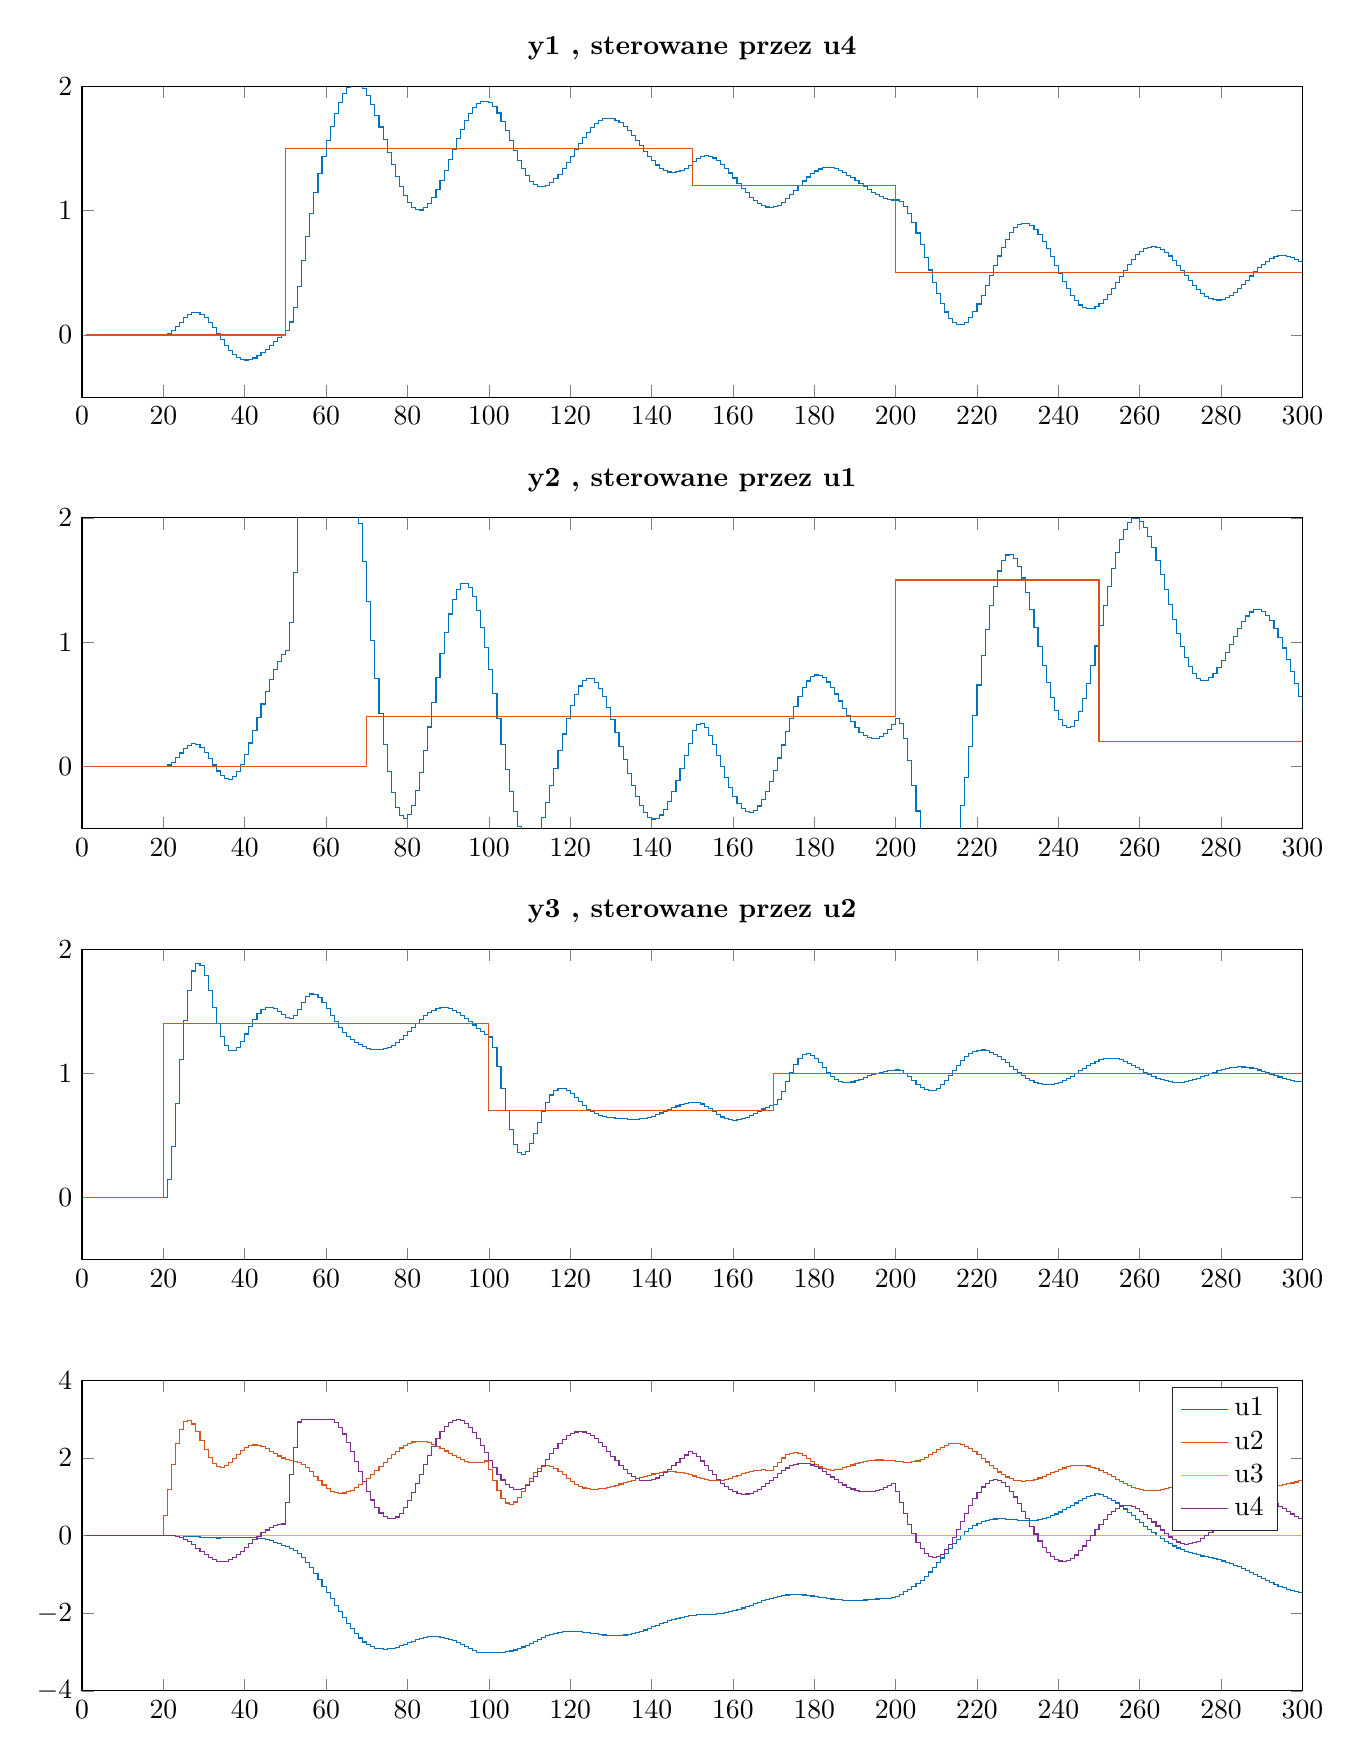
\begin{tikzpicture}

\begin{axis}[%
width=6.102in,
height=1.553in,
at={(1.024in,7.552in)},
scale only axis,
xmin=0,
xmax=300,
ymin=-0.5,
ymax=2,
axis background/.style={fill=white},
title style={font=\bfseries},
title={y1 , sterowane przez u4}
]
\addplot[const plot, color=mycolor1, forget plot] table[row sep=crcr] {%
1	0\\
2	0\\
3	0\\
4	0\\
5	0\\
6	0\\
7	0\\
8	0\\
9	0\\
10	0\\
11	0\\
12	0\\
13	0\\
14	0\\
15	0\\
16	0\\
17	0\\
18	0\\
19	0\\
20	0\\
21	0.0114581194369012\\
22	0.0352462992044872\\
23	0.0677484901461678\\
24	0.103603223453835\\
25	0.137160128214437\\
26	0.163320525296319\\
27	0.178189769449552\\
28	0.179461578592277\\
29	0.1665343266161\\
30	0.140394952392497\\
31	0.10332777921315\\
32	0.05851603714065\\
33	0.00960379673464971\\
34	-0.0397224986793789\\
35	-0.0860878818291958\\
36	-0.126689942324631\\
37	-0.159455880821655\\
38	-0.183099049917898\\
39	-0.197089721544304\\
40	-0.201561821702196\\
41	-0.197180151224861\\
42	-0.18499170908844\\
43	-0.166281055807683\\
44	-0.142444271013945\\
45	-0.114890039580126\\
46	-0.0849706711171832\\
47	-0.0539411121149932\\
48	-0.0229406672209462\\
49	0.00700964814939271\\
50	0.0350015379190751\\
51	0.103945672077657\\
52	0.223488165382759\\
53	0.390544643367417\\
54	0.597598669224736\\
55	0.795696798151239\\
56	0.978436657996233\\
57	1.14599517258156\\
58	1.298932060831\\
59	1.43812633865152\\
60	1.56466716438192\\
61	1.67974165891932\\
62	1.78350148501292\\
63	1.87243783353047\\
64	1.94363518409535\\
65	1.99482853491971\\
66	2.02449031803527\\
67	2.03189949001258\\
68	2.01717918010688\\
69	1.9812987536916\\
70	1.92603819266723\\
71	1.85415790126307\\
72	1.76887080997766\\
73	1.67381547498197\\
74	1.57294274092482\\
75	1.47035917040688\\
76	1.370154577211\\
77	1.27623444786242\\
78	1.19216472944924\\
79	1.12103556910895\\
80	1.06534926916178\\
81	1.02693623884774\\
82	1.00690120941556\\
83	1.00560052087565\\
84	1.02264994995175\\
85	1.05696137068256\\
86	1.10680554325447\\
87	1.16989751972057\\
88	1.24350053430421\\
89	1.32454380291838\\
90	1.4097493817435\\
91	1.49576311929149\\
92	1.57928477304154\\
93	1.65719254448684\\
94	1.72665760951832\\
95	1.78524467737332\\
96	1.83099519081466\\
97	1.86249046840293\\
98	1.87910687812647\\
99	1.88111221523565\\
100	1.86872508320594\\
101	1.8369578367796\\
102	1.78659688150793\\
103	1.72109769682731\\
104	1.64514584300549\\
105	1.56398310650012\\
106	1.48279865766227\\
107	1.40626291255131\\
108	1.33822864058447\\
109	1.28156838057952\\
110	1.23813509996244\\
111	1.20882135190178\\
112	1.19368631868924\\
113	1.19211948288943\\
114	1.20301314694936\\
115	1.22492227581084\\
116	1.25619773614101\\
117	1.29508664470662\\
118	1.33980018072876\\
119	1.38855417553891\\
120	1.43959074809114\\
121	1.49119022227494\\
122	1.54168182191949\\
123	1.58945964707589\\
124	1.63300772576839\\
125	1.67093503779109\\
126	1.70201877558704\\
127	1.72525207637889\\
128	1.73989122364525\\
129	1.74549692976511\\
130	1.74196471002532\\
131	1.7295403864407\\
132	1.70881820962967\\
133	1.6807207321716\\
134	1.64646119457286\\
135	1.60749061896791\\
136	1.5654329207039\\
137	1.52201207489952\\
138	1.47897569835909\\
139	1.43801935622977\\
140	1.40071553959119\\
141	1.36845066593582\\
142	1.34237271651446\\
143	1.3233513252657\\
144	1.3119513433163\\
145	1.30842017338993\\
146	1.3126885338343\\
147	1.32438378894662\\
148	1.34285457317293\\
149	1.36720513379904\\
150	1.39633760642119\\
151	1.42025760943156\\
152	1.43554246268621\\
153	1.44128911260867\\
154	1.43751056676193\\
155	1.42465865976923\\
156	1.40357594477419\\
157	1.37542545858048\\
158	1.34161251900599\\
159	1.30370474534055\\
160	1.26335463917748\\
161	1.22222784910409\\
162	1.18193904918657\\
163	1.14399636859965\\
164	1.10975459734406\\
165	1.08037697464143\\
166	1.0568052065128\\
167	1.03973738889811\\
168	1.02961364922188\\
169	1.02660948023638\\
170	1.03063685622229\\
171	1.04380855672111\\
172	1.06573131919532\\
173	1.09483725891323\\
174	1.12900347916468\\
175	1.16590251076554\\
176	1.2032259706048\\
177	1.23887153414433\\
178	1.27107431095471\\
179	1.29848062812329\\
180	1.32016981797081\\
181	1.33563431374686\\
182	1.34473079333566\\
183	1.34761538085379\\
184	1.34467445607611\\
185	1.33646000312692\\
186	1.32363525484144\\
187	1.30693320617404\\
188	1.28712781332609\\
189	1.26501565149484\\
190	1.24140460472009\\
191	1.21710579667062\\
192	1.19292532053313\\
193	1.1696531955382\\
194	1.14804814016004\\
195	1.12881798410391\\
196	1.1125966513818\\
197	1.09991949462687\\
198	1.09119926551026\\
199	1.08670514584225\\
200	1.0865470676354\\
201	1.07093461549265\\
202	1.03498917522666\\
203	0.979469185907536\\
204	0.907038193406519\\
205	0.82109009442238\\
206	0.725558524113182\\
207	0.624692925587123\\
208	0.522834459387087\\
209	0.424206320430704\\
210	0.332728337726977\\
211	0.251862521350685\\
212	0.184493072171187\\
213	0.132841681852541\\
214	0.0984169026115337\\
215	0.0819949990827965\\
216	0.0836289452577943\\
217	0.102681966435832\\
218	0.137882086152978\\
219	0.187394358071361\\
220	0.2489077047065\\
221	0.319733451178899\\
222	0.396912682545117\\
223	0.477329462734641\\
224	0.557826764110824\\
225	0.635321726994426\\
226	0.706916667763007\\
227	0.770002150790603\\
228	0.822348489910669\\
229	0.862182286049994\\
230	0.888245052460093\\
231	0.899831616988686\\
232	0.896806790355287\\
233	0.879599702422319\\
234	0.849176176868054\\
235	0.806990476715227\\
236	0.754918649487686\\
237	0.695176479371284\\
238	0.630225673616476\\
239	0.562672343520298\\
240	0.495162072249011\\
241	0.430275891049866\\
242	0.370431321970795\\
243	0.317792308195099\\
244	0.274191368433899\\
245	0.241066709824926\\
246	0.219416347003958\\
247	0.209770536381715\\
248	0.212183076084555\\
249	0.226241273352273\\
250	0.251093669521292\\
251	0.284705509158829\\
252	0.325285078017108\\
253	0.371000058364799\\
254	0.419913360421218\\
255	0.470021784107512\\
256	0.519333861866879\\
257	0.565944054767785\\
258	0.60810162796291\\
259	0.644272107696387\\
260	0.67318938482002\\
261	0.693896820846234\\
262	0.705776065803253\\
263	0.708562711808556\\
264	0.702348372057109\\
265	0.687569274895228\\
266	0.664981974793594\\
267	0.635627281254998\\
268	0.600783967148369\\
269	0.561914215319541\\
270	0.520603075759619\\
271	0.478494419305493\\
272	0.437225977984904\\
273	0.398366053259814\\
274	0.363354354360454\\
275	0.333449208080207\\
276	0.309683071996266\\
277	0.292827901894746\\
278	0.283371490443961\\
279	0.281505428364506\\
280	0.28712486215472\\
281	0.299839753751387\\
282	0.318996905719106\\
283	0.343711616929063\\
284	0.372907491919175\\
285	0.405362653092743\\
286	0.43976040647337\\
287	0.474742293675754\\
288	0.508961426799935\\
289	0.541134047863578\\
290	0.57008737608704\\
291	0.594801998173131\\
292	0.614447309691331\\
293	0.628408818821677\\
294	0.636306464499117\\
295	0.638003465768128\\
296	0.633605593631405\\
297	0.623451126480288\\
298	0.608092101388671\\
299	0.588267793153462\\
300	0.56487162943084\\
};
\addplot[const plot, color=mycolor2, forget plot] table[row sep=crcr] {%
1	0\\
2	0\\
3	0\\
4	0\\
5	0\\
6	0\\
7	0\\
8	0\\
9	0\\
10	0\\
11	0\\
12	0\\
13	0\\
14	0\\
15	0\\
16	0\\
17	0\\
18	0\\
19	0\\
20	0\\
21	0\\
22	0\\
23	0\\
24	0\\
25	0\\
26	0\\
27	0\\
28	0\\
29	0\\
30	0\\
31	0\\
32	0\\
33	0\\
34	0\\
35	0\\
36	0\\
37	0\\
38	0\\
39	0\\
40	0\\
41	0\\
42	0\\
43	0\\
44	0\\
45	0\\
46	0\\
47	0\\
48	0\\
49	0\\
50	1.5\\
51	1.5\\
52	1.5\\
53	1.5\\
54	1.5\\
55	1.5\\
56	1.5\\
57	1.5\\
58	1.5\\
59	1.5\\
60	1.5\\
61	1.5\\
62	1.5\\
63	1.5\\
64	1.5\\
65	1.5\\
66	1.5\\
67	1.5\\
68	1.5\\
69	1.5\\
70	1.5\\
71	1.5\\
72	1.5\\
73	1.5\\
74	1.5\\
75	1.5\\
76	1.5\\
77	1.5\\
78	1.5\\
79	1.5\\
80	1.5\\
81	1.5\\
82	1.5\\
83	1.5\\
84	1.5\\
85	1.5\\
86	1.5\\
87	1.5\\
88	1.5\\
89	1.5\\
90	1.5\\
91	1.5\\
92	1.5\\
93	1.5\\
94	1.5\\
95	1.5\\
96	1.5\\
97	1.5\\
98	1.5\\
99	1.5\\
100	1.5\\
101	1.5\\
102	1.5\\
103	1.5\\
104	1.5\\
105	1.5\\
106	1.5\\
107	1.5\\
108	1.5\\
109	1.5\\
110	1.5\\
111	1.5\\
112	1.5\\
113	1.5\\
114	1.5\\
115	1.5\\
116	1.5\\
117	1.5\\
118	1.5\\
119	1.5\\
120	1.5\\
121	1.5\\
122	1.5\\
123	1.5\\
124	1.5\\
125	1.5\\
126	1.5\\
127	1.5\\
128	1.5\\
129	1.5\\
130	1.5\\
131	1.5\\
132	1.5\\
133	1.5\\
134	1.5\\
135	1.5\\
136	1.5\\
137	1.5\\
138	1.5\\
139	1.5\\
140	1.5\\
141	1.5\\
142	1.5\\
143	1.5\\
144	1.5\\
145	1.5\\
146	1.5\\
147	1.5\\
148	1.5\\
149	1.5\\
150	1.2\\
151	1.2\\
152	1.2\\
153	1.2\\
154	1.2\\
155	1.2\\
156	1.2\\
157	1.2\\
158	1.2\\
159	1.2\\
160	1.2\\
161	1.2\\
162	1.2\\
163	1.2\\
164	1.2\\
165	1.2\\
166	1.2\\
167	1.2\\
168	1.2\\
169	1.2\\
170	1.2\\
171	1.2\\
172	1.2\\
173	1.2\\
174	1.2\\
175	1.2\\
176	1.2\\
177	1.2\\
178	1.2\\
179	1.2\\
180	1.2\\
181	1.2\\
182	1.2\\
183	1.2\\
184	1.2\\
185	1.2\\
186	1.2\\
187	1.2\\
188	1.2\\
189	1.2\\
190	1.2\\
191	1.2\\
192	1.2\\
193	1.2\\
194	1.2\\
195	1.2\\
196	1.2\\
197	1.2\\
198	1.2\\
199	1.2\\
200	0.5\\
201	0.5\\
202	0.5\\
203	0.5\\
204	0.5\\
205	0.5\\
206	0.5\\
207	0.5\\
208	0.5\\
209	0.5\\
210	0.5\\
211	0.5\\
212	0.5\\
213	0.5\\
214	0.5\\
215	0.5\\
216	0.5\\
217	0.5\\
218	0.5\\
219	0.5\\
220	0.5\\
221	0.5\\
222	0.5\\
223	0.5\\
224	0.5\\
225	0.5\\
226	0.5\\
227	0.5\\
228	0.5\\
229	0.5\\
230	0.5\\
231	0.5\\
232	0.5\\
233	0.5\\
234	0.5\\
235	0.5\\
236	0.5\\
237	0.5\\
238	0.5\\
239	0.5\\
240	0.5\\
241	0.5\\
242	0.5\\
243	0.5\\
244	0.5\\
245	0.5\\
246	0.5\\
247	0.5\\
248	0.5\\
249	0.5\\
250	0.5\\
251	0.5\\
252	0.5\\
253	0.5\\
254	0.5\\
255	0.5\\
256	0.5\\
257	0.5\\
258	0.5\\
259	0.5\\
260	0.5\\
261	0.5\\
262	0.5\\
263	0.5\\
264	0.5\\
265	0.5\\
266	0.5\\
267	0.5\\
268	0.5\\
269	0.5\\
270	0.5\\
271	0.5\\
272	0.5\\
273	0.5\\
274	0.5\\
275	0.5\\
276	0.5\\
277	0.5\\
278	0.5\\
279	0.5\\
280	0.5\\
281	0.5\\
282	0.5\\
283	0.5\\
284	0.5\\
285	0.5\\
286	0.5\\
287	0.5\\
288	0.5\\
289	0.5\\
290	0.5\\
291	0.5\\
292	0.5\\
293	0.5\\
294	0.5\\
295	0.5\\
296	0.5\\
297	0.5\\
298	0.5\\
299	0.5\\
300	0.5\\
};
\end{axis}

\begin{axis}[%
width=6.102in,
height=1.553in,
at={(1.024in,5.395in)},
scale only axis,
xmin=0,
xmax=300,
ymin=-0.5,
ymax=2,
axis background/.style={fill=white},
title style={font=\bfseries},
title={y2 , sterowane przez u1}
]
\addplot[const plot, color=mycolor1, forget plot] table[row sep=crcr] {%
1	0\\
2	0\\
3	0\\
4	0\\
5	0\\
6	0\\
7	0\\
8	0\\
9	0\\
10	0\\
11	0\\
12	0\\
13	0\\
14	0\\
15	0\\
16	0\\
17	0\\
18	0\\
19	0\\
20	0\\
21	0.0105699306087332\\
22	0.0344208390223349\\
23	0.0689011197977337\\
24	0.107955166598362\\
25	0.144170861661471\\
26	0.170521212117058\\
27	0.181731894788386\\
28	0.175115670399834\\
29	0.150863862971588\\
30	0.111859475172388\\
31	0.0631245303254672\\
32	0.0110394104118058\\
33	-0.0375251109048523\\
34	-0.0760377673269987\\
35	-0.0990012980728244\\
36	-0.1024489155195\\
37	-0.0842157947736674\\
38	-0.0439906335293748\\
39	0.0168226146332741\\
40	0.0953863326265939\\
41	0.187800187751842\\
42	0.289508011554615\\
43	0.39569401324904\\
44	0.501632661578429\\
45	0.602969374606704\\
46	0.695921830106785\\
47	0.777402690363395\\
48	0.845072814548994\\
49	0.897339165461868\\
50	0.933313666184573\\
51	1.16020538749771\\
52	1.5583808468053\\
53	2.05950372562056\\
54	2.60150829688574\\
55	2.94869431107951\\
56	3.14599670890162\\
57	3.24861779685659\\
58	3.29022044662744\\
59	3.29155592953236\\
60	3.26561962849917\\
61	3.22073534012211\\
62	3.15749228626483\\
63	3.05938753585428\\
64	2.91890160572987\\
65	2.73442906629392\\
66	2.50850163562071\\
67	2.24662282808777\\
68	1.95642488297528\\
69	1.64700611203031\\
70	1.32836684820227\\
71	1.0116225224599\\
72	0.70726719992172\\
73	0.425056386664036\\
74	0.173744645673658\\
75	-0.039214456331446\\
76	-0.207945712921669\\
77	-0.328361446850166\\
78	-0.398294620802523\\
79	-0.417550702247379\\
80	-0.38787713085102\\
81	-0.312853319805292\\
82	-0.197707849207666\\
83	-0.0490726816653588\\
84	0.125313287864178\\
85	0.316937314287024\\
86	0.516867532993072\\
87	0.716114141568382\\
88	0.905982288168858\\
89	1.07840295023141\\
90	1.22622958858692\\
91	1.34349023266803\\
92	1.42558679198633\\
93	1.46943570380107\\
94	1.47354643117808\\
95	1.43803674116744\\
96	1.36458604772014\\
97	1.2563303315604\\
98	1.11834092893243\\
99	0.957643755687471\\
100	0.780173524460053\\
101	0.587023774046827\\
102	0.383430172945113\\
103	0.177295632042849\\
104	-0.0220127441242369\\
105	-0.204507191232089\\
106	-0.360956334827732\\
107	-0.483889413921107\\
108	-0.568191584331081\\
109	-0.611381349385619\\
110	-0.613596918435549\\
111	-0.57734659891566\\
112	-0.507092831992189\\
113	-0.408742688754356\\
114	-0.289111761618096\\
115	-0.155416025979801\\
116	-0.0148303217742552\\
117	0.125864625803876\\
118	0.260539983229616\\
119	0.383886901224403\\
120	0.49150869286823\\
121	0.579955037378289\\
122	0.646716661104408\\
123	0.690196621852651\\
124	0.709670189195767\\
125	0.705240427535726\\
126	0.677791885598921\\
127	0.628940989182512\\
128	0.560979262967887\\
129	0.476804532375357\\
130	0.379835690999301\\
131	0.273908187743654\\
132	0.163149698166771\\
133	0.0518380610405595\\
134	-0.0557539303699277\\
135	-0.155520234655424\\
136	-0.24368174972206\\
137	-0.316936407910323\\
138	-0.372590870713881\\
139	-0.408666517946903\\
140	-0.423974012078491\\
141	-0.418152692049958\\
142	-0.391673204698695\\
143	-0.34580392054144\\
144	-0.282543639126258\\
145	-0.20452474403733\\
146	-0.114892241349494\\
147	-0.0171649744006532\\
148	0.0849142433923883\\
149	0.187532763883159\\
150	0.286959946161178\\
151	0.33819931616075\\
152	0.342091384895358\\
153	0.309782285295243\\
154	0.251804934498354\\
155	0.176461544018121\\
156	0.0907735012878417\\
157	0.000920237180046218\\
158	-0.0875889454523508\\
159	-0.169885855022509\\
160	-0.241782735205747\\
161	-0.299834031648909\\
162	-0.341393430272608\\
163	-0.364651296751035\\
164	-0.368645674999069\\
165	-0.35324511388585\\
166	-0.319104683815451\\
167	-0.267598251720975\\
168	-0.200730874352895\\
169	-0.121035401331662\\
170	-0.0314573159099687\\
171	0.0670333173855378\\
172	0.171620111838999\\
173	0.278303207595625\\
174	0.382444057315703\\
175	0.479322882187218\\
176	0.56462076357312\\
177	0.634808403873443\\
178	0.68740436910824\\
179	0.721097995500388\\
180	0.735748637487933\\
181	0.732283939250454\\
182	0.71252604914081\\
183	0.678976247687632\\
184	0.634586125096449\\
185	0.582538351603463\\
186	0.526053473047478\\
187	0.468232203131184\\
188	0.411936334201706\\
189	0.359706322527943\\
190	0.313710178931727\\
191	0.275716572266832\\
192	0.247084850962492\\
193	0.228765658957834\\
194	0.221307533378875\\
195	0.224866878943671\\
196	0.239220627003285\\
197	0.263782408515123\\
198	0.297624019333228\\
199	0.33950427026122\\
200	0.387907034720279\\
201	0.346261385442663\\
202	0.222460531663037\\
203	0.046648356207377\\
204	-0.154011957173843\\
205	-0.359042419395874\\
206	-0.552406238597395\\
207	-0.721405114586762\\
208	-0.856154421516372\\
209	-0.949351916306527\\
210	-0.996173288132129\\
211	-0.994195649826503\\
212	-0.943294285159941\\
213	-0.845486773331783\\
214	-0.704717157530366\\
215	-0.526584343578931\\
216	-0.318025541173194\\
217	-0.0869687880676455\\
218	0.158030472544754\\
219	0.408154327102019\\
220	0.654675781524992\\
221	0.8892893156202\\
222	1.10440917197595\\
223	1.2934277332354\\
224	1.45092798294303\\
225	1.57284555057529\\
226	1.65657726065696\\
227	1.70103450405071\\
228	1.70664118394728\\
229	1.67527749325997\\
230	1.61017235486825\\
231	1.51574896804388\\
232	1.39742949025912\\
233	1.26140635940546\\
234	1.11438903379895\\
235	0.963335905335035\\
236	0.815181747424203\\
237	0.676571238699163\\
238	0.553608828536613\\
239	0.451634483874654\\
240	0.375033710595886\\
241	0.327088734648944\\
242	0.309875936256123\\
243	0.324212647004718\\
244	0.369654343267963\\
245	0.444541199460382\\
246	0.546090994773343\\
247	0.670533580693344\\
248	0.813280583560282\\
249	0.969122790678379\\
250	1.1324467873118\\
251	1.29511603114166\\
252	1.45080771774106\\
253	1.5941862085682\\
254	1.72065676157424\\
255	1.82637524280697\\
256	1.90834863107285\\
257	1.96450803848148\\
258	1.99375195441402\\
259	1.99595661136619\\
260	1.97195240278949\\
261	1.92346718904819\\
262	1.85303883551717\\
263	1.7639005526776\\
264	1.65984360467208\\
265	1.5450627398289\\
266	1.4239902743479\\
267	1.30112511902081\\
268	1.18086316657697\\
269	1.06733534545953\\
270	0.964259293576865\\
271	0.874810022025024\\
272	0.80151414438784\\
273	0.746171273439401\\
274	0.709805074941886\\
275	0.692645266103373\\
276	0.694140606955181\\
277	0.713001710618139\\
278	0.747271345661203\\
279	0.794418868567087\\
280	0.851454547988054\\
281	0.915058857759354\\
282	0.981721345639153\\
283	1.04788344237552\\
284	1.11007956370972\\
285	1.16507106938749\\
286	1.20996806245058\\
287	1.24233461567422\\
288	1.26027377038924\\
289	1.26248953167485\\
290	1.24832404536565\\
291	1.21776914709055\\
292	1.17145248202417\\
293	1.11059936773341\\
294	1.0369724754911\\
295	0.952792205435081\\
296	0.860641300420193\\
297	0.763357760361792\\
298	0.663920467547664\\
299	0.565332104711786\\
300	0.470503939388236\\
};
\addplot[const plot, color=mycolor2, forget plot] table[row sep=crcr] {%
1	0\\
2	0\\
3	0\\
4	0\\
5	0\\
6	0\\
7	0\\
8	0\\
9	0\\
10	0\\
11	0\\
12	0\\
13	0\\
14	0\\
15	0\\
16	0\\
17	0\\
18	0\\
19	0\\
20	0\\
21	0\\
22	0\\
23	0\\
24	0\\
25	0\\
26	0\\
27	0\\
28	0\\
29	0\\
30	0\\
31	0\\
32	0\\
33	0\\
34	0\\
35	0\\
36	0\\
37	0\\
38	0\\
39	0\\
40	0\\
41	0\\
42	0\\
43	0\\
44	0\\
45	0\\
46	0\\
47	0\\
48	0\\
49	0\\
50	0\\
51	0\\
52	0\\
53	0\\
54	0\\
55	0\\
56	0\\
57	0\\
58	0\\
59	0\\
60	0\\
61	0\\
62	0\\
63	0\\
64	0\\
65	0\\
66	0\\
67	0\\
68	0\\
69	0\\
70	0.4\\
71	0.4\\
72	0.4\\
73	0.4\\
74	0.4\\
75	0.4\\
76	0.4\\
77	0.4\\
78	0.4\\
79	0.4\\
80	0.4\\
81	0.4\\
82	0.4\\
83	0.4\\
84	0.4\\
85	0.4\\
86	0.4\\
87	0.4\\
88	0.4\\
89	0.4\\
90	0.4\\
91	0.4\\
92	0.4\\
93	0.4\\
94	0.4\\
95	0.4\\
96	0.4\\
97	0.4\\
98	0.4\\
99	0.4\\
100	0.4\\
101	0.4\\
102	0.4\\
103	0.4\\
104	0.4\\
105	0.4\\
106	0.4\\
107	0.4\\
108	0.4\\
109	0.4\\
110	0.4\\
111	0.4\\
112	0.4\\
113	0.4\\
114	0.4\\
115	0.4\\
116	0.4\\
117	0.4\\
118	0.4\\
119	0.4\\
120	0.4\\
121	0.4\\
122	0.4\\
123	0.4\\
124	0.4\\
125	0.4\\
126	0.4\\
127	0.4\\
128	0.4\\
129	0.4\\
130	0.4\\
131	0.4\\
132	0.4\\
133	0.4\\
134	0.4\\
135	0.4\\
136	0.4\\
137	0.4\\
138	0.4\\
139	0.4\\
140	0.4\\
141	0.4\\
142	0.4\\
143	0.4\\
144	0.4\\
145	0.4\\
146	0.4\\
147	0.4\\
148	0.4\\
149	0.4\\
150	0.4\\
151	0.4\\
152	0.4\\
153	0.4\\
154	0.4\\
155	0.4\\
156	0.4\\
157	0.4\\
158	0.4\\
159	0.4\\
160	0.4\\
161	0.4\\
162	0.4\\
163	0.4\\
164	0.4\\
165	0.4\\
166	0.4\\
167	0.4\\
168	0.4\\
169	0.4\\
170	0.4\\
171	0.4\\
172	0.4\\
173	0.4\\
174	0.4\\
175	0.4\\
176	0.4\\
177	0.4\\
178	0.4\\
179	0.4\\
180	0.4\\
181	0.4\\
182	0.4\\
183	0.4\\
184	0.4\\
185	0.4\\
186	0.4\\
187	0.4\\
188	0.4\\
189	0.4\\
190	0.4\\
191	0.4\\
192	0.4\\
193	0.4\\
194	0.4\\
195	0.4\\
196	0.4\\
197	0.4\\
198	0.4\\
199	0.4\\
200	1.5\\
201	1.5\\
202	1.5\\
203	1.5\\
204	1.5\\
205	1.5\\
206	1.5\\
207	1.5\\
208	1.5\\
209	1.5\\
210	1.5\\
211	1.5\\
212	1.5\\
213	1.5\\
214	1.5\\
215	1.5\\
216	1.5\\
217	1.5\\
218	1.5\\
219	1.5\\
220	1.5\\
221	1.5\\
222	1.5\\
223	1.5\\
224	1.5\\
225	1.5\\
226	1.5\\
227	1.5\\
228	1.5\\
229	1.5\\
230	1.5\\
231	1.5\\
232	1.5\\
233	1.5\\
234	1.5\\
235	1.5\\
236	1.5\\
237	1.5\\
238	1.5\\
239	1.5\\
240	1.5\\
241	1.5\\
242	1.5\\
243	1.5\\
244	1.5\\
245	1.5\\
246	1.5\\
247	1.5\\
248	1.5\\
249	1.5\\
250	0.2\\
251	0.2\\
252	0.2\\
253	0.2\\
254	0.2\\
255	0.2\\
256	0.2\\
257	0.2\\
258	0.2\\
259	0.2\\
260	0.2\\
261	0.2\\
262	0.2\\
263	0.2\\
264	0.2\\
265	0.2\\
266	0.2\\
267	0.2\\
268	0.2\\
269	0.2\\
270	0.2\\
271	0.2\\
272	0.2\\
273	0.2\\
274	0.2\\
275	0.2\\
276	0.2\\
277	0.2\\
278	0.2\\
279	0.2\\
280	0.2\\
281	0.2\\
282	0.2\\
283	0.2\\
284	0.2\\
285	0.2\\
286	0.2\\
287	0.2\\
288	0.2\\
289	0.2\\
290	0.2\\
291	0.2\\
292	0.2\\
293	0.2\\
294	0.2\\
295	0.2\\
296	0.2\\
297	0.2\\
298	0.2\\
299	0.2\\
300	0.2\\
};
\end{axis}

\begin{axis}[%
width=6.102in,
height=1.553in,
at={(1.024in,3.239in)},
scale only axis,
xmin=0,
xmax=300,
ymin=-0.5,
ymax=2,
axis background/.style={fill=white},
title style={font=\bfseries},
title={y3 , sterowane przez u2}
]
\addplot[const plot, color=mycolor1, forget plot] table[row sep=crcr] {%
1	0\\
2	0\\
3	0\\
4	0\\
5	0\\
6	0\\
7	0\\
8	0\\
9	0\\
10	0\\
11	0\\
12	0\\
13	0\\
14	0\\
15	0\\
16	0\\
17	0\\
18	0\\
19	0\\
20	0\\
21	0.142671982788199\\
22	0.414294892302412\\
23	0.757136535090792\\
24	1.11073510318054\\
25	1.42618799032908\\
26	1.66965012779232\\
27	1.8236462974704\\
28	1.88601949665447\\
29	1.86710715037528\\
30	1.78587320488042\\
31	1.665706181078\\
32	1.53049223072861\\
33	1.40141340045136\\
34	1.29473680768947\\
35	1.22067922829355\\
36	1.18327630416922\\
37	1.18107089333081\\
38	1.20836749124967\\
39	1.25677826832363\\
40	1.31680445143583\\
41	1.37924415138103\\
42	1.436282284589\\
43	1.48218817646995\\
44	1.51361168753105\\
45	1.5295218470913\\
46	1.53086865510872\\
47	1.52006756593917\\
48	1.50040841085981\\
49	1.47547924936994\\
50	1.44867506845136\\
51	1.44413658009783\\
52	1.46699779499627\\
53	1.51303788066527\\
54	1.57327861326534\\
55	1.61741853632854\\
56	1.63819155295768\\
57	1.63483006538685\\
58	1.61010509853541\\
59	1.56934146151875\\
60	1.51913934879081\\
61	1.46620358847911\\
62	1.41591104206819\\
63	1.37049669866696\\
64	1.33106012019421\\
65	1.2977503607478\\
66	1.27009975229439\\
67	1.24736226478573\\
68	1.22879688681636\\
69	1.21386784511786\\
70	1.20234984339944\\
71	1.19448407910227\\
72	1.1906716353801\\
73	1.1914105749499\\
74	1.19718172380476\\
75	1.20832541024739\\
76	1.22493518123945\\
77	1.24678704765233\\
78	1.27331056883884\\
79	1.30360210158807\\
80	1.33647525066415\\
81	1.37053975138506\\
82	1.40429791199375\\
83	1.43624727891617\\
84	1.46497910851254\\
85	1.48926416105458\\
86	1.5081198534911\\
87	1.52085550794809\\
88	1.52709496584573\\
89	1.52677794866604\\
90	1.52014308650815\\
91	1.50769645687824\\
92	1.49016981669136\\
93	1.46847257055766\\
94	1.44364103430181\\
95	1.41678787093596\\
96	1.38905383261967\\
97	1.36156324581596\\
98	1.33550928748627\\
99	1.31216559008835\\
100	1.2922987914005\\
101	1.20513134816405\\
102	1.05787553863966\\
103	0.879561727532468\\
104	0.700421867303169\\
105	0.544846396081888\\
106	0.429596796086128\\
107	0.363131637530745\\
108	0.346131197135364\\
109	0.37291084216255\\
110	0.433362474177556\\
111	0.51507029126703\\
112	0.605296489757553\\
113	0.69261095190886\\
114	0.768030389344058\\
115	0.825622445137743\\
116	0.862607626708829\\
117	0.879049294744136\\
118	0.877255987982982\\
119	0.861031501184614\\
120	0.834899604300729\\
121	0.803407212031581\\
122	0.770578130404933\\
123	0.739555061539137\\
124	0.712435344746738\\
125	0.690279647417808\\
126	0.673254669611744\\
127	0.660861578716216\\
128	0.652200756098246\\
129	0.64622898721071\\
130	0.641975378704495\\
131	0.638694787393846\\
132	0.635950296419264\\
133	0.633627566461165\\
134	0.631892550375539\\
135	0.631109490635295\\
136	0.63173825982014\\
137	0.634229330703048\\
138	0.638931649769091\\
139	0.646024264506617\\
140	0.65547756442511\\
141	0.667045186725664\\
142	0.680283585974526\\
143	0.694593338001469\\
144	0.709274591433298\\
145	0.723588654850321\\
146	0.736818325584173\\
147	0.748320946396093\\
148	0.757569998771706\\
149	0.764182996233529\\
150	0.767935264899813\\
151	0.764500567099536\\
152	0.753348732683906\\
153	0.735783103830551\\
154	0.714008063306285\\
155	0.690578646872215\\
156	0.668036613804811\\
157	0.648600568681256\\
158	0.633949551847444\\
159	0.625109445754317\\
160	0.622436116225082\\
161	0.625678544971056\\
162	0.634098703598476\\
163	0.646622669767856\\
164	0.661998907136662\\
165	0.678943784472865\\
166	0.696260201381003\\
167	0.712921538918878\\
168	0.728119134240467\\
169	0.741276399915519\\
170	0.752036160506282\\
171	0.790802193605909\\
172	0.854613239825157\\
173	0.931182483465484\\
174	1.00770564625364\\
175	1.07389329456736\\
176	1.12270098668307\\
177	1.15060081398179\\
178	1.15735444219689\\
179	1.14541177045645\\
180	1.1190881808783\\
181	1.08366968518091\\
182	1.04457420003417\\
183	1.00666396369756\\
184	0.973765474093489\\
185	0.948415350993203\\
186	0.931817943749653\\
187	0.923976403636227\\
188	0.923944681230217\\
189	0.930143315624749\\
190	0.94068556832017\\
191	0.953670252535411\\
192	0.967411006085719\\
193	0.980586289591424\\
194	0.992307954390852\\
195	1.00211726379573\\
196	1.00992485677925\\
197	1.01591503290579\\
198	1.02043516642555\\
199	1.02388867611566\\
200	1.02664566679652\\
201	1.01943001110073\\
202	1.00106267609948\\
203	0.974057865520315\\
204	0.942586747966382\\
205	0.911329670966572\\
206	0.884760520020385\\
207	0.866552777561793\\
208	0.859186268458603\\
209	0.863768916204781\\
210	0.880056302493407\\
211	0.906630709099233\\
212	0.941188961308867\\
213	0.980884861797314\\
214	1.02267596328547\\
215	1.06363385091191\\
216	1.1011896833542\\
217	1.13330023749674\\
218	1.158532219488\\
219	1.17607276539094\\
220	1.18568106410357\\
221	1.18759966869805\\
222	1.18244457481169\\
223	1.17109113958611\\
224	1.15456919388945\\
225	1.13397612012037\\
226	1.11041201563581\\
227	1.08493696925322\\
228	1.05854737047972\\
229	1.03216625383026\\
230	1.00664195819044\\
231	0.982749697224137\\
232	0.961191727289951\\
233	0.942593349025391\\
234	0.927493673072589\\
235	0.91633164661259\\
236	0.909429072202635\\
237	0.906973133264965\\
238	0.909001233352826\\
239	0.915390792680284\\
240	0.925856112923024\\
241	0.939953640209171\\
242	0.957096058132852\\
243	0.976574751945319\\
244	0.997589404942658\\
245	1.01928289166011\\
246	1.04077925976714\\
247	1.0612224517434\\
248	1.07981349000979\\
249	1.09584409727628\\
250	1.10872509826497\\
251	1.11754719340838\\
252	1.12189370582293\\
253	1.12168586419597\\
254	1.11710562351055\\
255	1.10854160396882\\
256	1.09654292328449\\
257	1.08176981201597\\
258	1.06494681066737\\
259	1.04682165695467\\
260	1.0281314169382\\
261	1.00957616055438\\
262	0.991799534929519\\
263	0.97537501254278\\
264	0.960796375254525\\
265	0.948471081455659\\
266	0.938715464650575\\
267	0.931751128475497\\
268	0.927702340405931\\
269	0.926594605375062\\
270	0.928354866146166\\
271	0.932813901214532\\
272	0.939711470488895\\
273	0.948704612542433\\
274	0.959379258400925\\
275	0.971265037248963\\
276	0.983852851958996\\
277	0.996614535463177\\
278	1.0090236926983\\
279	1.02057670639795\\
280	1.03081284630074\\
281	1.03933246789537\\
282	1.04581240770346\\
283	1.05001786053966\\
284	1.05181024034664\\
285	1.05115075975146\\
286	1.04809969573811\\
287	1.04281152422169\\
288	1.03552629326799\\
289	1.02655775585393\\
290	1.01627889495739\\
291	1.00510554623073\\
292	0.993478858842593\\
293	0.981847337148375\\
294	0.970649179351967\\
295	0.960295579103126\\
296	0.951155586631253\\
297	0.943543041660698\\
298	0.937705994570155\\
299	0.933818928188618\\
300	0.931977983116255\\
};
\addplot[const plot, color=mycolor2, forget plot] table[row sep=crcr] {%
1	0\\
2	0\\
3	0\\
4	0\\
5	0\\
6	0\\
7	0\\
8	0\\
9	0\\
10	0\\
11	0\\
12	0\\
13	0\\
14	0\\
15	0\\
16	0\\
17	0\\
18	0\\
19	0\\
20	1.4\\
21	1.4\\
22	1.4\\
23	1.4\\
24	1.4\\
25	1.4\\
26	1.4\\
27	1.4\\
28	1.4\\
29	1.4\\
30	1.4\\
31	1.4\\
32	1.4\\
33	1.4\\
34	1.4\\
35	1.4\\
36	1.4\\
37	1.4\\
38	1.4\\
39	1.4\\
40	1.4\\
41	1.4\\
42	1.4\\
43	1.4\\
44	1.4\\
45	1.4\\
46	1.4\\
47	1.4\\
48	1.4\\
49	1.4\\
50	1.4\\
51	1.4\\
52	1.4\\
53	1.4\\
54	1.4\\
55	1.4\\
56	1.4\\
57	1.4\\
58	1.4\\
59	1.4\\
60	1.4\\
61	1.4\\
62	1.4\\
63	1.4\\
64	1.4\\
65	1.4\\
66	1.4\\
67	1.4\\
68	1.4\\
69	1.4\\
70	1.4\\
71	1.4\\
72	1.4\\
73	1.4\\
74	1.4\\
75	1.4\\
76	1.4\\
77	1.4\\
78	1.4\\
79	1.4\\
80	1.4\\
81	1.4\\
82	1.4\\
83	1.4\\
84	1.4\\
85	1.4\\
86	1.4\\
87	1.4\\
88	1.4\\
89	1.4\\
90	1.4\\
91	1.4\\
92	1.4\\
93	1.4\\
94	1.4\\
95	1.4\\
96	1.4\\
97	1.4\\
98	1.4\\
99	1.4\\
100	0.7\\
101	0.7\\
102	0.7\\
103	0.7\\
104	0.7\\
105	0.7\\
106	0.7\\
107	0.7\\
108	0.7\\
109	0.7\\
110	0.7\\
111	0.7\\
112	0.7\\
113	0.7\\
114	0.7\\
115	0.7\\
116	0.7\\
117	0.7\\
118	0.7\\
119	0.7\\
120	0.7\\
121	0.7\\
122	0.7\\
123	0.7\\
124	0.7\\
125	0.7\\
126	0.7\\
127	0.7\\
128	0.7\\
129	0.7\\
130	0.7\\
131	0.7\\
132	0.7\\
133	0.7\\
134	0.7\\
135	0.7\\
136	0.7\\
137	0.7\\
138	0.7\\
139	0.7\\
140	0.7\\
141	0.7\\
142	0.7\\
143	0.7\\
144	0.7\\
145	0.7\\
146	0.7\\
147	0.7\\
148	0.7\\
149	0.7\\
150	0.7\\
151	0.7\\
152	0.7\\
153	0.7\\
154	0.7\\
155	0.7\\
156	0.7\\
157	0.7\\
158	0.7\\
159	0.7\\
160	0.7\\
161	0.7\\
162	0.7\\
163	0.7\\
164	0.7\\
165	0.7\\
166	0.7\\
167	0.7\\
168	0.7\\
169	0.7\\
170	1\\
171	1\\
172	1\\
173	1\\
174	1\\
175	1\\
176	1\\
177	1\\
178	1\\
179	1\\
180	1\\
181	1\\
182	1\\
183	1\\
184	1\\
185	1\\
186	1\\
187	1\\
188	1\\
189	1\\
190	1\\
191	1\\
192	1\\
193	1\\
194	1\\
195	1\\
196	1\\
197	1\\
198	1\\
199	1\\
200	1\\
201	1\\
202	1\\
203	1\\
204	1\\
205	1\\
206	1\\
207	1\\
208	1\\
209	1\\
210	1\\
211	1\\
212	1\\
213	1\\
214	1\\
215	1\\
216	1\\
217	1\\
218	1\\
219	1\\
220	1\\
221	1\\
222	1\\
223	1\\
224	1\\
225	1\\
226	1\\
227	1\\
228	1\\
229	1\\
230	1\\
231	1\\
232	1\\
233	1\\
234	1\\
235	1\\
236	1\\
237	1\\
238	1\\
239	1\\
240	1\\
241	1\\
242	1\\
243	1\\
244	1\\
245	1\\
246	1\\
247	1\\
248	1\\
249	1\\
250	1\\
251	1\\
252	1\\
253	1\\
254	1\\
255	1\\
256	1\\
257	1\\
258	1\\
259	1\\
260	1\\
261	1\\
262	1\\
263	1\\
264	1\\
265	1\\
266	1\\
267	1\\
268	1\\
269	1\\
270	1\\
271	1\\
272	1\\
273	1\\
274	1\\
275	1\\
276	1\\
277	1\\
278	1\\
279	1\\
280	1\\
281	1\\
282	1\\
283	1\\
284	1\\
285	1\\
286	1\\
287	1\\
288	1\\
289	1\\
290	1\\
291	1\\
292	1\\
293	1\\
294	1\\
295	1\\
296	1\\
297	1\\
298	1\\
299	1\\
300	1\\
};
\end{axis}

\begin{axis}[%
width=6.102in,
height=1.553in,
at={(1.024in,1.083in)},
scale only axis,
xmin=0,
xmax=300,
ymin=-4,
ymax=4,
axis background/.style={fill=white},
legend style={legend cell align=left, align=left, draw=white!15!black}
]
\addplot[const plot, color=mycolor1] table[row sep=crcr] {%
1	0\\
2	0\\
3	0\\
4	0\\
5	0\\
6	0\\
7	0\\
8	0\\
9	0\\
10	0\\
11	0\\
12	0\\
13	0\\
14	0\\
15	0\\
16	0\\
17	0\\
18	0\\
19	0\\
20	0\\
21	0\\
22	-0.000391087432523129\\
23	-0.00178092771304559\\
24	-0.00473003823602488\\
25	-0.00955113339598402\\
26	-0.0162107643496359\\
27	-0.0243218390094399\\
28	-0.0332099941732208\\
29	-0.042029367244921\\
30	-0.0499010663388447\\
31	-0.0560496007537102\\
32	-0.059917390328592\\
33	-0.0612439372977537\\
34	-0.060103190769455\\
35	-0.0568990959792263\\
36	-0.0523245822881251\\
37	-0.0472928826004485\\
38	-0.0428519575269627\\
39	-0.0400930325128264\\
40	-0.0400631406958871\\
41	-0.0436895024969784\\
42	-0.0517210043319556\\
43	-0.0646893754899998\\
44	-0.0828902424828187\\
45	-0.106382301130069\\
46	-0.135001515294378\\
47	-0.16838655145216\\
48	-0.206011529875993\\
49	-0.247222497268517\\
50	-0.291274652731372\\
51	-0.33736813482938\\
52	-0.392356862825749\\
53	-0.464645840752389\\
54	-0.560310078690204\\
55	-0.682337188350413\\
56	-0.824174476577339\\
57	-0.978215008822345\\
58	-1.13891721972612\\
59	-1.30268216543456\\
60	-1.46715939533387\\
61	-1.63077487770645\\
62	-1.79244701306352\\
63	-1.95123355565366\\
64	-2.10560478030943\\
65	-2.25357238718836\\
66	-2.39297295537597\\
67	-2.52170403883463\\
68	-2.63789145959829\\
69	-2.74000903464859\\
70	-2.81216218016261\\
71	-2.86414167054438\\
72	-2.89947775142968\\
73	-2.91943121927025\\
74	-2.92496148982088\\
75	-2.91748019636395\\
76	-2.89879056535542\\
77	-2.87101270424902\\
78	-2.83649749896077\\
79	-2.79773273064988\\
80	-2.7572453909442\\
81	-2.71750429013638\\
82	-2.68082696745973\\
83	-2.64929463625949\\
84	-2.62467845405697\\
85	-2.60837983051121\\
86	-2.60138681194301\\
87	-2.60424784769664\\
88	-2.61706348842617\\
89	-2.63949582371165\\
90	-2.67079476632321\\
91	-2.70983965812981\\
92	-2.75519412811344\\
93	-2.80517169115346\\
94	-2.85790924737129\\
95	-2.91144543165066\\
96	-2.96380067322442\\
97	-3\\
98	-3\\
99	-3\\
100	-3\\
101	-3\\
102	-3\\
103	-3\\
104	-2.99195171783608\\
105	-2.97385435860184\\
106	-2.94640004360497\\
107	-2.91075105462454\\
108	-2.86846761224389\\
109	-2.82139982740086\\
110	-2.7715608312181\\
111	-2.72099616722409\\
112	-2.67166201426264\\
113	-2.62532157305399\\
114	-2.58346537922033\\
115	-2.54725788880018\\
116	-2.51750978108362\\
117	-2.49467325936896\\
118	-2.47885628493223\\
119	-2.46985111455202\\
120	-2.46717259896445\\
121	-2.4701022564805\\
122	-2.4777349622875\\
123	-2.48902600154526\\
124	-2.50283706990071\\
125	-2.51798046306355\\
126	-2.53326112420723\\
127	-2.54751640905567\\
128	-2.55965341725208\\
129	-2.5686835846341\\
130	-2.573754006203\\
131	-2.57417473515204\\
132	-2.5694411397643\\
133	-2.55925034004365\\
134	-2.54351081135747\\
135	-2.52234443400156\\
136	-2.49608056820732\\
137	-2.46524211302566\\
138	-2.43052392621672\\
139	-2.39276440001385\\
140	-2.35291136645614\\
141	-2.31198381457039\\
142	-2.27103111779579\\
143	-2.23109158158523\\
144	-2.19315212588941\\
145	-2.15811082170639\\
146	-2.12674381830553\\
147	-2.09967794591294\\
148	-2.0773699777172\\
149	-2.06009320552161\\
150	-2.0479316445138\\
151	-2.04078185141126\\
152	-2.03682685104475\\
153	-2.03377834465597\\
154	-2.02967969307806\\
155	-2.02308826356254\\
156	-2.01300675954128\\
157	-1.99881006594213\\
158	-1.98019554631999\\
159	-1.95714642494981\\
160	-1.92989901038837\\
161	-1.8989091268896\\
162	-1.86481588592128\\
163	-1.82840258918265\\
164	-1.79055549540656\\
165	-1.75222165430679\\
166	-1.71436718007452\\
167	-1.67793731917061\\
168	-1.64381954210719\\
169	-1.61281070961957\\
170	-1.58558916364897\\
171	-1.56269239179695\\
172	-1.54458452326254\\
173	-1.53160891926001\\
174	-1.52392802580605\\
175	-1.52148303143396\\
176	-1.52398146912055\\
177	-1.53090987719144\\
178	-1.54156726229844\\
179	-1.5551133579252\\
180	-1.57062504862665\\
181	-1.58715463490243\\
182	-1.60378457165806\\
183	-1.619674656083\\
184	-1.63409913166649\\
185	-1.64647260911791\\
186	-1.65636492799867\\
187	-1.66350600061926\\
188	-1.66778225704184\\
189	-1.66922656258784\\
190	-1.66800346060386\\
191	-1.66439137944054\\
192	-1.65876311722772\\
193	-1.65156555936613\\
194	-1.64329925525269\\
195	-1.63449822593817\\
196	-1.62571021464417\\
197	-1.61747752857843\\
198	-1.61031863834841\\
199	-1.60471077481142\\
200	-1.56037386184078\\
201	-1.50625621713697\\
202	-1.44901387432079\\
203	-1.38682960330163\\
204	-1.31669518110049\\
205	-1.23695479166666\\
206	-1.14706938733252\\
207	-1.04737286597671\\
208	-0.938886323273637\\
209	-0.823168340939882\\
210	-0.702181811170686\\
211	-0.578168219587393\\
212	-0.453526370541746\\
213	-0.330695983266472\\
214	-0.212048344216784\\
215	-0.099786866311191\\
216	0.00413961668072702\\
217	0.0981084237985642\\
218	0.18087771859713\\
219	0.251623298864065\\
220	0.309957191139433\\
221	0.355928428679797\\
222	0.39000698175087\\
223	0.413052308352888\\
224	0.426268402700202\\
225	0.431147543921769\\
226	0.429405195271639\\
227	0.422908679605117\\
228	0.413602361986864\\
229	0.403432104114943\\
230	0.394271714832802\\
231	0.387854002908923\\
232	0.385708840201229\\
233	0.389110365703422\\
234	0.399035108076482\\
235	0.416132384891942\\
236	0.440707864303947\\
237	0.472720666622968\\
238	0.511793859758763\\
239	0.557237685982369\\
240	0.608084370487706\\
241	0.663132926215963\\
242	0.721002003249648\\
243	0.780188550105842\\
244	0.839129869398552\\
245	0.896266567708073\\
246	0.950103920258082\\
247	0.999269291570868\\
248	1.04256346574379\\
249	1.07900403277488\\
250	1.05975933593923\\
251	1.01817189294411\\
252	0.965857439550086\\
253	0.905666384076485\\
254	0.838132377402027\\
255	0.764030413494047\\
256	0.684338932715736\\
257	0.600198592172016\\
258	0.512867209320786\\
259	0.423672101322025\\
260	0.333961419125958\\
261	0.245056153588891\\
262	0.158204477940691\\
263	0.0745399971414471\\
264	-0.00495468487640935\\
265	-0.0794778819997642\\
266	-0.148431284130182\\
267	-0.211434301628516\\
268	-0.268329949529771\\
269	-0.319182243551044\\
270	-0.364265396403435\\
271	-0.404045405398987\\
272	-0.439154899134178\\
273	-0.470362351305957\\
274	-0.498536964055531\\
275	-0.52461066412499\\
276	-0.549538737342054\\
277	-0.574260647876417\\
278	-0.599662548378002\\
279	-0.626542888198176\\
280	-0.655582374558668\\
281	-0.687319343079786\\
282	-0.722131358581885\\
283	-0.760223604901863\\
284	-0.801624344787306\\
285	-0.846187449201975\\
286	-0.89360172085487\\
287	-0.943406480056223\\
288	-0.995012651661901\\
289	-1.04772839806362\\
290	-1.10078819144122\\
291	-1.15338411350895\\
292	-1.20469811551367\\
293	-1.25393396605729\\
294	-1.30034765825988\\
295	-1.34327513786216\\
296	-1.38215634542913\\
297	-1.41655473275545\\
298	-1.44617160860433\\
299	-1.47085488386841\\
300	-1.49060201240649\\
};
\addlegendentry{u1}

\addplot[const plot, color=mycolor2] table[row sep=crcr] {%
1	0\\
2	0\\
3	0\\
4	0\\
5	0\\
6	0\\
7	0\\
8	0\\
9	0\\
10	0\\
11	0\\
12	0\\
13	0\\
14	0\\
15	0\\
16	0\\
17	0\\
18	0\\
19	0\\
20	0.518\\
21	1.19\\
22	1.83721136636837\\
23	2.36822833810977\\
24	2.73966194231715\\
25	2.93711903743431\\
26	2.97210588896088\\
27	2.87523996067791\\
28	2.68830555675012\\
29	2.45648424771037\\
30	2.22171953149012\\
31	2.01784426920999\\
32	1.86774478666678\\
33	1.78251751728101\\
34	1.7623262901123\\
35	1.79850835260297\\
36	1.87640772127949\\
37	1.9784260374708\\
38	2.08685582891391\\
39	2.18617653280176\\
40	2.26462673161794\\
41	2.31499612524609\\
42	2.33469173421069\\
43	2.32521434323213\\
44	2.29122878360584\\
45	2.23942611411588\\
46	2.17736198153429\\
47	2.1124209422134\\
48	2.05100995381212\\
49	1.99803403643851\\
50	1.95666043765826\\
51	1.92833977668337\\
52	1.90514539953013\\
53	1.87452769020172\\
54	1.82445118530402\\
55	1.74656397562274\\
56	1.64479771210869\\
57	1.5292852262529\\
58	1.41184866050785\\
59	1.30351463579804\\
60	1.21305013288947\\
61	1.1461389110991\\
62	1.10515142576447\\
63	1.08959915849072\\
64	1.09744109358686\\
65	1.12587599142027\\
66	1.17188181074888\\
67	1.23257116031382\\
68	1.30538114237576\\
69	1.38811445008139\\
70	1.47886844454226\\
71	1.57589760178518\\
72	1.67740265284105\\
73	1.78141390218117\\
74	1.88572842797585\\
75	1.987902594216\\
76	2.08530399130695\\
77	2.17521854464504\\
78	2.25499795887239\\
79	2.32222776953547\\
80	2.37489508842257\\
81	2.41153680312537\\
82	2.43135277550808\\
83	2.43427367040475\\
84	2.42097861185875\\
85	2.39286318278846\\
86	2.35196279568356\\
87	2.3008398100056\\
88	2.24244480495969\\
89	2.17996316465266\\
90	2.11665776724424\\
91	2.05571735156604\\
92	2.00011836403187\\
93	1.9525060598693\\
94	1.91509859978935\\
95	1.88961603800252\\
96	1.87723456057186\\
97	1.87856515601359\\
98	1.8936550760548\\
99	1.92196360599273\\
100	1.70332505112023\\
101	1.4181260976426\\
102	1.15383131996608\\
103	0.954006946543355\\
104	0.838100171142698\\
105	0.811034779439161\\
106	0.864803972934864\\
107	0.981911617467926\\
108	1.13940033609044\\
109	1.31279537710025\\
110	1.4794813010646\\
111	1.62119436903832\\
112	1.72549027226673\\
113	1.78620558953352\\
114	1.80305551762857\\
115	1.78059113906614\\
116	1.72677527249915\\
117	1.65143137386485\\
118	1.56478384696879\\
119	1.47625155645906\\
120	1.39359075644774\\
121	1.3224193179665\\
122	1.26609906301805\\
123	1.22591236935873\\
124	1.20144525800408\\
125	1.19108156107038\\
126	1.19251910237287\\
127	1.20323540650563\\
128	1.22085301577498\\
129	1.24337886896761\\
130	1.26931482895452\\
131	1.29765473511871\\
132	1.32779579238128\\
133	1.35939824851874\\
134	1.39222762057411\\
135	1.42600933869605\\
136	1.46031809529046\\
137	1.49451504417961\\
138	1.52773679342656\\
139	1.55893209143826\\
140	1.58693604548215\\
141	1.61056804455375\\
142	1.62873830808836\\
143	1.64054885944946\\
144	1.64537722619721\\
145	1.64293468846723\\
146	1.63329481435492\\
147	1.61689179002658\\
148	1.59449125094876\\
149	1.56713868078797\\
150	1.53609185338876\\
151	1.5027442758147\\
152	1.47012252692423\\
153	1.44192972815224\\
154	1.42153160779771\\
155	1.41134550829935\\
156	1.41257485991632\\
157	1.42515750038647\\
158	1.44787968951844\\
159	1.47861156050385\\
160	1.51461460349791\\
161	1.5528722104247\\
162	1.59040098708557\\
163	1.62451110448281\\
164	1.65299628837345\\
165	1.67424622498645\\
166	1.6872846915511\\
167	1.69174462260538\\
168	1.68779615536403\\
169	1.67604550238636\\
170	1.76842169887279\\
171	1.88806553280995\\
172	1.99791921552176\\
173	2.07968335227968\\
174	2.12532233314456\\
175	2.13294890605301\\
176	2.10613711630588\\
177	2.05245537590566\\
178	1.98175810030592\\
179	1.90451684742141\\
180	1.83039348743123\\
181	1.76718847691212\\
182	1.72022275808944\\
183	1.69214487508933\\
184	1.68310265281385\\
185	1.69118490739185\\
186	1.71302374610013\\
187	1.74445010882163\\
188	1.7811105586439\\
189	1.81897726331374\\
190	1.85471079352454\\
191	1.88586247490275\\
192	1.91092620263693\\
193	1.92926669123992\\
194	1.94096114837095\\
195	1.94659449326957\\
196	1.94704550489033\\
197	1.94329424977666\\
198	1.93627160807988\\
199	1.92676144574721\\
200	1.91535646661949\\
201	1.90246111220354\\
202	1.89186321122634\\
203	1.88879980651253\\
204	1.89789290167705\\
205	1.92196818620027\\
206	1.96161050835593\\
207	2.01515111718273\\
208	2.0789763388633\\
209	2.14806140360141\\
210	2.21662535952396\\
211	2.2788062214497\\
212	2.32927128748461\\
213	2.36370086774955\\
214	2.37911006895858\\
215	2.37399884851907\\
216	2.34834227048432\\
217	2.30344884477724\\
218	2.24172421471625\\
219	2.16638047371396\\
220	2.0811290016257\\
221	1.98988835932462\\
222	1.89653010954713\\
223	1.80467603202795\\
224	1.71755141377784\\
225	1.63789189518804\\
226	1.56789629662394\\
227	1.50921509374766\\
228	1.46296357100162\\
229	1.42974973699355\\
230	1.40970927293852\\
231	1.40254251307714\\
232	1.40755118462665\\
233	1.42367493967091\\
234	1.44952931658513\\
235	1.48344755460969\\
236	1.52352867434453\\
237	1.56769356304072\\
238	1.61374967285814\\
239	1.6594635904144\\
240	1.70263939878858\\
241	1.74119962514518\\
242	1.77326478999265\\
243	1.79722722580202\\
244	1.81181492838346\\
245	1.81614170467803\\
246	1.80974070518119\\
247	1.79257947288588\\
248	1.76505578933324\\
249	1.7279747431425\\
250	1.68250849421433\\
251	1.6301410873557\\
252	1.57277198303993\\
253	1.51256661864523\\
254	1.45178359738403\\
255	1.39263119750711\\
256	1.33715546816857\\
257	1.28715289764652\\
258	1.24410751355994\\
259	1.20915165582557\\
260	1.18304809733861\\
261	1.16619015459312\\
262	1.1586160861857\\
263	1.16003425226203\\
264	1.16985602556787\\
265	1.1872341246454\\
266	1.21110472297795\\
267	1.24023225459202\\
268	1.27325621431541\\
269	1.3087394149399\\
270	1.34521713093697\\
271	1.38124637706351\\
272	1.41545430623055\\
273	1.44658443569314\\
274	1.47353918927437\\
275	1.49541712687658\\
276	1.51154325241952\\
277	1.52149095792928\\
278	1.52509446534744\\
279	1.52245104310894\\
280	1.51391276483562\\
281	1.50006810014661\\
282	1.48171413980428\\
283	1.4598207205595\\
284	1.43548809795454\\
285	1.40990009621285\\
286	1.38427483145588\\
287	1.35981515565319\\
288	1.33766090996494\\
289	1.31884491987664\\
290	1.30425442746677\\
291	1.29459935732324\\
292	1.29038847165548\\
293	1.29191410589919\\
294	1.29924580575699\\
295	1.31223282513359\\
296	1.33051510439375\\
297	1.35354204005181\\
298	1.38059808852585\\
299	1.41083402421959\\
300	1.44330250055387\\
};
\addlegendentry{u2}

\addplot[const plot, color=mycolor3] table[row sep=crcr] {%
1	0\\
2	0\\
3	0\\
4	0\\
5	0\\
6	0\\
7	0\\
8	0\\
9	0\\
10	0\\
11	0\\
12	0\\
13	0\\
14	0\\
15	0\\
16	0\\
17	0\\
18	0\\
19	0\\
20	0\\
21	0\\
22	0\\
23	0\\
24	0\\
25	0\\
26	0\\
27	0\\
28	0\\
29	0\\
30	0\\
31	0\\
32	0\\
33	0\\
34	0\\
35	0\\
36	0\\
37	0\\
38	0\\
39	0\\
40	0\\
41	0\\
42	0\\
43	0\\
44	0\\
45	0\\
46	0\\
47	0\\
48	0\\
49	0\\
50	0\\
51	0\\
52	0\\
53	0\\
54	0\\
55	0\\
56	0\\
57	0\\
58	0\\
59	0\\
60	0\\
61	0\\
62	0\\
63	0\\
64	0\\
65	0\\
66	0\\
67	0\\
68	0\\
69	0\\
70	0\\
71	0\\
72	0\\
73	0\\
74	0\\
75	0\\
76	0\\
77	0\\
78	0\\
79	0\\
80	0\\
81	0\\
82	0\\
83	0\\
84	0\\
85	0\\
86	0\\
87	0\\
88	0\\
89	0\\
90	0\\
91	0\\
92	0\\
93	0\\
94	0\\
95	0\\
96	0\\
97	0\\
98	0\\
99	0\\
100	0\\
101	0\\
102	0\\
103	0\\
104	0\\
105	0\\
106	0\\
107	0\\
108	0\\
109	0\\
110	0\\
111	0\\
112	0\\
113	0\\
114	0\\
115	0\\
116	0\\
117	0\\
118	0\\
119	0\\
120	0\\
121	0\\
122	0\\
123	0\\
124	0\\
125	0\\
126	0\\
127	0\\
128	0\\
129	0\\
130	0\\
131	0\\
132	0\\
133	0\\
134	0\\
135	0\\
136	0\\
137	0\\
138	0\\
139	0\\
140	0\\
141	0\\
142	0\\
143	0\\
144	0\\
145	0\\
146	0\\
147	0\\
148	0\\
149	0\\
150	0\\
151	0\\
152	0\\
153	0\\
154	0\\
155	0\\
156	0\\
157	0\\
158	0\\
159	0\\
160	0\\
161	0\\
162	0\\
163	0\\
164	0\\
165	0\\
166	0\\
167	0\\
168	0\\
169	0\\
170	0\\
171	0\\
172	0\\
173	0\\
174	0\\
175	0\\
176	0\\
177	0\\
178	0\\
179	0\\
180	0\\
181	0\\
182	0\\
183	0\\
184	0\\
185	0\\
186	0\\
187	0\\
188	0\\
189	0\\
190	0\\
191	0\\
192	0\\
193	0\\
194	0\\
195	0\\
196	0\\
197	0\\
198	0\\
199	0\\
200	0\\
201	0\\
202	0\\
203	0\\
204	0\\
205	0\\
206	0\\
207	0\\
208	0\\
209	0\\
210	0\\
211	0\\
212	0\\
213	0\\
214	0\\
215	0\\
216	0\\
217	0\\
218	0\\
219	0\\
220	0\\
221	0\\
222	0\\
223	0\\
224	0\\
225	0\\
226	0\\
227	0\\
228	0\\
229	0\\
230	0\\
231	0\\
232	0\\
233	0\\
234	0\\
235	0\\
236	0\\
237	0\\
238	0\\
239	0\\
240	0\\
241	0\\
242	0\\
243	0\\
244	0\\
245	0\\
246	0\\
247	0\\
248	0\\
249	0\\
250	0\\
251	0\\
252	0\\
253	0\\
254	0\\
255	0\\
256	0\\
257	0\\
258	0\\
259	0\\
260	0\\
261	0\\
262	0\\
263	0\\
264	0\\
265	0\\
266	0\\
267	0\\
268	0\\
269	0\\
270	0\\
271	0\\
272	0\\
273	0\\
274	0\\
275	0\\
276	0\\
277	0\\
278	0\\
279	0\\
280	0\\
281	0\\
282	0\\
283	0\\
284	0\\
285	0\\
286	0\\
287	0\\
288	0\\
289	0\\
290	0\\
291	0\\
292	0\\
293	0\\
294	0\\
295	0\\
296	0\\
297	0\\
298	0\\
299	0\\
300	0\\
};
\addlegendentry{u3}

\addplot[const plot, color=mycolor4] table[row sep=crcr] {%
1	0\\
2	0\\
3	0\\
4	0\\
5	0\\
6	0\\
7	0\\
8	0\\
9	0\\
10	0\\
11	0\\
12	0\\
13	0\\
14	0\\
15	0\\
16	0\\
17	0\\
18	0\\
19	0\\
20	0\\
21	0\\
22	-0.00423950419165345\\
23	-0.0185410280353728\\
24	-0.0477142246906866\\
25	-0.0942046772687738\\
26	-0.157705249090961\\
27	-0.235293522023264\\
28	-0.321932197066482\\
29	-0.411200266291002\\
30	-0.4961225361731\\
31	-0.569976676057941\\
32	-0.626982085662303\\
33	-0.66280697416564\\
34	-0.674863698627195\\
35	-0.662393112499449\\
36	-0.626363197302608\\
37	-0.569223801667695\\
38	-0.49456747447139\\
39	-0.406746880264893\\
40	-0.310493670186098\\
41	-0.210573945788054\\
42	-0.111503695016728\\
43	-0.0173357095852267\\
44	0.0684809720878419\\
45	0.143176102683616\\
46	0.20467990825595\\
47	0.2516058463434\\
48	0.283208632440441\\
49	0.299329615067184\\
50	0.855338340888512\\
51	1.56207552390644\\
52	2.26962526310362\\
53	2.92480058722508\\
54	3\\
55	3\\
56	3\\
57	3\\
58	3\\
59	3\\
60	3\\
61	2.9869006107104\\
62	2.91452028205521\\
63	2.78855980683167\\
64	2.61597781189559\\
65	2.4051946023917\\
66	2.16585941755031\\
67	1.90849415735418\\
68	1.64410084036726\\
69	1.38374579346562\\
70	1.13813755498772\\
71	0.917216977192634\\
72	0.729688377458072\\
73	0.582728044774055\\
74	0.481757371907924\\
75	0.430271439318172\\
76	0.429738535266258\\
77	0.479582978134934\\
78	0.577252045524493\\
79	0.718362214819187\\
80	0.89691624505221\\
81	1.10557980827138\\
82	1.33600426890774\\
83	1.5791808497675\\
84	1.82581079923084\\
85	2.06667623626406\\
86	2.29299702419931\\
87	2.49676022342104\\
88	2.67101030395279\\
89	2.81009026822587\\
90	2.9098260519782\\
91	2.967648951726\\
92	2.98265328953799\\
93	2.95558899275569\\
94	2.88879116387516\\
95	2.786050972999\\
96	2.65243425443412\\
97	2.49405596713126\\
98	2.3178201292851\\
99	2.13105672903769\\
100	1.94109364343853\\
101	1.75516088141388\\
102	1.58230447834806\\
103	1.43182376848025\\
104	1.31175280695268\\
105	1.22799616075949\\
106	1.18393441468729\\
107	1.18035785277713\\
108	1.21565306066029\\
109	1.28616357011015\\
110	1.38665286058041\\
111	1.51080577891887\\
112	1.65171565010775\\
113	1.80231866148429\\
114	1.95575253072135\\
115	2.10563079685846\\
116	2.24623571898623\\
117	2.37264084333588\\
118	2.48077858830271\\
119	2.56746903579251\\
120	2.63042423806882\\
121	2.66823869835124\\
122	2.68037225030871\\
123	2.66712723678643\\
124	2.62961836251171\\
125	2.56973130636066\\
126	2.49006529960192\\
127	2.39385534396233\\
128	2.28487130963174\\
129	2.16729345296958\\
130	2.04556651282794\\
131	1.9242370833715\\
132	1.80778108369035\\
133	1.70042960941839\\
134	1.60600212772682\\
135	1.5277558410034\\
136	1.46825916593882\\
137	1.42929579330045\\
138	1.41180389193084\\
139	1.41585289688495\\
140	1.44065816676245\\
141	1.48463177396125\\
142	1.54546593108537\\
143	1.62024414193025\\
144	1.70557413944663\\
145	1.79773604231009\\
146	1.89283890388571\\
147	1.9869789004278\\
148	2.07639275632798\\
149	2.15760057679318\\
150	2.11653299845958\\
151	2.02863842790238\\
152	1.92220187303039\\
153	1.8068960726706\\
154	1.68730427792128\\
155	1.56817271657869\\
156	1.45409706786808\\
157	1.34931130439178\\
158	1.25751735759646\\
159	1.1817524062249\\
160	1.12429576418663\\
161	1.08661477532338\\
162	1.06934736593853\\
163	1.0723177615545\\
164	1.09458125278003\\
165	1.13449367023303\\
166	1.18980125653586\\
167	1.25774677096869\\
168	1.33518782486715\\
169	1.418723557746\\
170	1.50482580086617\\
171	1.58997084825349\\
172	1.6698594384775\\
173	1.74010717201146\\
174	1.79691076996766\\
175	1.83743275781237\\
176	1.85996170094274\\
177	1.86393874605146\\
178	1.84988337143622\\
179	1.819245488215\\
180	1.77421205092148\\
181	1.71749486295962\\
182	1.65212187433403\\
183	1.58124830992826\\
184	1.5079975454705\\
185	1.43533568896171\\
186	1.3659789900193\\
187	1.30232985626249\\
188	1.246435491883\\
189	1.19996284317637\\
190	1.16418432853393\\
191	1.13997034685654\\
192	1.12778638253931\\
193	1.12769428421388\\
194	1.13935870067269\\
195	1.16206053089361\\
196	1.19471951744679\\
197	1.23592781538089\\
198	1.28399561103487\\
199	1.33700880535949\\
200	1.13389759229919\\
201	0.854513625921235\\
202	0.567013537832214\\
203	0.29453379394145\\
204	0.0468626935708757\\
205	-0.167182831943899\\
206	-0.340349751873047\\
207	-0.467267080049517\\
208	-0.54463670205765\\
209	-0.571312844327719\\
210	-0.548274831931402\\
211	-0.478503701325503\\
212	-0.366777077783838\\
213	-0.219398958590292\\
214	-0.0438818692415762\\
215	0.151401430344953\\
216	0.357580587759999\\
217	0.565650090063277\\
218	0.766818678522006\\
219	0.952834711432307\\
220	1.11627813014036\\
221	1.25081125828804\\
222	1.35138214667271\\
223	1.41437562040721\\
224	1.43770865509185\\
225	1.42086825781913\\
226	1.36489168552431\\
227	1.27229059320039\\
228	1.14692252941405\\
229	0.993815018204878\\
230	0.818949195460395\\
231	0.629011504786448\\
232	0.431123205009024\\
233	0.23255831365961\\
234	0.0404610444844969\\
235	-0.138426244030244\\
236	-0.298014093918811\\
237	-0.43308647020529\\
238	-0.539482628550615\\
239	-0.614233913509306\\
240	-0.655651034297055\\
241	-0.663359472288751\\
242	-0.638282826794999\\
243	-0.582576005384658\\
244	-0.49951212265463\\
245	-0.393328709316049\\
246	-0.269040288642903\\
247	-0.132225502483787\\
248	0.0112022666880448\\
249	0.155231442594692\\
250	0.293986622357415\\
251	0.421951763044096\\
252	0.534465595540941\\
253	0.627770637276714\\
254	0.69902514691668\\
255	0.746341495580359\\
256	0.76882296464695\\
257	0.766568772295954\\
258	0.740642311544367\\
259	0.693004185936296\\
260	0.626413445917357\\
261	0.544301409128089\\
262	0.450623310930852\\
263	0.349693728594163\\
264	0.246012221569714\\
265	0.144085904293578\\
266	0.0482556974198902\\
267	-0.037467220933357\\
268	-0.109548717722906\\
269	-0.165057426001725\\
270	-0.201764467681375\\
271	-0.218213848740551\\
272	-0.213761406523533\\
273	-0.188581466016744\\
274	-0.143641651687324\\
275	-0.0806475482189702\\
276	-0.00196005525349323\\
277	0.0895107081318565\\
278	0.190430262349607\\
279	0.297178080236994\\
280	0.405993649755396\\
281	0.513124423829175\\
282	0.614969871536853\\
283	0.708216146265036\\
284	0.789956393297154\\
285	0.85779240531048\\
286	0.909914167216475\\
287	0.945154775142743\\
288	0.963019228708788\\
289	0.963686640359012\\
290	0.94798643982798\\
291	0.917350136874784\\
292	0.873741105223879\\
293	0.819565633317301\\
294	0.757569126323772\\
295	0.690721818194887\\
296	0.622098648389344\\
297	0.554758068221247\\
298	0.491624466808723\\
299	0.435378653509455\\
300	0.388360416360314\\
};
\addlegendentry{u4}

\end{axis}
\end{tikzpicture}%
    \caption{gre}
\end{figure}

\begin{figure}[H]
    \centering
    % This file was created by matlab2tikz.
%
%The latest updates can be retrieved from
%  http://www.mathworks.com/matlabcentral/fileexchange/22022-matlab2tikz-matlab2tikz
%where you can also make suggestions and rate matlab2tikz.
%
\definecolor{mycolor1}{rgb}{0.00000,0.44700,0.74100}%
\definecolor{mycolor2}{rgb}{0.85000,0.32500,0.09800}%
\definecolor{mycolor3}{rgb}{0.92900,0.69400,0.12500}%
\definecolor{mycolor4}{rgb}{0.49400,0.18400,0.55600}%
%
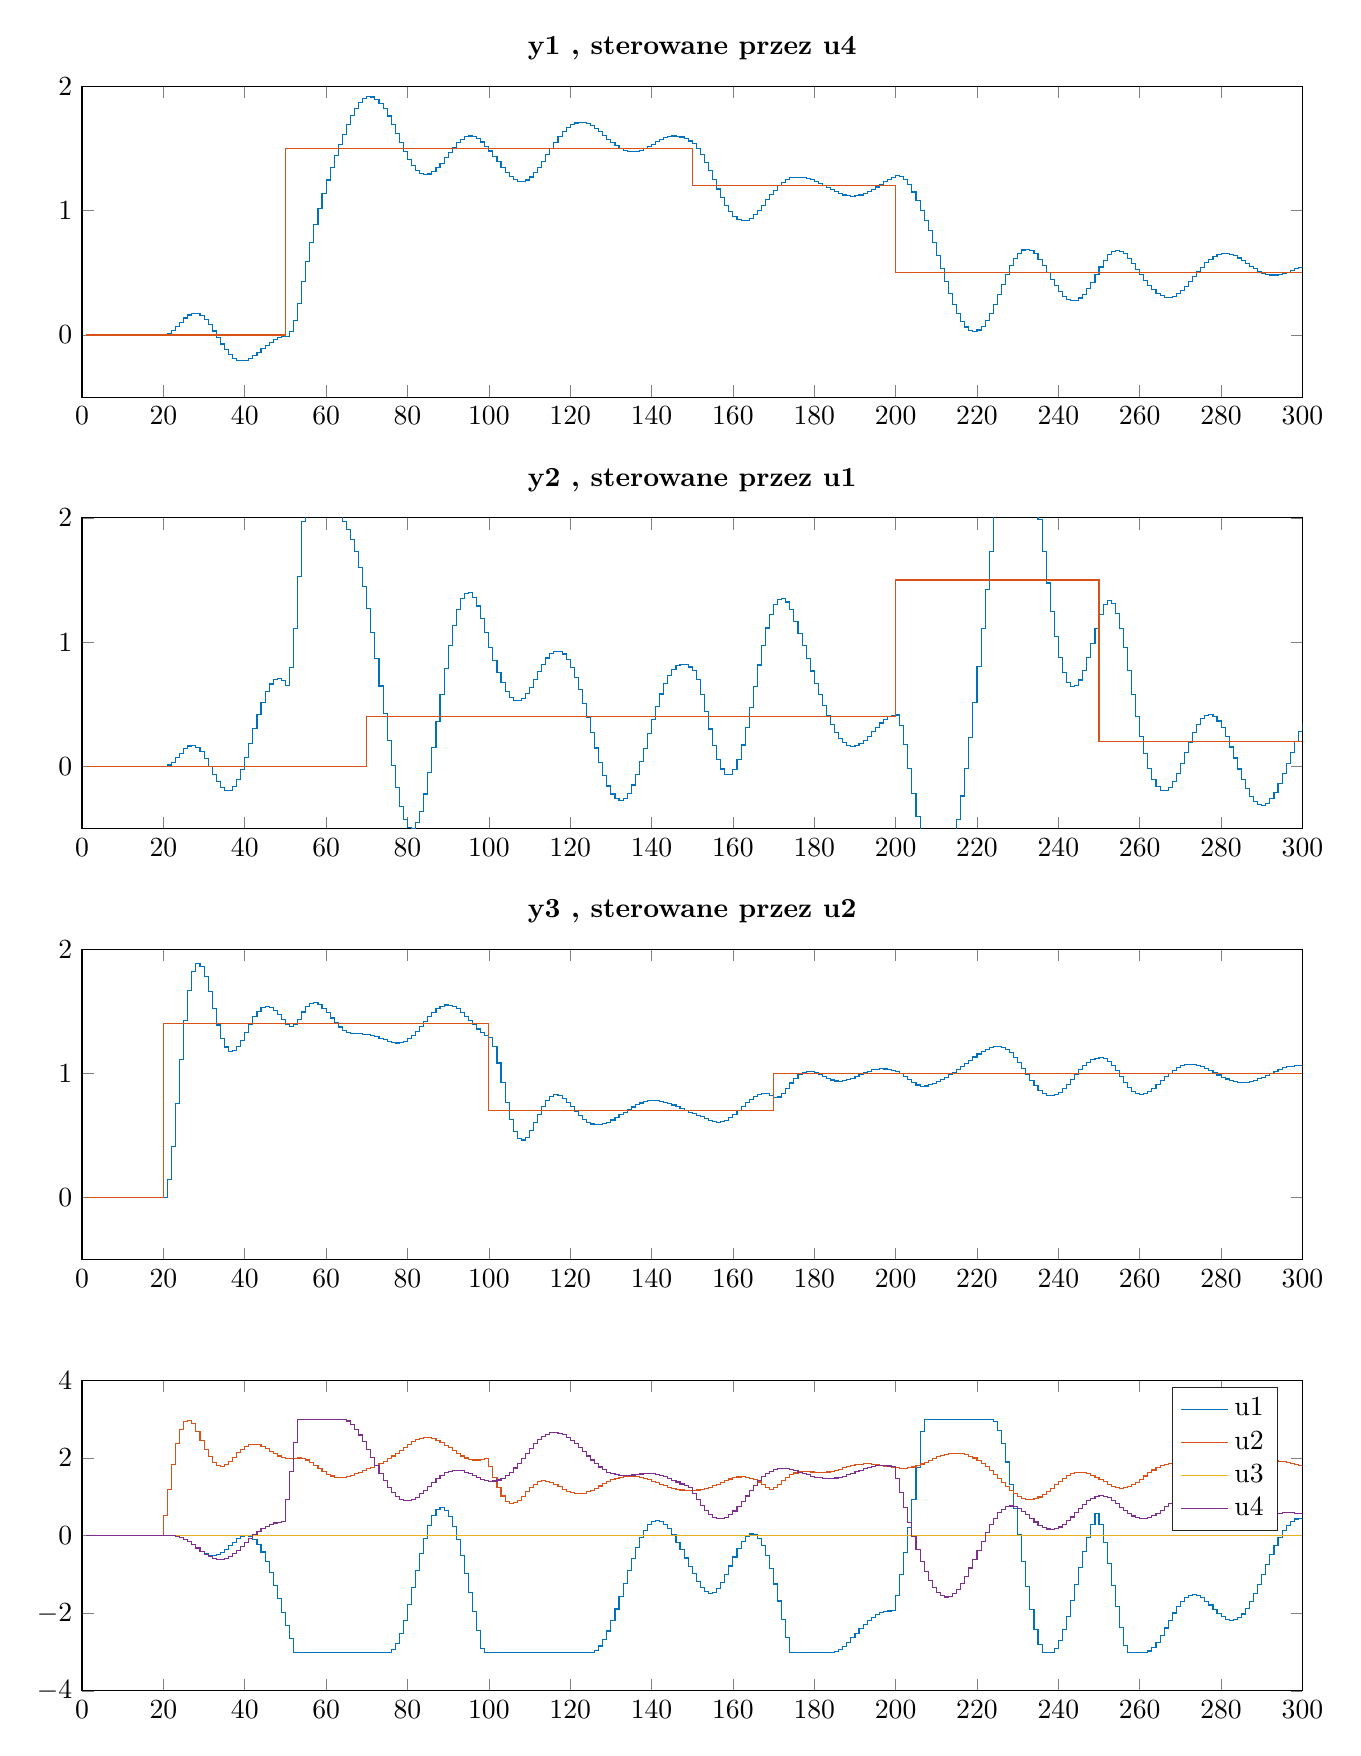
\begin{tikzpicture}

\begin{axis}[%
width=6.102in,
height=1.553in,
at={(1.024in,7.552in)},
scale only axis,
xmin=0,
xmax=300,
ymin=-0.5,
ymax=2,
axis background/.style={fill=white},
title style={font=\bfseries},
title={y1 , sterowane przez u4}
]
\addplot[const plot, color=mycolor1, forget plot] table[row sep=crcr] {%
1	0\\
2	0\\
3	0\\
4	0\\
5	0\\
6	0\\
7	0\\
8	0\\
9	0\\
10	0\\
11	0\\
12	0\\
13	0\\
14	0\\
15	0\\
16	0\\
17	0\\
18	0\\
19	0\\
20	0\\
21	0.0114581194369012\\
22	0.0352462992044872\\
23	0.0676907939762602\\
24	0.103284682890995\\
25	0.136157218461565\\
26	0.160961771971097\\
27	0.173593551447536\\
28	0.171640498218183\\
29	0.154552086192241\\
30	0.123550320641774\\
31	0.0813341331811921\\
32	0.0316445153011482\\
33	-0.0212371701454259\\
34	-0.0729897296893186\\
35	-0.119695233332739\\
36	-0.158184462523214\\
37	-0.186262280020865\\
38	-0.202807513431365\\
39	-0.207756385786551\\
40	-0.201989228248191\\
41	-0.187146695655913\\
42	-0.165404096992787\\
43	-0.139231329151075\\
44	-0.111162132752843\\
45	-0.0835909640614092\\
46	-0.058609662479981\\
47	-0.037890116161352\\
48	-0.0226139078516852\\
49	-0.0134458412181265\\
50	-0.0105454573156293\\
51	0.0301043646509756\\
52	0.119553157004102\\
53	0.255749611126188\\
54	0.431102098795633\\
55	0.594655960469464\\
56	0.746574770334774\\
57	0.887170284996476\\
58	1.01698014024325\\
59	1.13674779481489\\
60	1.24736126641489\\
61	1.34977716419261\\
62	1.44494431030253\\
63	1.53373839644912\\
64	1.61691494792168\\
65	1.69481410932536\\
66	1.76456817243396\\
67	1.82358677554655\\
68	1.86964986973855\\
69	1.90102242349027\\
70	1.91655130402287\\
71	1.91573041607831\\
72	1.89872949623064\\
73	1.8663853628059\\
74	1.8201576058604\\
75	1.76205326061254\\
76	1.69452678861324\\
77	1.62137734390821\\
78	1.5472506580497\\
79	1.47662075754823\\
80	1.41352250355594\\
81	1.36130912592551\\
82	1.32246277605679\\
83	1.29847126431886\\
84	1.28977655429641\\
85	1.29579498015894\\
86	1.31500402950822\\
87	1.34508625391606\\
88	1.38311763287972\\
89	1.42578562425516\\
90	1.46962119743605\\
91	1.51122930080394\\
92	1.54750333881102\\
93	1.57581116063595\\
94	1.59414259995046\\
95	1.60121155086978\\
96	1.59650871626906\\
97	1.58030432921909\\
98	1.55360315173201\\
99	1.51805674561835\\
100	1.48102921101008\\
101	1.43979246800295\\
102	1.39527136407394\\
103	1.35042942753239\\
104	1.30884983393925\\
105	1.27400084032942\\
106	1.24882538513035\\
107	1.23543321233677\\
108	1.23493089792199\\
109	1.24738644264181\\
110	1.27190866398633\\
111	1.30681212871988\\
112	1.34983418239383\\
113	1.39837136493807\\
114	1.44970704536736\\
115	1.50120909754692\\
116	1.55048447976536\\
117	1.59548543694455\\
118	1.63456876246733\\
119	1.66651453129309\\
120	1.69051369553788\\
121	1.70613497922433\\
122	1.71328092156083\\
123	1.7121411497407\\
124	1.70314852499099\\
125	1.6869411920652\\
126	1.66433118469719\\
127	1.63705283869518\\
128	1.60715999578642\\
129	1.57671752835371\\
130	1.54768964056372\\
131	1.52183172066941\\
132	1.50059608129961\\
133	1.48505739386617\\
134	1.47586198871333\\
135	1.47320375823764\\
136	1.47682775756149\\
137	1.48606086776544\\
138	1.49986718824609\\
139	1.51692427923993\\
140	1.53571509589991\\
141	1.55462953398554\\
142	1.57206900766988\\
143	1.58654743157885\\
144	1.59678237590082\\
145	1.60177096563829\\
146	1.60084623443044\\
147	1.59371102952633\\
148	1.58044809331381\\
149	1.56150650900354\\
150	1.53766618747092\\
151	1.5012406982206\\
152	1.451423809674\\
153	1.39033014763567\\
154	1.32129118321007\\
155	1.24815168656435\\
156	1.17496775974125\\
157	1.10570434162766\\
158	1.04396087285235\\
159	0.992740193668317\\
160	0.954272291977563\\
161	0.929900913491391\\
162	0.920036567928608\\
163	0.924174832043229\\
164	0.94097455265276\\
165	0.968386937657526\\
166	1.00382381016951\\
167	1.04435159766729\\
168	1.08689694705353\\
169	1.12845013470871\\
170	1.16625355965338\\
171	1.20041972381471\\
172	1.22933570598056\\
173	1.25104543828875\\
174	1.26387531995352\\
175	1.26823760644317\\
176	1.2694560735235\\
177	1.26703628801114\\
178	1.26083767101717\\
179	1.25102469114311\\
180	1.23803550961222\\
181	1.22253397447472\\
182	1.20534389773312\\
183	1.18737558286595\\
184	1.16955334617862\\
185	1.15275097716991\\
186	1.13808774058987\\
187	1.12671045789807\\
188	1.11948452873852\\
189	1.11695651825058\\
190	1.11933696796097\\
191	1.12650655612185\\
192	1.1380436289577\\
193	1.15326926159667\\
194	1.17130526531894\\
195	1.19114024790575\\
196	1.21169890257993\\
197	1.23191006265038\\
198	1.25076962845449\\
199	1.26739517482919\\
200	1.28106981850292\\
201	1.2775456187648\\
202	1.25345395882948\\
203	1.21013673363028\\
204	1.15100597114401\\
205	1.08045858243762\\
206	1.00342664828425\\
207	0.924933624865126\\
208	0.838422560864861\\
209	0.742266146625648\\
210	0.640134356808953\\
211	0.535813830111922\\
212	0.433137239527689\\
213	0.3358470747477\\
214	0.24745134575343\\
215	0.171087307289292\\
216	0.109400152108603\\
217	0.0644428546050118\\
218	0.0376019381082947\\
219	0.0295522893770994\\
220	0.0402424257643971\\
221	0.0689099693254966\\
222	0.114125603735592\\
223	0.173862555470815\\
224	0.245587687521727\\
225	0.325267443515469\\
226	0.407312825676907\\
227	0.48627091506028\\
228	0.557141273454691\\
229	0.615677922923046\\
230	0.65863639647986\\
231	0.683946539190217\\
232	0.690801643076305\\
233	0.679661098419947\\
234	0.652170106307822\\
235	0.611005596112695\\
236	0.559662011115219\\
237	0.503759987620358\\
238	0.448525446752281\\
239	0.396035902206359\\
240	0.349668188334709\\
241	0.312676511383758\\
242	0.287622175633422\\
243	0.276255526093334\\
244	0.279441344106768\\
245	0.297138929226362\\
246	0.32843662510736\\
247	0.371636498265592\\
248	0.424382159069538\\
249	0.483820471342543\\
250	0.546786276620044\\
251	0.60211379987115\\
252	0.644515265640234\\
253	0.671360750752936\\
254	0.681482705924961\\
255	0.674854857190243\\
256	0.652562326880637\\
257	0.616684309939892\\
258	0.57391973919687\\
259	0.528935624088913\\
260	0.483654969202943\\
261	0.439883097296913\\
262	0.399218756237845\\
263	0.363470350454534\\
264	0.334731568060066\\
265	0.314582186530237\\
266	0.304041199500674\\
267	0.303539272301767\\
268	0.312921138206462\\
269	0.331478843607498\\
270	0.358013438889892\\
271	0.390921306892299\\
272	0.428300013442345\\
273	0.468067498314288\\
274	0.508087682572197\\
275	0.546295216536396\\
276	0.580812175931716\\
277	0.610050044955848\\
278	0.6327912812361\\
279	0.648246080986868\\
280	0.656081564615444\\
281	0.656422372181411\\
282	0.649823470129029\\
283	0.637217698989906\\
284	0.619842118013199\\
285	0.599148426257876\\
286	0.576703584831835\\
287	0.554087185670374\\
288	0.532792094329916\\
289	0.514134454843952\\
290	0.499178329246886\\
291	0.488679121981031\\
292	0.48304859649206\\
293	0.482342824708649\\
294	0.486272919825052\\
295	0.494236985249903\\
296	0.505370454402441\\
297	0.518610969143818\\
298	0.532773202523142\\
299	0.546628607023813\\
300	0.558984973968527\\
};
\addplot[const plot, color=mycolor2, forget plot] table[row sep=crcr] {%
1	0\\
2	0\\
3	0\\
4	0\\
5	0\\
6	0\\
7	0\\
8	0\\
9	0\\
10	0\\
11	0\\
12	0\\
13	0\\
14	0\\
15	0\\
16	0\\
17	0\\
18	0\\
19	0\\
20	0\\
21	0\\
22	0\\
23	0\\
24	0\\
25	0\\
26	0\\
27	0\\
28	0\\
29	0\\
30	0\\
31	0\\
32	0\\
33	0\\
34	0\\
35	0\\
36	0\\
37	0\\
38	0\\
39	0\\
40	0\\
41	0\\
42	0\\
43	0\\
44	0\\
45	0\\
46	0\\
47	0\\
48	0\\
49	0\\
50	1.5\\
51	1.5\\
52	1.5\\
53	1.5\\
54	1.5\\
55	1.5\\
56	1.5\\
57	1.5\\
58	1.5\\
59	1.5\\
60	1.5\\
61	1.5\\
62	1.5\\
63	1.5\\
64	1.5\\
65	1.5\\
66	1.5\\
67	1.5\\
68	1.5\\
69	1.5\\
70	1.5\\
71	1.5\\
72	1.5\\
73	1.5\\
74	1.5\\
75	1.5\\
76	1.5\\
77	1.5\\
78	1.5\\
79	1.5\\
80	1.5\\
81	1.5\\
82	1.5\\
83	1.5\\
84	1.5\\
85	1.5\\
86	1.5\\
87	1.5\\
88	1.5\\
89	1.5\\
90	1.5\\
91	1.5\\
92	1.5\\
93	1.5\\
94	1.5\\
95	1.5\\
96	1.5\\
97	1.5\\
98	1.5\\
99	1.5\\
100	1.5\\
101	1.5\\
102	1.5\\
103	1.5\\
104	1.5\\
105	1.5\\
106	1.5\\
107	1.5\\
108	1.5\\
109	1.5\\
110	1.5\\
111	1.5\\
112	1.5\\
113	1.5\\
114	1.5\\
115	1.5\\
116	1.5\\
117	1.5\\
118	1.5\\
119	1.5\\
120	1.5\\
121	1.5\\
122	1.5\\
123	1.5\\
124	1.5\\
125	1.5\\
126	1.5\\
127	1.5\\
128	1.5\\
129	1.5\\
130	1.5\\
131	1.5\\
132	1.5\\
133	1.5\\
134	1.5\\
135	1.5\\
136	1.5\\
137	1.5\\
138	1.5\\
139	1.5\\
140	1.5\\
141	1.5\\
142	1.5\\
143	1.5\\
144	1.5\\
145	1.5\\
146	1.5\\
147	1.5\\
148	1.5\\
149	1.5\\
150	1.2\\
151	1.2\\
152	1.2\\
153	1.2\\
154	1.2\\
155	1.2\\
156	1.2\\
157	1.2\\
158	1.2\\
159	1.2\\
160	1.2\\
161	1.2\\
162	1.2\\
163	1.2\\
164	1.2\\
165	1.2\\
166	1.2\\
167	1.2\\
168	1.2\\
169	1.2\\
170	1.2\\
171	1.2\\
172	1.2\\
173	1.2\\
174	1.2\\
175	1.2\\
176	1.2\\
177	1.2\\
178	1.2\\
179	1.2\\
180	1.2\\
181	1.2\\
182	1.2\\
183	1.2\\
184	1.2\\
185	1.2\\
186	1.2\\
187	1.2\\
188	1.2\\
189	1.2\\
190	1.2\\
191	1.2\\
192	1.2\\
193	1.2\\
194	1.2\\
195	1.2\\
196	1.2\\
197	1.2\\
198	1.2\\
199	1.2\\
200	0.5\\
201	0.5\\
202	0.5\\
203	0.5\\
204	0.5\\
205	0.5\\
206	0.5\\
207	0.5\\
208	0.5\\
209	0.5\\
210	0.5\\
211	0.5\\
212	0.5\\
213	0.5\\
214	0.5\\
215	0.5\\
216	0.5\\
217	0.5\\
218	0.5\\
219	0.5\\
220	0.5\\
221	0.5\\
222	0.5\\
223	0.5\\
224	0.5\\
225	0.5\\
226	0.5\\
227	0.5\\
228	0.5\\
229	0.5\\
230	0.5\\
231	0.5\\
232	0.5\\
233	0.5\\
234	0.5\\
235	0.5\\
236	0.5\\
237	0.5\\
238	0.5\\
239	0.5\\
240	0.5\\
241	0.5\\
242	0.5\\
243	0.5\\
244	0.5\\
245	0.5\\
246	0.5\\
247	0.5\\
248	0.5\\
249	0.5\\
250	0.5\\
251	0.5\\
252	0.5\\
253	0.5\\
254	0.5\\
255	0.5\\
256	0.5\\
257	0.5\\
258	0.5\\
259	0.5\\
260	0.5\\
261	0.5\\
262	0.5\\
263	0.5\\
264	0.5\\
265	0.5\\
266	0.5\\
267	0.5\\
268	0.5\\
269	0.5\\
270	0.5\\
271	0.5\\
272	0.5\\
273	0.5\\
274	0.5\\
275	0.5\\
276	0.5\\
277	0.5\\
278	0.5\\
279	0.5\\
280	0.5\\
281	0.5\\
282	0.5\\
283	0.5\\
284	0.5\\
285	0.5\\
286	0.5\\
287	0.5\\
288	0.5\\
289	0.5\\
290	0.5\\
291	0.5\\
292	0.5\\
293	0.5\\
294	0.5\\
295	0.5\\
296	0.5\\
297	0.5\\
298	0.5\\
299	0.5\\
300	0.5\\
};
\end{axis}

\begin{axis}[%
width=6.102in,
height=1.553in,
at={(1.024in,5.395in)},
scale only axis,
xmin=0,
xmax=300,
ymin=-0.5,
ymax=2,
axis background/.style={fill=white},
title style={font=\bfseries},
title={y2 , sterowane przez u1}
]
\addplot[const plot, color=mycolor1, forget plot] table[row sep=crcr] {%
1	0\\
2	0\\
3	0\\
4	0\\
5	0\\
6	0\\
7	0\\
8	0\\
9	0\\
10	0\\
11	0\\
12	0\\
13	0\\
14	0\\
15	0\\
16	0\\
17	0\\
18	0\\
19	0\\
20	0\\
21	0.0105699306087332\\
22	0.0344208390223349\\
23	0.0687294577653415\\
24	0.10701016479669\\
25	0.14120710006361\\
26	0.163584135392296\\
27	0.168290280708304\\
28	0.152386882056316\\
29	0.11627964595281\\
30	0.0635879140547024\\
31	0.000550205858596595\\
32	-0.0648912368132751\\
33	-0.124165558278763\\
34	-0.169151105806222\\
35	-0.193121829716848\\
36	-0.191463366710609\\
37	-0.16210112148034\\
38	-0.105623919208735\\
39	-0.0251232581692377\\
40	0.074203518309434\\
41	0.185619458962414\\
42	0.301508842956124\\
43	0.414058939747156\\
44	0.515897580323338\\
45	0.60063513756387\\
46	0.663275943174398\\
47	0.700481095146167\\
48	0.71068021571309\\
49	0.694042716933413\\
50	0.652328790697623\\
51	0.796103159695599\\
52	1.10956231088044\\
53	1.5266640556255\\
54	1.97124375266084\\
55	2.20539698289038\\
56	2.31303883411041\\
57	2.34485375358609\\
58	2.33151243137397\\
59	2.29165049928346\\
60	2.23667448335447\\
61	2.17364409294161\\
62	2.10698888782606\\
63	2.03952335745318\\
64	1.97304425720301\\
65	1.90740383998202\\
66	1.82791813531366\\
67	1.72663854935612\\
68	1.60005707210248\\
69	1.44782835822416\\
70	1.2719690109101\\
71	1.07629575441786\\
72	0.865984660304771\\
73	0.64718522162044\\
74	0.426656539744965\\
75	0.211414028314087\\
76	0.00838779964060321\\
77	-0.172880207768515\\
78	-0.321678896643674\\
79	-0.429090848486239\\
80	-0.488631553004644\\
81	-0.496711226449357\\
82	-0.452860586240211\\
83	-0.359721049072171\\
84	-0.222818148468042\\
85	-0.0501469061998\\
86	0.148392664774358\\
87	0.36166453595785\\
88	0.578020571324212\\
89	0.786029042128144\\
90	0.975159961562067\\
91	1.13638495758079\\
92	1.2626573147549\\
93	1.34924744652548\\
94	1.39391965922847\\
95	1.39694689203839\\
96	1.3609704675405\\
97	1.29072116085244\\
98	1.19262560253941\\
99	1.07432781611933\\
100	0.959597890380926\\
101	0.852721381805609\\
102	0.755801388186141\\
103	0.672048027631944\\
104	0.605010808922088\\
105	0.55783134109992\\
106	0.532615259114162\\
107	0.529960275788371\\
108	0.548727069280338\\
109	0.586059194265966\\
110	0.637619450505516\\
111	0.697986584349662\\
112	0.761144793443373\\
113	0.820998180573758\\
114	0.871850649475546\\
115	0.908805836566232\\
116	0.928058543821186\\
117	0.927066093614813\\
118	0.904602944844113\\
119	0.860713378638868\\
120	0.796584406052807\\
121	0.714364260620927\\
122	0.616951433394001\\
123	0.507776053216982\\
124	0.390590539426161\\
125	0.269280881303841\\
126	0.147704514515417\\
127	0.0318604258056879\\
128	-0.0719805580752591\\
129	-0.158250974678544\\
130	-0.222420571624301\\
131	-0.261252177735791\\
132	-0.272959356449274\\
133	-0.257266170419701\\
134	-0.215373666017098\\
135	-0.149840594819531\\
136	-0.0643893059955374\\
137	0.0363489609258136\\
138	0.147132384359396\\
139	0.262431528727369\\
140	0.3767571205847\\
141	0.484973014667278\\
142	0.582576125570204\\
143	0.665927579297409\\
144	0.732422743378053\\
145	0.780591897221732\\
146	0.810127829196951\\
147	0.821841290132568\\
148	0.817549688155258\\
149	0.799908390601663\\
150	0.772197259191974\\
151	0.696586053484007\\
152	0.580850674065952\\
153	0.443150268334125\\
154	0.300886145345819\\
155	0.168526559459213\\
156	0.0579602515245445\\
157	-0.0215486401817033\\
158	-0.0635203800056063\\
159	-0.0643958205790553\\
160	-0.0235710222035704\\
161	0.0567095998780868\\
162	0.171613247012334\\
163	0.314122391386783\\
164	0.475557306837183\\
165	0.646182253446851\\
166	0.815854154396231\\
167	0.974670714543433\\
168	1.11357660180036\\
169	1.2248909609148\\
170	1.30272648723816\\
171	1.34554382190512\\
172	1.35235045385531\\
173	1.32320306208542\\
174	1.25947603086258\\
175	1.16848270590377\\
176	1.07141857154507\\
177	0.970863211462982\\
178	0.869069215184701\\
179	0.768001727263683\\
180	0.669507921972172\\
181	0.575391337544802\\
182	0.487385959773938\\
183	0.407078447532836\\
184	0.335812972028723\\
185	0.274602877263944\\
186	0.22509977849968\\
187	0.18900282470943\\
188	0.16717892071877\\
189	0.159597776627822\\
190	0.165341026425439\\
191	0.182688877151615\\
192	0.209268474800216\\
193	0.242244770494322\\
194	0.278534975218104\\
195	0.315028650209555\\
196	0.348797261429412\\
197	0.37727952449409\\
198	0.398431880860981\\
199	0.410836745942587\\
200	0.413764529527441\\
201	0.330225143053215\\
202	0.175109044124065\\
203	-0.0179403741337654\\
204	-0.218424412073982\\
205	-0.402250768141027\\
206	-0.550123956844183\\
207	-0.64700557953975\\
208	-0.71556771654205\\
209	-0.76558599445315\\
210	-0.791902514978041\\
211	-0.78962310685202\\
212	-0.754411126580171\\
213	-0.682938408076317\\
214	-0.573210399339718\\
215	-0.424754460221318\\
216	-0.238698709852133\\
217	-0.0177577445164112\\
218	0.233862811764453\\
219	0.510632083605959\\
220	0.805918697437364\\
221	1.1122620121355\\
222	1.42167617809617\\
223	1.72597260940793\\
224	2.0170862691608\\
225	2.2841123206942\\
226	2.51312978741311\\
227	2.69221792139374\\
228	2.81227183527888\\
229	2.86763321786478\\
230	2.8564390019456\\
231	2.7806821597724\\
232	2.64600463712686\\
233	2.46125310600081\\
234	2.23783961139026\\
235	1.98895871762434\\
236	1.72871912619881\\
237	1.47590994195515\\
238	1.24640526630013\\
239	1.0450244558535\\
240	0.87910689286895\\
241	0.754633976171689\\
242	0.674847427992357\\
243	0.640196349822838\\
244	0.648428193359595\\
245	0.694849667644569\\
246	0.772732385709406\\
247	0.873828338658747\\
248	0.988956993337647\\
249	1.10862413158519\\
250	1.22363294162772\\
251	1.3021917140709\\
252	1.33149005867723\\
253	1.30799467222891\\
254	1.23339364805629\\
255	1.11298639019486\\
256	0.955012448992388\\
257	0.769862497033323\\
258	0.580561215960052\\
259	0.402611284185978\\
260	0.241773234280538\\
261	0.102124021995114\\
262	-0.0138439315574027\\
263	-0.103657397383173\\
264	-0.164412745611358\\
265	-0.195007559411549\\
266	-0.196134421768154\\
267	-0.170189874190879\\
268	-0.121072898161275\\
269	-0.0538922896592306\\
270	0.0253896764002908\\
271	0.110350903234106\\
272	0.194514836599424\\
273	0.271743204343112\\
274	0.336593842570963\\
275	0.384624213698021\\
276	0.412624943385666\\
277	0.418772137749808\\
278	0.402692196857178\\
279	0.365438063766553\\
280	0.309381050227147\\
281	0.238027255997292\\
282	0.155771854343485\\
283	0.0676078919535285\\
284	-0.0211914565845671\\
285	-0.105397163005749\\
286	-0.180135319453258\\
287	-0.241166399383506\\
288	-0.285116917395313\\
289	-0.309651044125395\\
290	-0.313573848225362\\
291	-0.296862340536054\\
292	-0.260625084787061\\
293	-0.206995518169794\\
294	-0.138968022432923\\
295	-0.0601889721934609\\
296	0.0252827121879021\\
297	0.113229674372881\\
298	0.1995287928311\\
299	0.280387052469187\\
300	0.352546919595404\\
};
\addplot[const plot, color=mycolor2, forget plot] table[row sep=crcr] {%
1	0\\
2	0\\
3	0\\
4	0\\
5	0\\
6	0\\
7	0\\
8	0\\
9	0\\
10	0\\
11	0\\
12	0\\
13	0\\
14	0\\
15	0\\
16	0\\
17	0\\
18	0\\
19	0\\
20	0\\
21	0\\
22	0\\
23	0\\
24	0\\
25	0\\
26	0\\
27	0\\
28	0\\
29	0\\
30	0\\
31	0\\
32	0\\
33	0\\
34	0\\
35	0\\
36	0\\
37	0\\
38	0\\
39	0\\
40	0\\
41	0\\
42	0\\
43	0\\
44	0\\
45	0\\
46	0\\
47	0\\
48	0\\
49	0\\
50	0\\
51	0\\
52	0\\
53	0\\
54	0\\
55	0\\
56	0\\
57	0\\
58	0\\
59	0\\
60	0\\
61	0\\
62	0\\
63	0\\
64	0\\
65	0\\
66	0\\
67	0\\
68	0\\
69	0\\
70	0.4\\
71	0.4\\
72	0.4\\
73	0.4\\
74	0.4\\
75	0.4\\
76	0.4\\
77	0.4\\
78	0.4\\
79	0.4\\
80	0.4\\
81	0.4\\
82	0.4\\
83	0.4\\
84	0.4\\
85	0.4\\
86	0.4\\
87	0.4\\
88	0.4\\
89	0.4\\
90	0.4\\
91	0.4\\
92	0.4\\
93	0.4\\
94	0.4\\
95	0.4\\
96	0.4\\
97	0.4\\
98	0.4\\
99	0.4\\
100	0.4\\
101	0.4\\
102	0.4\\
103	0.4\\
104	0.4\\
105	0.4\\
106	0.4\\
107	0.4\\
108	0.4\\
109	0.4\\
110	0.4\\
111	0.4\\
112	0.4\\
113	0.4\\
114	0.4\\
115	0.4\\
116	0.4\\
117	0.4\\
118	0.4\\
119	0.4\\
120	0.4\\
121	0.4\\
122	0.4\\
123	0.4\\
124	0.4\\
125	0.4\\
126	0.4\\
127	0.4\\
128	0.4\\
129	0.4\\
130	0.4\\
131	0.4\\
132	0.4\\
133	0.4\\
134	0.4\\
135	0.4\\
136	0.4\\
137	0.4\\
138	0.4\\
139	0.4\\
140	0.4\\
141	0.4\\
142	0.4\\
143	0.4\\
144	0.4\\
145	0.4\\
146	0.4\\
147	0.4\\
148	0.4\\
149	0.4\\
150	0.4\\
151	0.4\\
152	0.4\\
153	0.4\\
154	0.4\\
155	0.4\\
156	0.4\\
157	0.4\\
158	0.4\\
159	0.4\\
160	0.4\\
161	0.4\\
162	0.4\\
163	0.4\\
164	0.4\\
165	0.4\\
166	0.4\\
167	0.4\\
168	0.4\\
169	0.4\\
170	0.4\\
171	0.4\\
172	0.4\\
173	0.4\\
174	0.4\\
175	0.4\\
176	0.4\\
177	0.4\\
178	0.4\\
179	0.4\\
180	0.4\\
181	0.4\\
182	0.4\\
183	0.4\\
184	0.4\\
185	0.4\\
186	0.4\\
187	0.4\\
188	0.4\\
189	0.4\\
190	0.4\\
191	0.4\\
192	0.4\\
193	0.4\\
194	0.4\\
195	0.4\\
196	0.4\\
197	0.4\\
198	0.4\\
199	0.4\\
200	1.5\\
201	1.5\\
202	1.5\\
203	1.5\\
204	1.5\\
205	1.5\\
206	1.5\\
207	1.5\\
208	1.5\\
209	1.5\\
210	1.5\\
211	1.5\\
212	1.5\\
213	1.5\\
214	1.5\\
215	1.5\\
216	1.5\\
217	1.5\\
218	1.5\\
219	1.5\\
220	1.5\\
221	1.5\\
222	1.5\\
223	1.5\\
224	1.5\\
225	1.5\\
226	1.5\\
227	1.5\\
228	1.5\\
229	1.5\\
230	1.5\\
231	1.5\\
232	1.5\\
233	1.5\\
234	1.5\\
235	1.5\\
236	1.5\\
237	1.5\\
238	1.5\\
239	1.5\\
240	1.5\\
241	1.5\\
242	1.5\\
243	1.5\\
244	1.5\\
245	1.5\\
246	1.5\\
247	1.5\\
248	1.5\\
249	1.5\\
250	0.2\\
251	0.2\\
252	0.2\\
253	0.2\\
254	0.2\\
255	0.2\\
256	0.2\\
257	0.2\\
258	0.2\\
259	0.2\\
260	0.2\\
261	0.2\\
262	0.2\\
263	0.2\\
264	0.2\\
265	0.2\\
266	0.2\\
267	0.2\\
268	0.2\\
269	0.2\\
270	0.2\\
271	0.2\\
272	0.2\\
273	0.2\\
274	0.2\\
275	0.2\\
276	0.2\\
277	0.2\\
278	0.2\\
279	0.2\\
280	0.2\\
281	0.2\\
282	0.2\\
283	0.2\\
284	0.2\\
285	0.2\\
286	0.2\\
287	0.2\\
288	0.2\\
289	0.2\\
290	0.2\\
291	0.2\\
292	0.2\\
293	0.2\\
294	0.2\\
295	0.2\\
296	0.2\\
297	0.2\\
298	0.2\\
299	0.2\\
300	0.2\\
};
\end{axis}

\begin{axis}[%
width=6.102in,
height=1.553in,
at={(1.024in,3.239in)},
scale only axis,
xmin=0,
xmax=300,
ymin=-0.5,
ymax=2,
axis background/.style={fill=white},
title style={font=\bfseries},
title={y3 , sterowane przez u2}
]
\addplot[const plot, color=mycolor1, forget plot] table[row sep=crcr] {%
1	0\\
2	0\\
3	0\\
4	0\\
5	0\\
6	0\\
7	0\\
8	0\\
9	0\\
10	0\\
11	0\\
12	0\\
13	0\\
14	0\\
15	0\\
16	0\\
17	0\\
18	0\\
19	0\\
20	0\\
21	0.142671982788199\\
22	0.414294892302412\\
23	0.757102785849964\\
24	1.11054859176318\\
25	1.42560327325309\\
26	1.66828904126256\\
27	1.82103922646889\\
28	1.88169254904896\\
29	1.86070004657478\\
30	1.77726313383914\\
31	1.65510917396648\\
32	1.5185162096633\\
33	1.38904511389189\\
34	1.28325654157452\\
35	1.21151013841184\\
36	1.17778706147305\\
37	1.18035905338856\\
38	1.21305524862547\\
39	1.26685151889862\\
40	1.33152066993341\\
41	1.3971255049262\\
42	1.45519913017058\\
43	1.4995263247527\\
44	1.52650619497272\\
45	1.53513197648616\\
46	1.52666393183294\\
47	1.5040939415587\\
48	1.4715062960416\\
49	1.43343101562672\\
50	1.39426763999697\\
51	1.37913386480171\\
52	1.39402683655479\\
53	1.43505828746532\\
54	1.4933197007574\\
55	1.5371594912553\\
56	1.56205606596352\\
57	1.56655180171187\\
58	1.55244156740839\\
59	1.52388963760809\\
60	1.48633006783335\\
61	1.44545109051821\\
62	1.40636698503268\\
63	1.37304426474835\\
64	1.34800242982743\\
65	1.33213828762579\\
66	1.32354186978937\\
67	1.31964138143851\\
68	1.31772601488461\\
69	1.31543293983794\\
70	1.31108953712565\\
71	1.30388472429564\\
72	1.29388009575559\\
73	1.28188974665238\\
74	1.26926925455745\\
75	1.25765841525176\\
76	1.24871989728054\\
77	1.24450215454382\\
78	1.2470502456255\\
79	1.25772610744731\\
80	1.27700643343404\\
81	1.30439540203098\\
82	1.33846892469211\\
83	1.37703374636713\\
84	1.41737049551749\\
85	1.45652392787545\\
86	1.49160278062931\\
87	1.52005531816659\\
88	1.53989362391855\\
89	1.54984861026045\\
90	1.54944724260035\\
91	1.53901244579483\\
92	1.51959370130662\\
93	1.49284189904914\\
94	1.46084535070963\\
95	1.42594505882741\\
96	1.39054664530778\\
97	1.35694419417016\\
98	1.32716814092497\\
99	1.3028657266123\\
100	1.28825411708241\\
101	1.21295129876325\\
102	1.08289719892021\\
103	0.925140186960836\\
104	0.767524504664203\\
105	0.63192034761018\\
106	0.532803169586473\\
107	0.476845161712842\\
108	0.463593784817429\\
109	0.486941804006021\\
110	0.537037069488416\\
111	0.602297211621788\\
112	0.671248682178672\\
113	0.733988903523593\\
114	0.783159395022915\\
115	0.814403169909034\\
116	0.826351204417336\\
117	0.820234014027229\\
118	0.799242871173884\\
119	0.767771931262878\\
120	0.730661068300057\\
121	0.692534740368871\\
122	0.657300508761742\\
123	0.627837468466016\\
124	0.605874441126394\\
125	0.592033638196477\\
126	0.58599944471868\\
127	0.587217423673722\\
128	0.594833079658719\\
129	0.607746974444754\\
130	0.624737780648214\\
131	0.644552553676325\\
132	0.665970953463131\\
133	0.687847499281441\\
134	0.709137475611086\\
135	0.728912732805277\\
136	0.746372907735849\\
137	0.760856013679247\\
138	0.771850364220512\\
139	0.779007822357274\\
140	0.782156742434826\\
141	0.781311924740406\\
142	0.776678531578273\\
143	0.76864720327563\\
144	0.757778451132238\\
145	0.744775615071948\\
146	0.730447048678002\\
147	0.715659526350953\\
148	0.701285977271054\\
149	0.688151406277341\\
150	0.676981187396369\\
151	0.664095662951699\\
152	0.649282594033979\\
153	0.633962671364824\\
154	0.620295092307571\\
155	0.610595193321262\\
156	0.606918254784969\\
157	0.610709189816473\\
158	0.622571755975401\\
159	0.642174244432204\\
160	0.668287737013609\\
161	0.698937064384986\\
162	0.731633499074578\\
163	0.76365264070168\\
164	0.792320608799942\\
165	0.815275680861032\\
166	0.830679669758067\\
167	0.837362252974775\\
168	0.834890823418431\\
169	0.823567103210782\\
170	0.804358914863226\\
171	0.809353205250035\\
172	0.837516288616342\\
173	0.878596506213805\\
174	0.92179331968054\\
175	0.959531579896975\\
176	0.989652482794745\\
177	1.00921178117056\\
178	1.01749642834294\\
179	1.01554988206939\\
180	1.00566095646181\\
181	0.990809219578581\\
182	0.974129620924218\\
183	0.958463119154924\\
184	0.946034052916357\\
185	0.938270451337968\\
186	0.935965387595531\\
187	0.939245617132034\\
188	0.947541884285324\\
189	0.959749499305699\\
190	0.974421804626689\\
191	0.989973956226571\\
192	1.00487248852312\\
193	1.01779149673129\\
194	1.02772365444105\\
195	1.03404155159141\\
196	1.03651121753703\\
197	1.0352646082634\\
198	1.0307410024379\\
199	1.02360865599977\\
200	1.01467791320641\\
201	0.998777796298947\\
202	0.976379110531614\\
203	0.950612608891241\\
204	0.925776854211572\\
205	0.906343968993828\\
206	0.896247603130073\\
207	0.898309489981514\\
208	0.907287356125568\\
209	0.919567962009428\\
210	0.934251752200878\\
211	0.950731701323399\\
212	0.968752472768135\\
213	0.988290191165713\\
214	1.00940180458986\\
215	1.03208673153652\\
216	1.05617940754099\\
217	1.08128496996805\\
218	1.10676217392202\\
219	1.13175041769538\\
220	1.1552322765572\\
221	1.17611955715132\\
222	1.19334962394707\\
223	1.20597936987168\\
224	1.21326627129448\\
225	1.21408423100995\\
226	1.206853467447\\
227	1.19052132986007\\
228	1.1647792330458\\
229	1.1302017323338\\
230	1.08826346452495\\
231	1.0412357278716\\
232	0.991984345493045\\
233	0.943700020967584\\
234	0.899597261883023\\
235	0.862617871762097\\
236	0.835170765278283\\
237	0.819848697455367\\
238	0.81800045015178\\
239	0.828160575097161\\
240	0.848804207305031\\
241	0.877937424842297\\
242	0.913121961718176\\
243	0.951695182242694\\
244	0.990967402259299\\
245	1.0283995810756\\
246	1.06175314315602\\
247	1.08920594947358\\
248	1.10943165936412\\
249	1.12164228612961\\
250	1.12559577509544\\
251	1.11695990298435\\
252	1.09524023327034\\
253	1.06216051265205\\
254	1.02083874767514\\
255	0.975204422230339\\
256	0.929515786539938\\
257	0.887878152905828\\
258	0.856055762771479\\
259	0.837414582955408\\
260	0.832252170966355\\
261	0.839380501841807\\
262	0.856476210580925\\
263	0.880820015714149\\
264	0.909817032180702\\
265	0.940902316650918\\
266	0.971748494935032\\
267	1.00039197063385\\
268	1.02529903594074\\
269	1.04538383748977\\
270	1.0599902208287\\
271	1.06885015285367\\
272	1.07203002026252\\
273	1.06987354035755\\
274	1.06294697633063\\
275	1.05198940337556\\
276	1.0378683613964\\
277	1.02153961462212\\
278	1.00400900089972\\
279	0.986294423375661\\
280	0.969386731056653\\
281	0.954209303381292\\
282	0.941577330925648\\
283	0.932158827176919\\
284	0.926440127286877\\
285	0.924698914267249\\
286	0.926987625051222\\
287	0.933129464613627\\
288	0.94272829043832\\
289	0.955192454994095\\
290	0.969771460287818\\
291	0.985603132018601\\
292	1.00176808646786\\
293	1.01734763296549\\
294	1.03148098062622\\
295	1.04341771093984\\
296	1.05256191086776\\
297	1.05850507673337\\
298	1.06104581824127\\
299	1.06019542382252\\
300	1.05616940091946\\
};
\addplot[const plot, color=mycolor2, forget plot] table[row sep=crcr] {%
1	0\\
2	0\\
3	0\\
4	0\\
5	0\\
6	0\\
7	0\\
8	0\\
9	0\\
10	0\\
11	0\\
12	0\\
13	0\\
14	0\\
15	0\\
16	0\\
17	0\\
18	0\\
19	0\\
20	1.4\\
21	1.4\\
22	1.4\\
23	1.4\\
24	1.4\\
25	1.4\\
26	1.4\\
27	1.4\\
28	1.4\\
29	1.4\\
30	1.4\\
31	1.4\\
32	1.4\\
33	1.4\\
34	1.4\\
35	1.4\\
36	1.4\\
37	1.4\\
38	1.4\\
39	1.4\\
40	1.4\\
41	1.4\\
42	1.4\\
43	1.4\\
44	1.4\\
45	1.4\\
46	1.4\\
47	1.4\\
48	1.4\\
49	1.4\\
50	1.4\\
51	1.4\\
52	1.4\\
53	1.4\\
54	1.4\\
55	1.4\\
56	1.4\\
57	1.4\\
58	1.4\\
59	1.4\\
60	1.4\\
61	1.4\\
62	1.4\\
63	1.4\\
64	1.4\\
65	1.4\\
66	1.4\\
67	1.4\\
68	1.4\\
69	1.4\\
70	1.4\\
71	1.4\\
72	1.4\\
73	1.4\\
74	1.4\\
75	1.4\\
76	1.4\\
77	1.4\\
78	1.4\\
79	1.4\\
80	1.4\\
81	1.4\\
82	1.4\\
83	1.4\\
84	1.4\\
85	1.4\\
86	1.4\\
87	1.4\\
88	1.4\\
89	1.4\\
90	1.4\\
91	1.4\\
92	1.4\\
93	1.4\\
94	1.4\\
95	1.4\\
96	1.4\\
97	1.4\\
98	1.4\\
99	1.4\\
100	0.7\\
101	0.7\\
102	0.7\\
103	0.7\\
104	0.7\\
105	0.7\\
106	0.7\\
107	0.7\\
108	0.7\\
109	0.7\\
110	0.7\\
111	0.7\\
112	0.7\\
113	0.7\\
114	0.7\\
115	0.7\\
116	0.7\\
117	0.7\\
118	0.7\\
119	0.7\\
120	0.7\\
121	0.7\\
122	0.7\\
123	0.7\\
124	0.7\\
125	0.7\\
126	0.7\\
127	0.7\\
128	0.7\\
129	0.7\\
130	0.7\\
131	0.7\\
132	0.7\\
133	0.7\\
134	0.7\\
135	0.7\\
136	0.7\\
137	0.7\\
138	0.7\\
139	0.7\\
140	0.7\\
141	0.7\\
142	0.7\\
143	0.7\\
144	0.7\\
145	0.7\\
146	0.7\\
147	0.7\\
148	0.7\\
149	0.7\\
150	0.7\\
151	0.7\\
152	0.7\\
153	0.7\\
154	0.7\\
155	0.7\\
156	0.7\\
157	0.7\\
158	0.7\\
159	0.7\\
160	0.7\\
161	0.7\\
162	0.7\\
163	0.7\\
164	0.7\\
165	0.7\\
166	0.7\\
167	0.7\\
168	0.7\\
169	0.7\\
170	1\\
171	1\\
172	1\\
173	1\\
174	1\\
175	1\\
176	1\\
177	1\\
178	1\\
179	1\\
180	1\\
181	1\\
182	1\\
183	1\\
184	1\\
185	1\\
186	1\\
187	1\\
188	1\\
189	1\\
190	1\\
191	1\\
192	1\\
193	1\\
194	1\\
195	1\\
196	1\\
197	1\\
198	1\\
199	1\\
200	1\\
201	1\\
202	1\\
203	1\\
204	1\\
205	1\\
206	1\\
207	1\\
208	1\\
209	1\\
210	1\\
211	1\\
212	1\\
213	1\\
214	1\\
215	1\\
216	1\\
217	1\\
218	1\\
219	1\\
220	1\\
221	1\\
222	1\\
223	1\\
224	1\\
225	1\\
226	1\\
227	1\\
228	1\\
229	1\\
230	1\\
231	1\\
232	1\\
233	1\\
234	1\\
235	1\\
236	1\\
237	1\\
238	1\\
239	1\\
240	1\\
241	1\\
242	1\\
243	1\\
244	1\\
245	1\\
246	1\\
247	1\\
248	1\\
249	1\\
250	1\\
251	1\\
252	1\\
253	1\\
254	1\\
255	1\\
256	1\\
257	1\\
258	1\\
259	1\\
260	1\\
261	1\\
262	1\\
263	1\\
264	1\\
265	1\\
266	1\\
267	1\\
268	1\\
269	1\\
270	1\\
271	1\\
272	1\\
273	1\\
274	1\\
275	1\\
276	1\\
277	1\\
278	1\\
279	1\\
280	1\\
281	1\\
282	1\\
283	1\\
284	1\\
285	1\\
286	1\\
287	1\\
288	1\\
289	1\\
290	1\\
291	1\\
292	1\\
293	1\\
294	1\\
295	1\\
296	1\\
297	1\\
298	1\\
299	1\\
300	1\\
};
\end{axis}

\begin{axis}[%
width=6.102in,
height=1.553in,
at={(1.024in,1.083in)},
scale only axis,
xmin=0,
xmax=300,
ymin=-4,
ymax=4,
axis background/.style={fill=white},
legend style={legend cell align=left, align=left, draw=white!15!black}
]
\addplot[const plot, color=mycolor1] table[row sep=crcr] {%
1	0\\
2	0\\
3	0\\
4	0\\
5	0\\
6	0\\
7	0\\
8	0\\
9	0\\
10	0\\
11	0\\
12	0\\
13	0\\
14	0\\
15	0\\
16	0\\
17	0\\
18	0\\
19	0\\
20	0\\
21	0\\
22	-0.00391087432523129\\
23	-0.0178092771304559\\
24	-0.0472368674082637\\
25	-0.0950792855176734\\
26	-0.160471619824152\\
27	-0.238670734222232\\
28	-0.321756534978729\\
29	-0.399923294925325\\
30	-0.463075126568226\\
31	-0.502441153464401\\
32	-0.511964993097155\\
33	-0.489287516401783\\
34	-0.436219227906352\\
35	-0.358677282611121\\
36	-0.266132272811628\\
37	-0.170664403743725\\
38	-0.085763581863495\\
39	-0.0250223410592135\\
40	-0.000866081994027865\\
41	-0.0234453469857276\\
42	-0.0997844686524738\\
43	-0.233244951398294\\
44	-0.423325121009164\\
45	-0.665783885960108\\
46	-0.95304879948925\\
47	-1.27484871520227\\
48	-1.61899977690681\\
49	-1.97226989605022\\
50	-2.32125014694695\\
51	-2.65317010268201\\
52	-3\\
53	-3\\
54	-3\\
55	-3\\
56	-3\\
57	-3\\
58	-3\\
59	-3\\
60	-3\\
61	-3\\
62	-3\\
63	-3\\
64	-3\\
65	-3\\
66	-3\\
67	-3\\
68	-3\\
69	-3\\
70	-3\\
71	-3\\
72	-3\\
73	-3\\
74	-3\\
75	-3\\
76	-2.93809911428057\\
77	-2.77299127405704\\
78	-2.51417653570944\\
79	-2.17630627708955\\
80	-1.77870038036347\\
81	-1.34427313448539\\
82	-0.898158692898894\\
83	-0.466189410020494\\
84	-0.0733437328483804\\
85	0.257725509207538\\
86	0.507984281814392\\
87	0.663051518499219\\
88	0.713915385193631\\
89	0.657296821552822\\
90	0.495650522400588\\
91	0.236817730562043\\
92	-0.106632880357241\\
93	-0.518321631381684\\
94	-0.979163190370766\\
95	-1.4685838296982\\
96	-1.96577029119805\\
97	-2.45087191549683\\
98	-2.90608443428245\\
99	-3\\
100	-3\\
101	-3\\
102	-3\\
103	-3\\
104	-3\\
105	-3\\
106	-3\\
107	-3\\
108	-3\\
109	-3\\
110	-3\\
111	-3\\
112	-3\\
113	-3\\
114	-3\\
115	-3\\
116	-3\\
117	-3\\
118	-3\\
119	-3\\
120	-3\\
121	-3\\
122	-3\\
123	-3\\
124	-3\\
125	-3\\
126	-2.95275440648364\\
127	-2.84483778458629\\
128	-2.67825925635717\\
129	-2.45808518699825\\
130	-2.19225167349503\\
131	-1.89110884361789\\
132	-1.5668142554834\\
133	-1.23263314261375\\
134	-0.902194086794325\\
135	-0.588747364492846\\
136	-0.304469917739345\\
137	-0.0598559357705057\\
138	0.136774584242843\\
139	0.279625002447938\\
140	0.365613795320762\\
141	0.394403544857224\\
142	0.368271615591467\\
143	0.291836275105397\\
144	0.171660236659288\\
145	0.0157602653752892\\
146	-0.166943789954286\\
147	-0.367204650319109\\
148	-0.576011826824258\\
149	-0.785110309940225\\
150	-0.98744370596257\\
151	-1.17749760859289\\
152	-1.33617431470512\\
153	-1.4431574751766\\
154	-1.48494836967717\\
155	-1.45663978645319\\
156	-1.36095509480782\\
157	-1.20695603231933\\
158	-1.00872919430899\\
159	-0.784015508317418\\
160	-0.552770840098917\\
161	-0.335695614019787\\
162	-0.152797437120705\\
163	-0.0220609740577873\\
164	0.0417020919601847\\
165	0.0277601604376343\\
166	-0.0699210249175262\\
167	-0.252378256060029\\
168	-0.515674022493622\\
169	-0.851228226847458\\
170	-1.24642472287484\\
171	-1.6854430608896\\
172	-2.15109200780899\\
173	-2.62552602588978\\
174	-3\\
175	-3\\
176	-3\\
177	-3\\
178	-3\\
179	-3\\
180	-3\\
181	-3\\
182	-3\\
183	-3\\
184	-3\\
185	-2.97877714807472\\
186	-2.92546120853619\\
187	-2.84567070252068\\
188	-2.74585478084342\\
189	-2.63300328779739\\
190	-2.51422420292294\\
191	-2.39629971654379\\
192	-2.28527406952924\\
193	-2.18610600222051\\
194	-2.10240987707446\\
195	-2.03630011215554\\
196	-1.98834445541695\\
197	-1.95762329317325\\
198	-1.94188498899749\\
199	-1.93778147783899\\
200	-1.53416417122234\\
201	-1.01241772681839\\
202	-0.438331862914954\\
203	0.20227773443274\\
204	0.933049175147522\\
205	1.76233746788713\\
206	2.68555574491012\\
207	3\\
208	3\\
209	3\\
210	3\\
211	3\\
212	3\\
213	3\\
214	3\\
215	3\\
216	3\\
217	3\\
218	3\\
219	3\\
220	3\\
221	3\\
222	3\\
223	3\\
224	2.93276051468578\\
225	2.71814808449948\\
226	2.36662758404678\\
227	1.89517548204435\\
228	1.32692832809934\\
229	0.689981181944585\\
230	0.015762631026064\\
231	-0.662804890364511\\
232	-1.31321824405161\\
233	-1.90524377740243\\
234	-2.41258157990213\\
235	-2.81424017051915\\
236	-3\\
237	-3\\
238	-3\\
239	-2.90809442467009\\
240	-2.711376251468\\
241	-2.4265265972994\\
242	-2.07334341581558\\
243	-1.67362883940902\\
244	-1.24982738544606\\
245	-0.823664364029471\\
246	-0.414889769323974\\
247	-0.0402027793445487\\
248	0.287583179570789\\
249	0.560093327069209\\
250	0.292640562342372\\
251	-0.175831420401009\\
252	-0.714414460817994\\
253	-1.27477952990892\\
254	-1.83124529936953\\
255	-2.35811016426908\\
256	-2.83174832337195\\
257	-3\\
258	-3\\
259	-3\\
260	-3\\
261	-3\\
262	-2.97243316959277\\
263	-2.8833800220216\\
264	-2.74554643295842\\
265	-2.57303452473892\\
266	-2.38072317779173\\
267	-2.18341435529002\\
268	-1.99496916425666\\
269	-1.82752861734063\\
270	-1.69086665388516\\
271	-1.59191122432753\\
272	-1.53445607713499\\
273	-1.51907295956054\\
274	-1.54322159525811\\
275	-1.6015433662191\\
276	-1.68631451205703\\
277	-1.78802628146793\\
278	-1.89605320048174\\
279	-1.99936674733909\\
280	-2.087250415342\\
281	-2.14997343487751\\
282	-2.17938419639682\\
283	-2.16939040166816\\
284	-2.11630077078869\\
285	-2.01901223705416\\
286	-1.8790363843568\\
287	-1.70036879909677\\
288	-1.4892144029249\\
289	-1.25359013316739\\
290	-1.00283305793984\\
291	-0.747046780894752\\
292	-0.496521570709114\\
293	-0.261163954914429\\
294	-0.0499696070543073\\
295	0.129430569940293\\
296	0.271126882482891\\
297	0.371172426363306\\
298	0.42770012794854\\
299	0.440913556176258\\
300	0.41295758606378\\
};
\addlegendentry{u1}

\addplot[const plot, color=mycolor2] table[row sep=crcr] {%
1	0\\
2	0\\
3	0\\
4	0\\
5	0\\
6	0\\
7	0\\
8	0\\
9	0\\
10	0\\
11	0\\
12	0\\
13	0\\
14	0\\
15	0\\
16	0\\
17	0\\
18	0\\
19	0\\
20	0.518\\
21	1.19\\
22	1.83721136636837\\
23	2.36822833810977\\
24	2.73967442953626\\
25	2.93720424629434\\
26	2.97242863437974\\
27	2.87613435721949\\
28	2.69032598342206\\
29	2.46041964453711\\
30	2.22855366237968\\
31	2.02865544675499\\
32	1.88355210673359\\
33	1.80409383734507\\
34	1.79000817866278\\
35	1.83203797155884\\
36	1.91484009849542\\
37	2.0201276396936\\
38	2.12960801040956\\
39	2.22738233131593\\
40	2.30160401090687\\
41	2.34532659098015\\
42	2.35658585008681\\
43	2.33784795298314\\
44	2.29500879840736\\
45	2.23614962794124\\
46	2.17024458869931\\
47	2.10598429260819\\
48	2.05083386220012\\
49	2.01039292045662\\
50	1.98807587327898\\
51	1.98508930884033\\
52	1.99277171815149\\
53	1.99739171069809\\
54	1.98549451501886\\
55	1.94722927738634\\
56	1.88551393278926\\
57	1.80859925032953\\
58	1.72640572661504\\
59	1.64844052716636\\
60	1.58250175280221\\
61	1.53388293621881\\
62	1.50509193251324\\
63	1.49600992673748\\
64	1.50437415861663\\
65	1.52645105075751\\
66	1.55781873175998\\
67	1.59461297970253\\
68	1.63411329714093\\
69	1.67492328227961\\
70	1.71687040527349\\
71	1.76071513285714\\
72	1.80774927698717\\
73	1.85936453114257\\
74	1.91666081986216\\
75	1.98014572162903\\
76	2.04955469505151\\
77	2.12380052228887\\
78	2.20082236810176\\
79	2.2775441422749\\
80	2.35011991240971\\
81	2.4143366553074\\
82	2.46608512672925\\
83	2.50182800170108\\
84	2.51900602578849\\
85	2.51633585185279\\
86	2.4939705691046\\
87	2.45351249829511\\
88	2.39788524614674\\
89	2.33108646468596\\
90	2.25785307389523\\
91	2.18327637452608\\
92	2.11240560069074\\
93	2.04987561731786\\
94	1.99958855861005\\
95	1.96447129592595\\
96	1.94632179760077\\
97	1.94574867535168\\
98	1.96220029134832\\
99	1.9940732849412\\
100	1.7798855867095\\
101	1.49737297064316\\
102	1.23081572268945\\
103	1.02095403388336\\
104	0.885274446851364\\
105	0.827867015581513\\
106	0.841125987713467\\
107	0.909127086636068\\
108	1.0114476211956\\
109	1.12680888963301\\
110	1.23610820258661\\
111	1.32456901273888\\
112	1.38290613071498\\
113	1.4075506836407\\
114	1.40009149006488\\
115	1.36615876087524\\
116	1.3140022764859\\
117	1.25300479426103\\
118	1.19233151318687\\
119	1.13985888522119\\
120	1.10146187454426\\
121	1.08067750941084\\
122	1.07871149933609\\
123	1.09471826828767\\
124	1.12626465418408\\
125	1.16988297926082\\
126	1.2216275952349\\
127	1.27756661166484\\
128	1.33399555322258\\
129	1.38759340825037\\
130	1.43555104046988\\
131	1.47564923284794\\
132	1.50628869262751\\
133	1.52648390332879\\
134	1.53583247264018\\
135	1.53446896267386\\
136	1.52300917923306\\
137	1.50248805324999\\
138	1.47429205368162\\
139	1.4400857992606\\
140	1.40173224465057\\
141	1.36120638220597\\
142	1.32050357193704\\
143	1.28154506868294\\
144	1.24608472650254\\
145	1.21562193659173\\
146	1.19132638532505\\
147	1.17398009063363\\
148	1.16394137822776\\
149	1.1611340777653\\
150	1.16506340941585\\
151	1.17485799584327\\
152	1.19091164181199\\
153	1.2140869353468\\
154	1.24481774833905\\
155	1.28258701845443\\
156	1.32575508334444\\
157	1.37162395596251\\
158	1.41668864383764\\
159	1.45702071815123\\
160	1.48871917075769\\
161	1.50836210605561\\
162	1.51340025627302\\
163	1.50244702979281\\
164	1.47543712654728\\
165	1.43364404083263\\
166	1.37956371913202\\
167	1.31668550425082\\
168	1.24918119335955\\
169	1.18154814747234\\
170	1.22924308364883\\
171	1.31834008732788\\
172	1.4139285786862\\
173	1.49893152102338\\
174	1.56553695787148\\
175	1.61107748813383\\
176	1.63708160828281\\
177	1.64692584946648\\
178	1.64546508572801\\
179	1.63818506165647\\
180	1.63032276254966\\
181	1.6261677930643\\
182	1.62863467896804\\
183	1.6391044859432\\
184	1.65750268916264\\
185	1.68255655405806\\
186	1.71216347885911\\
187	1.74372585474326\\
188	1.77448337474214\\
189	1.80185655192014\\
190	1.82373471756301\\
191	1.8386753672418\\
192	1.84600361494292\\
193	1.84581522291191\\
194	1.83889691625925\\
195	1.82658464970516\\
196	1.8105838436932\\
197	1.79277564944062\\
198	1.77503067942226\\
199	1.75904717726052\\
200	1.74622517210717\\
201	1.73758257201207\\
202	1.73594804380876\\
203	1.74452865705505\\
204	1.76542473368083\\
205	1.79879232843388\\
206	1.84259735376507\\
207	1.89277236693339\\
208	1.94368373991604\\
209	1.99124842218902\\
210	2.03324047727208\\
211	2.06826910601421\\
212	2.09533932454227\\
213	2.11363538742847\\
214	2.12239061066619\\
215	2.12082497248435\\
216	2.10815287948764\\
217	2.08364892213666\\
218	2.04675201378824\\
219	1.99718507458979\\
220	1.93506788151172\\
221	1.86100414976062\\
222	1.77612935483943\\
223	1.68211219716123\\
224	1.5811089805315\\
225	1.47567573698771\\
226	1.3688856942742\\
227	1.26453532048183\\
228	1.16700686239423\\
229	1.08094413053374\\
230	1.01083334733799\\
231	0.960558090246128\\
232	0.932987855189215\\
233	0.929652448000413\\
234	0.95054044768074\\
235	0.994042771567726\\
236	1.05704445978927\\
237	1.13515136550481\\
238	1.22268620583047\\
239	1.31313926724866\\
240	1.4003428309969\\
241	1.47882760203032\\
242	1.54405908053317\\
243	1.59265475381869\\
244	1.62252537210305\\
245	1.63291852398605\\
246	1.6243703610947\\
247	1.59857839616347\\
248	1.55821135748957\\
249	1.50667392621964\\
250	1.44784467883216\\
251	1.3858049573853\\
252	1.326281412298\\
253	1.27566502115779\\
254	1.2398500077571\\
255	1.22339721006017\\
256	1.22903610133764\\
257	1.25742599891902\\
258	1.30716025737986\\
259	1.37416271260397\\
260	1.45239561994749\\
261	1.53522559730942\\
262	1.61635878116254\\
263	1.69048568462568\\
264	1.7535822856107\\
265	1.80293025776367\\
266	1.83710012674867\\
267	1.85585758814749\\
268	1.86000217823709\\
269	1.8511634482706\\
270	1.83158069503322\\
271	1.80388611048391\\
272	1.7709049528871\\
273	1.73548052415949\\
274	1.70032700894125\\
275	1.66790993785434\\
276	1.64035222040186\\
277	1.61936315278726\\
278	1.60618818755596\\
279	1.6015781323867\\
280	1.6057774133463\\
281	1.61853175626602\\
282	1.6391158851312\\
283	1.66638151469563\\
284	1.69882505617072\\
285	1.73467319146661\\
286	1.77198300264263\\
287	1.80875189825854\\
288	1.84303137931052\\
289	1.87303791823982\\
290	1.89725400865152\\
291	1.91451283248691\\
292	1.92406096390848\\
293	1.92559499818757\\
294	1.9192698218385\\
295	1.90567825765124\\
296	1.88580384407531\\
297	1.86095036923833\\
298	1.83265332643273\\
299	1.80257957702544\\
300	1.7724221286699\\
};
\addlegendentry{u2}

\addplot[const plot, color=mycolor3] table[row sep=crcr] {%
1	0\\
2	0\\
3	0\\
4	0\\
5	0\\
6	0\\
7	0\\
8	0\\
9	0\\
10	0\\
11	0\\
12	0\\
13	0\\
14	0\\
15	0\\
16	0\\
17	0\\
18	0\\
19	0\\
20	0\\
21	0\\
22	0\\
23	0\\
24	0\\
25	0\\
26	0\\
27	0\\
28	0\\
29	0\\
30	0\\
31	0\\
32	0\\
33	0\\
34	0\\
35	0\\
36	0\\
37	0\\
38	0\\
39	0\\
40	0\\
41	0\\
42	0\\
43	0\\
44	0\\
45	0\\
46	0\\
47	0\\
48	0\\
49	0\\
50	0\\
51	0\\
52	0\\
53	0\\
54	0\\
55	0\\
56	0\\
57	0\\
58	0\\
59	0\\
60	0\\
61	0\\
62	0\\
63	0\\
64	0\\
65	0\\
66	0\\
67	0\\
68	0\\
69	0\\
70	0\\
71	0\\
72	0\\
73	0\\
74	0\\
75	0\\
76	0\\
77	0\\
78	0\\
79	0\\
80	0\\
81	0\\
82	0\\
83	0\\
84	0\\
85	0\\
86	0\\
87	0\\
88	0\\
89	0\\
90	0\\
91	0\\
92	0\\
93	0\\
94	0\\
95	0\\
96	0\\
97	0\\
98	0\\
99	0\\
100	0\\
101	0\\
102	0\\
103	0\\
104	0\\
105	0\\
106	0\\
107	0\\
108	0\\
109	0\\
110	0\\
111	0\\
112	0\\
113	0\\
114	0\\
115	0\\
116	0\\
117	0\\
118	0\\
119	0\\
120	0\\
121	0\\
122	0\\
123	0\\
124	0\\
125	0\\
126	0\\
127	0\\
128	0\\
129	0\\
130	0\\
131	0\\
132	0\\
133	0\\
134	0\\
135	0\\
136	0\\
137	0\\
138	0\\
139	0\\
140	0\\
141	0\\
142	0\\
143	0\\
144	0\\
145	0\\
146	0\\
147	0\\
148	0\\
149	0\\
150	0\\
151	0\\
152	0\\
153	0\\
154	0\\
155	0\\
156	0\\
157	0\\
158	0\\
159	0\\
160	0\\
161	0\\
162	0\\
163	0\\
164	0\\
165	0\\
166	0\\
167	0\\
168	0\\
169	0\\
170	0\\
171	0\\
172	0\\
173	0\\
174	0\\
175	0\\
176	0\\
177	0\\
178	0\\
179	0\\
180	0\\
181	0\\
182	0\\
183	0\\
184	0\\
185	0\\
186	0\\
187	0\\
188	0\\
189	0\\
190	0\\
191	0\\
192	0\\
193	0\\
194	0\\
195	0\\
196	0\\
197	0\\
198	0\\
199	0\\
200	0\\
201	0\\
202	0\\
203	0\\
204	0\\
205	0\\
206	0\\
207	0\\
208	0\\
209	0\\
210	0\\
211	0\\
212	0\\
213	0\\
214	0\\
215	0\\
216	0\\
217	0\\
218	0\\
219	0\\
220	0\\
221	0\\
222	0\\
223	0\\
224	0\\
225	0\\
226	0\\
227	0\\
228	0\\
229	0\\
230	0\\
231	0\\
232	0\\
233	0\\
234	0\\
235	0\\
236	0\\
237	0\\
238	0\\
239	0\\
240	0\\
241	0\\
242	0\\
243	0\\
244	0\\
245	0\\
246	0\\
247	0\\
248	0\\
249	0\\
250	0\\
251	0\\
252	0\\
253	0\\
254	0\\
255	0\\
256	0\\
257	0\\
258	0\\
259	0\\
260	0\\
261	0\\
262	0\\
263	0\\
264	0\\
265	0\\
266	0\\
267	0\\
268	0\\
269	0\\
270	0\\
271	0\\
272	0\\
273	0\\
274	0\\
275	0\\
276	0\\
277	0\\
278	0\\
279	0\\
280	0\\
281	0\\
282	0\\
283	0\\
284	0\\
285	0\\
286	0\\
287	0\\
288	0\\
289	0\\
290	0\\
291	0\\
292	0\\
293	0\\
294	0\\
295	0\\
296	0\\
297	0\\
298	0\\
299	0\\
300	0\\
};
\addlegendentry{u3}

\addplot[const plot, color=mycolor4] table[row sep=crcr] {%
1	0\\
2	0\\
3	0\\
4	0\\
5	0\\
6	0\\
7	0\\
8	0\\
9	0\\
10	0\\
11	0\\
12	0\\
13	0\\
14	0\\
15	0\\
16	0\\
17	0\\
18	0\\
19	0\\
20	0\\
21	0\\
22	-0.00423950419165345\\
23	-0.0185410280353728\\
24	-0.0476928771078207\\
25	-0.0940591230989671\\
26	-0.157152424927281\\
27	-0.233751268245179\\
28	-0.318409821566819\\
29	-0.404231332006198\\
30	-0.483767929730278\\
31	-0.549915087813244\\
32	-0.596690294084725\\
33	-0.619816525808917\\
34	-0.617066352201859\\
35	-0.588356953806838\\
36	-0.535616103804991\\
37	-0.462461582411014\\
38	-0.373750343259086\\
39	-0.275059023236721\\
40	-0.17215508841783\\
41	-0.0705097212608511\\
42	0.0251084989548688\\
43	0.110933935929314\\
44	0.184386912297537\\
45	0.244140429562563\\
46	0.290081547451118\\
47	0.323185371270523\\
48	0.345323596404249\\
49	0.359030848336721\\
50	0.92225114177434\\
51	1.64808428167215\\
52	2.38837458388037\\
53	3\\
54	3\\
55	3\\
56	3\\
57	3\\
58	3\\
59	3\\
60	3\\
61	3\\
62	3\\
63	3\\
64	2.9965773758967\\
65	2.95070873535022\\
66	2.86509210269947\\
67	2.74343402791468\\
68	2.59070813980822\\
69	2.41305177924615\\
70	2.21754026137258\\
71	2.01191081490542\\
72	1.80424946904412\\
73	1.60265818358971\\
74	1.41492074644459\\
75	1.24818545244298\\
76	1.10868070211558\\
77	1.00147677954409\\
78	0.929928150338348\\
79	0.895203363257791\\
80	0.896228563701316\\
81	0.929851940894319\\
82	0.991147673759762\\
83	1.07382199269582\\
84	1.17069053701309\\
85	1.27419211732721\\
86	1.37690312840942\\
87	1.47201865858796\\
88	1.55377040178994\\
89	1.61775730910351\\
90	1.66117196343401\\
91	1.68291334905701\\
92	1.68358446355648\\
93	1.66538058115925\\
94	1.63188049843866\\
95	1.58775844201081\\
96	1.53843825898172\\
97	1.48971391136749\\
98	1.44736111974943\\
99	1.41676430306911\\
100	1.40258087391542\\
101	1.40654176078903\\
102	1.43054419950446\\
103	1.47629603909658\\
104	1.54436145150141\\
105	1.63363434863384\\
106	1.74127196742799\\
107	1.86288948581474\\
108	1.99292838807921\\
109	2.12512979478842\\
110	2.2530457479928\\
111	2.37052841566882\\
112	2.47215024615113\\
113	2.5535240912265\\
114	2.6115086835617\\
115	2.64429954298471\\
116	2.65141697460318\\
117	2.63361057545248\\
118	2.59270348905787\\
119	2.53139995928575\\
120	2.45307731009701\\
121	2.36157926905641\\
122	2.26102252960838\\
123	2.15562346700544\\
124	2.0495476406452\\
125	1.94678154149584\\
126	1.8510241396879\\
127	1.76559509972294\\
128	1.69307029524773\\
129	1.63505866085634\\
130	1.59214451905506\\
131	1.56391722401185\\
132	1.54905927633509\\
133	1.54548344416932\\
134	1.55051000508249\\
135	1.56107283430729\\
136	1.57394147712357\\
137	1.58594555364541\\
138	1.59418790407568\\
139	1.5962337938192\\
140	1.59026520243805\\
141	1.57519160247377\\
142	1.55071152876533\\
143	1.51732244527107\\
144	1.4762797140635\\
145	1.42950863735312\\
146	1.37947637008629\\
147	1.3290328096088\\
148	1.28123122358394\\
149	1.23914029112132\\
150	1.09465937193497\\
151	0.928348204714064\\
152	0.772515735570569\\
153	0.639599125437503\\
154	0.535495537783751\\
155	0.464653007562621\\
156	0.429688250427991\\
157	0.431227670137448\\
158	0.46790757643239\\
159	0.536515220703151\\
160	0.632251566199561\\
161	0.749090179407301\\
162	0.880202085424588\\
163	1.0184140089674\\
164	1.15666728036943\\
165	1.28844673300458\\
166	1.40815286863863\\
167	1.51139600468052\\
168	1.59519755567183\\
169	1.65809053331523\\
170	1.70011828734377\\
171	1.72273701651299\\
172	1.7277248244455\\
173	1.71749937242001\\
174	1.69537723811902\\
175	1.66554165740484\\
176	1.6322465490602\\
177	1.59776415874869\\
178	1.56395581196812\\
179	1.53268276054007\\
180	1.50577075524501\\
181	1.4848681472424\\
182	1.47132617680655\\
183	1.46610948726083\\
184	1.46974201336029\\
185	1.48228908320428\\
186	1.50337284191445\\
187	1.53208670348393\\
188	1.56695916305336\\
189	1.60604998223952\\
190	1.64709856316761\\
191	1.68768897743972\\
192	1.72541535483392\\
193	1.75803675158695\\
194	1.7836121944884\\
195	1.8006087549656\\
196	1.80797789882346\\
197	1.80519777229287\\
198	1.79228136487032\\
199	1.76975251739902\\
200	1.47959344232922\\
201	1.10516874768284\\
202	0.716211285207958\\
203	0.336281906006864\\
204	-0.0248995332828769\\
205	-0.358955862482081\\
206	-0.659538929482448\\
207	-0.922677352838637\\
208	-1.14688889699875\\
209	-1.3289164762196\\
210	-1.46428010466353\\
211	-1.54954754402896\\
212	-1.58305876335187\\
213	-1.5650617504256\\
214	-1.49768654103254\\
215	-1.38484946197411\\
216	-1.23208835519898\\
217	-1.04633504219605\\
218	-0.835634661277637\\
219	-0.60882409542643\\
220	-0.375183512779969\\
221	-0.144076000906443\\
222	0.0754095978214977\\
223	0.274798179298236\\
224	0.44653701797661\\
225	0.584262180417069\\
226	0.683421329579539\\
227	0.742024411541947\\
228	0.760794413274875\\
229	0.74301608492647\\
230	0.694204295063721\\
231	0.621641431375544\\
232	0.533817649803918\\
233	0.439814194625164\\
234	0.348672476687586\\
235	0.268790783665971\\
236	0.207386779442015\\
237	0.170057817630831\\
238	0.15988368906637\\
239	0.177322434907483\\
240	0.221376152195972\\
241	0.289464464334384\\
242	0.377389936361449\\
243	0.479581951358175\\
244	0.58947543715629\\
245	0.699941588453851\\
246	0.803736526266486\\
247	0.893940865879727\\
248	0.964364554175121\\
249	1.00989440800803\\
250	1.02676606614833\\
251	1.01274724876984\\
252	0.970142242962459\\
253	0.904503351157345\\
254	0.82316091816091\\
255	0.734272329073047\\
256	0.646185719245853\\
257	0.566873969890591\\
258	0.503421822112156\\
259	0.460184997978313\\
260	0.439013959554962\\
261	0.440400307516155\\
262	0.463862802422195\\
263	0.508091622527473\\
264	0.570895867727194\\
265	0.649079073870214\\
266	0.738593785358329\\
267	0.834799869663552\\
268	0.932754163236219\\
269	1.02750319815662\\
270	1.1143639153731\\
271	1.18917784742289\\
272	1.2485259087227\\
273	1.28989329121308\\
274	1.31177688922029\\
275	1.31373102158516\\
276	1.29635079641746\\
277	1.26119606385228\\
278	1.2106623035354\\
279	1.14780778101427\\
280	1.07614868921404\\
281	0.999435615773044\\
282	0.921425444338486\\
283	0.845662668158481\\
284	0.775283090374394\\
285	0.712851090418041\\
286	0.660239185741377\\
287	0.618555690104967\\
288	0.58812306855027\\
289	0.568506331527823\\
290	0.558587709145862\\
291	0.556681095405081\\
292	0.560677514958064\\
293	0.56821126425315\\
294	0.576835491057203\\
295	0.584195828074141\\
296	0.588191265856749\\
297	0.587112670953855\\
298	0.579751122681376\\
299	0.565470422053945\\
300	0.544240565794712\\
};
\addlegendentry{u4}

\end{axis}
\end{tikzpicture}%
    \caption{gre}
\end{figure}

\begin{figure}[H]
    \centering
    % This file was created by matlab2tikz.
%
%The latest updates can be retrieved from
%  http://www.mathworks.com/matlabcentral/fileexchange/22022-matlab2tikz-matlab2tikz
%where you can also make suggestions and rate matlab2tikz.
%
\definecolor{mycolor1}{rgb}{0.00000,0.44700,0.74100}%
\definecolor{mycolor2}{rgb}{0.85000,0.32500,0.09800}%
\definecolor{mycolor3}{rgb}{0.92900,0.69400,0.12500}%
\definecolor{mycolor4}{rgb}{0.49400,0.18400,0.55600}%
%
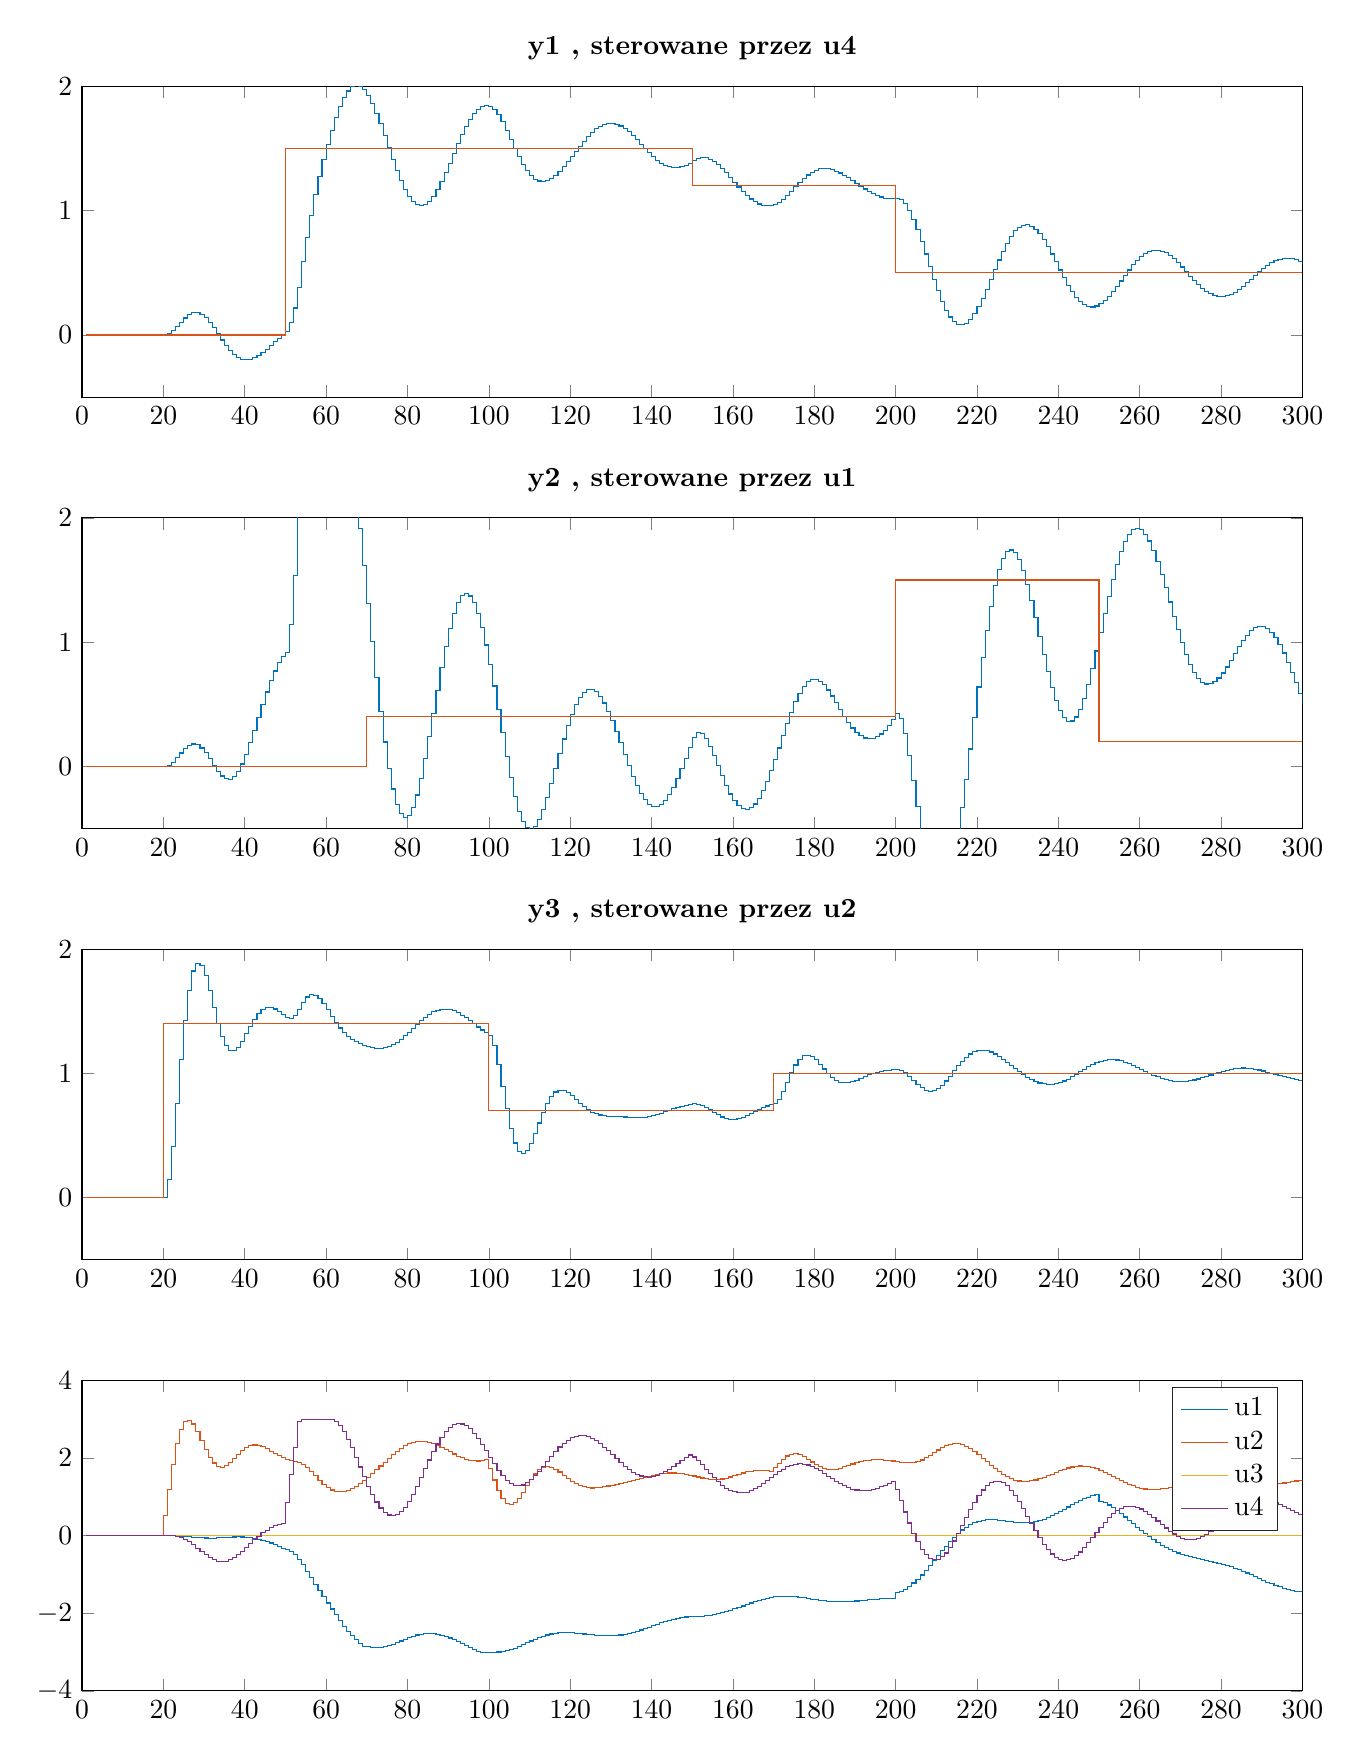
\begin{tikzpicture}

\begin{axis}[%
width=6.102in,
height=1.553in,
at={(1.024in,7.552in)},
scale only axis,
xmin=0,
xmax=300,
ymin=-0.5,
ymax=2,
axis background/.style={fill=white},
title style={font=\bfseries},
title={y1 , sterowane przez u4}
]
\addplot[const plot, color=mycolor1, forget plot] table[row sep=crcr] {%
1	0\\
2	0\\
3	0\\
4	0\\
5	0\\
6	0\\
7	0\\
8	0\\
9	0\\
10	0\\
11	0\\
12	0\\
13	0\\
14	0\\
15	0\\
16	0\\
17	0\\
18	0\\
19	0\\
20	0\\
21	0.0114581194369012\\
22	0.0352462992044872\\
23	0.0677297778748464\\
24	0.10352730709192\\
25	0.136975646202696\\
26	0.162975234664333\\
27	0.177644124618113\\
28	0.178700808914037\\
29	0.165576512770839\\
30	0.139293598730558\\
31	0.102168441520417\\
32	0.0574075471474105\\
33	0.00866540678464407\\
34	-0.0403762215561022\\
35	-0.0863623815918464\\
36	-0.126524275227483\\
37	-0.158832972969058\\
38	-0.182051481888024\\
39	-0.195700484745826\\
40	-0.199960069367418\\
41	-0.195532482307167\\
42	-0.183489926734973\\
43	-0.165127605405217\\
44	-0.141836678563861\\
45	-0.115005649620327\\
46	-0.0859528480931323\\
47	-0.0558878514844813\\
48	-0.0258962968592602\\
49	0.00305927708274754\\
50	0.0301302413219166\\
51	0.0982846132780422\\
52	0.217220328570168\\
53	0.383529281493918\\
54	0.58946937867999\\
55	0.784804947403667\\
56	0.964093730376323\\
57	1.12791971728541\\
58	1.27708027255889\\
59	1.41260043463201\\
60	1.53566311108234\\
61	1.64751342718795\\
62	1.7493676925246\\
63	1.83786869635353\\
64	1.91011486360851\\
65	1.96382113871435\\
66	1.99738641339324\\
67	2.00996192580095\\
68	2.00149248638164\\
69	1.97272488968493\\
70	1.92518061496398\\
71	1.86204341770004\\
72	1.78537630505093\\
73	1.69860482854744\\
74	1.60535591919893\\
75	1.50943269520064\\
76	1.41465550559872\\
77	1.32470446626275\\
78	1.24297314606529\\
79	1.17243934532522\\
80	1.11555797809217\\
81	1.0741796338108\\
82	1.04949693493388\\
83	1.04201942156368\\
84	1.0515764433509\\
85	1.07734646010247\\
86	1.11791026180309\\
87	1.1713249159624\\
88	1.23521472512273\\
89	1.30687511498266\\
90	1.38338515835075\\
91	1.46172435868622\\
92	1.53888935936453\\
93	1.61200640433004\\
94	1.67843564783836\\
95	1.73586379122257\\
96	1.78238200709252\\
97	1.81654668683346\\
98	1.83742120196003\\
99	1.8447730181463\\
100	1.83897841272924\\
101	1.81477870723029\\
102	1.77266297501403\\
103	1.71578769993969\\
104	1.64868119905615\\
105	1.57628879713651\\
106	1.50346367267524\\
107	1.43454758746727\\
108	1.37308516005184\\
109	1.32167555682358\\
110	1.28194686229913\\
111	1.25462722032482\\
112	1.23968117618045\\
113	1.23647923161599\\
114	1.24397238899826\\
115	1.26085001850253\\
116	1.28566727249598\\
117	1.31693616330572\\
118	1.35318126082632\\
119	1.39296605899347\\
120	1.43489908471492\\
121	1.47762980020635\\
122	1.51984356995714\\
123	1.56026289394341\\
124	1.59765929678662\\
125	1.63087724853027\\
126	1.65886874014944\\
127	1.68073498717429\\
128	1.69577038626928\\
129	1.70350335938537\\
130	1.70372902358927\\
131	1.69652956680524\\
132	1.6822795815997\\
133	1.66163518440274\\
134	1.63550731367703\\
135	1.60502098237306\\
136	1.57146333398744\\
137	1.53622405068366\\
138	1.50073197285652\\
139	1.46639174348291\\
140	1.43452395093038\\
141	1.40631169210534\\
142	1.38275580045004\\
143	1.3646402609515\\
144	1.35250863386401\\
145	1.34665167899613\\
146	1.34710584263578\\
147	1.3536618512279\\
148	1.36588234723784\\
149	1.38312729084253\\
150	1.40458571858739\\
151	1.42056968322882\\
152	1.4279701598947\\
153	1.42626595550014\\
154	1.41581285125935\\
155	1.39734877242894\\
156	1.3719392230408\\
157	1.34090304376721\\
158	1.30573119677258\\
159	1.26800639645813\\
160	1.22932807899738\\
161	1.19124574138388\\
162	1.15520230678378\\
163	1.12248805244081\\
164	1.09420484265986\\
165	1.07123994773005\\
166	1.05424855704343\\
167	1.04364413664877\\
168	1.03959594966466\\
169	1.04203326583163\\
170	1.05065596159518\\
171	1.06740661533284\\
172	1.09176947375362\\
173	1.1221015529261\\
174	1.15625751604959\\
175	1.19194110731142\\
176	1.22692706834301\\
177	1.25924367146072\\
178	1.28729728208898\\
179	1.30993738380658\\
180	1.32646822920431\\
181	1.33661803797513\\
182	1.34047910363488\\
183	1.33843240101719\\
184	1.33106875380792\\
185	1.31911590712164\\
186	1.30337756731637\\
187	1.28468717799432\\
188	1.263876339344\\
189	1.24175563952342\\
190	1.2191043860951\\
191	1.19666529412988\\
192	1.17514048431945\\
193	1.15518597415114\\
194	1.13740297942003\\
195	1.12232555703675\\
196	1.11040522063355\\
197	1.10199400676417\\
198	1.09732798051735\\
199	1.09651332335245\\
200	1.09951697209214\\
201	1.08837823739621\\
202	1.05579465469326\\
203	1.0028943545549\\
204	0.932371394014842\\
205	0.847627395284454\\
206	0.752596003663295\\
207	0.651527274738077\\
208	0.548768078442011\\
209	0.448555718013883\\
210	0.354835140383095\\
211	0.271106616218482\\
212	0.200307428243097\\
213	0.144728308649444\\
214	0.105963272870804\\
215	0.0848901308566349\\
216	0.0816782411577888\\
217	0.0958198642171212\\
218	0.126181595719355\\
219	0.17107264698811\\
220	0.228327042236181\\
221	0.295397019447849\\
222	0.369454999168948\\
223	0.447501416903164\\
224	0.526475532329495\\
225	0.603366090803565\\
226	0.67531849079777\\
227	0.739734975536924\\
228	0.794364376738173\\
229	0.837378132120929\\
230	0.867429691672282\\
231	0.883695012014245\\
232	0.88589258380487\\
233	0.87428229771633\\
234	0.849643373762849\\
235	0.813232496489474\\
236	0.766724156992257\\
237	0.712135951413269\\
238	0.651742184739147\\
239	0.587979551514842\\
240	0.523348897846631\\
241	0.460317110760336\\
242	0.401223041474421\\
243	0.348191067028286\\
244	0.303055454833803\\
245	0.267298145844951\\
246	0.242001944687236\\
247	0.22782042980511\\
248	0.22496520273724\\
249	0.233210410091481\\
250	0.251913818986082\\
251	0.276963245382422\\
252	0.309557915505599\\
253	0.347793737275535\\
254	0.390032113240999\\
255	0.434539049957177\\
256	0.479545771513266\\
257	0.523315261554297\\
258	0.564205158797248\\
259	0.600726100314469\\
260	0.631593466943631\\
261	0.655770663444104\\
262	0.672502361490502\\
263	0.681336513035587\\
264	0.682134391605637\\
265	0.675068414677767\\
266	0.660608012765202\\
267	0.639494310718524\\
268	0.612704846282127\\
269	0.581409946185144\\
270	0.546922692340896\\
271	0.510644627524029\\
272	0.474009464930978\\
273	0.438427079019899\\
274	0.405229970944227\\
275	0.375624230019469\\
276	0.350646765519751\\
277	0.331130275400561\\
278	0.317677066217655\\
279	0.310642457879337\\
280	0.310128113968633\\
281	0.315985248443533\\
282	0.327827286625527\\
283	0.345051215115573\\
284	0.366866552559967\\
285	0.392330620125326\\
286	0.420388594271753\\
287	0.449916690007209\\
288	0.479766753179522\\
289	0.508810536218674\\
290	0.535981991560015\\
291	0.560316037058207\\
292	0.580982422275817\\
293	0.597313545958945\\
294	0.608825334048816\\
295	0.615230573712867\\
296	0.616444400740259\\
297	0.612581943448626\\
298	0.603948424258271\\
299	0.591022299094685\\
300	0.574432264531452\\
};
\addplot[const plot, color=mycolor2, forget plot] table[row sep=crcr] {%
1	0\\
2	0\\
3	0\\
4	0\\
5	0\\
6	0\\
7	0\\
8	0\\
9	0\\
10	0\\
11	0\\
12	0\\
13	0\\
14	0\\
15	0\\
16	0\\
17	0\\
18	0\\
19	0\\
20	0\\
21	0\\
22	0\\
23	0\\
24	0\\
25	0\\
26	0\\
27	0\\
28	0\\
29	0\\
30	0\\
31	0\\
32	0\\
33	0\\
34	0\\
35	0\\
36	0\\
37	0\\
38	0\\
39	0\\
40	0\\
41	0\\
42	0\\
43	0\\
44	0\\
45	0\\
46	0\\
47	0\\
48	0\\
49	0\\
50	1.5\\
51	1.5\\
52	1.5\\
53	1.5\\
54	1.5\\
55	1.5\\
56	1.5\\
57	1.5\\
58	1.5\\
59	1.5\\
60	1.5\\
61	1.5\\
62	1.5\\
63	1.5\\
64	1.5\\
65	1.5\\
66	1.5\\
67	1.5\\
68	1.5\\
69	1.5\\
70	1.5\\
71	1.5\\
72	1.5\\
73	1.5\\
74	1.5\\
75	1.5\\
76	1.5\\
77	1.5\\
78	1.5\\
79	1.5\\
80	1.5\\
81	1.5\\
82	1.5\\
83	1.5\\
84	1.5\\
85	1.5\\
86	1.5\\
87	1.5\\
88	1.5\\
89	1.5\\
90	1.5\\
91	1.5\\
92	1.5\\
93	1.5\\
94	1.5\\
95	1.5\\
96	1.5\\
97	1.5\\
98	1.5\\
99	1.5\\
100	1.5\\
101	1.5\\
102	1.5\\
103	1.5\\
104	1.5\\
105	1.5\\
106	1.5\\
107	1.5\\
108	1.5\\
109	1.5\\
110	1.5\\
111	1.5\\
112	1.5\\
113	1.5\\
114	1.5\\
115	1.5\\
116	1.5\\
117	1.5\\
118	1.5\\
119	1.5\\
120	1.5\\
121	1.5\\
122	1.5\\
123	1.5\\
124	1.5\\
125	1.5\\
126	1.5\\
127	1.5\\
128	1.5\\
129	1.5\\
130	1.5\\
131	1.5\\
132	1.5\\
133	1.5\\
134	1.5\\
135	1.5\\
136	1.5\\
137	1.5\\
138	1.5\\
139	1.5\\
140	1.5\\
141	1.5\\
142	1.5\\
143	1.5\\
144	1.5\\
145	1.5\\
146	1.5\\
147	1.5\\
148	1.5\\
149	1.5\\
150	1.2\\
151	1.2\\
152	1.2\\
153	1.2\\
154	1.2\\
155	1.2\\
156	1.2\\
157	1.2\\
158	1.2\\
159	1.2\\
160	1.2\\
161	1.2\\
162	1.2\\
163	1.2\\
164	1.2\\
165	1.2\\
166	1.2\\
167	1.2\\
168	1.2\\
169	1.2\\
170	1.2\\
171	1.2\\
172	1.2\\
173	1.2\\
174	1.2\\
175	1.2\\
176	1.2\\
177	1.2\\
178	1.2\\
179	1.2\\
180	1.2\\
181	1.2\\
182	1.2\\
183	1.2\\
184	1.2\\
185	1.2\\
186	1.2\\
187	1.2\\
188	1.2\\
189	1.2\\
190	1.2\\
191	1.2\\
192	1.2\\
193	1.2\\
194	1.2\\
195	1.2\\
196	1.2\\
197	1.2\\
198	1.2\\
199	1.2\\
200	0.5\\
201	0.5\\
202	0.5\\
203	0.5\\
204	0.5\\
205	0.5\\
206	0.5\\
207	0.5\\
208	0.5\\
209	0.5\\
210	0.5\\
211	0.5\\
212	0.5\\
213	0.5\\
214	0.5\\
215	0.5\\
216	0.5\\
217	0.5\\
218	0.5\\
219	0.5\\
220	0.5\\
221	0.5\\
222	0.5\\
223	0.5\\
224	0.5\\
225	0.5\\
226	0.5\\
227	0.5\\
228	0.5\\
229	0.5\\
230	0.5\\
231	0.5\\
232	0.5\\
233	0.5\\
234	0.5\\
235	0.5\\
236	0.5\\
237	0.5\\
238	0.5\\
239	0.5\\
240	0.5\\
241	0.5\\
242	0.5\\
243	0.5\\
244	0.5\\
245	0.5\\
246	0.5\\
247	0.5\\
248	0.5\\
249	0.5\\
250	0.5\\
251	0.5\\
252	0.5\\
253	0.5\\
254	0.5\\
255	0.5\\
256	0.5\\
257	0.5\\
258	0.5\\
259	0.5\\
260	0.5\\
261	0.5\\
262	0.5\\
263	0.5\\
264	0.5\\
265	0.5\\
266	0.5\\
267	0.5\\
268	0.5\\
269	0.5\\
270	0.5\\
271	0.5\\
272	0.5\\
273	0.5\\
274	0.5\\
275	0.5\\
276	0.5\\
277	0.5\\
278	0.5\\
279	0.5\\
280	0.5\\
281	0.5\\
282	0.5\\
283	0.5\\
284	0.5\\
285	0.5\\
286	0.5\\
287	0.5\\
288	0.5\\
289	0.5\\
290	0.5\\
291	0.5\\
292	0.5\\
293	0.5\\
294	0.5\\
295	0.5\\
296	0.5\\
297	0.5\\
298	0.5\\
299	0.5\\
300	0.5\\
};
\end{axis}

\begin{axis}[%
width=6.102in,
height=1.553in,
at={(1.024in,5.395in)},
scale only axis,
xmin=0,
xmax=300,
ymin=-0.5,
ymax=2,
axis background/.style={fill=white},
title style={font=\bfseries},
title={y2 , sterowane przez u1}
]
\addplot[const plot, color=mycolor1, forget plot] table[row sep=crcr] {%
1	0\\
2	0\\
3	0\\
4	0\\
5	0\\
6	0\\
7	0\\
8	0\\
9	0\\
10	0\\
11	0\\
12	0\\
13	0\\
14	0\\
15	0\\
16	0\\
17	0\\
18	0\\
19	0\\
20	0\\
21	0.0105699306087332\\
22	0.0344208390223349\\
23	0.0688454456250659\\
24	0.107730184510059\\
25	0.143627215951997\\
26	0.169511023669733\\
27	0.180149350145648\\
28	0.172931058132085\\
29	0.148143595381919\\
30	0.108768274220769\\
31	0.0599095791909637\\
32	0.00799936887372107\\
33	-0.0400811112459731\\
34	-0.0778348655866105\\
35	-0.0998409844736308\\
36	-0.102242838314055\\
37	-0.0830071387704835\\
38	-0.0419607538955041\\
39	0.0193626866863902\\
40	0.0980181215863781\\
41	0.190030929836036\\
42	0.290810970056489\\
43	0.395551750554374\\
44	0.499579117850956\\
45	0.598627069707346\\
46	0.689031275480965\\
47	0.76784204632146\\
48	0.832866833067633\\
49	0.88265741304312\\
50	0.916458844294379\\
51	1.14159320783665\\
52	1.53851335233974\\
53	2.03784545785411\\
54	2.57679342187138\\
55	2.91371501739182\\
56	3.09994877071484\\
57	3.19146312143701\\
58	3.22233561812836\\
59	3.21356099715157\\
60	3.17829219421145\\
61	3.12495279208182\\
62	3.05908754464986\\
63	2.96324024829583\\
64	2.82876752445904\\
65	2.65320120240314\\
66	2.43831547413072\\
67	2.18890412304139\\
68	1.91191332662596\\
69	1.61577492694718\\
70	1.30985044959218\\
71	1.00676572936033\\
72	0.713917352956053\\
73	0.440855194035325\\
74	0.195897028757796\\
75	-0.0138006907272008\\
76	-0.182512266975804\\
77	-0.306153076696366\\
78	-0.382415319693918\\
79	-0.410826708564931\\
80	-0.392731260189034\\
81	-0.331195058943366\\
82	-0.230843322597989\\
83	-0.0976380536930493\\
84	0.0613921442269945\\
85	0.23845694051596\\
86	0.42532987180185\\
87	0.61368056236348\\
88	0.795399974342824\\
89	0.962906115433081\\
90	1.10941907500188\\
91	1.2291960175906\\
92	1.3177187378451\\
93	1.37182848608387\\
94	1.38980493283952\\
95	1.37138828768857\\
96	1.31774566431033\\
97	1.23138473759945\\
98	1.11601952156989\\
99	0.976916625658755\\
100	0.820390190735373\\
101	0.646796081294121\\
102	0.460696130895401\\
103	0.269444875724434\\
104	0.082402892155794\\
105	-0.0907649636267617\\
106	-0.241189269597469\\
107	-0.361677237062598\\
108	-0.447286511050729\\
109	-0.495582015252038\\
110	-0.506607234900645\\
111	-0.482626718906848\\
112	-0.427710508827115\\
113	-0.347233887487478\\
114	-0.247359253800476\\
115	-0.134553839948565\\
116	-0.0151804151660545\\
117	0.104819097454718\\
118	0.220142708506862\\
119	0.326258031224941\\
120	0.419458545868462\\
121	0.496866369336654\\
122	0.556401561760232\\
123	0.596735219765498\\
124	0.61723899421219\\
125	0.61793832240989\\
126	0.599471545257461\\
127	0.563052920432587\\
128	0.510434792244681\\
129	0.443862998271259\\
130	0.366019890823896\\
131	0.279950844018914\\
132	0.18897240312209\\
133	0.0965628672547797\\
134	0.00623865803070153\\
135	-0.0785780324437668\\
136	-0.154693342830099\\
137	-0.219269931296938\\
138	-0.269941698782237\\
139	-0.304908318549556\\
140	-0.323004232277418\\
141	-0.323738533734475\\
142	-0.307304092278628\\
143	-0.274556181781844\\
144	-0.226962619660169\\
145	-0.166528871395205\\
146	-0.0957026701311192\\
147	-0.0172634139749829\\
148	0.0657980525168495\\
149	0.150403652439503\\
150	0.233510926535709\\
151	0.270738289429375\\
152	0.263444100803785\\
153	0.223394186936702\\
154	0.161541543210045\\
155	0.0863788217915369\\
156	0.00489679944893623\\
157	-0.0769572165440149\\
158	-0.154084636739917\\
159	-0.222178014318445\\
160	-0.277727376705679\\
161	-0.318045905458611\\
162	-0.341289280387255\\
163	-0.346455387647113\\
164	-0.333359102906736\\
165	-0.302581862705018\\
166	-0.25539864480342\\
167	-0.193686445984998\\
168	-0.119818864122913\\
169	-0.0365513349994757\\
170	0.0530987763939061\\
171	0.148238463279004\\
172	0.246269411018997\\
173	0.343525407547773\\
174	0.435810243711868\\
175	0.518938199160421\\
176	0.589194246536445\\
177	0.643696680540553\\
178	0.680626467520761\\
179	0.699320153848369\\
180	0.700239864374844\\
181	0.684844833891555\\
182	0.655394914679106\\
183	0.614717710768122\\
184	0.565968248930171\\
185	0.512404580344186\\
186	0.457195692741603\\
187	0.403270798154859\\
188	0.353212426266759\\
189	0.309190479362933\\
190	0.272930849419697\\
191	0.245710415789351\\
192	0.228370042148521\\
193	0.221338213646382\\
194	0.224659753418819\\
195	0.238026177164963\\
196	0.260806284774834\\
197	0.292077245429386\\
198	0.330657521841835\\
199	0.375143434830511\\
200	0.423951030838694\\
201	0.386330077161481\\
202	0.263249067940997\\
203	0.0862597776202338\\
204	-0.117046506026437\\
205	-0.325822525795936\\
206	-0.523714003834448\\
207	-0.697753394901457\\
208	-0.837829756915647\\
209	-0.936450345611762\\
210	-0.988628616344909\\
211	-0.991800423697941\\
212	-0.945714219845096\\
213	-0.852269791892885\\
214	-0.715298559712382\\
215	-0.540289879487566\\
216	-0.334074294778919\\
217	-0.1044777526518\\
218	0.140038424114542\\
219	0.39073769666228\\
220	0.638955981461181\\
221	0.876426058777016\\
222	1.09556983960237\\
223	1.28975139029554\\
224	1.45348521101482\\
225	1.58259569287043\\
226	1.67432499710431\\
227	1.72738788089895\\
228	1.74197330407662\\
229	1.71969402981607\\
230	1.66348688771179\\
231	1.57746787075476\\
232	1.46674772997812\\
233	1.33721513060182\\
234	1.19529565027707\\
235	1.0476958440884\\
236	0.901142195845402\\
237	0.762124966018033\\
238	0.636656705768926\\
239	0.530054535701446\\
240	0.446754217518336\\
241	0.390162632149726\\
242	0.362553594037021\\
243	0.365010066204211\\
244	0.397413888806484\\
245	0.458482189079963\\
246	0.545847791238562\\
247	0.656179268798109\\
248	0.785334843560223\\
249	0.928543184307695\\
250	1.08060332745242\\
251	1.22690219556449\\
252	1.36975386644093\\
253	1.50324344767429\\
254	1.62317281057513\\
255	1.72590175431162\\
256	1.80845154742311\\
257	1.86860116567039\\
258	1.90494816256861\\
259	1.91693908536805\\
260	1.90486893135055\\
261	1.86985017631725\\
262	1.81375296617095\\
263	1.7391190559143\\
264	1.64905300414764\\
265	1.54709494847026\\
266	1.43707995743659\\
267	1.32298943967006\\
268	1.20880035961786\\
269	1.09833804266967\\
270	0.995138143819276\\
271	0.902322911685826\\
272	0.822496224899256\\
273	0.757661043521851\\
274	0.709161946176924\\
275	0.677654361572269\\
276	0.663101001455387\\
277	0.664794910626007\\
278	0.681407515297224\\
279	0.71105911546235\\
280	0.751408464823899\\
281	0.799757440315436\\
282	0.853166341063913\\
283	0.90857508425414\\
284	0.962925485221744\\
285	1.01327991624137\\
286	1.05693192124444\\
287	1.0915048046464\\
288	1.11503478928443\\
289	1.12603602500042\\
290	1.12354549664596\\
291	1.10714669742881\\
292	1.07697176899945\\
293	1.03368263221345\\
294	0.978432412137122\\
295	0.912809169921148\\
296	0.838764568196173\\
297	0.758530595215249\\
298	0.67452784035569\\
299	0.589269039284537\\
300	0.505261686107263\\
};
\addplot[const plot, color=mycolor2, forget plot] table[row sep=crcr] {%
1	0\\
2	0\\
3	0\\
4	0\\
5	0\\
6	0\\
7	0\\
8	0\\
9	0\\
10	0\\
11	0\\
12	0\\
13	0\\
14	0\\
15	0\\
16	0\\
17	0\\
18	0\\
19	0\\
20	0\\
21	0\\
22	0\\
23	0\\
24	0\\
25	0\\
26	0\\
27	0\\
28	0\\
29	0\\
30	0\\
31	0\\
32	0\\
33	0\\
34	0\\
35	0\\
36	0\\
37	0\\
38	0\\
39	0\\
40	0\\
41	0\\
42	0\\
43	0\\
44	0\\
45	0\\
46	0\\
47	0\\
48	0\\
49	0\\
50	0\\
51	0\\
52	0\\
53	0\\
54	0\\
55	0\\
56	0\\
57	0\\
58	0\\
59	0\\
60	0\\
61	0\\
62	0\\
63	0\\
64	0\\
65	0\\
66	0\\
67	0\\
68	0\\
69	0\\
70	0.4\\
71	0.4\\
72	0.4\\
73	0.4\\
74	0.4\\
75	0.4\\
76	0.4\\
77	0.4\\
78	0.4\\
79	0.4\\
80	0.4\\
81	0.4\\
82	0.4\\
83	0.4\\
84	0.4\\
85	0.4\\
86	0.4\\
87	0.4\\
88	0.4\\
89	0.4\\
90	0.4\\
91	0.4\\
92	0.4\\
93	0.4\\
94	0.4\\
95	0.4\\
96	0.4\\
97	0.4\\
98	0.4\\
99	0.4\\
100	0.4\\
101	0.4\\
102	0.4\\
103	0.4\\
104	0.4\\
105	0.4\\
106	0.4\\
107	0.4\\
108	0.4\\
109	0.4\\
110	0.4\\
111	0.4\\
112	0.4\\
113	0.4\\
114	0.4\\
115	0.4\\
116	0.4\\
117	0.4\\
118	0.4\\
119	0.4\\
120	0.4\\
121	0.4\\
122	0.4\\
123	0.4\\
124	0.4\\
125	0.4\\
126	0.4\\
127	0.4\\
128	0.4\\
129	0.4\\
130	0.4\\
131	0.4\\
132	0.4\\
133	0.4\\
134	0.4\\
135	0.4\\
136	0.4\\
137	0.4\\
138	0.4\\
139	0.4\\
140	0.4\\
141	0.4\\
142	0.4\\
143	0.4\\
144	0.4\\
145	0.4\\
146	0.4\\
147	0.4\\
148	0.4\\
149	0.4\\
150	0.4\\
151	0.4\\
152	0.4\\
153	0.4\\
154	0.4\\
155	0.4\\
156	0.4\\
157	0.4\\
158	0.4\\
159	0.4\\
160	0.4\\
161	0.4\\
162	0.4\\
163	0.4\\
164	0.4\\
165	0.4\\
166	0.4\\
167	0.4\\
168	0.4\\
169	0.4\\
170	0.4\\
171	0.4\\
172	0.4\\
173	0.4\\
174	0.4\\
175	0.4\\
176	0.4\\
177	0.4\\
178	0.4\\
179	0.4\\
180	0.4\\
181	0.4\\
182	0.4\\
183	0.4\\
184	0.4\\
185	0.4\\
186	0.4\\
187	0.4\\
188	0.4\\
189	0.4\\
190	0.4\\
191	0.4\\
192	0.4\\
193	0.4\\
194	0.4\\
195	0.4\\
196	0.4\\
197	0.4\\
198	0.4\\
199	0.4\\
200	1.5\\
201	1.5\\
202	1.5\\
203	1.5\\
204	1.5\\
205	1.5\\
206	1.5\\
207	1.5\\
208	1.5\\
209	1.5\\
210	1.5\\
211	1.5\\
212	1.5\\
213	1.5\\
214	1.5\\
215	1.5\\
216	1.5\\
217	1.5\\
218	1.5\\
219	1.5\\
220	1.5\\
221	1.5\\
222	1.5\\
223	1.5\\
224	1.5\\
225	1.5\\
226	1.5\\
227	1.5\\
228	1.5\\
229	1.5\\
230	1.5\\
231	1.5\\
232	1.5\\
233	1.5\\
234	1.5\\
235	1.5\\
236	1.5\\
237	1.5\\
238	1.5\\
239	1.5\\
240	1.5\\
241	1.5\\
242	1.5\\
243	1.5\\
244	1.5\\
245	1.5\\
246	1.5\\
247	1.5\\
248	1.5\\
249	1.5\\
250	0.2\\
251	0.2\\
252	0.2\\
253	0.2\\
254	0.2\\
255	0.2\\
256	0.2\\
257	0.2\\
258	0.2\\
259	0.2\\
260	0.2\\
261	0.2\\
262	0.2\\
263	0.2\\
264	0.2\\
265	0.2\\
266	0.2\\
267	0.2\\
268	0.2\\
269	0.2\\
270	0.2\\
271	0.2\\
272	0.2\\
273	0.2\\
274	0.2\\
275	0.2\\
276	0.2\\
277	0.2\\
278	0.2\\
279	0.2\\
280	0.2\\
281	0.2\\
282	0.2\\
283	0.2\\
284	0.2\\
285	0.2\\
286	0.2\\
287	0.2\\
288	0.2\\
289	0.2\\
290	0.2\\
291	0.2\\
292	0.2\\
293	0.2\\
294	0.2\\
295	0.2\\
296	0.2\\
297	0.2\\
298	0.2\\
299	0.2\\
300	0.2\\
};
\end{axis}

\begin{axis}[%
width=6.102in,
height=1.553in,
at={(1.024in,3.239in)},
scale only axis,
xmin=0,
xmax=300,
ymin=-0.5,
ymax=2,
axis background/.style={fill=white},
title style={font=\bfseries},
title={y3 , sterowane przez u2}
]
\addplot[const plot, color=mycolor1, forget plot] table[row sep=crcr] {%
1	0\\
2	0\\
3	0\\
4	0\\
5	0\\
6	0\\
7	0\\
8	0\\
9	0\\
10	0\\
11	0\\
12	0\\
13	0\\
14	0\\
15	0\\
16	0\\
17	0\\
18	0\\
19	0\\
20	0\\
21	0.142671982788199\\
22	0.414294892302412\\
23	0.757125589391064\\
24	1.11069063710109\\
25	1.42608079115622\\
26	1.66945325239224\\
27	1.82334504259659\\
28	1.88561956526174\\
29	1.86663870669794\\
30	1.78538959174395\\
31	1.66527730645761\\
32	1.53019375842929\\
33	1.40131369825414\\
34	1.29488399654906\\
35	1.22109061267357\\
36	1.18393200360796\\
37	1.18191275655349\\
38	1.20930350624936\\
39	1.25769183735851\\
40	1.31756720929934\\
41	1.37973055942624\\
42	1.43638407436178\\
43	1.48182683976819\\
44	1.51274756784709\\
45	1.52815890601044\\
46	1.52905457814298\\
47	1.51788944837836\\
48	1.49798475174277\\
49	1.47294932862093\\
50	1.44618696244409\\
51	1.44183508390726\\
52	1.46501338675926\\
53	1.51126278988571\\
54	1.5714225972266\\
55	1.61452886648856\\
56	1.63384720767233\\
57	1.62895585654501\\
58	1.60289895719273\\
59	1.56119105560387\\
60	1.51053430569624\\
61	1.45765225358583\\
62	1.40837454491055\\
63	1.36485770957768\\
64	1.3279873896602\\
65	1.2976447830702\\
66	1.2730700229624\\
67	1.25323659757602\\
68	1.23716303702171\\
69	1.22413186100842\\
70	1.21380380632125\\
71	1.2067882868882\\
72	1.20300703256069\\
73	1.20303854521913\\
74	1.20742511938894\\
75	1.21661108236533\\
76	1.23082418720919\\
77	1.24999082186349\\
78	1.27369507987838\\
79	1.30118212857246\\
80	1.33140132472831\\
81	1.3630802948327\\
82	1.3948187843948\\
83	1.42519043472778\\
84	1.45284150416757\\
85	1.47657752217418\\
86	1.49543149753742\\
87	1.50871015399168\\
88	1.51601735919976\\
89	1.5172561654065\\
90	1.51261252404261\\
91	1.5025247144638\\
92	1.48764287538254\\
93	1.4687828523928\\
94	1.44687802325894\\
95	1.42293199446368\\
96	1.39797422756763\\
97	1.37301987422214\\
98	1.34903445855277\\
99	1.32700620810771\\
100	1.3078647917449\\
101	1.22082539751576\\
102	1.07312444618372\\
103	0.893845728436913\\
104	0.713376265417996\\
105	0.556188288970315\\
106	0.439091300533846\\
107	0.370577185568541\\
108	0.351351099064014\\
109	0.375753763424198\\
110	0.433711382137052\\
111	0.512857755117594\\
112	0.600523154917692\\
113	0.685363543594122\\
114	0.758495734500143\\
115	0.814094646225216\\
116	0.849486524803266\\
117	0.864829544100402\\
118	0.86250725064163\\
119	0.84637130371295\\
120	0.820961166101688\\
121	0.79080499267608\\
122	0.759873939665348\\
123	0.731227362076268\\
124	0.706853918742949\\
125	0.687687179337609\\
126	0.673756107731442\\
127	0.664421461405874\\
128	0.658648092424272\\
129	0.655268811162797\\
130	0.653205774976049\\
131	0.65162801536423\\
132	0.650036601613974\\
133	0.648280337373117\\
134	0.646513619547496\\
135	0.645113558770889\\
136	0.644575611371634\\
137	0.645406187329442\\
138	0.64802766151105\\
139	0.652706763286013\\
140	0.65951230345654\\
141	0.668303370407038\\
142	0.678745067894969\\
143	0.690345939807067\\
144	0.702509580190532\\
145	0.7145925154739\\
146	0.725961077935185\\
147	0.736041379863418\\
148	0.744358323271258\\
149	0.750561528177153\\
150	0.754437869565913\\
151	0.751651655291032\\
152	0.741642651622435\\
153	0.725707730947481\\
154	0.706015002452459\\
155	0.685048463133335\\
156	0.665247208999563\\
157	0.648702737049734\\
158	0.636951774517564\\
159	0.630873334063002\\
160	0.630682659367253\\
161	0.636004224595521\\
162	0.645999689255122\\
163	0.659524754267621\\
164	0.675290591680437\\
165	0.69200995431206\\
166	0.708514091524768\\
167	0.72383310845751\\
168	0.737238475425622\\
169	0.748251337539742\\
170	0.756623693583063\\
171	0.792873855935696\\
172	0.854154786790147\\
173	0.928286197611338\\
174	1.00256058158247\\
175	1.06677331089367\\
176	1.11395103313751\\
177	1.14062164967145\\
178	1.14658592423819\\
179	1.13431489939325\\
180	1.10812626849783\\
181	1.07328922416275\\
182	1.0351862119907\\
183	0.998626733894411\\
184	0.967369616064766\\
185	0.943872071047232\\
186	0.929251201775763\\
187	0.923419415712278\\
188	0.925340913941375\\
189	0.933351817749018\\
190	0.945490206250733\\
191	0.95979218830034\\
192	0.974523598361552\\
193	0.988331515554872\\
194	1.00031344085414\\
195	1.01001306945457\\
196	1.01735924830814\\
197	1.02256862882052\\
198	1.02603296749617\\
199	1.028209645705\\
200	1.02952965873715\\
201	1.02192106661982\\
202	1.00291122468659\\
203	0.975222048397098\\
204	0.943047959660703\\
205	0.911095266664261\\
206	0.883864670097945\\
207	0.865052807193355\\
208	0.857156636747724\\
209	0.861294365207246\\
210	0.877225546730473\\
211	0.90353168937111\\
212	0.937906227859662\\
213	0.977499171838603\\
214	1.01926575299356\\
215	1.06027792808762\\
216	1.09797031494486\\
217	1.13030578215773\\
218	1.15585856373806\\
219	1.17382303123356\\
220	1.18396332574539\\
221	1.1865227035227\\
222	1.18211194017167\\
223	1.1715940815544\\
224	1.15597903691766\\
225	1.13633684910227\\
226	1.11373374628302\\
227	1.08919091958813\\
228	1.06366281204588\\
229	1.03802975514008\\
230	1.01309905429318\\
231	0.989608945298125\\
232	0.968230952462111\\
233	0.949567756497653\\
234	0.934145407023086\\
235	0.922400314325887\\
236	0.914662721570642\\
237	0.911139169342287\\
238	0.911896780261059\\
239	0.916852045963385\\
240	0.925766280110329\\
241	0.938249130344232\\
242	0.953770651790878\\
243	0.971681559972698\\
244	0.991240505473121\\
245	1.01164661969517\\
246	1.03207521036775\\
247	1.05171434484697\\
248	1.06980012968211\\
249	1.08564873789787\\
250	1.09868360137761\\
251	1.10664920216614\\
252	1.11072343734551\\
253	1.11075228215402\\
254	1.10700987521659\\
255	1.09990058058373\\
256	1.0899137921348\\
257	1.07758932974476\\
258	1.06348850919584\\
259	1.04817339325269\\
260	1.03219294239311\\
261	1.016074158399\\
262	1.00031611107203\\
263	0.985384918545007\\
264	0.971708222170963\\
265	0.959668327422386\\
266	0.949593846775058\\
267	0.941750272809252\\
268	0.936330353070386\\
269	0.933445390079376\\
270	0.93311864106052\\
271	0.935281861570322\\
272	0.939775765036506\\
273	0.94635480786855\\
274	0.954696312110302\\
275	0.964413555235592\\
276	0.975072130688808\\
277	0.986208641369243\\
278	0.997350645833557\\
279	1.00803673495118\\
280	1.01783566578161\\
281	1.02636360261241\\
282	1.03329869120512\\
283	1.03839239906085\\
284	1.04147727119208\\
285	1.04247096013659\\
286	1.04137657789357\\
287	1.03827957795107\\
288	1.03334150383449\\
289	1.02679103643803\\
290	1.018912838144\\
291	1.01003473119097\\
292	1.00051376521516\\
293	0.990721728401093\\
294	0.98103064154792\\
295	0.971798746963535\\
296	0.963357465924891\\
297	0.955999750298276\\
298	0.94997019625257\\
299	0.94545722127144\\
300	0.94258753063552\\
};
\addplot[const plot, color=mycolor2, forget plot] table[row sep=crcr] {%
1	0\\
2	0\\
3	0\\
4	0\\
5	0\\
6	0\\
7	0\\
8	0\\
9	0\\
10	0\\
11	0\\
12	0\\
13	0\\
14	0\\
15	0\\
16	0\\
17	0\\
18	0\\
19	0\\
20	1.4\\
21	1.4\\
22	1.4\\
23	1.4\\
24	1.4\\
25	1.4\\
26	1.4\\
27	1.4\\
28	1.4\\
29	1.4\\
30	1.4\\
31	1.4\\
32	1.4\\
33	1.4\\
34	1.4\\
35	1.4\\
36	1.4\\
37	1.4\\
38	1.4\\
39	1.4\\
40	1.4\\
41	1.4\\
42	1.4\\
43	1.4\\
44	1.4\\
45	1.4\\
46	1.4\\
47	1.4\\
48	1.4\\
49	1.4\\
50	1.4\\
51	1.4\\
52	1.4\\
53	1.4\\
54	1.4\\
55	1.4\\
56	1.4\\
57	1.4\\
58	1.4\\
59	1.4\\
60	1.4\\
61	1.4\\
62	1.4\\
63	1.4\\
64	1.4\\
65	1.4\\
66	1.4\\
67	1.4\\
68	1.4\\
69	1.4\\
70	1.4\\
71	1.4\\
72	1.4\\
73	1.4\\
74	1.4\\
75	1.4\\
76	1.4\\
77	1.4\\
78	1.4\\
79	1.4\\
80	1.4\\
81	1.4\\
82	1.4\\
83	1.4\\
84	1.4\\
85	1.4\\
86	1.4\\
87	1.4\\
88	1.4\\
89	1.4\\
90	1.4\\
91	1.4\\
92	1.4\\
93	1.4\\
94	1.4\\
95	1.4\\
96	1.4\\
97	1.4\\
98	1.4\\
99	1.4\\
100	0.7\\
101	0.7\\
102	0.7\\
103	0.7\\
104	0.7\\
105	0.7\\
106	0.7\\
107	0.7\\
108	0.7\\
109	0.7\\
110	0.7\\
111	0.7\\
112	0.7\\
113	0.7\\
114	0.7\\
115	0.7\\
116	0.7\\
117	0.7\\
118	0.7\\
119	0.7\\
120	0.7\\
121	0.7\\
122	0.7\\
123	0.7\\
124	0.7\\
125	0.7\\
126	0.7\\
127	0.7\\
128	0.7\\
129	0.7\\
130	0.7\\
131	0.7\\
132	0.7\\
133	0.7\\
134	0.7\\
135	0.7\\
136	0.7\\
137	0.7\\
138	0.7\\
139	0.7\\
140	0.7\\
141	0.7\\
142	0.7\\
143	0.7\\
144	0.7\\
145	0.7\\
146	0.7\\
147	0.7\\
148	0.7\\
149	0.7\\
150	0.7\\
151	0.7\\
152	0.7\\
153	0.7\\
154	0.7\\
155	0.7\\
156	0.7\\
157	0.7\\
158	0.7\\
159	0.7\\
160	0.7\\
161	0.7\\
162	0.7\\
163	0.7\\
164	0.7\\
165	0.7\\
166	0.7\\
167	0.7\\
168	0.7\\
169	0.7\\
170	1\\
171	1\\
172	1\\
173	1\\
174	1\\
175	1\\
176	1\\
177	1\\
178	1\\
179	1\\
180	1\\
181	1\\
182	1\\
183	1\\
184	1\\
185	1\\
186	1\\
187	1\\
188	1\\
189	1\\
190	1\\
191	1\\
192	1\\
193	1\\
194	1\\
195	1\\
196	1\\
197	1\\
198	1\\
199	1\\
200	1\\
201	1\\
202	1\\
203	1\\
204	1\\
205	1\\
206	1\\
207	1\\
208	1\\
209	1\\
210	1\\
211	1\\
212	1\\
213	1\\
214	1\\
215	1\\
216	1\\
217	1\\
218	1\\
219	1\\
220	1\\
221	1\\
222	1\\
223	1\\
224	1\\
225	1\\
226	1\\
227	1\\
228	1\\
229	1\\
230	1\\
231	1\\
232	1\\
233	1\\
234	1\\
235	1\\
236	1\\
237	1\\
238	1\\
239	1\\
240	1\\
241	1\\
242	1\\
243	1\\
244	1\\
245	1\\
246	1\\
247	1\\
248	1\\
249	1\\
250	1\\
251	1\\
252	1\\
253	1\\
254	1\\
255	1\\
256	1\\
257	1\\
258	1\\
259	1\\
260	1\\
261	1\\
262	1\\
263	1\\
264	1\\
265	1\\
266	1\\
267	1\\
268	1\\
269	1\\
270	1\\
271	1\\
272	1\\
273	1\\
274	1\\
275	1\\
276	1\\
277	1\\
278	1\\
279	1\\
280	1\\
281	1\\
282	1\\
283	1\\
284	1\\
285	1\\
286	1\\
287	1\\
288	1\\
289	1\\
290	1\\
291	1\\
292	1\\
293	1\\
294	1\\
295	1\\
296	1\\
297	1\\
298	1\\
299	1\\
300	1\\
};
\end{axis}

\begin{axis}[%
width=6.102in,
height=1.553in,
at={(1.024in,1.083in)},
scale only axis,
xmin=0,
xmax=300,
ymin=-4,
ymax=4,
axis background/.style={fill=white},
legend style={legend cell align=left, align=left, draw=white!15!black}
]
\addplot[const plot, color=mycolor1] table[row sep=crcr] {%
1	0\\
2	0\\
3	0\\
4	0\\
5	0\\
6	0\\
7	0\\
8	0\\
9	0\\
10	0\\
11	0\\
12	0\\
13	0\\
14	0\\
15	0\\
16	0\\
17	0\\
18	0\\
19	0\\
20	0\\
21	0\\
22	-0.00153263993826632\\
23	-0.00530811957650055\\
24	-0.0115437113167413\\
25	-0.0199357786042639\\
26	-0.029749662611148\\
27	-0.0399662348989809\\
28	-0.0494666672671205\\
29	-0.0572147159029179\\
30	-0.0624114525510194\\
31	-0.0646049600067519\\
32	-0.0637463693616916\\
33	-0.0601920417258357\\
34	-0.054658544758511\\
35	-0.0481418044192138\\
36	-0.041814248988078\\
37	-0.0369140533352753\\
38	-0.034639124930199\\
39	-0.0360557798076754\\
40	-0.0420287132997753\\
41	-0.0531754168829551\\
42	-0.0698450714604747\\
43	-0.0921194676192491\\
44	-0.119831828489858\\
45	-0.152598568665623\\
46	-0.189858930231416\\
47	-0.23091793451683\\
48	-0.274988975947278\\
49	-0.321233456924736\\
50	-0.36879593693964\\
51	-0.416834203523719\\
52	-0.494625599827042\\
53	-0.604755993900977\\
54	-0.746146413927485\\
55	-0.916199499492409\\
56	-1.0831138426561\\
57	-1.24906505584712\\
58	-1.41360740017111\\
59	-1.57582678124877\\
60	-1.73505379217972\\
61	-1.89079335803052\\
62	-2.0426791304911\\
63	-2.19044309726015\\
64	-2.33081692146994\\
65	-2.46139733485548\\
66	-2.58006804885706\\
67	-2.68508100481884\\
68	-2.77512984718287\\
69	-2.84939961487649\\
70	-2.84959502918267\\
71	-2.87994749430713\\
72	-2.88761122190022\\
73	-2.88154818819426\\
74	-2.86350701032664\\
75	-2.83549207924158\\
76	-2.79977992465969\\
77	-2.75882066595699\\
78	-2.71514136672369\\
79	-2.67124850384863\\
80	-2.62953333133759\\
81	-2.59218406370127\\
82	-2.56110834090492\\
83	-2.53786886570292\\
84	-2.52363442883733\\
85	-2.51914779947298\\
86	-2.52471119818783\\
87	-2.54018932432431\\
88	-2.56502920942012\\
89	-2.59829553846406\\
90	-2.6387195393997\\
91	-2.68475910148703\\
92	-2.73466745272111\\
93	-2.78656750918577\\
94	-2.83852890516756\\
95	-2.88864471928654\\
96	-2.93510502344652\\
97	-2.97626459034412\\
98	-3\\
99	-3\\
100	-3\\
101	-3\\
102	-2.99897889236625\\
103	-2.98780608581197\\
104	-2.96683145936493\\
105	-2.93700764063711\\
106	-2.89975928582781\\
107	-2.85687287039637\\
108	-2.81035113775346\\
109	-2.76226369052136\\
110	-2.71460870233939\\
111	-2.66919685481177\\
112	-2.62756417227881\\
113	-2.59091607647515\\
114	-2.56010133692645\\
115	-2.5356119320099\\
116	-2.51760326165466\\
117	-2.50592860797366\\
118	-2.50018204804972\\
119	-2.4997449362726\\
120	-2.50383232127102\\
121	-2.51153699100122\\
122	-2.52187004240466\\
123	-2.53379780730355\\
124	-2.54627556195385\\
125	-2.55827869707679\\
126	-2.56883197388713\\
127	-2.57703722075657\\
128	-2.58209943296289\\
129	-2.58335082289377\\
130	-2.58027201494361\\
131	-2.57250935015678\\
132	-2.5598871950602\\
133	-2.5424142442672\\
134	-2.52028305054048\\
135	-2.49386237428308\\
136	-2.46368237125029\\
137	-2.43041308343158\\
138	-2.39483711717011\\
139	-2.35781774608923\\
140	-2.32026393663356\\
141	-2.28309394561089\\
142	-2.2471991785603\\
143	-2.21340993191382\\
144	-2.1824644854928\\
145	-2.15498278470142\\
146	-2.1314456759744\\
147	-2.11218035662263\\
148	-2.09735239123343\\
149	-2.08696434805288\\
150	-2.08086083333767\\
151	-2.07873945870514\\
152	-2.07415082716958\\
153	-2.06588553703247\\
154	-2.05339638833444\\
155	-2.03639846261825\\
156	-2.0148139980476\\
157	-1.98882130032587\\
158	-1.95882694842619\\
159	-1.92543269199045\\
160	-1.88939746880848\\
161	-1.85159577809798\\
162	-1.81297420984127\\
163	-1.77450799577874\\
164	-1.73715931370527\\
165	-1.70183882775547\\
166	-1.66937164674457\\
167	-1.64046857540102\\
168	-1.61570324763149\\
169	-1.59549548072587\\
170	-1.58010097760538\\
171	-1.56960732642498\\
172	-1.56426451761515\\
173	-1.5639881344637\\
174	-1.56844310555652\\
175	-1.57705555724713\\
176	-1.58905392624948\\
177	-1.60352540396805\\
178	-1.61948284827795\\
179	-1.63593245273702\\
180	-1.65193576489096\\
181	-1.66666125688317\\
182	-1.6794225764713\\
183	-1.68970248048974\\
184	-1.69716303004085\\
185	-1.70164378769097\\
186	-1.70315045742927\\
187	-1.70183667111583\\
188	-1.69798152378988\\
189	-1.69196509766559\\
190	-1.68424370411563\\
191	-1.67532602068008\\
192	-1.66575079287353\\
193	-1.65606636815769\\
194	-1.64681206260512\\
195	-1.63850123312449\\
196	-1.63160592144317\\
197	-1.62654301742993\\
198	-1.62366201881138\\
199	-1.62323460194956\\
200	-1.46594632989676\\
201	-1.4378908847997\\
202	-1.37765724613828\\
203	-1.30487942273293\\
204	-1.21984004921787\\
205	-1.12321341277653\\
206	-1.01615469028157\\
207	-0.900344820071578\\
208	-0.777881237735909\\
209	-0.651163283320119\\
210	-0.522773337353684\\
211	-0.395357382590712\\
212	-0.271509605121939\\
213	-0.153665519642766\\
214	-0.0440075266265244\\
215	0.0556140228609911\\
216	0.143742116857622\\
217	0.219355524653743\\
218	0.281892052478429\\
219	0.331253025322442\\
220	0.36779003313262\\
221	0.39227548245462\\
222	0.405858887866743\\
223	0.410011138254533\\
224	0.406459197040412\\
225	0.397113854535202\\
226	0.383993250529784\\
227	0.369144926409462\\
228	0.3545691444887\\
229	0.342146121758885\\
230	0.333569659786386\\
231	0.330289408415492\\
232	0.333463678646586\\
233	0.343924325182321\\
234	0.362154762777446\\
235	0.388281678906918\\
236	0.422080478683927\\
237	0.462993969350968\\
238	0.510163284918806\\
239	0.562469589757478\\
240	0.618584703923834\\
241	0.677028479873963\\
242	0.736230542512832\\
243	0.794593889724316\\
244	0.850557840795968\\
245	0.902657912651772\\
246	0.949580391123839\\
247	0.990209635362313\\
248	1.02366649359742\\
249	1.0493366013682\\
250	0.87838776127705\\
251	0.848776048120629\\
252	0.786573748734653\\
253	0.717441124041585\\
254	0.64245447485823\\
255	0.562572336478562\\
256	0.478916586366031\\
257	0.392706357524013\\
258	0.305213081369232\\
259	0.217715700900417\\
260	0.131456548904032\\
261	0.0475995854241558\\
262	-0.0328075447438938\\
263	-0.108866333189208\\
264	-0.179854008713467\\
265	-0.24524306220815\\
266	-0.304713115377645\\
267	-0.358154850214823\\
268	-0.40566602283118\\
269	-0.447539888562444\\
270	-0.484246652186893\\
271	-0.516408815326033\\
272	-0.544771511834655\\
273	-0.570169092477562\\
274	-0.593489336158533\\
275	-0.615636722847159\\
276	-0.637496202335229\\
277	-0.659898834888987\\
278	-0.683590568993834\\
279	-0.709205264019049\\
280	-0.737242869714429\\
281	-0.768053449141669\\
282	-0.801827486841905\\
283	-0.838592669956375\\
284	-0.878217076757185\\
285	-0.92041846424639\\
286	-0.96477912298597\\
287	-1.01076557090309\\
288	-1.05775219495854\\
289	-1.10504782529533\\
290	-1.15192414424561\\
291	-1.19764479416991\\
292	-1.24149405368282\\
293	-1.28280399991634\\
294	-1.32097916210093\\
295	-1.35551779453626\\
296	-1.38602904942332\\
297	-1.41224550551358\\
298	-1.43403069987565\\
299	-1.4513815096414\\
300	-1.46442543060106\\
};
\addlegendentry{u1}

\addplot[const plot, color=mycolor2] table[row sep=crcr] {%
1	0\\
2	0\\
3	0\\
4	0\\
5	0\\
6	0\\
7	0\\
8	0\\
9	0\\
10	0\\
11	0\\
12	0\\
13	0\\
14	0\\
15	0\\
16	0\\
17	0\\
18	0\\
19	0\\
20	0.518\\
21	1.19\\
22	1.83721136636837\\
23	2.36822833810977\\
24	2.73966599222605\\
25	2.93714074381958\\
26	2.97217236922284\\
27	2.8753919660685\\
28	2.68859282672149\\
29	2.45695656784118\\
30	2.22241519333222\\
31	2.01877839534495\\
32	1.86890016272984\\
33	1.78384017656579\\
34	1.76372724865538\\
35	1.79987178795569\\
36	1.87760474768099\\
37	1.97933225902097\\
38	2.08737020644583\\
39	2.18623886584052\\
40	2.26423124519938\\
41	2.3141992055242\\
42	2.33361266876639\\
43	2.32402885552966\\
44	2.2901560654471\\
45	2.23871083148194\\
46	2.17725326699954\\
47	2.11315064206854\\
48	2.05277236445261\\
49	2.00096907542331\\
50	1.96084171217429\\
51	1.93376841488682\\
52	1.91174988139987\\
53	1.88216932982026\\
54	1.83301392334088\\
55	1.75604838774443\\
56	1.65559096565102\\
57	1.54204087155399\\
58	1.42731343445861\\
59	1.3223787319239\\
60	1.23584003892836\\
61	1.17315335056048\\
62	1.13643942199505\\
63	1.12478840636978\\
64	1.13571680881417\\
65	1.16605963568814\\
66	1.21255529889799\\
67	1.27221871647097\\
68	1.34253057718058\\
69	1.42146282728993\\
70	1.50738137269291\\
71	1.59887619890269\\
72	1.69436347683855\\
73	1.79222808710697\\
74	1.89063728605645\\
75	1.98749561125722\\
76	2.08047197674488\\
77	2.16709130602952\\
78	2.24487181969971\\
79	2.31148916599554\\
80	2.36494550319984\\
81	2.40372307730982\\
82	2.42690557993016\\
83	2.43425577077792\\
84	2.42624363774856\\
85	2.40402495769861\\
86	2.36937490034118\\
87	2.32458488872982\\
88	2.2723331165803\\
89	2.21553994678655\\
90	2.15721905299434\\
91	2.10033389371986\\
92	2.04766724841544\\
93	2.00170941545203\\
94	1.96456854948534\\
95	1.93790470960867\\
96	1.92288763205077\\
97	1.92017708799457\\
98	1.92992392961066\\
99	1.95178950923035\\
100	1.72594302430524\\
101	1.43308167929673\\
102	1.1609710309618\\
103	0.953466896312195\\
104	0.830283779760013\\
105	0.79654904250362\\
106	0.844411071819886\\
107	0.956499053527268\\
108	1.10996168602878\\
109	1.28041646295188\\
110	1.44532740587651\\
111	1.58649425852786\\
112	1.69151356183079\\
113	1.75423141380557\\
114	1.77433220053244\\
115	1.75628832587368\\
116	1.70793150510346\\
117	1.63890116515147\\
118	1.55918882318146\\
119	1.47794016009695\\
120	1.40261038927057\\
121	1.33850376939169\\
122	1.28867276775609\\
123	1.25411163756351\\
124	1.23415528037858\\
125	1.22698684182199\\
126	1.23016410716383\\
127	1.2410916792012\\
128	1.25738882304382\\
129	1.27712754593756\\
130	1.29893836641254\\
131	1.32199969859501\\
132	1.34593932143962\\
133	1.37068258165286\\
134	1.39628227033999\\
135	1.42276066196409\\
136	1.44998654032118\\
137	1.47760080025792\\
138	1.50499492251973\\
139	1.53133849492697\\
140	1.55564582599834\\
141	1.57686797652774\\
142	1.5939952408312\\
143	1.60615594889615\\
144	1.61269992629095\\
145	1.61325842688378\\
146	1.60777622354134\\
147	1.59651525639938\\
148	1.58003237696756\\
149	1.55913602401352\\
150	1.53482801543087\\
151	1.50823706912657\\
152	1.48212656045309\\
153	1.45994833987946\\
154	1.4448227546446\\
155	1.43893650030052\\
156	1.44329276405247\\
157	1.45767566572891\\
158	1.48077749076789\\
159	1.51044308894093\\
160	1.54398120539969\\
161	1.57849351919653\\
162	1.61117939688453\\
163	1.63958539396728\\
164	1.66178118457828\\
165	1.67645594890198\\
166	1.68293980563632\\
167	1.68116268496422\\
168	1.67156768568098\\
169	1.65499752601267\\
170	1.743571636657\\
171	1.86056845339338\\
172	1.96901149365224\\
173	2.0506256245153\\
174	2.09734522773348\\
175	2.10720323507491\\
176	2.08364972211796\\
177	2.03409156402713\\
178	1.96819147378569\\
179	1.89620727969095\\
180	1.82757388225582\\
181	1.7698608054936\\
182	1.72816360503076\\
183	1.70492036656634\\
184	1.70009220722317\\
185	1.71161278431101\\
186	1.73599692557852\\
187	1.769000660785\\
188	1.80624040335518\\
189	1.843703105433\\
190	1.87810704401807\\
191	1.90710014947408\\
192	1.92930608076039\\
193	1.94424540452857\\
194	1.95216930418749\\
195	1.95384639239319\\
196	1.95034044788994\\
197	1.94280981955885\\
198	1.93234964819227\\
199	1.91988771608226\\
200	1.90613514817042\\
201	1.8915854540602\\
202	1.87966220403568\\
203	1.87558314039872\\
204	1.88399232644387\\
205	1.907731931552\\
206	1.9473869663556\\
207	2.00127559989308\\
208	2.06575904218748\\
209	2.13577798439759\\
210	2.20551078308479\\
211	2.26905181788677\\
212	2.32102439537496\\
213	2.35706609430145\\
214	2.37415108186919\\
215	2.37073971980213\\
216	2.34676767014364\\
217	2.30350276646454\\
218	2.24330733386049\\
219	2.16934662294116\\
220	2.0852815437304\\
221	1.99497740849415\\
222	1.90225158173409\\
223	1.81067339996817\\
224	1.7234208223037\\
225	1.64319099086975\\
226	1.57215678100988\\
227	1.51195866074556\\
228	1.46372057142477\\
229	1.42807965488744\\
230	1.4052219177688\\
231	1.394918738374\\
232	1.39656193753864\\
233	1.409197520059\\
234	1.43155986647807\\
235	1.46210899361555\\
236	1.49907352741248\\
237	1.54050137771503\\
238	1.5843189793991\\
239	1.62839860764344\\
240	1.67063192142143\\
241	1.70900673711941\\
242	1.74168322716064\\
243	1.76706535605794\\
244	1.78386342456416\\
245	1.79114405290629\\
246	1.78836471681759\\
247	1.77539095070559\\
248	1.75249543757785\\
249	1.72033930745495\\
250	1.67993697327077\\
251	1.63260667699864\\
252	1.58057830128767\\
253	1.52590554520401\\
254	1.47061463865569\\
255	1.4166237650417\\
256	1.36567441830882\\
257	1.3192770538504\\
258	1.27868047309833\\
259	1.24485662258125\\
260	1.21849694447132\\
261	1.20001671234416\\
262	1.18956458220823\\
263	1.18703560483983\\
264	1.19208692959228\\
265	1.20415622412763\\
266	1.22248334017164\\
267	1.24613593640499\\
268	1.27403964577186\\
269	1.3050130081913\\
270	1.337806869568\\
271	1.37114737240547\\
272	1.40378112530621\\
273	1.43452071464875\\
274	1.46228846435197\\
275	1.48615628470488\\
276	1.50537957877821\\
277	1.51942347310523\\
278	1.52798007031813\\
279	1.53097593819532\\
280	1.52856960239431\\
281	1.52113935229381\\
282	1.50926216139222\\
283	1.49368493604333\\
284	1.475289620306\\
285	1.45505389224413\\
286	1.43400928918125\\
287	1.41319860432176\\
288	1.39363431770885\\
289	1.3762596761576\\
290	1.36191383569471\\
291	1.35130224149656\\
292	1.3449731580313\\
293	1.34330098770781\\
294	1.34647673940191\\
295	1.35450573660076\\
296	1.36721239508596\\
297	1.3842516576968\\
298	1.40512645389543\\
299	1.42921035943067\\
300	1.45577447096649\\
};
\addlegendentry{u2}

\addplot[const plot, color=mycolor3] table[row sep=crcr] {%
1	0\\
2	0\\
3	0\\
4	0\\
5	0\\
6	0\\
7	0\\
8	0\\
9	0\\
10	0\\
11	0\\
12	0\\
13	0\\
14	0\\
15	0\\
16	0\\
17	0\\
18	0\\
19	0\\
20	0\\
21	0\\
22	0\\
23	0\\
24	0\\
25	0\\
26	0\\
27	0\\
28	0\\
29	0\\
30	0\\
31	0\\
32	0\\
33	0\\
34	0\\
35	0\\
36	0\\
37	0\\
38	0\\
39	0\\
40	0\\
41	0\\
42	0\\
43	0\\
44	0\\
45	0\\
46	0\\
47	0\\
48	0\\
49	0\\
50	0\\
51	0\\
52	0\\
53	0\\
54	0\\
55	0\\
56	0\\
57	0\\
58	0\\
59	0\\
60	0\\
61	0\\
62	0\\
63	0\\
64	0\\
65	0\\
66	0\\
67	0\\
68	0\\
69	0\\
70	0\\
71	0\\
72	0\\
73	0\\
74	0\\
75	0\\
76	0\\
77	0\\
78	0\\
79	0\\
80	0\\
81	0\\
82	0\\
83	0\\
84	0\\
85	0\\
86	0\\
87	0\\
88	0\\
89	0\\
90	0\\
91	0\\
92	0\\
93	0\\
94	0\\
95	0\\
96	0\\
97	0\\
98	0\\
99	0\\
100	0\\
101	0\\
102	0\\
103	0\\
104	0\\
105	0\\
106	0\\
107	0\\
108	0\\
109	0\\
110	0\\
111	0\\
112	0\\
113	0\\
114	0\\
115	0\\
116	0\\
117	0\\
118	0\\
119	0\\
120	0\\
121	0\\
122	0\\
123	0\\
124	0\\
125	0\\
126	0\\
127	0\\
128	0\\
129	0\\
130	0\\
131	0\\
132	0\\
133	0\\
134	0\\
135	0\\
136	0\\
137	0\\
138	0\\
139	0\\
140	0\\
141	0\\
142	0\\
143	0\\
144	0\\
145	0\\
146	0\\
147	0\\
148	0\\
149	0\\
150	0\\
151	0\\
152	0\\
153	0\\
154	0\\
155	0\\
156	0\\
157	0\\
158	0\\
159	0\\
160	0\\
161	0\\
162	0\\
163	0\\
164	0\\
165	0\\
166	0\\
167	0\\
168	0\\
169	0\\
170	0\\
171	0\\
172	0\\
173	0\\
174	0\\
175	0\\
176	0\\
177	0\\
178	0\\
179	0\\
180	0\\
181	0\\
182	0\\
183	0\\
184	0\\
185	0\\
186	0\\
187	0\\
188	0\\
189	0\\
190	0\\
191	0\\
192	0\\
193	0\\
194	0\\
195	0\\
196	0\\
197	0\\
198	0\\
199	0\\
200	0\\
201	0\\
202	0\\
203	0\\
204	0\\
205	0\\
206	0\\
207	0\\
208	0\\
209	0\\
210	0\\
211	0\\
212	0\\
213	0\\
214	0\\
215	0\\
216	0\\
217	0\\
218	0\\
219	0\\
220	0\\
221	0\\
222	0\\
223	0\\
224	0\\
225	0\\
226	0\\
227	0\\
228	0\\
229	0\\
230	0\\
231	0\\
232	0\\
233	0\\
234	0\\
235	0\\
236	0\\
237	0\\
238	0\\
239	0\\
240	0\\
241	0\\
242	0\\
243	0\\
244	0\\
245	0\\
246	0\\
247	0\\
248	0\\
249	0\\
250	0\\
251	0\\
252	0\\
253	0\\
254	0\\
255	0\\
256	0\\
257	0\\
258	0\\
259	0\\
260	0\\
261	0\\
262	0\\
263	0\\
264	0\\
265	0\\
266	0\\
267	0\\
268	0\\
269	0\\
270	0\\
271	0\\
272	0\\
273	0\\
274	0\\
275	0\\
276	0\\
277	0\\
278	0\\
279	0\\
280	0\\
281	0\\
282	0\\
283	0\\
284	0\\
285	0\\
286	0\\
287	0\\
288	0\\
289	0\\
290	0\\
291	0\\
292	0\\
293	0\\
294	0\\
295	0\\
296	0\\
297	0\\
298	0\\
299	0\\
300	0\\
};
\addlegendentry{u3}

\addplot[const plot, color=mycolor4] table[row sep=crcr] {%
1	0\\
2	0\\
3	0\\
4	0\\
5	0\\
6	0\\
7	0\\
8	0\\
9	0\\
10	0\\
11	0\\
12	0\\
13	0\\
14	0\\
15	0\\
16	0\\
17	0\\
18	0\\
19	0\\
20	0\\
21	0\\
22	-0.00423950419165345\\
23	-0.0185410280353728\\
24	-0.0477073011502976\\
25	-0.0941676063246311\\
26	-0.157591194757237\\
27	-0.235029898807175\\
28	-0.321425013653007\\
29	-0.41034467135248\\
30	-0.494817952550597\\
31	-0.568144016663976\\
32	-0.624580166142309\\
33	-0.659845359128708\\
34	-0.67140975865565\\
35	-0.658571902369151\\
36	-0.622349744944689\\
37	-0.565228376704295\\
38	-0.490815258798884\\
39	-0.403454097969169\\
40	-0.30784259614615\\
41	-0.208689287520404\\
42	-0.11043265174142\\
43	-0.017033604408343\\
44	0.0681581511785778\\
45	0.14247155737648\\
46	0.20392823448613\\
47	0.251218143310102\\
48	0.283651574642011\\
49	0.301099925105093\\
50	0.858934342268685\\
51	1.56796755843766\\
52	2.27822673943772\\
53	2.93644130557973\\
54	3\\
55	3\\
56	3\\
57	3\\
58	3\\
59	3\\
60	3\\
61	3\\
62	2.94324508102876\\
63	2.83403929558234\\
64	2.67864716321007\\
65	2.48475175322554\\
66	2.26126792297722\\
67	2.01801232749097\\
68	1.76533748669708\\
69	1.5137417266299\\
70	1.27347010542848\\
71	1.05412369029883\\
72	0.863943260310085\\
73	0.710025639194959\\
74	0.597909590722805\\
75	0.531373843377966\\
76	0.512322498470899\\
77	0.540755246543323\\
78	0.614813834506234\\
79	0.730903169061201\\
80	0.883879475898432\\
81	1.06729523309725\\
82	1.27368860409061\\
83	1.49490381888404\\
84	1.72242837738654\\
85	1.94773301827602\\
86	2.16260103083824\\
87	2.3594345944928\\
88	2.53152731758632\\
89	2.67329392329899\\
90	2.78045001267266\\
91	2.85013694693233\\
92	2.88098906450019\\
93	2.87314261891282\\
94	2.82818793260688\\
95	2.74906825124309\\
96	2.63993059914192\\
97	2.50593552652644\\
98	2.35303395579343\\
99	2.18772033537469\\
100	2.01670705270829\\
101	1.84661158396317\\
102	1.68596037652482\\
103	1.54366984971972\\
104	1.42753989934588\\
105	1.34333794920146\\
106	1.29444040836598\\
107	1.28179345781\\
108	1.30410407051011\\
109	1.35819305321602\\
110	1.43944277783625\\
111	1.54227642433394\\
112	1.66061668682438\\
113	1.7882867201559\\
114	1.91933193067164\\
115	2.04825580774092\\
116	2.17017475347285\\
117	2.2809049128341\\
118	2.37699813206637\\
119	2.45574474214708\\
120	2.51515863836249\\
121	2.55395608531216\\
122	2.5715348387373\\
123	2.56795545813616\\
124	2.54392279867769\\
125	2.50076306913372\\
126	2.44039070665212\\
127	2.36525958952277\\
128	2.27829453788124\\
129	2.18280127156944\\
130	2.08235558636375\\
131	1.98067507037794\\
132	1.88147887087747\\
133	1.78834259286522\\
134	1.70455622932414\\
135	1.63299306134734\\
136	1.57599678967678\\
137	1.53529290176685\\
138	1.51192861662782\\
139	1.50624387441595\\
140	1.51787393129939\\
141	1.5457823382149\\
142	1.58832154266392\\
143	1.64331713134721\\
144	1.70817086290354\\
145	1.77997712366019\\
146	1.85564724748755\\
147	1.93203622834545\\
148	2.00606666712127\\
149	2.07484527815548\\
150	2.02476788532303\\
151	1.93160952050826\\
152	1.82383176285213\\
153	1.71112842416417\\
154	1.59792190937613\\
155	1.48862249610726\\
156	1.38733871756002\\
157	1.29769658304255\\
158	1.22270216686562\\
159	1.16464350478455\\
160	1.12503264557471\\
161	1.10458592879984\\
162	1.10323878786893\\
163	1.12019034122676\\
164	1.15397259324976\\
165	1.20253906956145\\
166	1.26336799515993\\
167	1.33357553795036\\
168	1.41003506716094\\
169	1.48949873961278\\
170	1.56871799405899\\
171	1.644559710034\\
172	1.71320644126875\\
173	1.7708238890614\\
174	1.81420354005918\\
175	1.84112169882389\\
176	1.85047313129469\\
177	1.84227144388253\\
178	1.8175504857781\\
179	1.77819514617764\\
180	1.7267307397102\\
181	1.66609843704411\\
182	1.5994395101047\\
183	1.52990489299845\\
184	1.46049984246274\\
185	1.39396725736923\\
186	1.33270816079501\\
187	1.27873433602841\\
188	1.23364622962328\\
189	1.19862884314029\\
190	1.1744591156289\\
191	1.16151984563926\\
192	1.15981709155028\\
193	1.16899984227589\\
194	1.18838227268223\\
195	1.2169699034538\\
196	1.25349140013098\\
197	1.29643759763412\\
198	1.34410872972096\\
199	1.39466993177281\\
200	1.18721404414021\\
201	0.901829739286999\\
202	0.606252658053218\\
203	0.323896690261286\\
204	0.0649208023117893\\
205	-0.161490885568607\\
206	-0.347731762256585\\
207	-0.488078724973591\\
208	-0.578881924935332\\
209	-0.61864603425333\\
210	-0.60800668404185\\
211	-0.549612176533962\\
212	-0.447924604337219\\
213	-0.30895678337886\\
214	-0.139962207010264\\
215	0.0509051195112374\\
216	0.254945244905505\\
217	0.463267115825477\\
218	0.667131356920653\\
219	0.858270416617453\\
220	1.02917716441838\\
221	1.17335453570791\\
222	1.28552021092647\\
223	1.36176164824997\\
224	1.39963813369826\\
225	1.39822793089362\\
226	1.35812014040199\\
227	1.28135251817183\\
228	1.17129822141935\\
229	1.03250618490121\\
230	0.870501495064524\\
231	0.691553627077714\\
232	0.502421643906074\\
233	0.310086342743259\\
234	0.121479808129397\\
235	-0.0567771445877512\\
236	-0.218619585357097\\
237	-0.358755965533331\\
238	-0.472850574755178\\
239	-0.557664620903967\\
240	-0.61115141431403\\
241	-0.632503100878699\\
242	-0.62214840165345\\
243	-0.581702787139555\\
244	-0.513874358717414\\
245	-0.422330355208521\\
246	-0.311530590543437\\
247	-0.186535215217335\\
248	-0.0527949510777205\\
249	0.0840676377371938\\
250	0.218477205106147\\
251	0.345116642916489\\
252	0.460265513834694\\
253	0.560224851725835\\
254	0.641950533320622\\
255	0.703190182011032\\
256	0.742551326324855\\
257	0.759519453104838\\
258	0.754451990464145\\
259	0.728540487507925\\
260	0.683742957692788\\
261	0.622689400713108\\
262	0.548564451868701\\
263	0.464971935799491\\
264	0.375786752943487\\
265	0.284999964385677\\
266	0.196563137617571\\
267	0.114237959447779\\
268	0.0414568147841975\\
269	-0.018800512774531\\
270	-0.0641096121684389\\
271	-0.092680199340579\\
272	-0.103408406605671\\
273	-0.0959012715045941\\
274	-0.0704732244348451\\
275	-0.0281154816750177\\
276	0.0295597148335158\\
277	0.100397146870182\\
278	0.181795316164412\\
279	0.270817536059423\\
280	0.364312743852115\\
281	0.45904112999264\\
282	0.551799646374397\\
283	0.63954261071479\\
284	0.71949295462435\\
285	0.789240150781938\\
286	0.84682147625166\\
287	0.890783997106126\\
288	0.92022546403106\\
289	0.934813157568408\\
290	0.934780582517607\\
291	0.920902751592757\\
292	0.894451588085246\\
293	0.85713368793559\\
294	0.811013288739276\\
295	0.758423776640214\\
296	0.701871406701905\\
297	0.643935108638617\\
298	0.58716629400694\\
299	0.533992475237225\\
300	0.48662825903481\\
};
\addlegendentry{u4}

\end{axis}
\end{tikzpicture}%
    \caption{gre}
\end{figure}

\begin{figure}[H]
    \centering
    % This file was created by matlab2tikz.
%
%The latest updates can be retrieved from
%  http://www.mathworks.com/matlabcentral/fileexchange/22022-matlab2tikz-matlab2tikz
%where you can also make suggestions and rate matlab2tikz.
%
\definecolor{mycolor1}{rgb}{0.00000,0.44700,0.74100}%
\definecolor{mycolor2}{rgb}{0.85000,0.32500,0.09800}%
\definecolor{mycolor3}{rgb}{0.92900,0.69400,0.12500}%
\definecolor{mycolor4}{rgb}{0.49400,0.18400,0.55600}%
%
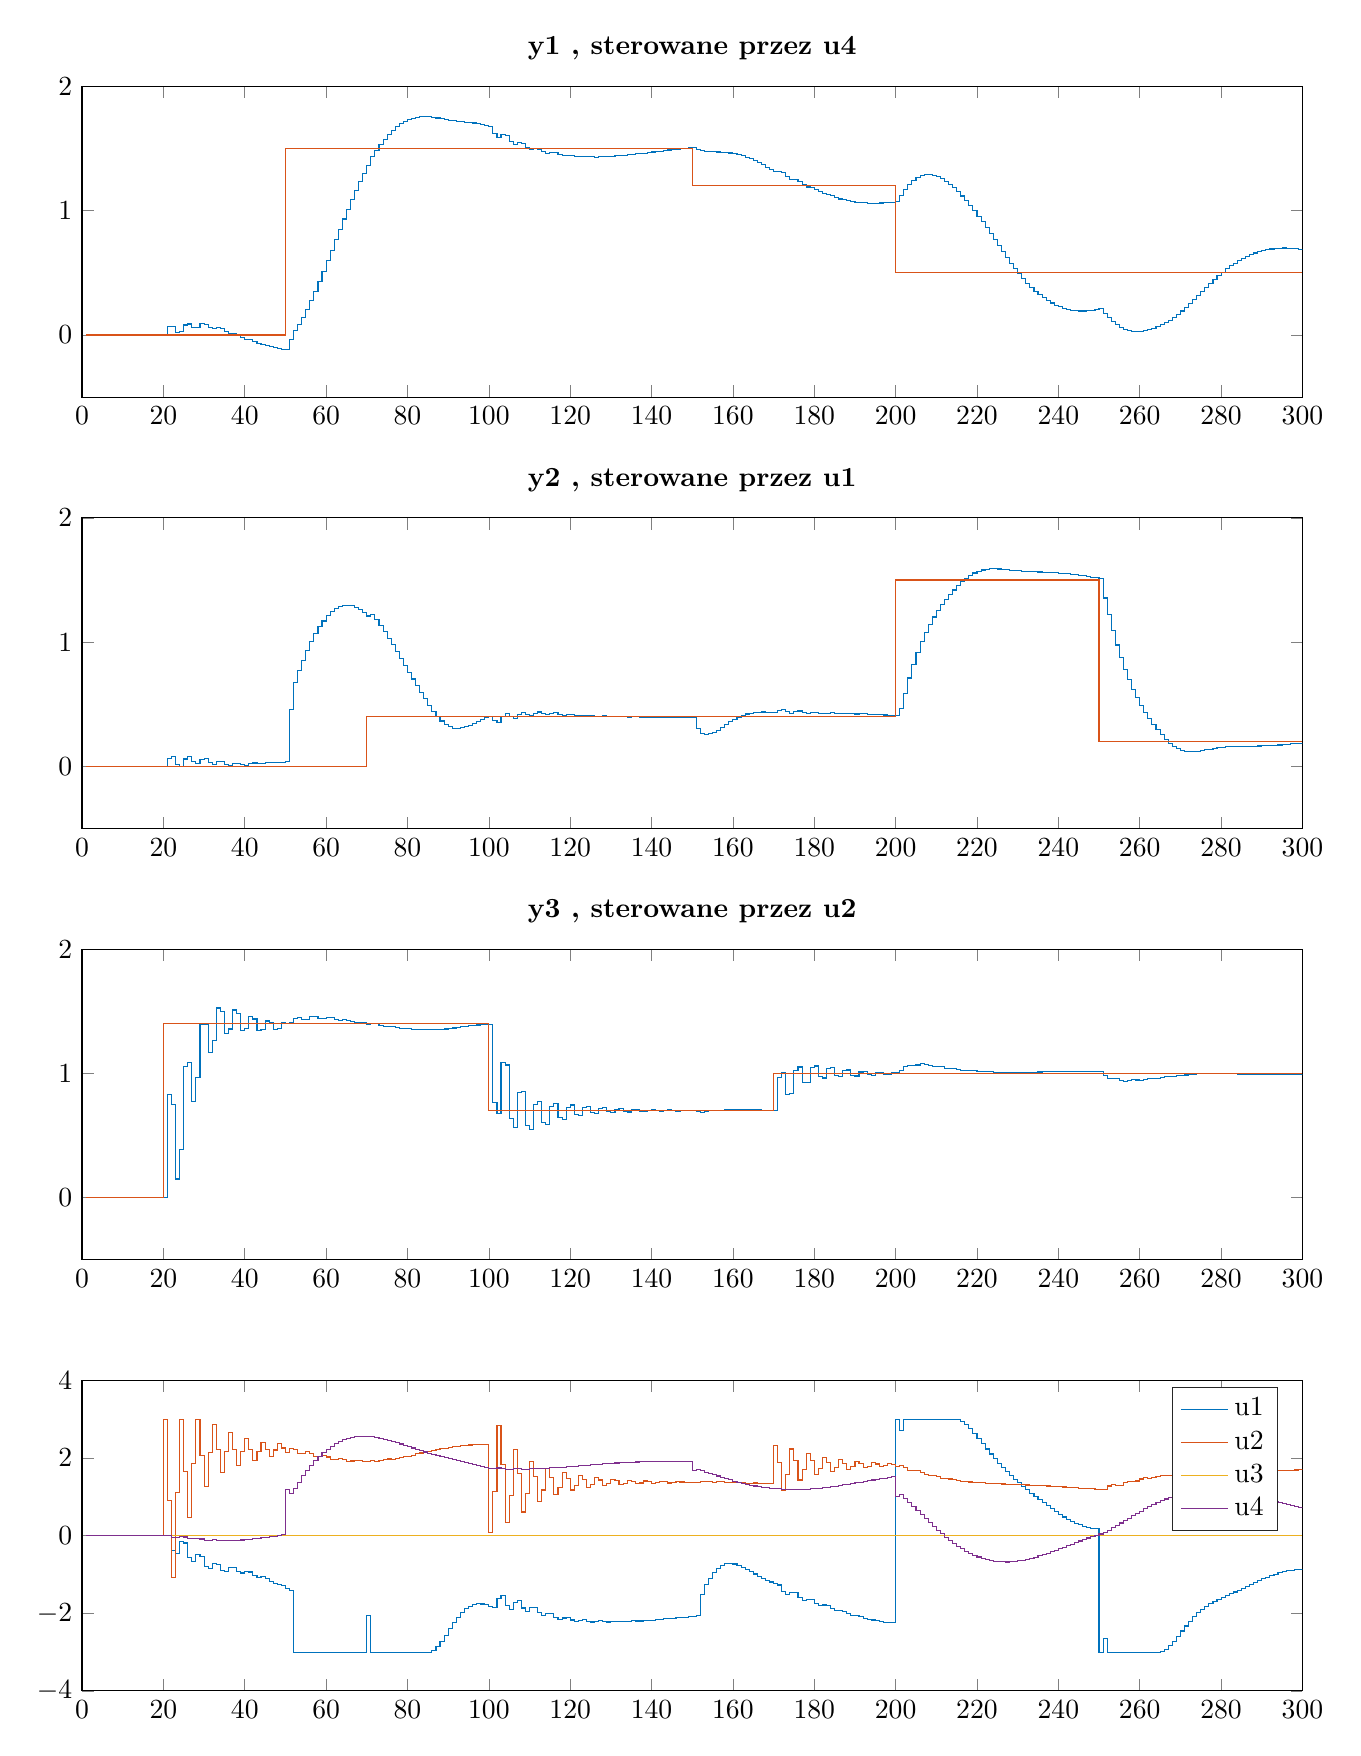
\begin{tikzpicture}

\begin{axis}[%
width=6.102in,
height=1.553in,
at={(1.024in,7.552in)},
scale only axis,
xmin=0,
xmax=300,
ymin=-0.5,
ymax=2,
axis background/.style={fill=white},
title style={font=\bfseries},
title={y1 , sterowane przez u4}
]
\addplot[const plot, color=mycolor1, forget plot] table[row sep=crcr] {%
1	0\\
2	0\\
3	0\\
4	0\\
5	0\\
6	0\\
7	0\\
8	0\\
9	0\\
10	0\\
11	0\\
12	0\\
13	0\\
14	0\\
15	0\\
16	0\\
17	0\\
18	0\\
19	0\\
20	0\\
21	0.0663597650785785\\
22	0.071588966531205\\
23	0.0214703350529014\\
24	0.0277809102800297\\
25	0.0802032921412371\\
26	0.0886880174096908\\
27	0.0584992546402986\\
28	0.0613448013208558\\
29	0.0898456197515564\\
30	0.0873329387617637\\
31	0.0592713485291592\\
32	0.0521035126344892\\
33	0.0621764461767634\\
34	0.0520037262907819\\
35	0.024792878929729\\
36	0.0119316650213101\\
37	0.011846667472554\\
38	-0.000525537291249014\\
39	-0.0236618232788303\\
40	-0.036617881719312\\
41	-0.0400567839917855\\
42	-0.0508663571779767\\
43	-0.0685366324532259\\
44	-0.0791482088307001\\
45	-0.0828932887621355\\
46	-0.0911241779652337\\
47	-0.103803989997499\\
48	-0.111644005261704\\
49	-0.114558771069335\\
50	-0.120132311301967\\
51	-0.0384241903643527\\
52	0.032379673025537\\
53	0.0826789319938879\\
54	0.138601168998581\\
55	0.203437739567975\\
56	0.276120209121537\\
57	0.352568141847555\\
58	0.431165579411588\\
59	0.51320305713262\\
60	0.598128889152364\\
61	0.683121987578111\\
62	0.766972116478558\\
63	0.850463138411822\\
64	0.933211540056068\\
65	1.0133298152386\\
66	1.09000378649255\\
67	1.16378643953244\\
68	1.23449475643724\\
69	1.30095031600424\\
70	1.36268973818417\\
71	1.43562240197006\\
72	1.48837602243693\\
73	1.53468170658714\\
74	1.5765748141534\\
75	1.61445206276592\\
76	1.64750287808489\\
77	1.675357081012\\
78	1.69884648469341\\
79	1.71853306169124\\
80	1.73404574486282\\
81	1.74527072186294\\
82	1.75289578658975\\
83	1.75743678793503\\
84	1.75877951390067\\
85	1.75696462280433\\
86	1.75256196432773\\
87	1.74669174822207\\
88	1.74028667622215\\
89	1.73398999622061\\
90	1.72840076117609\\
91	1.72379284414538\\
92	1.71994020867744\\
93	1.71648473184955\\
94	1.71320777895422\\
95	1.70983572122112\\
96	1.70590741950269\\
97	1.70101086958093\\
98	1.69495655782337\\
99	1.68762951424821\\
100	1.67887133733742\\
101	1.61828651504803\\
102	1.59066251864766\\
103	1.61043776532464\\
104	1.60410735872962\\
105	1.55859434400741\\
106	1.53512856696749\\
107	1.54575499555729\\
108	1.54071660509014\\
109	1.50959076166619\\
110	1.49288838991384\\
111	1.49950718423006\\
112	1.49629162739315\\
113	1.47542759679449\\
114	1.46379379232844\\
115	1.46798091270304\\
116	1.46600231971864\\
117	1.452149719336\\
118	1.44429645784753\\
119	1.44730344586528\\
120	1.44660983091803\\
121	1.43807092064744\\
122	1.43354471310947\\
123	1.43655710733007\\
124	1.43744388491126\\
125	1.43318794902451\\
126	1.43162451050207\\
127	1.43527165071781\\
128	1.43770239611309\\
129	1.43672388618418\\
130	1.43750089102939\\
131	1.44181901998521\\
132	1.44540603485246\\
133	1.44668042553996\\
134	1.44904603573248\\
135	1.45376712671556\\
136	1.45800890123242\\
137	1.4606402788621\\
138	1.4639046274313\\
139	1.46869503517458\\
140	1.47313246957541\\
141	1.47641187139164\\
142	1.48000986711998\\
143	1.48455422486015\\
144	1.48879937215979\\
145	1.49217384524502\\
146	1.4956479749595\\
147	1.4996613439843\\
148	1.5033890176703\\
149	1.50642758338992\\
150	1.5094151463872\\
151	1.49464323937136\\
152	1.48244878327275\\
153	1.47814771135691\\
154	1.47636979877366\\
155	1.47465127952011\\
156	1.4728569724722\\
157	1.47119726680307\\
158	1.46892828961085\\
159	1.46502454400638\\
160	1.45925114072233\\
161	1.45180717043072\\
162	1.44250221234394\\
163	1.43102317617646\\
164	1.41758064335956\\
165	1.40266485621727\\
166	1.3864765575827\\
167	1.36907940092665\\
168	1.35082777040329\\
169	1.33221185170362\\
170	1.31347636196393\\
171	1.31628655972648\\
172	1.30459948214628\\
173	1.27261098043877\\
174	1.25200582438978\\
175	1.24846939309786\\
176	1.23597099251266\\
177	1.20960604142118\\
178	1.19081140065285\\
179	1.18408684929313\\
180	1.17218350220721\\
181	1.15143200114558\\
182	1.13608920972148\\
183	1.12949700165384\\
184	1.12018287495045\\
185	1.10539320706307\\
186	1.09455969404296\\
187	1.0901012766365\\
188	1.08436667521381\\
189	1.07529863766078\\
190	1.06912216177135\\
191	1.06757215137504\\
192	1.06554762938385\\
193	1.06152914853695\\
194	1.05962118992586\\
195	1.0610598177652\\
196	1.06244319484083\\
197	1.062654464653\\
198	1.06439023674205\\
199	1.06851834260536\\
200	1.07276159473548\\
201	1.12044470897319\\
202	1.16822580489551\\
203	1.2103833758705\\
204	1.24255109247702\\
205	1.26654471553171\\
206	1.28310589920262\\
207	1.29154851577628\\
208	1.29227393599343\\
209	1.28687442025557\\
210	1.27610654626249\\
211	1.25977366544284\\
212	1.23835942764966\\
213	1.21312094596422\\
214	1.18474396931427\\
215	1.15324652303599\\
216	1.11891199250684\\
217	1.08207088845727\\
218	1.04275831446627\\
219	1.00075494467218\\
220	0.95628126171962\\
221	0.910044879208603\\
222	0.862599755564788\\
223	0.814224364383954\\
224	0.765389141157207\\
225	0.716815017542266\\
226	0.669050247917767\\
227	0.622383114851849\\
228	0.577161387273905\\
229	0.533850919969231\\
230	0.492766713180701\\
231	0.454020271855163\\
232	0.417742785418878\\
233	0.384138688473561\\
234	0.353314238224641\\
235	0.325243354834714\\
236	0.299919175749749\\
237	0.277394874133391\\
238	0.257670041120347\\
239	0.240664149536224\\
240	0.226315539713072\\
241	0.214608947124734\\
242	0.205497985185168\\
243	0.198883496068769\\
244	0.194677431130066\\
245	0.192821361815006\\
246	0.193234127310433\\
247	0.195795610832059\\
248	0.200388969669471\\
249	0.206914268063363\\
250	0.215254341087745\\
251	0.173362503226387\\
252	0.14037964840776\\
253	0.109869290413553\\
254	0.0846409392328157\\
255	0.0632710903495519\\
256	0.0467948657306896\\
257	0.0362336724140592\\
258	0.030235840894767\\
259	0.0274272488271611\\
260	0.0283324231545953\\
261	0.0334798298677465\\
262	0.0418328982358961\\
263	0.0523351208058711\\
264	0.0652115352878317\\
265	0.0807249878243572\\
266	0.09832712706764\\
267	0.117896040051625\\
268	0.140077740771137\\
269	0.165308782515833\\
270	0.193077058411571\\
271	0.222660896149656\\
272	0.253844662400368\\
273	0.286421133836625\\
274	0.319674022960168\\
275	0.352841012495977\\
276	0.385596430167763\\
277	0.417721525388726\\
278	0.44873650545857\\
279	0.478184146070735\\
280	0.50594158446268\\
281	0.531990805505586\\
282	0.556152867546036\\
283	0.578259556979573\\
284	0.598357112150136\\
285	0.616551683108629\\
286	0.632824773428667\\
287	0.647142742873\\
288	0.659596520575667\\
289	0.670303821980598\\
290	0.679286534908954\\
291	0.686544532285615\\
292	0.692154344180791\\
293	0.696209357954433\\
294	0.698739205950859\\
295	0.699759399456544\\
296	0.699340009194774\\
297	0.697568200813812\\
298	0.694493768533109\\
299	0.690160857456076\\
300	0.684654065639683\\
};
\addplot[const plot, color=mycolor2, forget plot] table[row sep=crcr] {%
1	0\\
2	0\\
3	0\\
4	0\\
5	0\\
6	0\\
7	0\\
8	0\\
9	0\\
10	0\\
11	0\\
12	0\\
13	0\\
14	0\\
15	0\\
16	0\\
17	0\\
18	0\\
19	0\\
20	0\\
21	0\\
22	0\\
23	0\\
24	0\\
25	0\\
26	0\\
27	0\\
28	0\\
29	0\\
30	0\\
31	0\\
32	0\\
33	0\\
34	0\\
35	0\\
36	0\\
37	0\\
38	0\\
39	0\\
40	0\\
41	0\\
42	0\\
43	0\\
44	0\\
45	0\\
46	0\\
47	0\\
48	0\\
49	0\\
50	1.5\\
51	1.5\\
52	1.5\\
53	1.5\\
54	1.5\\
55	1.5\\
56	1.5\\
57	1.5\\
58	1.5\\
59	1.5\\
60	1.5\\
61	1.5\\
62	1.5\\
63	1.5\\
64	1.5\\
65	1.5\\
66	1.5\\
67	1.5\\
68	1.5\\
69	1.5\\
70	1.5\\
71	1.5\\
72	1.5\\
73	1.5\\
74	1.5\\
75	1.5\\
76	1.5\\
77	1.5\\
78	1.5\\
79	1.5\\
80	1.5\\
81	1.5\\
82	1.5\\
83	1.5\\
84	1.5\\
85	1.5\\
86	1.5\\
87	1.5\\
88	1.5\\
89	1.5\\
90	1.5\\
91	1.5\\
92	1.5\\
93	1.5\\
94	1.5\\
95	1.5\\
96	1.5\\
97	1.5\\
98	1.5\\
99	1.5\\
100	1.5\\
101	1.5\\
102	1.5\\
103	1.5\\
104	1.5\\
105	1.5\\
106	1.5\\
107	1.5\\
108	1.5\\
109	1.5\\
110	1.5\\
111	1.5\\
112	1.5\\
113	1.5\\
114	1.5\\
115	1.5\\
116	1.5\\
117	1.5\\
118	1.5\\
119	1.5\\
120	1.5\\
121	1.5\\
122	1.5\\
123	1.5\\
124	1.5\\
125	1.5\\
126	1.5\\
127	1.5\\
128	1.5\\
129	1.5\\
130	1.5\\
131	1.5\\
132	1.5\\
133	1.5\\
134	1.5\\
135	1.5\\
136	1.5\\
137	1.5\\
138	1.5\\
139	1.5\\
140	1.5\\
141	1.5\\
142	1.5\\
143	1.5\\
144	1.5\\
145	1.5\\
146	1.5\\
147	1.5\\
148	1.5\\
149	1.5\\
150	1.2\\
151	1.2\\
152	1.2\\
153	1.2\\
154	1.2\\
155	1.2\\
156	1.2\\
157	1.2\\
158	1.2\\
159	1.2\\
160	1.2\\
161	1.2\\
162	1.2\\
163	1.2\\
164	1.2\\
165	1.2\\
166	1.2\\
167	1.2\\
168	1.2\\
169	1.2\\
170	1.2\\
171	1.2\\
172	1.2\\
173	1.2\\
174	1.2\\
175	1.2\\
176	1.2\\
177	1.2\\
178	1.2\\
179	1.2\\
180	1.2\\
181	1.2\\
182	1.2\\
183	1.2\\
184	1.2\\
185	1.2\\
186	1.2\\
187	1.2\\
188	1.2\\
189	1.2\\
190	1.2\\
191	1.2\\
192	1.2\\
193	1.2\\
194	1.2\\
195	1.2\\
196	1.2\\
197	1.2\\
198	1.2\\
199	1.2\\
200	0.5\\
201	0.5\\
202	0.5\\
203	0.5\\
204	0.5\\
205	0.5\\
206	0.5\\
207	0.5\\
208	0.5\\
209	0.5\\
210	0.5\\
211	0.5\\
212	0.5\\
213	0.5\\
214	0.5\\
215	0.5\\
216	0.5\\
217	0.5\\
218	0.5\\
219	0.5\\
220	0.5\\
221	0.5\\
222	0.5\\
223	0.5\\
224	0.5\\
225	0.5\\
226	0.5\\
227	0.5\\
228	0.5\\
229	0.5\\
230	0.5\\
231	0.5\\
232	0.5\\
233	0.5\\
234	0.5\\
235	0.5\\
236	0.5\\
237	0.5\\
238	0.5\\
239	0.5\\
240	0.5\\
241	0.5\\
242	0.5\\
243	0.5\\
244	0.5\\
245	0.5\\
246	0.5\\
247	0.5\\
248	0.5\\
249	0.5\\
250	0.5\\
251	0.5\\
252	0.5\\
253	0.5\\
254	0.5\\
255	0.5\\
256	0.5\\
257	0.5\\
258	0.5\\
259	0.5\\
260	0.5\\
261	0.5\\
262	0.5\\
263	0.5\\
264	0.5\\
265	0.5\\
266	0.5\\
267	0.5\\
268	0.5\\
269	0.5\\
270	0.5\\
271	0.5\\
272	0.5\\
273	0.5\\
274	0.5\\
275	0.5\\
276	0.5\\
277	0.5\\
278	0.5\\
279	0.5\\
280	0.5\\
281	0.5\\
282	0.5\\
283	0.5\\
284	0.5\\
285	0.5\\
286	0.5\\
287	0.5\\
288	0.5\\
289	0.5\\
290	0.5\\
291	0.5\\
292	0.5\\
293	0.5\\
294	0.5\\
295	0.5\\
296	0.5\\
297	0.5\\
298	0.5\\
299	0.5\\
300	0.5\\
};
\end{axis}

\begin{axis}[%
width=6.102in,
height=1.553in,
at={(1.024in,5.395in)},
scale only axis,
xmin=0,
xmax=300,
ymin=-0.5,
ymax=2,
axis background/.style={fill=white},
title style={font=\bfseries},
title={y2 , sterowane przez u1}
]
\addplot[const plot, color=mycolor1, forget plot] table[row sep=crcr] {%
1	0\\
2	0\\
3	0\\
4	0\\
5	0\\
6	0\\
7	0\\
8	0\\
9	0\\
10	0\\
11	0\\
12	0\\
13	0\\
14	0\\
15	0\\
16	0\\
17	0\\
18	0\\
19	0\\
20	0\\
21	0.0612158143362928\\
22	0.0770823080206103\\
23	0.0141649373921767\\
24	0.00164753617900343\\
25	0.059183717622069\\
26	0.0768041784430214\\
27	0.0363662346990625\\
28	0.025728430974402\\
29	0.0573890333525462\\
30	0.0617207374019321\\
31	0.0295948384874689\\
32	0.0181406180455044\\
33	0.035940862658433\\
34	0.0371158347661954\\
35	0.0148498214800161\\
36	0.00716916637898277\\
37	0.020498212823193\\
38	0.0240285706828503\\
39	0.0121638650178715\\
40	0.00988336064787799\\
41	0.0217848112732074\\
42	0.0271399830504687\\
43	0.0215424293324654\\
44	0.0214804750084914\\
45	0.030371896954922\\
46	0.0344490567741641\\
47	0.0304971130445764\\
48	0.0295533751785456\\
49	0.034272148065868\\
50	0.0356276075890335\\
51	0.458900988037706\\
52	0.673722797234978\\
53	0.771823193494731\\
54	0.854207726627001\\
55	0.932250626558587\\
56	1.00458579111018\\
57	1.06839208527864\\
58	1.12283723626762\\
59	1.17026491063747\\
60	1.21138714470496\\
61	1.24421460843472\\
62	1.26810387348595\\
63	1.28472153238748\\
64	1.29477362193287\\
65	1.29720062625534\\
66	1.29183748196664\\
67	1.28008263316688\\
68	1.26272026670416\\
69	1.23934321944417\\
70	1.21011104404965\\
71	1.22215007373545\\
72	1.18214805877138\\
73	1.13335593323976\\
74	1.08370912240277\\
75	1.03274043700721\\
76	0.979923774231826\\
77	0.9251271619634\\
78	0.869483718542474\\
79	0.813961978591989\\
80	0.75845993424651\\
81	0.70296309089156\\
82	0.648287036003435\\
83	0.59513185841718\\
84	0.543464354930274\\
85	0.493282011468266\\
86	0.44512147626414\\
87	0.401414566972582\\
88	0.364780617619408\\
89	0.336663593250725\\
90	0.317686835966472\\
91	0.307683903656338\\
92	0.305582182656337\\
93	0.309890152481981\\
94	0.319205183129249\\
95	0.332128189162663\\
96	0.347105514859535\\
97	0.362709476106556\\
98	0.377928664844276\\
99	0.392043030236413\\
100	0.404434644560671\\
101	0.368271979428903\\
102	0.353224302262432\\
103	0.399984366396291\\
104	0.42728370295597\\
105	0.399474589318233\\
106	0.385484044699574\\
107	0.41627895788561\\
108	0.435631517229036\\
109	0.417246057735254\\
110	0.406618491058352\\
111	0.425687285903525\\
112	0.437453875870246\\
113	0.423539221077463\\
114	0.414035805777884\\
115	0.424443665769001\\
116	0.430506309847084\\
117	0.419460273406034\\
118	0.411197597626685\\
119	0.416597156954497\\
120	0.419716815252746\\
121	0.411641977295027\\
122	0.40543792606624\\
123	0.408647666514467\\
124	0.410742142042736\\
125	0.405461022056089\\
126	0.401341676588335\\
127	0.403582960003319\\
128	0.405229027504873\\
129	0.401900218380646\\
130	0.399180935120055\\
131	0.400667560304617\\
132	0.401790965042152\\
133	0.399518661342759\\
134	0.397521701838467\\
135	0.398303576719417\\
136	0.398882562294772\\
137	0.39717540385413\\
138	0.395601380675573\\
139	0.395903716475384\\
140	0.396139975242703\\
141	0.394878950157552\\
142	0.393709321432544\\
143	0.393836496554719\\
144	0.393990344001856\\
145	0.393182300807094\\
146	0.392448160976938\\
147	0.392614230255091\\
148	0.392846123207242\\
149	0.392458326667206\\
150	0.392122438507998\\
151	0.306896517138198\\
152	0.263792126711988\\
153	0.255210198388951\\
154	0.261353474778956\\
155	0.273860393526838\\
156	0.291174780741891\\
157	0.312410436955314\\
158	0.33538803502445\\
159	0.357582190469217\\
160	0.377668126508955\\
161	0.395312945390321\\
162	0.410029440098319\\
163	0.421226436117547\\
164	0.429018198014059\\
165	0.434075264027587\\
166	0.436842796158772\\
167	0.437535787176378\\
168	0.436669757255024\\
169	0.434978549586887\\
170	0.432906305021438\\
171	0.45051080290485\\
172	0.458165621960414\\
173	0.438830444178391\\
174	0.427513487588382\\
175	0.439487740013682\\
176	0.445329627415318\\
177	0.43197289504327\\
178	0.423560007680056\\
179	0.431273624394463\\
180	0.435609209494312\\
181	0.427228183246413\\
182	0.421957793447112\\
183	0.427570105646745\\
184	0.431131273155012\\
185	0.426024459991689\\
186	0.422623833518049\\
187	0.426337307650096\\
188	0.428630092444118\\
189	0.424879256565483\\
190	0.42192913761485\\
191	0.423585398675098\\
192	0.424267403325757\\
193	0.420792617920998\\
194	0.41770294588012\\
195	0.417688739750618\\
196	0.417116647099925\\
197	0.413801847212633\\
198	0.410751872158943\\
199	0.409852116290798\\
200	0.408727041347679\\
201	0.462785613958046\\
202	0.588393897444077\\
203	0.711411532512483\\
204	0.820029196605712\\
205	0.91630259344573\\
206	1.00226959662259\\
207	1.07787071729238\\
208	1.14394411707592\\
209	1.20268472258336\\
210	1.25550408908925\\
211	1.30261318204527\\
212	1.3447252569535\\
213	1.38338912450644\\
214	1.41959225829759\\
215	1.45347472859595\\
216	1.48500364440118\\
217	1.51333538096919\\
218	1.53755494691364\\
219	1.55682168430447\\
220	1.57100906624122\\
221	1.58082304525614\\
222	1.5869994084658\\
223	1.58994754090158\\
224	1.59024305816823\\
225	1.58880183615492\\
226	1.58637467220648\\
227	1.58331787299799\\
228	1.5799495585012\\
229	1.57671262940497\\
230	1.57387803278394\\
231	1.57141772630625\\
232	1.56926801175952\\
233	1.56746679957665\\
234	1.56597422985386\\
235	1.56459319166754\\
236	1.56314773978358\\
237	1.56157873811831\\
238	1.55982230876281\\
239	1.55774748626507\\
240	1.55526624903123\\
241	1.55239171521529\\
242	1.54915007493748\\
243	1.54552939561447\\
244	1.54154567033413\\
245	1.5372783082543\\
246	1.53280851296346\\
247	1.52818137648891\\
248	1.52344813776181\\
249	1.51869091929183\\
250	1.51398291143466\\
251	1.35494248365363\\
252	1.2204637662935\\
253	1.09240883117929\\
254	0.977154656572344\\
255	0.873023030859801\\
256	0.779228806234063\\
257	0.696033002465276\\
258	0.621422428032147\\
259	0.553157701795761\\
260	0.491104159618324\\
261	0.435490953858181\\
262	0.384976575883714\\
263	0.338041688151623\\
264	0.2945696876666\\
265	0.254715618543033\\
266	0.218248890730221\\
267	0.186125688505145\\
268	0.159924162753655\\
269	0.140631838178779\\
270	0.127744128634345\\
271	0.120098696248776\\
272	0.117002299716631\\
273	0.117882576446345\\
274	0.12157539745529\\
275	0.126767484162002\\
276	0.132721619050359\\
277	0.139025707725552\\
278	0.145061527973188\\
279	0.150233864157501\\
280	0.154409225203934\\
281	0.157713179311998\\
282	0.16013306694246\\
283	0.161633285893154\\
284	0.16243172015606\\
285	0.162859541748183\\
286	0.163088430095207\\
287	0.163203393137433\\
288	0.163396004667003\\
289	0.163884944071903\\
290	0.164743093253372\\
291	0.16595394002963\\
292	0.16755337544375\\
293	0.16958993797207\\
294	0.172016597432235\\
295	0.17473230724756\\
296	0.177682212542466\\
297	0.180835995429059\\
298	0.184115940030859\\
299	0.18742261188182\\
300	0.190701049557718\\
};
\addplot[const plot, color=mycolor2, forget plot] table[row sep=crcr] {%
1	0\\
2	0\\
3	0\\
4	0\\
5	0\\
6	0\\
7	0\\
8	0\\
9	0\\
10	0\\
11	0\\
12	0\\
13	0\\
14	0\\
15	0\\
16	0\\
17	0\\
18	0\\
19	0\\
20	0\\
21	0\\
22	0\\
23	0\\
24	0\\
25	0\\
26	0\\
27	0\\
28	0\\
29	0\\
30	0\\
31	0\\
32	0\\
33	0\\
34	0\\
35	0\\
36	0\\
37	0\\
38	0\\
39	0\\
40	0\\
41	0\\
42	0\\
43	0\\
44	0\\
45	0\\
46	0\\
47	0\\
48	0\\
49	0\\
50	0\\
51	0\\
52	0\\
53	0\\
54	0\\
55	0\\
56	0\\
57	0\\
58	0\\
59	0\\
60	0\\
61	0\\
62	0\\
63	0\\
64	0\\
65	0\\
66	0\\
67	0\\
68	0\\
69	0\\
70	0.4\\
71	0.4\\
72	0.4\\
73	0.4\\
74	0.4\\
75	0.4\\
76	0.4\\
77	0.4\\
78	0.4\\
79	0.4\\
80	0.4\\
81	0.4\\
82	0.4\\
83	0.4\\
84	0.4\\
85	0.4\\
86	0.4\\
87	0.4\\
88	0.4\\
89	0.4\\
90	0.4\\
91	0.4\\
92	0.4\\
93	0.4\\
94	0.4\\
95	0.4\\
96	0.4\\
97	0.4\\
98	0.4\\
99	0.4\\
100	0.4\\
101	0.4\\
102	0.4\\
103	0.4\\
104	0.4\\
105	0.4\\
106	0.4\\
107	0.4\\
108	0.4\\
109	0.4\\
110	0.4\\
111	0.4\\
112	0.4\\
113	0.4\\
114	0.4\\
115	0.4\\
116	0.4\\
117	0.4\\
118	0.4\\
119	0.4\\
120	0.4\\
121	0.4\\
122	0.4\\
123	0.4\\
124	0.4\\
125	0.4\\
126	0.4\\
127	0.4\\
128	0.4\\
129	0.4\\
130	0.4\\
131	0.4\\
132	0.4\\
133	0.4\\
134	0.4\\
135	0.4\\
136	0.4\\
137	0.4\\
138	0.4\\
139	0.4\\
140	0.4\\
141	0.4\\
142	0.4\\
143	0.4\\
144	0.4\\
145	0.4\\
146	0.4\\
147	0.4\\
148	0.4\\
149	0.4\\
150	0.4\\
151	0.4\\
152	0.4\\
153	0.4\\
154	0.4\\
155	0.4\\
156	0.4\\
157	0.4\\
158	0.4\\
159	0.4\\
160	0.4\\
161	0.4\\
162	0.4\\
163	0.4\\
164	0.4\\
165	0.4\\
166	0.4\\
167	0.4\\
168	0.4\\
169	0.4\\
170	0.4\\
171	0.4\\
172	0.4\\
173	0.4\\
174	0.4\\
175	0.4\\
176	0.4\\
177	0.4\\
178	0.4\\
179	0.4\\
180	0.4\\
181	0.4\\
182	0.4\\
183	0.4\\
184	0.4\\
185	0.4\\
186	0.4\\
187	0.4\\
188	0.4\\
189	0.4\\
190	0.4\\
191	0.4\\
192	0.4\\
193	0.4\\
194	0.4\\
195	0.4\\
196	0.4\\
197	0.4\\
198	0.4\\
199	0.4\\
200	1.5\\
201	1.5\\
202	1.5\\
203	1.5\\
204	1.5\\
205	1.5\\
206	1.5\\
207	1.5\\
208	1.5\\
209	1.5\\
210	1.5\\
211	1.5\\
212	1.5\\
213	1.5\\
214	1.5\\
215	1.5\\
216	1.5\\
217	1.5\\
218	1.5\\
219	1.5\\
220	1.5\\
221	1.5\\
222	1.5\\
223	1.5\\
224	1.5\\
225	1.5\\
226	1.5\\
227	1.5\\
228	1.5\\
229	1.5\\
230	1.5\\
231	1.5\\
232	1.5\\
233	1.5\\
234	1.5\\
235	1.5\\
236	1.5\\
237	1.5\\
238	1.5\\
239	1.5\\
240	1.5\\
241	1.5\\
242	1.5\\
243	1.5\\
244	1.5\\
245	1.5\\
246	1.5\\
247	1.5\\
248	1.5\\
249	1.5\\
250	0.2\\
251	0.2\\
252	0.2\\
253	0.2\\
254	0.2\\
255	0.2\\
256	0.2\\
257	0.2\\
258	0.2\\
259	0.2\\
260	0.2\\
261	0.2\\
262	0.2\\
263	0.2\\
264	0.2\\
265	0.2\\
266	0.2\\
267	0.2\\
268	0.2\\
269	0.2\\
270	0.2\\
271	0.2\\
272	0.2\\
273	0.2\\
274	0.2\\
275	0.2\\
276	0.2\\
277	0.2\\
278	0.2\\
279	0.2\\
280	0.2\\
281	0.2\\
282	0.2\\
283	0.2\\
284	0.2\\
285	0.2\\
286	0.2\\
287	0.2\\
288	0.2\\
289	0.2\\
290	0.2\\
291	0.2\\
292	0.2\\
293	0.2\\
294	0.2\\
295	0.2\\
296	0.2\\
297	0.2\\
298	0.2\\
299	0.2\\
300	0.2\\
};
\end{axis}

\begin{axis}[%
width=6.102in,
height=1.553in,
at={(1.024in,3.239in)},
scale only axis,
xmin=0,
xmax=300,
ymin=-0.5,
ymax=2,
axis background/.style={fill=white},
title style={font=\bfseries},
title={y3 , sterowane przez u2}
]
\addplot[const plot, color=mycolor1, forget plot] table[row sep=crcr] {%
1	0\\
2	0\\
3	0\\
4	0\\
5	0\\
6	0\\
7	0\\
8	0\\
9	0\\
10	0\\
11	0\\
12	0\\
13	0\\
14	0\\
15	0\\
16	0\\
17	0\\
18	0\\
19	0\\
20	0\\
21	0.82628561460347\\
22	0.749053243317543\\
23	0.149745556121401\\
24	0.386983620233136\\
25	1.05502658492221\\
26	1.08833942120088\\
27	0.774674269910132\\
28	0.966483758822896\\
29	1.39477627412445\\
30	1.39331491320797\\
31	1.16886305161047\\
32	1.26695834458507\\
33	1.52594541081074\\
34	1.50049313882623\\
35	1.32104091867572\\
36	1.35708770955616\\
37	1.51011056088418\\
38	1.48025492059295\\
39	1.34744861126852\\
40	1.36014237669592\\
41	1.45769254469778\\
42	1.43750470608221\\
43	1.34758676040769\\
44	1.35460399056158\\
45	1.42145000515888\\
46	1.41140333943733\\
47	1.35304787834989\\
48	1.35829270652551\\
49	1.4048440133884\\
50	1.40069809271729\\
51	1.40667308600013\\
52	1.44304976863202\\
53	1.45294924353093\\
54	1.4346244534887\\
55	1.4351364578597\\
56	1.45618739986202\\
57	1.4595237118862\\
58	1.44364450366878\\
59	1.43996646289714\\
60	1.4501873698695\\
61	1.44891633794591\\
62	1.43480497805412\\
63	1.42879724462021\\
64	1.43238311142237\\
65	1.42869486509089\\
66	1.41658208233413\\
67	1.40998336733578\\
68	1.41011220030004\\
69	1.40575066047718\\
70	1.39595095389523\\
71	1.399004845076\\
72	1.39755019027717\\
73	1.38486939668442\\
74	1.37599884473148\\
75	1.37674100129031\\
76	1.37508034925938\\
77	1.36633846853679\\
78	1.36037445195763\\
79	1.36112550095166\\
80	1.36058148251696\\
81	1.35544448284362\\
82	1.35218574572292\\
83	1.35349657990032\\
84	1.35406010894347\\
85	1.3515791477323\\
86	1.35031616938842\\
87	1.35251149480793\\
88	1.35517973692506\\
89	1.35671823433891\\
90	1.35953713275814\\
91	1.36474463095697\\
92	1.37000311861771\\
93	1.37391258774275\\
94	1.37787529278575\\
95	1.38258743552312\\
96	1.38651519482297\\
97	1.38877287059162\\
98	1.39041617362844\\
99	1.39210483964304\\
100	1.39300797142851\\
101	0.766085276395419\\
102	0.674530487667892\\
103	1.08768359205897\\
104	1.06683991630417\\
105	0.63462939264065\\
106	0.563977569220786\\
107	0.848048125490286\\
108	0.855446632413468\\
109	0.58361834462505\\
110	0.54721853560947\\
111	0.752395981138147\\
112	0.776272252648617\\
113	0.606740440996675\\
114	0.587526929354671\\
115	0.730987112498324\\
116	0.754948437328092\\
117	0.645010446844477\\
118	0.631025604771374\\
119	0.727034563073903\\
120	0.745023099937055\\
121	0.671194894185022\\
122	0.659118783642683\\
123	0.721963797987196\\
124	0.734442132177753\\
125	0.684443137625322\\
126	0.67439616073639\\
127	0.715535418481661\\
128	0.724352954510659\\
129	0.690766798559797\\
130	0.683004436367139\\
131	0.710164696643858\\
132	0.716606400767516\\
133	0.694256882435906\\
134	0.68852744423397\\
135	0.706560341160099\\
136	0.711312254446895\\
137	0.69650518312552\\
138	0.692349261568379\\
139	0.704330037181068\\
140	0.707808030796758\\
141	0.698003995323262\\
142	0.69500413214617\\
143	0.70295034071899\\
144	0.70546650179439\\
145	0.698971238353747\\
146	0.696810304435649\\
147	0.702068161030614\\
148	0.703868538268409\\
149	0.69956050555899\\
150	0.698004856347322\\
151	0.692693816195437\\
152	0.687399849841675\\
153	0.691062072404329\\
154	0.697823851377444\\
155	0.698971613450935\\
156	0.698569794673833\\
157	0.703168013489116\\
158	0.708860033783222\\
159	0.709699043974895\\
160	0.708444944297286\\
161	0.709809839888537\\
162	0.711568797046209\\
163	0.709948235176252\\
164	0.706923291409122\\
165	0.705862057232177\\
166	0.705473399998297\\
167	0.70326741080413\\
168	0.700521581728144\\
169	0.699494183147857\\
170	0.699322059515325\\
171	0.966790800074657\\
172	1.00448283249395\\
173	0.827232777567132\\
174	0.836528609970941\\
175	1.02130851893315\\
176	1.05097477598154\\
177	0.929565373566837\\
178	0.927124575964177\\
179	1.04379410429567\\
180	1.05940224220351\\
181	0.972049956824133\\
182	0.962610920234133\\
183	1.03562651869646\\
184	1.04403736106664\\
185	0.983053079568669\\
186	0.973384903476656\\
187	1.02077647948579\\
188	1.02688808734997\\
189	0.986053319541166\\
190	0.978719330766926\\
191	1.010516443447\\
192	1.01574059352117\\
193	0.988988720128719\\
194	0.983876055805086\\
195	1.00540280035989\\
196	1.00974002668083\\
197	0.992234456247495\\
198	0.988624072833999\\
199	1.00309941103114\\
200	1.00646137971091\\
201	1.02484835641095\\
202	1.05310835360361\\
203	1.06613124177989\\
204	1.06410660410986\\
205	1.06718568611839\\
206	1.07586458744191\\
207	1.07462819772312\\
208	1.06411460504198\\
209	1.05822533794744\\
210	1.05773096151654\\
211	1.05234282577339\\
212	1.04222613942937\\
213	1.0364622350059\\
214	1.0354833593982\\
215	1.03220619064986\\
216	1.02630868358344\\
217	1.02326997587635\\
218	1.02306371697519\\
219	1.02095887585232\\
220	1.01677989909945\\
221	1.0143396211176\\
222	1.01384186457251\\
223	1.01223437614428\\
224	1.00940142527606\\
225	1.00792636081426\\
226	1.00800816040053\\
227	1.00758383058577\\
228	1.00648013109104\\
229	1.00636155862799\\
230	1.00733842984979\\
231	1.0079755438045\\
232	1.00807339518536\\
233	1.00870226074844\\
234	1.00993660427528\\
235	1.01080736536788\\
236	1.01115913103648\\
237	1.01171465045042\\
238	1.01255899358001\\
239	1.01306918629821\\
240	1.01315169436776\\
241	1.01331248624398\\
242	1.01364335402871\\
243	1.01374963708293\\
244	1.01357510982089\\
245	1.0134679555871\\
246	1.01350463747871\\
247	1.01342601151175\\
248	1.0131879594914\\
249	1.01301922852567\\
250	1.01297151102059\\
251	0.982507276770559\\
252	0.956101876422018\\
253	0.955836924919332\\
254	0.957503815348891\\
255	0.943464398396927\\
256	0.933113755416454\\
257	0.940407239258721\\
258	0.948814714717645\\
259	0.945916045360353\\
260	0.944211929258244\\
261	0.953121105209871\\
262	0.961816120451086\\
263	0.961959511970954\\
264	0.961892663405308\\
265	0.968183946435893\\
266	0.974015949285697\\
267	0.974266095692386\\
268	0.974763580737672\\
269	0.979927572158356\\
270	0.985066017557699\\
271	0.986430231853235\\
272	0.987663194741694\\
273	0.991687254968982\\
274	0.995368114917705\\
275	0.996111920937179\\
276	0.996325551797055\\
277	0.998086552430374\\
278	0.99943679579857\\
279	0.998693449059365\\
280	0.997521953616639\\
281	0.997436151719449\\
282	0.997231651923561\\
283	0.995804345551875\\
284	0.994270646441604\\
285	0.993678556214616\\
286	0.993240162783657\\
287	0.99217796042016\\
288	0.991189989214345\\
289	0.990957965046461\\
290	0.990933960229454\\
291	0.990549336969395\\
292	0.990225259606801\\
293	0.990400679571325\\
294	0.990699061818586\\
295	0.990717279079383\\
296	0.990719568755959\\
297	0.991003301912875\\
298	0.991325914375419\\
299	0.991417743015503\\
300	0.991456977598919\\
};
\addplot[const plot, color=mycolor2, forget plot] table[row sep=crcr] {%
1	0\\
2	0\\
3	0\\
4	0\\
5	0\\
6	0\\
7	0\\
8	0\\
9	0\\
10	0\\
11	0\\
12	0\\
13	0\\
14	0\\
15	0\\
16	0\\
17	0\\
18	0\\
19	0\\
20	1.4\\
21	1.4\\
22	1.4\\
23	1.4\\
24	1.4\\
25	1.4\\
26	1.4\\
27	1.4\\
28	1.4\\
29	1.4\\
30	1.4\\
31	1.4\\
32	1.4\\
33	1.4\\
34	1.4\\
35	1.4\\
36	1.4\\
37	1.4\\
38	1.4\\
39	1.4\\
40	1.4\\
41	1.4\\
42	1.4\\
43	1.4\\
44	1.4\\
45	1.4\\
46	1.4\\
47	1.4\\
48	1.4\\
49	1.4\\
50	1.4\\
51	1.4\\
52	1.4\\
53	1.4\\
54	1.4\\
55	1.4\\
56	1.4\\
57	1.4\\
58	1.4\\
59	1.4\\
60	1.4\\
61	1.4\\
62	1.4\\
63	1.4\\
64	1.4\\
65	1.4\\
66	1.4\\
67	1.4\\
68	1.4\\
69	1.4\\
70	1.4\\
71	1.4\\
72	1.4\\
73	1.4\\
74	1.4\\
75	1.4\\
76	1.4\\
77	1.4\\
78	1.4\\
79	1.4\\
80	1.4\\
81	1.4\\
82	1.4\\
83	1.4\\
84	1.4\\
85	1.4\\
86	1.4\\
87	1.4\\
88	1.4\\
89	1.4\\
90	1.4\\
91	1.4\\
92	1.4\\
93	1.4\\
94	1.4\\
95	1.4\\
96	1.4\\
97	1.4\\
98	1.4\\
99	1.4\\
100	0.7\\
101	0.7\\
102	0.7\\
103	0.7\\
104	0.7\\
105	0.7\\
106	0.7\\
107	0.7\\
108	0.7\\
109	0.7\\
110	0.7\\
111	0.7\\
112	0.7\\
113	0.7\\
114	0.7\\
115	0.7\\
116	0.7\\
117	0.7\\
118	0.7\\
119	0.7\\
120	0.7\\
121	0.7\\
122	0.7\\
123	0.7\\
124	0.7\\
125	0.7\\
126	0.7\\
127	0.7\\
128	0.7\\
129	0.7\\
130	0.7\\
131	0.7\\
132	0.7\\
133	0.7\\
134	0.7\\
135	0.7\\
136	0.7\\
137	0.7\\
138	0.7\\
139	0.7\\
140	0.7\\
141	0.7\\
142	0.7\\
143	0.7\\
144	0.7\\
145	0.7\\
146	0.7\\
147	0.7\\
148	0.7\\
149	0.7\\
150	0.7\\
151	0.7\\
152	0.7\\
153	0.7\\
154	0.7\\
155	0.7\\
156	0.7\\
157	0.7\\
158	0.7\\
159	0.7\\
160	0.7\\
161	0.7\\
162	0.7\\
163	0.7\\
164	0.7\\
165	0.7\\
166	0.7\\
167	0.7\\
168	0.7\\
169	0.7\\
170	1\\
171	1\\
172	1\\
173	1\\
174	1\\
175	1\\
176	1\\
177	1\\
178	1\\
179	1\\
180	1\\
181	1\\
182	1\\
183	1\\
184	1\\
185	1\\
186	1\\
187	1\\
188	1\\
189	1\\
190	1\\
191	1\\
192	1\\
193	1\\
194	1\\
195	1\\
196	1\\
197	1\\
198	1\\
199	1\\
200	1\\
201	1\\
202	1\\
203	1\\
204	1\\
205	1\\
206	1\\
207	1\\
208	1\\
209	1\\
210	1\\
211	1\\
212	1\\
213	1\\
214	1\\
215	1\\
216	1\\
217	1\\
218	1\\
219	1\\
220	1\\
221	1\\
222	1\\
223	1\\
224	1\\
225	1\\
226	1\\
227	1\\
228	1\\
229	1\\
230	1\\
231	1\\
232	1\\
233	1\\
234	1\\
235	1\\
236	1\\
237	1\\
238	1\\
239	1\\
240	1\\
241	1\\
242	1\\
243	1\\
244	1\\
245	1\\
246	1\\
247	1\\
248	1\\
249	1\\
250	1\\
251	1\\
252	1\\
253	1\\
254	1\\
255	1\\
256	1\\
257	1\\
258	1\\
259	1\\
260	1\\
261	1\\
262	1\\
263	1\\
264	1\\
265	1\\
266	1\\
267	1\\
268	1\\
269	1\\
270	1\\
271	1\\
272	1\\
273	1\\
274	1\\
275	1\\
276	1\\
277	1\\
278	1\\
279	1\\
280	1\\
281	1\\
282	1\\
283	1\\
284	1\\
285	1\\
286	1\\
287	1\\
288	1\\
289	1\\
290	1\\
291	1\\
292	1\\
293	1\\
294	1\\
295	1\\
296	1\\
297	1\\
298	1\\
299	1\\
300	1\\
};
\end{axis}

\begin{axis}[%
width=6.102in,
height=1.553in,
at={(1.024in,1.083in)},
scale only axis,
xmin=0,
xmax=300,
ymin=-4,
ymax=4,
axis background/.style={fill=white},
legend style={legend cell align=left, align=left, draw=white!15!black}
]
\addplot[const plot, color=mycolor1] table[row sep=crcr] {%
1	0\\
2	0\\
3	0\\
4	0\\
5	0\\
6	0\\
7	0\\
8	0\\
9	0\\
10	0\\
11	0\\
12	0\\
13	0\\
14	0\\
15	0\\
16	0\\
17	0\\
18	0\\
19	0\\
20	0\\
21	0\\
22	-0.383619103174101\\
23	-0.466724913106147\\
24	-0.149832744633868\\
25	-0.190944739893045\\
26	-0.573729367116005\\
27	-0.67100465478116\\
28	-0.491806374596189\\
29	-0.538331827510734\\
30	-0.788063329672431\\
31	-0.84107042238028\\
32	-0.715111712573202\\
33	-0.734193154049992\\
34	-0.888255597058826\\
35	-0.915059514431362\\
36	-0.823133655487146\\
37	-0.830426933418579\\
38	-0.935803561135927\\
39	-0.963931613176634\\
40	-0.915968979344448\\
41	-0.936879834380284\\
42	-1.02828887948818\\
43	-1.07185204998943\\
44	-1.06439241591362\\
45	-1.10168349387547\\
46	-1.18614283166945\\
47	-1.23796262069564\\
48	-1.25260572664499\\
49	-1.29367756337797\\
50	-1.36416302096224\\
51	-1.41080339477551\\
52	-3\\
53	-3\\
54	-3\\
55	-3\\
56	-3\\
57	-3\\
58	-3\\
59	-3\\
60	-3\\
61	-3\\
62	-3\\
63	-3\\
64	-3\\
65	-3\\
66	-3\\
67	-3\\
68	-3\\
69	-3\\
70	-2.05824397911662\\
71	-3\\
72	-3\\
73	-3\\
74	-3\\
75	-3\\
76	-3\\
77	-3\\
78	-3\\
79	-3\\
80	-3\\
81	-3\\
82	-3\\
83	-3\\
84	-3\\
85	-3\\
86	-2.95947779312416\\
87	-2.86233953734188\\
88	-2.72566173046024\\
89	-2.56790612534361\\
90	-2.40336124842415\\
91	-2.24497893276703\\
92	-2.10290581656696\\
93	-1.98265159487162\\
94	-1.8871205362541\\
95	-1.81845551323193\\
96	-1.77680921284469\\
97	-1.75949456310851\\
98	-1.7627896856209\\
99	-1.78347623185745\\
100	-1.81814710612686\\
101	-1.86260894491334\\
102	-1.62207585324967\\
103	-1.54333331312249\\
104	-1.79807173484427\\
105	-1.89431062986581\\
106	-1.71273951651513\\
107	-1.66885947114955\\
108	-1.864871191438\\
109	-1.95858064607329\\
110	-1.85990969460149\\
111	-1.84572175559662\\
112	-1.99104829805389\\
113	-2.06852523796443\\
114	-2.01243869180989\\
115	-2.00653303170427\\
116	-2.10567549316511\\
117	-2.15960704109398\\
118	-2.12136006200124\\
119	-2.11320131663105\\
120	-2.17518896650121\\
121	-2.20822907285174\\
122	-2.17892438870983\\
123	-2.16848804480181\\
124	-2.20577946833175\\
125	-2.22529948561102\\
126	-2.20317616223979\\
127	-2.19309275202862\\
128	-2.21551798296204\\
129	-2.22702456584556\\
130	-2.21050235733775\\
131	-2.20132123467767\\
132	-2.21389618587794\\
133	-2.21944766901068\\
134	-2.20579840497064\\
135	-2.19627802645311\\
136	-2.20106851336522\\
137	-2.20118392545382\\
138	-2.18806943869826\\
139	-2.17717088542316\\
140	-2.17571913442177\\
141	-2.17125424071778\\
142	-2.15782710314673\\
143	-2.14568700348299\\
144	-2.13996780211869\\
145	-2.13251042799823\\
146	-2.11918766006478\\
147	-2.10678965398355\\
148	-2.09893585982413\\
149	-2.09027565181936\\
150	-2.07793592905468\\
151	-2.06639593994397\\
152	-1.52234750509196\\
153	-1.26445015546366\\
154	-1.09802659827054\\
155	-0.957202480150037\\
156	-0.840887895118029\\
157	-0.761194176371535\\
158	-0.721467643420752\\
159	-0.714697457319616\\
160	-0.730867387895469\\
161	-0.764671525658488\\
162	-0.813332394996741\\
163	-0.871074645477107\\
164	-0.93106868246256\\
165	-0.990283778206668\\
166	-1.04819883687577\\
167	-1.10288441797967\\
168	-1.1519228384918\\
169	-1.19543464825832\\
170	-1.23511507108552\\
171	-1.27147300352691\\
172	-1.42898518826292\\
173	-1.5161359282708\\
174	-1.46027526629511\\
175	-1.47206588168681\\
176	-1.60189631088054\\
177	-1.67199698806856\\
178	-1.63938728191487\\
179	-1.65066781962503\\
180	-1.7438804477232\\
181	-1.80040649346515\\
182	-1.78842740547764\\
183	-1.80511351572721\\
184	-1.87799368711994\\
185	-1.92809077818132\\
186	-1.93189857855129\\
187	-1.95345816703338\\
188	-2.01233538530943\\
189	-2.05587835494083\\
190	-2.06687811768977\\
191	-2.08756438509226\\
192	-2.13190266154396\\
193	-2.16497373789182\\
194	-2.17446374634862\\
195	-2.18838494876807\\
196	-2.21684332679542\\
197	-2.23686592899243\\
198	-2.23983072740642\\
199	-2.24442369317313\\
200	3\\
201	2.69914137186679\\
202	3\\
203	3\\
204	3\\
205	3\\
206	3\\
207	3\\
208	3\\
209	3\\
210	3\\
211	3\\
212	3\\
213	3\\
214	3\\
215	2.99047038365164\\
216	2.94327557278427\\
217	2.86194001475429\\
218	2.75483587168155\\
219	2.63061019564625\\
220	2.49855001762327\\
221	2.36470695823901\\
222	2.23122707918936\\
223	2.10046017582453\\
224	1.97586818240801\\
225	1.85880323156549\\
226	1.74798363958453\\
227	1.64248546356694\\
228	1.54259171334731\\
229	1.44771844146297\\
230	1.35601448260288\\
231	1.26631536233408\\
232	1.17869388462203\\
233	1.09300530367557\\
234	1.00849600773406\\
235	0.925011772402145\\
236	0.843312527008105\\
237	0.764036775492754\\
238	0.687359476536018\\
239	0.613751047008312\\
240	0.54417990267495\\
241	0.479412624990522\\
242	0.419768058621311\\
243	0.365627463303017\\
244	0.317596996032761\\
245	0.276062726720111\\
246	0.241036674859659\\
247	0.21251520168215\\
248	0.190615567172699\\
249	0.175298609518039\\
250	-3\\
251	-2.65636259270282\\
252	-3\\
253	-3\\
254	-3\\
255	-3\\
256	-3\\
257	-3\\
258	-3\\
259	-3\\
260	-3\\
261	-3\\
262	-3\\
263	-3\\
264	-3\\
265	-2.9867268682007\\
266	-2.93262281935785\\
267	-2.84081866038598\\
268	-2.72219187858296\\
269	-2.59089369210727\\
270	-2.45848311631197\\
271	-2.32943030672503\\
272	-2.20579810389235\\
273	-2.09209163910619\\
274	-1.99189867401933\\
275	-1.90414201150298\\
276	-1.82620443785778\\
277	-1.75756632331008\\
278	-1.6978408219204\\
279	-1.64427969722601\\
280	-1.59378439554907\\
281	-1.54531940575515\\
282	-1.49855590742997\\
283	-1.45205178242396\\
284	-1.40442542356285\\
285	-1.35587297581349\\
286	-1.30718545651156\\
287	-1.25841469793642\\
288	-1.20955348510608\\
289	-1.16151443400706\\
290	-1.1154649487198\\
291	-1.07190697263837\\
292	-1.03111269808373\\
293	-0.99380372520971\\
294	-0.960744920982924\\
295	-0.932146737517407\\
296	-0.907971327133491\\
297	-0.888422007607129\\
298	-0.873708815281218\\
299	-0.863665076072694\\
300	-0.857960228350315\\
};
\addlegendentry{u1}

\addplot[const plot, color=mycolor2] table[row sep=crcr] {%
1	0\\
2	0\\
3	0\\
4	0\\
5	0\\
6	0\\
7	0\\
8	0\\
9	0\\
10	0\\
11	0\\
12	0\\
13	0\\
14	0\\
15	0\\
16	0\\
17	0\\
18	0\\
19	0\\
20	3\\
21	0.9\\
22	-1.08542824746128\\
23	1.10500538112319\\
24	3\\
25	1.65548813918388\\
26	0.465332822051297\\
27	1.86563874106266\\
28	3\\
29	2.06195172349696\\
30	1.27037814718098\\
31	2.13432446370043\\
32	2.86421283545535\\
33	2.21206788428769\\
34	1.63307133271092\\
35	2.17079264370652\\
36	2.65286124581355\\
37	2.21628427581326\\
38	1.81250973598\\
39	2.16053098914044\\
40	2.49231275356591\\
41	2.21172109164372\\
42	1.93999938814453\\
43	2.17186392729997\\
44	2.40496922046989\\
45	2.2285339509169\\
46	2.04801686850265\\
47	2.20363555871283\\
48	2.36749580608526\\
49	2.25721525316465\\
50	2.13726680894877\\
51	2.24142165816143\\
52	2.21336204229136\\
53	2.10375126730332\\
54	2.12280645482965\\
55	2.17568635049922\\
56	2.12006052946468\\
57	2.03510074776929\\
58	2.03826591776432\\
59	2.06678411257621\\
60	2.02515707681482\\
61	1.96459981616277\\
62	1.96407879892444\\
63	1.98294048575259\\
64	1.95684041060217\\
65	1.91877225431724\\
66	1.92173923278768\\
67	1.93938185153872\\
68	1.9283110686028\\
69	1.90970324780435\\
70	1.91907981800715\\
71	1.93933045451419\\
72	1.91183041806517\\
73	1.92316340598491\\
74	1.96269158042509\\
75	1.97372458874443\\
76	1.96557205365662\\
77	1.98408298522967\\
78	2.0216326188865\\
79	2.04036267705521\\
80	2.04580650868748\\
81	2.06851391611249\\
82	2.10383038692294\\
83	2.12642504179674\\
84	2.13955448361734\\
85	2.16359639263172\\
86	2.19575652018259\\
87	2.21910970351171\\
88	2.23429085451635\\
89	2.25375397107071\\
90	2.27650047024744\\
91	2.29205692804317\\
92	2.30100178935637\\
93	2.31195438537816\\
94	2.32476402673437\\
95	2.33274787972336\\
96	2.33642117952\\
97	2.34178652950868\\
98	2.34904700444878\\
99	2.35383518582061\\
100	0.0814255405325688\\
101	1.13581527443749\\
102	2.82861631115171\\
103	1.83928134625228\\
104	0.326158935692278\\
105	1.02636529464804\\
106	2.20594218689281\\
107	1.60382486935999\\
108	0.607303130033998\\
109	1.07737503232751\\
110	1.8978906652795\\
111	1.53072429669078\\
112	0.86748871288668\\
113	1.17404773096593\\
114	1.73464253553138\\
115	1.50465260456567\\
116	1.05621652138745\\
117	1.24976902572885\\
118	1.62751592579609\\
119	1.48058545814421\\
120	1.17507385712909\\
121	1.29511174739196\\
122	1.54851893984384\\
123	1.45451244050986\\
124	1.24655453098418\\
125	1.3207080745603\\
126	1.49094040914793\\
127	1.43137352611944\\
128	1.29037890430125\\
129	1.33623271845672\\
130	1.45084632009969\\
131	1.4135182860442\\
132	1.31822049757598\\
133	1.3465231314056\\
134	1.42373927384689\\
135	1.40053247012201\\
136	1.33620295659123\\
137	1.35354486168135\\
138	1.40551554282597\\
139	1.39115555368116\\
140	1.34773155904145\\
141	1.3582246124253\\
142	1.39313969954717\\
143	1.38427918626409\\
144	1.35495221597516\\
145	1.36119193926625\\
146	1.38460061670195\\
147	1.37914750587761\\
148	1.35933245188995\\
149	1.36296285854174\\
150	1.37863045018874\\
151	1.37528999192833\\
152	1.39043714582496\\
153	1.40067354807319\\
154	1.38448346711621\\
155	1.37430109437673\\
156	1.38518249989539\\
157	1.38929812834248\\
158	1.37426538230169\\
159	1.36337874723186\\
160	1.36760598780552\\
161	1.36851031015365\\
162	1.35734372797822\\
163	1.34945198845402\\
164	1.35245233032362\\
165	1.35406815623875\\
166	1.348005634075\\
167	1.34421527311514\\
168	1.34787072352927\\
169	1.35074898423582\\
170	2.32333558060571\\
171	1.87209309367694\\
172	1.15281440983638\\
173	1.58185738555502\\
174	2.23106271265879\\
175	1.9327347587092\\
176	1.43252741440419\\
177	1.69501763745476\\
178	2.12344332140854\\
179	1.92377442200437\\
180	1.57615457173962\\
181	1.73687012805429\\
182	2.02228021025117\\
183	1.89222752999786\\
184	1.65474330169823\\
185	1.75562600157156\\
186	1.94862792064702\\
187	1.86655439016578\\
188	1.70650296421375\\
189	1.77103515093053\\
190	1.90252731836251\\
191	1.85166658649061\\
192	1.74429832734841\\
193	1.78565584324402\\
194	1.87517743515724\\
195	1.84379548735979\\
196	1.77167021100688\\
197	1.79792631439345\\
198	1.85862385760328\\
199	1.83922923470672\\
200	1.79065158232202\\
201	1.80712615499149\\
202	1.75086172822044\\
203	1.6833665125389\\
204	1.6710079435495\\
205	1.6705681714397\\
206	1.624458577517\\
207	1.56881746917344\\
208	1.55226124468557\\
209	1.54664354260013\\
210	1.51269917277415\\
211	1.47341469301173\\
212	1.46107190055692\\
213	1.45700344680199\\
214	1.43438969377555\\
215	1.40781211315067\\
216	1.39876348066828\\
217	1.39527294581253\\
218	1.38019938993604\\
219	1.36315732801242\\
220	1.35805368537187\\
221	1.35694623964676\\
222	1.34812924003232\\
223	1.33769658228136\\
224	1.33500447429667\\
225	1.33487939968978\\
226	1.32930674481619\\
227	1.32212758683005\\
228	1.31966617770031\\
229	1.31861262613578\\
230	1.31355052210571\\
231	1.30695776639476\\
232	1.30317167356065\\
233	1.30014011258004\\
234	1.29425530466907\\
235	1.28715028895879\\
236	1.28182070032385\\
237	1.27701530140218\\
238	1.27033382912584\\
239	1.26284342755733\\
240	1.25659449069236\\
241	1.25081213175363\\
242	1.24387872711113\\
243	1.23646874744119\\
244	1.22996338607008\\
245	1.22386834723871\\
246	1.21707998906399\\
247	1.21001248665514\\
248	1.2035890660916\\
249	1.19749247746796\\
250	1.19097076932018\\
251	1.1842787750174\\
252	1.27670634580953\\
253	1.31034179005696\\
254	1.28034114353259\\
255	1.29647538417149\\
256	1.36668536245005\\
257	1.40051391903419\\
258	1.38955193287765\\
259	1.40661098569132\\
260	1.45843925466155\\
261	1.48522227059864\\
262	1.48075325192251\\
263	1.49375225168688\\
264	1.5297681995042\\
265	1.54929248439681\\
266	1.54776578571346\\
267	1.55730236929482\\
268	1.58114542452984\\
269	1.59289584309985\\
270	1.58972605070436\\
271	1.59339029991868\\
272	1.60670048547803\\
273	1.61220666875499\\
274	1.60776280142237\\
275	1.60800449955911\\
276	1.61526479243441\\
277	1.61800214371017\\
278	1.61454337747311\\
279	1.61463381157793\\
280	1.62003177731745\\
281	1.62300571949822\\
282	1.62218060797031\\
283	1.62395555265284\\
284	1.62956947280727\\
285	1.63379720939634\\
286	1.63551878119271\\
287	1.63892010128204\\
288	1.64487539070966\\
289	1.64987291219148\\
290	1.6530560537183\\
291	1.65719103851458\\
292	1.66292607436103\\
293	1.66793541078464\\
294	1.67160451137135\\
295	1.67578526921114\\
296	1.68097329669878\\
297	1.68564365023181\\
298	1.689366312447\\
299	1.69338363730113\\
300	1.69806746195824\\
};
\addlegendentry{u2}

\addplot[const plot, color=mycolor3] table[row sep=crcr] {%
1	0\\
2	0\\
3	0\\
4	0\\
5	0\\
6	0\\
7	0\\
8	0\\
9	0\\
10	0\\
11	0\\
12	0\\
13	0\\
14	0\\
15	0\\
16	0\\
17	0\\
18	0\\
19	0\\
20	0\\
21	0\\
22	0\\
23	0\\
24	0\\
25	0\\
26	0\\
27	0\\
28	0\\
29	0\\
30	0\\
31	0\\
32	0\\
33	0\\
34	0\\
35	0\\
36	0\\
37	0\\
38	0\\
39	0\\
40	0\\
41	0\\
42	0\\
43	0\\
44	0\\
45	0\\
46	0\\
47	0\\
48	0\\
49	0\\
50	0\\
51	0\\
52	0\\
53	0\\
54	0\\
55	0\\
56	0\\
57	0\\
58	0\\
59	0\\
60	0\\
61	0\\
62	0\\
63	0\\
64	0\\
65	0\\
66	0\\
67	0\\
68	0\\
69	0\\
70	0\\
71	0\\
72	0\\
73	0\\
74	0\\
75	0\\
76	0\\
77	0\\
78	0\\
79	0\\
80	0\\
81	0\\
82	0\\
83	0\\
84	0\\
85	0\\
86	0\\
87	0\\
88	0\\
89	0\\
90	0\\
91	0\\
92	0\\
93	0\\
94	0\\
95	0\\
96	0\\
97	0\\
98	0\\
99	0\\
100	0\\
101	0\\
102	0\\
103	0\\
104	0\\
105	0\\
106	0\\
107	0\\
108	0\\
109	0\\
110	0\\
111	0\\
112	0\\
113	0\\
114	0\\
115	0\\
116	0\\
117	0\\
118	0\\
119	0\\
120	0\\
121	0\\
122	0\\
123	0\\
124	0\\
125	0\\
126	0\\
127	0\\
128	0\\
129	0\\
130	0\\
131	0\\
132	0\\
133	0\\
134	0\\
135	0\\
136	0\\
137	0\\
138	0\\
139	0\\
140	0\\
141	0\\
142	0\\
143	0\\
144	0\\
145	0\\
146	0\\
147	0\\
148	0\\
149	0\\
150	0\\
151	0\\
152	0\\
153	0\\
154	0\\
155	0\\
156	0\\
157	0\\
158	0\\
159	0\\
160	0\\
161	0\\
162	0\\
163	0\\
164	0\\
165	0\\
166	0\\
167	0\\
168	0\\
169	0\\
170	0\\
171	0\\
172	0\\
173	0\\
174	0\\
175	0\\
176	0\\
177	0\\
178	0\\
179	0\\
180	0\\
181	0\\
182	0\\
183	0\\
184	0\\
185	0\\
186	0\\
187	0\\
188	0\\
189	0\\
190	0\\
191	0\\
192	0\\
193	0\\
194	0\\
195	0\\
196	0\\
197	0\\
198	0\\
199	0\\
200	0\\
201	0\\
202	0\\
203	0\\
204	0\\
205	0\\
206	0\\
207	0\\
208	0\\
209	0\\
210	0\\
211	0\\
212	0\\
213	0\\
214	0\\
215	0\\
216	0\\
217	0\\
218	0\\
219	0\\
220	0\\
221	0\\
222	0\\
223	0\\
224	0\\
225	0\\
226	0\\
227	0\\
228	0\\
229	0\\
230	0\\
231	0\\
232	0\\
233	0\\
234	0\\
235	0\\
236	0\\
237	0\\
238	0\\
239	0\\
240	0\\
241	0\\
242	0\\
243	0\\
244	0\\
245	0\\
246	0\\
247	0\\
248	0\\
249	0\\
250	0\\
251	0\\
252	0\\
253	0\\
254	0\\
255	0\\
256	0\\
257	0\\
258	0\\
259	0\\
260	0\\
261	0\\
262	0\\
263	0\\
264	0\\
265	0\\
266	0\\
267	0\\
268	0\\
269	0\\
270	0\\
271	0\\
272	0\\
273	0\\
274	0\\
275	0\\
276	0\\
277	0\\
278	0\\
279	0\\
280	0\\
281	0\\
282	0\\
283	0\\
284	0\\
285	0\\
286	0\\
287	0\\
288	0\\
289	0\\
290	0\\
291	0\\
292	0\\
293	0\\
294	0\\
295	0\\
296	0\\
297	0\\
298	0\\
299	0\\
300	0\\
};
\addlegendentry{u3}

\addplot[const plot, color=mycolor4] table[row sep=crcr] {%
1	0\\
2	0\\
3	0\\
4	0\\
5	0\\
6	0\\
7	0\\
8	0\\
9	0\\
10	0\\
11	0\\
12	0\\
13	0\\
14	0\\
15	0\\
16	0\\
17	0\\
18	0\\
19	0\\
20	0\\
21	0\\
22	-0.0505993208724161\\
23	-0.0496096045991504\\
24	-0.0192969286228192\\
25	-0.0368162604107779\\
26	-0.0789988253195266\\
27	-0.0850093634821358\\
28	-0.0713794889929948\\
29	-0.0868993777208355\\
30	-0.11573024260324\\
31	-0.119344862131328\\
32	-0.109367053122146\\
33	-0.116922814865126\\
34	-0.132549932949355\\
35	-0.130550703099935\\
36	-0.118337441750676\\
37	-0.117072045483933\\
38	-0.121070935762354\\
39	-0.113134962573775\\
40	-0.0979022932995985\\
41	-0.0896928280263937\\
42	-0.085084641516815\\
43	-0.0725230244178657\\
44	-0.0548530595104794\\
45	-0.0417287085210519\\
46	-0.0311018742449897\\
47	-0.0152131761186475\\
48	0.00419952496098949\\
49	0.0206170729431797\\
50	1.17897707947637\\
51	1.08446379712589\\
52	1.22356318577718\\
53	1.37821988792546\\
54	1.53748001651188\\
55	1.68206429609023\\
56	1.81398571230718\\
57	1.93360292594047\\
58	2.04283284500741\\
59	2.14162086767909\\
60	2.22839108100316\\
61	2.30339224749074\\
62	2.36830406520101\\
63	2.4234767131523\\
64	2.46821332014846\\
65	2.50300797597989\\
66	2.52931602897505\\
67	2.5477095540256\\
68	2.55803460202191\\
69	2.56090273604841\\
70	2.55756019070488\\
71	2.54865620370555\\
72	2.52255671473178\\
73	2.50496581163671\\
74	2.48166144876093\\
75	2.45464387774831\\
76	2.42456924542534\\
77	2.39263694062139\\
78	2.35957041419265\\
79	2.3253109493445\\
80	2.29014200453326\\
81	2.25493426630309\\
82	2.22022203986696\\
83	2.18599408317993\\
84	2.1524446092758\\
85	2.12014938250417\\
86	2.08945434292067\\
87	2.06032781393927\\
88	2.03235307648356\\
89	2.0052264321346\\
90	1.97871080170802\\
91	1.95246450790159\\
92	1.92631010248159\\
93	1.90035204810157\\
94	1.87472379600458\\
95	1.84947078574049\\
96	1.82473561681364\\
97	1.80082707017468\\
98	1.7780366017085\\
99	1.75654734574167\\
100	1.7365537843883\\
101	1.71831279628672\\
102	1.74039817073304\\
103	1.73455868914944\\
104	1.70262244944721\\
105	1.69759971314573\\
106	1.71802388571121\\
107	1.71948964475878\\
108	1.70230276668014\\
109	1.70255045068464\\
110	1.72018665256571\\
111	1.72549819713381\\
112	1.71799984337799\\
113	1.72183706630062\\
114	1.73756632484057\\
115	1.74533584502689\\
116	1.74434218080699\\
117	1.75069066794464\\
118	1.76510726717469\\
119	1.77430614406612\\
120	1.77740560617395\\
121	1.78512295444162\\
122	1.79816892166874\\
123	1.80765350778139\\
124	1.81275822654191\\
125	1.82061489906412\\
126	1.8318569200801\\
127	1.84054936114804\\
128	1.84600266521629\\
129	1.85296969355581\\
130	1.86198915694153\\
131	1.86911050298825\\
132	1.87378571924981\\
133	1.87918686870654\\
134	1.88575679442421\\
135	1.89087284159742\\
136	1.89411537729477\\
137	1.89760435158284\\
138	1.90169516838953\\
139	1.90465234327368\\
140	1.90616444865436\\
141	1.90765210707556\\
142	1.90939749137392\\
143	1.91025841607036\\
144	1.91001170904915\\
145	1.90961437767368\\
146	1.90929044988616\\
147	1.90829458994028\\
148	1.90647322513183\\
149	1.90447587975318\\
150	1.67373088092038\\
151	1.69375712935514\\
152	1.66694132775578\\
153	1.63645481420638\\
154	1.60198939241338\\
155	1.56771637245533\\
156	1.53412493602281\\
157	1.50081798135611\\
158	1.46761752396022\\
159	1.43511601958507\\
160	1.40402279396869\\
161	1.37451619685108\\
162	1.34663115095134\\
163	1.32076149113034\\
164	1.29734048804769\\
165	1.27641671506503\\
166	1.2579039157777\\
167	1.24193122903094\\
168	1.22864933155643\\
169	1.21795184338345\\
170	1.20964268398687\\
171	1.20367882971049\\
172	1.18360441072312\\
173	1.17854202696472\\
174	1.18752090873238\\
175	1.18775826732338\\
176	1.17983303692495\\
177	1.18259710697555\\
178	1.19570432800168\\
179	1.20356149619159\\
180	1.2060786133681\\
181	1.21579914908753\\
182	1.23271856145394\\
183	1.24633813955929\\
184	1.25628498871086\\
185	1.27088144350193\\
186	1.29027288055658\\
187	1.30740134977405\\
188	1.32181422868708\\
189	1.33903251921103\\
190	1.35925414315896\\
191	1.37773776880644\\
192	1.39404408633432\\
193	1.41183126335147\\
194	1.431296996926\\
195	1.44925697563047\\
196	1.46532578144001\\
197	1.48192620476707\\
198	1.4992363875953\\
199	1.51512330725821\\
200	0.995524001362497\\
201	1.06204934996027\\
202	0.954944426438109\\
203	0.850492375023228\\
204	0.744375220727324\\
205	0.639480929026042\\
206	0.534800448208518\\
207	0.431153180828922\\
208	0.330139685025362\\
209	0.232331510952477\\
210	0.137559483746851\\
211	0.0463307819870541\\
212	-0.0403822894693853\\
213	-0.122292217496374\\
214	-0.19962565122607\\
215	-0.2721760211131\\
216	-0.339427609820186\\
217	-0.401202834926859\\
218	-0.457342398258253\\
219	-0.507493642457186\\
220	-0.551173377095672\\
221	-0.588257235887189\\
222	-0.618931888528003\\
223	-0.643257868152872\\
224	-0.661185626551847\\
225	-0.672901892625615\\
226	-0.678804810659222\\
227	-0.679200875736313\\
228	-0.674301421688171\\
229	-0.664451170379654\\
230	-0.650116457984666\\
231	-0.631683208765501\\
232	-0.609451727760072\\
233	-0.583791966599408\\
234	-0.55514218814322\\
235	-0.523876700276678\\
236	-0.490301821519722\\
237	-0.454761730999761\\
238	-0.417641683802999\\
239	-0.379280718220499\\
240	-0.339967447630257\\
241	-0.300010829648957\\
242	-0.259743717229113\\
243	-0.219464045658454\\
244	-0.179429938243258\\
245	-0.139906148559374\\
246	-0.101166787585639\\
247	-0.0634554053657899\\
248	-0.0269802493657481\\
249	0.0080551598710428\\
250	0.0414496704044984\\
251	0.0730311408942653\\
252	0.14223488923246\\
253	0.199835635556092\\
254	0.26145575651198\\
255	0.323356641386756\\
256	0.386525363519996\\
257	0.449405628721531\\
258	0.510813935485353\\
259	0.57124583430373\\
260	0.630908339339575\\
261	0.68872801939799\\
262	0.743942603750375\\
263	0.796917891728823\\
264	0.84785144841336\\
265	0.896091736784126\\
266	0.941186570210439\\
267	0.983277006066696\\
268	1.02208524688161\\
269	1.05684847767332\\
270	1.0870364308905\\
271	1.11274573105446\\
272	1.13410707765688\\
273	1.15091361141962\\
274	1.16308022239957\\
275	1.17093754700054\\
276	1.17483904243417\\
277	1.1748913078046\\
278	1.171247452462\\
279	1.16430835852935\\
280	1.15446546539422\\
281	1.14191692848395\\
282	1.12686318705929\\
283	1.10965060827383\\
284	1.0906075615456\\
285	1.0699220689923\\
286	1.0477735806518\\
287	1.02443530308589\\
288	1.00016937277001\\
289	0.975144118301467\\
290	0.949520991448781\\
291	0.923525155374322\\
292	0.897376658096669\\
293	0.871232709466228\\
294	0.845243430820262\\
295	0.819599254733412\\
296	0.794484926040755\\
297	0.770038824884423\\
298	0.746388449573206\\
299	0.723682317409323\\
300	0.702059554582782\\
};
\addlegendentry{u4}

\end{axis}
\end{tikzpicture}%
    \caption{gre}
\end{figure}

\begin{figure}[H]
    \centering
    % This file was created by matlab2tikz.
%
%The latest updates can be retrieved from
%  http://www.mathworks.com/matlabcentral/fileexchange/22022-matlab2tikz-matlab2tikz
%where you can also make suggestions and rate matlab2tikz.
%
\definecolor{mycolor1}{rgb}{0.00000,0.44700,0.74100}%
\definecolor{mycolor2}{rgb}{0.85000,0.32500,0.09800}%
\definecolor{mycolor3}{rgb}{0.92900,0.69400,0.12500}%
\definecolor{mycolor4}{rgb}{0.49400,0.18400,0.55600}%
%
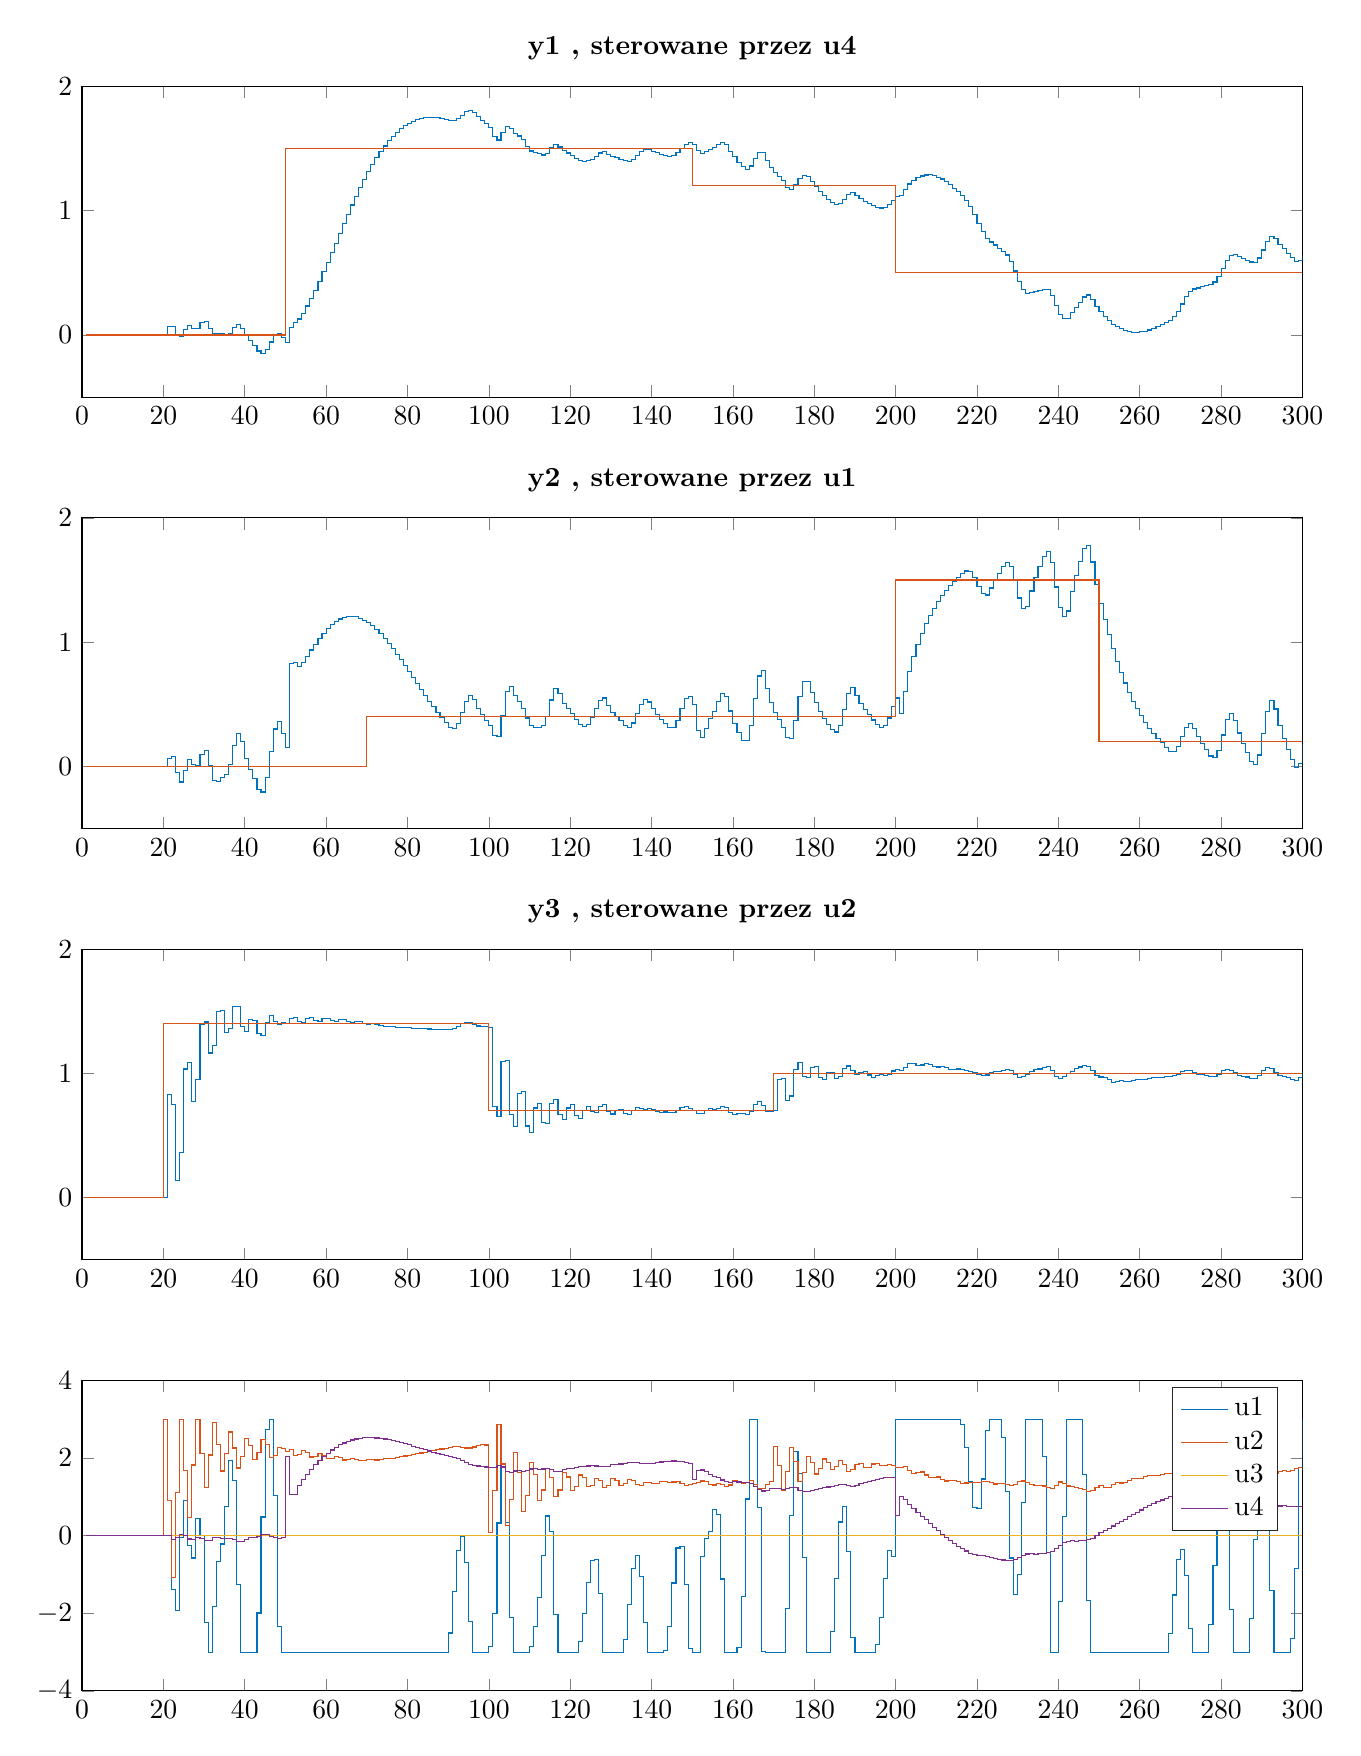
\begin{tikzpicture}

\begin{axis}[%
width=6.102in,
height=1.553in,
at={(1.024in,7.552in)},
scale only axis,
xmin=0,
xmax=300,
ymin=-0.5,
ymax=2,
axis background/.style={fill=white},
title style={font=\bfseries},
title={y1 , sterowane przez u4}
]
\addplot[const plot, color=mycolor1, forget plot] table[row sep=crcr] {%
1	0\\
2	0\\
3	0\\
4	0\\
5	0\\
6	0\\
7	0\\
8	0\\
9	0\\
10	0\\
11	0\\
12	0\\
13	0\\
14	0\\
15	0\\
16	0\\
17	0\\
18	0\\
19	0\\
20	0\\
21	0.0663597650785785\\
22	0.071588966531205\\
23	0.00204503543849707\\
24	-0.0149567001131553\\
25	0.0451621301910334\\
26	0.0764232502448876\\
27	0.0509863481737071\\
28	0.0540700821324037\\
29	0.100706978883226\\
30	0.108891766767745\\
31	0.0538783639722725\\
32	0.00969566544948017\\
33	0.00844500107202978\\
34	0.00901575567590383\\
35	-0.0019863630699275\\
36	0.0147983159246805\\
37	0.0633382485696575\\
38	0.0873795103551658\\
39	0.0507379280878118\\
40	-0.00472382290978559\\
41	-0.0431079170688042\\
42	-0.0829915532446915\\
43	-0.129418952818674\\
44	-0.150513930152023\\
45	-0.119765788810193\\
46	-0.0570036082898798\\
47	-0.00308057603403272\\
48	0.0149365245898451\\
49	-0.0188380528561138\\
50	-0.061368938324014\\
51	0.0606740268308179\\
52	0.0982868674191354\\
53	0.128800374988801\\
54	0.175220296566723\\
55	0.233396266646549\\
56	0.296150747384201\\
57	0.361231109748659\\
58	0.431564474218715\\
59	0.50738629201986\\
60	0.584620933935258\\
61	0.66136937300366\\
62	0.739386736067969\\
63	0.818791657181802\\
64	0.896812268375463\\
65	0.972107264609049\\
66	1.04582882025129\\
67	1.11809560899855\\
68	1.18709298101409\\
69	1.25194922244903\\
70	1.31349234794271\\
71	1.37189925093106\\
72	1.42605303630672\\
73	1.47545655817929\\
74	1.52076881836226\\
75	1.56223825595485\\
76	1.5992453569636\\
77	1.63157491839914\\
78	1.65979465258997\\
79	1.68421115975121\\
80	1.70454541670421\\
81	1.72077816588434\\
82	1.73341620780552\\
83	1.74279682490796\\
84	1.74885829608328\\
85	1.75170141120044\\
86	1.75177630772675\\
87	1.74941928115534\\
88	1.74469111504176\\
89	1.73775003171559\\
90	1.72898262501337\\
91	1.7267647415478\\
92	1.74032119753973\\
93	1.7680333157054\\
94	1.7962446871631\\
95	1.80767599807199\\
96	1.79025142148656\\
97	1.75906014513935\\
98	1.72970319008567\\
99	1.70128681785534\\
100	1.67243945960273\\
101	1.59598180172116\\
102	1.56923850727989\\
103	1.62708536093963\\
104	1.67742586535112\\
105	1.65904508204073\\
106	1.62014431060968\\
107	1.60168187911843\\
108	1.57098213768714\\
109	1.51753245081457\\
110	1.48085338100089\\
111	1.47109235302677\\
112	1.46169892650952\\
113	1.44846140626783\\
114	1.46280401175748\\
115	1.50751633461102\\
116	1.53568828529541\\
117	1.51333358604261\\
118	1.48137206922179\\
119	1.4649880978706\\
120	1.44745132985658\\
121	1.42213833903764\\
122	1.40212596725986\\
123	1.39646287370357\\
124	1.40167993597652\\
125	1.41438240325818\\
126	1.4375476237646\\
127	1.46439584915595\\
128	1.47325020206235\\
129	1.45251155720109\\
130	1.43524045753696\\
131	1.42554174427361\\
132	1.41585660924916\\
133	1.40380129038611\\
134	1.39962037687131\\
135	1.414329994617\\
136	1.44359224877101\\
137	1.47319543840744\\
138	1.49151111932139\\
139	1.49067798993352\\
140	1.47760375464154\\
141	1.46532093077266\\
142	1.45525778214364\\
143	1.44696799008103\\
144	1.43977532821552\\
145	1.44317490917119\\
146	1.46568359472569\\
147	1.50200389464564\\
148	1.53487241361508\\
149	1.54737705349816\\
150	1.53174403858766\\
151	1.48431606587452\\
152	1.45787950607969\\
153	1.47438280687756\\
154	1.49446461753683\\
155	1.50955331867957\\
156	1.53007160076423\\
157	1.54645974661079\\
158	1.53065440000916\\
159	1.48024599249235\\
160	1.43299411768533\\
161	1.3916084794432\\
162	1.35268196870114\\
163	1.33482067379421\\
164	1.35990714241614\\
165	1.41725533103828\\
166	1.46579880422673\\
167	1.46755161988642\\
168	1.40669578196446\\
169	1.3514692836132\\
170	1.30419950835198\\
171	1.27886393120291\\
172	1.24031467462327\\
173	1.18708474023525\\
174	1.1690912824094\\
175	1.207219796367\\
176	1.25908807614344\\
177	1.28282611399742\\
178	1.27422118792205\\
179	1.23628877705268\\
180	1.19661243051626\\
181	1.15457546373271\\
182	1.11963842966414\\
183	1.09364939269821\\
184	1.06711394129056\\
185	1.04735780524127\\
186	1.0552966027218\\
187	1.09219030255772\\
188	1.13090407965948\\
189	1.14316545667901\\
190	1.11956549459807\\
191	1.09601963441491\\
192	1.07699509561628\\
193	1.0577710343097\\
194	1.04085609924177\\
195	1.02872644087017\\
196	1.02200384211635\\
197	1.02675813417736\\
198	1.04917702076441\\
199	1.08419627020536\\
200	1.11429054186122\\
201	1.12347177274295\\
202	1.17180149474172\\
203	1.21523550464676\\
204	1.24512256692958\\
205	1.26516430512876\\
206	1.2794938494353\\
207	1.28797220183109\\
208	1.28840072604077\\
209	1.28168831850786\\
210	1.27059646587855\\
211	1.25541103544655\\
212	1.23488040461645\\
213	1.20975518602197\\
214	1.18204185406801\\
215	1.15209215510775\\
216	1.119183593482\\
217	1.08173345196801\\
218	1.03375763974468\\
219	0.971325328595297\\
220	0.899195104066027\\
221	0.830147526151137\\
222	0.777671410469336\\
223	0.748352085056901\\
224	0.723928813367032\\
225	0.698405004394665\\
226	0.674055448559362\\
227	0.643912165292073\\
228	0.592167819777517\\
229	0.515063563273117\\
230	0.429835288843451\\
231	0.362766806007066\\
232	0.333653631112196\\
233	0.343019925555142\\
234	0.352113067404777\\
235	0.359813259589204\\
236	0.369466415654389\\
237	0.364866848988361\\
238	0.320302543423007\\
239	0.238252336554022\\
240	0.167181338229765\\
241	0.129669148305035\\
242	0.133473901121782\\
243	0.178983599014095\\
244	0.223357130240415\\
245	0.264745541624045\\
246	0.305522904294985\\
247	0.321972519660824\\
248	0.284735828287027\\
249	0.230046340598273\\
250	0.185910644526793\\
251	0.149229917695879\\
252	0.115891144910142\\
253	0.0872332330824957\\
254	0.0652215307011682\\
255	0.0485573603629068\\
256	0.0353530012599587\\
257	0.0262250757089997\\
258	0.0222296512090536\\
259	0.0223423742974243\\
260	0.0251369051296305\\
261	0.0308714424761208\\
262	0.0401422919128499\\
263	0.0521731213214993\\
264	0.0659082846045754\\
265	0.0814257852547431\\
266	0.0990574719174965\\
267	0.118228156540657\\
268	0.146151506935267\\
269	0.190670174052107\\
270	0.249283860682129\\
271	0.308333107865934\\
272	0.351831393517321\\
273	0.370095661261409\\
274	0.378330593734031\\
275	0.388126077746996\\
276	0.397907441671295\\
277	0.406555110386493\\
278	0.426556949141636\\
279	0.471253461768208\\
280	0.53641496250645\\
281	0.601220466028065\\
282	0.642446210454802\\
283	0.645292739920406\\
284	0.629256107310952\\
285	0.615039448658245\\
286	0.601590882184268\\
287	0.587172613743468\\
288	0.586635159336746\\
289	0.619747372183799\\
290	0.684195820052947\\
291	0.752319599945985\\
292	0.789872617117877\\
293	0.773796727332811\\
294	0.731632734640519\\
295	0.693677684495313\\
296	0.658179623197798\\
297	0.622527757335509\\
298	0.593778263241783\\
299	0.596845384838136\\
300	0.642553554187909\\
};
\addplot[const plot, color=mycolor2, forget plot] table[row sep=crcr] {%
1	0\\
2	0\\
3	0\\
4	0\\
5	0\\
6	0\\
7	0\\
8	0\\
9	0\\
10	0\\
11	0\\
12	0\\
13	0\\
14	0\\
15	0\\
16	0\\
17	0\\
18	0\\
19	0\\
20	0\\
21	0\\
22	0\\
23	0\\
24	0\\
25	0\\
26	0\\
27	0\\
28	0\\
29	0\\
30	0\\
31	0\\
32	0\\
33	0\\
34	0\\
35	0\\
36	0\\
37	0\\
38	0\\
39	0\\
40	0\\
41	0\\
42	0\\
43	0\\
44	0\\
45	0\\
46	0\\
47	0\\
48	0\\
49	0\\
50	1.5\\
51	1.5\\
52	1.5\\
53	1.5\\
54	1.5\\
55	1.5\\
56	1.5\\
57	1.5\\
58	1.5\\
59	1.5\\
60	1.5\\
61	1.5\\
62	1.5\\
63	1.5\\
64	1.5\\
65	1.5\\
66	1.5\\
67	1.5\\
68	1.5\\
69	1.5\\
70	1.5\\
71	1.5\\
72	1.5\\
73	1.5\\
74	1.5\\
75	1.5\\
76	1.5\\
77	1.5\\
78	1.5\\
79	1.5\\
80	1.5\\
81	1.5\\
82	1.5\\
83	1.5\\
84	1.5\\
85	1.5\\
86	1.5\\
87	1.5\\
88	1.5\\
89	1.5\\
90	1.5\\
91	1.5\\
92	1.5\\
93	1.5\\
94	1.5\\
95	1.5\\
96	1.5\\
97	1.5\\
98	1.5\\
99	1.5\\
100	1.5\\
101	1.5\\
102	1.5\\
103	1.5\\
104	1.5\\
105	1.5\\
106	1.5\\
107	1.5\\
108	1.5\\
109	1.5\\
110	1.5\\
111	1.5\\
112	1.5\\
113	1.5\\
114	1.5\\
115	1.5\\
116	1.5\\
117	1.5\\
118	1.5\\
119	1.5\\
120	1.5\\
121	1.5\\
122	1.5\\
123	1.5\\
124	1.5\\
125	1.5\\
126	1.5\\
127	1.5\\
128	1.5\\
129	1.5\\
130	1.5\\
131	1.5\\
132	1.5\\
133	1.5\\
134	1.5\\
135	1.5\\
136	1.5\\
137	1.5\\
138	1.5\\
139	1.5\\
140	1.5\\
141	1.5\\
142	1.5\\
143	1.5\\
144	1.5\\
145	1.5\\
146	1.5\\
147	1.5\\
148	1.5\\
149	1.5\\
150	1.2\\
151	1.2\\
152	1.2\\
153	1.2\\
154	1.2\\
155	1.2\\
156	1.2\\
157	1.2\\
158	1.2\\
159	1.2\\
160	1.2\\
161	1.2\\
162	1.2\\
163	1.2\\
164	1.2\\
165	1.2\\
166	1.2\\
167	1.2\\
168	1.2\\
169	1.2\\
170	1.2\\
171	1.2\\
172	1.2\\
173	1.2\\
174	1.2\\
175	1.2\\
176	1.2\\
177	1.2\\
178	1.2\\
179	1.2\\
180	1.2\\
181	1.2\\
182	1.2\\
183	1.2\\
184	1.2\\
185	1.2\\
186	1.2\\
187	1.2\\
188	1.2\\
189	1.2\\
190	1.2\\
191	1.2\\
192	1.2\\
193	1.2\\
194	1.2\\
195	1.2\\
196	1.2\\
197	1.2\\
198	1.2\\
199	1.2\\
200	0.5\\
201	0.5\\
202	0.5\\
203	0.5\\
204	0.5\\
205	0.5\\
206	0.5\\
207	0.5\\
208	0.5\\
209	0.5\\
210	0.5\\
211	0.5\\
212	0.5\\
213	0.5\\
214	0.5\\
215	0.5\\
216	0.5\\
217	0.5\\
218	0.5\\
219	0.5\\
220	0.5\\
221	0.5\\
222	0.5\\
223	0.5\\
224	0.5\\
225	0.5\\
226	0.5\\
227	0.5\\
228	0.5\\
229	0.5\\
230	0.5\\
231	0.5\\
232	0.5\\
233	0.5\\
234	0.5\\
235	0.5\\
236	0.5\\
237	0.5\\
238	0.5\\
239	0.5\\
240	0.5\\
241	0.5\\
242	0.5\\
243	0.5\\
244	0.5\\
245	0.5\\
246	0.5\\
247	0.5\\
248	0.5\\
249	0.5\\
250	0.5\\
251	0.5\\
252	0.5\\
253	0.5\\
254	0.5\\
255	0.5\\
256	0.5\\
257	0.5\\
258	0.5\\
259	0.5\\
260	0.5\\
261	0.5\\
262	0.5\\
263	0.5\\
264	0.5\\
265	0.5\\
266	0.5\\
267	0.5\\
268	0.5\\
269	0.5\\
270	0.5\\
271	0.5\\
272	0.5\\
273	0.5\\
274	0.5\\
275	0.5\\
276	0.5\\
277	0.5\\
278	0.5\\
279	0.5\\
280	0.5\\
281	0.5\\
282	0.5\\
283	0.5\\
284	0.5\\
285	0.5\\
286	0.5\\
287	0.5\\
288	0.5\\
289	0.5\\
290	0.5\\
291	0.5\\
292	0.5\\
293	0.5\\
294	0.5\\
295	0.5\\
296	0.5\\
297	0.5\\
298	0.5\\
299	0.5\\
300	0.5\\
};
\end{axis}

\begin{axis}[%
width=6.102in,
height=1.553in,
at={(1.024in,5.395in)},
scale only axis,
xmin=0,
xmax=300,
ymin=-0.5,
ymax=2,
axis background/.style={fill=white},
title style={font=\bfseries},
title={y2 , sterowane przez u1}
]
\addplot[const plot, color=mycolor1, forget plot] table[row sep=crcr] {%
1	0\\
2	0\\
3	0\\
4	0\\
5	0\\
6	0\\
7	0\\
8	0\\
9	0\\
10	0\\
11	0\\
12	0\\
13	0\\
14	0\\
15	0\\
16	0\\
17	0\\
18	0\\
19	0\\
20	0\\
21	0.0612158143362928\\
22	0.0770823080206103\\
23	-0.0491831781100103\\
24	-0.12543318523983\\
25	-0.0318326277228493\\
26	0.0540615309589488\\
27	0.0185616141746837\\
28	0.00704896882583501\\
29	0.0954570771833016\\
30	0.126025681734124\\
31	0.00608274652286961\\
32	-0.112958445809666\\
33	-0.121630336738484\\
34	-0.0878517336522623\\
35	-0.0646306924541773\\
36	0.0142795900661495\\
37	0.165847769690918\\
38	0.263397483540801\\
39	0.198307802891116\\
40	0.0661357122380609\\
41	-0.0224283207296499\\
42	-0.0993977265642168\\
43	-0.18410344919029\\
44	-0.206617864197739\\
45	-0.0920453075789225\\
46	0.117396419559488\\
47	0.300686509996146\\
48	0.364145240478236\\
49	0.265005879072089\\
50	0.151847498174863\\
51	0.829411394904732\\
52	0.838887161616879\\
53	0.805434206795249\\
54	0.83660335388808\\
55	0.887180040201094\\
56	0.936944422413403\\
57	0.982518626357827\\
58	1.02728010776868\\
59	1.07142520443077\\
60	1.10976859176798\\
61	1.14007161061737\\
62	1.16525545855015\\
63	1.18638388002288\\
64	1.20062731358243\\
65	1.20690716871094\\
66	1.20755517206585\\
67	1.20366894517669\\
68	1.19368592853347\\
69	1.17714767978053\\
70	1.15587728156853\\
71	1.13089140544529\\
72	1.10139601352191\\
73	1.06729053968691\\
74	1.02999715371576\\
75	0.990406742098883\\
76	0.94817274995304\\
77	0.903376146633009\\
78	0.857107884985469\\
79	0.810103331201424\\
80	0.762247359153443\\
81	0.713681324769139\\
82	0.66521159075399\\
83	0.617402466640691\\
84	0.570230639188252\\
85	0.52382136156838\\
86	0.478734777829709\\
87	0.435364124761784\\
88	0.393695375983083\\
89	0.353797095324299\\
90	0.31602106488668\\
91	0.304611167330536\\
92	0.346246082182585\\
93	0.433972328464899\\
94	0.525583988782482\\
95	0.570329731638747\\
96	0.534834390625118\\
97	0.467080424597133\\
98	0.414523728641617\\
99	0.370716014911951\\
100	0.328706251227245\\
101	0.250320181329033\\
102	0.241691410647306\\
103	0.408340046426806\\
104	0.600526659712974\\
105	0.63993452242827\\
106	0.57190856080892\\
107	0.51864355613376\\
108	0.467089582013023\\
109	0.389004163406602\\
110	0.330917183553744\\
111	0.313517237735249\\
112	0.313212827548045\\
113	0.325979447635314\\
114	0.399508915338664\\
115	0.534135949445679\\
116	0.626605070127955\\
117	0.584764841840098\\
118	0.506174662105712\\
119	0.462948417494264\\
120	0.425026355085572\\
121	0.376158134766351\\
122	0.334204143608463\\
123	0.31985183012349\\
124	0.340275578653988\\
125	0.389898243760047\\
126	0.462197044306397\\
127	0.532776703448538\\
128	0.55031763560507\\
129	0.486816340215623\\
130	0.434168986395865\\
131	0.401135748516981\\
132	0.368381501363059\\
133	0.332355116882712\\
134	0.31609043147166\\
135	0.349394532689644\\
136	0.424735305153424\\
137	0.501142572488615\\
138	0.539730062979337\\
139	0.517795394661343\\
140	0.463140575026843\\
141	0.417737808976226\\
142	0.380191522634186\\
143	0.345352329432253\\
144	0.313691881156521\\
145	0.314256345487593\\
146	0.370158374797672\\
147	0.463417751760059\\
148	0.543701201194495\\
149	0.562899961138048\\
150	0.499985785933667\\
151	0.290109422898392\\
152	0.231195067346249\\
153	0.304001390868043\\
154	0.382084864863826\\
155	0.441019306971153\\
156	0.519073211758125\\
157	0.587084206661948\\
158	0.56348959104854\\
159	0.445816387331607\\
160	0.347072508532767\\
161	0.271289436690652\\
162	0.205254099823307\\
163	0.205494840859813\\
164	0.331166319616995\\
165	0.545044554621079\\
166	0.72718552217021\\
167	0.769436767775447\\
168	0.628496218802269\\
169	0.513222098189993\\
170	0.43343279702468\\
171	0.375498260717615\\
172	0.310559044140665\\
173	0.229213771627101\\
174	0.227174424561271\\
175	0.366368467943693\\
176	0.559318504554291\\
177	0.679809622428652\\
178	0.685339444413414\\
179	0.591100104024439\\
180	0.511509618681349\\
181	0.444059944258149\\
182	0.385832796098916\\
183	0.34025461248981\\
184	0.295984055079725\\
185	0.276618589277514\\
186	0.330402969937429\\
187	0.457140101137399\\
188	0.585282027141682\\
189	0.633666472770431\\
190	0.569872937639079\\
191	0.504365170245033\\
192	0.458845282206636\\
193	0.414776892424423\\
194	0.372917290793014\\
195	0.337831000873892\\
196	0.315947122662619\\
197	0.32830874225931\\
198	0.389046123433403\\
199	0.479356977895415\\
200	0.550078333075852\\
201	0.424817709003763\\
202	0.605394389198864\\
203	0.766895894672222\\
204	0.883981486529836\\
205	0.981927438698948\\
206	1.07010034803122\\
207	1.14886087934708\\
208	1.21613208439809\\
209	1.27376121919229\\
210	1.32598315987465\\
211	1.37368037444079\\
212	1.41542030419432\\
213	1.45224667630253\\
214	1.48691972182421\\
215	1.52000902984034\\
216	1.55049722060806\\
217	1.57254492264083\\
218	1.56596637698167\\
219	1.51909585943038\\
220	1.44776769649913\\
221	1.38903488530818\\
222	1.37957706068308\\
223	1.43576197703401\\
224	1.50083999990053\\
225	1.55584160567187\\
226	1.60959787147792\\
227	1.64168835978611\\
228	1.60621461197056\\
229	1.49356413232996\\
230	1.35526495539937\\
231	1.26810185378593\\
232	1.28798350453117\\
233	1.41132431686484\\
234	1.51785520107392\\
235	1.60561237737835\\
236	1.69224852582584\\
237	1.72981397845786\\
238	1.64351247576969\\
239	1.44400005438746\\
240	1.27718879239587\\
241	1.20730638147012\\
242	1.25065788371278\\
243	1.40488257383291\\
244	1.53803079440045\\
245	1.64740578357508\\
246	1.75135712382288\\
247	1.77936030068808\\
248	1.64490175849016\\
249	1.46125679305526\\
250	1.31368533108125\\
251	1.18568808037296\\
252	1.06330328579252\\
253	0.949392259389752\\
254	0.847376524735254\\
255	0.755439522817939\\
256	0.670655540026849\\
257	0.593399173974806\\
258	0.524784320545362\\
259	0.463200572005967\\
260	0.406406816780219\\
261	0.354417799465784\\
262	0.307842217627033\\
263	0.265522766784249\\
264	0.225884927192448\\
265	0.188882966890335\\
266	0.154913369378907\\
267	0.123212771975771\\
268	0.116485191696725\\
269	0.157686615179646\\
270	0.237576561349679\\
271	0.31569438724736\\
272	0.346799114722838\\
273	0.30497121919968\\
274	0.238546766302296\\
275	0.183862718450448\\
276	0.133864682862129\\
277	0.083464087982681\\
278	0.0691702677369236\\
279	0.130137244145697\\
280	0.252690842198037\\
281	0.374233970145666\\
282	0.426858405359897\\
283	0.370474977020817\\
284	0.26863502347937\\
285	0.185349067922005\\
286	0.112496561677029\\
287	0.0410750645271019\\
288	0.014814661330293\\
289	0.0912748259437978\\
290	0.261077735101326\\
291	0.440319169856409\\
292	0.528549882022169\\
293	0.462091939706394\\
294	0.329951964375283\\
295	0.225754074258481\\
296	0.13762066037481\\
297	0.0520867757591915\\
298	-0.0111822401539498\\
299	0.0205602839887309\\
300	0.178569789282111\\
};
\addplot[const plot, color=mycolor2, forget plot] table[row sep=crcr] {%
1	0\\
2	0\\
3	0\\
4	0\\
5	0\\
6	0\\
7	0\\
8	0\\
9	0\\
10	0\\
11	0\\
12	0\\
13	0\\
14	0\\
15	0\\
16	0\\
17	0\\
18	0\\
19	0\\
20	0\\
21	0\\
22	0\\
23	0\\
24	0\\
25	0\\
26	0\\
27	0\\
28	0\\
29	0\\
30	0\\
31	0\\
32	0\\
33	0\\
34	0\\
35	0\\
36	0\\
37	0\\
38	0\\
39	0\\
40	0\\
41	0\\
42	0\\
43	0\\
44	0\\
45	0\\
46	0\\
47	0\\
48	0\\
49	0\\
50	0\\
51	0\\
52	0\\
53	0\\
54	0\\
55	0\\
56	0\\
57	0\\
58	0\\
59	0\\
60	0\\
61	0\\
62	0\\
63	0\\
64	0\\
65	0\\
66	0\\
67	0\\
68	0\\
69	0\\
70	0.4\\
71	0.4\\
72	0.4\\
73	0.4\\
74	0.4\\
75	0.4\\
76	0.4\\
77	0.4\\
78	0.4\\
79	0.4\\
80	0.4\\
81	0.4\\
82	0.4\\
83	0.4\\
84	0.4\\
85	0.4\\
86	0.4\\
87	0.4\\
88	0.4\\
89	0.4\\
90	0.4\\
91	0.4\\
92	0.4\\
93	0.4\\
94	0.4\\
95	0.4\\
96	0.4\\
97	0.4\\
98	0.4\\
99	0.4\\
100	0.4\\
101	0.4\\
102	0.4\\
103	0.4\\
104	0.4\\
105	0.4\\
106	0.4\\
107	0.4\\
108	0.4\\
109	0.4\\
110	0.4\\
111	0.4\\
112	0.4\\
113	0.4\\
114	0.4\\
115	0.4\\
116	0.4\\
117	0.4\\
118	0.4\\
119	0.4\\
120	0.4\\
121	0.4\\
122	0.4\\
123	0.4\\
124	0.4\\
125	0.4\\
126	0.4\\
127	0.4\\
128	0.4\\
129	0.4\\
130	0.4\\
131	0.4\\
132	0.4\\
133	0.4\\
134	0.4\\
135	0.4\\
136	0.4\\
137	0.4\\
138	0.4\\
139	0.4\\
140	0.4\\
141	0.4\\
142	0.4\\
143	0.4\\
144	0.4\\
145	0.4\\
146	0.4\\
147	0.4\\
148	0.4\\
149	0.4\\
150	0.4\\
151	0.4\\
152	0.4\\
153	0.4\\
154	0.4\\
155	0.4\\
156	0.4\\
157	0.4\\
158	0.4\\
159	0.4\\
160	0.4\\
161	0.4\\
162	0.4\\
163	0.4\\
164	0.4\\
165	0.4\\
166	0.4\\
167	0.4\\
168	0.4\\
169	0.4\\
170	0.4\\
171	0.4\\
172	0.4\\
173	0.4\\
174	0.4\\
175	0.4\\
176	0.4\\
177	0.4\\
178	0.4\\
179	0.4\\
180	0.4\\
181	0.4\\
182	0.4\\
183	0.4\\
184	0.4\\
185	0.4\\
186	0.4\\
187	0.4\\
188	0.4\\
189	0.4\\
190	0.4\\
191	0.4\\
192	0.4\\
193	0.4\\
194	0.4\\
195	0.4\\
196	0.4\\
197	0.4\\
198	0.4\\
199	0.4\\
200	1.5\\
201	1.5\\
202	1.5\\
203	1.5\\
204	1.5\\
205	1.5\\
206	1.5\\
207	1.5\\
208	1.5\\
209	1.5\\
210	1.5\\
211	1.5\\
212	1.5\\
213	1.5\\
214	1.5\\
215	1.5\\
216	1.5\\
217	1.5\\
218	1.5\\
219	1.5\\
220	1.5\\
221	1.5\\
222	1.5\\
223	1.5\\
224	1.5\\
225	1.5\\
226	1.5\\
227	1.5\\
228	1.5\\
229	1.5\\
230	1.5\\
231	1.5\\
232	1.5\\
233	1.5\\
234	1.5\\
235	1.5\\
236	1.5\\
237	1.5\\
238	1.5\\
239	1.5\\
240	1.5\\
241	1.5\\
242	1.5\\
243	1.5\\
244	1.5\\
245	1.5\\
246	1.5\\
247	1.5\\
248	1.5\\
249	1.5\\
250	0.2\\
251	0.2\\
252	0.2\\
253	0.2\\
254	0.2\\
255	0.2\\
256	0.2\\
257	0.2\\
258	0.2\\
259	0.2\\
260	0.2\\
261	0.2\\
262	0.2\\
263	0.2\\
264	0.2\\
265	0.2\\
266	0.2\\
267	0.2\\
268	0.2\\
269	0.2\\
270	0.2\\
271	0.2\\
272	0.2\\
273	0.2\\
274	0.2\\
275	0.2\\
276	0.2\\
277	0.2\\
278	0.2\\
279	0.2\\
280	0.2\\
281	0.2\\
282	0.2\\
283	0.2\\
284	0.2\\
285	0.2\\
286	0.2\\
287	0.2\\
288	0.2\\
289	0.2\\
290	0.2\\
291	0.2\\
292	0.2\\
293	0.2\\
294	0.2\\
295	0.2\\
296	0.2\\
297	0.2\\
298	0.2\\
299	0.2\\
300	0.2\\
};
\end{axis}

\begin{axis}[%
width=6.102in,
height=1.553in,
at={(1.024in,3.239in)},
scale only axis,
xmin=0,
xmax=300,
ymin=-0.5,
ymax=2,
axis background/.style={fill=white},
title style={font=\bfseries},
title={y3 , sterowane przez u2}
]
\addplot[const plot, color=mycolor1, forget plot] table[row sep=crcr] {%
1	0\\
2	0\\
3	0\\
4	0\\
5	0\\
6	0\\
7	0\\
8	0\\
9	0\\
10	0\\
11	0\\
12	0\\
13	0\\
14	0\\
15	0\\
16	0\\
17	0\\
18	0\\
19	0\\
20	0\\
21	0.82628561460347\\
22	0.749053243317543\\
23	0.138689062657917\\
24	0.362386890682633\\
25	1.03447761102357\\
26	1.0877851149937\\
27	0.773695208503412\\
28	0.951464003054223\\
29	1.39397330903113\\
30	1.4127788323083\\
31	1.16363180380025\\
32	1.22492739959901\\
33	1.49685275845403\\
34	1.50797073994266\\
35	1.33089982431234\\
36	1.35905792409311\\
37	1.54128369548852\\
38	1.53992155093428\\
39	1.37461924716454\\
40	1.33500018066105\\
41	1.43051129942079\\
42	1.42814425374984\\
43	1.31957285083924\\
44	1.30619639402855\\
45	1.41058791939161\\
46	1.46334172858532\\
47	1.42037112111602\\
48	1.39474008191972\\
49	1.4095169226487\\
50	1.401797001529\\
51	1.44168787671612\\
52	1.45217840964235\\
53	1.41654274176041\\
54	1.40793556933217\\
55	1.43834676605789\\
56	1.44715107999829\\
57	1.42391452746013\\
58	1.41790337404146\\
59	1.43775788171275\\
60	1.4429883689206\\
61	1.42601248204676\\
62	1.41978667319607\\
63	1.43074263157893\\
64	1.43198711154869\\
65	1.41810763989469\\
66	1.41117272059527\\
67	1.41592628099606\\
68	1.41450069126963\\
69	1.40302444377173\\
70	1.39623983323215\\
71	1.3975821039791\\
72	1.39515232880666\\
73	1.38616342681745\\
74	1.3804338326626\\
75	1.38041371728336\\
76	1.37816340075705\\
77	1.37167227283287\\
78	1.36746577953312\\
79	1.36727578558856\\
80	1.36579986409865\\
81	1.36159078510545\\
82	1.35898025002308\\
83	1.3591858917462\\
84	1.358665534943\\
85	1.35638098545069\\
86	1.35520480025591\\
87	1.35598916503611\\
88	1.35636693079607\\
89	1.35559523314813\\
90	1.35557658178511\\
91	1.36162448704065\\
92	1.37751108370915\\
93	1.39777202512221\\
94	1.41059771380041\\
95	1.40895791317123\\
96	1.39414732839175\\
97	1.3805626003818\\
98	1.37759095751236\\
99	1.37503077185951\\
100	1.36570236452631\\
101	0.73320079110559\\
102	0.652952715622763\\
103	1.09738777833527\\
104	1.10679243286289\\
105	0.671390353189185\\
106	0.570393118442276\\
107	0.838562139587429\\
108	0.851423190122393\\
109	0.576027042737304\\
110	0.522142087408003\\
111	0.720820647150091\\
112	0.757097439012767\\
113	0.60142091382183\\
114	0.593284719637531\\
115	0.755363255937991\\
116	0.792928875280828\\
117	0.665583950081918\\
118	0.625784802169923\\
119	0.720923015126638\\
120	0.745923418610364\\
121	0.660666874902906\\
122	0.633222520700746\\
123	0.700704297312262\\
124	0.730142953483556\\
125	0.690198927101269\\
126	0.685635166214289\\
127	0.736163080972646\\
128	0.746543624467591\\
129	0.694014637793981\\
130	0.672562690842339\\
131	0.703896722081476\\
132	0.711442771710832\\
133	0.677310849414567\\
134	0.66741318345427\\
135	0.702278229072232\\
136	0.72773050482035\\
137	0.718579628495493\\
138	0.709099311291892\\
139	0.71350427967256\\
140	0.70903573209672\\
141	0.693067721746062\\
142	0.685403915913773\\
143	0.688670336687728\\
144	0.687408535126014\\
145	0.685213408901392\\
146	0.699065501543152\\
147	0.722602890082294\\
148	0.73141990567251\\
149	0.719300770738028\\
150	0.699992598491495\\
151	0.679690828284711\\
152	0.676606287894793\\
153	0.701676453317269\\
154	0.718565540485633\\
155	0.712405485366758\\
156	0.716192536283981\\
157	0.73516193684686\\
158	0.726510224469317\\
159	0.684397341170382\\
160	0.665217810157117\\
161	0.677161794950225\\
162	0.675568792424158\\
163	0.665303883346122\\
164	0.693917127218476\\
165	0.750407863531689\\
166	0.771294588912772\\
167	0.739958892075252\\
168	0.694914308245321\\
169	0.689755073969822\\
170	0.699076734374166\\
171	0.947641535158178\\
172	0.958882275022825\\
173	0.783583553933779\\
174	0.817591652545675\\
175	1.030305530331\\
176	1.08492225516893\\
177	0.97684695009211\\
178	0.963325935046198\\
179	1.04915297471838\\
180	1.05141372050152\\
181	0.96905467562184\\
182	0.953008197560424\\
183	1.0071815235128\\
184	1.00943795459425\\
185	0.961444311539811\\
186	0.970940361529271\\
187	1.03725760660339\\
188	1.05941109826353\\
189	1.01955972420765\\
190	0.989639380422082\\
191	1.00476251012816\\
192	1.01323048935648\\
193	0.986480497047595\\
194	0.967170739702736\\
195	0.979494427853283\\
196	0.990661537318269\\
197	0.985160189573719\\
198	0.991793198081967\\
199	1.01898413019436\\
200	1.03287216557587\\
201	1.02364514611933\\
202	1.04448923942669\\
203	1.07949491642526\\
204	1.08132702233925\\
205	1.06402130639733\\
206	1.06730596531086\\
207	1.08097122708026\\
208	1.07361514698163\\
209	1.05456407934462\\
210	1.05072852776011\\
211	1.05568761708839\\
212	1.04817882669893\\
213	1.03390063921815\\
214	1.03073476289235\\
215	1.03444162172551\\
216	1.03049673440041\\
217	1.02101574849268\\
218	1.01351778840149\\
219	1.00376692371879\\
220	0.988638103709545\\
221	0.979225084249684\\
222	0.986268155115177\\
223	1.0049663344397\\
224	1.01546168134295\\
225	1.01636690075263\\
226	1.02303594119422\\
227	1.03158586179667\\
228	1.02028239666267\\
229	0.989911831934678\\
230	0.968361692642123\\
231	0.972049298448164\\
232	0.992355770457586\\
233	1.01718588465741\\
234	1.02936022251956\\
235	1.03518561282458\\
236	1.04827932739753\\
237	1.05347412752053\\
238	1.02484082445256\\
239	0.976206987342164\\
240	0.958197007220109\\
241	0.976335742462937\\
242	0.997586554788003\\
243	1.01775143447494\\
244	1.03572524370647\\
245	1.05071852506737\\
246	1.06295072557727\\
247	1.05833595355615\\
248	1.01935915559284\\
249	0.97918517041072\\
250	0.970822839143539\\
251	0.969650337186019\\
252	0.949118409492761\\
253	0.929674545797697\\
254	0.933026172327966\\
255	0.941891720232776\\
256	0.937358384035376\\
257	0.93229302769051\\
258	0.941166567707269\\
259	0.952551027043302\\
260	0.953633675106938\\
261	0.952943742786293\\
262	0.960484098004015\\
263	0.968963496024625\\
264	0.969881148931168\\
265	0.968991563117043\\
266	0.973246502981673\\
267	0.978011620383366\\
268	0.982295427453832\\
269	0.9945547236808\\
270	1.01414332000677\\
271	1.02604559676738\\
272	1.02071245492834\\
273	1.00381849764596\\
274	0.992190974148395\\
275	0.989675290666508\\
276	0.983832723021331\\
277	0.972036993628726\\
278	0.971838292672276\\
279	0.993362423572407\\
280	1.02013776210512\\
281	1.03086205238621\\
282	1.02306674211596\\
283	1.00346524643002\\
284	0.985455921786467\\
285	0.977560131930393\\
286	0.970745779863672\\
287	0.958590936388222\\
288	0.957344181297893\\
289	0.983707861826586\\
290	1.02307551263826\\
291	1.0444471023967\\
292	1.03660750791892\\
293	1.0082408318714\\
294	0.984028132010736\\
295	0.977061322827809\\
296	0.969848540802538\\
297	0.952351742885111\\
298	0.943050100798158\\
299	0.964493788198466\\
300	1.00821032012264\\
};
\addplot[const plot, color=mycolor2, forget plot] table[row sep=crcr] {%
1	0\\
2	0\\
3	0\\
4	0\\
5	0\\
6	0\\
7	0\\
8	0\\
9	0\\
10	0\\
11	0\\
12	0\\
13	0\\
14	0\\
15	0\\
16	0\\
17	0\\
18	0\\
19	0\\
20	1.4\\
21	1.4\\
22	1.4\\
23	1.4\\
24	1.4\\
25	1.4\\
26	1.4\\
27	1.4\\
28	1.4\\
29	1.4\\
30	1.4\\
31	1.4\\
32	1.4\\
33	1.4\\
34	1.4\\
35	1.4\\
36	1.4\\
37	1.4\\
38	1.4\\
39	1.4\\
40	1.4\\
41	1.4\\
42	1.4\\
43	1.4\\
44	1.4\\
45	1.4\\
46	1.4\\
47	1.4\\
48	1.4\\
49	1.4\\
50	1.4\\
51	1.4\\
52	1.4\\
53	1.4\\
54	1.4\\
55	1.4\\
56	1.4\\
57	1.4\\
58	1.4\\
59	1.4\\
60	1.4\\
61	1.4\\
62	1.4\\
63	1.4\\
64	1.4\\
65	1.4\\
66	1.4\\
67	1.4\\
68	1.4\\
69	1.4\\
70	1.4\\
71	1.4\\
72	1.4\\
73	1.4\\
74	1.4\\
75	1.4\\
76	1.4\\
77	1.4\\
78	1.4\\
79	1.4\\
80	1.4\\
81	1.4\\
82	1.4\\
83	1.4\\
84	1.4\\
85	1.4\\
86	1.4\\
87	1.4\\
88	1.4\\
89	1.4\\
90	1.4\\
91	1.4\\
92	1.4\\
93	1.4\\
94	1.4\\
95	1.4\\
96	1.4\\
97	1.4\\
98	1.4\\
99	1.4\\
100	0.7\\
101	0.7\\
102	0.7\\
103	0.7\\
104	0.7\\
105	0.7\\
106	0.7\\
107	0.7\\
108	0.7\\
109	0.7\\
110	0.7\\
111	0.7\\
112	0.7\\
113	0.7\\
114	0.7\\
115	0.7\\
116	0.7\\
117	0.7\\
118	0.7\\
119	0.7\\
120	0.7\\
121	0.7\\
122	0.7\\
123	0.7\\
124	0.7\\
125	0.7\\
126	0.7\\
127	0.7\\
128	0.7\\
129	0.7\\
130	0.7\\
131	0.7\\
132	0.7\\
133	0.7\\
134	0.7\\
135	0.7\\
136	0.7\\
137	0.7\\
138	0.7\\
139	0.7\\
140	0.7\\
141	0.7\\
142	0.7\\
143	0.7\\
144	0.7\\
145	0.7\\
146	0.7\\
147	0.7\\
148	0.7\\
149	0.7\\
150	0.7\\
151	0.7\\
152	0.7\\
153	0.7\\
154	0.7\\
155	0.7\\
156	0.7\\
157	0.7\\
158	0.7\\
159	0.7\\
160	0.7\\
161	0.7\\
162	0.7\\
163	0.7\\
164	0.7\\
165	0.7\\
166	0.7\\
167	0.7\\
168	0.7\\
169	0.7\\
170	1\\
171	1\\
172	1\\
173	1\\
174	1\\
175	1\\
176	1\\
177	1\\
178	1\\
179	1\\
180	1\\
181	1\\
182	1\\
183	1\\
184	1\\
185	1\\
186	1\\
187	1\\
188	1\\
189	1\\
190	1\\
191	1\\
192	1\\
193	1\\
194	1\\
195	1\\
196	1\\
197	1\\
198	1\\
199	1\\
200	1\\
201	1\\
202	1\\
203	1\\
204	1\\
205	1\\
206	1\\
207	1\\
208	1\\
209	1\\
210	1\\
211	1\\
212	1\\
213	1\\
214	1\\
215	1\\
216	1\\
217	1\\
218	1\\
219	1\\
220	1\\
221	1\\
222	1\\
223	1\\
224	1\\
225	1\\
226	1\\
227	1\\
228	1\\
229	1\\
230	1\\
231	1\\
232	1\\
233	1\\
234	1\\
235	1\\
236	1\\
237	1\\
238	1\\
239	1\\
240	1\\
241	1\\
242	1\\
243	1\\
244	1\\
245	1\\
246	1\\
247	1\\
248	1\\
249	1\\
250	1\\
251	1\\
252	1\\
253	1\\
254	1\\
255	1\\
256	1\\
257	1\\
258	1\\
259	1\\
260	1\\
261	1\\
262	1\\
263	1\\
264	1\\
265	1\\
266	1\\
267	1\\
268	1\\
269	1\\
270	1\\
271	1\\
272	1\\
273	1\\
274	1\\
275	1\\
276	1\\
277	1\\
278	1\\
279	1\\
280	1\\
281	1\\
282	1\\
283	1\\
284	1\\
285	1\\
286	1\\
287	1\\
288	1\\
289	1\\
290	1\\
291	1\\
292	1\\
293	1\\
294	1\\
295	1\\
296	1\\
297	1\\
298	1\\
299	1\\
300	1\\
};
\end{axis}

\begin{axis}[%
width=6.102in,
height=1.553in,
at={(1.024in,1.083in)},
scale only axis,
xmin=0,
xmax=300,
ymin=-4,
ymax=4,
axis background/.style={fill=white},
legend style={legend cell align=left, align=left, draw=white!15!black}
]
\addplot[const plot, color=mycolor1] table[row sep=crcr] {%
1	0\\
2	0\\
3	0\\
4	0\\
5	0\\
6	0\\
7	0\\
8	0\\
9	0\\
10	0\\
11	0\\
12	0\\
13	0\\
14	0\\
15	0\\
16	0\\
17	0\\
18	0\\
19	0\\
20	0\\
21	0\\
22	-1.37735582256659\\
23	-1.91799937347261\\
24	-0.0428626316309912\\
25	0.895324366872669\\
26	-0.244190484219792\\
27	-0.576112948513736\\
28	0.442442118929574\\
29	-0.00294657475276733\\
30	-2.23601528936947\\
31	-3\\
32	-1.82484592914877\\
33	-0.676975522044811\\
34	-0.215975596991852\\
35	0.74439819349961\\
36	1.94504400836129\\
37	1.41767553284362\\
38	-1.259878969462\\
39	-3\\
40	-3\\
41	-3\\
42	-3\\
43	-1.99453195339003\\
44	0.478679834145064\\
45	2.73033723815414\\
46	2.98154969710747\\
47	1.02466112960285\\
48	-2.34701147295334\\
49	-3\\
50	-3\\
51	-3\\
52	-3\\
53	-3\\
54	-3\\
55	-3\\
56	-3\\
57	-3\\
58	-3\\
59	-3\\
60	-3\\
61	-3\\
62	-3\\
63	-3\\
64	-3\\
65	-3\\
66	-3\\
67	-3\\
68	-3\\
69	-3\\
70	-3\\
71	-3\\
72	-3\\
73	-3\\
74	-3\\
75	-3\\
76	-3\\
77	-3\\
78	-3\\
79	-3\\
80	-3\\
81	-3\\
82	-3\\
83	-3\\
84	-3\\
85	-3\\
86	-3\\
87	-3\\
88	-3\\
89	-3\\
90	-2.50774431026801\\
91	-1.44351942319149\\
92	-0.380425066729853\\
93	-0.0232969315327343\\
94	-0.691209727398984\\
95	-2.20934205613033\\
96	-3\\
97	-3\\
98	-3\\
99	-3\\
100	-2.86286272217295\\
101	-2.00407582770232\\
102	0.324899812382291\\
103	1.82361159400713\\
104	0.345100881078043\\
105	-2.10441498490881\\
106	-3\\
107	-3\\
108	-3\\
109	-3\\
110	-2.86806950099972\\
111	-2.3331999286865\\
112	-1.60250265931081\\
113	-0.507211345949407\\
114	0.503694366619917\\
115	0.11278906981206\\
116	-2.02659931523554\\
117	-3\\
118	-3\\
119	-3\\
120	-3\\
121	-3\\
122	-2.7309251180054\\
123	-2.01575098227884\\
124	-1.20933397688855\\
125	-0.638873532496785\\
126	-0.614432194826939\\
127	-1.49415688224782\\
128	-3\\
129	-3\\
130	-3\\
131	-3\\
132	-3\\
133	-2.67646452133807\\
134	-1.78464435682321\\
135	-0.836332302079377\\
136	-0.522207276491536\\
137	-1.05864343265544\\
138	-2.24474725543324\\
139	-3\\
140	-3\\
141	-3\\
142	-3\\
143	-2.96610888455489\\
144	-2.33565531312867\\
145	-1.2216504868317\\
146	-0.319654530937401\\
147	-0.284521800755229\\
148	-1.26440905265305\\
149	-2.90294041778012\\
150	-3\\
151	-3\\
152	-0.5325387231639\\
153	-0.0771234231398576\\
154	0.109836020800317\\
155	0.666612875136099\\
156	0.546316642713224\\
157	-1.11797251427301\\
158	-3\\
159	-3\\
160	-3\\
161	-2.87758698160341\\
162	-1.5634820387334\\
163	0.943574628316709\\
164	3\\
165	3\\
166	0.728302663239375\\
167	-2.97899860588325\\
168	-3\\
169	-3\\
170	-3\\
171	-3\\
172	-3\\
173	-1.86655597346764\\
174	0.526056397054179\\
175	2.15759186146607\\
176	1.59363735215255\\
177	-0.572936970152246\\
178	-3\\
179	-3\\
180	-3\\
181	-3\\
182	-3\\
183	-3\\
184	-2.46070858818965\\
185	-1.11537843711915\\
186	0.349337028313697\\
187	0.757524034676358\\
188	-0.404693398465413\\
189	-2.62414267622312\\
190	-3\\
191	-3\\
192	-3\\
193	-3\\
194	-3\\
195	-2.8086330270462\\
196	-2.11526608533807\\
197	-1.11137931772228\\
198	-0.391329137122376\\
199	-0.534211912268834\\
200	3\\
201	3\\
202	3\\
203	3\\
204	3\\
205	3\\
206	3\\
207	3\\
208	3\\
209	3\\
210	3\\
211	3\\
212	3\\
213	3\\
214	3\\
215	3\\
216	2.86777128853404\\
217	2.27872324484885\\
218	1.39104992920321\\
219	0.715465791315095\\
220	0.701614233584183\\
221	1.45761379746611\\
222	2.70664864660052\\
223	3\\
224	3\\
225	3\\
226	2.53080014603514\\
227	1.14367934957713\\
228	-0.577249519853441\\
229	-1.51932973109687\\
230	-1.00359809252839\\
231	0.852865647773315\\
232	3\\
233	3\\
234	3\\
235	3\\
236	2.03600612755053\\
237	-0.444406757540036\\
238	-3\\
239	-3\\
240	-1.69927568770324\\
241	0.499827834708798\\
242	3\\
243	3\\
244	3\\
245	3\\
246	1.56637947437469\\
247	-1.67111256473157\\
248	-3\\
249	-3\\
250	-3\\
251	-3\\
252	-3\\
253	-3\\
254	-3\\
255	-3\\
256	-3\\
257	-3\\
258	-3\\
259	-3\\
260	-3\\
261	-3\\
262	-3\\
263	-3\\
264	-3\\
265	-3\\
266	-3\\
267	-2.51295208297324\\
268	-1.53102435222344\\
269	-0.60825254441909\\
270	-0.363293411584248\\
271	-1.03169934630962\\
272	-2.39431949521224\\
273	-3\\
274	-3\\
275	-3\\
276	-3\\
277	-2.28919355024173\\
278	-0.763126835445909\\
279	0.701715661790042\\
280	1.12087883358969\\
281	0.142967932131879\\
282	-1.91147190303225\\
283	-3\\
284	-3\\
285	-3\\
286	-3\\
287	-2.14048609500649\\
288	-0.0951809092282803\\
289	2.02249422899427\\
290	2.76479576687431\\
291	1.49262989703502\\
292	-1.4188335015839\\
293	-3\\
294	-3\\
295	-3\\
296	-3\\
297	-2.65368398289625\\
298	-0.85108245127103\\
299	1.76476215499935\\
300	3\\
};
\addlegendentry{u1}

\addplot[const plot, color=mycolor2] table[row sep=crcr] {%
1	0\\
2	0\\
3	0\\
4	0\\
5	0\\
6	0\\
7	0\\
8	0\\
9	0\\
10	0\\
11	0\\
12	0\\
13	0\\
14	0\\
15	0\\
16	0\\
17	0\\
18	0\\
19	0\\
20	3\\
21	0.9\\
22	-1.08542824746128\\
23	1.10500538112319\\
24	3\\
25	1.68290916627146\\
26	0.464816535871529\\
27	1.8185097831387\\
28	3\\
29	2.10722400047758\\
30	1.24887434362716\\
31	2.07578835041457\\
32	2.91673782346596\\
33	2.33741717820373\\
34	1.66378725372297\\
35	2.1230781523679\\
36	2.6668092211724\\
37	2.25570365346808\\
38	1.74025713394799\\
39	2.03849379879582\\
40	2.50304122147188\\
41	2.31388895648644\\
42	1.9567395971798\\
43	2.14019908341947\\
44	2.4742499246621\\
45	2.340794178056\\
46	2.02167060999043\\
47	2.05370982114117\\
48	2.26720104951115\\
49	2.25437515140255\\
50	2.15771829968088\\
51	2.20760326345352\\
52	2.06161957609149\\
53	2.08646315609741\\
54	2.19717093774499\\
55	2.14560154149269\\
56	2.02558302261154\\
57	2.03861801272774\\
58	2.10816989635842\\
59	2.0692757761627\\
60	1.98377463237295\\
61	1.98760562343362\\
62	2.03174404572902\\
63	2.00501990972268\\
64	1.94706809067901\\
65	1.94956413175353\\
66	1.98116781879419\\
67	1.96689354326198\\
68	1.93198827306292\\
69	1.93816541997738\\
70	1.96536169925787\\
71	1.96294696662986\\
72	1.94689544900703\\
73	1.9586857078218\\
74	1.98546392453853\\
75	1.99302558815464\\
76	1.99141485849618\\
77	2.00848129780652\\
78	2.03599513012895\\
79	2.05084784108835\\
80	2.05931944504211\\
81	2.08009830920092\\
82	2.10792604089966\\
83	2.12719672937827\\
84	2.14181719860182\\
85	2.16432669578537\\
86	2.19137800055747\\
87	2.21244101073054\\
88	2.22993705467738\\
89	2.25228346299986\\
90	2.27736354647755\\
91	2.2980831515374\\
92	2.30060186583831\\
93	2.28025399365645\\
94	2.25742358554641\\
95	2.25737596760728\\
96	2.28305784010831\\
97	2.32343368279764\\
98	2.34088921507517\\
99	2.33309629819003\\
100	0.0716781370667148\\
101	1.15935970366419\\
102	2.86348182035196\\
103	1.84268452327691\\
104	0.261298060684216\\
105	0.920909169726845\\
106	2.15137902129018\\
107	1.62312069827563\\
108	0.614380350838925\\
109	1.03963890909689\\
110	1.88468689410715\\
111	1.57100718278855\\
112	0.906460909264163\\
113	1.1755081316196\\
114	1.72546170270911\\
115	1.48984082651529\\
116	1.00017083535143\\
117	1.17455801711914\\
118	1.61709582506086\\
119	1.50896123033606\\
120	1.15727134131779\\
121	1.25583494834579\\
122	1.5599578130573\\
123	1.49830543934795\\
124	1.25748969660583\\
125	1.29642546861602\\
126	1.47004938995927\\
127	1.40989409652674\\
128	1.24373326868098\\
129	1.2929707913528\\
130	1.46117927279813\\
131	1.42883280814675\\
132	1.2978119672951\\
133	1.33400700743723\\
134	1.45430646830339\\
135	1.42955461337454\\
136	1.31274129146844\\
137	1.29861237198686\\
138	1.36539201912871\\
139	1.36861148314295\\
140	1.33078504585263\\
141	1.34736562239916\\
142	1.38580669483877\\
143	1.38224418221935\\
144	1.36359874508254\\
145	1.37989727336215\\
146	1.39080356290574\\
147	1.34878730492008\\
148	1.30046222667981\\
149	1.30758025804875\\
150	1.34889152492999\\
151	1.37775442949325\\
152	1.40512253892648\\
153	1.38469834063779\\
154	1.30874807828751\\
155	1.30316064917664\\
156	1.3476762324069\\
157	1.3168454640048\\
158	1.2546727458679\\
159	1.30314864379724\\
160	1.40945697752903\\
161	1.39536601613908\\
162	1.33558009845639\\
163	1.37606442877722\\
164	1.41845498201662\\
165	1.32228017960233\\
166	1.19895321071986\\
167	1.21884889409193\\
168	1.32681606511964\\
169	1.39056012285425\\
170	2.29478131246711\\
171	1.80928991061708\\
172	1.17055926169064\\
173	1.65733569111948\\
174	2.27009687687675\\
175	1.91718133724311\\
176	1.38508160539176\\
177	1.61785224007362\\
178	2.03586930366471\\
179	1.87523851736422\\
180	1.58759564081471\\
181	1.72732580900468\\
182	1.97380733617915\\
183	1.87671296230847\\
184	1.69205259806022\\
185	1.78947508719385\\
186	1.94524831198655\\
187	1.83767670764202\\
188	1.65566758036542\\
189	1.6976744193165\\
190	1.84179281918664\\
191	1.84955132627414\\
192	1.7457407769472\\
193	1.74608484880326\\
194	1.84334303758552\\
195	1.85935951581475\\
196	1.79710264478439\\
197	1.79570970139764\\
198	1.84059253183826\\
199	1.81545246391049\\
200	1.74445135252073\\
201	1.74420503665844\\
202	1.78553283786725\\
203	1.68751292264562\\
204	1.59318803930163\\
205	1.61749759086568\\
206	1.63674186833525\\
207	1.55944464178378\\
208	1.48794887620489\\
209	1.49870104652408\\
210	1.50909728265629\\
211	1.45617865035963\\
212	1.40702624299362\\
213	1.41350418187175\\
214	1.4208012970559\\
215	1.38558370054411\\
216	1.35183727523857\\
217	1.35485106584869\\
218	1.36252612819844\\
219	1.35742465243297\\
220	1.36736014826864\\
221	1.3951436220739\\
222	1.40115924344517\\
223	1.36983068208776\\
224	1.33001366345644\\
225	1.33081697745011\\
226	1.34113486750364\\
227	1.31308747451152\\
228	1.28712034283964\\
229	1.32516351483171\\
230	1.39111972159833\\
231	1.40546062887582\\
232	1.36619478510002\\
233	1.3215493134574\\
234	1.28528650109801\\
235	1.28678718911698\\
236	1.27752323509019\\
237	1.22902663692584\\
238	1.21419130197322\\
239	1.29090207342987\\
240	1.37927502567643\\
241	1.35243629318124\\
242	1.27836693978788\\
243	1.2574113989856\\
244	1.23558388725917\\
245	1.20862304939314\\
246	1.17797988158\\
247	1.14285253011097\\
248	1.15083957741077\\
249	1.2391166499712\\
250	1.28204892809006\\
251	1.2392859491388\\
252	1.2409604983946\\
253	1.32051909088965\\
254	1.36808858776571\\
255	1.35347080125335\\
256	1.36484793745928\\
257	1.42636651579406\\
258	1.46508305950239\\
259	1.45996682791293\\
260	1.47013113125071\\
261	1.51310593019431\\
262	1.54069666881021\\
263	1.53833877831817\\
264	1.54561939618463\\
265	1.57511407226727\\
266	1.59489995751068\\
267	1.59479644976386\\
268	1.60119644644678\\
269	1.60779849807947\\
270	1.58537568575584\\
271	1.54895397830997\\
272	1.54237711148654\\
273	1.57049157760097\\
274	1.60437442762645\\
275	1.60646671560578\\
276	1.59529215285259\\
277	1.61441148540239\\
278	1.64914610912734\\
279	1.64018193163623\\
280	1.58391195796176\\
281	1.54325915774449\\
282	1.55188701034385\\
283	1.58323932309121\\
284	1.61982019247204\\
285	1.6374148829767\\
286	1.6343295898286\\
287	1.6519045883681\\
288	1.69240623559803\\
289	1.69285303449659\\
290	1.62600547194873\\
291	1.5589340369549\\
292	1.55667391554419\\
293	1.60267222591549\\
294	1.66088098015491\\
295	1.67871848667133\\
296	1.66092115078915\\
297	1.68189841259152\\
298	1.73941317137135\\
299	1.75847404087653\\
300	1.69865372225255\\
};
\addlegendentry{u2}

\addplot[const plot, color=mycolor3] table[row sep=crcr] {%
1	0\\
2	0\\
3	0\\
4	0\\
5	0\\
6	0\\
7	0\\
8	0\\
9	0\\
10	0\\
11	0\\
12	0\\
13	0\\
14	0\\
15	0\\
16	0\\
17	0\\
18	0\\
19	0\\
20	0\\
21	0\\
22	0\\
23	0\\
24	0\\
25	0\\
26	0\\
27	0\\
28	0\\
29	0\\
30	0\\
31	0\\
32	0\\
33	0\\
34	0\\
35	0\\
36	0\\
37	0\\
38	0\\
39	0\\
40	0\\
41	0\\
42	0\\
43	0\\
44	0\\
45	0\\
46	0\\
47	0\\
48	0\\
49	0\\
50	0\\
51	0\\
52	0\\
53	0\\
54	0\\
55	0\\
56	0\\
57	0\\
58	0\\
59	0\\
60	0\\
61	0\\
62	0\\
63	0\\
64	0\\
65	0\\
66	0\\
67	0\\
68	0\\
69	0\\
70	0\\
71	0\\
72	0\\
73	0\\
74	0\\
75	0\\
76	0\\
77	0\\
78	0\\
79	0\\
80	0\\
81	0\\
82	0\\
83	0\\
84	0\\
85	0\\
86	0\\
87	0\\
88	0\\
89	0\\
90	0\\
91	0\\
92	0\\
93	0\\
94	0\\
95	0\\
96	0\\
97	0\\
98	0\\
99	0\\
100	0\\
101	0\\
102	0\\
103	0\\
104	0\\
105	0\\
106	0\\
107	0\\
108	0\\
109	0\\
110	0\\
111	0\\
112	0\\
113	0\\
114	0\\
115	0\\
116	0\\
117	0\\
118	0\\
119	0\\
120	0\\
121	0\\
122	0\\
123	0\\
124	0\\
125	0\\
126	0\\
127	0\\
128	0\\
129	0\\
130	0\\
131	0\\
132	0\\
133	0\\
134	0\\
135	0\\
136	0\\
137	0\\
138	0\\
139	0\\
140	0\\
141	0\\
142	0\\
143	0\\
144	0\\
145	0\\
146	0\\
147	0\\
148	0\\
149	0\\
150	0\\
151	0\\
152	0\\
153	0\\
154	0\\
155	0\\
156	0\\
157	0\\
158	0\\
159	0\\
160	0\\
161	0\\
162	0\\
163	0\\
164	0\\
165	0\\
166	0\\
167	0\\
168	0\\
169	0\\
170	0\\
171	0\\
172	0\\
173	0\\
174	0\\
175	0\\
176	0\\
177	0\\
178	0\\
179	0\\
180	0\\
181	0\\
182	0\\
183	0\\
184	0\\
185	0\\
186	0\\
187	0\\
188	0\\
189	0\\
190	0\\
191	0\\
192	0\\
193	0\\
194	0\\
195	0\\
196	0\\
197	0\\
198	0\\
199	0\\
200	0\\
201	0\\
202	0\\
203	0\\
204	0\\
205	0\\
206	0\\
207	0\\
208	0\\
209	0\\
210	0\\
211	0\\
212	0\\
213	0\\
214	0\\
215	0\\
216	0\\
217	0\\
218	0\\
219	0\\
220	0\\
221	0\\
222	0\\
223	0\\
224	0\\
225	0\\
226	0\\
227	0\\
228	0\\
229	0\\
230	0\\
231	0\\
232	0\\
233	0\\
234	0\\
235	0\\
236	0\\
237	0\\
238	0\\
239	0\\
240	0\\
241	0\\
242	0\\
243	0\\
244	0\\
245	0\\
246	0\\
247	0\\
248	0\\
249	0\\
250	0\\
251	0\\
252	0\\
253	0\\
254	0\\
255	0\\
256	0\\
257	0\\
258	0\\
259	0\\
260	0\\
261	0\\
262	0\\
263	0\\
264	0\\
265	0\\
266	0\\
267	0\\
268	0\\
269	0\\
270	0\\
271	0\\
272	0\\
273	0\\
274	0\\
275	0\\
276	0\\
277	0\\
278	0\\
279	0\\
280	0\\
281	0\\
282	0\\
283	0\\
284	0\\
285	0\\
286	0\\
287	0\\
288	0\\
289	0\\
290	0\\
291	0\\
292	0\\
293	0\\
294	0\\
295	0\\
296	0\\
297	0\\
298	0\\
299	0\\
300	0\\
};
\addlegendentry{u3}

\addplot[const plot, color=mycolor4] table[row sep=crcr] {%
1	0\\
2	0\\
3	0\\
4	0\\
5	0\\
6	0\\
7	0\\
8	0\\
9	0\\
10	0\\
11	0\\
12	0\\
13	0\\
14	0\\
15	0\\
16	0\\
17	0\\
18	0\\
19	0\\
20	0\\
21	0\\
22	-0.0904151799195633\\
23	-0.0527471254707263\\
24	0.0372412209887888\\
25	0.00451531137393671\\
26	-0.0891283958426979\\
27	-0.0892718739466025\\
28	-0.0391581051121466\\
29	-0.0700825078095285\\
30	-0.137917052732118\\
31	-0.124347681184519\\
32	-0.0564555604140413\\
33	-0.0470021514096489\\
34	-0.0818562381947916\\
35	-0.084690047978534\\
36	-0.0703700269637275\\
37	-0.101792551706805\\
38	-0.156350256230485\\
39	-0.158191810368465\\
40	-0.0999570838951849\\
41	-0.060045954985818\\
42	-0.0515265496285098\\
43	-0.0225038810324779\\
44	0.0192204861019504\\
45	0.0269978421617857\\
46	-0.0129582410141336\\
47	-0.0589024752983218\\
48	-0.0750374112944282\\
49	-0.0560622130855299\\
50	2.04625226360996\\
51	1.06703568971022\\
52	1.06189855860295\\
53	1.28820118207138\\
54	1.45193094205097\\
55	1.58449455808318\\
56	1.70796319904092\\
57	1.82732646176891\\
58	1.93933920921443\\
59	2.03792040129696\\
60	2.12443430684161\\
61	2.20393627497031\\
62	2.27557662353002\\
63	2.33550554598417\\
64	2.38480688940952\\
65	2.4271787864015\\
66	2.46240430944123\\
67	2.48818127878942\\
68	2.50546642110365\\
69	2.51700898160547\\
70	2.52295362763604\\
71	2.52199245949273\\
72	2.5149610110732\\
73	2.50391459452316\\
74	2.48916869473398\\
75	2.47002148796033\\
76	2.44717308509152\\
77	2.42214667804681\\
78	2.39529766177743\\
79	2.36626505829096\\
80	2.3355990230627\\
81	2.30440040872432\\
82	2.27298251644077\\
83	2.24115211293172\\
84	2.2093044296909\\
85	2.17820056578299\\
86	2.1480687113657\\
87	2.11877848054228\\
88	2.09057780800103\\
89	2.06395690292923\\
90	2.03904520669006\\
91	2.01571917769645\\
92	1.98310429042984\\
93	1.93451371967491\\
94	1.87756097377525\\
95	1.82778851023351\\
96	1.79775186039091\\
97	1.79217839495667\\
98	1.78445542002558\\
99	1.76711873206603\\
100	1.7536375764262\\
101	1.74504815202921\\
102	1.80458889184041\\
103	1.76786277899625\\
104	1.65899699192185\\
105	1.62079986747153\\
106	1.66393785509223\\
107	1.68235489426365\\
108	1.66137130119942\\
109	1.67571951881675\\
110	1.71511215682469\\
111	1.72013608359596\\
112	1.70648555573464\\
113	1.71508873285676\\
114	1.73039774715856\\
115	1.70670825520208\\
116	1.66191129823618\\
117	1.65835733188514\\
118	1.70689213450268\\
119	1.73088924351347\\
120	1.72997168237009\\
121	1.74513483947442\\
122	1.77216295882194\\
123	1.7889121303343\\
124	1.79285245197504\\
125	1.79415587057016\\
126	1.7933124167202\\
127	1.78261397719827\\
128	1.7723719935371\\
129	1.78623703687072\\
130	1.82492064756151\\
131	1.83779766031475\\
132	1.84529022021264\\
133	1.86003452803857\\
134	1.87922971581377\\
135	1.88730679408898\\
136	1.87646766198973\\
137	1.85907428557431\\
138	1.8492007119215\\
139	1.85127871858446\\
140	1.86812751219143\\
141	1.88643990552476\\
142	1.89551539548233\\
143	1.90373506004768\\
144	1.91257216006183\\
145	1.92236932944336\\
146	1.91951135487191\\
147	1.89866607192205\\
148	1.871476162384\\
149	1.85549855839339\\
150	1.45164675002636\\
151	1.67952831306112\\
152	1.6901745091309\\
153	1.65271243544655\\
154	1.57684250201361\\
155	1.52838582476896\\
156	1.48708484079729\\
157	1.43250547753619\\
158	1.38533230439245\\
159	1.37667013748807\\
160	1.39137551544728\\
161	1.38039871979685\\
162	1.36986088734546\\
163	1.36583868770742\\
164	1.33994824733682\\
165	1.27462631368962\\
166	1.19657018878749\\
167	1.14915134108614\\
168	1.15237305777224\\
169	1.20324743698285\\
170	1.20397189790332\\
171	1.20526210756408\\
172	1.18894107267671\\
173	1.21133798164685\\
174	1.24798502765891\\
175	1.2315315739068\\
176	1.16905029707772\\
177	1.12798010250253\\
178	1.12974564022969\\
179	1.1501070180409\\
180	1.18562833849987\\
181	1.20480533482865\\
182	1.23076307102758\\
183	1.25041327355257\\
184	1.26791890545578\\
185	1.29657605433867\\
186	1.3188761859184\\
187	1.31133493985658\\
188	1.28550623647435\\
189	1.27574988722221\\
190	1.29865177275708\\
191	1.34772014062311\\
192	1.37097571863315\\
193	1.3910575102979\\
194	1.41740627583716\\
195	1.44285224653325\\
196	1.46573994560499\\
197	1.48660495460101\\
198	1.49699867240029\\
199	1.49191160630207\\
200	0.527235860612863\\
201	1.00122328125885\\
202	0.936002953774532\\
203	0.799564720663716\\
204	0.695074472924402\\
205	0.599696120407238\\
206	0.503158581070922\\
207	0.404022429371507\\
208	0.306497578498062\\
209	0.21419987095012\\
210	0.125138254826364\\
211	0.0371699381939848\\
212	-0.0473379531806806\\
213	-0.125939692451098\\
214	-0.199991137357241\\
215	-0.271051295698305\\
216	-0.337670728186628\\
217	-0.398304091528214\\
218	-0.45100307220125\\
219	-0.488312822754159\\
220	-0.508349153559875\\
221	-0.518933237632662\\
222	-0.532459480355294\\
223	-0.557467275839644\\
224	-0.594209513819309\\
225	-0.615432277103924\\
226	-0.628185806401846\\
227	-0.640229209303474\\
228	-0.640395561589955\\
229	-0.611997538101713\\
230	-0.559859442498303\\
231	-0.507302269200542\\
232	-0.475333491985131\\
233	-0.472167428210862\\
234	-0.487426248194297\\
235	-0.47270010910446\\
236	-0.457431240901632\\
237	-0.446900169741555\\
238	-0.416594037263742\\
239	-0.342663180387314\\
240	-0.244059035908482\\
241	-0.180146508256122\\
242	-0.144290615421805\\
243	-0.133192986612536\\
244	-0.146340385377637\\
245	-0.130264513236409\\
246	-0.116577040045601\\
247	-0.109618660280858\\
248	-0.0750997341169352\\
249	0.0110483852149316\\
250	0.082681480555942\\
251	0.132808983727547\\
252	0.186739086611634\\
253	0.246664843355485\\
254	0.307053836878295\\
255	0.365714297775425\\
256	0.425157176618598\\
257	0.486247109580393\\
258	0.546201295703721\\
259	0.603564586680505\\
260	0.659935955471512\\
261	0.715925788896149\\
262	0.769705993286117\\
263	0.820303160496251\\
264	0.868810048487243\\
265	0.915698911875784\\
266	0.95980591229082\\
267	1.00051851657611\\
268	1.03862162411757\\
269	1.06363408733586\\
270	1.06954714533794\\
271	1.0639671592415\\
272	1.06174302667232\\
273	1.0736743717361\\
274	1.10210901126623\\
275	1.12173837230987\\
276	1.13018864710355\\
277	1.13868216624869\\
278	1.14748637855476\\
279	1.13883261942473\\
280	1.10311547333243\\
281	1.05368345595681\\
282	1.0129632876859\\
283	0.995985055468251\\
284	1.0072814783059\\
285	1.01324702131872\\
286	1.0036308992316\\
287	0.996201313047947\\
288	0.992388490346322\\
289	0.970689580504907\\
290	0.914314832058326\\
291	0.83802517059128\\
292	0.773740801275715\\
293	0.745533889300195\\
294	0.761245625730126\\
295	0.771608763028721\\
296	0.760637232867664\\
297	0.75442959070745\\
298	0.754834356007081\\
299	0.750168079353014\\
300	0.71126724799778\\
};
\addlegendentry{u4}

\end{axis}
\end{tikzpicture}%
    \caption{gre}
\end{figure}

\begin{figure}[H]
    \centering
    % This file was created by matlab2tikz.
%
%The latest updates can be retrieved from
%  http://www.mathworks.com/matlabcentral/fileexchange/22022-matlab2tikz-matlab2tikz
%where you can also make suggestions and rate matlab2tikz.
%
\definecolor{mycolor1}{rgb}{0.00000,0.44700,0.74100}%
\definecolor{mycolor2}{rgb}{0.85000,0.32500,0.09800}%
\definecolor{mycolor3}{rgb}{0.92900,0.69400,0.12500}%
\definecolor{mycolor4}{rgb}{0.49400,0.18400,0.55600}%
%
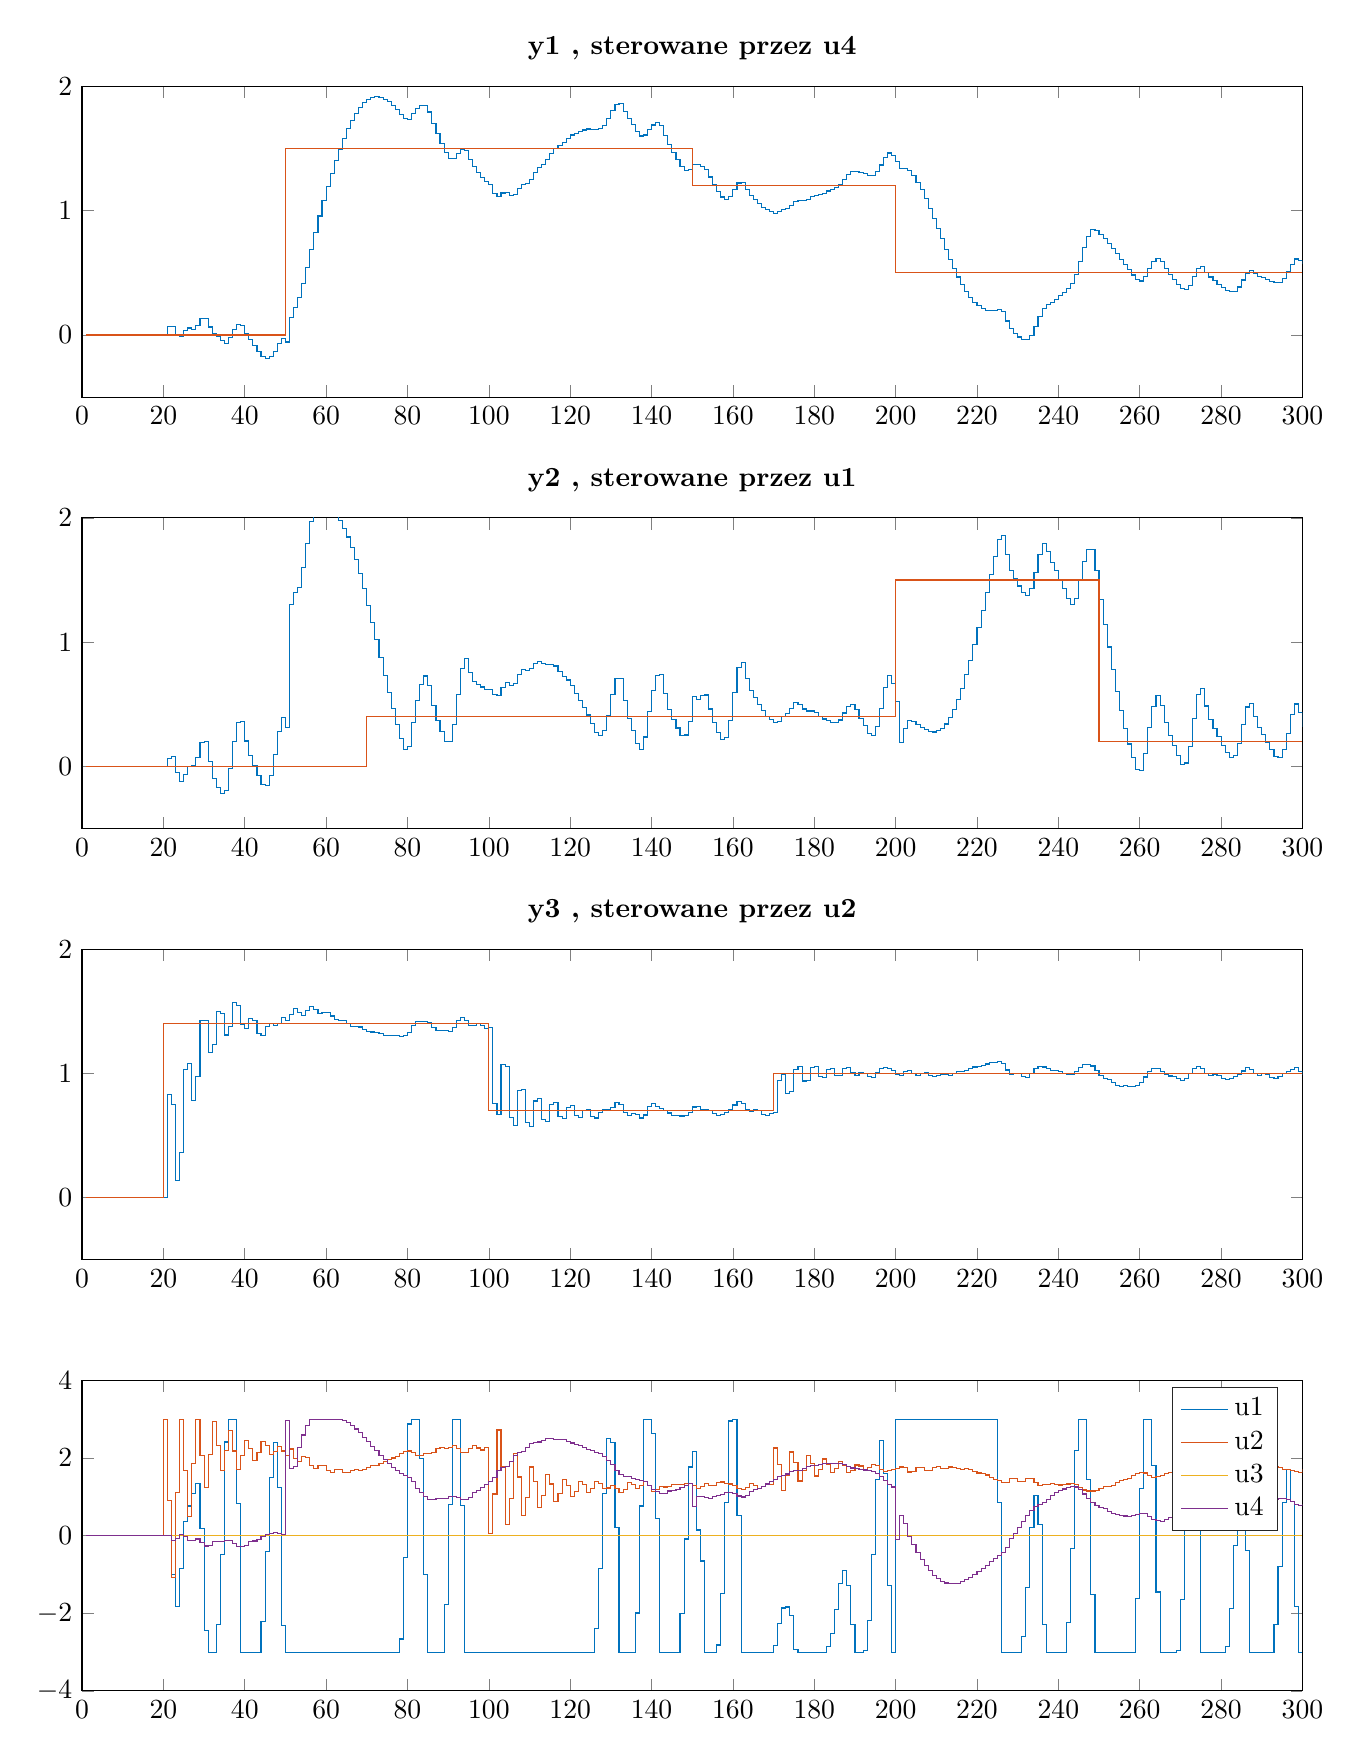
\begin{tikzpicture}

\begin{axis}[%
width=6.102in,
height=1.553in,
at={(1.024in,7.552in)},
scale only axis,
xmin=0,
xmax=300,
ymin=-0.5,
ymax=2,
axis background/.style={fill=white},
title style={font=\bfseries},
title={y1 , sterowane przez u4}
]
\addplot[const plot, color=mycolor1, forget plot] table[row sep=crcr] {%
1	0\\
2	0\\
3	0\\
4	0\\
5	0\\
6	0\\
7	0\\
8	0\\
9	0\\
10	0\\
11	0\\
12	0\\
13	0\\
14	0\\
15	0\\
16	0\\
17	0\\
18	0\\
19	0\\
20	0\\
21	0.0663597650785785\\
22	0.071588966531205\\
23	0.00499503121281067\\
24	-0.0125941951178842\\
25	0.0340712303003723\\
26	0.0558492606969018\\
27	0.0458404854290462\\
28	0.0748630481310482\\
29	0.131627908475342\\
30	0.133480048082829\\
31	0.0640299211767103\\
32	0.0114919064834567\\
33	-0.0148548695963331\\
34	-0.0470768952216941\\
35	-0.0653360629489498\\
36	-0.0193220616884297\\
37	0.0458664339151165\\
38	0.0874649720459928\\
39	0.0762878892567509\\
40	0.011988293254217\\
41	-0.0373530517270269\\
42	-0.0840038537279153\\
43	-0.134997160847272\\
44	-0.175695737357515\\
45	-0.190279439541588\\
46	-0.174240524426686\\
47	-0.130482081447082\\
48	-0.0713790413067126\\
49	-0.0316234485630056\\
50	-0.0564173443549718\\
51	0.137286666646813\\
52	0.224145191762096\\
53	0.303829424967543\\
54	0.413495060418247\\
55	0.545387597461219\\
56	0.68663279206694\\
57	0.827039251075882\\
58	0.957298338099073\\
59	1.08149135520723\\
60	1.1975003663685\\
61	1.30321986281943\\
62	1.40151079376904\\
63	1.49516865519523\\
64	1.58239709511536\\
65	1.65950639646999\\
66	1.72689856422163\\
67	1.78567828946602\\
68	1.83405841810684\\
69	1.87026452350106\\
70	1.89536661348405\\
71	1.91087916439432\\
72	1.91639807355308\\
73	1.91151023565425\\
74	1.89770169416179\\
75	1.87676032995215\\
76	1.84914676988913\\
77	1.81523731337639\\
78	1.77661824206869\\
79	1.74052504720969\\
80	1.7365085337493\\
81	1.78487711853722\\
82	1.82476122940984\\
83	1.84875754022748\\
84	1.84876085295764\\
85	1.79495237222474\\
86	1.70534676422339\\
87	1.62095258358137\\
88	1.54438252441271\\
89	1.4714478308283\\
90	1.42244179999858\\
91	1.42197782027602\\
92	1.46031720414949\\
93	1.49359298771413\\
94	1.48403882119872\\
95	1.41405876937434\\
96	1.35470039735732\\
97	1.30978445586273\\
98	1.26943805736818\\
99	1.23426868541058\\
100	1.20862260727031\\
101	1.14169060112049\\
102	1.11503944460033\\
103	1.1430087770464\\
104	1.14988785636305\\
105	1.12558066973335\\
106	1.13245390073394\\
107	1.17816767698198\\
108	1.21029429780043\\
109	1.22058247897089\\
110	1.25022817205551\\
111	1.30452046004585\\
112	1.34785116738524\\
113	1.37370027361521\\
114	1.40939460729946\\
115	1.45882610283172\\
116	1.49808344946013\\
117	1.52239572795009\\
118	1.55014462829019\\
119	1.58443031937404\\
120	1.60944933928797\\
121	1.62196691354103\\
122	1.63455679635879\\
123	1.64982128545148\\
124	1.65749560048603\\
125	1.65553898690791\\
126	1.65267593956998\\
127	1.66101218398282\\
128	1.68896219892634\\
129	1.73916299657701\\
130	1.80424930395742\\
131	1.8577874266909\\
132	1.86138727991066\\
133	1.80212596400872\\
134	1.74435101768808\\
135	1.69404972400005\\
136	1.64109957196125\\
137	1.60142765343463\\
138	1.60991571786693\\
139	1.65561117447508\\
140	1.69039362943391\\
141	1.70701668986953\\
142	1.68537689098911\\
143	1.60824273255904\\
144	1.53446253060244\\
145	1.47001641469787\\
146	1.41122237068954\\
147	1.35767239993366\\
148	1.32621921227757\\
149	1.33314065400145\\
150	1.37380125419064\\
151	1.37273428699585\\
152	1.35803522278079\\
153	1.33338616584782\\
154	1.27156016836132\\
155	1.21015568196713\\
156	1.15605573565219\\
157	1.11080682785369\\
158	1.09173360711427\\
159	1.11415115001528\\
160	1.17090132486071\\
161	1.22337786560214\\
162	1.22776325125285\\
163	1.17273644200149\\
164	1.12583705813027\\
165	1.09133889720006\\
166	1.05940213820376\\
167	1.02955224947621\\
168	1.006384618424\\
169	0.990504219066142\\
170	0.978790747629092\\
171	0.995041938268514\\
172	1.01175410843055\\
173	1.01922867882256\\
174	1.04041304205663\\
175	1.07430972184075\\
176	1.08483131307315\\
177	1.08260831356397\\
178	1.09131460625145\\
179	1.11164979483973\\
180	1.12534119304452\\
181	1.13028359242173\\
182	1.14081839078147\\
183	1.15848209380977\\
184	1.17351075813194\\
185	1.18744480953254\\
186	1.21340863766431\\
187	1.25297732477005\\
188	1.29066251806494\\
189	1.31243106181531\\
190	1.31512211913324\\
191	1.30721150452824\\
192	1.29738370179271\\
193	1.28502584664809\\
194	1.28517755252245\\
195	1.31363842784512\\
196	1.3683970732309\\
197	1.4289949381354\\
198	1.46507964878541\\
199	1.44579448335843\\
200	1.39501003839773\\
201	1.33842021522168\\
202	1.33815741686095\\
203	1.32217514193115\\
204	1.28142103262064\\
205	1.22819750417029\\
206	1.16793365702309\\
207	1.09884726922179\\
208	1.02086018666445\\
209	0.938765172728231\\
210	0.856325331126562\\
211	0.773306067146314\\
212	0.690063903820807\\
213	0.609977948966053\\
214	0.535675138183719\\
215	0.466963459642649\\
216	0.403877994998233\\
217	0.348383649254799\\
218	0.301884674857345\\
219	0.263807243667324\\
220	0.23363683632266\\
221	0.212113697496853\\
222	0.199595274707023\\
223	0.195089319511524\\
224	0.197619610921696\\
225	0.207031788476035\\
226	0.187928062495137\\
227	0.112121505754112\\
228	0.0505547368748533\\
229	0.0108997673901335\\
230	-0.0167091759550437\\
231	-0.0353374461861235\\
232	-0.0352305977730565\\
233	-0.00139124626089121\\
234	0.0656055026439446\\
235	0.147162981002298\\
236	0.215323215176872\\
237	0.24210460385859\\
238	0.260675713670134\\
239	0.286251004488848\\
240	0.314611783161238\\
241	0.343001925335311\\
242	0.371694871516389\\
243	0.413133902015624\\
244	0.484757756797275\\
245	0.591952833318584\\
246	0.700977656677381\\
247	0.794234075351718\\
248	0.849052343402841\\
249	0.844288556809833\\
250	0.808857257116126\\
251	0.77345760526119\\
252	0.736950273278301\\
253	0.695947776689668\\
254	0.652191012703222\\
255	0.608627229305931\\
256	0.565902950150851\\
257	0.523615116165359\\
258	0.482864917230042\\
259	0.445418368439061\\
260	0.43408380835034\\
261	0.471942984035941\\
262	0.536197105169876\\
263	0.591150247687086\\
264	0.618347290218314\\
265	0.588633817653723\\
266	0.534435162584689\\
267	0.487779880366096\\
268	0.446758676076589\\
269	0.407770672768815\\
270	0.372747834275888\\
271	0.365059102002798\\
272	0.40068905447637\\
273	0.470006989204404\\
274	0.533542142191624\\
275	0.551173182703901\\
276	0.50602313661346\\
277	0.466447540128391\\
278	0.4371996683262\\
279	0.409533759722326\\
280	0.38302397422074\\
281	0.361257237447557\\
282	0.347039887949319\\
283	0.352218707429091\\
284	0.385965216887131\\
285	0.442850663069576\\
286	0.498770358278946\\
287	0.51980391705352\\
288	0.494451082959045\\
289	0.473369288111783\\
290	0.45995502655925\\
291	0.4463878001704\\
292	0.432120385525771\\
293	0.420863269496035\\
294	0.424798662179646\\
295	0.45404197189548\\
296	0.507673028635954\\
297	0.570010907605893\\
298	0.611888767717936\\
299	0.602419334240914\\
300	0.571755912696899\\
};
\addplot[const plot, color=mycolor2, forget plot] table[row sep=crcr] {%
1	0\\
2	0\\
3	0\\
4	0\\
5	0\\
6	0\\
7	0\\
8	0\\
9	0\\
10	0\\
11	0\\
12	0\\
13	0\\
14	0\\
15	0\\
16	0\\
17	0\\
18	0\\
19	0\\
20	0\\
21	0\\
22	0\\
23	0\\
24	0\\
25	0\\
26	0\\
27	0\\
28	0\\
29	0\\
30	0\\
31	0\\
32	0\\
33	0\\
34	0\\
35	0\\
36	0\\
37	0\\
38	0\\
39	0\\
40	0\\
41	0\\
42	0\\
43	0\\
44	0\\
45	0\\
46	0\\
47	0\\
48	0\\
49	0\\
50	1.5\\
51	1.5\\
52	1.5\\
53	1.5\\
54	1.5\\
55	1.5\\
56	1.5\\
57	1.5\\
58	1.5\\
59	1.5\\
60	1.5\\
61	1.5\\
62	1.5\\
63	1.5\\
64	1.5\\
65	1.5\\
66	1.5\\
67	1.5\\
68	1.5\\
69	1.5\\
70	1.5\\
71	1.5\\
72	1.5\\
73	1.5\\
74	1.5\\
75	1.5\\
76	1.5\\
77	1.5\\
78	1.5\\
79	1.5\\
80	1.5\\
81	1.5\\
82	1.5\\
83	1.5\\
84	1.5\\
85	1.5\\
86	1.5\\
87	1.5\\
88	1.5\\
89	1.5\\
90	1.5\\
91	1.5\\
92	1.5\\
93	1.5\\
94	1.5\\
95	1.5\\
96	1.5\\
97	1.5\\
98	1.5\\
99	1.5\\
100	1.5\\
101	1.5\\
102	1.5\\
103	1.5\\
104	1.5\\
105	1.5\\
106	1.5\\
107	1.5\\
108	1.5\\
109	1.5\\
110	1.5\\
111	1.5\\
112	1.5\\
113	1.5\\
114	1.5\\
115	1.5\\
116	1.5\\
117	1.5\\
118	1.5\\
119	1.5\\
120	1.5\\
121	1.5\\
122	1.5\\
123	1.5\\
124	1.5\\
125	1.5\\
126	1.5\\
127	1.5\\
128	1.5\\
129	1.5\\
130	1.5\\
131	1.5\\
132	1.5\\
133	1.5\\
134	1.5\\
135	1.5\\
136	1.5\\
137	1.5\\
138	1.5\\
139	1.5\\
140	1.5\\
141	1.5\\
142	1.5\\
143	1.5\\
144	1.5\\
145	1.5\\
146	1.5\\
147	1.5\\
148	1.5\\
149	1.5\\
150	1.2\\
151	1.2\\
152	1.2\\
153	1.2\\
154	1.2\\
155	1.2\\
156	1.2\\
157	1.2\\
158	1.2\\
159	1.2\\
160	1.2\\
161	1.2\\
162	1.2\\
163	1.2\\
164	1.2\\
165	1.2\\
166	1.2\\
167	1.2\\
168	1.2\\
169	1.2\\
170	1.2\\
171	1.2\\
172	1.2\\
173	1.2\\
174	1.2\\
175	1.2\\
176	1.2\\
177	1.2\\
178	1.2\\
179	1.2\\
180	1.2\\
181	1.2\\
182	1.2\\
183	1.2\\
184	1.2\\
185	1.2\\
186	1.2\\
187	1.2\\
188	1.2\\
189	1.2\\
190	1.2\\
191	1.2\\
192	1.2\\
193	1.2\\
194	1.2\\
195	1.2\\
196	1.2\\
197	1.2\\
198	1.2\\
199	1.2\\
200	0.5\\
201	0.5\\
202	0.5\\
203	0.5\\
204	0.5\\
205	0.5\\
206	0.5\\
207	0.5\\
208	0.5\\
209	0.5\\
210	0.5\\
211	0.5\\
212	0.5\\
213	0.5\\
214	0.5\\
215	0.5\\
216	0.5\\
217	0.5\\
218	0.5\\
219	0.5\\
220	0.5\\
221	0.5\\
222	0.5\\
223	0.5\\
224	0.5\\
225	0.5\\
226	0.5\\
227	0.5\\
228	0.5\\
229	0.5\\
230	0.5\\
231	0.5\\
232	0.5\\
233	0.5\\
234	0.5\\
235	0.5\\
236	0.5\\
237	0.5\\
238	0.5\\
239	0.5\\
240	0.5\\
241	0.5\\
242	0.5\\
243	0.5\\
244	0.5\\
245	0.5\\
246	0.5\\
247	0.5\\
248	0.5\\
249	0.5\\
250	0.5\\
251	0.5\\
252	0.5\\
253	0.5\\
254	0.5\\
255	0.5\\
256	0.5\\
257	0.5\\
258	0.5\\
259	0.5\\
260	0.5\\
261	0.5\\
262	0.5\\
263	0.5\\
264	0.5\\
265	0.5\\
266	0.5\\
267	0.5\\
268	0.5\\
269	0.5\\
270	0.5\\
271	0.5\\
272	0.5\\
273	0.5\\
274	0.5\\
275	0.5\\
276	0.5\\
277	0.5\\
278	0.5\\
279	0.5\\
280	0.5\\
281	0.5\\
282	0.5\\
283	0.5\\
284	0.5\\
285	0.5\\
286	0.5\\
287	0.5\\
288	0.5\\
289	0.5\\
290	0.5\\
291	0.5\\
292	0.5\\
293	0.5\\
294	0.5\\
295	0.5\\
296	0.5\\
297	0.5\\
298	0.5\\
299	0.5\\
300	0.5\\
};
\end{axis}

\begin{axis}[%
width=6.102in,
height=1.553in,
at={(1.024in,5.395in)},
scale only axis,
xmin=0,
xmax=300,
ymin=-0.5,
ymax=2,
axis background/.style={fill=white},
title style={font=\bfseries},
title={y2 , sterowane przez u1}
]
\addplot[const plot, color=mycolor1, forget plot] table[row sep=crcr] {%
1	0\\
2	0\\
3	0\\
4	0\\
5	0\\
6	0\\
7	0\\
8	0\\
9	0\\
10	0\\
11	0\\
12	0\\
13	0\\
14	0\\
15	0\\
16	0\\
17	0\\
18	0\\
19	0\\
20	0\\
21	0.0612158143362928\\
22	0.0770823080206103\\
23	-0.0458429363644009\\
24	-0.122729839976068\\
25	-0.0632745444074269\\
26	-0.00375139118870736\\
27	0.00616287303807626\\
28	0.0733502584408069\\
29	0.191490452423229\\
30	0.199688457069445\\
31	0.0359528132083949\\
32	-0.0999725024965371\\
33	-0.167007944346612\\
34	-0.215274209649625\\
35	-0.196706796000686\\
36	-0.0142638841671194\\
37	0.197467674860574\\
38	0.349687774418878\\
39	0.362731603263329\\
40	0.204376875200392\\
41	0.0897091657995188\\
42	0.0105216762032766\\
43	-0.0761931103005929\\
44	-0.14731488640047\\
45	-0.155168921887421\\
46	-0.0706151928604203\\
47	0.0939724161253211\\
48	0.283871268953512\\
49	0.396156460428243\\
50	0.314527578915063\\
51	1.30059847194902\\
52	1.39837321213742\\
53	1.4396901074549\\
54	1.6040553842064\\
55	1.79628024526933\\
56	1.97062096938704\\
57	2.10439271571545\\
58	2.15382648651706\\
59	2.15619447638227\\
60	2.13017512586564\\
61	2.08584235053905\\
62	2.03248138115404\\
63	1.97674844932458\\
64	1.9179183530898\\
65	1.84584600507291\\
66	1.75955276384142\\
67	1.66180713477826\\
68	1.5517550962025\\
69	1.42868586840107\\
70	1.29631215196548\\
71	1.15906597669615\\
72	1.0182631865782\\
73	0.874843024963775\\
74	0.73232356726025\\
75	0.594424480174807\\
76	0.462502864175367\\
77	0.337384819358526\\
78	0.221410532004689\\
79	0.133253378064223\\
80	0.158846374761694\\
81	0.354180884224449\\
82	0.527951053294203\\
83	0.655621597346102\\
84	0.72744833399646\\
85	0.652351185632534\\
86	0.489397054434454\\
87	0.366068340342553\\
88	0.277414878650621\\
89	0.200497119159473\\
90	0.197210937689416\\
91	0.336354844140531\\
92	0.57907566583828\\
93	0.791251325166741\\
94	0.865376620546476\\
95	0.756859644573922\\
96	0.684000040108317\\
97	0.660401848242194\\
98	0.638798296591715\\
99	0.620495068997448\\
100	0.615822268826086\\
101	0.577345794709465\\
102	0.568687515169951\\
103	0.637480774220716\\
104	0.673087051947876\\
105	0.653025418125142\\
106	0.670215125599342\\
107	0.738453558435841\\
108	0.777622543067048\\
109	0.772660372673133\\
110	0.786242888002253\\
111	0.828655577553723\\
112	0.846393326775298\\
113	0.828766548618598\\
114	0.818197024405993\\
115	0.822928799326772\\
116	0.807816166166313\\
117	0.765776967821491\\
118	0.725942534365231\\
119	0.695119242303472\\
120	0.650548018778877\\
121	0.587775754073255\\
122	0.526958324478438\\
123	0.47362077376035\\
124	0.413092119213874\\
125	0.342570454026634\\
126	0.275918090184989\\
127	0.246834658000763\\
128	0.289851296429365\\
129	0.411505012802907\\
130	0.578251187167872\\
131	0.710007855774576\\
132	0.703890158087454\\
133	0.531290087796633\\
134	0.38668773564383\\
135	0.285295280332288\\
136	0.185641995586928\\
137	0.137193671410114\\
138	0.236738312546257\\
139	0.443274422703744\\
140	0.612671824959923\\
141	0.729692797255663\\
142	0.737816859795106\\
143	0.585417883363279\\
144	0.460302821610273\\
145	0.379460686718045\\
146	0.309100712445004\\
147	0.249302971140601\\
148	0.252226199877225\\
149	0.362791365879001\\
150	0.559936728402943\\
151	0.53463615865233\\
152	0.570192535308124\\
153	0.574469889025991\\
154	0.461690903258802\\
155	0.353556248888469\\
156	0.276109679542012\\
157	0.21878803201725\\
158	0.235123710677405\\
159	0.371178006901362\\
160	0.597620668533285\\
161	0.795192767124804\\
162	0.838997475292283\\
163	0.706894323445005\\
164	0.608301878028704\\
165	0.554144982941898\\
166	0.499991566869415\\
167	0.446447816618994\\
168	0.404457300285088\\
169	0.375068009545514\\
170	0.35257868420405\\
171	0.363243058298733\\
172	0.399024539831204\\
173	0.426667933419409\\
174	0.465407036457467\\
175	0.511351580192353\\
176	0.49783562713678\\
177	0.462065136277754\\
178	0.446057375062175\\
179	0.445358622097929\\
180	0.431954556684566\\
181	0.403128815083596\\
182	0.381213790658588\\
183	0.369451927003014\\
184	0.356661247061217\\
185	0.349562222094054\\
186	0.3728472929345\\
187	0.429428662232509\\
188	0.484709832434605\\
189	0.499398065781999\\
190	0.4578002730946\\
191	0.387971894400722\\
192	0.325728853381509\\
193	0.268068390086926\\
194	0.250627782426905\\
195	0.318955252857282\\
196	0.468221016668719\\
197	0.636047839635961\\
198	0.730026845648756\\
199	0.663549447545981\\
200	0.51976873296374\\
201	0.19176263831431\\
202	0.307980993182722\\
203	0.370721320786893\\
204	0.357969557823703\\
205	0.334408886969977\\
206	0.315882932864377\\
207	0.298542718820412\\
208	0.282871466573266\\
209	0.276617373876572\\
210	0.285112925374005\\
211	0.30688426558402\\
212	0.340771480630833\\
213	0.389933505324849\\
214	0.456274396958413\\
215	0.537207739306565\\
216	0.630293789512872\\
217	0.736040860297969\\
218	0.854238438613263\\
219	0.981738352338502\\
220	1.11555094530594\\
221	1.25479967542723\\
222	1.39830573518517\\
223	1.54306519831983\\
224	1.68630978162848\\
225	1.82675824364798\\
226	1.85891027956619\\
227	1.70193606066893\\
228	1.57782163584066\\
229	1.51023582931445\\
230	1.45186681110269\\
231	1.3981571786421\\
232	1.37714253020113\\
233	1.43106622121911\\
234	1.55978545470315\\
235	1.70790249217344\\
236	1.79145527866818\\
237	1.73241164145272\\
238	1.6418943191199\\
239	1.57377809343331\\
240	1.50607970201309\\
241	1.42999806819321\\
242	1.34989323659493\\
243	1.3051561186457\\
244	1.34977446929068\\
245	1.49822335398908\\
246	1.64743080725617\\
247	1.74766356667555\\
248	1.74313607200562\\
249	1.57748562239242\\
250	1.34613700199381\\
251	1.14482830636989\\
252	0.960702251248003\\
253	0.778773629565347\\
254	0.605499817780699\\
255	0.447763149665891\\
256	0.3064513521078\\
257	0.180096450975781\\
258	0.0692359089121674\\
259	-0.0247549983315055\\
260	-0.0359883296813051\\
261	0.102132630404388\\
262	0.313053826968042\\
263	0.48511070250655\\
264	0.570944392307357\\
265	0.491954332086436\\
266	0.350164950790647\\
267	0.247054340921092\\
268	0.164938309163996\\
269	0.0862106293220414\\
270	0.0175306675543557\\
271	0.0271760064735554\\
272	0.161188110341408\\
273	0.385361638374423\\
274	0.578806171787868\\
275	0.625135254432311\\
276	0.485573747653838\\
277	0.374641725567604\\
278	0.30695889919367\\
279	0.238674718980308\\
280	0.170593309806656\\
281	0.112571476716544\\
282	0.0724345804473119\\
283	0.0876529707727999\\
284	0.183963976280323\\
285	0.338513142677558\\
286	0.478069895648506\\
287	0.507155795087644\\
288	0.399260078488718\\
289	0.31198613964231\\
290	0.255590235122561\\
291	0.196540334809167\\
292	0.135285003517338\\
293	0.080864289094379\\
294	0.069235741674804\\
295	0.13324788314036\\
296	0.266940927566105\\
297	0.418388030011103\\
298	0.502179194217037\\
299	0.434785724784997\\
300	0.315068597130074\\
};
\addplot[const plot, color=mycolor2, forget plot] table[row sep=crcr] {%
1	0\\
2	0\\
3	0\\
4	0\\
5	0\\
6	0\\
7	0\\
8	0\\
9	0\\
10	0\\
11	0\\
12	0\\
13	0\\
14	0\\
15	0\\
16	0\\
17	0\\
18	0\\
19	0\\
20	0\\
21	0\\
22	0\\
23	0\\
24	0\\
25	0\\
26	0\\
27	0\\
28	0\\
29	0\\
30	0\\
31	0\\
32	0\\
33	0\\
34	0\\
35	0\\
36	0\\
37	0\\
38	0\\
39	0\\
40	0\\
41	0\\
42	0\\
43	0\\
44	0\\
45	0\\
46	0\\
47	0\\
48	0\\
49	0\\
50	0\\
51	0\\
52	0\\
53	0\\
54	0\\
55	0\\
56	0\\
57	0\\
58	0\\
59	0\\
60	0\\
61	0\\
62	0\\
63	0\\
64	0\\
65	0\\
66	0\\
67	0\\
68	0\\
69	0\\
70	0.4\\
71	0.4\\
72	0.4\\
73	0.4\\
74	0.4\\
75	0.4\\
76	0.4\\
77	0.4\\
78	0.4\\
79	0.4\\
80	0.4\\
81	0.4\\
82	0.4\\
83	0.4\\
84	0.4\\
85	0.4\\
86	0.4\\
87	0.4\\
88	0.4\\
89	0.4\\
90	0.4\\
91	0.4\\
92	0.4\\
93	0.4\\
94	0.4\\
95	0.4\\
96	0.4\\
97	0.4\\
98	0.4\\
99	0.4\\
100	0.4\\
101	0.4\\
102	0.4\\
103	0.4\\
104	0.4\\
105	0.4\\
106	0.4\\
107	0.4\\
108	0.4\\
109	0.4\\
110	0.4\\
111	0.4\\
112	0.4\\
113	0.4\\
114	0.4\\
115	0.4\\
116	0.4\\
117	0.4\\
118	0.4\\
119	0.4\\
120	0.4\\
121	0.4\\
122	0.4\\
123	0.4\\
124	0.4\\
125	0.4\\
126	0.4\\
127	0.4\\
128	0.4\\
129	0.4\\
130	0.4\\
131	0.4\\
132	0.4\\
133	0.4\\
134	0.4\\
135	0.4\\
136	0.4\\
137	0.4\\
138	0.4\\
139	0.4\\
140	0.4\\
141	0.4\\
142	0.4\\
143	0.4\\
144	0.4\\
145	0.4\\
146	0.4\\
147	0.4\\
148	0.4\\
149	0.4\\
150	0.4\\
151	0.4\\
152	0.4\\
153	0.4\\
154	0.4\\
155	0.4\\
156	0.4\\
157	0.4\\
158	0.4\\
159	0.4\\
160	0.4\\
161	0.4\\
162	0.4\\
163	0.4\\
164	0.4\\
165	0.4\\
166	0.4\\
167	0.4\\
168	0.4\\
169	0.4\\
170	0.4\\
171	0.4\\
172	0.4\\
173	0.4\\
174	0.4\\
175	0.4\\
176	0.4\\
177	0.4\\
178	0.4\\
179	0.4\\
180	0.4\\
181	0.4\\
182	0.4\\
183	0.4\\
184	0.4\\
185	0.4\\
186	0.4\\
187	0.4\\
188	0.4\\
189	0.4\\
190	0.4\\
191	0.4\\
192	0.4\\
193	0.4\\
194	0.4\\
195	0.4\\
196	0.4\\
197	0.4\\
198	0.4\\
199	0.4\\
200	1.5\\
201	1.5\\
202	1.5\\
203	1.5\\
204	1.5\\
205	1.5\\
206	1.5\\
207	1.5\\
208	1.5\\
209	1.5\\
210	1.5\\
211	1.5\\
212	1.5\\
213	1.5\\
214	1.5\\
215	1.5\\
216	1.5\\
217	1.5\\
218	1.5\\
219	1.5\\
220	1.5\\
221	1.5\\
222	1.5\\
223	1.5\\
224	1.5\\
225	1.5\\
226	1.5\\
227	1.5\\
228	1.5\\
229	1.5\\
230	1.5\\
231	1.5\\
232	1.5\\
233	1.5\\
234	1.5\\
235	1.5\\
236	1.5\\
237	1.5\\
238	1.5\\
239	1.5\\
240	1.5\\
241	1.5\\
242	1.5\\
243	1.5\\
244	1.5\\
245	1.5\\
246	1.5\\
247	1.5\\
248	1.5\\
249	1.5\\
250	0.2\\
251	0.2\\
252	0.2\\
253	0.2\\
254	0.2\\
255	0.2\\
256	0.2\\
257	0.2\\
258	0.2\\
259	0.2\\
260	0.2\\
261	0.2\\
262	0.2\\
263	0.2\\
264	0.2\\
265	0.2\\
266	0.2\\
267	0.2\\
268	0.2\\
269	0.2\\
270	0.2\\
271	0.2\\
272	0.2\\
273	0.2\\
274	0.2\\
275	0.2\\
276	0.2\\
277	0.2\\
278	0.2\\
279	0.2\\
280	0.2\\
281	0.2\\
282	0.2\\
283	0.2\\
284	0.2\\
285	0.2\\
286	0.2\\
287	0.2\\
288	0.2\\
289	0.2\\
290	0.2\\
291	0.2\\
292	0.2\\
293	0.2\\
294	0.2\\
295	0.2\\
296	0.2\\
297	0.2\\
298	0.2\\
299	0.2\\
300	0.2\\
};
\end{axis}

\begin{axis}[%
width=6.102in,
height=1.553in,
at={(1.024in,3.239in)},
scale only axis,
xmin=0,
xmax=300,
ymin=-0.5,
ymax=2,
axis background/.style={fill=white},
title style={font=\bfseries},
title={y3 , sterowane przez u2}
]
\addplot[const plot, color=mycolor1, forget plot] table[row sep=crcr] {%
1	0\\
2	0\\
3	0\\
4	0\\
5	0\\
6	0\\
7	0\\
8	0\\
9	0\\
10	0\\
11	0\\
12	0\\
13	0\\
14	0\\
15	0\\
16	0\\
17	0\\
18	0\\
19	0\\
20	0\\
21	0.82628561460347\\
22	0.749053243317543\\
23	0.140714565306018\\
24	0.364417282953638\\
25	1.02885645926881\\
26	1.07765949753952\\
27	0.779682715228037\\
28	0.977649410709241\\
29	1.42190753710126\\
30	1.42574404723797\\
31	1.16803635905784\\
32	1.23523972903852\\
33	1.4973532202228\\
34	1.48280785905785\\
35	1.30822496627074\\
36	1.37444944448603\\
37	1.56707027683148\\
38	1.54897284457788\\
39	1.39231906504701\\
40	1.36114738694015\\
41	1.44205248335092\\
42	1.42642021322767\\
43	1.32368847195416\\
44	1.30655829031549\\
45	1.37752020883852\\
46	1.40421808336146\\
47	1.38165497575957\\
48	1.40357725728331\\
49	1.45090178633027\\
50	1.42167993737501\\
51	1.47299244125324\\
52	1.51989011501428\\
53	1.48846587398506\\
54	1.46557157268338\\
55	1.50663281519752\\
56	1.53777455277206\\
57	1.51092559268829\\
58	1.48048983940114\\
59	1.48814512876277\\
60	1.49229453989871\\
61	1.4611315264026\\
62	1.43053872490173\\
63	1.42851111026865\\
64	1.42718995063636\\
65	1.40348292381995\\
66	1.37997701786522\\
67	1.37581662379634\\
68	1.3726946585481\\
69	1.35482976433768\\
70	1.33721146072276\\
71	1.33307526352637\\
72	1.33045009844988\\
73	1.3185962846962\\
74	1.30744441779914\\
75	1.30607736563597\\
76	1.30659197761189\\
77	1.30158460381358\\
78	1.29752601189435\\
79	1.303757443801\\
80	1.33182186168165\\
81	1.38550229665346\\
82	1.41847601837618\\
83	1.42021912930657\\
84	1.41982425775783\\
85	1.40746389475955\\
86	1.37164271844787\\
87	1.3464659466506\\
88	1.34569813734073\\
89	1.34229115557718\\
90	1.33789600876584\\
91	1.36775562023766\\
92	1.4236449011527\\
93	1.44965207607235\\
94	1.426566142697\\
95	1.38534227986195\\
96	1.38263530171559\\
97	1.39930145460483\\
98	1.38764380347901\\
99	1.36376557760348\\
100	1.36761322373139\\
101	0.759610046734967\\
102	0.668653362788754\\
103	1.07254439389731\\
104	1.05771810044881\\
105	0.641620952470713\\
106	0.577447858911882\\
107	0.859309170771733\\
108	0.869728936929094\\
109	0.606875476738369\\
110	0.574947479880371\\
111	0.777617977328062\\
112	0.79933006454931\\
113	0.631306908016182\\
114	0.61229670406299\\
115	0.751015861398012\\
116	0.768779438176033\\
117	0.65526341614977\\
118	0.638403906430672\\
119	0.728509884451737\\
120	0.738872693275539\\
121	0.659591309966392\\
122	0.643913422446944\\
123	0.701639321318437\\
124	0.707587546410823\\
125	0.652964902919867\\
126	0.640616921896221\\
127	0.684712004747606\\
128	0.710029047756627\\
129	0.706661401067698\\
130	0.72792963677933\\
131	0.764507249526561\\
132	0.750688597733867\\
133	0.685437210381062\\
134	0.658903646913095\\
135	0.678736978818462\\
136	0.671233471460063\\
137	0.640628976876399\\
138	0.664954289368777\\
139	0.733821905226549\\
140	0.755810554760703\\
141	0.731352806749709\\
142	0.717804932550726\\
143	0.704152359542872\\
144	0.681103625813298\\
145	0.663666283378193\\
146	0.659193136991589\\
147	0.656476711786337\\
148	0.659507324063569\\
149	0.68597265412851\\
150	0.728763518398897\\
151	0.732131716895686\\
152	0.71046209599062\\
153	0.709771274954816\\
154	0.703643121324237\\
155	0.679122351496732\\
156	0.66281716379889\\
157	0.66737574202039\\
158	0.682757806065994\\
159	0.707933167375212\\
160	0.745507178995187\\
161	0.771490288576365\\
162	0.755429815180352\\
163	0.707650211883444\\
164	0.692141838174098\\
165	0.706559292229408\\
166	0.697797123291198\\
167	0.668440233640242\\
168	0.662934182919025\\
169	0.679572413374077\\
170	0.681431083797992\\
171	0.938993986138766\\
172	0.987339779021366\\
173	0.835754861827651\\
174	0.854303327712261\\
175	1.03140434594491\\
176	1.05480469487122\\
177	0.938226854805387\\
178	0.939410637921881\\
179	1.04952229060242\\
180	1.05809712386055\\
181	0.97170972354102\\
182	0.964062933808302\\
183	1.03230321243365\\
184	1.03625306634961\\
185	0.979637857644113\\
186	0.980021702105829\\
187	1.03589673312318\\
188	1.04650431220125\\
189	1.00436021503553\\
190	0.985911066021479\\
191	1.00229469899714\\
192	0.999941495850812\\
193	0.970936099906888\\
194	0.966607976001544\\
195	1.00274318779527\\
196	1.03784582899262\\
197	1.04634646558229\\
198	1.04089117199969\\
199	1.02169251210846\\
200	0.992525864061369\\
201	0.980631328865459\\
202	1.01138699122496\\
203	1.02611078502226\\
204	0.998880388954774\\
205	0.981449659528584\\
206	0.997015908464317\\
207	1.00417792586586\\
208	0.984619109124871\\
209	0.97314426918291\\
210	0.985880717670243\\
211	0.994999506915414\\
212	0.987351310714148\\
213	0.985715902882542\\
214	1.00095059137252\\
215	1.0141872326405\\
216	1.01594063196167\\
217	1.02108569286105\\
218	1.03696845736957\\
219	1.05088185332046\\
220	1.05612365936655\\
221	1.06251453555185\\
222	1.07514746164413\\
223	1.08559132742789\\
224	1.08924092061538\\
225	1.09266406706479\\
226	1.07897704828969\\
227	1.0268043485638\\
228	0.992024180060544\\
229	0.998977604570637\\
230	1.0006076915344\\
231	0.976600598613447\\
232	0.968977749382279\\
233	1.00165937902842\\
234	1.04046557008756\\
235	1.054135226948\\
236	1.05082503235878\\
237	1.03682581395885\\
238	1.02484469509265\\
239	1.02071081845324\\
240	1.01444314351648\\
241	1.00155590051889\\
242	0.991088900889203\\
243	0.994604140859153\\
244	1.01581633591125\\
245	1.04891328162976\\
246	1.07035365967456\\
247	1.0725118095776\\
248	1.05911238495961\\
249	1.02363163506571\\
250	0.981535838372694\\
251	0.95913445300792\\
252	0.947225744802442\\
253	0.925390279169066\\
254	0.90252192301506\\
255	0.896151190940589\\
256	0.899017923943633\\
257	0.896057713876046\\
258	0.892158929072715\\
259	0.898617600898688\\
260	0.923508342247906\\
261	0.970213723517333\\
262	1.01737817873973\\
263	1.03865325611614\\
264	1.03699494299488\\
265	1.01452553128571\\
266	0.988450979463067\\
267	0.978701618786842\\
268	0.974246947570239\\
269	0.959680736194184\\
270	0.945742882031122\\
271	0.958422907969199\\
272	0.998546918234149\\
273	1.03911475340166\\
274	1.05404564744287\\
275	1.03803437881683\\
276	0.99975318047436\\
277	0.983953322836798\\
278	0.989866159741287\\
279	0.980148873655854\\
280	0.956312596847778\\
281	0.950009262072611\\
282	0.961709664247373\\
283	0.973277336727339\\
284	0.989044458991555\\
285	1.01883360207035\\
286	1.04338582733682\\
287	1.0332028913734\\
288	0.995340781938442\\
289	0.983025632013354\\
290	0.995260681294761\\
291	0.988063777238584\\
292	0.962873726746187\\
293	0.95662829917903\\
294	0.975497596744563\\
295	0.996466462755801\\
296	1.01353649152289\\
297	1.03412390935088\\
298	1.04402788014031\\
299	1.01786956369979\\
300	0.984123781627473\\
};
\addplot[const plot, color=mycolor2, forget plot] table[row sep=crcr] {%
1	0\\
2	0\\
3	0\\
4	0\\
5	0\\
6	0\\
7	0\\
8	0\\
9	0\\
10	0\\
11	0\\
12	0\\
13	0\\
14	0\\
15	0\\
16	0\\
17	0\\
18	0\\
19	0\\
20	1.4\\
21	1.4\\
22	1.4\\
23	1.4\\
24	1.4\\
25	1.4\\
26	1.4\\
27	1.4\\
28	1.4\\
29	1.4\\
30	1.4\\
31	1.4\\
32	1.4\\
33	1.4\\
34	1.4\\
35	1.4\\
36	1.4\\
37	1.4\\
38	1.4\\
39	1.4\\
40	1.4\\
41	1.4\\
42	1.4\\
43	1.4\\
44	1.4\\
45	1.4\\
46	1.4\\
47	1.4\\
48	1.4\\
49	1.4\\
50	1.4\\
51	1.4\\
52	1.4\\
53	1.4\\
54	1.4\\
55	1.4\\
56	1.4\\
57	1.4\\
58	1.4\\
59	1.4\\
60	1.4\\
61	1.4\\
62	1.4\\
63	1.4\\
64	1.4\\
65	1.4\\
66	1.4\\
67	1.4\\
68	1.4\\
69	1.4\\
70	1.4\\
71	1.4\\
72	1.4\\
73	1.4\\
74	1.4\\
75	1.4\\
76	1.4\\
77	1.4\\
78	1.4\\
79	1.4\\
80	1.4\\
81	1.4\\
82	1.4\\
83	1.4\\
84	1.4\\
85	1.4\\
86	1.4\\
87	1.4\\
88	1.4\\
89	1.4\\
90	1.4\\
91	1.4\\
92	1.4\\
93	1.4\\
94	1.4\\
95	1.4\\
96	1.4\\
97	1.4\\
98	1.4\\
99	1.4\\
100	0.7\\
101	0.7\\
102	0.7\\
103	0.7\\
104	0.7\\
105	0.7\\
106	0.7\\
107	0.7\\
108	0.7\\
109	0.7\\
110	0.7\\
111	0.7\\
112	0.7\\
113	0.7\\
114	0.7\\
115	0.7\\
116	0.7\\
117	0.7\\
118	0.7\\
119	0.7\\
120	0.7\\
121	0.7\\
122	0.7\\
123	0.7\\
124	0.7\\
125	0.7\\
126	0.7\\
127	0.7\\
128	0.7\\
129	0.7\\
130	0.7\\
131	0.7\\
132	0.7\\
133	0.7\\
134	0.7\\
135	0.7\\
136	0.7\\
137	0.7\\
138	0.7\\
139	0.7\\
140	0.7\\
141	0.7\\
142	0.7\\
143	0.7\\
144	0.7\\
145	0.7\\
146	0.7\\
147	0.7\\
148	0.7\\
149	0.7\\
150	0.7\\
151	0.7\\
152	0.7\\
153	0.7\\
154	0.7\\
155	0.7\\
156	0.7\\
157	0.7\\
158	0.7\\
159	0.7\\
160	0.7\\
161	0.7\\
162	0.7\\
163	0.7\\
164	0.7\\
165	0.7\\
166	0.7\\
167	0.7\\
168	0.7\\
169	0.7\\
170	1\\
171	1\\
172	1\\
173	1\\
174	1\\
175	1\\
176	1\\
177	1\\
178	1\\
179	1\\
180	1\\
181	1\\
182	1\\
183	1\\
184	1\\
185	1\\
186	1\\
187	1\\
188	1\\
189	1\\
190	1\\
191	1\\
192	1\\
193	1\\
194	1\\
195	1\\
196	1\\
197	1\\
198	1\\
199	1\\
200	1\\
201	1\\
202	1\\
203	1\\
204	1\\
205	1\\
206	1\\
207	1\\
208	1\\
209	1\\
210	1\\
211	1\\
212	1\\
213	1\\
214	1\\
215	1\\
216	1\\
217	1\\
218	1\\
219	1\\
220	1\\
221	1\\
222	1\\
223	1\\
224	1\\
225	1\\
226	1\\
227	1\\
228	1\\
229	1\\
230	1\\
231	1\\
232	1\\
233	1\\
234	1\\
235	1\\
236	1\\
237	1\\
238	1\\
239	1\\
240	1\\
241	1\\
242	1\\
243	1\\
244	1\\
245	1\\
246	1\\
247	1\\
248	1\\
249	1\\
250	1\\
251	1\\
252	1\\
253	1\\
254	1\\
255	1\\
256	1\\
257	1\\
258	1\\
259	1\\
260	1\\
261	1\\
262	1\\
263	1\\
264	1\\
265	1\\
266	1\\
267	1\\
268	1\\
269	1\\
270	1\\
271	1\\
272	1\\
273	1\\
274	1\\
275	1\\
276	1\\
277	1\\
278	1\\
279	1\\
280	1\\
281	1\\
282	1\\
283	1\\
284	1\\
285	1\\
286	1\\
287	1\\
288	1\\
289	1\\
290	1\\
291	1\\
292	1\\
293	1\\
294	1\\
295	1\\
296	1\\
297	1\\
298	1\\
299	1\\
300	1\\
};
\end{axis}

\begin{axis}[%
width=6.102in,
height=1.553in,
at={(1.024in,1.083in)},
scale only axis,
xmin=0,
xmax=300,
ymin=-4,
ymax=4,
axis background/.style={fill=white},
legend style={legend cell align=left, align=left, draw=white!15!black}
]
\addplot[const plot, color=mycolor1] table[row sep=crcr] {%
1	0\\
2	0\\
3	0\\
4	0\\
5	0\\
6	0\\
7	0\\
8	0\\
9	0\\
10	0\\
11	0\\
12	0\\
13	0\\
14	0\\
15	0\\
16	0\\
17	0\\
18	0\\
19	0\\
20	0\\
21	0\\
22	-1.01006093654883\\
23	-1.82280041136671\\
24	-0.85556953721727\\
25	0.363156951531185\\
26	0.761770752619624\\
27	1.085488664034\\
28	1.335313091435\\
29	0.193763722079502\\
30	-2.45267904282619\\
31	-3\\
32	-3\\
33	-2.27893835216085\\
34	-0.48881791841614\\
35	2.4104819731823\\
36	3\\
37	3\\
38	0.815045009551257\\
39	-3\\
40	-3\\
41	-3\\
42	-3\\
43	-3\\
44	-2.20215610331275\\
45	-0.406038862179107\\
46	1.50654536276338\\
47	2.39181844920747\\
48	1.24267316801105\\
49	-2.31271849161946\\
50	-3\\
51	-3\\
52	-3\\
53	-3\\
54	-3\\
55	-3\\
56	-3\\
57	-3\\
58	-3\\
59	-3\\
60	-3\\
61	-3\\
62	-3\\
63	-3\\
64	-3\\
65	-3\\
66	-3\\
67	-3\\
68	-3\\
69	-3\\
70	-3\\
71	-3\\
72	-3\\
73	-3\\
74	-3\\
75	-3\\
76	-3\\
77	-3\\
78	-2.66462491914927\\
79	-0.562529737089901\\
80	2.87505959873444\\
81	3\\
82	3\\
83	1.99208600375886\\
84	-0.991122758091989\\
85	-3\\
86	-3\\
87	-3\\
88	-3\\
89	-1.76821527177281\\
90	0.807783809920211\\
91	3\\
92	3\\
93	0.784647218585871\\
94	-3\\
95	-3\\
96	-3\\
97	-3\\
98	-3\\
99	-3\\
100	-3\\
101	-3\\
102	-3\\
103	-3\\
104	-3\\
105	-3\\
106	-3\\
107	-3\\
108	-3\\
109	-3\\
110	-3\\
111	-3\\
112	-3\\
113	-3\\
114	-3\\
115	-3\\
116	-3\\
117	-3\\
118	-3\\
119	-3\\
120	-3\\
121	-3\\
122	-3\\
123	-3\\
124	-3\\
125	-3\\
126	-2.3959462398975\\
127	-0.857869038033319\\
128	1.08332205718172\\
129	2.49652705999297\\
130	2.39957112396067\\
131	0.205606353136398\\
132	-3\\
133	-3\\
134	-3\\
135	-3\\
136	-1.99495463493383\\
137	0.761540626511046\\
138	3\\
139	3\\
140	2.63834734102447\\
141	0.433390524186271\\
142	-3\\
143	-3\\
144	-3\\
145	-3\\
146	-3\\
147	-2.01602353461887\\
148	-0.0880313354095288\\
149	1.76540437550074\\
150	2.1752255107328\\
151	0.1438475369134\\
152	-0.654871813101982\\
153	-3\\
154	-3\\
155	-3\\
156	-2.81781566637467\\
157	-1.49209893170716\\
158	0.847383643242484\\
159	2.9520945799426\\
160	3\\
161	0.512351756896581\\
162	-3\\
163	-3\\
164	-3\\
165	-3\\
166	-3\\
167	-3\\
168	-3\\
169	-3\\
170	-2.83387930507678\\
171	-2.26516132456279\\
172	-1.86473971223458\\
173	-1.83979378743325\\
174	-2.06658898991186\\
175	-2.93994282980172\\
176	-3\\
177	-3\\
178	-3\\
179	-3\\
180	-3\\
181	-3\\
182	-3\\
183	-2.85828877284711\\
184	-2.51391502895902\\
185	-1.91521889689801\\
186	-1.22474777050885\\
187	-0.894978920590005\\
188	-1.28157048298197\\
189	-2.29565150901614\\
190	-3\\
191	-3\\
192	-2.96442260409441\\
193	-2.17596111545149\\
194	-0.483954517928777\\
195	1.43682687739018\\
196	2.44536323292526\\
197	1.60811415975957\\
198	-1.28874908636208\\
199	-3\\
200	3\\
201	3\\
202	3\\
203	3\\
204	3\\
205	3\\
206	3\\
207	3\\
208	3\\
209	3\\
210	3\\
211	3\\
212	3\\
213	3\\
214	3\\
215	3\\
216	3\\
217	3\\
218	3\\
219	3\\
220	3\\
221	3\\
222	3\\
223	3\\
224	2.99791918904819\\
225	0.856962368465971\\
226	-3\\
227	-3\\
228	-3\\
229	-3\\
230	-3\\
231	-2.59596347837994\\
232	-1.33797081859116\\
233	0.2141554062898\\
234	1.04118866083045\\
235	0.274870136164924\\
236	-2.29352740173781\\
237	-3\\
238	-3\\
239	-3\\
240	-3\\
241	-3\\
242	-2.24203892068972\\
243	-0.326770025135424\\
244	2.18236488251322\\
245	3\\
246	3\\
247	1.45542001944714\\
248	-1.51463790021268\\
249	-3\\
250	-3\\
251	-3\\
252	-3\\
253	-3\\
254	-3\\
255	-3\\
256	-3\\
257	-3\\
258	-3\\
259	-1.6303772273792\\
260	1.21677085607721\\
261	3\\
262	3\\
263	1.81653656114804\\
264	-1.45268211037604\\
265	-3\\
266	-3\\
267	-3\\
268	-3\\
269	-2.96956424904163\\
270	-1.63732835965189\\
271	0.730365490632571\\
272	2.89617761454433\\
273	3\\
274	0.687387755541242\\
275	-3\\
276	-3\\
277	-3\\
278	-3\\
279	-3\\
280	-3\\
281	-2.86648261461954\\
282	-1.87651047077444\\
283	-0.250954831620946\\
284	1.17060164368343\\
285	1.35798583317023\\
286	-0.373669023543855\\
287	-3\\
288	-3\\
289	-3\\
290	-3\\
291	-3\\
292	-3\\
293	-2.2916914577027\\
294	-0.790556710234915\\
295	0.861825699234631\\
296	1.69731795541345\\
297	0.87673732407659\\
298	-1.82409551320298\\
299	-3\\
300	-3\\
};
\addlegendentry{u1}

\addplot[const plot, color=mycolor2] table[row sep=crcr] {%
1	0\\
2	0\\
3	0\\
4	0\\
5	0\\
6	0\\
7	0\\
8	0\\
9	0\\
10	0\\
11	0\\
12	0\\
13	0\\
14	0\\
15	0\\
16	0\\
17	0\\
18	0\\
19	0\\
20	3\\
21	0.9\\
22	-1.08542824746128\\
23	1.10500538112319\\
24	3\\
25	1.68593152896918\\
26	0.49170099976329\\
27	1.84754124837941\\
28	3\\
29	2.0708133174491\\
30	1.23408309228281\\
31	2.09917691857193\\
32	2.93152790181179\\
33	2.31368339348537\\
34	1.67860142257857\\
35	2.20142421862183\\
36	2.69832396832111\\
37	2.17981614541181\\
38	1.69902267447668\\
39	2.05954585557604\\
40	2.45798935225521\\
41	2.24983021451727\\
42	1.9439716014985\\
43	2.13556043054512\\
44	2.42496394282368\\
45	2.31332931462526\\
46	2.09516357099035\\
47	2.16155921141759\\
48	2.28617601848886\\
49	2.17897490045315\\
50	2.06722611545635\\
51	2.23139528948976\\
52	1.99534598528745\\
53	1.90905733269392\\
54	2.04503640605383\\
55	2.01236146623333\\
56	1.8003380391173\\
57	1.72793346942957\\
58	1.80858878846489\\
59	1.79834427013644\\
60	1.67234815343627\\
61	1.63010058158634\\
62	1.69353192777121\\
63	1.70006674245553\\
64	1.63020152456042\\
65	1.61618450896488\\
66	1.67699505153547\\
67	1.70423373034554\\
68	1.68075469022731\\
69	1.69467197724819\\
70	1.76014162366152\\
71	1.80425643982032\\
72	1.81385674311737\\
73	1.84757850346001\\
74	1.91562801878152\\
75	1.96886581634154\\
76	1.99728279317813\\
77	2.03983751711206\\
78	2.10384471710247\\
79	2.15622809133656\\
80	2.1790957478543\\
81	2.14847053165501\\
82	2.06422702291708\\
83	2.07167214893513\\
84	2.12271647266872\\
85	2.11737646240964\\
86	2.14684577017764\\
87	2.23481191981424\\
88	2.2591727163081\\
89	2.23808157964534\\
90	2.27476958308676\\
91	2.31109426890795\\
92	2.23631223361891\\
93	2.13051348346983\\
94	2.14594627623473\\
95	2.24816387150773\\
96	2.32268648762243\\
97	2.25636530099705\\
98	2.2054686969565\\
99	2.27703764159147\\
100	0.0625046716958022\\
101	1.0703605812273\\
102	2.72025958685579\\
103	1.77005743232066\\
104	0.291171531931042\\
105	0.960866850907126\\
106	2.10467094471455\\
107	1.51022872658919\\
108	0.52710934647107\\
109	0.977313144793483\\
110	1.76756195426352\\
111	1.39218328530137\\
112	0.732174434940195\\
113	1.02814215770249\\
114	1.567976558603\\
115	1.32805995437652\\
116	0.883053933099822\\
117	1.0772526925423\\
118	1.44731719859567\\
119	1.29744685305533\\
120	1.00168145183334\\
121	1.13395933697224\\
122	1.39291310373681\\
123	1.30550781657352\\
124	1.1145861589788\\
125	1.20988656451231\\
126	1.39551283283728\\
127	1.34991603272228\\
128	1.21160259045988\\
129	1.22515636400953\\
130	1.28172077788828\\
131	1.20253301791377\\
132	1.11222742951886\\
133	1.1980396485763\\
134	1.3571250550206\\
135	1.32013775639535\\
136	1.22316047731042\\
137	1.29784505062672\\
138	1.3966859075768\\
139	1.28610516437105\\
140	1.12845889313365\\
141	1.17782006124992\\
142	1.27337976397361\\
143	1.25281845572346\\
144	1.26119110332566\\
145	1.30671816215963\\
146	1.32674024470792\\
147	1.32457014390508\\
148	1.34485566455315\\
149	1.35133496834847\\
150	1.29163020816009\\
151	1.21250423234696\\
152	1.27275755657372\\
153	1.33385436306092\\
154	1.28752924162184\\
155	1.30117846137221\\
156	1.36679309538832\\
157	1.38118224000293\\
158	1.35234790348793\\
159	1.32778548077252\\
160	1.28535078157577\\
161	1.20961938274168\\
162	1.17756871034521\\
163	1.24598632375643\\
164	1.34143418008918\\
165	1.29245208210901\\
166	1.21850768992352\\
167	1.27254000096862\\
168	1.3515269928122\\
169	1.32648776153413\\
170	2.25493431965326\\
171	1.8423838949986\\
172	1.16830626133992\\
173	1.55681124608364\\
174	2.15248392321773\\
175	1.87115414379149\\
176	1.40552110244846\\
177	1.66796983193081\\
178	2.06624616256177\\
179	1.8601297598988\\
180	1.53492913595909\\
181	1.70252308793004\\
182	1.9713832435545\\
183	1.83760564777626\\
184	1.61849969587428\\
185	1.72599162168132\\
186	1.89976422463127\\
187	1.79546738389765\\
188	1.62463037096178\\
189	1.68395743443114\\
190	1.81888875227527\\
191	1.79238018472173\\
192	1.70927954651198\\
193	1.7485473731903\\
194	1.83813775578999\\
195	1.80872531664107\\
196	1.6993256425\\
197	1.65614088829844\\
198	1.6797961872804\\
199	1.69135393181205\\
200	1.7223934032935\\
201	1.76794143360984\\
202	1.75200244487169\\
203	1.63794180737876\\
204	1.64590730664406\\
205	1.75079828894687\\
206	1.75354717296962\\
207	1.67737057531182\\
208	1.68671856239611\\
209	1.76251978867447\\
210	1.76838583044144\\
211	1.71747055838223\\
212	1.72036703147497\\
213	1.76596149416172\\
214	1.76230452185483\\
215	1.7166630171579\\
216	1.70363801433069\\
217	1.71731913275258\\
218	1.6961341674911\\
219	1.64426245820666\\
220	1.61232522169852\\
221	1.59767521729026\\
222	1.55932665209696\\
223	1.49979412689171\\
224	1.453543684457\\
225	1.41977457445123\\
226	1.37132807455792\\
227	1.37632514494344\\
228	1.47902385735753\\
229	1.47431183125943\\
230	1.38614077456485\\
231	1.39526103866749\\
232	1.47624041882091\\
233	1.46470019367358\\
234	1.35875032417013\\
235	1.29716377300602\\
236	1.31011698528409\\
237	1.32114681794591\\
238	1.33461137238787\\
239	1.32713866492371\\
240	1.3041891787231\\
241	1.30593595976209\\
242	1.32806257787253\\
243	1.33552789041438\\
244	1.30762491080807\\
245	1.24841368639907\\
246	1.17536483496248\\
247	1.14742085693904\\
248	1.14811079600646\\
249	1.1597193210322\\
250	1.2186767164716\\
251	1.27271073840325\\
252	1.27055572826638\\
253	1.28488903270068\\
254	1.35842400719697\\
255	1.42638009384621\\
256	1.4500872992727\\
257	1.47995335739357\\
258	1.5457985441475\\
259	1.60452031768513\\
260	1.62965260010769\\
261	1.61236623392534\\
262	1.54860105637418\\
263	1.50362047768157\\
264	1.52011629728319\\
265	1.54872934162202\\
266	1.59994083193685\\
267	1.63248153629927\\
268	1.61779236512017\\
269	1.62342051582826\\
270	1.67472788658211\\
271	1.71105312176286\\
272	1.66909588812242\\
273	1.58484145265289\\
274	1.53397054977132\\
275	1.54702343777155\\
276	1.60189902516719\\
277	1.67527319311971\\
278	1.65018374351967\\
279	1.60739064688656\\
280	1.65586442060255\\
281	1.72382331123\\
282	1.71848029720926\\
283	1.69284268955464\\
284	1.69779372622059\\
285	1.68304725545815\\
286	1.62324455548474\\
287	1.59361130849109\\
288	1.65411738723675\\
289	1.74020192528683\\
290	1.70683155270422\\
291	1.6509245266828\\
292	1.70115422278081\\
293	1.77459619014945\\
294	1.76307686538482\\
295	1.71094664357301\\
296	1.69278762579527\\
297	1.6810145329468\\
298	1.64147723677857\\
299	1.63340221269347\\
300	1.71621074263386\\
};
\addlegendentry{u2}

\addplot[const plot, color=mycolor3] table[row sep=crcr] {%
1	0\\
2	0\\
3	0\\
4	0\\
5	0\\
6	0\\
7	0\\
8	0\\
9	0\\
10	0\\
11	0\\
12	0\\
13	0\\
14	0\\
15	0\\
16	0\\
17	0\\
18	0\\
19	0\\
20	0\\
21	0\\
22	0\\
23	0\\
24	0\\
25	0\\
26	0\\
27	0\\
28	0\\
29	0\\
30	0\\
31	0\\
32	0\\
33	0\\
34	0\\
35	0\\
36	0\\
37	0\\
38	0\\
39	0\\
40	0\\
41	0\\
42	0\\
43	0\\
44	0\\
45	0\\
46	0\\
47	0\\
48	0\\
49	0\\
50	0\\
51	0\\
52	0\\
53	0\\
54	0\\
55	0\\
56	0\\
57	0\\
58	0\\
59	0\\
60	0\\
61	0\\
62	0\\
63	0\\
64	0\\
65	0\\
66	0\\
67	0\\
68	0\\
69	0\\
70	0\\
71	0\\
72	0\\
73	0\\
74	0\\
75	0\\
76	0\\
77	0\\
78	0\\
79	0\\
80	0\\
81	0\\
82	0\\
83	0\\
84	0\\
85	0\\
86	0\\
87	0\\
88	0\\
89	0\\
90	0\\
91	0\\
92	0\\
93	0\\
94	0\\
95	0\\
96	0\\
97	0\\
98	0\\
99	0\\
100	0\\
101	0\\
102	0\\
103	0\\
104	0\\
105	0\\
106	0\\
107	0\\
108	0\\
109	0\\
110	0\\
111	0\\
112	0\\
113	0\\
114	0\\
115	0\\
116	0\\
117	0\\
118	0\\
119	0\\
120	0\\
121	0\\
122	0\\
123	0\\
124	0\\
125	0\\
126	0\\
127	0\\
128	0\\
129	0\\
130	0\\
131	0\\
132	0\\
133	0\\
134	0\\
135	0\\
136	0\\
137	0\\
138	0\\
139	0\\
140	0\\
141	0\\
142	0\\
143	0\\
144	0\\
145	0\\
146	0\\
147	0\\
148	0\\
149	0\\
150	0\\
151	0\\
152	0\\
153	0\\
154	0\\
155	0\\
156	0\\
157	0\\
158	0\\
159	0\\
160	0\\
161	0\\
162	0\\
163	0\\
164	0\\
165	0\\
166	0\\
167	0\\
168	0\\
169	0\\
170	0\\
171	0\\
172	0\\
173	0\\
174	0\\
175	0\\
176	0\\
177	0\\
178	0\\
179	0\\
180	0\\
181	0\\
182	0\\
183	0\\
184	0\\
185	0\\
186	0\\
187	0\\
188	0\\
189	0\\
190	0\\
191	0\\
192	0\\
193	0\\
194	0\\
195	0\\
196	0\\
197	0\\
198	0\\
199	0\\
200	0\\
201	0\\
202	0\\
203	0\\
204	0\\
205	0\\
206	0\\
207	0\\
208	0\\
209	0\\
210	0\\
211	0\\
212	0\\
213	0\\
214	0\\
215	0\\
216	0\\
217	0\\
218	0\\
219	0\\
220	0\\
221	0\\
222	0\\
223	0\\
224	0\\
225	0\\
226	0\\
227	0\\
228	0\\
229	0\\
230	0\\
231	0\\
232	0\\
233	0\\
234	0\\
235	0\\
236	0\\
237	0\\
238	0\\
239	0\\
240	0\\
241	0\\
242	0\\
243	0\\
244	0\\
245	0\\
246	0\\
247	0\\
248	0\\
249	0\\
250	0\\
251	0\\
252	0\\
253	0\\
254	0\\
255	0\\
256	0\\
257	0\\
258	0\\
259	0\\
260	0\\
261	0\\
262	0\\
263	0\\
264	0\\
265	0\\
266	0\\
267	0\\
268	0\\
269	0\\
270	0\\
271	0\\
272	0\\
273	0\\
274	0\\
275	0\\
276	0\\
277	0\\
278	0\\
279	0\\
280	0\\
281	0\\
282	0\\
283	0\\
284	0\\
285	0\\
286	0\\
287	0\\
288	0\\
289	0\\
290	0\\
291	0\\
292	0\\
293	0\\
294	0\\
295	0\\
296	0\\
297	0\\
298	0\\
299	0\\
300	0\\
};
\addlegendentry{u3}

\addplot[const plot, color=mycolor4] table[row sep=crcr] {%
1	0\\
2	0\\
3	0\\
4	0\\
5	0\\
6	0\\
7	0\\
8	0\\
9	0\\
10	0\\
11	0\\
12	0\\
13	0\\
14	0\\
15	0\\
16	0\\
17	0\\
18	0\\
19	0\\
20	0\\
21	0\\
22	-0.129401541903228\\
23	-0.079874696165129\\
24	0.0347818294895302\\
25	-0.0123304109115313\\
26	-0.1206568035386\\
27	-0.117346821400036\\
28	-0.0884508513609531\\
29	-0.170807524579998\\
30	-0.269130841448283\\
31	-0.244113053812331\\
32	-0.146506753241266\\
33	-0.146606753229776\\
34	-0.161723729451127\\
35	-0.126050449898521\\
36	-0.114988435014297\\
37	-0.207025919860334\\
38	-0.273130066268096\\
39	-0.289780951073584\\
40	-0.244306885491308\\
41	-0.155221539410483\\
42	-0.139761919876363\\
43	-0.0967965544340153\\
44	-0.0281394118339622\\
45	0.0305299920719663\\
46	0.0628386407258723\\
47	0.0711461454934008\\
48	0.0573360371490622\\
49	0.0337398648849901\\
50	2.97355381959522\\
51	1.7290956622509\\
52	1.78854536915355\\
53	2.26043005838685\\
54	2.59203247624594\\
55	2.83265673947334\\
56	3\\
57	3\\
58	3\\
59	3\\
60	3\\
61	3\\
62	3\\
63	2.99423012154356\\
64	2.9590931707713\\
65	2.90283655007991\\
66	2.83242841180793\\
67	2.74569292737679\\
68	2.6438734951857\\
69	2.53436442778958\\
70	2.42160115120777\\
71	2.30502004516369\\
72	2.18628309482304\\
73	2.07087253373747\\
74	1.9621070865648\\
75	1.85971526630022\\
76	1.76467016846952\\
77	1.68035887455521\\
78	1.60860201171268\\
79	1.54864665893448\\
80	1.4897000307197\\
81	1.38206288397374\\
82	1.21197176736005\\
83	1.10677691734278\\
84	1.01041667547257\\
85	0.934578526561672\\
86	0.934880783379742\\
87	0.956555830435461\\
88	0.95199372381877\\
89	0.963746547352831\\
90	1.00077037151621\\
91	1.0173761500844\\
92	0.982741133548141\\
93	0.930829213244994\\
94	0.923853534697273\\
95	0.984337203365648\\
96	1.11412165824507\\
97	1.17167679067671\\
98	1.23162271096354\\
99	1.31346372147559\\
100	1.40279690138898\\
101	1.49032290179022\\
102	1.67747823783295\\
103	1.75662240533133\\
104	1.78558898585722\\
105	1.91283534701109\\
106	2.07352289921008\\
107	2.14327727388328\\
108	2.17264711718014\\
109	2.2614064349872\\
110	2.36680813734683\\
111	2.40517010954509\\
112	2.40980652804882\\
113	2.44910625631167\\
114	2.49634199775493\\
115	2.49564689246204\\
116	2.46927029440539\\
117	2.46438843226918\\
118	2.46466327032983\\
119	2.43300893046954\\
120	2.3844071247771\\
121	2.35143376943335\\
122	2.32421252175021\\
123	2.27809326529695\\
124	2.22306833203986\\
125	2.18147441899828\\
126	2.14725031337126\\
127	2.10382362331412\\
128	2.03832950803256\\
129	1.94552681699326\\
130	1.82448661982877\\
131	1.68606037864468\\
132	1.56848981698365\\
133	1.51837962247804\\
134	1.52984282837732\\
135	1.48075260541764\\
136	1.43620488721809\\
137	1.42088121406811\\
138	1.39237140116008\\
139	1.29778507725476\\
140	1.18588989882754\\
141	1.12621530724509\\
142	1.07842119651605\\
143	1.07846146989475\\
144	1.14729225288015\\
145	1.16612983681173\\
146	1.19292476129699\\
147	1.23923288361838\\
148	1.29973576257549\\
149	1.33950779361773\\
150	0.755401393385571\\
151	1.00447675688486\\
152	1.00320968688455\\
153	0.978772215371414\\
154	0.961788432498383\\
155	1.01275440952316\\
156	1.03683391049963\\
157	1.0655967175506\\
158	1.10209543148408\\
159	1.11174747421166\\
160	1.0776253185331\\
161	1.01961818406113\\
162	0.994118741971642\\
163	1.04152572916184\\
164	1.14576149460699\\
165	1.17936218945379\\
166	1.21260322518314\\
167	1.26608044294966\\
168	1.3281429737117\\
169	1.38863431294758\\
170	1.44988454890556\\
171	1.51651807325853\\
172	1.53713486149847\\
173	1.58553497696925\\
174	1.64748793637011\\
175	1.66937930888731\\
176	1.67657810657218\\
177	1.73444410285772\\
178	1.78595546745756\\
179	1.80152810323676\\
180	1.80492765483916\\
181	1.82913671619382\\
182	1.85832635734067\\
183	1.8646293020653\\
184	1.86058132195737\\
185	1.86492724202017\\
186	1.86373701153602\\
187	1.83359496550001\\
188	1.78357002810266\\
189	1.7416731282735\\
190	1.71724794449466\\
191	1.70439331668054\\
192	1.68851164820185\\
193	1.66601967465165\\
194	1.64910901836321\\
195	1.60847601174024\\
196	1.52760608615354\\
197	1.42088824968493\\
198	1.31791366561483\\
199	1.25156743629207\\
200	-0.112048732980916\\
201	0.520100391172534\\
202	0.301006200893691\\
203	-0.0179151946806737\\
204	-0.238512341658715\\
205	-0.424873100998322\\
206	-0.604418461478953\\
207	-0.769231444933404\\
208	-0.90720970240444\\
209	-1.01769273754573\\
210	-1.10745001543825\\
211	-1.17683589285692\\
212	-1.22077373735541\\
213	-1.24006645579086\\
214	-1.24080861096094\\
215	-1.22501466045091\\
216	-1.19089280168974\\
217	-1.14041919777521\\
218	-1.07907117964828\\
219	-1.00950648924181\\
220	-0.931619670155415\\
221	-0.847622466361541\\
222	-0.761947885361614\\
223	-0.676998836761468\\
224	-0.59311291389015\\
225	-0.511980924228039\\
226	-0.436584204043303\\
227	-0.300146861858157\\
228	-0.0816269661387765\\
229	0.0638239133603151\\
230	0.202104560137952\\
231	0.355086106062343\\
232	0.513293253785249\\
233	0.65133220895831\\
234	0.746042870937185\\
235	0.806423806265621\\
236	0.858101171359451\\
237	0.928908794448367\\
238	1.04388040297544\\
239	1.11717302410342\\
240	1.16138382467974\\
241	1.20089535390438\\
242	1.23518397612343\\
243	1.26040032407863\\
244	1.25251728856749\\
245	1.18863743773767\\
246	1.07012833721992\\
247	0.958578173500259\\
248	0.847264648112642\\
249	0.764006505216642\\
250	0.734362107713502\\
251	0.694450031161673\\
252	0.62830461551151\\
253	0.574977049073865\\
254	0.540038037058742\\
255	0.517376397919051\\
256	0.504160354949068\\
257	0.502607990432946\\
258	0.514029246673303\\
259	0.535662198964973\\
260	0.564923255215992\\
261	0.558464278308104\\
262	0.490812271109615\\
263	0.419364850510379\\
264	0.378452036411579\\
265	0.364016500190211\\
266	0.419090035663144\\
267	0.462531100674133\\
268	0.478139966142143\\
269	0.505811011734539\\
270	0.548584570214315\\
271	0.597762299475548\\
272	0.608903570933797\\
273	0.570680954281781\\
274	0.508060208187493\\
275	0.476346084774732\\
276	0.50814509670297\\
277	0.601992980382891\\
278	0.623178397236209\\
279	0.642786769429881\\
280	0.680477944546947\\
281	0.726112808033691\\
282	0.771839009873274\\
283	0.815065586032751\\
284	0.833794102264515\\
285	0.818537379968336\\
286	0.782317006196076\\
287	0.758680937035866\\
288	0.785138024193007\\
289	0.853875146090666\\
290	0.866225920241743\\
291	0.875074790018933\\
292	0.897447259646376\\
293	0.925071706485663\\
294	0.950266069512362\\
295	0.952824533694827\\
296	0.92308295231539\\
297	0.867381771761822\\
298	0.807878267268224\\
299	0.7800186225319\\
300	0.815170819631162\\
};
\addlegendentry{u4}

\end{axis}
\end{tikzpicture}%
    \caption{gre}
\end{figure}

\section{PID u1 = const; u2 -> y3; u3 = y1; u4 -> y2}

\begin{figure}[H]
    \centering
    % This file was created by matlab2tikz.
%
%The latest updates can be retrieved from
%  http://www.mathworks.com/matlabcentral/fileexchange/22022-matlab2tikz-matlab2tikz
%where you can also make suggestions and rate matlab2tikz.
%
\definecolor{mycolor1}{rgb}{0.00000,0.44700,0.74100}%
\definecolor{mycolor2}{rgb}{0.85000,0.32500,0.09800}%
\definecolor{mycolor3}{rgb}{0.92900,0.69400,0.12500}%
\definecolor{mycolor4}{rgb}{0.49400,0.18400,0.55600}%
%
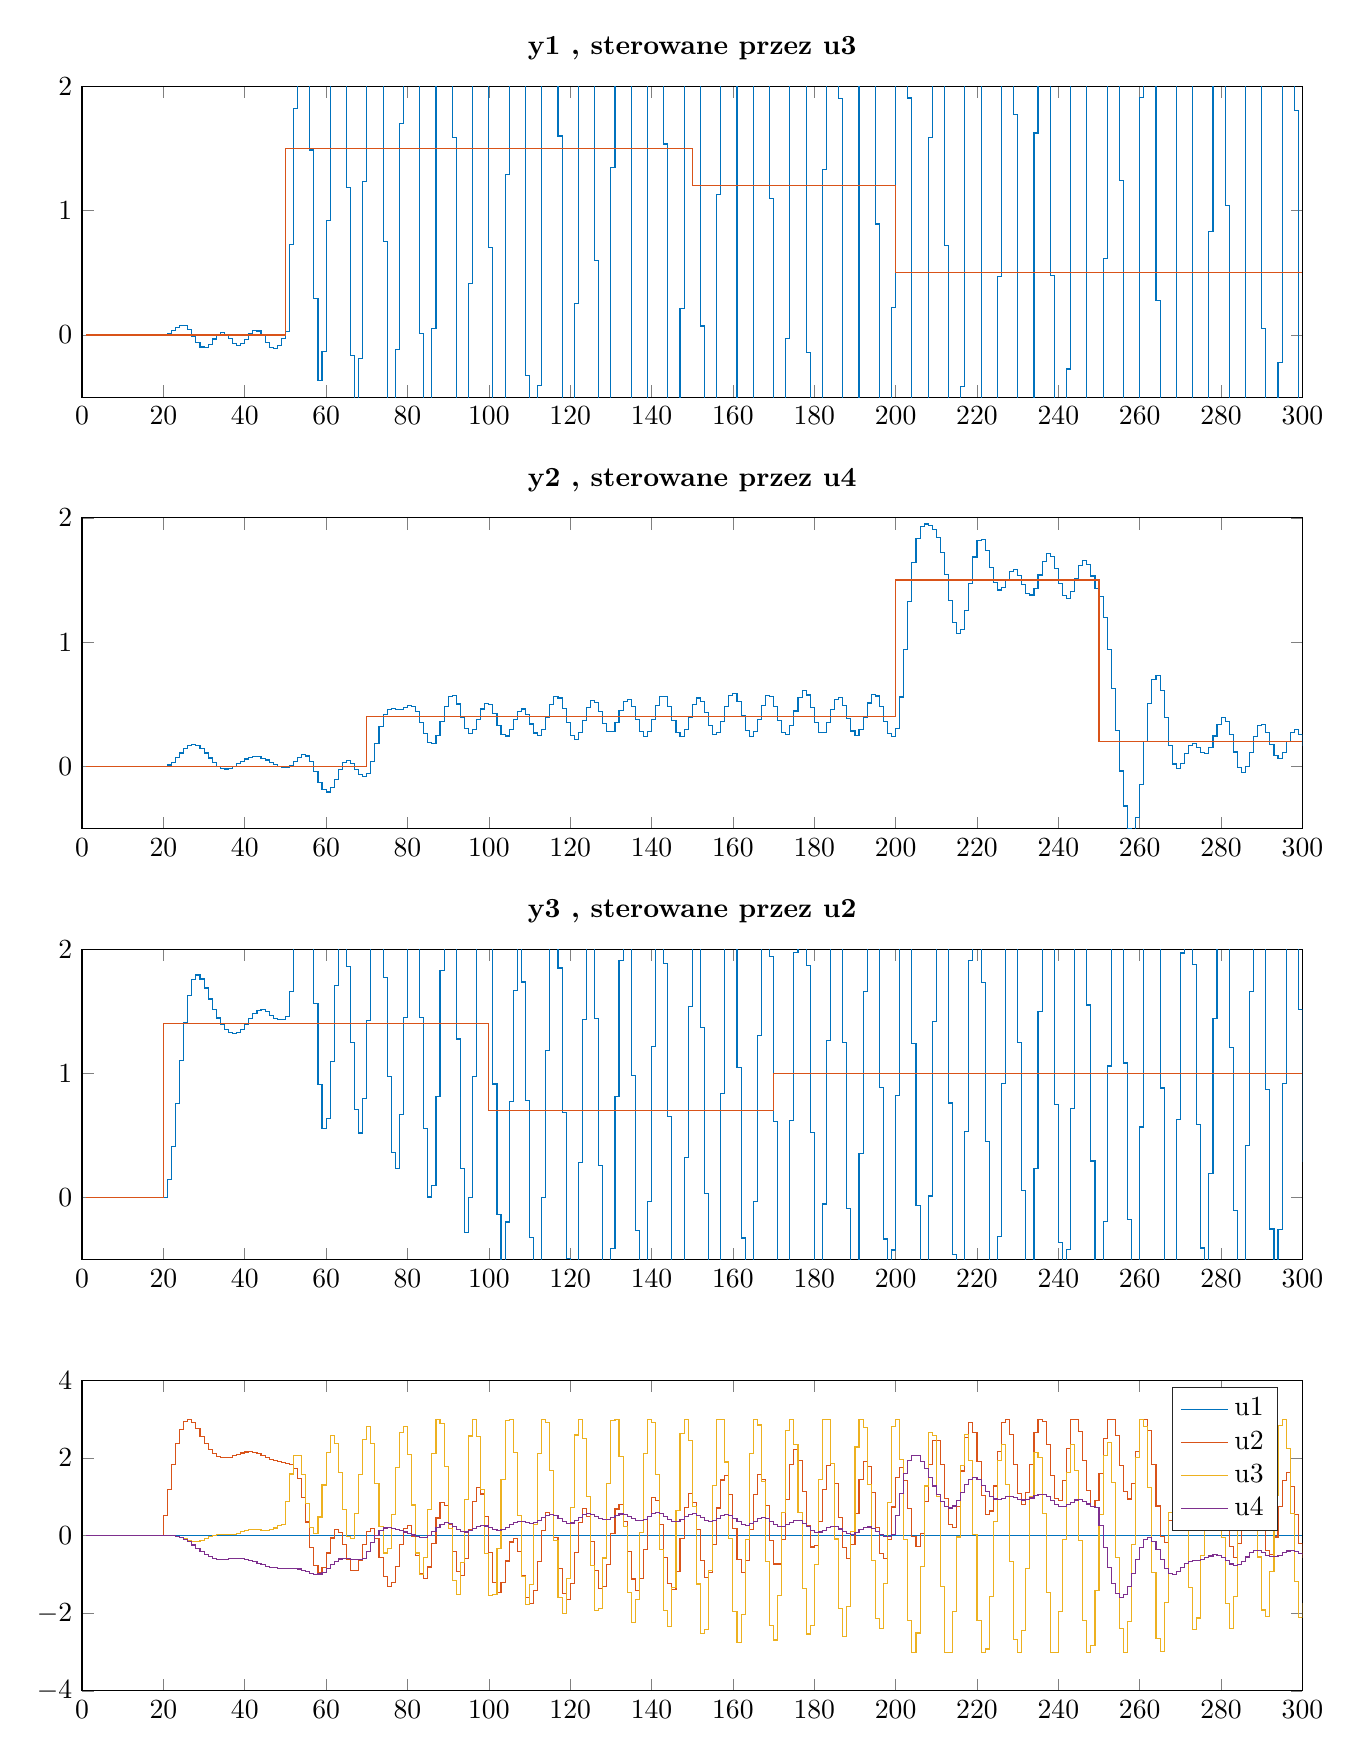
\begin{tikzpicture}

\begin{axis}[%
width=6.102in,
height=1.553in,
at={(1.024in,7.552in)},
scale only axis,
xmin=0,
xmax=300,
ymin=-0.5,
ymax=2,
axis background/.style={fill=white},
title style={font=\bfseries},
title={y1 , sterowane przez u3}
]
\addplot[const plot, color=mycolor1, forget plot] table[row sep=crcr] {%
1	0\\
2	0\\
3	0\\
4	0\\
5	0\\
6	0\\
7	0\\
8	0\\
9	0\\
10	0\\
11	0\\
12	0\\
13	0\\
14	0\\
15	0\\
16	0\\
17	0\\
18	0\\
19	0\\
20	0\\
21	0.0114581194369012\\
22	0.0352462992044872\\
23	0.0626890169702204\\
24	0.0795790972377841\\
25	0.0734520826301614\\
26	0.0405911065210976\\
27	-0.0107878441895741\\
28	-0.0631532178520986\\
29	-0.0971643163931425\\
30	-0.100613713989938\\
31	-0.0744321806441203\\
32	-0.0326249582498168\\
33	0.0041106773346091\\
34	0.0181947362463168\\
35	0.00367798670023886\\
36	-0.0308028521344277\\
37	-0.0662718059958556\\
38	-0.0829557641111786\\
39	-0.0704839109327453\\
40	-0.0336042364652164\\
41	0.0096504444821811\\
42	0.0367076630862104\\
43	0.0319373925164541\\
44	-0.00487052999498487\\
45	-0.0574980108472651\\
46	-0.100626667876022\\
47	-0.112174156173036\\
48	-0.0846161819752689\\
49	-0.0295083738698095\\
50	0.0273998110394422\\
51	0.724997325506459\\
52	1.82426892193668\\
53	2.78738511826281\\
54	3.11369497159876\\
55	2.60787378879939\\
56	1.48870199866991\\
57	0.296882656931718\\
58	-0.364590700310891\\
59	-0.133187567649475\\
60	0.918687504281017\\
61	2.3006677547395\\
62	3.33357268966952\\
63	3.48417050658108\\
64	2.64091161809297\\
65	1.1886394931698\\
66	-0.164271452911435\\
67	-0.729757218841878\\
68	-0.188512188272002\\
69	1.23289174400428\\
70	2.85317119181823\\
71	3.87296025641378\\
72	3.75884424960616\\
73	2.5254872091744\\
74	0.751435709529454\\
75	-0.689068755023632\\
76	-1.05500051107314\\
77	-0.118306133167834\\
78	1.69943117970521\\
79	3.51289193522418\\
80	4.40132874602491\\
81	3.87311656526255\\
82	2.13315882099771\\
83	0.00937857639084949\\
84	-1.43927543209107\\
85	-1.44881569958518\\
86	0.0500838941839432\\
87	2.36639266277243\\
88	4.32358069140648\\
89	4.96420162908475\\
90	3.89903251420345\\
91	1.59074654910639\\
92	-0.849353467080416\\
93	-2.19514645646363\\
94	-1.72026125363021\\
95	0.413020909868026\\
96	3.19725545062013\\
97	4.77732393562461\\
98	4.85786352699644\\
99	3.25438578519223\\
100	0.704061080375279\\
101	-1.54934550761258\\
102	-2.35806809205245\\
103	-1.25329128509323\\
104	1.28812470916881\\
105	4.04368905729408\\
106	5.13375551771725\\
107	4.51907472510833\\
108	2.35722698886186\\
109	-0.323199142652859\\
110	-2.18536676161965\\
111	-2.25128629103057\\
112	-0.409413978994913\\
113	2.49109521740656\\
114	4.64738715203753\\
115	5.38075154511769\\
116	4.19374355812176\\
117	1.60121774742424\\
118	-1.14715486078947\\
119	-2.66997031032563\\
120	-2.144828108502\\
121	0.25128753017619\\
122	3.38800987357241\\
123	5.06760273976848\\
124	5.13139987021018\\
125	3.3706091569996\\
126	0.595770216997279\\
127	-1.83256031473238\\
128	-2.67329377558499\\
129	-1.43402306914089\\
130	1.34728658701357\\
131	4.32976451675554\\
132	5.50097177710786\\
133	4.78841749198711\\
134	2.38559618697228\\
135	-0.566328584377007\\
136	-2.59694648560537\\
137	-2.64026024242452\\
138	-0.588632079963204\\
139	2.61086751526362\\
140	4.88766457356019\\
141	5.63703977962356\\
142	4.33004295185687\\
143	1.537251508319\\
144	-1.39275379017018\\
145	-2.98571568891858\\
146	-2.37900733346594\\
147	0.215363572898669\\
148	3.5713138994334\\
149	5.26876386380948\\
150	5.26161738496985\\
151	3.22091732222259\\
152	0.0724034258396676\\
153	-2.63811754218257\\
154	-3.52125992831826\\
155	-2.05197718020432\\
156	1.12777708200846\\
157	4.38027349861027\\
158	5.60773499825347\\
159	4.75613229285967\\
160	2.0693450329307\\
161	-1.17493142789714\\
162	-3.35978644412138\\
163	-3.3362504517098\\
164	-1.02157466822393\\
165	2.51234142880843\\
166	4.88900366454472\\
167	5.60704093160927\\
168	4.124975652777\\
169	1.09609365882141\\
170	-2.01339254764117\\
171	-3.63342712267818\\
172	-2.87967668305046\\
173	-0.0303755182735664\\
174	3.56395499356227\\
175	5.27424146547299\\
176	5.13839528111768\\
177	3.00373404601512\\
178	-0.139683277114053\\
179	-2.74555690842305\\
180	-3.47601708427362\\
181	-1.88251841656538\\
182	1.32841967686682\\
183	4.38741212889325\\
184	5.52986543899682\\
185	4.60072762180826\\
186	1.90382438590883\\
187	-1.27285836027296\\
188	-3.34216358633429\\
189	-3.21020586463681\\
190	-0.84861606944869\\
191	2.64464004283402\\
192	4.81130757086509\\
193	5.36382721563033\\
194	3.82965074627618\\
195	0.892839821803515\\
196	-2.02074703177204\\
197	-3.43843244324666\\
198	-2.57936281373506\\
199	0.220251947512737\\
200	3.62868473716726\\
201	5.15274709101734\\
202	4.5281291200007\\
203	1.90748843679603\\
204	-1.46028178884362\\
205	-3.62355653971051\\
206	-3.77294082718444\\
207	-1.71380055123305\\
208	1.59169330693018\\
209	4.50909889611725\\
210	5.5338963588411\\
211	4.05796010144586\\
212	0.716557409995745\\
213	-2.56561836713617\\
214	-3.8009243135782\\
215	-3.02083876096188\\
216	-0.411263000191989\\
217	2.79297893482313\\
218	4.99930376872196\\
219	5.05085025787783\\
220	2.82700180137998\\
221	-0.649723450592876\\
222	-2.9098060869345\\
223	-3.66414857102788\\
224	-2.34300653057069\\
225	0.472916052862506\\
226	3.42050845254707\\
227	5.01602041769499\\
228	4.39304314935631\\
229	1.77457256715667\\
230	-1.59933453844453\\
231	-3.26621419626745\\
232	-3.22824618338035\\
233	-1.29993139462258\\
234	1.62590849659584\\
235	4.10963299431335\\
236	4.87277147192531\\
237	3.45624963589009\\
238	0.481228107634314\\
239	-2.48690293787133\\
240	-3.6102855242194\\
241	-2.78937644824838\\
242	-0.273851168008883\\
243	2.73819581559395\\
244	4.74434631216221\\
245	4.68119286961699\\
246	2.49650880607565\\
247	-0.795844745709682\\
248	-3.02100428329543\\
249	-3.65752220528712\\
250	-2.2217897755315\\
251	0.612951291532043\\
252	3.44574702605313\\
253	4.82279646338391\\
254	3.97683010174176\\
255	1.24454146967429\\
256	-2.06226609322432\\
257	-4.12244808941614\\
258	-4.00403271097353\\
259	-1.62942304095902\\
260	1.91111288192089\\
261	4.43243757910525\\
262	5.13589076737498\\
263	3.51401638923313\\
264	0.278948901769219\\
265	-3.00919401069715\\
266	-4.69709958267517\\
267	-3.86652936351855\\
268	-0.830003807266139\\
269	2.97391989900068\\
270	4.55155419513124\\
271	4.30926587507484\\
272	2.11309101057036\\
273	-1.00708163126388\\
274	-3.50675015162303\\
275	-4.0951318480325\\
276	-2.3928870503594\\
277	0.836347504585828\\
278	3.63972277686582\\
279	4.68415422320143\\
280	3.70130076582232\\
281	1.04228655534539\\
282	-2.01986359659811\\
283	-3.95246964956918\\
284	-3.72803993896194\\
285	-1.36448830694649\\
286	2.03800028344604\\
287	3.98224464199378\\
288	4.38720046501745\\
289	2.84587877148775\\
290	0.0527102571426119\\
291	-2.63227927497102\\
292	-3.84899760095082\\
293	-2.92033987695515\\
294	-0.224365617755428\\
295	2.95132628337916\\
296	4.33157694284169\\
297	3.94789757641404\\
298	1.80439032387058\\
299	-1.09093504701813\\
300	-3.30354844445419\\
};
\addplot[const plot, color=mycolor2, forget plot] table[row sep=crcr] {%
1	0\\
2	0\\
3	0\\
4	0\\
5	0\\
6	0\\
7	0\\
8	0\\
9	0\\
10	0\\
11	0\\
12	0\\
13	0\\
14	0\\
15	0\\
16	0\\
17	0\\
18	0\\
19	0\\
20	0\\
21	0\\
22	0\\
23	0\\
24	0\\
25	0\\
26	0\\
27	0\\
28	0\\
29	0\\
30	0\\
31	0\\
32	0\\
33	0\\
34	0\\
35	0\\
36	0\\
37	0\\
38	0\\
39	0\\
40	0\\
41	0\\
42	0\\
43	0\\
44	0\\
45	0\\
46	0\\
47	0\\
48	0\\
49	0\\
50	1.5\\
51	1.5\\
52	1.5\\
53	1.5\\
54	1.5\\
55	1.5\\
56	1.5\\
57	1.5\\
58	1.5\\
59	1.5\\
60	1.5\\
61	1.5\\
62	1.5\\
63	1.5\\
64	1.5\\
65	1.5\\
66	1.5\\
67	1.5\\
68	1.5\\
69	1.5\\
70	1.5\\
71	1.5\\
72	1.5\\
73	1.5\\
74	1.5\\
75	1.5\\
76	1.5\\
77	1.5\\
78	1.5\\
79	1.5\\
80	1.5\\
81	1.5\\
82	1.5\\
83	1.5\\
84	1.5\\
85	1.5\\
86	1.5\\
87	1.5\\
88	1.5\\
89	1.5\\
90	1.5\\
91	1.5\\
92	1.5\\
93	1.5\\
94	1.5\\
95	1.5\\
96	1.5\\
97	1.5\\
98	1.5\\
99	1.5\\
100	1.5\\
101	1.5\\
102	1.5\\
103	1.5\\
104	1.5\\
105	1.5\\
106	1.5\\
107	1.5\\
108	1.5\\
109	1.5\\
110	1.5\\
111	1.5\\
112	1.5\\
113	1.5\\
114	1.5\\
115	1.5\\
116	1.5\\
117	1.5\\
118	1.5\\
119	1.5\\
120	1.5\\
121	1.5\\
122	1.5\\
123	1.5\\
124	1.5\\
125	1.5\\
126	1.5\\
127	1.5\\
128	1.5\\
129	1.5\\
130	1.5\\
131	1.5\\
132	1.5\\
133	1.5\\
134	1.5\\
135	1.5\\
136	1.5\\
137	1.5\\
138	1.5\\
139	1.5\\
140	1.5\\
141	1.5\\
142	1.5\\
143	1.5\\
144	1.5\\
145	1.5\\
146	1.5\\
147	1.5\\
148	1.5\\
149	1.5\\
150	1.2\\
151	1.2\\
152	1.2\\
153	1.2\\
154	1.2\\
155	1.2\\
156	1.2\\
157	1.2\\
158	1.2\\
159	1.2\\
160	1.2\\
161	1.2\\
162	1.2\\
163	1.2\\
164	1.2\\
165	1.2\\
166	1.2\\
167	1.2\\
168	1.2\\
169	1.2\\
170	1.2\\
171	1.2\\
172	1.2\\
173	1.2\\
174	1.2\\
175	1.2\\
176	1.2\\
177	1.2\\
178	1.2\\
179	1.2\\
180	1.2\\
181	1.2\\
182	1.2\\
183	1.2\\
184	1.2\\
185	1.2\\
186	1.2\\
187	1.2\\
188	1.2\\
189	1.2\\
190	1.2\\
191	1.2\\
192	1.2\\
193	1.2\\
194	1.2\\
195	1.2\\
196	1.2\\
197	1.2\\
198	1.2\\
199	1.2\\
200	0.5\\
201	0.5\\
202	0.5\\
203	0.5\\
204	0.5\\
205	0.5\\
206	0.5\\
207	0.5\\
208	0.5\\
209	0.5\\
210	0.5\\
211	0.5\\
212	0.5\\
213	0.5\\
214	0.5\\
215	0.5\\
216	0.5\\
217	0.5\\
218	0.5\\
219	0.5\\
220	0.5\\
221	0.5\\
222	0.5\\
223	0.5\\
224	0.5\\
225	0.5\\
226	0.5\\
227	0.5\\
228	0.5\\
229	0.5\\
230	0.5\\
231	0.5\\
232	0.5\\
233	0.5\\
234	0.5\\
235	0.5\\
236	0.5\\
237	0.5\\
238	0.5\\
239	0.5\\
240	0.5\\
241	0.5\\
242	0.5\\
243	0.5\\
244	0.5\\
245	0.5\\
246	0.5\\
247	0.5\\
248	0.5\\
249	0.5\\
250	0.5\\
251	0.5\\
252	0.5\\
253	0.5\\
254	0.5\\
255	0.5\\
256	0.5\\
257	0.5\\
258	0.5\\
259	0.5\\
260	0.5\\
261	0.5\\
262	0.5\\
263	0.5\\
264	0.5\\
265	0.5\\
266	0.5\\
267	0.5\\
268	0.5\\
269	0.5\\
270	0.5\\
271	0.5\\
272	0.5\\
273	0.5\\
274	0.5\\
275	0.5\\
276	0.5\\
277	0.5\\
278	0.5\\
279	0.5\\
280	0.5\\
281	0.5\\
282	0.5\\
283	0.5\\
284	0.5\\
285	0.5\\
286	0.5\\
287	0.5\\
288	0.5\\
289	0.5\\
290	0.5\\
291	0.5\\
292	0.5\\
293	0.5\\
294	0.5\\
295	0.5\\
296	0.5\\
297	0.5\\
298	0.5\\
299	0.5\\
300	0.5\\
};
\end{axis}

\begin{axis}[%
width=6.102in,
height=1.553in,
at={(1.024in,5.395in)},
scale only axis,
xmin=0,
xmax=300,
ymin=-0.5,
ymax=2,
axis background/.style={fill=white},
title style={font=\bfseries},
title={y2 , sterowane przez u4}
]
\addplot[const plot, color=mycolor1, forget plot] table[row sep=crcr] {%
1	0\\
2	0\\
3	0\\
4	0\\
5	0\\
6	0\\
7	0\\
8	0\\
9	0\\
10	0\\
11	0\\
12	0\\
13	0\\
14	0\\
15	0\\
16	0\\
17	0\\
18	0\\
19	0\\
20	0\\
21	0.0105699306087332\\
22	0.0344208390223349\\
23	0.0689623454117662\\
24	0.10798230645581\\
25	0.143611385060149\\
26	0.16837727915727\\
27	0.177078784224462\\
28	0.167978084869777\\
29	0.14305207518493\\
30	0.107313710160304\\
31	0.0674666590386475\\
32	0.0303154381270715\\
33	0.00137087021266821\\
34	-0.0160292026692769\\
35	-0.0209678249249686\\
36	-0.0146552497537704\\
37	0.000183949575034533\\
38	0.0199992542621832\\
39	0.0410105090924857\\
40	0.0596630333483058\\
41	0.0729852991240023\\
42	0.0789141961364537\\
43	0.0766004140141656\\
44	0.0666216728593955\\
45	0.0509761209444006\\
46	0.032749814559287\\
47	0.0154565096403289\\
48	0.00219233769238188\\
49	-0.005139581287217\\
50	-0.00626386649074016\\
51	0.00810284550530686\\
52	0.0378192910670979\\
53	0.0722591322708968\\
54	0.0933567468428832\\
55	0.0836660644411962\\
56	0.0357188188035246\\
57	-0.0421116031595838\\
58	-0.126823407347093\\
59	-0.189309583519952\\
60	-0.206717936842258\\
61	-0.172958265018898\\
62	-0.102164288104045\\
63	-0.0230437795380142\\
64	0.0336175693084431\\
65	0.0485995858839778\\
66	0.0225624392913204\\
67	-0.02505561346048\\
68	-0.0661496303790671\\
69	-0.0782131129295241\\
70	-0.0557257251746609\\
71	0.0424206888169149\\
72	0.184411445035594\\
73	0.321101106531889\\
74	0.416030801956692\\
75	0.458837593777026\\
76	0.463512497390488\\
77	0.456073228666193\\
78	0.458034263693459\\
79	0.474151383794947\\
80	0.49060679450608\\
81	0.484376723291616\\
82	0.438666255197018\\
83	0.355960998393077\\
84	0.261207230171805\\
85	0.192543861772074\\
86	0.183496510473689\\
87	0.245330925238776\\
88	0.358148513262121\\
89	0.479092204727225\\
90	0.559337667815887\\
91	0.566834956899526\\
92	0.50172068056589\\
93	0.396963207895835\\
94	0.303241863619741\\
95	0.264870048990454\\
96	0.29831090855393\\
97	0.376452146234525\\
98	0.461465501886411\\
99	0.509132839714562\\
100	0.495534015593978\\
101	0.423479008280407\\
102	0.32790169829544\\
103	0.256353701586209\\
104	0.24425736694899\\
105	0.296377741980802\\
106	0.375952508851217\\
107	0.443405320245024\\
108	0.461597542520885\\
109	0.420131899067153\\
110	0.341062979226565\\
111	0.268419964987407\\
112	0.24589450960007\\
113	0.293582083999041\\
114	0.389725570007806\\
115	0.495057479263034\\
116	0.55936761697882\\
117	0.54985396664989\\
118	0.467932016861789\\
119	0.350137475144145\\
120	0.251615568923125\\
121	0.219619847539111\\
122	0.269902107265014\\
123	0.367738463220752\\
124	0.470580302977479\\
125	0.528791276704454\\
126	0.516042750105432\\
127	0.44170942844566\\
128	0.3463251976556\\
129	0.281393904946635\\
130	0.28313726230851\\
131	0.353323651478854\\
132	0.44904540712074\\
133	0.524482656210903\\
134	0.538381422496413\\
135	0.480443090744298\\
136	0.377226142637141\\
137	0.27997153850992\\
138	0.239398699130286\\
139	0.279644526562275\\
140	0.376652631311562\\
141	0.489034381577425\\
142	0.562164283263715\\
143	0.559752092723978\\
144	0.481884830756574\\
145	0.366043056862897\\
146	0.269512935362938\\
147	0.241215697829603\\
148	0.296767545844935\\
149	0.39749141441155\\
150	0.499580835926974\\
151	0.550120508981596\\
152	0.523224137641307\\
153	0.432595984537244\\
154	0.325492272058088\\
155	0.259498672504821\\
156	0.273115851086123\\
157	0.363298413192328\\
158	0.480123024560932\\
159	0.570767520951986\\
160	0.588894105071378\\
161	0.523622026270964\\
162	0.405456522658512\\
163	0.292199884970231\\
164	0.240699894582493\\
165	0.278040311869421\\
166	0.376580961298649\\
167	0.492706204831698\\
168	0.568067562913935\\
169	0.564496379928698\\
170	0.482820768160155\\
171	0.36560239518404\\
172	0.273912414257692\\
173	0.257733527042238\\
174	0.330183029976236\\
175	0.445838606771149\\
176	0.556287762205195\\
177	0.607544525218657\\
178	0.574643973969811\\
179	0.473546153042894\\
180	0.353846212577608\\
181	0.274651269062531\\
182	0.275013718797004\\
183	0.350277272063499\\
184	0.454900656983283\\
185	0.537024889753675\\
186	0.55237503849202\\
187	0.491158353982571\\
188	0.383358283731044\\
189	0.284425971883083\\
190	0.247520744072429\\
191	0.295839222497095\\
192	0.397443447963286\\
193	0.509823447417587\\
194	0.577423542616513\\
195	0.566071603418071\\
196	0.479764487126348\\
197	0.359692879456871\\
198	0.264731835018132\\
199	0.242361429995783\\
200	0.304357781080475\\
201	0.558706351530106\\
202	0.939283785746211\\
203	1.32987598142161\\
204	1.63963591088188\\
205	1.83602449286692\\
206	1.92750496176199\\
207	1.95113230895779\\
208	1.94123767312884\\
209	1.90971414865713\\
210	1.844147759122\\
211	1.72367807651189\\
212	1.5426537028357\\
213	1.33258260823409\\
214	1.15664863307432\\
215	1.06754586610953\\
216	1.10201676287686\\
217	1.25439435351952\\
218	1.47457443886499\\
219	1.68555346017291\\
220	1.81447821893485\\
221	1.82348597597106\\
222	1.73788863915522\\
223	1.60135707918945\\
224	1.47893548903314\\
225	1.4199083292474\\
226	1.43718554358489\\
227	1.50399130343778\\
228	1.56753953258028\\
229	1.58403532292969\\
230	1.53702630622855\\
231	1.46159910824516\\
232	1.39466255127757\\
233	1.37930900147646\\
234	1.43371459319087\\
235	1.54035132447751\\
236	1.6495784095144\\
237	1.71040826017586\\
238	1.6894001863591\\
239	1.59352611163811\\
240	1.47146940200549\\
241	1.37543080817603\\
242	1.35001543795973\\
243	1.40578090337782\\
244	1.51396102255015\\
245	1.61397079015079\\
246	1.65832672147076\\
247	1.62258886352585\\
248	1.53251158324989\\
249	1.42928078260609\\
250	1.36657420522022\\
251	1.19863064505987\\
252	0.939886931706527\\
253	0.626579296349082\\
254	0.290467875448314\\
255	-0.0376130558368502\\
256	-0.319417308522815\\
257	-0.502602050973961\\
258	-0.541646563461359\\
259	-0.414407154873199\\
260	-0.142614442332216\\
261	0.197427807985149\\
262	0.506670212408887\\
263	0.702495601006395\\
264	0.734665335266508\\
265	0.61070370681754\\
266	0.392069922325499\\
267	0.168197080968956\\
268	0.0189066042706525\\
269	-0.0180588527252992\\
270	0.0229361544572908\\
271	0.102880450519948\\
272	0.166725467913291\\
273	0.181874751856721\\
274	0.151636999543033\\
275	0.110211327195949\\
276	0.101252261372481\\
277	0.151080759741288\\
278	0.244767313261069\\
279	0.340533916473986\\
280	0.391768540417849\\
281	0.364417001086216\\
282	0.259491901518863\\
283	0.115748049310945\\
284	-0.00626326455839235\\
285	-0.0522184389983228\\
286	-0.000747186608019645\\
287	0.111599621539188\\
288	0.24037289464195\\
289	0.328162255280941\\
290	0.339197187531181\\
291	0.275087601370363\\
292	0.17342222045407\\
293	0.0888884811363382\\
294	0.0657325460927708\\
295	0.115182381139463\\
296	0.198379307410875\\
297	0.274059798015046\\
298	0.29876602207605\\
299	0.256130524712421\\
300	0.165465515635555\\
};
\addplot[const plot, color=mycolor2, forget plot] table[row sep=crcr] {%
1	0\\
2	0\\
3	0\\
4	0\\
5	0\\
6	0\\
7	0\\
8	0\\
9	0\\
10	0\\
11	0\\
12	0\\
13	0\\
14	0\\
15	0\\
16	0\\
17	0\\
18	0\\
19	0\\
20	0\\
21	0\\
22	0\\
23	0\\
24	0\\
25	0\\
26	0\\
27	0\\
28	0\\
29	0\\
30	0\\
31	0\\
32	0\\
33	0\\
34	0\\
35	0\\
36	0\\
37	0\\
38	0\\
39	0\\
40	0\\
41	0\\
42	0\\
43	0\\
44	0\\
45	0\\
46	0\\
47	0\\
48	0\\
49	0\\
50	0\\
51	0\\
52	0\\
53	0\\
54	0\\
55	0\\
56	0\\
57	0\\
58	0\\
59	0\\
60	0\\
61	0\\
62	0\\
63	0\\
64	0\\
65	0\\
66	0\\
67	0\\
68	0\\
69	0\\
70	0.4\\
71	0.4\\
72	0.4\\
73	0.4\\
74	0.4\\
75	0.4\\
76	0.4\\
77	0.4\\
78	0.4\\
79	0.4\\
80	0.4\\
81	0.4\\
82	0.4\\
83	0.4\\
84	0.4\\
85	0.4\\
86	0.4\\
87	0.4\\
88	0.4\\
89	0.4\\
90	0.4\\
91	0.4\\
92	0.4\\
93	0.4\\
94	0.4\\
95	0.4\\
96	0.4\\
97	0.4\\
98	0.4\\
99	0.4\\
100	0.4\\
101	0.4\\
102	0.4\\
103	0.4\\
104	0.4\\
105	0.4\\
106	0.4\\
107	0.4\\
108	0.4\\
109	0.4\\
110	0.4\\
111	0.4\\
112	0.4\\
113	0.4\\
114	0.4\\
115	0.4\\
116	0.4\\
117	0.4\\
118	0.4\\
119	0.4\\
120	0.4\\
121	0.4\\
122	0.4\\
123	0.4\\
124	0.4\\
125	0.4\\
126	0.4\\
127	0.4\\
128	0.4\\
129	0.4\\
130	0.4\\
131	0.4\\
132	0.4\\
133	0.4\\
134	0.4\\
135	0.4\\
136	0.4\\
137	0.4\\
138	0.4\\
139	0.4\\
140	0.4\\
141	0.4\\
142	0.4\\
143	0.4\\
144	0.4\\
145	0.4\\
146	0.4\\
147	0.4\\
148	0.4\\
149	0.4\\
150	0.4\\
151	0.4\\
152	0.4\\
153	0.4\\
154	0.4\\
155	0.4\\
156	0.4\\
157	0.4\\
158	0.4\\
159	0.4\\
160	0.4\\
161	0.4\\
162	0.4\\
163	0.4\\
164	0.4\\
165	0.4\\
166	0.4\\
167	0.4\\
168	0.4\\
169	0.4\\
170	0.4\\
171	0.4\\
172	0.4\\
173	0.4\\
174	0.4\\
175	0.4\\
176	0.4\\
177	0.4\\
178	0.4\\
179	0.4\\
180	0.4\\
181	0.4\\
182	0.4\\
183	0.4\\
184	0.4\\
185	0.4\\
186	0.4\\
187	0.4\\
188	0.4\\
189	0.4\\
190	0.4\\
191	0.4\\
192	0.4\\
193	0.4\\
194	0.4\\
195	0.4\\
196	0.4\\
197	0.4\\
198	0.4\\
199	0.4\\
200	1.5\\
201	1.5\\
202	1.5\\
203	1.5\\
204	1.5\\
205	1.5\\
206	1.5\\
207	1.5\\
208	1.5\\
209	1.5\\
210	1.5\\
211	1.5\\
212	1.5\\
213	1.5\\
214	1.5\\
215	1.5\\
216	1.5\\
217	1.5\\
218	1.5\\
219	1.5\\
220	1.5\\
221	1.5\\
222	1.5\\
223	1.5\\
224	1.5\\
225	1.5\\
226	1.5\\
227	1.5\\
228	1.5\\
229	1.5\\
230	1.5\\
231	1.5\\
232	1.5\\
233	1.5\\
234	1.5\\
235	1.5\\
236	1.5\\
237	1.5\\
238	1.5\\
239	1.5\\
240	1.5\\
241	1.5\\
242	1.5\\
243	1.5\\
244	1.5\\
245	1.5\\
246	1.5\\
247	1.5\\
248	1.5\\
249	1.5\\
250	0.2\\
251	0.2\\
252	0.2\\
253	0.2\\
254	0.2\\
255	0.2\\
256	0.2\\
257	0.2\\
258	0.2\\
259	0.2\\
260	0.2\\
261	0.2\\
262	0.2\\
263	0.2\\
264	0.2\\
265	0.2\\
266	0.2\\
267	0.2\\
268	0.2\\
269	0.2\\
270	0.2\\
271	0.2\\
272	0.2\\
273	0.2\\
274	0.2\\
275	0.2\\
276	0.2\\
277	0.2\\
278	0.2\\
279	0.2\\
280	0.2\\
281	0.2\\
282	0.2\\
283	0.2\\
284	0.2\\
285	0.2\\
286	0.2\\
287	0.2\\
288	0.2\\
289	0.2\\
290	0.2\\
291	0.2\\
292	0.2\\
293	0.2\\
294	0.2\\
295	0.2\\
296	0.2\\
297	0.2\\
298	0.2\\
299	0.2\\
300	0.2\\
};
\end{axis}

\begin{axis}[%
width=6.102in,
height=1.553in,
at={(1.024in,3.239in)},
scale only axis,
xmin=0,
xmax=300,
ymin=-0.5,
ymax=2,
axis background/.style={fill=white},
title style={font=\bfseries},
title={y3 , sterowane przez u2}
]
\addplot[const plot, color=mycolor1, forget plot] table[row sep=crcr] {%
1	0\\
2	0\\
3	0\\
4	0\\
5	0\\
6	0\\
7	0\\
8	0\\
9	0\\
10	0\\
11	0\\
12	0\\
13	0\\
14	0\\
15	0\\
16	0\\
17	0\\
18	0\\
19	0\\
20	0\\
21	0.142671982788199\\
22	0.414294892302412\\
23	0.755746235167961\\
24	1.10354718616354\\
25	1.40558833073036\\
26	1.62705297893935\\
27	1.75372232620367\\
28	1.79112934989601\\
29	1.75960119605521\\
30	1.6865628937674\\
31	1.59844122226234\\
32	1.51464526786508\\
33	1.44525421242351\\
34	1.392527185943\\
35	1.35481907293157\\
36	1.33063280262062\\
37	1.32075636876188\\
38	1.32761070771687\\
39	1.35249414497591\\
40	1.39257542761563\\
41	1.43966820200113\\
42	1.48190732849198\\
43	1.50788732273848\\
44	1.51140742654173\\
45	1.49444448980081\\
46	1.46666519557452\\
47	1.44140540038441\\
48	1.42980937630099\\
49	1.43584263194734\\
50	1.45460912221585\\
51	1.65903920888981\\
52	2.05124350085895\\
53	2.49004512537083\\
54	2.7613606339081\\
55	2.69112522095471\\
56	2.24491520305016\\
57	1.56338463590178\\
58	0.910074992288028\\
59	0.552690578755781\\
60	0.634129400336735\\
61	1.09780201240885\\
62	1.70764989340747\\
63	2.15750862479411\\
64	2.2192365979734\\
65	1.85725095111164\\
66	1.25084420152847\\
67	0.709542689577619\\
68	0.519977676469841\\
69	0.798813580609479\\
70	1.42626234429215\\
71	2.10274823221237\\
72	2.48583703822486\\
73	2.36406754335111\\
74	1.77005019762605\\
75	0.974616444540864\\
76	0.360325978906114\\
77	0.233355046358274\\
78	0.666223612706056\\
79	1.45213186112472\\
80	2.19864956020221\\
81	2.51919673338511\\
82	2.22951597652612\\
83	1.44985109454001\\
84	0.557018175781543\\
85	0.00414719180066747\\
86	0.0936552322441612\\
87	0.816438699090428\\
88	1.83030890241583\\
89	2.64907418259197\\
90	2.85400887087324\\
91	2.31689803968361\\
92	1.27670735388257\\
93	0.235160206549042\\
94	-0.28470226742542\\
95	-0.0011889455946793\\
96	0.973925970713611\\
97	2.04416042463675\\
98	2.77140125956616\\
99	2.78625635495067\\
100	2.07446315839019\\
101	0.91426416330278\\
102	-0.138198021174483\\
103	-0.573902099538054\\
104	-0.196737725474405\\
105	0.772942238272176\\
106	1.66641236033016\\
107	2.0735409847944\\
108	1.73477332504596\\
109	0.783134072230663\\
110	-0.320210017320722\\
111	-1.01004487410402\\
112	-0.902133531418911\\
113	0.000924063786366391\\
114	1.18625491360521\\
115	2.15657784056249\\
116	2.42684701391749\\
117	1.84806826240763\\
118	0.68741167614373\\
119	-0.489623075759842\\
120	-1.09080273701928\\
121	-0.793805657456399\\
122	0.281008762219099\\
123	1.43615235344433\\
124	2.21704515370296\\
125	2.22231235170769\\
126	1.44085209538173\\
127	0.256124240554265\\
128	-0.734556072382447\\
129	-1.01325897187338\\
130	-0.406595292090823\\
131	0.812883716350792\\
132	1.90553496822146\\
133	2.41062467802288\\
134	2.0505639850683\\
135	0.985072285630978\\
136	-0.264224189502457\\
137	-1.06436139513698\\
138	-0.986367164697026\\
139	-0.0308943132905666\\
140	1.21553493279174\\
141	2.2353255144883\\
142	2.5097316108444\\
143	1.88454845719716\\
144	0.650538597274848\\
145	-0.58650666857118\\
146	-1.19810966550896\\
147	-0.84931796536191\\
148	0.320341438499352\\
149	1.53939226753256\\
150	2.34459597183365\\
151	2.28691237786039\\
152	1.36791431402107\\
153	0.0302998672396532\\
154	-1.05205746968839\\
155	-1.30659146229153\\
156	-0.557440825452837\\
157	0.839230187149354\\
158	2.07162031699262\\
159	2.63308224041827\\
160	2.22838935617712\\
161	1.04753496711218\\
162	-0.325229390387083\\
163	-1.1921458570281\\
164	-1.0891503037555\\
165	-0.0294173532468754\\
166	1.30725450014339\\
167	2.38072269350797\\
168	2.64214334066381\\
169	1.94367775495333\\
170	0.613564540598289\\
171	-0.661667123240797\\
172	-1.21868139785715\\
173	-0.729612931873013\\
174	0.621540275653009\\
175	1.9749771322884\\
176	2.8399955142037\\
177	2.79321031504088\\
178	1.86652946878184\\
179	0.526826471977994\\
180	-0.545365171273206\\
181	-0.789616643196305\\
182	-0.0519851495414265\\
183	1.26359433218567\\
184	2.41538901829115\\
185	2.89656281667322\\
186	2.43889454550247\\
187	1.2489476894695\\
188	-0.0891641247851584\\
189	-0.895323238568667\\
190	-0.733566179351177\\
191	0.356880437801395\\
192	1.65700817890177\\
193	2.66756340181713\\
194	2.87678100673849\\
195	2.17081687677103\\
196	0.888574774047812\\
197	-0.333480408317582\\
198	-0.869868175716521\\
199	-0.421952703341107\\
200	0.818653712438546\\
201	2.03470202534451\\
202	2.66956626316626\\
203	2.36216940283713\\
204	1.24017340704812\\
205	-0.0663563946859501\\
206	-0.943884064919926\\
207	-0.924223090130792\\
208	0.0127216673143004\\
209	1.41775720883025\\
210	2.58355148787922\\
211	2.89513784978724\\
212	2.14867469110244\\
213	0.761498321549473\\
214	-0.460721780335836\\
215	-1.02935302491974\\
216	-0.640210357985701\\
217	0.530071140942968\\
218	1.91031479100737\\
219	2.80744903935438\\
220	2.74940417545189\\
221	1.73113171740735\\
222	0.447946233833714\\
223	-0.614818902886296\\
224	-0.921759633428718\\
225	-0.313509009560002\\
226	0.918329775934083\\
227	2.16378476750766\\
228	2.75684791732262\\
229	2.40508677947356\\
230	1.24613261309268\\
231	0.0599021746649381\\
232	-0.702738450184386\\
233	-0.63923411931288\\
234	0.235550088417701\\
235	1.4988261062819\\
236	2.47999916213734\\
237	2.70338056310855\\
238	2.01047685011304\\
239	0.746556234356587\\
240	-0.359429671490216\\
241	-0.834595382143109\\
242	-0.414944587504802\\
243	0.714028595565377\\
244	2.00426983877719\\
245	2.72683571030258\\
246	2.56956233502353\\
247	1.55007493518016\\
248	0.294098791509764\\
249	-0.685287028651993\\
250	-0.883019636750597\\
251	-0.193023514840352\\
252	1.05922010624444\\
253	2.20940130871938\\
254	2.68198902913383\\
255	2.24442056020691\\
256	1.08299042537526\\
257	-0.17516300060937\\
258	-0.887411202301119\\
259	-0.62336155710945\\
260	0.567888345531154\\
261	2.03355479651101\\
262	3.05760697547108\\
263	3.2181697830037\\
264	2.37178754633523\\
265	0.881877315593369\\
266	-0.54760066821756\\
267	-1.2111046719364\\
268	-0.755723976348223\\
269	0.626860703585856\\
270	1.96859675417394\\
271	2.82446967470534\\
272	2.77772587780249\\
273	1.87544338787703\\
274	0.590949628210743\\
275	-0.405561823037386\\
276	-0.579099139475455\\
277	0.194093824965652\\
278	1.44316155565361\\
279	2.51702740633409\\
280	2.91593649048476\\
281	2.4043231147625\\
282	1.20461838518644\\
283	-0.104429183827377\\
284	-0.865538682562025\\
285	-0.671481607574626\\
286	0.418371870201548\\
287	1.66056543136701\\
288	2.60199069575965\\
289	2.77045228784126\\
290	2.0807561706925\\
291	0.87135094909944\\
292	-0.252893436327919\\
293	-0.714768572379644\\
294	-0.256632258237432\\
295	0.917881740986997\\
296	2.03926760299375\\
297	2.66547957312143\\
298	2.46047683031351\\
299	1.51116463740722\\
300	0.283127106450758\\
};
\addplot[const plot, color=mycolor2, forget plot] table[row sep=crcr] {%
1	0\\
2	0\\
3	0\\
4	0\\
5	0\\
6	0\\
7	0\\
8	0\\
9	0\\
10	0\\
11	0\\
12	0\\
13	0\\
14	0\\
15	0\\
16	0\\
17	0\\
18	0\\
19	0\\
20	1.4\\
21	1.4\\
22	1.4\\
23	1.4\\
24	1.4\\
25	1.4\\
26	1.4\\
27	1.4\\
28	1.4\\
29	1.4\\
30	1.4\\
31	1.4\\
32	1.4\\
33	1.4\\
34	1.4\\
35	1.4\\
36	1.4\\
37	1.4\\
38	1.4\\
39	1.4\\
40	1.4\\
41	1.4\\
42	1.4\\
43	1.4\\
44	1.4\\
45	1.4\\
46	1.4\\
47	1.4\\
48	1.4\\
49	1.4\\
50	1.4\\
51	1.4\\
52	1.4\\
53	1.4\\
54	1.4\\
55	1.4\\
56	1.4\\
57	1.4\\
58	1.4\\
59	1.4\\
60	1.4\\
61	1.4\\
62	1.4\\
63	1.4\\
64	1.4\\
65	1.4\\
66	1.4\\
67	1.4\\
68	1.4\\
69	1.4\\
70	1.4\\
71	1.4\\
72	1.4\\
73	1.4\\
74	1.4\\
75	1.4\\
76	1.4\\
77	1.4\\
78	1.4\\
79	1.4\\
80	1.4\\
81	1.4\\
82	1.4\\
83	1.4\\
84	1.4\\
85	1.4\\
86	1.4\\
87	1.4\\
88	1.4\\
89	1.4\\
90	1.4\\
91	1.4\\
92	1.4\\
93	1.4\\
94	1.4\\
95	1.4\\
96	1.4\\
97	1.4\\
98	1.4\\
99	1.4\\
100	0.7\\
101	0.7\\
102	0.7\\
103	0.7\\
104	0.7\\
105	0.7\\
106	0.7\\
107	0.7\\
108	0.7\\
109	0.7\\
110	0.7\\
111	0.7\\
112	0.7\\
113	0.7\\
114	0.7\\
115	0.7\\
116	0.7\\
117	0.7\\
118	0.7\\
119	0.7\\
120	0.7\\
121	0.7\\
122	0.7\\
123	0.7\\
124	0.7\\
125	0.7\\
126	0.7\\
127	0.7\\
128	0.7\\
129	0.7\\
130	0.7\\
131	0.7\\
132	0.7\\
133	0.7\\
134	0.7\\
135	0.7\\
136	0.7\\
137	0.7\\
138	0.7\\
139	0.7\\
140	0.7\\
141	0.7\\
142	0.7\\
143	0.7\\
144	0.7\\
145	0.7\\
146	0.7\\
147	0.7\\
148	0.7\\
149	0.7\\
150	0.7\\
151	0.7\\
152	0.7\\
153	0.7\\
154	0.7\\
155	0.7\\
156	0.7\\
157	0.7\\
158	0.7\\
159	0.7\\
160	0.7\\
161	0.7\\
162	0.7\\
163	0.7\\
164	0.7\\
165	0.7\\
166	0.7\\
167	0.7\\
168	0.7\\
169	0.7\\
170	1\\
171	1\\
172	1\\
173	1\\
174	1\\
175	1\\
176	1\\
177	1\\
178	1\\
179	1\\
180	1\\
181	1\\
182	1\\
183	1\\
184	1\\
185	1\\
186	1\\
187	1\\
188	1\\
189	1\\
190	1\\
191	1\\
192	1\\
193	1\\
194	1\\
195	1\\
196	1\\
197	1\\
198	1\\
199	1\\
200	1\\
201	1\\
202	1\\
203	1\\
204	1\\
205	1\\
206	1\\
207	1\\
208	1\\
209	1\\
210	1\\
211	1\\
212	1\\
213	1\\
214	1\\
215	1\\
216	1\\
217	1\\
218	1\\
219	1\\
220	1\\
221	1\\
222	1\\
223	1\\
224	1\\
225	1\\
226	1\\
227	1\\
228	1\\
229	1\\
230	1\\
231	1\\
232	1\\
233	1\\
234	1\\
235	1\\
236	1\\
237	1\\
238	1\\
239	1\\
240	1\\
241	1\\
242	1\\
243	1\\
244	1\\
245	1\\
246	1\\
247	1\\
248	1\\
249	1\\
250	1\\
251	1\\
252	1\\
253	1\\
254	1\\
255	1\\
256	1\\
257	1\\
258	1\\
259	1\\
260	1\\
261	1\\
262	1\\
263	1\\
264	1\\
265	1\\
266	1\\
267	1\\
268	1\\
269	1\\
270	1\\
271	1\\
272	1\\
273	1\\
274	1\\
275	1\\
276	1\\
277	1\\
278	1\\
279	1\\
280	1\\
281	1\\
282	1\\
283	1\\
284	1\\
285	1\\
286	1\\
287	1\\
288	1\\
289	1\\
290	1\\
291	1\\
292	1\\
293	1\\
294	1\\
295	1\\
296	1\\
297	1\\
298	1\\
299	1\\
300	1\\
};
\end{axis}

\begin{axis}[%
width=6.102in,
height=1.553in,
at={(1.024in,1.083in)},
scale only axis,
xmin=0,
xmax=300,
ymin=-4,
ymax=4,
axis background/.style={fill=white},
legend style={legend cell align=left, align=left, draw=white!15!black}
]
\addplot[const plot, color=mycolor1] table[row sep=crcr] {%
1	0\\
2	0\\
3	0\\
4	0\\
5	0\\
6	0\\
7	0\\
8	0\\
9	0\\
10	0\\
11	0\\
12	0\\
13	0\\
14	0\\
15	0\\
16	0\\
17	0\\
18	0\\
19	0\\
20	0\\
21	0\\
22	0\\
23	0\\
24	0\\
25	0\\
26	0\\
27	0\\
28	0\\
29	0\\
30	0\\
31	0\\
32	0\\
33	0\\
34	0\\
35	0\\
36	0\\
37	0\\
38	0\\
39	0\\
40	0\\
41	0\\
42	0\\
43	0\\
44	0\\
45	0\\
46	0\\
47	0\\
48	0\\
49	0\\
50	0\\
51	0\\
52	0\\
53	0\\
54	0\\
55	0\\
56	0\\
57	0\\
58	0\\
59	0\\
60	0\\
61	0\\
62	0\\
63	0\\
64	0\\
65	0\\
66	0\\
67	0\\
68	0\\
69	0\\
70	0\\
71	0\\
72	0\\
73	0\\
74	0\\
75	0\\
76	0\\
77	0\\
78	0\\
79	0\\
80	0\\
81	0\\
82	0\\
83	0\\
84	0\\
85	0\\
86	0\\
87	0\\
88	0\\
89	0\\
90	0\\
91	0\\
92	0\\
93	0\\
94	0\\
95	0\\
96	0\\
97	0\\
98	0\\
99	0\\
100	0\\
101	0\\
102	0\\
103	0\\
104	0\\
105	0\\
106	0\\
107	0\\
108	0\\
109	0\\
110	0\\
111	0\\
112	0\\
113	0\\
114	0\\
115	0\\
116	0\\
117	0\\
118	0\\
119	0\\
120	0\\
121	0\\
122	0\\
123	0\\
124	0\\
125	0\\
126	0\\
127	0\\
128	0\\
129	0\\
130	0\\
131	0\\
132	0\\
133	0\\
134	0\\
135	0\\
136	0\\
137	0\\
138	0\\
139	0\\
140	0\\
141	0\\
142	0\\
143	0\\
144	0\\
145	0\\
146	0\\
147	0\\
148	0\\
149	0\\
150	0\\
151	0\\
152	0\\
153	0\\
154	0\\
155	0\\
156	0\\
157	0\\
158	0\\
159	0\\
160	0\\
161	0\\
162	0\\
163	0\\
164	0\\
165	0\\
166	0\\
167	0\\
168	0\\
169	0\\
170	0\\
171	0\\
172	0\\
173	0\\
174	0\\
175	0\\
176	0\\
177	0\\
178	0\\
179	0\\
180	0\\
181	0\\
182	0\\
183	0\\
184	0\\
185	0\\
186	0\\
187	0\\
188	0\\
189	0\\
190	0\\
191	0\\
192	0\\
193	0\\
194	0\\
195	0\\
196	0\\
197	0\\
198	0\\
199	0\\
200	0\\
201	0\\
202	0\\
203	0\\
204	0\\
205	0\\
206	0\\
207	0\\
208	0\\
209	0\\
210	0\\
211	0\\
212	0\\
213	0\\
214	0\\
215	0\\
216	0\\
217	0\\
218	0\\
219	0\\
220	0\\
221	0\\
222	0\\
223	0\\
224	0\\
225	0\\
226	0\\
227	0\\
228	0\\
229	0\\
230	0\\
231	0\\
232	0\\
233	0\\
234	0\\
235	0\\
236	0\\
237	0\\
238	0\\
239	0\\
240	0\\
241	0\\
242	0\\
243	0\\
244	0\\
245	0\\
246	0\\
247	0\\
248	0\\
249	0\\
250	0\\
251	0\\
252	0\\
253	0\\
254	0\\
255	0\\
256	0\\
257	0\\
258	0\\
259	0\\
260	0\\
261	0\\
262	0\\
263	0\\
264	0\\
265	0\\
266	0\\
267	0\\
268	0\\
269	0\\
270	0\\
271	0\\
272	0\\
273	0\\
274	0\\
275	0\\
276	0\\
277	0\\
278	0\\
279	0\\
280	0\\
281	0\\
282	0\\
283	0\\
284	0\\
285	0\\
286	0\\
287	0\\
288	0\\
289	0\\
290	0\\
291	0\\
292	0\\
293	0\\
294	0\\
295	0\\
296	0\\
297	0\\
298	0\\
299	0\\
300	0\\
};
\addlegendentry{u1}

\addplot[const plot, color=mycolor2] table[row sep=crcr] {%
1	0\\
2	0\\
3	0\\
4	0\\
5	0\\
6	0\\
7	0\\
8	0\\
9	0\\
10	0\\
11	0\\
12	0\\
13	0\\
14	0\\
15	0\\
16	0\\
17	0\\
18	0\\
19	0\\
20	0.518\\
21	1.19\\
22	1.83721136636837\\
23	2.36822833810977\\
24	2.7401763532886\\
25	2.94044591069356\\
26	2.98387311314198\\
27	2.90517785083081\\
28	2.74921299583752\\
29	2.5610446209148\\
30	2.37789350336174\\
31	2.22448651410381\\
32	2.11234931963122\\
33	2.04237077819694\\
34	2.00904691568984\\
35	2.00454098816704\\
36	2.02117485648016\\
37	2.05196007776919\\
38	2.0898142315804\\
39	2.12670241310893\\
40	2.15382727424375\\
41	2.16324779592428\\
42	2.15033738124663\\
43	2.11581665893216\\
44	2.06609517934478\\
45	2.01136867945327\\
46	1.96201165485261\\
47	1.92472849008111\\
48	1.90018643062967\\
49	1.88326906344453\\
50	1.86590015022322\\
51	1.84115589796313\\
52	1.73858753459121\\
53	1.4680409438512\\
54	0.987906678191711\\
55	0.351273409837741\\
56	-0.29799349415281\\
57	-0.779863106264549\\
58	-0.959078598302818\\
59	-0.812676959459587\\
60	-0.448548415468945\\
61	-0.0621737571024332\\
62	0.150831452694135\\
63	0.0855601827616632\\
64	-0.222515536935157\\
65	-0.615112024780817\\
66	-0.88956107496508\\
67	-0.901055766112362\\
68	-0.638324442446445\\
69	-0.233782762624394\\
70	0.0992678143468641\\
71	0.173281699562329\\
72	-0.0776002758405731\\
73	-0.557187532412974\\
74	-1.04738956230187\\
75	-1.31207230595662\\
76	-1.21466726304263\\
77	-0.790596688089909\\
78	-0.23606624181296\\
79	0.184555446808267\\
80	0.26931495986729\\
81	-0.0172443543853669\\
82	-0.520241234582596\\
83	-0.966246777773667\\
84	-1.09832237483905\\
85	-0.808493039808142\\
86	-0.200296522001159\\
87	0.453454487454798\\
88	0.840987149408468\\
89	0.772091493969781\\
90	0.274271293163201\\
91	-0.40971632719333\\
92	-0.933891061324162\\
93	-1.01821174404337\\
94	-0.591996790187273\\
95	0.161941278962086\\
96	0.888995234117933\\
97	1.23446745431782\\
98	1.07102001933562\\
99	0.501265387171824\\
100	-0.434386811204937\\
101	-1.19985440404521\\
102	-1.47204821898917\\
103	-1.21297327228572\\
104	-0.653712996393503\\
105	-0.165026846595297\\
106	-0.0678962829630569\\
107	-0.415557747985666\\
108	-1.03153211676136\\
109	-1.58481600256235\\
110	-1.75687149473864\\
111	-1.40923400277626\\
112	-0.665956978897108\\
113	0.135341564225746\\
114	0.604435246562951\\
115	0.5334619521409\\
116	-0.0449783706395235\\
117	-0.853860426522974\\
118	-1.49773041195597\\
119	-1.65389718127234\\
120	-1.23531329286516\\
121	-0.44160597535732\\
122	0.331882880488866\\
123	0.687044315528389\\
124	0.490633094059016\\
125	-0.143270546934336\\
126	-0.888124131042394\\
127	-1.36003466809554\\
128	-1.30774061462676\\
129	-0.742945576213862\\
130	0.0576389265302703\\
131	0.684228792957595\\
132	0.79845247947526\\
133	0.362119238276547\\
134	-0.405678413423295\\
135	-1.11766650184551\\
136	-1.40591777944695\\
137	-1.10752406045181\\
138	-0.354347129118479\\
139	0.482972959074537\\
140	0.974191471011459\\
141	0.89756926363442\\
142	0.287407866932469\\
143	-0.561389334329507\\
144	-1.22944925097511\\
145	-1.37764349447537\\
146	-0.919886241948215\\
147	-0.0750807041125654\\
148	0.732689139648751\\
149	1.08154997690398\\
150	0.843723638989244\\
151	0.150483151212227\\
152	-0.63436783084847\\
153	-1.08894840803758\\
154	-0.946368181015781\\
155	-0.23779818890786\\
156	0.710760976460935\\
157	1.43178029212432\\
158	1.5587154429247\\
159	1.06104942156006\\
160	0.192146153993126\\
161	-0.613429360578273\\
162	-0.948801772397628\\
163	-0.63826353146029\\
164	0.167654969240443\\
165	1.05828121371081\\
166	1.56281508496582\\
167	1.45414983484503\\
168	0.780072790296245\\
169	-0.13554483203811\\
170	-0.73195582271402\\
171	-0.731622122593529\\
172	-0.0931709415593119\\
173	0.918253268392357\\
174	1.83549834941447\\
175	2.21015949788604\\
176	1.92564078725496\\
177	1.1451641569348\\
178	0.259777291161502\\
179	-0.294891657226349\\
180	-0.250999899725027\\
181	0.355503712352844\\
182	1.19711550973597\\
183	1.81411514924336\\
184	1.86809594564814\\
185	1.33644633533082\\
186	0.47375341450599\\
187	-0.295567257529802\\
188	-0.583887558972254\\
189	-0.23705896955344\\
190	0.579039728653945\\
191	1.45072805375214\\
192	1.91728103626562\\
193	1.77960248550084\\
194	1.10319551839328\\
195	0.212214408122118\\
196	-0.46078501506074\\
197	-0.585883158038013\\
198	-0.103654969641188\\
199	0.737107604807903\\
200	1.49558521253928\\
201	1.75649549981887\\
202	1.42204289613998\\
203	0.694113081731799\\
204	-0.014235926773119\\
205	-0.286330046956334\\
206	0.054559356245431\\
207	0.886292195540296\\
208	1.8334091139236\\
209	2.44924431823009\\
210	2.44175922936095\\
211	1.82963745252802\\
212	0.945890640263426\\
213	0.280744811321342\\
214	0.204733459331023\\
215	0.748462208862791\\
216	1.66477225748905\\
217	2.52409335829164\\
218	2.91897723601957\\
219	2.66665714500283\\
220	1.90716495061204\\
221	1.04285971554571\\
222	0.543757540018191\\
223	0.63260486107587\\
224	1.27619113507394\\
225	2.17591335408339\\
226	2.90560162535547\\
227	3\\
228	2.60465354086062\\
229	1.82823689150672\\
230	1.09182581684586\\
231	0.811060245913026\\
232	1.10372011825733\\
233	1.83222145335056\\
234	2.64484126352331\\
235	3\\
236	2.93230851333601\\
237	2.34512694988583\\
238	1.54209971157492\\
239	0.951251431848402\\
240	0.899805560361858\\
241	1.41046381603175\\
242	2.2438702466015\\
243	2.99639382944382\\
244	3\\
245	2.68817590589035\\
246	1.94449643890159\\
247	1.15372105003406\\
248	0.74300475295876\\
249	0.912288710529859\\
250	1.60249254536142\\
251	2.49870940828066\\
252	3\\
253	3\\
254	2.56986777438375\\
255	1.81331328752021\\
256	1.14367086086455\\
257	0.942438361270264\\
258	1.34323131350031\\
259	2.16918157991125\\
260	3\\
261	3\\
262	2.69758423842469\\
263	1.83122086297355\\
264	0.763490180030147\\
265	-0.0292220277537177\\
266	-0.180776660280214\\
267	0.377393331318308\\
268	1.36810058712684\\
269	2.29189198565304\\
270	2.66730525616331\\
271	2.38508425925147\\
272	1.61094762257964\\
273	0.733125448491655\\
274	0.177172154924774\\
275	0.196667502264276\\
276	0.744212049927386\\
277	1.4912715395032\\
278	1.99126896606896\\
279	1.94753085252041\\
280	1.35360106455559\\
281	0.468968317266405\\
282	-0.291724797275726\\
283	-0.560227872228279\\
284	-0.202183558877907\\
285	0.605460596187325\\
286	1.45120662974831\\
287	1.88758278825818\\
288	1.74058230508171\\
289	1.08681611279624\\
290	0.242318481134072\\
291	-0.384350867599886\\
292	-0.491042943299679\\
293	-0.0349360996731373\\
294	0.739919531121413\\
295	1.41855587835758\\
296	1.6214645540461\\
297	1.2711011945946\\
298	0.542196681390614\\
299	-0.202167850928615\\
300	-0.585260809566202\\
};
\addlegendentry{u2}

\addplot[const plot, color=mycolor3] table[row sep=crcr] {%
1	0\\
2	0\\
3	0\\
4	0\\
5	0\\
6	0\\
7	0\\
8	0\\
9	0\\
10	0\\
11	0\\
12	0\\
13	0\\
14	0\\
15	0\\
16	0\\
17	0\\
18	0\\
19	0\\
20	0\\
21	0\\
22	-0.00423950419165345\\
23	-0.0185410280353728\\
24	-0.045842219615586\\
25	-0.0828872034443801\\
26	-0.120071955053101\\
27	-0.14476197549998\\
28	-0.146704536519762\\
29	-0.122963005184054\\
30	-0.0798495972710689\\
31	-0.0306713839345043\\
32	0.0098793177705762\\
33	0.0321503664736604\\
34	0.0357068048802173\\
35	0.0291750771272694\\
36	0.025730587514394\\
37	0.0363591695421797\\
38	0.0641944917614285\\
39	0.102794080184797\\
40	0.13932369740206\\
41	0.161169610379016\\
42	0.162705090150437\\
43	0.148733790644804\\
44	0.132686103584589\\
45	0.130240933244199\\
46	0.151412207706807\\
47	0.195066266614034\\
48	0.248789598081365\\
49	0.294449275948769\\
50	0.871918637421339\\
51	1.58671895210193\\
52	2.0660461299276\\
53	2.06076892678453\\
54	1.56426690510412\\
55	0.819102024164939\\
56	0.205934573068047\\
57	0.0559748173602712\\
58	0.480213538665858\\
59	1.302680965545\\
60	2.13612768947087\\
61	2.56815575933455\\
62	2.36851681596301\\
63	1.61364771767832\\
64	0.661798279284885\\
65	-0.0152692289268245\\
66	-0.0652495295214977\\
67	0.561962331445196\\
68	1.57626957237355\\
69	2.47957780516503\\
70	2.8087393449702\\
71	2.37121815592243\\
72	1.34971619506924\\
73	0.225854770673075\\
74	-0.449507569306408\\
75	-0.330519259833614\\
76	0.541268507293402\\
77	1.74238754525247\\
78	2.66599224584309\\
79	2.82131639422209\\
80	2.08697507108492\\
81	0.788076698586944\\
82	-0.449380431327424\\
83	-1.00271859219596\\
84	-0.568298467075568\\
85	0.670538622975181\\
86	2.1147331578239\\
87	3\\
88	2.89790180040567\\
89	1.78687207379663\\
90	0.17719574172511\\
91	-1.14798008155762\\
92	-1.51473391387105\\
93	-0.703435901737072\\
94	0.920382237551189\\
95	2.56533208094697\\
96	3\\
97	2.55598840825767\\
98	1.17842003431099\\
99	-0.458440212608805\\
100	-1.54247441981203\\
101	-1.50811672646196\\
102	-0.327393323190426\\
103	1.45143865509886\\
104	2.95553083086138\\
105	3\\
106	2.13720715649449\\
107	0.517149324453376\\
108	-1.05049521193149\\
109	-1.77244252792664\\
110	-1.25253530842205\\
111	0.2944577592918\\
112	2.12428801360433\\
113	3\\
114	2.91835603306962\\
115	1.68299059248091\\
116	-0.118921970284893\\
117	-1.60543749979364\\
118	-2.01681488863636\\
119	-1.10237641352335\\
120	0.729675281035489\\
121	2.58990151253284\\
122	3\\
123	2.51169128062887\\
124	1.00897143021804\\
125	-0.764843020605707\\
126	-1.92777444921405\\
127	-1.8716044341772\\
128	-0.576504024735913\\
129	1.35228090251115\\
130	2.96358295970228\\
131	3\\
132	2.02846606561178\\
133	0.239886679498488\\
134	-1.47352997835372\\
135	-2.2429459271942\\
136	-1.6415882813814\\
137	0.0838661388346125\\
138	2.10775311363582\\
139	3\\
140	2.9015337529969\\
141	1.5676750756999\\
142	-0.357890096157715\\
143	-1.92783365557455\\
144	-2.33566223394931\\
145	-1.32604185653857\\
146	0.651130835113644\\
147	2.63764735008049\\
148	3\\
149	2.45250401086011\\
150	0.744909580854954\\
151	-1.2468791545916\\
152	-2.52277175343683\\
153	-2.40909427414139\\
154	-0.905373506820656\\
155	1.28623752778039\\
156	3\\
157	3\\
158	1.89628287009736\\
159	-0.0829647057437262\\
160	-1.94718997388189\\
161	-2.74817688824589\\
162	-2.03620285940351\\
163	-0.10522631866853\\
164	2.12226148587539\\
165	3\\
166	2.84953189387971\\
167	1.38467447419372\\
168	-0.677967902177802\\
169	-2.31876346947321\\
170	-2.69020626367478\\
171	-1.54832083657345\\
172	0.595598505881579\\
173	2.70102371305767\\
174	3\\
175	2.34227149305306\\
176	0.599374611901678\\
177	-1.35327730318514\\
178	-2.53536721044314\\
179	-2.31686304859495\\
180	-0.74571651291618\\
181	1.44521473373387\\
182	3\\
183	3\\
184	1.86818171618545\\
185	-0.0870522239589644\\
186	-1.88535488489554\\
187	-2.60644725486065\\
188	-1.8369248964458\\
189	0.101613562409743\\
190	2.28248489402759\\
191	3\\
192	2.77903506908351\\
193	1.32491318454066\\
194	-0.641839518894407\\
195	-2.14505744015323\\
196	-2.40394630062352\\
197	-1.23107529419178\\
198	0.845570086868344\\
199	2.81857683734289\\
200	3\\
201	1.94874618929641\\
202	-0.111330594418656\\
203	-2.17611424357417\\
204	-3\\
205	-2.51008204857544\\
206	-0.796884900845673\\
207	1.2769000603576\\
208	2.64850088609833\\
209	2.57355123971348\\
210	1.01437439541244\\
211	-1.31100200207027\\
212	-3\\
213	-3\\
214	-1.96070172128807\\
215	-0.0364728530790681\\
216	1.80065153031315\\
217	2.61112959036156\\
218	1.93338308971736\\
219	0.0346382724635244\\
220	-2.18995931620715\\
221	-3\\
222	-2.92158952658999\\
223	-1.58003173088661\\
224	0.358776378968361\\
225	1.93694125983127\\
226	2.34297601005548\\
227	1.3222272474096\\
228	-0.669414557974971\\
229	-2.6650129382342\\
230	-3\\
231	-2.44131006614988\\
232	-0.842375465645161\\
233	0.993345874563878\\
234	2.14475185467142\\
235	2.00072308800705\\
236	0.577307573378017\\
237	-1.46019567054074\\
238	-3\\
239	-3\\
240	-1.95190599754518\\
241	-0.102165592570844\\
242	1.62677315970262\\
243	2.35713521165762\\
244	1.6799139173338\\
245	-0.121218734521377\\
246	-2.17990210692939\\
247	-3\\
248	-2.82377727014808\\
249	-1.41839293942222\\
250	0.533117642610705\\
251	2.06792738780485\\
252	2.4086827293522\\
253	1.36076748315465\\
254	-0.564958406993883\\
255	-2.38580809613163\\
256	-3\\
257	-2.20339770920601\\
258	-0.226133475260844\\
259	2.00007323949963\\
260	3\\
261	2.80220542241423\\
262	1.23456956195317\\
263	-0.941500413315564\\
264	-2.64528321332518\\
265	-2.98775392514293\\
266	-1.72531684816426\\
267	0.588042360566853\\
268	2.84552305937693\\
269	3\\
270	2.31828064343939\\
271	0.573674478496085\\
272	-1.33090325472605\\
273	-2.42779725879794\\
274	-2.12380238389455\\
275	-0.507787668566408\\
276	1.66329526450943\\
277	3\\
278	3\\
279	1.85916208806239\\
280	-0.0410714300690909\\
281	-1.74860413351282\\
282	-2.3850763276951\\
283	-1.57640433335824\\
284	0.337348701501237\\
285	2.44189241230173\\
286	3\\
287	2.72059440766832\\
288	1.30027362509049\\
289	-0.551797463254208\\
290	-1.91700955269647\\
291	-2.08730302200324\\
292	-0.926075393979405\\
293	1.03655023347636\\
294	2.84311130955378\\
295	3\\
296	2.24109629064191\\
297	0.568254242973884\\
298	-1.17796784967948\\
299	-2.11649254177398\\
300	-1.74028746153131\\
};
\addlegendentry{u3}

\addplot[const plot, color=mycolor4] table[row sep=crcr] {%
1	0\\
2	0\\
3	0\\
4	0\\
5	0\\
6	0\\
7	0\\
8	0\\
9	0\\
10	0\\
11	0\\
12	0\\
13	0\\
14	0\\
15	0\\
16	0\\
17	0\\
18	0\\
19	0\\
20	0\\
21	0\\
22	-0.00391087432523129\\
23	-0.0178092771304559\\
24	-0.0473230358374409\\
25	-0.0955507640018317\\
26	-0.161944277092461\\
27	-0.242200768866384\\
28	-0.329113647437938\\
29	-0.414111750687591\\
30	-0.48906018352618\\
31	-0.54786154625323\\
32	-0.587489759718862\\
33	-0.608274078523336\\
34	-0.613465331876774\\
35	-0.608291631375076\\
36	-0.598797741263471\\
37	-0.590748254059444\\
38	-0.588784881430792\\
39	-0.595911734965978\\
40	-0.613289220290539\\
41	-0.640275683714829\\
42	-0.674663388240873\\
43	-0.713083284381968\\
44	-0.751565705124699\\
45	-0.786220053546963\\
46	-0.813941610591208\\
47	-0.832998848739216\\
48	-0.843339759326547\\
49	-0.84650613662435\\
50	-0.845154778887049\\
51	-0.842315641097728\\
52	-0.844521876994966\\
53	-0.859281050365561\\
54	-0.89033910823328\\
55	-0.933585994936288\\
56	-0.976256863577665\\
57	-1.00054322856036\\
58	-0.990564326748524\\
59	-0.939721766058616\\
60	-0.854884413284862\\
61	-0.75503825431909\\
62	-0.66451853153905\\
63	-0.60355797705163\\
64	-0.580334541630742\\
65	-0.588194940763603\\
66	-0.609413844573844\\
67	-0.623780252945038\\
68	-0.617963536004386\\
69	-0.591183304069304\\
70	-0.406466880674474\\
71	-0.18392192733002\\
72	0.00807650983552471\\
73	0.136292513905988\\
74	0.196351431758935\\
75	0.20341068441574\\
76	0.181455364372366\\
77	0.151162988983279\\
78	0.122252767788294\\
79	0.0933417851206226\\
80	0.0584005395368879\\
81	0.0155586880783249\\
82	-0.0271104746111408\\
83	-0.0525105644862369\\
84	-0.0421569564291797\\
85	0.0132673334800735\\
86	0.106174089337646\\
87	0.211876411064017\\
88	0.297068475338122\\
89	0.333897193445398\\
90	0.312330122732716\\
91	0.245512072855601\\
92	0.164674151248484\\
93	0.105498900823839\\
94	0.0920965399021421\\
95	0.126196683882978\\
96	0.186898896600422\\
97	0.241323317774123\\
98	0.263924422746608\\
99	0.245806232791759\\
100	0.199136833965176\\
101	0.150555325789074\\
102	0.129176694215694\\
103	0.151359694623657\\
104	0.211970058058654\\
105	0.286837891147136\\
106	0.345182742218126\\
107	0.368593614986308\\
108	0.357251315682399\\
109	0.330166589545695\\
110	0.31507395080865\\
111	0.333434188747017\\
112	0.388199236005411\\
113	0.460870811720239\\
114	0.519828645284838\\
115	0.538418264950054\\
116	0.506505543241892\\
117	0.437288690840639\\
118	0.362411135727249\\
119	0.317605000817323\\
120	0.325584533826194\\
121	0.384613010721546\\
122	0.468673205047649\\
123	0.539618930751829\\
124	0.569474070610217\\
125	0.549510085408966\\
126	0.49473871043638\\
127	0.436224246400331\\
128	0.40545122982975\\
129	0.418402014566047\\
130	0.467356309424763\\
131	0.524715688873372\\
132	0.557212960873328\\
133	0.54653781332981\\
134	0.496017762718917\\
135	0.43014263606963\\
136	0.382667082895416\\
137	0.379477041687873\\
138	0.424783834934231\\
139	0.497864924167192\\
140	0.56246316166462\\
141	0.587552816174886\\
142	0.559585415015722\\
143	0.490257795608399\\
144	0.41153076250997\\
145	0.360417359265126\\
146	0.360779054988151\\
147	0.411156836033814\\
148	0.48493974380968\\
149	0.543211766378539\\
150	0.55867119904673\\
151	0.524166883251581\\
152	0.457718574688192\\
153	0.393620771054393\\
154	0.365003191455437\\
155	0.386521009742022\\
156	0.446050431298103\\
157	0.509942866979546\\
158	0.540289737028814\\
159	0.517219075468391\\
160	0.445955591750607\\
161	0.35567788507826\\
162	0.285744033381112\\
163	0.266348815006229\\
164	0.303162199549387\\
165	0.373852120753969\\
166	0.438656219258805\\
167	0.463922831381019\\
168	0.43463682361305\\
169	0.362722523577435\\
170	0.281517306986649\\
171	0.229417669716956\\
172	0.229744571402671\\
173	0.278524299293877\\
174	0.345720480816222\\
175	0.389723823465215\\
176	0.383288735121659\\
177	0.321816355761386\\
178	0.226916455452488\\
179	0.136342532065502\\
180	0.0857687277985788\\
181	0.0912626728307493\\
182	0.141247696833218\\
183	0.202204057029896\\
184	0.23685693191748\\
185	0.224512914530741\\
186	0.16876908761245\\
187	0.0962195723578325\\
188	0.0429892293550856\\
189	0.036071744666676\\
190	0.078841556779869\\
191	0.14830485889131\\
192	0.205928545281756\\
193	0.221381740179211\\
194	0.183111500908801\\
195	0.105435341965491\\
196	0.0222757900646362\\
197	-0.0290534174004305\\
198	-0.0262353084517325\\
199	0.0266524061087759\\
200	0.507664317569204\\
201	1.09109754456953\\
202	1.59604960998462\\
203	1.9309697549686\\
204	2.07442029837992\\
205	2.05268297768233\\
206	1.91639644549612\\
207	1.71846419721119\\
208	1.49779920724565\\
209	1.27636661496738\\
210	1.06721358974092\\
211	0.885985609050919\\
212	0.757174184264956\\
213	0.709904770617001\\
214	0.762683736728222\\
215	0.907286581528258\\
216	1.10841160926488\\
217	1.3101023890669\\
218	1.45340371702604\\
219	1.4977874605013\\
220	1.43684160489179\\
221	1.30058229448957\\
222	1.14258881009399\\
223	1.01269699187105\\
224	0.942557402744455\\
225	0.934444220308248\\
226	0.964368093109274\\
227	0.996840815984989\\
228	1.00387545733372\\
229	0.979703076029167\\
230	0.941100831892593\\
231	0.916806422414159\\
232	0.925261152219715\\
233	0.967719580215473\\
234	1.02473038686375\\
235	1.06463874619517\\
236	1.05941397085796\\
237	1.00095702178129\\
238	0.905845313980093\\
239	0.809630768217593\\
240	0.749983921208473\\
241	0.746464366459068\\
242	0.793822810980573\\
243	0.863590321995999\\
244	0.917441073407115\\
245	0.925639286932804\\
246	0.883818764028937\\
247	0.812421869717164\\
248	0.747368635047798\\
249	0.71868803982808\\
250	0.257826098835823\\
251	-0.309677474847326\\
252	-0.832079591745825\\
253	-1.23901861153823\\
254	-1.49821312657631\\
255	-1.59340770172471\\
256	-1.52397392329137\\
257	-1.30746144050484\\
258	-0.985610516590232\\
259	-0.623526716331938\\
260	-0.300562906028625\\
261	-0.0913778440604262\\
262	-0.0404504012609235\\
263	-0.146783149883934\\
264	-0.36638880178098\\
265	-0.62562289618847\\
266	-0.846446366610403\\
267	-0.973382952326097\\
268	-0.990957637876766\\
269	-0.924296158810003\\
270	-0.823058051390793\\
271	-0.729936086825621\\
272	-0.670163653453798\\
273	-0.643627649228055\\
274	-0.631318717895903\\
275	-0.610765139789331\\
276	-0.5718608958387\\
277	-0.524480218528933\\
278	-0.493722074928101\\
279	-0.502929909633688\\
280	-0.558873478382606\\
281	-0.64618191541457\\
282	-0.730921423591913\\
283	-0.774854668081733\\
284	-0.753513895515582\\
285	-0.669118611083558\\
286	-0.551423790538974\\
287	-0.445278037913023\\
288	-0.385443338575674\\
289	-0.386642324230346\\
290	-0.436735369525692\\
291	-0.503143634885971\\
292	-0.548800983127054\\
293	-0.550010784596424\\
294	-0.507477718894224\\
295	-0.445044938282628\\
296	-0.396670768997161\\
297	-0.384055825586381\\
298	-0.409583322289934\\
299	-0.454240914387945\\
300	-0.487354666920207\\
};
\addlegendentry{u4}

\end{axis}
\end{tikzpicture}%
    \caption{gre}
\end{figure}


\begin{figure}[H]
    \centering
    % This file was created by matlab2tikz.
%
%The latest updates can be retrieved from
%  http://www.mathworks.com/matlabcentral/fileexchange/22022-matlab2tikz-matlab2tikz
%where you can also make suggestions and rate matlab2tikz.
%
\definecolor{mycolor1}{rgb}{0.00000,0.44700,0.74100}%
\definecolor{mycolor2}{rgb}{0.85000,0.32500,0.09800}%
\definecolor{mycolor3}{rgb}{0.92900,0.69400,0.12500}%
\definecolor{mycolor4}{rgb}{0.49400,0.18400,0.55600}%
%
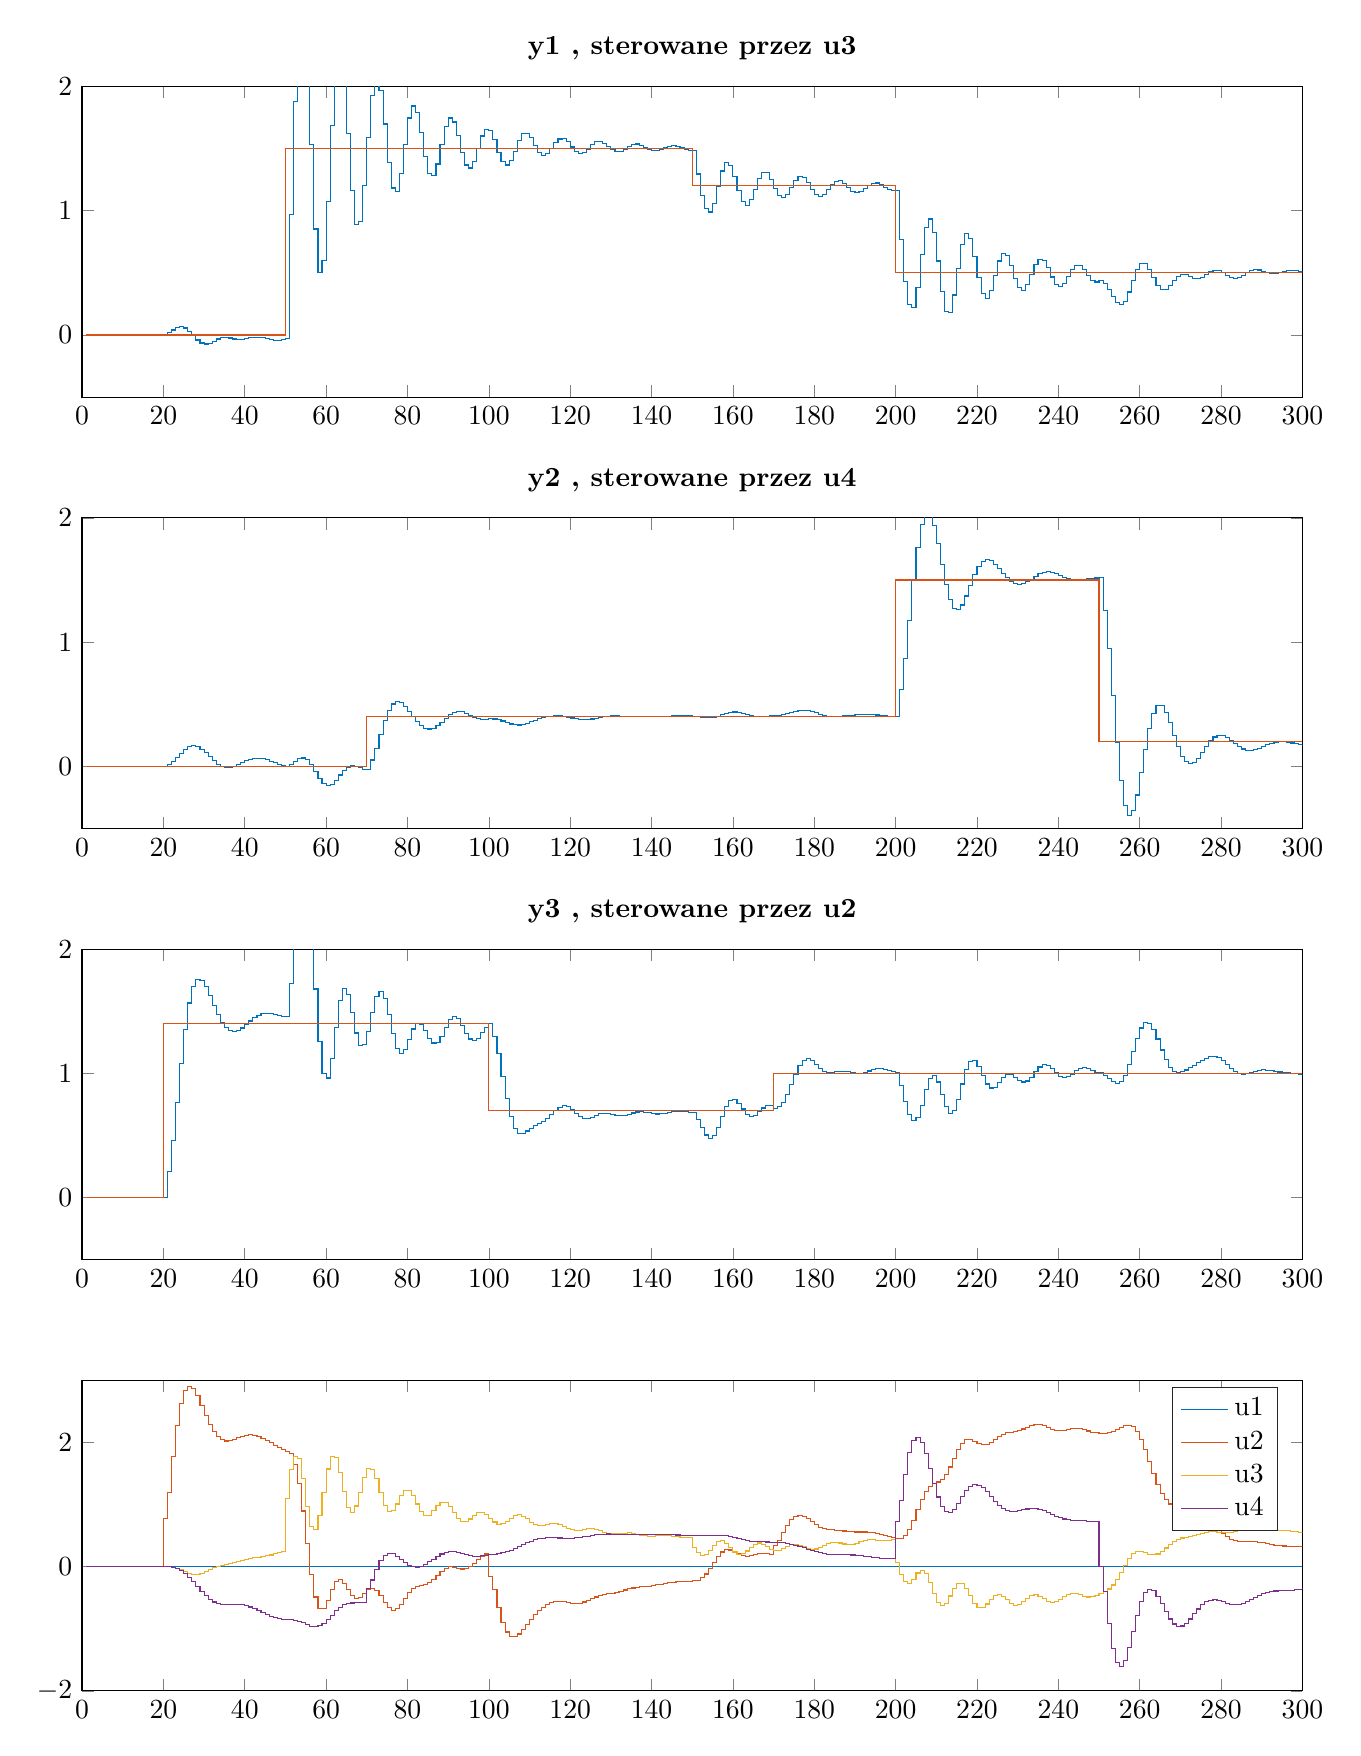
\begin{tikzpicture}

\begin{axis}[%
width=6.102in,
height=1.553in,
at={(1.024in,7.552in)},
scale only axis,
xmin=0,
xmax=300,
ymin=-0.5,
ymax=2,
axis background/.style={fill=white},
title style={font=\bfseries},
title={y1 , sterowane przez u3}
]
\addplot[const plot, color=mycolor1, forget plot] table[row sep=crcr] {%
1	0\\
2	0\\
3	0\\
4	0\\
5	0\\
6	0\\
7	0\\
8	0\\
9	0\\
10	0\\
11	0\\
12	0\\
13	0\\
14	0\\
15	0\\
16	0\\
17	0\\
18	0\\
19	0\\
20	0\\
21	0.0170323397035018\\
22	0.0395875063131282\\
23	0.0581256517899531\\
24	0.0657499527831088\\
25	0.056378977777873\\
26	0.030045762375443\\
27	-0.00593043850045157\\
28	-0.0407628430344126\\
29	-0.064761645512417\\
30	-0.0727811664016807\\
31	-0.0657539662259159\\
32	-0.0497205939743504\\
33	-0.0328378549382097\\
34	-0.0218533866835342\\
35	-0.0196182463784112\\
36	-0.0245626501375169\\
37	-0.0321270692777146\\
38	-0.0373069097326189\\
39	-0.0370682190676699\\
40	-0.0315740176665354\\
41	-0.0237957090746327\\
42	-0.0178458736521022\\
43	-0.0169091842394778\\
44	-0.0217497251855633\\
45	-0.0304301670871107\\
46	-0.0392819031734435\\
47	-0.0446017981334569\\
48	-0.0442675908210063\\
49	-0.0385620601608832\\
50	-0.0299003070925314\\
51	0.969188191011884\\
52	1.87912770062782\\
53	2.45478584680601\\
54	2.59982436316915\\
55	2.23358970550798\\
56	1.53235624181433\\
57	0.852575023373634\\
58	0.500848233655914\\
59	0.602263117359667\\
60	1.07597395539783\\
61	1.68702461449564\\
62	2.15887141454365\\
63	2.29910093592896\\
64	2.07751619956168\\
65	1.62490145099714\\
66	1.16124909323648\\
67	0.891449571917078\\
68	0.916774025261577\\
69	1.19963031248924\\
70	1.59249308550293\\
71	1.92995282770055\\
72	2.06871348144596\\
73	1.96834222008904\\
74	1.69780307608084\\
75	1.39069416478075\\
76	1.18291789688626\\
77	1.15433352347691\\
78	1.2985945832079\\
79	1.53392179891268\\
80	1.74636101803217\\
81	1.84304054900789\\
82	1.79117446343166\\
83	1.62706837398126\\
84	1.43382099327129\\
85	1.30031461230189\\
86	1.28126093460894\\
87	1.3758547403847\\
88	1.53282930237948\\
89	1.67738591988174\\
90	1.74622305076152\\
91	1.71451648987156\\
92	1.6036489076365\\
93	1.46793769783293\\
94	1.36800932328424\\
95	1.34368296378396\\
96	1.39832652823684\\
97	1.50056346073074\\
98	1.60106894012372\\
99	1.65575944258492\\
100	1.64463145930101\\
101	1.56984413363007\\
102	1.47104930911143\\
103	1.39314487135746\\
104	1.36772741860152\\
105	1.40269182126892\\
106	1.47952971026078\\
107	1.56297928543591\\
108	1.61804195371215\\
109	1.62516024607485\\
110	1.58713908968332\\
111	1.52579776219038\\
112	1.47068460349287\\
113	1.44543746103545\\
114	1.45799988869085\\
115	1.49865249427844\\
116	1.54600652543586\\
117	1.57759517485101\\
118	1.57998115028019\\
119	1.55396326857127\\
120	1.51301519643663\\
121	1.47623918618794\\
122	1.45942506687775\\
123	1.46832738559263\\
124	1.49693830774728\\
125	1.53109129346792\\
126	1.55535284190263\\
127	1.55988798565043\\
128	1.54428309119339\\
129	1.51690892290429\\
130	1.49049053591391\\
131	1.47615943584538\\
132	1.47873135137518\\
133	1.49517390047866\\
134	1.51665420063806\\
135	1.5329490747689\\
136	1.53706972136581\\
137	1.52804844891216\\
138	1.51082497198654\\
139	1.49353976435568\\
140	1.48365593536055\\
141	1.48472143232755\\
142	1.49514193052256\\
143	1.509328908097\\
144	1.52050937608889\\
145	1.52381436294332\\
146	1.51826133899867\\
147	1.50685367112068\\
148	1.49491695216931\\
149	1.48755768190046\\
150	1.48743879916193\\
151	1.29565313876841\\
152	1.12402851735685\\
153	1.01684530574357\\
154	0.990098193896167\\
155	1.05941978429037\\
156	1.1918040584466\\
157	1.31972753903257\\
158	1.38536907489535\\
159	1.36543421283996\\
160	1.27544441236866\\
161	1.15987246806848\\
162	1.07091519039253\\
163	1.04477370027654\\
164	1.08696724257292\\
165	1.17265240118411\\
166	1.26023524531436\\
167	1.31107519119854\\
168	1.30616147181905\\
169	1.25270713816548\\
170	1.1786308247805\\
171	1.12207163048294\\
172	1.1058545071592\\
173	1.13370655127117\\
174	1.18958617311634\\
175	1.24550414695375\\
176	1.27548976246334\\
177	1.2672351115607\\
178	1.22634151406981\\
179	1.17240152186864\\
180	1.12931023122371\\
181	1.11444197920881\\
182	1.13157397556213\\
183	1.17037949962068\\
184	1.21214151882104\\
185	1.23863525020527\\
186	1.24001187513303\\
187	1.21831714953225\\
188	1.18548814780766\\
189	1.15719849514084\\
190	1.14562503478683\\
191	1.15440988827738\\
192	1.17783590855855\\
193	1.20420134856803\\
194	1.22153312864121\\
195	1.22291331946434\\
196	1.20910451410849\\
197	1.18755349294799\\
198	1.16852914826794\\
199	1.16034718906114\\
200	1.16586605202865\\
201	0.766943570618794\\
202	0.433873851089612\\
203	0.246719216591434\\
204	0.224421706482628\\
205	0.384620505939519\\
206	0.645508761278916\\
207	0.864542764426292\\
208	0.933731763226269\\
209	0.826017233926177\\
210	0.595133823052753\\
211	0.346528762994656\\
212	0.188339580660371\\
213	0.182822692283507\\
214	0.321702107849333\\
215	0.535025399248663\\
216	0.726341484484008\\
217	0.816497022754781\\
218	0.776315080826176\\
219	0.634816772775001\\
220	0.461449708760414\\
221	0.332349006326017\\
222	0.296780393725915\\
223	0.358395821700555\\
224	0.478141680468486\\
225	0.595563957047881\\
226	0.657481684643927\\
227	0.640761328241194\\
228	0.559715763230446\\
229	0.456270120308051\\
230	0.378792555420591\\
231	0.359956821230466\\
232	0.40350948116613\\
233	0.485013541798045\\
234	0.565026198422646\\
235	0.607814199997435\\
236	0.596864344971441\\
237	0.540615195942057\\
238	0.466713517449296\\
239	0.40830088169119\\
240	0.38904342813957\\
241	0.413592388965911\\
242	0.467197248305548\\
243	0.523848301127809\\
244	0.558632572708578\\
245	0.5585137514207\\
246	0.526946827618786\\
247	0.480849797502025\\
248	0.441942319642302\\
249	0.426758188732053\\
250	0.439839576248428\\
251	0.41650661412262\\
252	0.369352160656983\\
253	0.312166222064041\\
254	0.260892864519967\\
255	0.241814476821195\\
256	0.271804414411372\\
257	0.345965470323668\\
258	0.44115614013243\\
259	0.52616715047772\\
260	0.57390261666483\\
261	0.571990623850947\\
262	0.527086014724493\\
263	0.460943161953742\\
264	0.400584924642834\\
265	0.367253938823978\\
266	0.368821398275303\\
267	0.398462869653902\\
268	0.439523439390325\\
269	0.473857839467652\\
270	0.48970975264506\\
271	0.485804034654264\\
272	0.470317968347502\\
273	0.455771237650923\\
274	0.452558658580355\\
275	0.464171715227779\\
276	0.486100296619446\\
277	0.508568293063716\\
278	0.521520684479409\\
279	0.519405083123315\\
280	0.503588453969321\\
281	0.481485171053281\\
282	0.463016763470731\\
283	0.45616571829533\\
284	0.463653552908394\\
285	0.482121603012315\\
286	0.503985920542999\\
287	0.520953537762866\\
288	0.527545075169664\\
289	0.523104567029524\\
290	0.51156552156521\\
291	0.49928112616434\\
292	0.49203942776736\\
293	0.492635286114283\\
294	0.499999930485316\\
295	0.510114177216306\\
296	0.518128730539183\\
297	0.520639179456895\\
298	0.517093788753301\\
299	0.509789867263031\\
300	0.502588862865703\\
};
\addplot[const plot, color=mycolor2, forget plot] table[row sep=crcr] {%
1	0\\
2	0\\
3	0\\
4	0\\
5	0\\
6	0\\
7	0\\
8	0\\
9	0\\
10	0\\
11	0\\
12	0\\
13	0\\
14	0\\
15	0\\
16	0\\
17	0\\
18	0\\
19	0\\
20	0\\
21	0\\
22	0\\
23	0\\
24	0\\
25	0\\
26	0\\
27	0\\
28	0\\
29	0\\
30	0\\
31	0\\
32	0\\
33	0\\
34	0\\
35	0\\
36	0\\
37	0\\
38	0\\
39	0\\
40	0\\
41	0\\
42	0\\
43	0\\
44	0\\
45	0\\
46	0\\
47	0\\
48	0\\
49	0\\
50	1.5\\
51	1.5\\
52	1.5\\
53	1.5\\
54	1.5\\
55	1.5\\
56	1.5\\
57	1.5\\
58	1.5\\
59	1.5\\
60	1.5\\
61	1.5\\
62	1.5\\
63	1.5\\
64	1.5\\
65	1.5\\
66	1.5\\
67	1.5\\
68	1.5\\
69	1.5\\
70	1.5\\
71	1.5\\
72	1.5\\
73	1.5\\
74	1.5\\
75	1.5\\
76	1.5\\
77	1.5\\
78	1.5\\
79	1.5\\
80	1.5\\
81	1.5\\
82	1.5\\
83	1.5\\
84	1.5\\
85	1.5\\
86	1.5\\
87	1.5\\
88	1.5\\
89	1.5\\
90	1.5\\
91	1.5\\
92	1.5\\
93	1.5\\
94	1.5\\
95	1.5\\
96	1.5\\
97	1.5\\
98	1.5\\
99	1.5\\
100	1.5\\
101	1.5\\
102	1.5\\
103	1.5\\
104	1.5\\
105	1.5\\
106	1.5\\
107	1.5\\
108	1.5\\
109	1.5\\
110	1.5\\
111	1.5\\
112	1.5\\
113	1.5\\
114	1.5\\
115	1.5\\
116	1.5\\
117	1.5\\
118	1.5\\
119	1.5\\
120	1.5\\
121	1.5\\
122	1.5\\
123	1.5\\
124	1.5\\
125	1.5\\
126	1.5\\
127	1.5\\
128	1.5\\
129	1.5\\
130	1.5\\
131	1.5\\
132	1.5\\
133	1.5\\
134	1.5\\
135	1.5\\
136	1.5\\
137	1.5\\
138	1.5\\
139	1.5\\
140	1.5\\
141	1.5\\
142	1.5\\
143	1.5\\
144	1.5\\
145	1.5\\
146	1.5\\
147	1.5\\
148	1.5\\
149	1.5\\
150	1.2\\
151	1.2\\
152	1.2\\
153	1.2\\
154	1.2\\
155	1.2\\
156	1.2\\
157	1.2\\
158	1.2\\
159	1.2\\
160	1.2\\
161	1.2\\
162	1.2\\
163	1.2\\
164	1.2\\
165	1.2\\
166	1.2\\
167	1.2\\
168	1.2\\
169	1.2\\
170	1.2\\
171	1.2\\
172	1.2\\
173	1.2\\
174	1.2\\
175	1.2\\
176	1.2\\
177	1.2\\
178	1.2\\
179	1.2\\
180	1.2\\
181	1.2\\
182	1.2\\
183	1.2\\
184	1.2\\
185	1.2\\
186	1.2\\
187	1.2\\
188	1.2\\
189	1.2\\
190	1.2\\
191	1.2\\
192	1.2\\
193	1.2\\
194	1.2\\
195	1.2\\
196	1.2\\
197	1.2\\
198	1.2\\
199	1.2\\
200	0.5\\
201	0.5\\
202	0.5\\
203	0.5\\
204	0.5\\
205	0.5\\
206	0.5\\
207	0.5\\
208	0.5\\
209	0.5\\
210	0.5\\
211	0.5\\
212	0.5\\
213	0.5\\
214	0.5\\
215	0.5\\
216	0.5\\
217	0.5\\
218	0.5\\
219	0.5\\
220	0.5\\
221	0.5\\
222	0.5\\
223	0.5\\
224	0.5\\
225	0.5\\
226	0.5\\
227	0.5\\
228	0.5\\
229	0.5\\
230	0.5\\
231	0.5\\
232	0.5\\
233	0.5\\
234	0.5\\
235	0.5\\
236	0.5\\
237	0.5\\
238	0.5\\
239	0.5\\
240	0.5\\
241	0.5\\
242	0.5\\
243	0.5\\
244	0.5\\
245	0.5\\
246	0.5\\
247	0.5\\
248	0.5\\
249	0.5\\
250	0.5\\
251	0.5\\
252	0.5\\
253	0.5\\
254	0.5\\
255	0.5\\
256	0.5\\
257	0.5\\
258	0.5\\
259	0.5\\
260	0.5\\
261	0.5\\
262	0.5\\
263	0.5\\
264	0.5\\
265	0.5\\
266	0.5\\
267	0.5\\
268	0.5\\
269	0.5\\
270	0.5\\
271	0.5\\
272	0.5\\
273	0.5\\
274	0.5\\
275	0.5\\
276	0.5\\
277	0.5\\
278	0.5\\
279	0.5\\
280	0.5\\
281	0.5\\
282	0.5\\
283	0.5\\
284	0.5\\
285	0.5\\
286	0.5\\
287	0.5\\
288	0.5\\
289	0.5\\
290	0.5\\
291	0.5\\
292	0.5\\
293	0.5\\
294	0.5\\
295	0.5\\
296	0.5\\
297	0.5\\
298	0.5\\
299	0.5\\
300	0.5\\
};
\end{axis}

\begin{axis}[%
width=6.102in,
height=1.553in,
at={(1.024in,5.395in)},
scale only axis,
xmin=0,
xmax=300,
ymin=-0.5,
ymax=2,
axis background/.style={fill=white},
title style={font=\bfseries},
title={y2 , sterowane przez u4}
]
\addplot[const plot, color=mycolor1, forget plot] table[row sep=crcr] {%
1	0\\
2	0\\
3	0\\
4	0\\
5	0\\
6	0\\
7	0\\
8	0\\
9	0\\
10	0\\
11	0\\
12	0\\
13	0\\
14	0\\
15	0\\
16	0\\
17	0\\
18	0\\
19	0\\
20	0\\
21	0.0157120590129818\\
22	0.0393531143747916\\
23	0.0705244041418738\\
24	0.104860355922353\\
25	0.135563941631857\\
26	0.15686597735678\\
27	0.164985780569781\\
28	0.158668233345662\\
29	0.139330140987265\\
30	0.110589720331562\\
31	0.0773757684872827\\
32	0.0448912531125219\\
33	0.0176669972552193\\
34	-0.00112349500994854\\
35	-0.0100054830744118\\
36	-0.00920528292071796\\
37	-0.000380806385424322\\
38	0.0138223078669189\\
39	0.030290357009038\\
40	0.045954042799196\\
41	0.0582310773530513\\
42	0.0653540113075448\\
43	0.0665527090498628\\
44	0.0620753489971609\\
45	0.0530503641000593\\
46	0.0412150940518492\\
47	0.02856111378026\\
48	0.0169639102775331\\
49	0.00786855031281506\\
50	0.00208971097416652\\
51	0.0154581337983441\\
52	0.0388698279731004\\
53	0.0598025631410659\\
54	0.067774979834696\\
55	0.0533249751008136\\
56	0.0143325190962992\\
57	-0.0410449421001609\\
58	-0.0978543349081722\\
59	-0.140215585151262\\
60	-0.156982883142891\\
61	-0.14554106079645\\
62	-0.112250349064842\\
63	-0.0694282785691685\\
64	-0.0303829775874987\\
65	-0.00468558236118374\\
66	0.00449462636378639\\
67	0.000208155889922006\\
68	-0.0108363973660002\\
69	-0.0218121765937055\\
70	-0.0286558085220972\\
71	0.0510814246043967\\
72	0.144938741972324\\
73	0.257254767217376\\
74	0.365955727320507\\
75	0.450402529486227\\
76	0.501817721637405\\
77	0.520098462237279\\
78	0.510778063264523\\
79	0.482212002274428\\
80	0.443048628254775\\
81	0.400757941380243\\
82	0.361270818758059\\
83	0.329225598999858\\
84	0.308218244251773\\
85	0.30067337317558\\
86	0.307334665279671\\
87	0.326707558555036\\
88	0.354905857072378\\
89	0.386208611270463\\
90	0.414308501360586\\
91	0.43389386055264\\
92	0.442018300666354\\
93	0.438762369510628\\
94	0.426955839542813\\
95	0.411087337457199\\
96	0.395824441313046\\
97	0.384681324048231\\
98	0.379266937257507\\
99	0.37928358118714\\
100	0.383144507127186\\
101	0.381010194106507\\
102	0.375167138612624\\
103	0.364972311228357\\
104	0.352461236262936\\
105	0.34120658343241\\
106	0.334164747959463\\
107	0.332957163753094\\
108	0.337657485411983\\
109	0.347013940792895\\
110	0.359045443346314\\
111	0.371712845430234\\
112	0.383400210409728\\
113	0.393090427514566\\
114	0.40027513338102\\
115	0.404743776175685\\
116	0.406414427940124\\
117	0.405304727867794\\
118	0.401637390893806\\
119	0.395986643119924\\
120	0.389341982434966\\
121	0.383004480554788\\
122	0.378315417162448\\
123	0.376304117706454\\
124	0.377389440976352\\
125	0.381255825181655\\
126	0.386957483864747\\
127	0.393214428350655\\
128	0.39879113291248\\
129	0.402822931671186\\
130	0.404984640171862\\
131	0.405464443598088\\
132	0.404782514683755\\
133	0.403546190848952\\
134	0.402242966125009\\
135	0.401140067872866\\
136	0.40030359300185\\
137	0.399697531404997\\
138	0.399295625642698\\
139	0.399145556568827\\
140	0.399358218104374\\
141	0.400036621383586\\
142	0.401189158271795\\
143	0.402677724072924\\
144	0.404232016971682\\
145	0.405528077542286\\
146	0.406298208716456\\
147	0.406424916489954\\
148	0.405979078936712\\
149	0.405187521695213\\
150	0.404345452394034\\
151	0.40057082110011\\
152	0.395730491801861\\
153	0.392146776405328\\
154	0.391582626608876\\
155	0.395559174393281\\
156	0.404198891031009\\
157	0.415705368332466\\
158	0.427069728505569\\
159	0.435204970772359\\
160	0.438014236377853\\
161	0.435091318857415\\
162	0.427778008775776\\
163	0.418562143604229\\
164	0.410109405512193\\
165	0.40434751949551\\
166	0.401949599562766\\
167	0.402364791778935\\
168	0.404306509382324\\
169	0.406431222493918\\
170	0.407896203298355\\
171	0.411945948442267\\
172	0.417351775533588\\
173	0.424624591089067\\
174	0.433160051887995\\
175	0.441335778342076\\
176	0.447309141905722\\
177	0.449520359575273\\
178	0.447187428846428\\
179	0.440612850519472\\
180	0.431125497125564\\
181	0.420684882375759\\
182	0.411304502769579\\
183	0.404504229242476\\
184	0.400974894681644\\
185	0.400542872123678\\
186	0.402402285345325\\
187	0.405488770348316\\
188	0.408836470138837\\
189	0.411794978432615\\
190	0.414062179017953\\
191	0.41557329825381\\
192	0.416339425461359\\
193	0.416331667938448\\
194	0.415465518636381\\
195	0.413678549498906\\
196	0.411044003784808\\
197	0.407845844239636\\
198	0.404562366269921\\
199	0.401752451524423\\
200	0.399887107244322\\
201	0.618015283233366\\
202	0.868305013977901\\
203	1.17728313896809\\
204	1.49344253229058\\
205	1.76116275730665\\
206	1.94751105979054\\
207	2.036635775703\\
208	2.02867617306232\\
209	1.93879667609298\\
210	1.7934654078859\\
211	1.6251518555026\\
212	1.46634411142566\\
213	1.34377803344178\\
214	1.27404566908188\\
215	1.26155410952659\\
216	1.29921410968004\\
217	1.37151931378239\\
218	1.45905834616155\\
219	1.54318697561909\\
220	1.60968286803386\\
221	1.65065505296598\\
222	1.66459574181854\\
223	1.65501240928064\\
224	1.62838306920884\\
225	1.59217232779848\\
226	1.55339215039083\\
227	1.51783744120453\\
228	1.48983427092614\\
229	1.47221413865519\\
230	1.46628502494373\\
231	1.47173870127882\\
232	1.48660267361829\\
233	1.50741911251672\\
234	1.52977592924304\\
235	1.5491608401085\\
236	1.56193992007673\\
237	1.56616530697593\\
238	1.56194341315185\\
239	1.55123754504494\\
240	1.53717683269532\\
241	1.52311322487363\\
242	1.51174127081626\\
243	1.50454674453709\\
244	1.50170709929366\\
245	1.50239334020866\\
246	1.50529023912937\\
247	1.50910750766571\\
248	1.51290495878498\\
249	1.51616636686632\\
250	1.51867472231549\\
251	1.25305109758477\\
252	0.945787425337792\\
253	0.571325972422098\\
254	0.19499934240734\\
255	-0.113288340246163\\
256	-0.313864843220647\\
257	-0.392187756358915\\
258	-0.355825378034298\\
259	-0.230453924987634\\
260	-0.0527298018676131\\
261	0.137820776446464\\
262	0.306095553400032\\
263	0.426757958984683\\
264	0.486977128303179\\
265	0.48648798905513\\
266	0.435422454160685\\
267	0.350712287768208\\
268	0.2519853058483\\
269	0.157784702981899\\
270	0.0827013521040482\\
271	0.0357096447936327\\
272	0.0197206406925033\\
273	0.0321649334168343\\
274	0.0663082271856067\\
275	0.112971768420312\\
276	0.162349701371976\\
277	0.20566013730182\\
278	0.236421964746367\\
279	0.251213294218909\\
280	0.249843708077704\\
281	0.234961496864613\\
282	0.211209588502061\\
283	0.184121472237164\\
284	0.158989924260741\\
285	0.139932229815246\\
286	0.129315480174519\\
287	0.127610084658553\\
288	0.133635911622944\\
289	0.145082437763185\\
290	0.15914275717804\\
291	0.173107262876211\\
292	0.184806689007198\\
293	0.192855962639625\\
294	0.19670790251044\\
295	0.196563238352314\\
296	0.193195422379178\\
297	0.187740411151181\\
298	0.181484231686085\\
299	0.175665947494749\\
300	0.171306925323758\\
};
\addplot[const plot, color=mycolor2, forget plot] table[row sep=crcr] {%
1	0\\
2	0\\
3	0\\
4	0\\
5	0\\
6	0\\
7	0\\
8	0\\
9	0\\
10	0\\
11	0\\
12	0\\
13	0\\
14	0\\
15	0\\
16	0\\
17	0\\
18	0\\
19	0\\
20	0\\
21	0\\
22	0\\
23	0\\
24	0\\
25	0\\
26	0\\
27	0\\
28	0\\
29	0\\
30	0\\
31	0\\
32	0\\
33	0\\
34	0\\
35	0\\
36	0\\
37	0\\
38	0\\
39	0\\
40	0\\
41	0\\
42	0\\
43	0\\
44	0\\
45	0\\
46	0\\
47	0\\
48	0\\
49	0\\
50	0\\
51	0\\
52	0\\
53	0\\
54	0\\
55	0\\
56	0\\
57	0\\
58	0\\
59	0\\
60	0\\
61	0\\
62	0\\
63	0\\
64	0\\
65	0\\
66	0\\
67	0\\
68	0\\
69	0\\
70	0.4\\
71	0.4\\
72	0.4\\
73	0.4\\
74	0.4\\
75	0.4\\
76	0.4\\
77	0.4\\
78	0.4\\
79	0.4\\
80	0.4\\
81	0.4\\
82	0.4\\
83	0.4\\
84	0.4\\
85	0.4\\
86	0.4\\
87	0.4\\
88	0.4\\
89	0.4\\
90	0.4\\
91	0.4\\
92	0.4\\
93	0.4\\
94	0.4\\
95	0.4\\
96	0.4\\
97	0.4\\
98	0.4\\
99	0.4\\
100	0.4\\
101	0.4\\
102	0.4\\
103	0.4\\
104	0.4\\
105	0.4\\
106	0.4\\
107	0.4\\
108	0.4\\
109	0.4\\
110	0.4\\
111	0.4\\
112	0.4\\
113	0.4\\
114	0.4\\
115	0.4\\
116	0.4\\
117	0.4\\
118	0.4\\
119	0.4\\
120	0.4\\
121	0.4\\
122	0.4\\
123	0.4\\
124	0.4\\
125	0.4\\
126	0.4\\
127	0.4\\
128	0.4\\
129	0.4\\
130	0.4\\
131	0.4\\
132	0.4\\
133	0.4\\
134	0.4\\
135	0.4\\
136	0.4\\
137	0.4\\
138	0.4\\
139	0.4\\
140	0.4\\
141	0.4\\
142	0.4\\
143	0.4\\
144	0.4\\
145	0.4\\
146	0.4\\
147	0.4\\
148	0.4\\
149	0.4\\
150	0.4\\
151	0.4\\
152	0.4\\
153	0.4\\
154	0.4\\
155	0.4\\
156	0.4\\
157	0.4\\
158	0.4\\
159	0.4\\
160	0.4\\
161	0.4\\
162	0.4\\
163	0.4\\
164	0.4\\
165	0.4\\
166	0.4\\
167	0.4\\
168	0.4\\
169	0.4\\
170	0.4\\
171	0.4\\
172	0.4\\
173	0.4\\
174	0.4\\
175	0.4\\
176	0.4\\
177	0.4\\
178	0.4\\
179	0.4\\
180	0.4\\
181	0.4\\
182	0.4\\
183	0.4\\
184	0.4\\
185	0.4\\
186	0.4\\
187	0.4\\
188	0.4\\
189	0.4\\
190	0.4\\
191	0.4\\
192	0.4\\
193	0.4\\
194	0.4\\
195	0.4\\
196	0.4\\
197	0.4\\
198	0.4\\
199	0.4\\
200	1.5\\
201	1.5\\
202	1.5\\
203	1.5\\
204	1.5\\
205	1.5\\
206	1.5\\
207	1.5\\
208	1.5\\
209	1.5\\
210	1.5\\
211	1.5\\
212	1.5\\
213	1.5\\
214	1.5\\
215	1.5\\
216	1.5\\
217	1.5\\
218	1.5\\
219	1.5\\
220	1.5\\
221	1.5\\
222	1.5\\
223	1.5\\
224	1.5\\
225	1.5\\
226	1.5\\
227	1.5\\
228	1.5\\
229	1.5\\
230	1.5\\
231	1.5\\
232	1.5\\
233	1.5\\
234	1.5\\
235	1.5\\
236	1.5\\
237	1.5\\
238	1.5\\
239	1.5\\
240	1.5\\
241	1.5\\
242	1.5\\
243	1.5\\
244	1.5\\
245	1.5\\
246	1.5\\
247	1.5\\
248	1.5\\
249	1.5\\
250	0.2\\
251	0.2\\
252	0.2\\
253	0.2\\
254	0.2\\
255	0.2\\
256	0.2\\
257	0.2\\
258	0.2\\
259	0.2\\
260	0.2\\
261	0.2\\
262	0.2\\
263	0.2\\
264	0.2\\
265	0.2\\
266	0.2\\
267	0.2\\
268	0.2\\
269	0.2\\
270	0.2\\
271	0.2\\
272	0.2\\
273	0.2\\
274	0.2\\
275	0.2\\
276	0.2\\
277	0.2\\
278	0.2\\
279	0.2\\
280	0.2\\
281	0.2\\
282	0.2\\
283	0.2\\
284	0.2\\
285	0.2\\
286	0.2\\
287	0.2\\
288	0.2\\
289	0.2\\
290	0.2\\
291	0.2\\
292	0.2\\
293	0.2\\
294	0.2\\
295	0.2\\
296	0.2\\
297	0.2\\
298	0.2\\
299	0.2\\
300	0.2\\
};
\end{axis}

\begin{axis}[%
width=6.102in,
height=1.553in,
at={(1.024in,3.239in)},
scale only axis,
xmin=0,
xmax=300,
ymin=-0.5,
ymax=2,
axis background/.style={fill=white},
title style={font=\bfseries},
title={y3 , sterowane przez u2}
]
\addplot[const plot, color=mycolor1, forget plot] table[row sep=crcr] {%
1	0\\
2	0\\
3	0\\
4	0\\
5	0\\
6	0\\
7	0\\
8	0\\
9	0\\
10	0\\
11	0\\
12	0\\
13	0\\
14	0\\
15	0\\
16	0\\
17	0\\
18	0\\
19	0\\
20	0\\
21	0.212079974414891\\
22	0.456392967253078\\
23	0.761809299385984\\
24	1.07821341141774\\
25	1.35592813430686\\
26	1.56645745046573\\
27	1.69819554032618\\
28	1.75392288571174\\
29	1.74718860758948\\
30	1.69723789358563\\
31	1.62406642209801\\
32	1.54476579265501\\
33	1.47168458615675\\
34	1.41227436788954\\
35	1.37001771258959\\
36	1.34568948368177\\
37	1.33836221443669\\
38	1.34591309426937\\
39	1.3651479772461\\
40	1.39186561676039\\
41	1.42117216194068\\
42	1.44816305576894\\
43	1.46883596394813\\
44	1.48091865706503\\
45	1.4842773801535\\
46	1.48071881358695\\
47	1.47323846899794\\
48	1.46498768623431\\
49	1.45833279742328\\
50	1.45432391162295\\
51	1.72644320366658\\
52	2.08863555659259\\
53	2.39695738336616\\
54	2.55030998771614\\
55	2.46042047948711\\
56	2.13250803631493\\
57	1.67871651158055\\
58	1.25620634704575\\
59	0.997723782181178\\
60	0.962826064185038\\
61	1.12041514113026\\
62	1.36937097257888\\
63	1.58754202506226\\
64	1.68498730460178\\
65	1.63772512384837\\
66	1.48956615527918\\
67	1.32450696572799\\
68	1.22455721591285\\
69	1.23287660879635\\
70	1.33794080076469\\
71	1.49216488948102\\
72	1.61912160417822\\
73	1.66220365647628\\
74	1.60419029754557\\
75	1.47091818548795\\
76	1.31734432069611\\
77	1.2017022391924\\
78	1.16041211983824\\
79	1.19495933203323\\
80	1.27529634743159\\
81	1.35656374889112\\
82	1.40049029474186\\
83	1.39162346681634\\
84	1.34171699885025\\
85	1.28145423972305\\
86	1.24438558052119\\
87	1.25097818876651\\
88	1.29992614309715\\
89	1.37001913535995\\
90	1.43088922493258\\
91	1.45714496701899\\
92	1.43934463708038\\
93	1.38718741239036\\
94	1.32410848934026\\
95	1.27631297712932\\
96	1.26147554701911\\
97	1.28204507131793\\
98	1.32566447064575\\
99	1.37189640623337\\
100	1.4017688419644\\
101	1.29969844541575\\
102	1.15856446235162\\
103	0.976695649938973\\
104	0.795003044377482\\
105	0.64986008651304\\
106	0.557966531064042\\
107	0.518232468834581\\
108	0.516974369092982\\
109	0.535743032563994\\
110	0.559094368580759\\
111	0.579250602958298\\
112	0.596353290682866\\
113	0.615056260621638\\
114	0.639665908676516\\
115	0.670361261602913\\
116	0.702196428231922\\
117	0.727097407964658\\
118	0.737638205126005\\
119	0.730643967608609\\
120	0.708887556888797\\
121	0.680137733606403\\
122	0.65407071167669\\
123	0.638489159634744\\
124	0.636513440602163\\
125	0.645876978583937\\
126	0.660466228047155\\
127	0.673269073967851\\
128	0.679361110520396\\
129	0.677664416692572\\
130	0.670858051544286\\
131	0.663675529291949\\
132	0.660499826480989\\
133	0.663382374495793\\
134	0.671316225522667\\
135	0.680961523272369\\
136	0.688361407477272\\
137	0.690791010855642\\
138	0.687901247532179\\
139	0.681706863757353\\
140	0.675520715791208\\
141	0.67239502720306\\
142	0.673801198943387\\
143	0.679112397451732\\
144	0.686050919323\\
145	0.691823036269185\\
146	0.694384575092817\\
147	0.693270240375869\\
148	0.689659917392431\\
149	0.685718503306465\\
150	0.68356169389139\\
151	0.629586974346828\\
152	0.560546420846659\\
153	0.503581017521776\\
154	0.476905867759241\\
155	0.496712765853961\\
156	0.561608756165932\\
157	0.649958817766594\\
158	0.731794640925981\\
159	0.781981684612413\\
160	0.789348216142137\\
161	0.759912520393516\\
162	0.712933584920225\\
163	0.671614133143733\\
164	0.653025494686439\\
165	0.661742447458449\\
166	0.689518416231247\\
167	0.720516965823494\\
168	0.739281912591203\\
169	0.737691500923244\\
170	0.717934180449446\\
171	0.736020088368396\\
172	0.76682828294321\\
173	0.826489671516452\\
174	0.906494652912657\\
175	0.990265118087433\\
176	1.06082532931827\\
177	1.10504487141988\\
178	1.11775556101232\\
179	1.10310783329342\\
180	1.07236394899684\\
181	1.03923202788303\\
182	1.01478442007427\\
183	1.00401760812874\\
184	1.00525257256633\\
185	1.01227826081238\\
186	1.01800436946143\\
187	1.01788675218478\\
188	1.01168054605472\\
189	1.00296323297751\\
190	0.996909466800063\\
191	0.997522731477846\\
192	1.00564901543796\\
193	1.01861890852608\\
194	1.03155391695514\\
195	1.03961933763527\\
196	1.04013848066562\\
197	1.03363037045062\\
198	1.0233853817442\\
199	1.01387130269014\\
200	1.00875544822128\\
201	0.904911537545906\\
202	0.773301697095114\\
203	0.66750884330555\\
204	0.616921752064453\\
205	0.645655480308301\\
206	0.744181806512282\\
207	0.86689661776019\\
208	0.95884027814585\\
209	0.98194743191362\\
210	0.930099249524377\\
211	0.830647885106871\\
212	0.731594319603118\\
213	0.67989716944779\\
214	0.701243320323865\\
215	0.79021047234751\\
216	0.914276789850656\\
217	1.02893066012527\\
218	1.0966353171578\\
219	1.1013073733005\\
220	1.0525764046905\\
221	0.978981130326449\\
222	0.914073943934893\\
223	0.882059316201977\\
224	0.889132780873604\\
225	0.923601445333155\\
226	0.963741117232518\\
227	0.989078615036155\\
228	0.989729982624936\\
229	0.969832084007538\\
230	0.944125971116858\\
231	0.929902703921573\\
232	0.938400166043461\\
233	0.969626409761845\\
234	1.01270848822826\\
235	1.0512126692407\\
236	1.07069658817528\\
237	1.06496584104493\\
238	1.03834865030923\\
239	1.00326483484509\\
240	0.974489749307047\\
241	0.962850506262796\\
242	0.971118553624367\\
243	0.993678075454577\\
244	1.01977609467213\\
245	1.0386249599309\\
246	1.04398216423855\\
247	1.03628032701132\\
248	1.02162836587213\\
249	1.00843509413712\\
250	1.00337556602757\\
251	0.981103732340472\\
252	0.955310070556513\\
253	0.931487263343468\\
254	0.919837629313489\\
255	0.934333382602274\\
256	0.984125668763896\\
257	1.06806943556437\\
258	1.17374733120748\\
259	1.28039340002267\\
260	1.36484297672747\\
261	1.40868081210211\\
262	1.40389796147353\\
263	1.35490721281996\\
264	1.27637637052547\\
265	1.18798495217973\\
266	1.10824094202363\\
267	1.04961965785586\\
268	1.01652174259114\\
269	1.00627250504717\\
270	1.01218440814079\\
271	1.02706984877401\\
272	1.04571445429802\\
273	1.06555067127428\\
274	1.08571473799769\\
275	1.10538669038879\\
276	1.12251204699027\\
277	1.13365713667387\\
278	1.13507782295671\\
279	1.1244291429982\\
280	1.10221520236812\\
281	1.07220424237455\\
282	1.040525081848\\
283	1.01376997299376\\
284	0.996871258480228\\
285	0.991605116450106\\
286	0.99628684289402\\
287	1.00670714386318\\
288	1.01785508277779\\
289	1.02569562461687\\
290	1.02831859734896\\
291	1.02610286264687\\
292	1.02098069173344\\
293	1.0152446125178\\
294	1.01046882842667\\
295	1.00698811568349\\
296	1.00407248509364\\
297	1.00060733168896\\
298	0.995883023117604\\
299	0.990093034352338\\
300	0.984317539034508\\
};
\addplot[const plot, color=mycolor2, forget plot] table[row sep=crcr] {%
1	0\\
2	0\\
3	0\\
4	0\\
5	0\\
6	0\\
7	0\\
8	0\\
9	0\\
10	0\\
11	0\\
12	0\\
13	0\\
14	0\\
15	0\\
16	0\\
17	0\\
18	0\\
19	0\\
20	1.4\\
21	1.4\\
22	1.4\\
23	1.4\\
24	1.4\\
25	1.4\\
26	1.4\\
27	1.4\\
28	1.4\\
29	1.4\\
30	1.4\\
31	1.4\\
32	1.4\\
33	1.4\\
34	1.4\\
35	1.4\\
36	1.4\\
37	1.4\\
38	1.4\\
39	1.4\\
40	1.4\\
41	1.4\\
42	1.4\\
43	1.4\\
44	1.4\\
45	1.4\\
46	1.4\\
47	1.4\\
48	1.4\\
49	1.4\\
50	1.4\\
51	1.4\\
52	1.4\\
53	1.4\\
54	1.4\\
55	1.4\\
56	1.4\\
57	1.4\\
58	1.4\\
59	1.4\\
60	1.4\\
61	1.4\\
62	1.4\\
63	1.4\\
64	1.4\\
65	1.4\\
66	1.4\\
67	1.4\\
68	1.4\\
69	1.4\\
70	1.4\\
71	1.4\\
72	1.4\\
73	1.4\\
74	1.4\\
75	1.4\\
76	1.4\\
77	1.4\\
78	1.4\\
79	1.4\\
80	1.4\\
81	1.4\\
82	1.4\\
83	1.4\\
84	1.4\\
85	1.4\\
86	1.4\\
87	1.4\\
88	1.4\\
89	1.4\\
90	1.4\\
91	1.4\\
92	1.4\\
93	1.4\\
94	1.4\\
95	1.4\\
96	1.4\\
97	1.4\\
98	1.4\\
99	1.4\\
100	0.7\\
101	0.7\\
102	0.7\\
103	0.7\\
104	0.7\\
105	0.7\\
106	0.7\\
107	0.7\\
108	0.7\\
109	0.7\\
110	0.7\\
111	0.7\\
112	0.7\\
113	0.7\\
114	0.7\\
115	0.7\\
116	0.7\\
117	0.7\\
118	0.7\\
119	0.7\\
120	0.7\\
121	0.7\\
122	0.7\\
123	0.7\\
124	0.7\\
125	0.7\\
126	0.7\\
127	0.7\\
128	0.7\\
129	0.7\\
130	0.7\\
131	0.7\\
132	0.7\\
133	0.7\\
134	0.7\\
135	0.7\\
136	0.7\\
137	0.7\\
138	0.7\\
139	0.7\\
140	0.7\\
141	0.7\\
142	0.7\\
143	0.7\\
144	0.7\\
145	0.7\\
146	0.7\\
147	0.7\\
148	0.7\\
149	0.7\\
150	0.7\\
151	0.7\\
152	0.7\\
153	0.7\\
154	0.7\\
155	0.7\\
156	0.7\\
157	0.7\\
158	0.7\\
159	0.7\\
160	0.7\\
161	0.7\\
162	0.7\\
163	0.7\\
164	0.7\\
165	0.7\\
166	0.7\\
167	0.7\\
168	0.7\\
169	0.7\\
170	1\\
171	1\\
172	1\\
173	1\\
174	1\\
175	1\\
176	1\\
177	1\\
178	1\\
179	1\\
180	1\\
181	1\\
182	1\\
183	1\\
184	1\\
185	1\\
186	1\\
187	1\\
188	1\\
189	1\\
190	1\\
191	1\\
192	1\\
193	1\\
194	1\\
195	1\\
196	1\\
197	1\\
198	1\\
199	1\\
200	1\\
201	1\\
202	1\\
203	1\\
204	1\\
205	1\\
206	1\\
207	1\\
208	1\\
209	1\\
210	1\\
211	1\\
212	1\\
213	1\\
214	1\\
215	1\\
216	1\\
217	1\\
218	1\\
219	1\\
220	1\\
221	1\\
222	1\\
223	1\\
224	1\\
225	1\\
226	1\\
227	1\\
228	1\\
229	1\\
230	1\\
231	1\\
232	1\\
233	1\\
234	1\\
235	1\\
236	1\\
237	1\\
238	1\\
239	1\\
240	1\\
241	1\\
242	1\\
243	1\\
244	1\\
245	1\\
246	1\\
247	1\\
248	1\\
249	1\\
250	1\\
251	1\\
252	1\\
253	1\\
254	1\\
255	1\\
256	1\\
257	1\\
258	1\\
259	1\\
260	1\\
261	1\\
262	1\\
263	1\\
264	1\\
265	1\\
266	1\\
267	1\\
268	1\\
269	1\\
270	1\\
271	1\\
272	1\\
273	1\\
274	1\\
275	1\\
276	1\\
277	1\\
278	1\\
279	1\\
280	1\\
281	1\\
282	1\\
283	1\\
284	1\\
285	1\\
286	1\\
287	1\\
288	1\\
289	1\\
290	1\\
291	1\\
292	1\\
293	1\\
294	1\\
295	1\\
296	1\\
297	1\\
298	1\\
299	1\\
300	1\\
};
\end{axis}

\begin{axis}[%
width=6.102in,
height=1.553in,
at={(1.024in,1.083in)},
scale only axis,
xmin=0,
xmax=300,
ymin=-2,
ymax=3,
axis background/.style={fill=white},
legend style={legend cell align=left, align=left, draw=white!15!black}
]
\addplot[const plot, color=mycolor1] table[row sep=crcr] {%
1	0\\
2	0\\
3	0\\
4	0\\
5	0\\
6	0\\
7	0\\
8	0\\
9	0\\
10	0\\
11	0\\
12	0\\
13	0\\
14	0\\
15	0\\
16	0\\
17	0\\
18	0\\
19	0\\
20	0\\
21	0\\
22	0\\
23	0\\
24	0\\
25	0\\
26	0\\
27	0\\
28	0\\
29	0\\
30	0\\
31	0\\
32	0\\
33	0\\
34	0\\
35	0\\
36	0\\
37	0\\
38	0\\
39	0\\
40	0\\
41	0\\
42	0\\
43	0\\
44	0\\
45	0\\
46	0\\
47	0\\
48	0\\
49	0\\
50	0\\
51	0\\
52	0\\
53	0\\
54	0\\
55	0\\
56	0\\
57	0\\
58	0\\
59	0\\
60	0\\
61	0\\
62	0\\
63	0\\
64	0\\
65	0\\
66	0\\
67	0\\
68	0\\
69	0\\
70	0\\
71	0\\
72	0\\
73	0\\
74	0\\
75	0\\
76	0\\
77	0\\
78	0\\
79	0\\
80	0\\
81	0\\
82	0\\
83	0\\
84	0\\
85	0\\
86	0\\
87	0\\
88	0\\
89	0\\
90	0\\
91	0\\
92	0\\
93	0\\
94	0\\
95	0\\
96	0\\
97	0\\
98	0\\
99	0\\
100	0\\
101	0\\
102	0\\
103	0\\
104	0\\
105	0\\
106	0\\
107	0\\
108	0\\
109	0\\
110	0\\
111	0\\
112	0\\
113	0\\
114	0\\
115	0\\
116	0\\
117	0\\
118	0\\
119	0\\
120	0\\
121	0\\
122	0\\
123	0\\
124	0\\
125	0\\
126	0\\
127	0\\
128	0\\
129	0\\
130	0\\
131	0\\
132	0\\
133	0\\
134	0\\
135	0\\
136	0\\
137	0\\
138	0\\
139	0\\
140	0\\
141	0\\
142	0\\
143	0\\
144	0\\
145	0\\
146	0\\
147	0\\
148	0\\
149	0\\
150	0\\
151	0\\
152	0\\
153	0\\
154	0\\
155	0\\
156	0\\
157	0\\
158	0\\
159	0\\
160	0\\
161	0\\
162	0\\
163	0\\
164	0\\
165	0\\
166	0\\
167	0\\
168	0\\
169	0\\
170	0\\
171	0\\
172	0\\
173	0\\
174	0\\
175	0\\
176	0\\
177	0\\
178	0\\
179	0\\
180	0\\
181	0\\
182	0\\
183	0\\
184	0\\
185	0\\
186	0\\
187	0\\
188	0\\
189	0\\
190	0\\
191	0\\
192	0\\
193	0\\
194	0\\
195	0\\
196	0\\
197	0\\
198	0\\
199	0\\
200	0\\
201	0\\
202	0\\
203	0\\
204	0\\
205	0\\
206	0\\
207	0\\
208	0\\
209	0\\
210	0\\
211	0\\
212	0\\
213	0\\
214	0\\
215	0\\
216	0\\
217	0\\
218	0\\
219	0\\
220	0\\
221	0\\
222	0\\
223	0\\
224	0\\
225	0\\
226	0\\
227	0\\
228	0\\
229	0\\
230	0\\
231	0\\
232	0\\
233	0\\
234	0\\
235	0\\
236	0\\
237	0\\
238	0\\
239	0\\
240	0\\
241	0\\
242	0\\
243	0\\
244	0\\
245	0\\
246	0\\
247	0\\
248	0\\
249	0\\
250	0\\
251	0\\
252	0\\
253	0\\
254	0\\
255	0\\
256	0\\
257	0\\
258	0\\
259	0\\
260	0\\
261	0\\
262	0\\
263	0\\
264	0\\
265	0\\
266	0\\
267	0\\
268	0\\
269	0\\
270	0\\
271	0\\
272	0\\
273	0\\
274	0\\
275	0\\
276	0\\
277	0\\
278	0\\
279	0\\
280	0\\
281	0\\
282	0\\
283	0\\
284	0\\
285	0\\
286	0\\
287	0\\
288	0\\
289	0\\
290	0\\
291	0\\
292	0\\
293	0\\
294	0\\
295	0\\
296	0\\
297	0\\
298	0\\
299	0\\
300	0\\
};
\addlegendentry{u1}

\addplot[const plot, color=mycolor2] table[row sep=crcr] {%
1	0\\
2	0\\
3	0\\
4	0\\
5	0\\
6	0\\
7	0\\
8	0\\
9	0\\
10	0\\
11	0\\
12	0\\
13	0\\
14	0\\
15	0\\
16	0\\
17	0\\
18	0\\
19	0\\
20	0.77\\
21	1.19\\
22	1.77335601407181\\
23	2.27535987568634\\
24	2.62804700795434\\
25	2.83420336307046\\
26	2.90563438217893\\
27	2.86742213571594\\
28	2.75384332429161\\
29	2.60044313213855\\
30	2.43833101132704\\
31	2.29086274460997\\
32	2.17249796433457\\
33	2.08944580518169\\
34	2.04139744653963\\
35	2.02361453220857\\
36	2.02883646502533\\
37	2.04875680356984\\
38	2.07507641403219\\
39	2.10027686905685\\
40	2.1182513122515\\
41	2.12482959849094\\
42	2.11812171816444\\
43	2.09855195462462\\
44	2.06849850600724\\
45	2.03156962445472\\
46	1.99167953684693\\
47	1.95216980299948\\
48	1.91521287241665\\
49	1.88163549951987\\
50	1.85115168869606\\
51	1.8228591994124\\
52	1.64522985581686\\
53	1.33722631828299\\
54	0.895770005846437\\
55	0.374611747125583\\
56	-0.120433496336528\\
57	-0.488269793981186\\
58	-0.670520962169181\\
59	-0.668256932412189\\
60	-0.538696728166511\\
61	-0.370061387332136\\
62	-0.245127955343755\\
63	-0.21074341781658\\
64	-0.265631816682154\\
65	-0.369363522463344\\
66	-0.466373919441955\\
67	-0.513201484803764\\
68	-0.496833801904039\\
69	-0.437126760279947\\
70	-0.373970984285322\\
71	-0.346530715689386\\
72	-0.379311526472044\\
73	-0.464375346552747\\
74	-0.572239934466351\\
75	-0.662818004832988\\
76	-0.703216163760226\\
77	-0.680864053280211\\
78	-0.606647841759597\\
79	-0.507917812011751\\
80	-0.415382862508949\\
81	-0.350138444555664\\
82	-0.316416285994531\\
83	-0.302604280366092\\
84	-0.289187363207838\\
85	-0.259323904819762\\
86	-0.207019180318145\\
87	-0.139411089444089\\
88	-0.0726435460799794\\
89	-0.0237354936960226\\
90	-0.00246012012301214\\
91	-0.00692963861537341\\
92	-0.0246408913146618\\
93	-0.0381720449406409\\
94	-0.0327179558890388\\
95	-0.00204969934466944\\
96	0.0495678030912005\\
97	0.110012798644967\\
98	0.164994300749018\\
99	0.204095000319519\\
100	-0.160440919710986\\
101	-0.363572575362215\\
102	-0.652343791096451\\
103	-0.894983402428788\\
104	-1.05246458339047\\
105	-1.12725523778366\\
106	-1.13126665425926\\
107	-1.08468383359172\\
108	-1.01019207598734\\
109	-0.92656316799264\\
110	-0.845624737396507\\
111	-0.772585755793523\\
112	-0.708548601788196\\
113	-0.653549134640349\\
114	-0.608591875903193\\
115	-0.575914718656441\\
116	-0.557708187493242\\
117	-0.554259089355374\\
118	-0.562685808998538\\
119	-0.577051755473061\\
120	-0.589915867969226\\
121	-0.594670673381113\\
122	-0.587653331164157\\
123	-0.569135300562496\\
124	-0.542814207163713\\
125	-0.514088451921555\\
126	-0.487890261919128\\
127	-0.466980130819511\\
128	-0.451336960206828\\
129	-0.438761548110514\\
130	-0.4262905144549\\
131	-0.411718560735194\\
132	-0.394558472298209\\
133	-0.376086104848623\\
134	-0.358556560059452\\
135	-0.344034855769168\\
136	-0.333411112087463\\
137	-0.326032750486404\\
138	-0.320069759242163\\
139	-0.313389974166405\\
140	-0.304511639521033\\
141	-0.293201566773295\\
142	-0.280480025538647\\
143	-0.268076071314986\\
144	-0.257616595618204\\
145	-0.249926741671599\\
146	-0.244739161279247\\
147	-0.2409051023776\\
148	-0.236972198064961\\
149	-0.231844507555394\\
150	-0.225228753101016\\
151	-0.21769004239315\\
152	-0.180216155472351\\
153	-0.117832282129585\\
154	-0.0305826314242625\\
155	0.0709051115192671\\
156	0.166223353735044\\
157	0.236135555755423\\
158	0.269717841854487\\
159	0.26739874255366\\
160	0.240265712695009\\
161	0.20526068678474\\
162	0.178249517681358\\
163	0.168244532845186\\
164	0.175107651767486\\
165	0.191260445991833\\
166	0.206235646932549\\
167	0.211831030932687\\
168	0.205577814295888\\
169	0.19119832058035\\
170	0.341185080055668\\
171	0.422887773521043\\
172	0.550021969846137\\
173	0.668684600229582\\
174	0.758618333957657\\
175	0.813303036146167\\
176	0.829982950122952\\
177	0.812796367937232\\
178	0.772174997368378\\
179	0.721505590802919\\
180	0.67322619846064\\
181	0.63565187263327\\
182	0.611543677888127\\
183	0.598747464018671\\
184	0.592387478989825\\
185	0.587546082095675\\
186	0.581302660164703\\
187	0.573419307650746\\
188	0.565627034151997\\
189	0.560073547975809\\
190	0.557786555914904\\
191	0.557891048208301\\
192	0.557888266000001\\
193	0.554780097018571\\
194	0.546447404893146\\
195	0.53261767461175\\
196	0.514991736445919\\
197	0.49650962309762\\
198	0.480123671989129\\
199	0.467641608509352\\
200	0.4591326633757\\
201	0.453107916177692\\
202	0.504821172044735\\
203	0.603982033384643\\
204	0.749195286331188\\
205	0.922105194103104\\
206	1.08772334928854\\
207	1.21645287537097\\
208	1.29657409116928\\
209	1.33709973132665\\
210	1.36335938975858\\
211	1.40552360486941\\
212	1.484802594059\\
213	1.60406783964913\\
214	1.74689339933225\\
215	1.88486500159545\\
216	1.98958063799573\\
217	2.04403235759997\\
218	2.04864759752423\\
219	2.01987548014863\\
220	1.98252912209775\\
221	1.95961187941154\\
222	1.96405488424452\\
223	1.99554421672384\\
224	2.04313385273119\\
225	2.09181086351422\\
226	2.12970140055899\\
227	2.15271759123967\\
228	2.16493934321129\\
229	2.17510928308011\\
230	2.19131840952496\\
231	2.21656114988759\\
232	2.24717973870843\\
233	2.27471012914155\\
234	2.29003510449908\\
235	2.28777200520531\\
236	2.26885687722762\\
237	2.24023522339574\\
238	2.21193562401671\\
239	2.19294600897281\\
240	2.18774434417633\\
241	2.19492146070688\\
242	2.20832315262009\\
243	2.22002262483098\\
244	2.22370922048449\\
245	2.21702817655359\\
246	2.20199285716871\\
247	2.18350368788581\\
248	2.16682005710304\\
249	2.15519810477849\\
250	2.14870982906884\\
251	2.14463636811354\\
252	2.15418618800574\\
253	2.17336646907927\\
254	2.20365524541139\\
255	2.23955435101354\\
256	2.26933294524197\\
257	2.27767964720969\\
258	2.24940619831981\\
259	2.17403739129401\\
260	2.04964396697054\\
261	1.8843292135346\\
262	1.69468683105578\\
263	1.50174455992537\\
264	1.32578392082235\\
265	1.18172412794363\\
266	1.07644505431215\\
267	1.00863350013899\\
268	0.97080593338823\\
269	0.952475701022341\\
270	0.943232327323009\\
271	0.934794680589138\\
272	0.921697864789197\\
273	0.900885495490627\\
274	0.870847270109477\\
275	0.830948941169711\\
276	0.781304811700446\\
277	0.723126910853455\\
278	0.659166159352636\\
279	0.593785231496857\\
280	0.532387231252252\\
281	0.480260591107992\\
282	0.441216229794379\\
283	0.416535454897994\\
284	0.404652391738516\\
285	0.401710676453231\\
286	0.402791682426979\\
287	0.403360946251748\\
288	0.400422704560483\\
289	0.393021826419689\\
290	0.382011574802225\\
291	0.369289235858953\\
292	0.356873185817042\\
293	0.346195801555573\\
294	0.337835865074769\\
295	0.33169302422286\\
296	0.327417845200048\\
297	0.324831241634085\\
298	0.324117707341871\\
299	0.3257193805307\\
300	0.330017501078524\\
};
\addlegendentry{u2}

\addplot[const plot, color=mycolor3] table[row sep=crcr] {%
1	0\\
2	0\\
3	0\\
4	0\\
5	0\\
6	0\\
7	0\\
8	0\\
9	0\\
10	0\\
11	0\\
12	0\\
13	0\\
14	0\\
15	0\\
16	0\\
17	0\\
18	0\\
19	0\\
20	0\\
21	0\\
22	-0.009367786836926\\
23	-0.0268828303832711\\
24	-0.0523615302301636\\
25	-0.0819100925760108\\
26	-0.108106172516054\\
27	-0.123686587934702\\
28	-0.124189201721167\\
29	-0.109261400152442\\
30	-0.0826471181791251\\
31	-0.0506553194294224\\
32	-0.0197336005031055\\
33	0.00573046790664442\\
34	0.0245119328742554\\
35	0.0382659506105168\\
36	0.0501602104354014\\
37	0.0631357837531397\\
38	0.0785886585971858\\
39	0.0959882216582009\\
40	0.113474428567807\\
41	0.129034465464008\\
42	0.141642244851956\\
43	0.151823351625261\\
44	0.161421076358875\\
45	0.172725303881486\\
46	0.187406301330902\\
47	0.205753751341631\\
48	0.226550297939093\\
49	0.247603403991971\\
50	1.0916659990019\\
51	1.55732417102677\\
52	1.77450800122928\\
53	1.73926487505545\\
54	1.41507694626673\\
55	0.973044468099632\\
56	0.653569051501329\\
57	0.599205672246614\\
58	0.816660528743101\\
59	1.19786650771289\\
60	1.57131884690433\\
61	1.77992930404425\\
62	1.75060663144918\\
63	1.51978871599451\\
64	1.20759613197037\\
65	0.957963173284954\\
66	0.873826237941155\\
67	0.975861359498037\\
68	1.20089607805334\\
69	1.43728293849144\\
70	1.57838985855434\\
71	1.56907143459772\\
72	1.4157945882403\\
73	1.19199176326957\\
74	0.990591347041984\\
75	0.885142513930587\\
76	0.90104304830358\\
77	1.00855113099516\\
78	1.14125833434827\\
79	1.2290311150759\\
80	1.22915606678052\\
81	1.14241903994942\\
82	1.00855263272059\\
83	0.884894611478714\\
84	0.819192511845359\\
85	0.829123166355132\\
86	0.896991703110663\\
87	0.980612643496961\\
88	1.03414484747723\\
89	1.0288002293429\\
90	0.964274350925874\\
91	0.866632292501575\\
92	0.774726801786249\\
93	0.722104414901757\\
94	0.72274761002846\\
95	0.76659712515306\\
96	0.825986286326355\\
97	0.869225572085235\\
98	0.874760707985746\\
99	0.839648350453016\\
100	0.77913519991609\\
101	0.718313969922023\\
102	0.684905672733753\\
103	0.689363294269781\\
104	0.726927115575022\\
105	0.778753391361264\\
106	0.820575770042245\\
107	0.833961900995743\\
108	0.813667357317403\\
109	0.76858316208254\\
110	0.716659658082227\\
111	0.676414829532685\\
112	0.658978783533833\\
113	0.664123874223689\\
114	0.681644869089334\\
115	0.696967374869653\\
116	0.698120982982137\\
117	0.680880539823853\\
118	0.649974326159074\\
119	0.616182182130553\\
120	0.590978637016198\\
121	0.581314866062834\\
122	0.586844459054367\\
123	0.600617429531268\\
124	0.612645796937166\\
125	0.614526560698773\\
126	0.602995449109707\\
127	0.580936547880787\\
128	0.555618107555121\\
129	0.53516383543084\\
130	0.524957103501742\\
131	0.525557921236488\\
132	0.532911080919149\\
133	0.540550589441366\\
134	0.542655894852821\\
135	0.536543289346516\\
136	0.523550068287405\\
137	0.508068150100822\\
138	0.495319118586808\\
139	0.488963551949087\\
140	0.489613234767667\\
141	0.494822417010974\\
142	0.500431660199825\\
143	0.502552769422194\\
144	0.499263066133976\\
145	0.491286750204826\\
146	0.481450412988822\\
147	0.473258392057605\\
148	0.469291335102238\\
149	0.470148161389549\\
150	0.309349940162492\\
151	0.224164630664682\\
152	0.185903567752449\\
153	0.194113408065899\\
154	0.256724991492468\\
155	0.341576607814099\\
156	0.403051213779722\\
157	0.414394288927453\\
158	0.374611200213113\\
159	0.304229282089495\\
160	0.235637225944837\\
161	0.198427537372993\\
162	0.206271940459504\\
163	0.252147820286997\\
164	0.31327658911934\\
165	0.362454992694861\\
166	0.380283242631526\\
167	0.362923509490071\\
168	0.322360485422645\\
169	0.27969342465893\\
170	0.25502982838297\\
171	0.258727364931258\\
172	0.285704246727671\\
173	0.322276010454747\\
174	0.350786707948814\\
175	0.358770049120778\\
176	0.344398001321065\\
177	0.316337434081399\\
178	0.289129733948096\\
179	0.276352726607209\\
180	0.284670245784767\\
181	0.311381696264923\\
182	0.346285861132275\\
183	0.376668623130565\\
184	0.392964996387962\\
185	0.392567240829133\\
186	0.380277332997358\\
187	0.365501310461299\\
188	0.357702796960763\\
189	0.362261228023008\\
190	0.378510662741008\\
191	0.400618887831932\\
192	0.420660008947912\\
193	0.432327724352691\\
194	0.433593982124437\\
195	0.427233916802067\\
196	0.41917460354338\\
197	0.41558882492155\\
198	0.420127868434409\\
199	0.432504307302341\\
200	0.063934941796102\\
201	-0.130910419207959\\
202	-0.243332307853361\\
203	-0.273400243703679\\
204	-0.204016064180323\\
205	-0.102542968815833\\
206	-0.0573226637801979\\
207	-0.111081697295248\\
208	-0.252127128597883\\
209	-0.428645659521541\\
210	-0.57243075025963\\
211	-0.629996397102353\\
212	-0.587007207771461\\
213	-0.472988550996552\\
214	-0.345761889186319\\
215	-0.264660291564649\\
216	-0.265063272645782\\
217	-0.345135160869687\\
218	-0.469628232113547\\
219	-0.58774556777605\\
220	-0.656115427146713\\
221	-0.656471589936425\\
222	-0.600864470780631\\
223	-0.523296377500463\\
224	-0.462688782269493\\
225	-0.445423829847204\\
226	-0.475127750446529\\
227	-0.533480023832415\\
228	-0.590641124613667\\
229	-0.619790799258899\\
230	-0.608962690268954\\
231	-0.565174218319356\\
232	-0.509706355202575\\
233	-0.467405875620448\\
234	-0.455277317563934\\
235	-0.475490237480104\\
236	-0.515534206232641\\
237	-0.554861285652104\\
238	-0.574546397176862\\
239	-0.565457901782748\\
240	-0.53146804653899\\
241	-0.486709415082816\\
242	-0.448584548317412\\
243	-0.4299536232719\\
244	-0.43398935460899\\
245	-0.453714643977865\\
246	-0.476008724307667\\
247	-0.48792755618454\\
248	-0.482360988190097\\
249	-0.460606180141614\\
250	-0.431007563534073\\
251	-0.404618247216155\\
252	-0.3590886286679\\
253	-0.296073578748271\\
254	-0.208728283543772\\
255	-0.0980482356451405\\
256	0.0217437738203861\\
257	0.130526392195437\\
258	0.209833591756024\\
259	0.249328199381829\\
260	0.251032207587458\\
261	0.228696328014745\\
262	0.202343708967388\\
263	0.190663533498687\\
264	0.204518173335063\\
265	0.244015052325041\\
266	0.299982984741814\\
267	0.358827715467825\\
268	0.408427698962208\\
269	0.442541245055945\\
270	0.462107719265537\\
271	0.473327127299602\\
272	0.483790778507492\\
273	0.498624954050919\\
274	0.518369458498935\\
275	0.539341412022969\\
276	0.556032385762595\\
277	0.564208419712773\\
278	0.563186589637035\\
279	0.5562722271154\\
280	0.549265943904686\\
281	0.547839428106507\\
282	0.555038680894869\\
283	0.570033062955424\\
284	0.588599074550019\\
285	0.605027697330088\\
286	0.614541060241347\\
287	0.615148494114098\\
288	0.608196207877808\\
289	0.597487616866609\\
290	0.587475666240214\\
291	0.581381756102797\\
292	0.580047603697808\\
293	0.581933095653803\\
294	0.584137319999919\\
295	0.583888294208094\\
296	0.579798422137598\\
297	0.572356178548061\\
298	0.563513977038303\\
299	0.555646441980375\\
300	0.550407626282654\\
};
\addlegendentry{u3}

\addplot[const plot, color=mycolor4] table[row sep=crcr] {%
1	0\\
2	0\\
3	0\\
4	0\\
5	0\\
6	0\\
7	0\\
8	0\\
9	0\\
10	0\\
11	0\\
12	0\\
13	0\\
14	0\\
15	0\\
16	0\\
17	0\\
18	0\\
19	0\\
20	0\\
21	0\\
22	-0.00864163245714\\
23	-0.0263578306100299\\
24	-0.058450386096959\\
25	-0.106363103693743\\
26	-0.168813063439051\\
27	-0.242170436761786\\
28	-0.320808910062342\\
29	-0.398203188731367\\
30	-0.468164864051903\\
31	-0.525890321656578\\
32	-0.568665592439146\\
33	-0.596129783595525\\
34	-0.610098972505222\\
35	-0.61404255155845\\
36	-0.612353809071054\\
37	-0.609567575231272\\
38	-0.609658355834586\\
39	-0.615514770173604\\
40	-0.628642728284761\\
41	-0.649109324145443\\
42	-0.67570597739163\\
43	-0.706283722832356\\
44	-0.738195425453504\\
45	-0.768769492400986\\
46	-0.795738897216701\\
47	-0.817559677719635\\
48	-0.833574589605828\\
49	-0.844007480623776\\
50	-0.849806428482493\\
51	-0.852381413995587\\
52	-0.861934669903698\\
53	-0.879866484034151\\
54	-0.906132063528131\\
55	-0.936231627246567\\
56	-0.960577131221554\\
57	-0.968683768916254\\
58	-0.953190916007254\\
59	-0.912498771152059\\
60	-0.851634794625876\\
61	-0.780777238203467\\
62	-0.71193225852089\\
63	-0.655183255105761\\
64	-0.615952076999638\\
65	-0.594148439155838\\
66	-0.585281457540228\\
67	-0.582848302113106\\
68	-0.58090201478938\\
69	-0.575788882538357\\
70	-0.346542915931303\\
71	-0.214067985919376\\
72	-0.0449642862635773\\
73	0.0938209235071633\\
74	0.178349202109808\\
75	0.212399495493408\\
76	0.204716082662635\\
77	0.168125822669518\\
78	0.11744559295112\\
79	0.0661787293874715\\
80	0.0246369515052112\\
81	-0.000642406119212444\\
82	-0.00673951726953801\\
83	0.00614129210763542\\
84	0.0352333290711795\\
85	0.0757655307310571\\
86	0.12160461674746\\
87	0.166095245287181\\
88	0.203105079766713\\
89	0.22811681495973\\
90	0.239087031318063\\
91	0.236788336972881\\
92	0.224482116754983\\
93	0.206983816254531\\
94	0.189390316079746\\
95	0.175851536575585\\
96	0.168739986957703\\
97	0.168417210691265\\
98	0.17358112530156\\
99	0.18198975255938\\
100	0.191264252411183\\
101	0.199502281336515\\
102	0.209876085122304\\
103	0.222157805986551\\
104	0.239012780642809\\
105	0.261368750782759\\
106	0.288825976714996\\
107	0.319844763942807\\
108	0.352018194181989\\
109	0.382712918551779\\
110	0.409678189718064\\
111	0.431425183993418\\
112	0.447341691684789\\
113	0.457590698647734\\
114	0.462898447031108\\
115	0.464339688468243\\
116	0.463181309413958\\
117	0.460784291414606\\
118	0.458521542837214\\
119	0.457664274224544\\
120	0.459220022658479\\
121	0.463751114920467\\
122	0.471236817600091\\
123	0.481046061812448\\
124	0.492056755253553\\
125	0.502905508710683\\
126	0.51230134156357\\
127	0.519310793538102\\
128	0.523531063875098\\
129	0.525108051087948\\
130	0.524610336226785\\
131	0.522816290467561\\
132	0.520492420197341\\
133	0.518231219986426\\
134	0.516383554970823\\
135	0.515079968377555\\
136	0.514304434408941\\
137	0.513973882001138\\
138	0.513988124404279\\
139	0.514239194551674\\
140	0.514593538568494\\
141	0.514873782624756\\
142	0.514864084076112\\
143	0.514347558751646\\
144	0.51316477580277\\
145	0.511268765832217\\
146	0.508750782612295\\
147	0.505822383809479\\
148	0.502757616410661\\
149	0.499815710374667\\
150	0.497172359878487\\
151	0.494883425698229\\
152	0.494618332852634\\
153	0.496240177157831\\
154	0.499377908865344\\
155	0.502898059971422\\
156	0.50480681542627\\
157	0.503070693635761\\
158	0.496370628932\\
159	0.484568842130852\\
160	0.468832466665954\\
161	0.451311933650111\\
162	0.434474273218524\\
163	0.420366350830631\\
164	0.410083410270766\\
165	0.403608171384962\\
166	0.400031958319634\\
167	0.398024677331552\\
168	0.396341937844727\\
169	0.394174635716629\\
170	0.391241132334768\\
171	0.387644724267687\\
172	0.381762258950246\\
173	0.373626028857668\\
174	0.362031257953625\\
175	0.346479022080777\\
176	0.32710943874682\\
177	0.304791344906593\\
178	0.281115276948208\\
179	0.258080452595347\\
180	0.23763617010619\\
181	0.221232873547712\\
182	0.209514992418541\\
183	0.2022436370641\\
184	0.198455460197981\\
185	0.19678442487978\\
186	0.195828723033673\\
187	0.194448205188335\\
188	0.191921378408357\\
189	0.187953055350011\\
190	0.182577180677119\\
191	0.176024432797631\\
192	0.168615667826001\\
193	0.160709872582115\\
194	0.152697651930546\\
195	0.145006648572877\\
196	0.138083492419884\\
197	0.13233582398569\\
198	0.128045900700311\\
199	0.125289259554802\\
200	0.728896833935923\\
201	1.05848456457867\\
202	1.48819744530651\\
203	1.83515608697814\\
204	2.0311235573935\\
205	2.08038994658012\\
206	1.99965443534049\\
207	1.82012553532424\\
208	1.58462107217389\\
209	1.33850590895725\\
210	1.12200962523109\\
211	0.964567585304628\\
212	0.881341081531076\\
213	0.872446702545435\\
214	0.924924440908353\\
215	1.01687500898863\\
216	1.12277605933113\\
217	1.21878769257237\\
218	1.28694477550675\\
219	1.31749969162749\\
220	1.3092075788209\\
221	1.26786707607474\\
222	1.2037901188281\\
223	1.12898965046262\\
224	1.05475075021971\\
225	0.989974016111297\\
226	0.940372521268214\\
227	0.908373306661112\\
228	0.893476286036633\\
229	0.892848367250219\\
230	0.902021670480494\\
231	0.91565158724001\\
232	0.928323730041553\\
233	0.935369929882451\\
234	0.933592346147062\\
235	0.921749828468911\\
236	0.900671526216653\\
237	0.87293959435297\\
238	0.842201487513688\\
239	0.81228595300881\\
240	0.786358095126867\\
241	0.766331540775308\\
242	0.752665966259652\\
243	0.744551206990055\\
244	0.740363170223991\\
245	0.738212697583502\\
246	0.736413786384736\\
247	0.733761070057015\\
248	0.729595832581486\\
249	0.723716934340298\\
250	0.00123017072692355\\
251	-0.397580326587011\\
252	-0.910323023053029\\
253	-1.32097827705572\\
254	-1.54937092507038\\
255	-1.60294655535645\\
256	-1.50615332710365\\
257	-1.3008496168753\\
258	-1.04095489363382\\
259	-0.78052490616056\\
260	-0.564294040654152\\
261	-0.421741055267014\\
262	-0.364634147781945\\
263	-0.387985547666824\\
264	-0.473742692047685\\
265	-0.596109733548269\\
266	-0.727285437249732\\
267	-0.842541215434962\\
268	-0.923874957978331\\
269	-0.961873295084981\\
270	-0.955801012816592\\
271	-0.912237641898004\\
272	-0.84275954910487\\
273	-0.761218760708148\\
274	-0.681121242873007\\
275	-0.613493662609383\\
276	-0.56548406512752\\
277	-0.53979510421415\\
278	-0.53491510807122\\
279	-0.546002094630662\\
280	-0.566195942724834\\
281	-0.588091051562117\\
282	-0.60510160666201\\
283	-0.612495247737531\\
284	-0.607951959715378\\
285	-0.591607967699907\\
286	-0.56564750748054\\
287	-0.533585948974862\\
288	-0.499429071456486\\
289	-0.46688939771937\\
290	-0.438797777515097\\
291	-0.416782866846811\\
292	-0.401222659686854\\
293	-0.391418074357369\\
294	-0.385908634132605\\
295	-0.382845327654881\\
296	-0.380349325648968\\
297	-0.376807578871526\\
298	-0.371078597080344\\
299	-0.362598906195731\\
300	-0.351392201626557\\
};
\addlegendentry{u4}

\end{axis}
\end{tikzpicture}%
    \caption{gre}
\end{figure}


\begin{figure}[H]
    \centering
    % This file was created by matlab2tikz.
%
%The latest updates can be retrieved from
%  http://www.mathworks.com/matlabcentral/fileexchange/22022-matlab2tikz-matlab2tikz
%where you can also make suggestions and rate matlab2tikz.
%
\definecolor{mycolor1}{rgb}{0.00000,0.44700,0.74100}%
\definecolor{mycolor2}{rgb}{0.85000,0.32500,0.09800}%
\definecolor{mycolor3}{rgb}{0.92900,0.69400,0.12500}%
\definecolor{mycolor4}{rgb}{0.49400,0.18400,0.55600}%
%
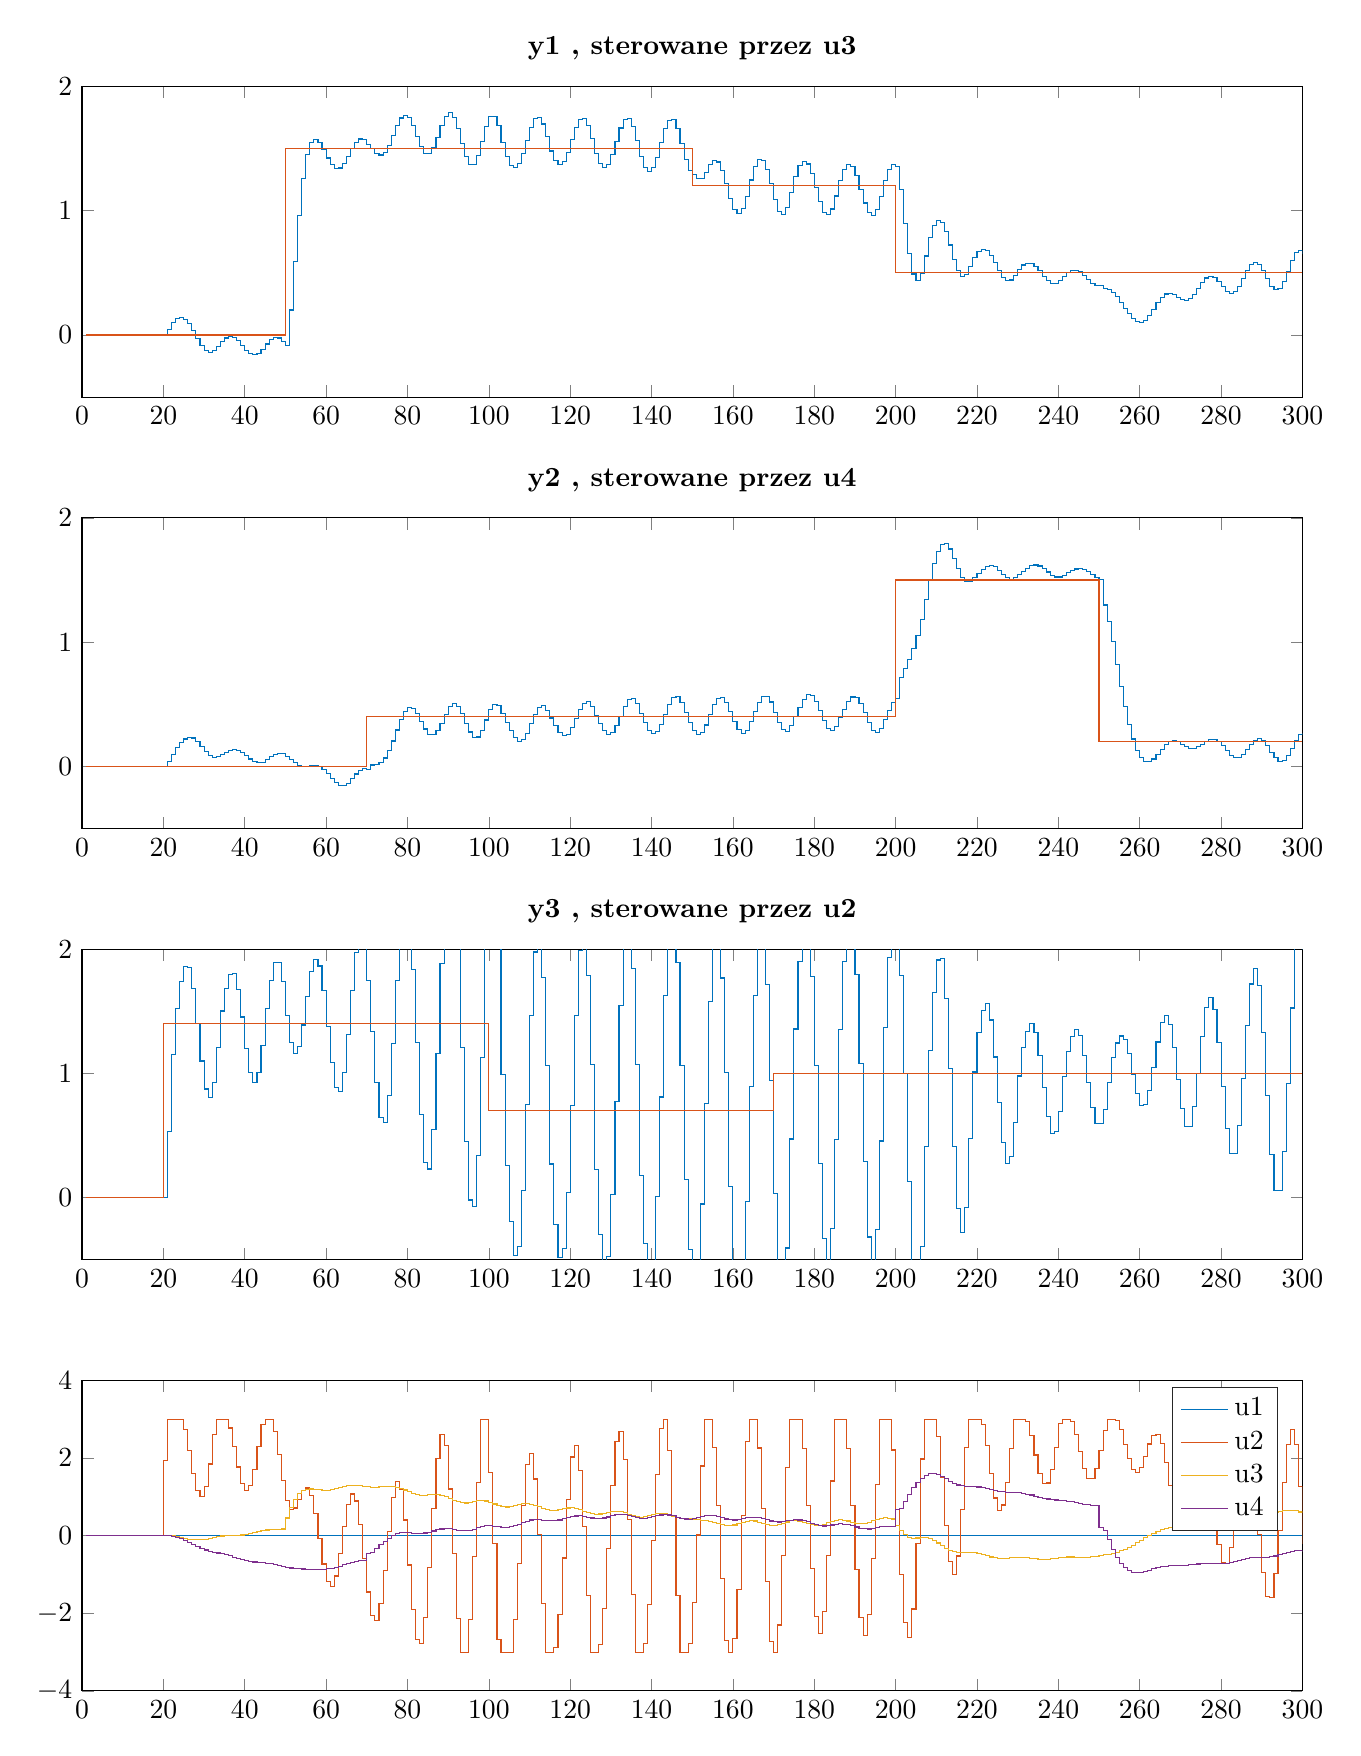
\begin{tikzpicture}

\begin{axis}[%
width=6.102in,
height=1.553in,
at={(1.024in,7.552in)},
scale only axis,
xmin=0,
xmax=300,
ymin=-0.5,
ymax=2,
axis background/.style={fill=white},
title style={font=\bfseries},
title={y1 , sterowane przez u3}
]
\addplot[const plot, color=mycolor1, forget plot] table[row sep=crcr] {%
1	0\\
2	0\\
3	0\\
4	0\\
5	0\\
6	0\\
7	0\\
8	0\\
9	0\\
10	0\\
11	0\\
12	0\\
13	0\\
14	0\\
15	0\\
16	0\\
17	0\\
18	0\\
19	0\\
20	0\\
21	0.0427356887106046\\
22	0.0996423529114932\\
23	0.133231737335584\\
24	0.13981073494923\\
25	0.124424774443444\\
26	0.0891252037271934\\
27	0.0364966285033995\\
28	-0.0249286001260704\\
29	-0.0826117183847898\\
30	-0.123776400006651\\
31	-0.139124381116757\\
32	-0.126069105732608\\
33	-0.0902420015186471\\
34	-0.0505834705027168\\
35	-0.0245687778048963\\
36	-0.0142211911257555\\
37	-0.0218076119946923\\
38	-0.0471938722950384\\
39	-0.084133246018397\\
40	-0.122231563001156\\
41	-0.150245163023737\\
42	-0.159371562231367\\
43	-0.146164385289047\\
44	-0.11403580156762\\
45	-0.0726197829488683\\
46	-0.0392553545845947\\
47	-0.0214218191283463\\
48	-0.0246041425834801\\
49	-0.0492077547713425\\
50	-0.088288376496264\\
51	0.200635312789686\\
52	0.592410762862189\\
53	0.964394331245907\\
54	1.25613968439008\\
55	1.44923480578043\\
56	1.54959134711738\\
57	1.57493981252935\\
58	1.54744382846962\\
59	1.49003341439072\\
60	1.42453925028833\\
61	1.37005534230514\\
62	1.34087825466545\\
63	1.34430569648158\\
64	1.37915226513078\\
65	1.43589937020066\\
66	1.49896553135018\\
67	1.55085155361923\\
68	1.57717055117381\\
69	1.57110445105243\\
70	1.53583219077707\\
71	1.49737758669998\\
72	1.46163574169452\\
73	1.44832637598539\\
74	1.46930123488673\\
75	1.52439944927885\\
76	1.60245288321158\\
77	1.68385836326767\\
78	1.74595517804914\\
79	1.77005904743474\\
80	1.74777794159039\\
81	1.68445841169704\\
82	1.59844099438273\\
83	1.51605813511775\\
84	1.46369685168246\\
85	1.45931016828031\\
86	1.50611096104629\\
87	1.59065573692507\\
88	1.68623803985484\\
89	1.76083304009254\\
90	1.78729169738726\\
91	1.75259126662961\\
92	1.66304589584828\\
93	1.54350129077215\\
94	1.43594068186814\\
95	1.37385486186985\\
96	1.37478178842852\\
97	1.44102972263059\\
98	1.55450952022621\\
99	1.68019130760738\\
100	1.76072536483971\\
101	1.76025465642228\\
102	1.68452721966036\\
103	1.54858314877691\\
104	1.43363344279257\\
105	1.36591615093143\\
106	1.34437585093021\\
107	1.37678703128192\\
108	1.45872187482364\\
109	1.56797181818696\\
110	1.67293209553305\\
111	1.74185619181296\\
112	1.75219682923652\\
113	1.69845921255429\\
114	1.59524136879165\\
115	1.48081017898227\\
116	1.40395633726356\\
117	1.37282872922922\\
118	1.39532596182641\\
119	1.46843954105132\\
120	1.57115231537699\\
121	1.67168002402926\\
122	1.73755714702449\\
123	1.74550423520694\\
124	1.68945362513975\\
125	1.58372446068786\\
126	1.4628609324503\\
127	1.38093703614542\\
128	1.34828930705363\\
129	1.37290619041414\\
130	1.45110761063874\\
131	1.56017946236297\\
132	1.66599673482813\\
133	1.7339816834059\\
134	1.73971755572223\\
135	1.67740114864286\\
136	1.56301975237743\\
137	1.43516919002272\\
138	1.34950494104872\\
139	1.31677490633274\\
140	1.34513926533327\\
141	1.42998450942986\\
142	1.54663349731707\\
143	1.65863437909291\\
144	1.72929396258588\\
145	1.73335310778913\\
146	1.66544882884307\\
147	1.54327098989294\\
148	1.41044238307862\\
149	1.32268781696934\\
150	1.29052608631346\\
151	1.25617734524832\\
152	1.26203158246745\\
153	1.30863650048004\\
154	1.3696968591112\\
155	1.40426134239589\\
156	1.39239241528104\\
157	1.32647993843514\\
158	1.2176182682519\\
159	1.09564928820523\\
160	1.00933145918003\\
161	0.979619779057732\\
162	1.01741281718011\\
163	1.1159644919561\\
164	1.2471750761454\\
165	1.35444779762054\\
166	1.41149598648763\\
167	1.40534443152257\\
168	1.33405057304551\\
169	1.2161819722136\\
170	1.08699005725261\\
171	0.996424849942086\\
172	0.972655428174669\\
173	1.02822934100687\\
174	1.14842060513727\\
175	1.27717569484163\\
176	1.36224552408546\\
177	1.39798325895173\\
178	1.37641008516837\\
179	1.29877340080525\\
180	1.18583289154186\\
181	1.07082123875007\\
182	0.98894938031581\\
183	0.966996400127273\\
184	1.01430759481531\\
185	1.11852481399241\\
186	1.24394045307648\\
187	1.33068029221303\\
188	1.37076729451025\\
189	1.35472160411851\\
190	1.28254174977534\\
191	1.17414193410302\\
192	1.06238608277508\\
193	0.982515125608475\\
194	0.961626069331432\\
195	1.0095410436038\\
196	1.1143929296882\\
197	1.24303286277239\\
198	1.33281810560583\\
199	1.3748361252592\\
200	1.35931116957369\\
201	1.16889557527705\\
202	0.900713830314073\\
203	0.65352188574521\\
204	0.490950453447763\\
205	0.440317925603119\\
206	0.4986028753261\\
207	0.635937890414087\\
208	0.781541877065324\\
209	0.880173459985835\\
210	0.922408128207864\\
211	0.90565437431035\\
212	0.833135121042869\\
213	0.723884399141467\\
214	0.607673254262977\\
215	0.515734873836781\\
216	0.472188849074534\\
217	0.486803693016961\\
218	0.551375912408635\\
219	0.624086095433441\\
220	0.671274180461939\\
221	0.688672122630609\\
222	0.678445636038795\\
223	0.640345309985348\\
224	0.581882758941371\\
225	0.517795233666078\\
226	0.464910323080748\\
227	0.437418138531786\\
228	0.442552507911958\\
229	0.47778711440942\\
230	0.527526524328019\\
231	0.562790320489341\\
232	0.578737126647752\\
233	0.576440110825514\\
234	0.554522785951596\\
235	0.516983531842816\\
236	0.473394074046106\\
237	0.435394918487419\\
238	0.413419449747572\\
239	0.413583415195073\\
240	0.435444734798596\\
241	0.47169373463951\\
242	0.50192821418899\\
243	0.518661222217977\\
244	0.520811100504524\\
245	0.506641197560109\\
246	0.478857580752079\\
247	0.445095447557779\\
248	0.415187968598208\\
249	0.398245225720546\\
250	0.399861143320045\\
251	0.376563171734047\\
252	0.363480577507022\\
253	0.343521810907025\\
254	0.308170621770421\\
255	0.264264652504373\\
256	0.216399524580338\\
257	0.169398551580952\\
258	0.130169684429341\\
259	0.105864417067745\\
260	0.101839668245207\\
261	0.119995074336929\\
262	0.157665149922734\\
263	0.207666431419047\\
264	0.259753129362219\\
265	0.303183427394866\\
266	0.329691879222253\\
267	0.335960510754641\\
268	0.324754701053335\\
269	0.304252447142193\\
270	0.285647284160249\\
271	0.279673340749004\\
272	0.293098519813742\\
273	0.326315047394643\\
274	0.372875678762878\\
275	0.421245603796165\\
276	0.458334117256833\\
277	0.473759589870025\\
278	0.463493119164885\\
279	0.431641958232981\\
280	0.389663788512929\\
281	0.353100723650036\\
282	0.336743398737618\\
283	0.349712313940294\\
284	0.39206993995271\\
285	0.454181425526659\\
286	0.519219318132023\\
287	0.568200370333045\\
288	0.586069022076283\\
289	0.566898571819978\\
290	0.516441893331626\\
291	0.451016330941453\\
292	0.392844237223039\\
293	0.363143513448139\\
294	0.375088387562555\\
295	0.428944896913182\\
296	0.511124721024305\\
297	0.597729686693582\\
298	0.661721632840988\\
299	0.681603079467398\\
300	0.648856448114932\\
};
\addplot[const plot, color=mycolor2, forget plot] table[row sep=crcr] {%
1	0\\
2	0\\
3	0\\
4	0\\
5	0\\
6	0\\
7	0\\
8	0\\
9	0\\
10	0\\
11	0\\
12	0\\
13	0\\
14	0\\
15	0\\
16	0\\
17	0\\
18	0\\
19	0\\
20	0\\
21	0\\
22	0\\
23	0\\
24	0\\
25	0\\
26	0\\
27	0\\
28	0\\
29	0\\
30	0\\
31	0\\
32	0\\
33	0\\
34	0\\
35	0\\
36	0\\
37	0\\
38	0\\
39	0\\
40	0\\
41	0\\
42	0\\
43	0\\
44	0\\
45	0\\
46	0\\
47	0\\
48	0\\
49	0\\
50	1.5\\
51	1.5\\
52	1.5\\
53	1.5\\
54	1.5\\
55	1.5\\
56	1.5\\
57	1.5\\
58	1.5\\
59	1.5\\
60	1.5\\
61	1.5\\
62	1.5\\
63	1.5\\
64	1.5\\
65	1.5\\
66	1.5\\
67	1.5\\
68	1.5\\
69	1.5\\
70	1.5\\
71	1.5\\
72	1.5\\
73	1.5\\
74	1.5\\
75	1.5\\
76	1.5\\
77	1.5\\
78	1.5\\
79	1.5\\
80	1.5\\
81	1.5\\
82	1.5\\
83	1.5\\
84	1.5\\
85	1.5\\
86	1.5\\
87	1.5\\
88	1.5\\
89	1.5\\
90	1.5\\
91	1.5\\
92	1.5\\
93	1.5\\
94	1.5\\
95	1.5\\
96	1.5\\
97	1.5\\
98	1.5\\
99	1.5\\
100	1.5\\
101	1.5\\
102	1.5\\
103	1.5\\
104	1.5\\
105	1.5\\
106	1.5\\
107	1.5\\
108	1.5\\
109	1.5\\
110	1.5\\
111	1.5\\
112	1.5\\
113	1.5\\
114	1.5\\
115	1.5\\
116	1.5\\
117	1.5\\
118	1.5\\
119	1.5\\
120	1.5\\
121	1.5\\
122	1.5\\
123	1.5\\
124	1.5\\
125	1.5\\
126	1.5\\
127	1.5\\
128	1.5\\
129	1.5\\
130	1.5\\
131	1.5\\
132	1.5\\
133	1.5\\
134	1.5\\
135	1.5\\
136	1.5\\
137	1.5\\
138	1.5\\
139	1.5\\
140	1.5\\
141	1.5\\
142	1.5\\
143	1.5\\
144	1.5\\
145	1.5\\
146	1.5\\
147	1.5\\
148	1.5\\
149	1.5\\
150	1.2\\
151	1.2\\
152	1.2\\
153	1.2\\
154	1.2\\
155	1.2\\
156	1.2\\
157	1.2\\
158	1.2\\
159	1.2\\
160	1.2\\
161	1.2\\
162	1.2\\
163	1.2\\
164	1.2\\
165	1.2\\
166	1.2\\
167	1.2\\
168	1.2\\
169	1.2\\
170	1.2\\
171	1.2\\
172	1.2\\
173	1.2\\
174	1.2\\
175	1.2\\
176	1.2\\
177	1.2\\
178	1.2\\
179	1.2\\
180	1.2\\
181	1.2\\
182	1.2\\
183	1.2\\
184	1.2\\
185	1.2\\
186	1.2\\
187	1.2\\
188	1.2\\
189	1.2\\
190	1.2\\
191	1.2\\
192	1.2\\
193	1.2\\
194	1.2\\
195	1.2\\
196	1.2\\
197	1.2\\
198	1.2\\
199	1.2\\
200	0.5\\
201	0.5\\
202	0.5\\
203	0.5\\
204	0.5\\
205	0.5\\
206	0.5\\
207	0.5\\
208	0.5\\
209	0.5\\
210	0.5\\
211	0.5\\
212	0.5\\
213	0.5\\
214	0.5\\
215	0.5\\
216	0.5\\
217	0.5\\
218	0.5\\
219	0.5\\
220	0.5\\
221	0.5\\
222	0.5\\
223	0.5\\
224	0.5\\
225	0.5\\
226	0.5\\
227	0.5\\
228	0.5\\
229	0.5\\
230	0.5\\
231	0.5\\
232	0.5\\
233	0.5\\
234	0.5\\
235	0.5\\
236	0.5\\
237	0.5\\
238	0.5\\
239	0.5\\
240	0.5\\
241	0.5\\
242	0.5\\
243	0.5\\
244	0.5\\
245	0.5\\
246	0.5\\
247	0.5\\
248	0.5\\
249	0.5\\
250	0.5\\
251	0.5\\
252	0.5\\
253	0.5\\
254	0.5\\
255	0.5\\
256	0.5\\
257	0.5\\
258	0.5\\
259	0.5\\
260	0.5\\
261	0.5\\
262	0.5\\
263	0.5\\
264	0.5\\
265	0.5\\
266	0.5\\
267	0.5\\
268	0.5\\
269	0.5\\
270	0.5\\
271	0.5\\
272	0.5\\
273	0.5\\
274	0.5\\
275	0.5\\
276	0.5\\
277	0.5\\
278	0.5\\
279	0.5\\
280	0.5\\
281	0.5\\
282	0.5\\
283	0.5\\
284	0.5\\
285	0.5\\
286	0.5\\
287	0.5\\
288	0.5\\
289	0.5\\
290	0.5\\
291	0.5\\
292	0.5\\
293	0.5\\
294	0.5\\
295	0.5\\
296	0.5\\
297	0.5\\
298	0.5\\
299	0.5\\
300	0.5\\
};
\end{axis}

\begin{axis}[%
width=6.102in,
height=1.553in,
at={(1.024in,5.395in)},
scale only axis,
xmin=0,
xmax=300,
ymin=-0.5,
ymax=2,
axis background/.style={fill=white},
title style={font=\bfseries},
title={y2 , sterowane przez u4}
]
\addplot[const plot, color=mycolor1, forget plot] table[row sep=crcr] {%
1	0\\
2	0\\
3	0\\
4	0\\
5	0\\
6	0\\
7	0\\
8	0\\
9	0\\
10	0\\
11	0\\
12	0\\
13	0\\
14	0\\
15	0\\
16	0\\
17	0\\
18	0\\
19	0\\
20	0\\
21	0.0394229844325725\\
22	0.099029925371794\\
23	0.149792294000774\\
24	0.190159496497694\\
25	0.220548063036863\\
26	0.234957805159333\\
27	0.228221298615249\\
28	0.201891290233015\\
29	0.162996709738131\\
30	0.121719706467291\\
31	0.0889613984572828\\
32	0.0732084348208753\\
33	0.0777570474437501\\
34	0.0937681314190743\\
35	0.110360561130889\\
36	0.125898569297771\\
37	0.134771201980869\\
38	0.131068734635916\\
39	0.114120650516032\\
40	0.0879494594116659\\
41	0.0595990653018846\\
42	0.0372548933169516\\
43	0.0276795678524574\\
44	0.0338254248428808\\
45	0.0536004495326022\\
46	0.0763609895304952\\
47	0.0966113914946444\\
48	0.10712432330711\\
49	0.102002497076856\\
50	0.0807888354430175\\
51	0.053654043222674\\
52	0.0283756146281543\\
53	0.010100359402714\\
54	0.00169668818534834\\
55	0.00196843457639263\\
56	0.00582538272640303\\
57	0.00631662932383677\\
58	-0.0027813940707242\\
59	-0.0245706792656936\\
60	-0.0575526154694467\\
61	-0.0956542975310768\\
62	-0.129860124974959\\
63	-0.150996750331761\\
64	-0.152811162813357\\
65	-0.134329895170242\\
66	-0.100656946163948\\
67	-0.0618284042074746\\
68	-0.0299595112979034\\
69	-0.0155010447891142\\
70	-0.0237727094328227\\
71	0.0106143591181108\\
72	0.0154270751555545\\
73	0.030513752258704\\
74	0.0675182540807108\\
75	0.12613117928496\\
76	0.203937071599369\\
77	0.292481365524718\\
78	0.377345271731623\\
79	0.442167503387074\\
80	0.473699347866598\\
81	0.466314651381672\\
82	0.424557601660695\\
83	0.362666919503627\\
84	0.300945722449241\\
85	0.259908468554995\\
86	0.253942520936508\\
87	0.286508496738329\\
88	0.348544967767139\\
89	0.420811131631124\\
90	0.479663166485651\\
91	0.504602842877867\\
92	0.485246541983276\\
93	0.425397505151236\\
94	0.34782961513583\\
95	0.276989776947421\\
96	0.23401231222149\\
97	0.235986329660338\\
98	0.286619132192022\\
99	0.373112966864212\\
100	0.455212280421215\\
101	0.498437379163263\\
102	0.492658767927557\\
103	0.428351612248112\\
104	0.355874995728862\\
105	0.290020188533892\\
106	0.232428756087601\\
107	0.203363703993041\\
108	0.216323446588177\\
109	0.268070158400872\\
110	0.343534668185922\\
111	0.420214927240557\\
112	0.47398158017321\\
113	0.48682554859007\\
114	0.453223453728228\\
115	0.389058046043885\\
116	0.326779068217439\\
117	0.273909367271078\\
118	0.246913488809426\\
119	0.259518192517494\\
120	0.309961590148432\\
121	0.383582453842577\\
122	0.457969904332652\\
123	0.50909968163552\\
124	0.518998253904115\\
125	0.482172483461387\\
126	0.41114040030365\\
127	0.342544314858462\\
128	0.285772182317688\\
129	0.257539221282993\\
130	0.271819397250295\\
131	0.326316686271242\\
132	0.404915569148328\\
133	0.483393541026956\\
134	0.536135564313034\\
135	0.544292137298491\\
136	0.502534869549596\\
137	0.425930337387005\\
138	0.352224299354861\\
139	0.291578230317865\\
140	0.261888495956829\\
141	0.277536987223921\\
142	0.335582727062235\\
143	0.418551471017026\\
144	0.500422487174258\\
145	0.554212379370727\\
146	0.560330636076818\\
147	0.513649771245891\\
148	0.432724714076141\\
149	0.355226811071194\\
150	0.291538990460004\\
151	0.25956730533852\\
152	0.274175876335796\\
153	0.332883944075685\\
154	0.417254435995355\\
155	0.495520958522829\\
156	0.547662310020069\\
157	0.556897583940254\\
158	0.517395802565093\\
159	0.440285290256422\\
160	0.359488619157727\\
161	0.294912184298838\\
162	0.267544135557089\\
163	0.290732712326686\\
164	0.360137202338241\\
165	0.441004257478959\\
166	0.514297919413389\\
167	0.561587481553762\\
168	0.564288467021769\\
169	0.518392070571615\\
170	0.43685865988692\\
171	0.353203653825271\\
172	0.293779978423363\\
173	0.28281821975503\\
174	0.329058135968127\\
175	0.404798086211153\\
176	0.476815987035202\\
177	0.540512259648873\\
178	0.578228937112911\\
179	0.57319006414225\\
180	0.525476597983666\\
181	0.449430055486616\\
182	0.368333158616286\\
183	0.308305483864531\\
184	0.290152146716325\\
185	0.322070713573131\\
186	0.392292816776027\\
187	0.46093500869404\\
188	0.522037558167948\\
189	0.558579198795932\\
190	0.553535771586891\\
191	0.506458549880454\\
192	0.431273277242015\\
193	0.35096508669185\\
194	0.291499049041649\\
195	0.273691517691496\\
196	0.305883099408095\\
197	0.378523965088562\\
198	0.449567060968068\\
199	0.512380955016125\\
200	0.54979361348593\\
201	0.716787376222303\\
202	0.790455321282726\\
203	0.860304195715846\\
204	0.946589982138683\\
205	1.05062046627063\\
206	1.18224475662449\\
207	1.34412576736513\\
208	1.50384024504763\\
209	1.63278133797606\\
210	1.72924116108685\\
211	1.78531173495815\\
212	1.790970602942\\
213	1.74929760442322\\
214	1.67546265129435\\
215	1.59158577018099\\
216	1.52171171713544\\
217	1.48540349075842\\
218	1.49175757333065\\
219	1.5202764777403\\
220	1.5510653748134\\
221	1.58144804036998\\
222	1.606734686503\\
223	1.61612865159131\\
224	1.60557354870397\\
225	1.5792521446853\\
226	1.5463938909929\\
227	1.51869639100242\\
228	1.50689862143461\\
229	1.51702020821223\\
230	1.54481963760588\\
231	1.57180301155469\\
232	1.59553825760419\\
233	1.61440254624917\\
234	1.62113081529675\\
235	1.61259786422139\\
236	1.59152592781037\\
237	1.56426590395291\\
238	1.53912667733211\\
239	1.52411912876121\\
240	1.52429339533766\\
241	1.53988823839286\\
242	1.5584827512141\\
243	1.57558117582955\\
244	1.58902724949815\\
245	1.59308914549551\\
246	1.58485515479529\\
247	1.56618012256\\
248	1.54223171991579\\
249	1.5200037212788\\
250	1.50635756584134\\
251	1.29922270124938\\
252	1.16248337441705\\
253	1.00275985643547\\
254	0.818906255322218\\
255	0.641114163551248\\
256	0.479727987626634\\
257	0.338079449185291\\
258	0.220190361352882\\
259	0.129669492242839\\
260	0.068929316409599\\
261	0.0387058701793318\\
262	0.0371273213576682\\
263	0.0590375765999864\\
264	0.0961779629438668\\
265	0.138357003023578\\
266	0.175402559529763\\
267	0.199401313859864\\
268	0.206558360787997\\
269	0.19805558380012\\
270	0.179552241126349\\
271	0.159377208502213\\
272	0.1458854665284\\
273	0.144753412896428\\
274	0.157059663286886\\
275	0.178799779612759\\
276	0.20206078311593\\
277	0.21755726496993\\
278	0.217770033383529\\
279	0.199685622889101\\
280	0.166204557843162\\
281	0.125665777890798\\
282	0.089519998729867\\
283	0.0687974029576855\\
284	0.0704555312377252\\
285	0.0948054780955589\\
286	0.134939868423425\\
287	0.178489208980989\\
288	0.211288892463934\\
289	0.221882303097963\\
290	0.205437958704364\\
291	0.165755373507587\\
292	0.114573257374122\\
293	0.0682272064829322\\
294	0.0425779114031747\\
295	0.0477605836795954\\
296	0.0844685009927205\\
297	0.143093739331231\\
298	0.206197527803562\\
299	0.25371999926134\\
300	0.26939949237706\\
};
\addplot[const plot, color=mycolor2, forget plot] table[row sep=crcr] {%
1	0\\
2	0\\
3	0\\
4	0\\
5	0\\
6	0\\
7	0\\
8	0\\
9	0\\
10	0\\
11	0\\
12	0\\
13	0\\
14	0\\
15	0\\
16	0\\
17	0\\
18	0\\
19	0\\
20	0\\
21	0\\
22	0\\
23	0\\
24	0\\
25	0\\
26	0\\
27	0\\
28	0\\
29	0\\
30	0\\
31	0\\
32	0\\
33	0\\
34	0\\
35	0\\
36	0\\
37	0\\
38	0\\
39	0\\
40	0\\
41	0\\
42	0\\
43	0\\
44	0\\
45	0\\
46	0\\
47	0\\
48	0\\
49	0\\
50	0\\
51	0\\
52	0\\
53	0\\
54	0\\
55	0\\
56	0\\
57	0\\
58	0\\
59	0\\
60	0\\
61	0\\
62	0\\
63	0\\
64	0\\
65	0\\
66	0\\
67	0\\
68	0\\
69	0\\
70	0.4\\
71	0.4\\
72	0.4\\
73	0.4\\
74	0.4\\
75	0.4\\
76	0.4\\
77	0.4\\
78	0.4\\
79	0.4\\
80	0.4\\
81	0.4\\
82	0.4\\
83	0.4\\
84	0.4\\
85	0.4\\
86	0.4\\
87	0.4\\
88	0.4\\
89	0.4\\
90	0.4\\
91	0.4\\
92	0.4\\
93	0.4\\
94	0.4\\
95	0.4\\
96	0.4\\
97	0.4\\
98	0.4\\
99	0.4\\
100	0.4\\
101	0.4\\
102	0.4\\
103	0.4\\
104	0.4\\
105	0.4\\
106	0.4\\
107	0.4\\
108	0.4\\
109	0.4\\
110	0.4\\
111	0.4\\
112	0.4\\
113	0.4\\
114	0.4\\
115	0.4\\
116	0.4\\
117	0.4\\
118	0.4\\
119	0.4\\
120	0.4\\
121	0.4\\
122	0.4\\
123	0.4\\
124	0.4\\
125	0.4\\
126	0.4\\
127	0.4\\
128	0.4\\
129	0.4\\
130	0.4\\
131	0.4\\
132	0.4\\
133	0.4\\
134	0.4\\
135	0.4\\
136	0.4\\
137	0.4\\
138	0.4\\
139	0.4\\
140	0.4\\
141	0.4\\
142	0.4\\
143	0.4\\
144	0.4\\
145	0.4\\
146	0.4\\
147	0.4\\
148	0.4\\
149	0.4\\
150	0.4\\
151	0.4\\
152	0.4\\
153	0.4\\
154	0.4\\
155	0.4\\
156	0.4\\
157	0.4\\
158	0.4\\
159	0.4\\
160	0.4\\
161	0.4\\
162	0.4\\
163	0.4\\
164	0.4\\
165	0.4\\
166	0.4\\
167	0.4\\
168	0.4\\
169	0.4\\
170	0.4\\
171	0.4\\
172	0.4\\
173	0.4\\
174	0.4\\
175	0.4\\
176	0.4\\
177	0.4\\
178	0.4\\
179	0.4\\
180	0.4\\
181	0.4\\
182	0.4\\
183	0.4\\
184	0.4\\
185	0.4\\
186	0.4\\
187	0.4\\
188	0.4\\
189	0.4\\
190	0.4\\
191	0.4\\
192	0.4\\
193	0.4\\
194	0.4\\
195	0.4\\
196	0.4\\
197	0.4\\
198	0.4\\
199	0.4\\
200	1.5\\
201	1.5\\
202	1.5\\
203	1.5\\
204	1.5\\
205	1.5\\
206	1.5\\
207	1.5\\
208	1.5\\
209	1.5\\
210	1.5\\
211	1.5\\
212	1.5\\
213	1.5\\
214	1.5\\
215	1.5\\
216	1.5\\
217	1.5\\
218	1.5\\
219	1.5\\
220	1.5\\
221	1.5\\
222	1.5\\
223	1.5\\
224	1.5\\
225	1.5\\
226	1.5\\
227	1.5\\
228	1.5\\
229	1.5\\
230	1.5\\
231	1.5\\
232	1.5\\
233	1.5\\
234	1.5\\
235	1.5\\
236	1.5\\
237	1.5\\
238	1.5\\
239	1.5\\
240	1.5\\
241	1.5\\
242	1.5\\
243	1.5\\
244	1.5\\
245	1.5\\
246	1.5\\
247	1.5\\
248	1.5\\
249	1.5\\
250	0.2\\
251	0.2\\
252	0.2\\
253	0.2\\
254	0.2\\
255	0.2\\
256	0.2\\
257	0.2\\
258	0.2\\
259	0.2\\
260	0.2\\
261	0.2\\
262	0.2\\
263	0.2\\
264	0.2\\
265	0.2\\
266	0.2\\
267	0.2\\
268	0.2\\
269	0.2\\
270	0.2\\
271	0.2\\
272	0.2\\
273	0.2\\
274	0.2\\
275	0.2\\
276	0.2\\
277	0.2\\
278	0.2\\
279	0.2\\
280	0.2\\
281	0.2\\
282	0.2\\
283	0.2\\
284	0.2\\
285	0.2\\
286	0.2\\
287	0.2\\
288	0.2\\
289	0.2\\
290	0.2\\
291	0.2\\
292	0.2\\
293	0.2\\
294	0.2\\
295	0.2\\
296	0.2\\
297	0.2\\
298	0.2\\
299	0.2\\
300	0.2\\
};
\end{axis}

\begin{axis}[%
width=6.102in,
height=1.553in,
at={(1.024in,3.239in)},
scale only axis,
xmin=0,
xmax=300,
ymin=-0.5,
ymax=2,
axis background/.style={fill=white},
title style={font=\bfseries},
title={y3 , sterowane przez u2}
]
\addplot[const plot, color=mycolor1, forget plot] table[row sep=crcr] {%
1	0\\
2	0\\
3	0\\
4	0\\
5	0\\
6	0\\
7	0\\
8	0\\
9	0\\
10	0\\
11	0\\
12	0\\
13	0\\
14	0\\
15	0\\
16	0\\
17	0\\
18	0\\
19	0\\
20	0\\
21	0.532127935804634\\
22	1.14903752255858\\
23	1.51996945766859\\
24	1.73747610187465\\
25	1.85879217891158\\
26	1.84896775476135\\
27	1.68048737083064\\
28	1.40075483308903\\
29	1.09900481038602\\
30	0.873508634392522\\
31	0.804130618671082\\
32	0.925250036357492\\
33	1.21071283597997\\
34	1.50154965181722\\
35	1.68258036842564\\
36	1.79504419768483\\
37	1.80163865205181\\
38	1.67615906117651\\
39	1.45309060701352\\
40	1.20214958598563\\
41	1.00376399542146\\
42	0.926676598784127\\
43	1.00474572000967\\
44	1.22294655431725\\
45	1.51909445992512\\
46	1.74894589216392\\
47	1.89181891612016\\
48	1.8953556771218\\
49	1.73983616889426\\
50	1.46695706642664\\
51	1.25116915831537\\
52	1.16232229183176\\
53	1.21565053670371\\
54	1.38916498966925\\
55	1.61953300311569\\
56	1.82155181206875\\
57	1.91781518131236\\
58	1.86426425437248\\
59	1.66570621564887\\
60	1.37659123267414\\
61	1.08564002567294\\
62	0.888360043271158\\
63	0.855754163091541\\
64	1.00920290662607\\
65	1.31011077321118\\
66	1.66864467339339\\
67	1.96992112831754\\
68	2.11017018516639\\
69	2.03164186357744\\
70	1.74469540151591\\
71	1.33548308825588\\
72	0.924599081662919\\
73	0.647220495612345\\
74	0.603284577150656\\
75	0.820742650891634\\
76	1.24363588184181\\
77	1.74499300294823\\
78	2.16358704481127\\
79	2.35479616812985\\
80	2.2393574982255\\
81	1.83378583705005\\
82	1.25132699868384\\
83	0.671173249655376\\
84	0.283933650368008\\
85	0.229704615025583\\
86	0.548608009455141\\
87	1.1608888211573\\
88	1.8850894038373\\
89	2.49087079752765\\
90	2.77143435669133\\
91	2.61304952261954\\
92	2.03864216796657\\
93	1.20938412414776\\
94	0.450176654799709\\
95	-0.0193859958657123\\
96	-0.075213869492442\\
97	0.34091683110081\\
98	1.13016714843556\\
99	2.05550934730718\\
100	2.6198173684034\\
101	2.57616342768901\\
102	2.02716298459303\\
103	0.992230380264485\\
104	0.26130583498686\\
105	-0.189847038571485\\
106	-0.463732394391575\\
107	-0.39220528633868\\
108	0.0578082365260069\\
109	0.748665064163771\\
110	1.46557925591245\\
111	1.97691456679774\\
112	2.10063337758094\\
113	1.76939557622759\\
114	1.06144117611281\\
115	0.270572573399581\\
116	-0.219338907828012\\
117	-0.485215124916882\\
118	-0.410681541508358\\
119	0.0411704688529442\\
120	0.73985431579247\\
121	1.46703261846347\\
122	1.98726788212493\\
123	2.11622092287075\\
124	1.78496181476886\\
125	1.07155397814675\\
126	0.224348507001663\\
127	-0.299824476299911\\
128	-0.569653389403717\\
129	-0.473732506524661\\
130	0.0214438711067708\\
131	0.773813442565977\\
132	1.54777627638857\\
133	2.092042216313\\
134	2.21301723514077\\
135	1.84233064365656\\
136	1.06894548873815\\
137	0.17754713551153\\
138	-0.372306585806091\\
139	-0.648096562008864\\
140	-0.531950941916663\\
141	0.00569521257389714\\
142	0.809714818737909\\
143	1.62808901889281\\
144	2.19290076198646\\
145	2.30407900005409\\
146	1.89443866500463\\
147	1.06350136577005\\
148	0.144518422370393\\
149	-0.420685456161988\\
150	-0.700821481080799\\
151	-0.58864504389789\\
152	-0.0519438133500562\\
153	0.758205474157181\\
154	1.57656572626902\\
155	2.06442316516757\\
156	2.14611118372822\\
157	1.7669915800822\\
158	1.00587158876029\\
159	0.0903511235631449\\
160	-0.557432495669258\\
161	-0.853414645652854\\
162	-0.677795262893985\\
163	-0.0335582369815863\\
164	0.896140373645164\\
165	1.62716598918112\\
166	2.07089631751851\\
167	2.12749805297532\\
168	1.71804878415227\\
169	0.940303800990432\\
170	0.031551360677063\\
171	-0.602410282584871\\
172	-0.792054188082011\\
173	-0.405968352186338\\
174	0.471596287919821\\
175	1.35695911030598\\
176	1.90035042461931\\
177	2.22825060819565\\
178	2.21117057434826\\
179	1.78127438023832\\
180	1.06015030793484\\
181	0.272592828885958\\
182	-0.328673427357279\\
183	-0.534013603560845\\
184	-0.248735176052021\\
185	0.466519093204263\\
186	1.35310724160432\\
187	1.89943941533099\\
188	2.23161005344659\\
189	2.22044069727428\\
190	1.79594573002581\\
191	1.07752766239669\\
192	0.288784530272557\\
193	-0.317600148376935\\
194	-0.530772425370344\\
195	-0.253820020013799\\
196	0.455166686984801\\
197	1.36685598952739\\
198	1.92943368354117\\
199	2.2679283890567\\
200	2.25336778002742\\
201	1.79033868280852\\
202	0.99639748858254\\
203	0.130401396316589\\
204	-0.522078987888698\\
205	-0.730724066114593\\
206	-0.394704454086016\\
207	0.412779357893919\\
208	1.18648733727134\\
209	1.64893520156431\\
210	1.91255020226426\\
211	1.92210648791271\\
212	1.60471626312363\\
213	1.04160654980409\\
214	0.409813973061049\\
215	-0.0876712489684487\\
216	-0.278287363095817\\
217	-0.0771917919760193\\
218	0.47727508666568\\
219	1.01055565758211\\
220	1.32561610215711\\
221	1.50462353235635\\
222	1.56215564543064\\
223	1.42968285570179\\
224	1.13142026093972\\
225	0.762668852743965\\
226	0.440916934340952\\
227	0.274625857551431\\
228	0.329652646442106\\
229	0.603482125170266\\
230	0.978651510283205\\
231	1.20536503647692\\
232	1.33938199334716\\
233	1.39960516262924\\
234	1.33058635890901\\
235	1.13999308289828\\
236	0.888532421909053\\
237	0.655616371609253\\
238	0.518612850896994\\
239	0.529505789675486\\
240	0.695167199258174\\
241	0.971856813228011\\
242	1.17502773403619\\
243	1.29989692775648\\
244	1.35557229961079\\
245	1.30158500369385\\
246	1.14222192030824\\
247	0.926650581576832\\
248	0.722749675410484\\
249	0.597933241338731\\
250	0.598727386818861\\
251	0.712347156926121\\
252	0.925551510451817\\
253	1.12765901454746\\
254	1.24419093907231\\
255	1.30065407062748\\
256	1.27176042003147\\
257	1.15640175407507\\
258	0.993347480602946\\
259	0.837938244950789\\
260	0.74423168781024\\
261	0.749152615014652\\
262	0.859051374657731\\
263	1.04536264570659\\
264	1.25186015388919\\
265	1.41147372105887\\
266	1.46773597642658\\
267	1.39417230876345\\
268	1.2051127871807\\
269	0.953787806671567\\
270	0.717486872082889\\
271	0.573798286128556\\
272	0.575146472169371\\
273	0.729885764572513\\
274	0.99660626456761\\
275	1.29440902437188\\
276	1.52684284557284\\
277	1.61255019550786\\
278	1.51299979555385\\
279	1.2479977659285\\
280	0.893063843716883\\
281	0.55832415544531\\
282	0.354623268677291\\
283	0.357139422467769\\
284	0.57829409945416\\
285	0.959479776875631\\
286	1.38558087609622\\
287	1.71903715042335\\
288	1.84355884907813\\
289	1.70377037370819\\
290	1.32748090900545\\
291	0.822102151541845\\
292	0.34466391404472\\
293	0.0535191582462698\\
294	0.0563884283404157\\
295	0.371575146107659\\
296	0.915978513793833\\
297	1.52563342206218\\
298	2.00419896092646\\
299	2.18532569956627\\
300	1.98933083862569\\
};
\addplot[const plot, color=mycolor2, forget plot] table[row sep=crcr] {%
1	0\\
2	0\\
3	0\\
4	0\\
5	0\\
6	0\\
7	0\\
8	0\\
9	0\\
10	0\\
11	0\\
12	0\\
13	0\\
14	0\\
15	0\\
16	0\\
17	0\\
18	0\\
19	0\\
20	1.4\\
21	1.4\\
22	1.4\\
23	1.4\\
24	1.4\\
25	1.4\\
26	1.4\\
27	1.4\\
28	1.4\\
29	1.4\\
30	1.4\\
31	1.4\\
32	1.4\\
33	1.4\\
34	1.4\\
35	1.4\\
36	1.4\\
37	1.4\\
38	1.4\\
39	1.4\\
40	1.4\\
41	1.4\\
42	1.4\\
43	1.4\\
44	1.4\\
45	1.4\\
46	1.4\\
47	1.4\\
48	1.4\\
49	1.4\\
50	1.4\\
51	1.4\\
52	1.4\\
53	1.4\\
54	1.4\\
55	1.4\\
56	1.4\\
57	1.4\\
58	1.4\\
59	1.4\\
60	1.4\\
61	1.4\\
62	1.4\\
63	1.4\\
64	1.4\\
65	1.4\\
66	1.4\\
67	1.4\\
68	1.4\\
69	1.4\\
70	1.4\\
71	1.4\\
72	1.4\\
73	1.4\\
74	1.4\\
75	1.4\\
76	1.4\\
77	1.4\\
78	1.4\\
79	1.4\\
80	1.4\\
81	1.4\\
82	1.4\\
83	1.4\\
84	1.4\\
85	1.4\\
86	1.4\\
87	1.4\\
88	1.4\\
89	1.4\\
90	1.4\\
91	1.4\\
92	1.4\\
93	1.4\\
94	1.4\\
95	1.4\\
96	1.4\\
97	1.4\\
98	1.4\\
99	1.4\\
100	0.7\\
101	0.7\\
102	0.7\\
103	0.7\\
104	0.7\\
105	0.7\\
106	0.7\\
107	0.7\\
108	0.7\\
109	0.7\\
110	0.7\\
111	0.7\\
112	0.7\\
113	0.7\\
114	0.7\\
115	0.7\\
116	0.7\\
117	0.7\\
118	0.7\\
119	0.7\\
120	0.7\\
121	0.7\\
122	0.7\\
123	0.7\\
124	0.7\\
125	0.7\\
126	0.7\\
127	0.7\\
128	0.7\\
129	0.7\\
130	0.7\\
131	0.7\\
132	0.7\\
133	0.7\\
134	0.7\\
135	0.7\\
136	0.7\\
137	0.7\\
138	0.7\\
139	0.7\\
140	0.7\\
141	0.7\\
142	0.7\\
143	0.7\\
144	0.7\\
145	0.7\\
146	0.7\\
147	0.7\\
148	0.7\\
149	0.7\\
150	0.7\\
151	0.7\\
152	0.7\\
153	0.7\\
154	0.7\\
155	0.7\\
156	0.7\\
157	0.7\\
158	0.7\\
159	0.7\\
160	0.7\\
161	0.7\\
162	0.7\\
163	0.7\\
164	0.7\\
165	0.7\\
166	0.7\\
167	0.7\\
168	0.7\\
169	0.7\\
170	1\\
171	1\\
172	1\\
173	1\\
174	1\\
175	1\\
176	1\\
177	1\\
178	1\\
179	1\\
180	1\\
181	1\\
182	1\\
183	1\\
184	1\\
185	1\\
186	1\\
187	1\\
188	1\\
189	1\\
190	1\\
191	1\\
192	1\\
193	1\\
194	1\\
195	1\\
196	1\\
197	1\\
198	1\\
199	1\\
200	1\\
201	1\\
202	1\\
203	1\\
204	1\\
205	1\\
206	1\\
207	1\\
208	1\\
209	1\\
210	1\\
211	1\\
212	1\\
213	1\\
214	1\\
215	1\\
216	1\\
217	1\\
218	1\\
219	1\\
220	1\\
221	1\\
222	1\\
223	1\\
224	1\\
225	1\\
226	1\\
227	1\\
228	1\\
229	1\\
230	1\\
231	1\\
232	1\\
233	1\\
234	1\\
235	1\\
236	1\\
237	1\\
238	1\\
239	1\\
240	1\\
241	1\\
242	1\\
243	1\\
244	1\\
245	1\\
246	1\\
247	1\\
248	1\\
249	1\\
250	1\\
251	1\\
252	1\\
253	1\\
254	1\\
255	1\\
256	1\\
257	1\\
258	1\\
259	1\\
260	1\\
261	1\\
262	1\\
263	1\\
264	1\\
265	1\\
266	1\\
267	1\\
268	1\\
269	1\\
270	1\\
271	1\\
272	1\\
273	1\\
274	1\\
275	1\\
276	1\\
277	1\\
278	1\\
279	1\\
280	1\\
281	1\\
282	1\\
283	1\\
284	1\\
285	1\\
286	1\\
287	1\\
288	1\\
289	1\\
290	1\\
291	1\\
292	1\\
293	1\\
294	1\\
295	1\\
296	1\\
297	1\\
298	1\\
299	1\\
300	1\\
};
\end{axis}

\begin{axis}[%
width=6.102in,
height=1.553in,
at={(1.024in,1.083in)},
scale only axis,
xmin=0,
xmax=300,
ymin=-4,
ymax=4,
axis background/.style={fill=white},
legend style={legend cell align=left, align=left, draw=white!15!black}
]
\addplot[const plot, color=mycolor1] table[row sep=crcr] {%
1	0\\
2	0\\
3	0\\
4	0\\
5	0\\
6	0\\
7	0\\
8	0\\
9	0\\
10	0\\
11	0\\
12	0\\
13	0\\
14	0\\
15	0\\
16	0\\
17	0\\
18	0\\
19	0\\
20	0\\
21	0\\
22	0\\
23	0\\
24	0\\
25	0\\
26	0\\
27	0\\
28	0\\
29	0\\
30	0\\
31	0\\
32	0\\
33	0\\
34	0\\
35	0\\
36	0\\
37	0\\
38	0\\
39	0\\
40	0\\
41	0\\
42	0\\
43	0\\
44	0\\
45	0\\
46	0\\
47	0\\
48	0\\
49	0\\
50	0\\
51	0\\
52	0\\
53	0\\
54	0\\
55	0\\
56	0\\
57	0\\
58	0\\
59	0\\
60	0\\
61	0\\
62	0\\
63	0\\
64	0\\
65	0\\
66	0\\
67	0\\
68	0\\
69	0\\
70	0\\
71	0\\
72	0\\
73	0\\
74	0\\
75	0\\
76	0\\
77	0\\
78	0\\
79	0\\
80	0\\
81	0\\
82	0\\
83	0\\
84	0\\
85	0\\
86	0\\
87	0\\
88	0\\
89	0\\
90	0\\
91	0\\
92	0\\
93	0\\
94	0\\
95	0\\
96	0\\
97	0\\
98	0\\
99	0\\
100	0\\
101	0\\
102	0\\
103	0\\
104	0\\
105	0\\
106	0\\
107	0\\
108	0\\
109	0\\
110	0\\
111	0\\
112	0\\
113	0\\
114	0\\
115	0\\
116	0\\
117	0\\
118	0\\
119	0\\
120	0\\
121	0\\
122	0\\
123	0\\
124	0\\
125	0\\
126	0\\
127	0\\
128	0\\
129	0\\
130	0\\
131	0\\
132	0\\
133	0\\
134	0\\
135	0\\
136	0\\
137	0\\
138	0\\
139	0\\
140	0\\
141	0\\
142	0\\
143	0\\
144	0\\
145	0\\
146	0\\
147	0\\
148	0\\
149	0\\
150	0\\
151	0\\
152	0\\
153	0\\
154	0\\
155	0\\
156	0\\
157	0\\
158	0\\
159	0\\
160	0\\
161	0\\
162	0\\
163	0\\
164	0\\
165	0\\
166	0\\
167	0\\
168	0\\
169	0\\
170	0\\
171	0\\
172	0\\
173	0\\
174	0\\
175	0\\
176	0\\
177	0\\
178	0\\
179	0\\
180	0\\
181	0\\
182	0\\
183	0\\
184	0\\
185	0\\
186	0\\
187	0\\
188	0\\
189	0\\
190	0\\
191	0\\
192	0\\
193	0\\
194	0\\
195	0\\
196	0\\
197	0\\
198	0\\
199	0\\
200	0\\
201	0\\
202	0\\
203	0\\
204	0\\
205	0\\
206	0\\
207	0\\
208	0\\
209	0\\
210	0\\
211	0\\
212	0\\
213	0\\
214	0\\
215	0\\
216	0\\
217	0\\
218	0\\
219	0\\
220	0\\
221	0\\
222	0\\
223	0\\
224	0\\
225	0\\
226	0\\
227	0\\
228	0\\
229	0\\
230	0\\
231	0\\
232	0\\
233	0\\
234	0\\
235	0\\
236	0\\
237	0\\
238	0\\
239	0\\
240	0\\
241	0\\
242	0\\
243	0\\
244	0\\
245	0\\
246	0\\
247	0\\
248	0\\
249	0\\
250	0\\
251	0\\
252	0\\
253	0\\
254	0\\
255	0\\
256	0\\
257	0\\
258	0\\
259	0\\
260	0\\
261	0\\
262	0\\
263	0\\
264	0\\
265	0\\
266	0\\
267	0\\
268	0\\
269	0\\
270	0\\
271	0\\
272	0\\
273	0\\
274	0\\
275	0\\
276	0\\
277	0\\
278	0\\
279	0\\
280	0\\
281	0\\
282	0\\
283	0\\
284	0\\
285	0\\
286	0\\
287	0\\
288	0\\
289	0\\
290	0\\
291	0\\
292	0\\
293	0\\
294	0\\
295	0\\
296	0\\
297	0\\
298	0\\
299	0\\
300	0\\
};
\addlegendentry{u1}

\addplot[const plot, color=mycolor2] table[row sep=crcr] {%
1	0\\
2	0\\
3	0\\
4	0\\
5	0\\
6	0\\
7	0\\
8	0\\
9	0\\
10	0\\
11	0\\
12	0\\
13	0\\
14	0\\
15	0\\
16	0\\
17	0\\
18	0\\
19	0\\
20	1.932\\
21	3\\
22	3\\
23	3\\
24	3\\
25	2.74244580555877\\
26	2.19931945295947\\
27	1.59747853614157\\
28	1.1506351793338\\
29	1.01484679481284\\
30	1.26229005386448\\
31	1.84391754753467\\
32	2.59409855204538\\
33	3\\
34	3\\
35	3\\
36	2.7723552228569\\
37	2.30190301580581\\
38	1.76771466980765\\
39	1.34237519975804\\
40	1.16068332021301\\
41	1.29350494621343\\
42	1.7134880695968\\
43	2.29519132948563\\
44	2.8511886060358\\
45	3\\
46	2.98781655936982\\
47	2.66966863635731\\
48	2.08699588439511\\
49	1.43011059440635\\
50	0.903816056678641\\
51	0.677323259806042\\
52	0.710947511879059\\
53	0.927329705286624\\
54	1.15694516972553\\
55	1.22601636650068\\
56	1.02846969522005\\
57	0.558605042259142\\
58	-0.0853548400283274\\
59	-0.730419311273672\\
60	-1.18493615555774\\
61	-1.30365162576009\\
62	-1.04049479889449\\
63	-0.471279185890155\\
64	0.222808874409907\\
65	0.807854835587169\\
66	1.07086686588134\\
67	0.891468643764175\\
68	0.287860465988087\\
69	-0.579799051985148\\
70	-1.45253581183267\\
71	-2.05112948250729\\
72	-2.17562746971923\\
73	-1.75735956096078\\
74	-0.908006138661148\\
75	0.11536753376712\\
76	0.983986975201574\\
77	1.39975518439747\\
78	1.19616447307801\\
79	0.401829463548521\\
80	-0.756263268730203\\
81	-1.91442668246582\\
82	-2.68303723932456\\
83	-2.77326579465953\\
84	-2.09911942204574\\
85	-0.819580898929311\\
86	0.697010934718802\\
87	1.97982990666218\\
88	2.60331240898822\\
89	2.32995086017516\\
90	1.20085878073453\\
91	-0.459156290988617\\
92	-2.12939861950834\\
93	-3\\
94	-3\\
95	-2.16392470481262\\
96	-0.546717710702729\\
97	1.37766615830147\\
98	2.98272987154541\\
99	3\\
100	1.63532723330467\\
101	-0.20147653744591\\
102	-2.68237533920741\\
103	-3\\
104	-3\\
105	-3\\
106	-2.15792251413635\\
107	-0.715881889382404\\
108	0.766678079599909\\
109	1.8268836123864\\
110	2.10679694917608\\
111	1.45897186489991\\
112	0.0351087670587447\\
113	-1.74419385548751\\
114	-3\\
115	-3\\
116	-2.87553573249383\\
117	-2.02983791012706\\
118	-0.577867257538954\\
119	0.937573354479284\\
120	2.02476004248834\\
121	2.31993183664916\\
122	1.67585461343819\\
123	0.243688003492763\\
124	-1.55302785772699\\
125	-3\\
126	-3\\
127	-2.81623211901317\\
128	-1.88771944524654\\
129	-0.330122620694369\\
130	1.28008929717583\\
131	2.41489718555887\\
132	2.69156719686387\\
133	1.96420006521526\\
134	0.405826353830244\\
135	-1.52262293266692\\
136	-3\\
137	-3\\
138	-2.78731959860554\\
139	-1.77968117839049\\
140	-0.120543365312099\\
141	1.5758465362523\\
142	2.75150862798564\\
143	3\\
144	2.18848313937778\\
145	0.507933925662265\\
146	-1.54595613999457\\
147	-3\\
148	-3\\
149	-2.77561796630429\\
150	-1.71380401352499\\
151	0.0146895579865214\\
152	1.79303668134402\\
153	3\\
154	3\\
155	2.26944421335424\\
156	0.772368509537819\\
157	-1.0942812404881\\
158	-2.69125015191253\\
159	-3\\
160	-2.65206113596152\\
161	-1.39295870588381\\
162	0.512975233058\\
163	2.42315316333988\\
164	3\\
165	3\\
166	2.25479325646869\\
167	0.69031178891298\\
168	-1.17790488529275\\
169	-2.72015093250583\\
170	-3\\
171	-2.3030243237503\\
172	-0.520735761252447\\
173	1.76421126625375\\
174	3\\
175	3\\
176	3\\
177	2.24589901422033\\
178	0.768905912544013\\
179	-0.853159442894265\\
180	-2.08690657685337\\
181	-2.52160464389801\\
182	-1.9576752280949\\
183	-0.509351525237498\\
184	1.4062683052134\\
185	3\\
186	3\\
187	3\\
188	2.24835362689075\\
189	0.768598327530744\\
190	-0.864100658251985\\
191	-2.1156602630639\\
192	-2.57285890512352\\
193	-2.03173571696472\\
194	-0.601347535111739\\
195	1.30539962251487\\
196	3\\
197	3\\
198	2.98451075621319\\
199	2.20488313570864\\
200	0.681156533193721\\
201	-0.997545586621599\\
202	-2.24735346791821\\
203	-2.61504010243048\\
204	-1.89092644451286\\
205	-0.205703264144022\\
206	1.97385719511759\\
207	3\\
208	3\\
209	3\\
210	2.54631572899515\\
211	1.48659294425853\\
212	0.262748967087249\\
213	-0.676678483183812\\
214	-0.997095608361748\\
215	-0.525497505154207\\
216	0.667235595609099\\
217	2.26330157333984\\
218	3\\
219	3\\
220	3\\
221	2.86935144266319\\
222	2.32293330249757\\
223	1.59400814604007\\
224	0.968106395564486\\
225	0.655700818946146\\
226	0.788489813989465\\
227	1.36725333735222\\
228	2.24230847076852\\
229	3\\
230	3\\
231	3\\
232	2.94425969949563\\
233	2.58729686001556\\
234	2.07552607050768\\
235	1.607498177267\\
236	1.33322607756615\\
237	1.35589619977743\\
238	1.69364531973404\\
239	2.2595359907232\\
240	2.88438234643603\\
241	3\\
242	3\\
243	2.92785267782459\\
244	2.61489414192121\\
245	2.16313825335972\\
246	1.73768749542149\\
247	1.47283866740269\\
248	1.46137638435831\\
249	1.72344095926378\\
250	2.18922258146726\\
251	2.71633693825353\\
252	3\\
253	3\\
254	2.96068699078571\\
255	2.72964891557762\\
256	2.35536254013793\\
257	1.9781325509523\\
258	1.71235068956732\\
259	1.6335477562724\\
260	1.76015871648469\\
261	2.03932085652117\\
262	2.35995851097939\\
263	2.58752185647261\\
264	2.60777449622443\\
265	2.36655072900187\\
266	1.89239228038349\\
267	1.29330792668955\\
268	0.726979176645424\\
269	0.352484652686561\\
270	0.278208232068466\\
271	0.52282682348801\\
272	1.00310620322745\\
273	1.55433512572569\\
274	1.97888410557979\\
275	2.10882474416967\\
276	1.86297983878542\\
277	1.27928928485284\\
278	0.51020916630383\\
279	-0.219812165060418\\
280	-0.683339297480613\\
281	-0.724528351496542\\
282	-0.315143700584066\\
283	0.427633477024891\\
284	1.27000574971728\\
285	1.9306128540487\\
286	2.16982827621766\\
287	1.87130050043269\\
288	1.08842018724926\\
289	0.03809828206693\\
290	-0.959618876346883\\
291	-1.57986806084135\\
292	-1.59944041787139\\
293	-0.976956131916293\\
294	0.121364817520213\\
295	1.36243963394182\\
296	2.34462088296889\\
297	2.72509354706082\\
298	2.33644402357146\\
299	1.25336639180649\\
300	-0.215747625587575\\
};
\addlegendentry{u2}

\addplot[const plot, color=mycolor3] table[row sep=crcr] {%
1	0\\
2	0\\
3	0\\
4	0\\
5	0\\
6	0\\
7	0\\
8	0\\
9	0\\
10	0\\
11	0\\
12	0\\
13	0\\
14	0\\
15	0\\
16	0\\
17	0\\
18	0\\
19	0\\
20	0\\
21	0\\
22	-0.00783487626361084\\
23	-0.0253903794855412\\
24	-0.0481554921152067\\
25	-0.0715669312336392\\
26	-0.0920479609657835\\
27	-0.106313835408378\\
28	-0.111519463905215\\
29	-0.106340943407045\\
30	-0.0916109383719351\\
31	-0.0702954603437955\\
32	-0.0468522638058342\\
33	-0.0260583341068021\\
34	-0.0116151189239269\\
35	-0.00384551602373962\\
36	-0.000184297934553912\\
37	0.00201344080841966\\
38	0.00577448315535066\\
39	0.0140632328761962\\
40	0.0287010967746516\\
41	0.0497079958912237\\
42	0.0752157497288896\\
43	0.101929783420911\\
44	0.126070394686714\\
45	0.144540885219293\\
46	0.155953915400459\\
47	0.16194040069182\\
48	0.16521347828894\\
49	0.169367207443773\\
50	0.452978560108794\\
51	0.718344633220253\\
52	0.93009001960054\\
53	1.0748253016223\\
54	1.15789318694159\\
55	1.19367415032417\\
56	1.19891676400426\\
57	1.18897893046241\\
58	1.17606648728399\\
59	1.16861744894005\\
60	1.17123538677625\\
61	1.18490374779656\\
62	1.20746925587876\\
63	1.23447583156185\\
64	1.26036775811798\\
65	1.2799282711187\\
66	1.28966592433409\\
67	1.2887872330899\\
68	1.27944720711555\\
69	1.26614679862733\\
70	1.25439715845395\\
71	1.24901299766236\\
72	1.25009097661365\\
73	1.25708071708132\\
74	1.26591481051224\\
75	1.27068169038277\\
76	1.26569681192975\\
77	1.24732044082895\\
78	1.2153206222834\\
79	1.17329314569552\\
80	1.12788157329997\\
81	1.08695660146564\\
82	1.05726885834769\\
83	1.04229564957247\\
84	1.04099234137393\\
85	1.04791555415078\\
86	1.05477030416076\\
87	1.05297179744028\\
88	1.03645342835479\\
89	1.00382071666349\\
90	0.959105293310768\\
91	0.910782366124646\\
92	0.869262162199005\\
93	0.843580269070648\\
94	0.838322464026558\\
95	0.850791693863601\\
96	0.872850647218597\\
97	0.8937049003712\\
98	0.902429147696068\\
99	0.891452897698438\\
100	0.859326316640856\\
101	0.814529854880366\\
102	0.771161923950276\\
103	0.741669511286248\\
104	0.735838054338155\\
105	0.748814975639132\\
106	0.772290905348246\\
107	0.798587268526566\\
108	0.818582576973717\\
109	0.824096683777414\\
110	0.810947215023532\\
111	0.780375861145589\\
112	0.73891776090543\\
113	0.696712612075618\\
114	0.664531703594607\\
115	0.650378439525375\\
116	0.655483929525153\\
117	0.672772104009872\\
118	0.69448610927224\\
119	0.711556828424552\\
120	0.715598345262251\\
121	0.702027746460658\\
122	0.671738947311578\\
123	0.631048137424242\\
124	0.589998313420045\\
125	0.55935688606454\\
126	0.547164962024095\\
127	0.555369198753005\\
128	0.576578424333849\\
129	0.602407668643107\\
130	0.623179688851408\\
131	0.630025063407875\\
132	0.618177288818642\\
133	0.588747545139534\\
134	0.548617515428921\\
135	0.508568991603278\\
136	0.480040740280791\\
137	0.47144380482231\\
138	0.484379782524434\\
139	0.510890029832548\\
140	0.541973046022358\\
141	0.567310429150137\\
142	0.577565590176883\\
143	0.567849190825918\\
144	0.539543446280835\\
145	0.500150126124971\\
146	0.461190289073396\\
147	0.434747222248652\\
148	0.429571687915664\\
149	0.446711767516133\\
150	0.422726374123064\\
151	0.408174721915085\\
152	0.399384310058117\\
153	0.388948142359889\\
154	0.370065310313005\\
155	0.340764827817286\\
156	0.306145196029892\\
157	0.274277608934967\\
158	0.254296160476542\\
159	0.253174143604279\\
160	0.272598745237519\\
161	0.305815465857935\\
162	0.343040697350351\\
163	0.372842010518293\\
164	0.385205400612677\\
165	0.375156044851956\\
166	0.34762686655728\\
167	0.311426732328224\\
168	0.277305186323879\\
169	0.256151655124245\\
170	0.255419136435844\\
171	0.276407325476426\\
172	0.311845937274587\\
173	0.350132856274932\\
174	0.377835067559917\\
175	0.384428445634866\\
176	0.369419911666188\\
177	0.340961160497881\\
178	0.307368321758155\\
179	0.27832619379315\\
180	0.263157905064994\\
181	0.267401431629074\\
182	0.290848086050591\\
183	0.327387720305194\\
184	0.366587536620457\\
185	0.396747750906439\\
186	0.408589994921418\\
187	0.399176325423937\\
188	0.375950612736155\\
189	0.346821280279493\\
190	0.321301774432936\\
191	0.308747813709433\\
192	0.314864154953468\\
193	0.33966240534642\\
194	0.377241067031118\\
195	0.41731820641383\\
196	0.448262782908657\\
197	0.460783096525884\\
198	0.451466953845749\\
199	0.427834182197552\\
200	0.269661194326795\\
201	0.126701415325939\\
202	0.0183924126847084\\
203	-0.0439235299515876\\
204	-0.0653906451663082\\
205	-0.061172863535978\\
206	-0.0503819756724204\\
207	-0.05112053738882\\
208	-0.0760657693759677\\
209	-0.125416148664376\\
210	-0.19042225171069\\
211	-0.261527517549034\\
212	-0.328857350702467\\
213	-0.383171216655154\\
214	-0.418664437813709\\
215	-0.43467312777623\\
216	-0.43576330040859\\
217	-0.430402341508308\\
218	-0.428446537743509\\
219	-0.438085393468143\\
220	-0.459978245757463\\
221	-0.489310410584928\\
222	-0.521045730059507\\
223	-0.550616227956109\\
224	-0.573372107519443\\
225	-0.586044858158939\\
226	-0.587942605015363\\
227	-0.581212910352399\\
228	-0.570324397031881\\
229	-0.56083538784021\\
230	-0.557720483683404\\
231	-0.563137227903384\\
232	-0.574190011254296\\
233	-0.587578645798229\\
234	-0.60028038067211\\
235	-0.609002222916144\\
236	-0.611207157321468\\
237	-0.606046345365873\\
238	-0.594645512521132\\
239	-0.579849163000063\\
240	-0.565449131623367\\
241	-0.555054276083191\\
242	-0.550940715187125\\
243	-0.551765992211115\\
244	-0.555155079381261\\
245	-0.55865942743679\\
246	-0.559530128647735\\
247	-0.555543331826281\\
248	-0.545829870866006\\
249	-0.531196074316381\\
250	-0.513954566221844\\
251	-0.497291688735176\\
252	-0.476330584497751\\
253	-0.453359304178471\\
254	-0.426946959886308\\
255	-0.394386210362435\\
256	-0.354365219625396\\
257	-0.306300721590052\\
258	-0.250417130636888\\
259	-0.188124930255918\\
260	-0.122030578644515\\
261	-0.0556034442050074\\
262	0.00742811997064227\\
263	0.0638560937237566\\
264	0.11174500046231\\
265	0.150918033936221\\
266	0.182996957736532\\
267	0.210939837002367\\
268	0.238175274684387\\
269	0.267569588003853\\
270	0.300535884378673\\
271	0.336571423068331\\
272	0.373392098667018\\
273	0.407651925713648\\
274	0.436045809021526\\
275	0.456457185371576\\
276	0.468776752654993\\
277	0.47510292455451\\
278	0.479219235032619\\
279	0.485474823016891\\
280	0.497398682660259\\
281	0.516487687403438\\
282	0.541580284542814\\
283	0.569062340168418\\
284	0.593894139258325\\
285	0.611176522165999\\
286	0.617777759818657\\
287	0.61349057525323\\
288	0.601307495994372\\
289	0.586664848119271\\
290	0.575834593653547\\
291	0.573935222739748\\
292	0.583189593622676\\
293	0.602018422314143\\
294	0.625322848802368\\
295	0.645942369640035\\
296	0.656887278331994\\
297	0.653663494426091\\
298	0.635931797216006\\
299	0.607911659306718\\
300	0.577313121951712\\
};
\addlegendentry{u3}

\addplot[const plot, color=mycolor4] table[row sep=crcr] {%
1	0\\
2	0\\
3	0\\
4	0\\
5	0\\
6	0\\
7	0\\
8	0\\
9	0\\
10	0\\
11	0\\
12	0\\
13	0\\
14	0\\
15	0\\
16	0\\
17	0\\
18	0\\
19	0\\
20	0\\
21	0\\
22	-0.0167547683838433\\
23	-0.0440588675046411\\
24	-0.0784689673270619\\
25	-0.12292062816265\\
26	-0.175302202566836\\
27	-0.230485645420269\\
28	-0.283480133004372\\
29	-0.330692505404552\\
30	-0.369901132928926\\
31	-0.400886500072329\\
32	-0.425649546439066\\
33	-0.447746548109915\\
34	-0.471132409907137\\
35	-0.496466659933013\\
36	-0.523758258620238\\
37	-0.554633566431522\\
38	-0.586771476012905\\
39	-0.617116201349898\\
40	-0.643420942726916\\
41	-0.664217965960546\\
42	-0.679390651537678\\
43	-0.690464223591509\\
44	-0.700177267995324\\
45	-0.711624214272267\\
46	-0.727255784578034\\
47	-0.746374121522345\\
48	-0.769518681740153\\
49	-0.794089445241282\\
50	-0.816591163557709\\
51	-0.834100346878592\\
52	-0.847008001372468\\
53	-0.855105138469535\\
54	-0.859487744374665\\
55	-0.862096325003051\\
56	-0.864316723509055\\
57	-0.866393685838699\\
58	-0.867287421694207\\
59	-0.864901669762991\\
60	-0.85676547971636\\
61	-0.840963344052335\\
62	-0.816978362549532\\
63	-0.786147647915438\\
64	-0.751540716383835\\
65	-0.717247728567576\\
66	-0.68726235910888\\
67	-0.664294635115371\\
68	-0.648897939104627\\
69	-0.639219409148031\\
70	-0.461500601007876\\
71	-0.431218189035264\\
72	-0.341543848739947\\
73	-0.239365429125201\\
74	-0.148671492475439\\
75	-0.0690095083938384\\
76	-0.0033986647614207\\
77	0.0437236212245653\\
78	0.0706692068693318\\
79	0.0791905641352873\\
80	0.0742775789901958\\
81	0.0632991155707198\\
82	0.0543191435060685\\
83	0.0540102874950806\\
84	0.0658230170524652\\
85	0.0890096594932589\\
86	0.118869822375126\\
87	0.148220782195385\\
88	0.169701422721787\\
89	0.178221993510324\\
90	0.172779926132108\\
91	0.15701826118395\\
92	0.13827351406675\\
93	0.125337166505928\\
94	0.125590111484808\\
95	0.140237281087138\\
96	0.167873230530173\\
97	0.202723241164157\\
98	0.234785712752088\\
99	0.254664992748808\\
100	0.256376890471458\\
101	0.245505207428117\\
102	0.229751333068843\\
103	0.216242917801612\\
104	0.219253044736345\\
105	0.23010627255911\\
106	0.254630493380907\\
107	0.293430843598113\\
108	0.336158015227143\\
109	0.373996188207038\\
110	0.400514922558625\\
111	0.4117743086623\\
112	0.40839443347461\\
113	0.39582592597902\\
114	0.382625174945083\\
115	0.377768471797221\\
116	0.385012487658641\\
117	0.401383460187041\\
118	0.429702520469595\\
119	0.462124486808756\\
120	0.48963993983814\\
121	0.505842888457231\\
122	0.5071523033763\\
123	0.494366196196203\\
124	0.473021054857336\\
125	0.451765196694876\\
126	0.439646300110726\\
127	0.441926660498872\\
128	0.454088480105617\\
129	0.478861340631793\\
130	0.508062876983962\\
131	0.531962404670171\\
132	0.543702242717155\\
133	0.539618003730772\\
134	0.520755749970691\\
135	0.493187599193094\\
136	0.466235569253232\\
137	0.449540688318981\\
138	0.448112443550904\\
139	0.457634018935296\\
140	0.480611315830875\\
141	0.50820568154745\\
142	0.530145001897522\\
143	0.539221013913676\\
144	0.531672763934994\\
145	0.508833463104872\\
146	0.477241340359255\\
147	0.446845964855778\\
148	0.427826324730936\\
149	0.424470858250421\\
150	0.433041277074538\\
151	0.455802317465506\\
152	0.483767971904898\\
153	0.506273165872129\\
154	0.515699982198182\\
155	0.508363150661379\\
156	0.487660367972298\\
157	0.457273358460758\\
158	0.42686105983911\\
159	0.406271975722527\\
160	0.401794636537407\\
161	0.410639796728512\\
162	0.43205329253437\\
163	0.457041380203126\\
164	0.474826591438425\\
165	0.477284220455762\\
166	0.466762319438708\\
167	0.441534859774979\\
168	0.407521048398859\\
169	0.37543417161459\\
170	0.354408220444065\\
171	0.350282623052126\\
172	0.360314653519658\\
173	0.380537800896821\\
174	0.39986681864464\\
175	0.40731794758165\\
176	0.402111917978952\\
177	0.385452778624548\\
178	0.353581446169747\\
179	0.315163047858047\\
180	0.280290670085158\\
181	0.256263602572861\\
182	0.247671540406474\\
183	0.2545708992053\\
184	0.271779991946659\\
185	0.290413254318163\\
186	0.300679159295298\\
187	0.296700800412146\\
188	0.283499085293562\\
189	0.256025187977244\\
190	0.222206111063145\\
191	0.192013096053602\\
192	0.172628286940307\\
193	0.168551946000242\\
194	0.179827553145871\\
195	0.201297709364211\\
196	0.224097940397573\\
197	0.238432132475114\\
198	0.237527306052212\\
199	0.227231172167375\\
200	0.669852121130835\\
201	0.693419281336747\\
202	0.867481060496268\\
203	1.06537409233729\\
204	1.22780807939461\\
205	1.36503034612257\\
206	1.47642705211639\\
207	1.55363770897473\\
208	1.59060194832461\\
209	1.59406805561639\\
210	1.5702509253964\\
211	1.52184838466598\\
212	1.46000006512113\\
213	1.39748122726271\\
214	1.34358137449446\\
215	1.30430222876467\\
216	1.28131724978849\\
217	1.27134190356493\\
218	1.26737015988219\\
219	1.26105715682399\\
220	1.25226804563167\\
221	1.23981742582245\\
222	1.22029622867218\\
223	1.19526392708447\\
224	1.16964514952279\\
225	1.14697769836974\\
226	1.12965988732422\\
227	1.11854732816843\\
228	1.11214864217768\\
229	1.10694909649529\\
230	1.09856321284259\\
231	1.08451772065276\\
232	1.06740476320177\\
233	1.04476320553183\\
234	1.01760836766656\\
235	0.989921074488044\\
236	0.9646105286804\\
237	0.943710045384664\\
238	0.928199686289288\\
239	0.917365376843409\\
240	0.908934070328853\\
241	0.899828715129379\\
242	0.887162411311793\\
243	0.872406652375591\\
244	0.854238036674748\\
245	0.833047846331294\\
246	0.811753942891599\\
247	0.792793481764788\\
248	0.777869783625919\\
249	0.76776781766265\\
250	0.209367106575582\\
251	0.140720192589403\\
252	-0.100566112506841\\
253	-0.358684546833835\\
254	-0.558770760662393\\
255	-0.713267647894445\\
256	-0.829203292944987\\
257	-0.906451127419032\\
258	-0.948459730673042\\
259	-0.96120643832886\\
260	-0.951360476861794\\
261	-0.926067449015385\\
262	-0.892602848636569\\
263	-0.857653122178249\\
264	-0.826562520759984\\
265	-0.802724528057666\\
266	-0.787267033558734\\
267	-0.779164837813814\\
268	-0.775805836985311\\
269	-0.773898159528714\\
270	-0.770492660120238\\
271	-0.763843190831491\\
272	-0.753857530782575\\
273	-0.742002849094085\\
274	-0.730691441327359\\
275	-0.722336361693805\\
276	-0.718379576875931\\
277	-0.718617425002794\\
278	-0.721066424869092\\
279	-0.722446871316554\\
280	-0.719160951519585\\
281	-0.708469786696222\\
282	-0.689488157686445\\
283	-0.663650402006222\\
284	-0.634452454317698\\
285	-0.606501028730572\\
286	-0.584132013298575\\
287	-0.570020509340241\\
288	-0.564237068117489\\
289	-0.564089367731475\\
290	-0.564853853670332\\
291	-0.561216900950737\\
292	-0.549000160796918\\
293	-0.526623121856447\\
294	-0.495805787797915\\
295	-0.461230849187989\\
296	-0.429207821772213\\
297	-0.405712298094906\\
298	-0.394403566174328\\
299	-0.395271063440175\\
300	-0.404396738066154\\
};
\addlegendentry{u4}

\end{axis}
\end{tikzpicture}%
    \caption{gre}
\end{figure}


\begin{figure}[H]
    \centering
    % This file was created by matlab2tikz.
%
%The latest updates can be retrieved from
%  http://www.mathworks.com/matlabcentral/fileexchange/22022-matlab2tikz-matlab2tikz
%where you can also make suggestions and rate matlab2tikz.
%
\definecolor{mycolor1}{rgb}{0.00000,0.44700,0.74100}%
\definecolor{mycolor2}{rgb}{0.85000,0.32500,0.09800}%
\definecolor{mycolor3}{rgb}{0.92900,0.69400,0.12500}%
\definecolor{mycolor4}{rgb}{0.49400,0.18400,0.55600}%
%
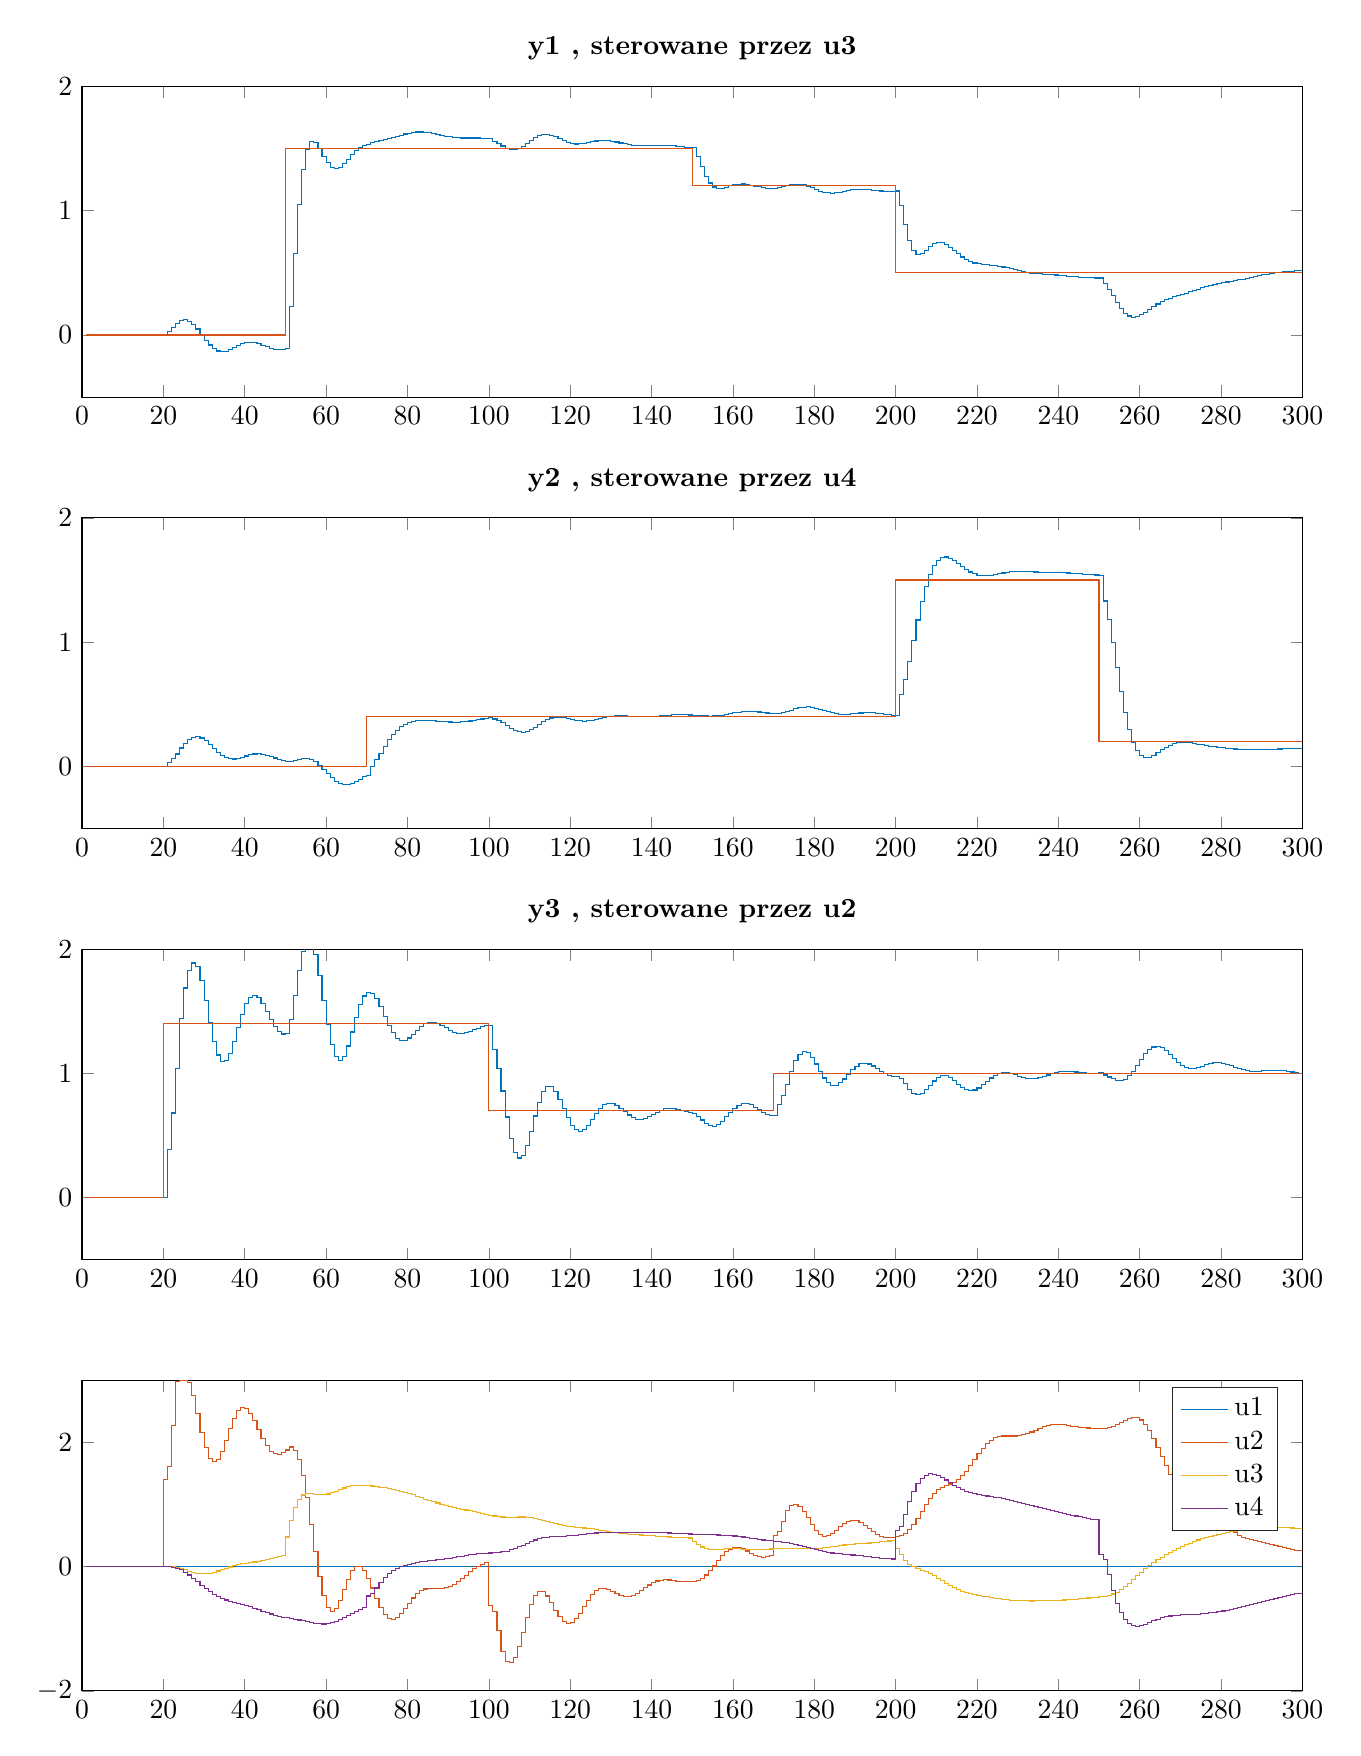
\begin{tikzpicture}

\begin{axis}[%
width=6.102in,
height=1.553in,
at={(1.024in,7.552in)},
scale only axis,
xmin=0,
xmax=300,
ymin=-0.5,
ymax=2,
axis background/.style={fill=white},
title style={font=\bfseries},
title={y1 , sterowane przez u3}
]
\addplot[const plot, color=mycolor1, forget plot] table[row sep=crcr] {%
1	0\\
2	0\\
3	0\\
4	0\\
5	0\\
6	0\\
7	0\\
8	0\\
9	0\\
10	0\\
11	0\\
12	0\\
13	0\\
14	0\\
15	0\\
16	0\\
17	0\\
18	0\\
19	0\\
20	0\\
21	0.0311227298218533\\
22	0.060006319733933\\
23	0.0892979253966268\\
24	0.116432884576393\\
25	0.123523949360394\\
26	0.111484355727959\\
27	0.0853495079407545\\
28	0.0479045611041573\\
29	0.00369814893013314\\
30	-0.0411107939506653\\
31	-0.0807802749199079\\
32	-0.110958018266106\\
33	-0.12911359082734\\
34	-0.134794797643479\\
35	-0.129523691811492\\
36	-0.116328262433713\\
37	-0.099067253800732\\
38	-0.0816968240069061\\
39	-0.0676049168705297\\
40	-0.0591189523850878\\
41	-0.0572518575786083\\
42	-0.0617009816484797\\
43	-0.0710690286227898\\
44	-0.083242322297704\\
45	-0.0958429135432966\\
46	-0.106668752198288\\
47	-0.114048815270845\\
48	-0.117063611625127\\
49	-0.115610484777499\\
50	-0.110322012863533\\
51	0.227913314142859\\
52	0.658844160869814\\
53	1.04827194036798\\
54	1.33203660909863\\
55	1.4964538370115\\
56	1.55824520927233\\
57	1.54805621026617\\
58	1.49864222218715\\
59	1.43775771695527\\
60	1.38500181867308\\
61	1.35140754677381\\
62	1.34062579392343\\
63	1.35084031966561\\
64	1.37683441736723\\
65	1.41186454566928\\
66	1.4491686865167\\
67	1.48304644897941\\
68	1.50951035963987\\
69	1.52654378865598\\
70	1.53402448082195\\
71	1.54677992241519\\
72	1.55467923054516\\
73	1.56173215478118\\
74	1.56990785077232\\
75	1.57898000050709\\
76	1.58863238849466\\
77	1.59855867447749\\
78	1.60829469533326\\
79	1.61725847753401\\
80	1.62482815956244\\
81	1.63041980642352\\
82	1.63357867384393\\
83	1.63406718919578\\
84	1.63192333863146\\
85	1.62747276014015\\
86	1.62129006544816\\
87	1.61411618296452\\
88	1.60674773531153\\
89	1.59991967647396\\
90	1.59420268105467\\
91	1.58993264051409\\
92	1.58718246319026\\
93	1.58577793560716\\
94	1.58535143129398\\
95	1.5854211882815\\
96	1.58548061605253\\
97	1.58508190847849\\
98	1.58390081551552\\
99	1.58177399553674\\
100	1.5787059070053\\
101	1.55928626791181\\
102	1.54045128041245\\
103	1.521182666807\\
104	1.50306259839512\\
105	1.49161549937417\\
106	1.49014055111981\\
107	1.4990152739091\\
108	1.51667074153156\\
109	1.53999899720784\\
110	1.56495643569632\\
111	1.58746207983769\\
112	1.60419051594983\\
113	1.61309140001022\\
114	1.61361532361248\\
115	1.6066478024918\\
116	1.59419522510879\\
117	1.57891157475882\\
118	1.56357101351455\\
119	1.55058470645712\\
120	1.54163933165601\\
121	1.53750390812446\\
122	1.53801670305634\\
123	1.54223171825803\\
124	1.54867975264875\\
125	1.55568531627032\\
126	1.56167862775835\\
127	1.56545042245881\\
128	1.56631356185813\\
129	1.56415573962705\\
130	1.55938799048066\\
131	1.55281076578095\\
132	1.54543058174891\\
133	1.53826449809378\\
134	1.53216709935316\\
135	1.52770651728351\\
136	1.52510441716327\\
137	1.52424217297401\\
138	1.52472396051974\\
139	1.52597900107204\\
140	1.52738075769827\\
141	1.52836076780976\\
142	1.52849847367921\\
143	1.52757479346846\\
144	1.52558484227186\\
145	1.52271270709731\\
146	1.51927725291606\\
147	1.51566173583265\\
148	1.51224116208511\\
149	1.50931998760548\\
150	1.50708944060014\\
151	1.43955267585967\\
152	1.35440510483044\\
153	1.27803344206715\\
154	1.22280712290674\\
155	1.19107004910472\\
156	1.17921207845537\\
157	1.18099424593786\\
158	1.18991035033558\\
159	1.20058180469411\\
160	1.20934298451155\\
161	1.21426959447624\\
162	1.21488998536984\\
163	1.21176072825628\\
164	1.20602804309649\\
165	1.19904629798219\\
166	1.19208688940175\\
167	1.18614616641243\\
168	1.18184679425884\\
169	1.17941915802889\\
170	1.17874525249988\\
171	1.18611460880873\\
172	1.19384651771007\\
173	1.20193743062117\\
174	1.20932787518186\\
175	1.21338133612726\\
176	1.21255479212841\\
177	1.20669779437632\\
178	1.19661220068342\\
179	1.18383904955503\\
180	1.17035361658419\\
181	1.1581348074796\\
182	1.14878778745328\\
183	1.1432970274082\\
184	1.14192076674973\\
185	1.14422561593082\\
186	1.1492395556526\\
187	1.15568066263872\\
188	1.16221123376094\\
189	1.16767014195462\\
190	1.17124632046204\\
191	1.17257109449136\\
192	1.17172382966458\\
193	1.16916085932217\\
194	1.16558941651163\\
195	1.16181487156533\\
196	1.15859053065847\\
197	1.15649513531186\\
198	1.15585535336453\\
199	1.15672076469113\\
200	1.15888901551203\\
201	1.04466025717873\\
202	0.890267737613763\\
203	0.760014988040286\\
204	0.680314664583476\\
205	0.649798518257329\\
206	0.65538658263557\\
207	0.680596775138919\\
208	0.710392015689639\\
209	0.733959686193351\\
210	0.745467885774434\\
211	0.743448566173728\\
212	0.729561884761566\\
213	0.707243015429482\\
214	0.680517314622223\\
215	0.653122402947276\\
216	0.627968321594498\\
217	0.606899892595478\\
218	0.590694433097569\\
219	0.579220339315834\\
220	0.571686908633089\\
221	0.566926536360737\\
222	0.563663389436175\\
223	0.560735948735955\\
224	0.557253648759987\\
225	0.552679821956514\\
226	0.546843803941178\\
227	0.53989375583296\\
228	0.532207866690728\\
229	0.524284639427371\\
230	0.516632808351637\\
231	0.509678387456142\\
232	0.503701116100706\\
233	0.498806152487748\\
234	0.494930374591669\\
235	0.49187710723441\\
236	0.489369274740239\\
237	0.487109292107607\\
238	0.484834469486509\\
239	0.482358973449664\\
240	0.479596862134684\\
241	0.476564658517195\\
242	0.473365624802651\\
243	0.470160759351403\\
244	0.46713317848338\\
245	0.464452844155983\\
246	0.462247672713545\\
247	0.460585220304969\\
248	0.459466814103278\\
249	0.45883364157279\\
250	0.458582327539908\\
251	0.415069644006618\\
252	0.36920183268233\\
253	0.317509578907267\\
254	0.262938437061066\\
255	0.213861593910531\\
256	0.176234735237136\\
257	0.152846543362673\\
258	0.144005828798657\\
259	0.148024467795527\\
260	0.161888285378149\\
261	0.182048726897611\\
262	0.205103895402879\\
263	0.228269693625968\\
264	0.249628175864193\\
265	0.268174116927345\\
266	0.283704041848828\\
267	0.2966057706412\\
268	0.307607438154258\\
269	0.317536441493157\\
270	0.327125155953609\\
271	0.336884512002269\\
272	0.347051084224025\\
273	0.357600270794512\\
274	0.368308832414248\\
275	0.378845153903697\\
276	0.388865034842566\\
277	0.39809395453493\\
278	0.406382496029986\\
279	0.413728627329219\\
280	0.420267493516501\\
281	0.426235138172995\\
282	0.43191636318782\\
283	0.437588400402822\\
284	0.443471286132046\\
285	0.44969324380484\\
286	0.456275677701323\\
287	0.463138346721893\\
288	0.47012165984095\\
289	0.477020388071344\\
290	0.483621754352211\\
291	0.489740908979515\\
292	0.495248045903519\\
293	0.50008350295564\\
294	0.504259656512466\\
295	0.507850799810375\\
296	0.510974088351353\\
297	0.51376578098545\\
298	0.516357296731986\\
299	0.518855098739406\\
300	0.521327291076846\\
};
\addplot[const plot, color=mycolor2, forget plot] table[row sep=crcr] {%
1	0\\
2	0\\
3	0\\
4	0\\
5	0\\
6	0\\
7	0\\
8	0\\
9	0\\
10	0\\
11	0\\
12	0\\
13	0\\
14	0\\
15	0\\
16	0\\
17	0\\
18	0\\
19	0\\
20	0\\
21	0\\
22	0\\
23	0\\
24	0\\
25	0\\
26	0\\
27	0\\
28	0\\
29	0\\
30	0\\
31	0\\
32	0\\
33	0\\
34	0\\
35	0\\
36	0\\
37	0\\
38	0\\
39	0\\
40	0\\
41	0\\
42	0\\
43	0\\
44	0\\
45	0\\
46	0\\
47	0\\
48	0\\
49	0\\
50	1.5\\
51	1.5\\
52	1.5\\
53	1.5\\
54	1.5\\
55	1.5\\
56	1.5\\
57	1.5\\
58	1.5\\
59	1.5\\
60	1.5\\
61	1.5\\
62	1.5\\
63	1.5\\
64	1.5\\
65	1.5\\
66	1.5\\
67	1.5\\
68	1.5\\
69	1.5\\
70	1.5\\
71	1.5\\
72	1.5\\
73	1.5\\
74	1.5\\
75	1.5\\
76	1.5\\
77	1.5\\
78	1.5\\
79	1.5\\
80	1.5\\
81	1.5\\
82	1.5\\
83	1.5\\
84	1.5\\
85	1.5\\
86	1.5\\
87	1.5\\
88	1.5\\
89	1.5\\
90	1.5\\
91	1.5\\
92	1.5\\
93	1.5\\
94	1.5\\
95	1.5\\
96	1.5\\
97	1.5\\
98	1.5\\
99	1.5\\
100	1.5\\
101	1.5\\
102	1.5\\
103	1.5\\
104	1.5\\
105	1.5\\
106	1.5\\
107	1.5\\
108	1.5\\
109	1.5\\
110	1.5\\
111	1.5\\
112	1.5\\
113	1.5\\
114	1.5\\
115	1.5\\
116	1.5\\
117	1.5\\
118	1.5\\
119	1.5\\
120	1.5\\
121	1.5\\
122	1.5\\
123	1.5\\
124	1.5\\
125	1.5\\
126	1.5\\
127	1.5\\
128	1.5\\
129	1.5\\
130	1.5\\
131	1.5\\
132	1.5\\
133	1.5\\
134	1.5\\
135	1.5\\
136	1.5\\
137	1.5\\
138	1.5\\
139	1.5\\
140	1.5\\
141	1.5\\
142	1.5\\
143	1.5\\
144	1.5\\
145	1.5\\
146	1.5\\
147	1.5\\
148	1.5\\
149	1.5\\
150	1.2\\
151	1.2\\
152	1.2\\
153	1.2\\
154	1.2\\
155	1.2\\
156	1.2\\
157	1.2\\
158	1.2\\
159	1.2\\
160	1.2\\
161	1.2\\
162	1.2\\
163	1.2\\
164	1.2\\
165	1.2\\
166	1.2\\
167	1.2\\
168	1.2\\
169	1.2\\
170	1.2\\
171	1.2\\
172	1.2\\
173	1.2\\
174	1.2\\
175	1.2\\
176	1.2\\
177	1.2\\
178	1.2\\
179	1.2\\
180	1.2\\
181	1.2\\
182	1.2\\
183	1.2\\
184	1.2\\
185	1.2\\
186	1.2\\
187	1.2\\
188	1.2\\
189	1.2\\
190	1.2\\
191	1.2\\
192	1.2\\
193	1.2\\
194	1.2\\
195	1.2\\
196	1.2\\
197	1.2\\
198	1.2\\
199	1.2\\
200	0.5\\
201	0.5\\
202	0.5\\
203	0.5\\
204	0.5\\
205	0.5\\
206	0.5\\
207	0.5\\
208	0.5\\
209	0.5\\
210	0.5\\
211	0.5\\
212	0.5\\
213	0.5\\
214	0.5\\
215	0.5\\
216	0.5\\
217	0.5\\
218	0.5\\
219	0.5\\
220	0.5\\
221	0.5\\
222	0.5\\
223	0.5\\
224	0.5\\
225	0.5\\
226	0.5\\
227	0.5\\
228	0.5\\
229	0.5\\
230	0.5\\
231	0.5\\
232	0.5\\
233	0.5\\
234	0.5\\
235	0.5\\
236	0.5\\
237	0.5\\
238	0.5\\
239	0.5\\
240	0.5\\
241	0.5\\
242	0.5\\
243	0.5\\
244	0.5\\
245	0.5\\
246	0.5\\
247	0.5\\
248	0.5\\
249	0.5\\
250	0.5\\
251	0.5\\
252	0.5\\
253	0.5\\
254	0.5\\
255	0.5\\
256	0.5\\
257	0.5\\
258	0.5\\
259	0.5\\
260	0.5\\
261	0.5\\
262	0.5\\
263	0.5\\
264	0.5\\
265	0.5\\
266	0.5\\
267	0.5\\
268	0.5\\
269	0.5\\
270	0.5\\
271	0.5\\
272	0.5\\
273	0.5\\
274	0.5\\
275	0.5\\
276	0.5\\
277	0.5\\
278	0.5\\
279	0.5\\
280	0.5\\
281	0.5\\
282	0.5\\
283	0.5\\
284	0.5\\
285	0.5\\
286	0.5\\
287	0.5\\
288	0.5\\
289	0.5\\
290	0.5\\
291	0.5\\
292	0.5\\
293	0.5\\
294	0.5\\
295	0.5\\
296	0.5\\
297	0.5\\
298	0.5\\
299	0.5\\
300	0.5\\
};
\end{axis}

\begin{axis}[%
width=6.102in,
height=1.553in,
at={(1.024in,5.395in)},
scale only axis,
xmin=0,
xmax=300,
ymin=-0.5,
ymax=2,
axis background/.style={fill=white},
title style={font=\bfseries},
title={y2 , sterowane przez u4}
]
\addplot[const plot, color=mycolor1, forget plot] table[row sep=crcr] {%
1	0\\
2	0\\
3	0\\
4	0\\
5	0\\
6	0\\
7	0\\
8	0\\
9	0\\
10	0\\
11	0\\
12	0\\
13	0\\
14	0\\
15	0\\
16	0\\
17	0\\
18	0\\
19	0\\
20	0\\
21	0.0287102169237213\\
22	0.0605338613118116\\
23	0.0998675547359671\\
24	0.147651754824526\\
25	0.187139865474448\\
26	0.215833382798195\\
27	0.233850191709184\\
28	0.238223252974824\\
29	0.228470933209169\\
30	0.207183765791091\\
31	0.178210753175674\\
32	0.145956482436877\\
33	0.114890817670103\\
34	0.0888216783667646\\
35	0.0703247242137098\\
36	0.0604864226769908\\
37	0.0589143053726732\\
38	0.0639750353367584\\
39	0.0732075337292581\\
40	0.0838235802457153\\
41	0.0932007573746083\\
42	0.0992873549509969\\
43	0.100863304006914\\
44	0.097631407405748\\
45	0.0901445587054113\\
46	0.0796014385580409\\
47	0.0675611729834019\\
48	0.0556347518713987\\
49	0.0452077330020637\\
50	0.0372367201438612\\
51	0.0373783455544194\\
52	0.0445462106846827\\
53	0.0539214927255068\\
54	0.0610920027028724\\
55	0.0622142160564423\\
56	0.0543948271431684\\
57	0.0365681444941507\\
58	0.00974700302526334\\
59	-0.0233070767084022\\
60	-0.0586858067447401\\
61	-0.092088542950623\\
62	-0.119604831005618\\
63	-0.13836885539985\\
64	-0.146973346035142\\
65	-0.145594437200693\\
66	-0.135834804809571\\
67	-0.120340113922751\\
68	-0.102277891817875\\
69	-0.0847822597310066\\
70	-0.0704622883884091\\
71	0.00249541244182128\\
72	0.0523325777126791\\
73	0.105912458643455\\
74	0.162346530173795\\
75	0.213368489122693\\
76	0.256259282053268\\
77	0.290771986697449\\
78	0.317339983846244\\
79	0.336921206996125\\
80	0.350744978227932\\
81	0.360015418082227\\
82	0.365757385067377\\
83	0.368778111447447\\
84	0.36969530022506\\
85	0.369000107221025\\
86	0.367127133998837\\
87	0.36450856772644\\
88	0.361599364114764\\
89	0.358870717298255\\
90	0.356777506074444\\
91	0.355710971733392\\
92	0.355950132567376\\
93	0.357624490285727\\
94	0.360697118602251\\
95	0.364972289585196\\
96	0.37012654068095\\
97	0.37575755686763\\
98	0.381442206611606\\
99	0.386793923914684\\
100	0.391510376108139\\
101	0.381049552392895\\
102	0.368149629668039\\
103	0.350670185288915\\
104	0.328291905841882\\
105	0.306214217959423\\
106	0.288617417140707\\
107	0.277975811741427\\
108	0.275851061425344\\
109	0.282502756945479\\
110	0.29670742405077\\
111	0.316129329180396\\
112	0.337835053042679\\
113	0.358811811569237\\
114	0.376458524257974\\
115	0.388968015601588\\
116	0.395534853107053\\
117	0.396373440524028\\
118	0.392566250635727\\
119	0.385786258410239\\
120	0.377954013940544\\
121	0.370894340301614\\
122	0.36605005631529\\
123	0.364293671728528\\
124	0.365856678075323\\
125	0.370373962394365\\
126	0.377021831721041\\
127	0.384715032201909\\
128	0.392322475622863\\
129	0.398863197943321\\
130	0.4036521493622\\
131	0.406377622714677\\
132	0.407105896623981\\
133	0.406221483114758\\
134	0.404321179489273\\
135	0.4020856445587\\
136	0.400153047581415\\
137	0.399015915686189\\
138	0.39895573793846\\
139	0.400021672591118\\
140	0.402051441767128\\
141	0.404725589280877\\
142	0.407641723666267\\
143	0.410393648041551\\
144	0.412641330442719\\
145	0.414160969974181\\
146	0.414869126664009\\
147	0.414820032497469\\
148	0.414179860759419\\
149	0.413185171597032\\
150	0.412094541650118\\
151	0.41009563766073\\
152	0.407557214748807\\
153	0.405423257394681\\
154	0.404410822767023\\
155	0.405024668068056\\
156	0.407538722777144\\
157	0.411878020430307\\
158	0.417615881832275\\
159	0.424070436398275\\
160	0.430435668976579\\
161	0.435923749769868\\
162	0.439897621676099\\
163	0.441968570555842\\
164	0.44204311124098\\
165	0.440315898708296\\
166	0.437215093423327\\
167	0.433314042798961\\
168	0.429227626757301\\
169	0.425512348564928\\
170	0.42258652453476\\
171	0.426833890312339\\
172	0.432801444037218\\
173	0.441284943269572\\
174	0.452208708099428\\
175	0.463088555882392\\
176	0.471882833976972\\
177	0.477328863013897\\
178	0.478631753986812\\
179	0.475643626776029\\
180	0.46893695831618\\
181	0.459627652362272\\
182	0.44912744938191\\
183	0.438891376094367\\
184	0.430179075255093\\
185	0.423869488832315\\
186	0.420359770784209\\
187	0.419555872375848\\
188	0.420945271699845\\
189	0.423730500737621\\
190	0.42699424447024\\
191	0.429864648112014\\
192	0.431653147525252\\
193	0.431945086497511\\
194	0.430633680243361\\
195	0.427898542084023\\
196	0.424139163811427\\
197	0.419880045988034\\
198	0.41566689377321\\
199	0.411972406179701\\
200	0.409126283125548\\
201	0.5795852490889\\
202	0.700822018080533\\
203	0.847581942578567\\
204	1.01556149823209\\
205	1.1783380281721\\
206	1.32384917014026\\
207	1.44657520053726\\
208	1.54331076044889\\
209	1.61336725502366\\
210	1.65825738547953\\
211	1.68098496769648\\
212	1.68547830226863\\
213	1.67613873884581\\
214	1.65744425709318\\
215	1.63361295064064\\
216	1.6083365620828\\
217	1.58458906158355\\
218	1.56451481311036\\
219	1.54939836658939\\
220	1.53971207661952\\
221	1.5352307361563\\
222	1.53519597318984\\
223	1.53850853287399\\
224	1.54392469503355\\
225	1.55023437135016\\
226	1.55640267012799\\
227	1.56166316011073\\
228	1.56555861659617\\
229	1.56793247948397\\
230	1.56888048045063\\
231	1.56867607638784\\
232	1.56768503037527\\
233	1.56628371668481\\
234	1.56479289107558\\
235	1.56343444641567\\
236	1.56231389438591\\
237	1.56142679689097\\
238	1.56068379520405\\
239	1.55994669477294\\
240	1.55906742301069\\
241	1.5579224774435\\
242	1.55643739217685\\
243	1.55459830244459\\
244	1.55245036665095\\
245	1.55008514612833\\
246	1.5476206965019\\
247	1.54517890405807\\
248	1.54286449066909\\
249	1.54074924868063\\
250	1.53886369932017\\
251	1.33067457508891\\
252	1.1796217945737\\
253	0.999432194834302\\
254	0.796740063213172\\
255	0.603905793778009\\
256	0.435875368844386\\
257	0.299080786075957\\
258	0.196387255790523\\
259	0.127059758827436\\
260	0.0874310233038617\\
261	0.0720732313108107\\
262	0.0747887769659666\\
263	0.0893895201289868\\
264	0.110293790489271\\
265	0.1329236470987\\
266	0.153902438710149\\
267	0.171077597057021\\
268	0.183406256486027\\
269	0.190747360120745\\
270	0.193605349583979\\
271	0.192866978787805\\
272	0.189564985937153\\
273	0.184691875651822\\
274	0.179075602125931\\
275	0.173318091712424\\
276	0.167788627731946\\
277	0.162658043428344\\
278	0.157956810526576\\
279	0.153640334550873\\
280	0.149647507356637\\
281	0.14594296565654\\
282	0.142538584086366\\
283	0.139494561606568\\
284	0.136904295629954\\
285	0.134869611492829\\
286	0.133473670615168\\
287	0.132758156390511\\
288	0.132709497679441\\
289	0.133256435223033\\
290	0.134278697263471\\
291	0.135624395466668\\
292	0.137132315792268\\
293	0.138654723989318\\
294	0.140076618038527\\
295	0.141328375754673\\
296	0.142390198352719\\
297	0.143288330730152\\
298	0.144084453406746\\
299	0.144860661218985\\
300	0.145702937868377\\
};
\addplot[const plot, color=mycolor2, forget plot] table[row sep=crcr] {%
1	0\\
2	0\\
3	0\\
4	0\\
5	0\\
6	0\\
7	0\\
8	0\\
9	0\\
10	0\\
11	0\\
12	0\\
13	0\\
14	0\\
15	0\\
16	0\\
17	0\\
18	0\\
19	0\\
20	0\\
21	0\\
22	0\\
23	0\\
24	0\\
25	0\\
26	0\\
27	0\\
28	0\\
29	0\\
30	0\\
31	0\\
32	0\\
33	0\\
34	0\\
35	0\\
36	0\\
37	0\\
38	0\\
39	0\\
40	0\\
41	0\\
42	0\\
43	0\\
44	0\\
45	0\\
46	0\\
47	0\\
48	0\\
49	0\\
50	0\\
51	0\\
52	0\\
53	0\\
54	0\\
55	0\\
56	0\\
57	0\\
58	0\\
59	0\\
60	0\\
61	0\\
62	0\\
63	0\\
64	0\\
65	0\\
66	0\\
67	0\\
68	0\\
69	0\\
70	0.4\\
71	0.4\\
72	0.4\\
73	0.4\\
74	0.4\\
75	0.4\\
76	0.4\\
77	0.4\\
78	0.4\\
79	0.4\\
80	0.4\\
81	0.4\\
82	0.4\\
83	0.4\\
84	0.4\\
85	0.4\\
86	0.4\\
87	0.4\\
88	0.4\\
89	0.4\\
90	0.4\\
91	0.4\\
92	0.4\\
93	0.4\\
94	0.4\\
95	0.4\\
96	0.4\\
97	0.4\\
98	0.4\\
99	0.4\\
100	0.4\\
101	0.4\\
102	0.4\\
103	0.4\\
104	0.4\\
105	0.4\\
106	0.4\\
107	0.4\\
108	0.4\\
109	0.4\\
110	0.4\\
111	0.4\\
112	0.4\\
113	0.4\\
114	0.4\\
115	0.4\\
116	0.4\\
117	0.4\\
118	0.4\\
119	0.4\\
120	0.4\\
121	0.4\\
122	0.4\\
123	0.4\\
124	0.4\\
125	0.4\\
126	0.4\\
127	0.4\\
128	0.4\\
129	0.4\\
130	0.4\\
131	0.4\\
132	0.4\\
133	0.4\\
134	0.4\\
135	0.4\\
136	0.4\\
137	0.4\\
138	0.4\\
139	0.4\\
140	0.4\\
141	0.4\\
142	0.4\\
143	0.4\\
144	0.4\\
145	0.4\\
146	0.4\\
147	0.4\\
148	0.4\\
149	0.4\\
150	0.4\\
151	0.4\\
152	0.4\\
153	0.4\\
154	0.4\\
155	0.4\\
156	0.4\\
157	0.4\\
158	0.4\\
159	0.4\\
160	0.4\\
161	0.4\\
162	0.4\\
163	0.4\\
164	0.4\\
165	0.4\\
166	0.4\\
167	0.4\\
168	0.4\\
169	0.4\\
170	0.4\\
171	0.4\\
172	0.4\\
173	0.4\\
174	0.4\\
175	0.4\\
176	0.4\\
177	0.4\\
178	0.4\\
179	0.4\\
180	0.4\\
181	0.4\\
182	0.4\\
183	0.4\\
184	0.4\\
185	0.4\\
186	0.4\\
187	0.4\\
188	0.4\\
189	0.4\\
190	0.4\\
191	0.4\\
192	0.4\\
193	0.4\\
194	0.4\\
195	0.4\\
196	0.4\\
197	0.4\\
198	0.4\\
199	0.4\\
200	1.5\\
201	1.5\\
202	1.5\\
203	1.5\\
204	1.5\\
205	1.5\\
206	1.5\\
207	1.5\\
208	1.5\\
209	1.5\\
210	1.5\\
211	1.5\\
212	1.5\\
213	1.5\\
214	1.5\\
215	1.5\\
216	1.5\\
217	1.5\\
218	1.5\\
219	1.5\\
220	1.5\\
221	1.5\\
222	1.5\\
223	1.5\\
224	1.5\\
225	1.5\\
226	1.5\\
227	1.5\\
228	1.5\\
229	1.5\\
230	1.5\\
231	1.5\\
232	1.5\\
233	1.5\\
234	1.5\\
235	1.5\\
236	1.5\\
237	1.5\\
238	1.5\\
239	1.5\\
240	1.5\\
241	1.5\\
242	1.5\\
243	1.5\\
244	1.5\\
245	1.5\\
246	1.5\\
247	1.5\\
248	1.5\\
249	1.5\\
250	0.2\\
251	0.2\\
252	0.2\\
253	0.2\\
254	0.2\\
255	0.2\\
256	0.2\\
257	0.2\\
258	0.2\\
259	0.2\\
260	0.2\\
261	0.2\\
262	0.2\\
263	0.2\\
264	0.2\\
265	0.2\\
266	0.2\\
267	0.2\\
268	0.2\\
269	0.2\\
270	0.2\\
271	0.2\\
272	0.2\\
273	0.2\\
274	0.2\\
275	0.2\\
276	0.2\\
277	0.2\\
278	0.2\\
279	0.2\\
280	0.2\\
281	0.2\\
282	0.2\\
283	0.2\\
284	0.2\\
285	0.2\\
286	0.2\\
287	0.2\\
288	0.2\\
289	0.2\\
290	0.2\\
291	0.2\\
292	0.2\\
293	0.2\\
294	0.2\\
295	0.2\\
296	0.2\\
297	0.2\\
298	0.2\\
299	0.2\\
300	0.2\\
};
\end{axis}

\begin{axis}[%
width=6.102in,
height=1.553in,
at={(1.024in,3.239in)},
scale only axis,
xmin=0,
xmax=300,
ymin=-0.5,
ymax=2,
axis background/.style={fill=white},
title style={font=\bfseries},
title={y3 , sterowane przez u2}
]
\addplot[const plot, color=mycolor1, forget plot] table[row sep=crcr] {%
1	0\\
2	0\\
3	0\\
4	0\\
5	0\\
6	0\\
7	0\\
8	0\\
9	0\\
10	0\\
11	0\\
12	0\\
13	0\\
14	0\\
15	0\\
16	0\\
17	0\\
18	0\\
19	0\\
20	0\\
21	0.387527953249027\\
22	0.680415531412489\\
23	1.03762936317039\\
24	1.44191633259115\\
25	1.68683551348615\\
26	1.82538712555885\\
27	1.8881695856669\\
28	1.85704991729333\\
29	1.74438744930146\\
30	1.58452009420064\\
31	1.41213540755651\\
32	1.25815789209397\\
33	1.14726854705877\\
34	1.093915867963\\
35	1.10075696095327\\
36	1.15981751860544\\
37	1.25521953222878\\
38	1.36682100542875\\
39	1.47415518998062\\
40	1.55995242135208\\
41	1.61267794498326\\
42	1.62778151970151\\
43	1.60760974865174\\
44	1.56016011090226\\
45	1.49703055245103\\
46	1.43101195040115\\
47	1.37377577594702\\
48	1.33403706186697\\
49	1.31644525326683\\
50	1.32130092562782\\
51	1.43628892444388\\
52	1.62659277320081\\
53	1.82519719260521\\
54	1.98304780341607\\
55	2.06536008066503\\
56	2.05442389349029\\
57	1.95441945052201\\
58	1.78810135976593\\
59	1.58916804556566\\
60	1.3942299907871\\
61	1.23554410132362\\
62	1.13548771845733\\
63	1.10362205923956\\
64	1.13651596656573\\
65	1.21992705842682\\
66	1.33261277958097\\
67	1.45088202805365\\
68	1.5529944988386\\
69	1.62266501625819\\
70	1.65118596213235\\
71	1.64450667647236\\
72	1.60251883048898\\
73	1.53651918741682\\
74	1.46067191247722\\
75	1.38695941410796\\
76	1.3255152781928\\
77	1.28349402004889\\
78	1.26389775046329\\
79	1.2656931076366\\
80	1.28463577113579\\
81	1.31439486992268\\
82	1.34785938867572\\
83	1.37841605966839\\
84	1.40097133539924\\
85	1.41258083350373\\
86	1.41263837283252\\
87	1.40265073140731\\
88	1.38568871787841\\
89	1.36564847452359\\
90	1.3464716371881\\
91	1.33146075447819\\
92	1.32279302647618\\
93	1.32128898416039\\
94	1.32644255057301\\
95	1.33667395672043\\
96	1.34973417133541\\
97	1.36317285997682\\
98	1.37478221116522\\
99	1.38294408756405\\
100	1.3868334755509\\
101	1.19269752487569\\
102	1.04236286563302\\
103	0.857603535425144\\
104	0.648540864441251\\
105	0.474195026310077\\
106	0.361847772091623\\
107	0.318070965235482\\
108	0.341289078993348\\
109	0.419706342144554\\
110	0.532790100136065\\
111	0.656637589520125\\
112	0.768692625621331\\
113	0.851219405498445\\
114	0.89368220179608\\
115	0.893678257616933\\
116	0.856340880706861\\
117	0.792528818233121\\
118	0.716275737875537\\
119	0.642017186552021\\
120	0.582090423596278\\
121	0.544899051856711\\
122	0.533971918317704\\
123	0.547965025111291\\
124	0.581489508922517\\
125	0.626523211380594\\
126	0.674094334690179\\
127	0.715918073619071\\
128	0.745714586213192\\
129	0.760024301734057\\
130	0.758444541529937\\
131	0.743318928480904\\
132	0.718999917011146\\
133	0.690862234665252\\
134	0.664265237460368\\
135	0.643646331747678\\
136	0.631882856805121\\
137	0.629997320403764\\
138	0.637213423997651\\
139	0.651309950312052\\
140	0.669175665643529\\
141	0.687446319002678\\
142	0.7031056346533\\
143	0.713952921684687\\
144	0.718874585608599\\
145	0.717897823245084\\
146	0.712044381606641\\
147	0.703033926616241\\
148	0.692905915016703\\
149	0.683634139672644\\
150	0.676800173095287\\
151	0.655124815056239\\
152	0.624572899128331\\
153	0.596617555071439\\
154	0.578650681697948\\
155	0.575191681338265\\
156	0.587741974544203\\
157	0.614118557212134\\
158	0.649259666988163\\
159	0.686734068166466\\
160	0.720193839908826\\
161	0.744580161045473\\
162	0.756940911420707\\
163	0.756743851599463\\
164	0.745695988369629\\
165	0.727179075258523\\
166	0.705457630652994\\
167	0.684830183332999\\
168	0.668880568998735\\
169	0.659946975954535\\
170	0.658872525763388\\
171	0.748085917757098\\
172	0.822480110856099\\
173	0.913611053071907\\
174	1.01506713853857\\
175	1.099742014269\\
176	1.1546695998225\\
177	1.17644788512387\\
178	1.16586959601137\\
179	1.1287038784323\\
180	1.07486583713352\\
181	1.01587771316193\\
182	0.962610623217236\\
183	0.923600853417542\\
184	0.903904813121915\\
185	0.904656379130982\\
186	0.923359260598574\\
187	0.95476288644541\\
188	0.99209396180775\\
189	1.02839371282847\\
190	1.05772200878868\\
191	1.07603992143172\\
192	1.08166065120818\\
193	1.07524585676833\\
194	1.05940423737182\\
195	1.03800959340605\\
196	1.01538867907467\\
197	0.995532642026794\\
198	0.98146280805306\\
199	0.974839221874242\\
200	0.975848264617282\\
201	0.958715468471241\\
202	0.916042661635764\\
203	0.871405035771075\\
204	0.840972341891726\\
205	0.829972815051607\\
206	0.839563542169184\\
207	0.866311137403369\\
208	0.902402488316244\\
209	0.938516519662266\\
210	0.966460173354059\\
211	0.980770050660569\\
212	0.979515256432773\\
213	0.964296722030972\\
214	0.939506249849944\\
215	0.911118530547543\\
216	0.88533746306939\\
217	0.867373618820284\\
218	0.860560765057926\\
219	0.865928912546341\\
220	0.882251392265571\\
221	0.906495653695912\\
222	0.934545670865771\\
223	0.962033802042264\\
224	0.985122017282114\\
225	1.00110185891583\\
226	1.00873057905841\\
227	1.00827690386116\\
228	1.0013032409003\\
229	0.990253145238966\\
230	0.977937804414794\\
231	0.967021115451115\\
232	0.959591031154072\\
233	0.956879489386266\\
234	0.959160397227919\\
235	0.965821330086571\\
236	0.975575685708675\\
237	0.986762308775572\\
238	0.997671284557175\\
239	1.00683769340113\\
240	1.01325769027032\\
241	1.01650002563911\\
242	1.01670711660748\\
243	1.01449917776568\\
244	1.01080964088805\\
245	1.00668821638777\\
246	1.00310891694649\\
247	1.00081489568076\\
248	1.00022176939833\\
249	1.00138850917372\\
250	1.0040524150452\\
251	0.986509562258604\\
252	0.970104244048428\\
253	0.95600451254555\\
254	0.944404988929187\\
255	0.942033849400506\\
256	0.953369280824879\\
257	0.978971443133885\\
258	1.01692757692816\\
259	1.06310879451741\\
260	1.11165060309069\\
261	1.15613262301496\\
262	1.19081304590959\\
263	1.21159252841985\\
264	1.21662401792138\\
265	1.2064929630604\\
266	1.18395745192382\\
267	1.15333502983898\\
268	1.11968023186249\\
269	1.08791547386283\\
270	1.0620685038346\\
271	1.04473513631982\\
272	1.03683410802365\\
273	1.03766334117436\\
274	1.04521457527952\\
275	1.05666448899361\\
276	1.06894009664743\\
277	1.07925564970951\\
278	1.08553521691562\\
279	1.08666455854097\\
280	1.08255133973785\\
281	1.07400741363469\\
282	1.06249506400206\\
283	1.04979676146222\\
284	1.03767345312951\\
285	1.02757024465533\\
286	1.02041301517222\\
287	1.01651874466029\\
288	1.01562030797992\\
289	1.0169870769565\\
290	1.01960882764634\\
291	1.02240382315715\\
292	1.02441275721088\\
293	1.02494743751421\\
294	1.02367465089402\\
295	1.02062908401791\\
296	1.01616196822327\\
297	1.01084218734007\\
298	1.00533256664464\\
299	1.00026544498472\\
300	0.996138757392236\\
};
\addplot[const plot, color=mycolor2, forget plot] table[row sep=crcr] {%
1	0\\
2	0\\
3	0\\
4	0\\
5	0\\
6	0\\
7	0\\
8	0\\
9	0\\
10	0\\
11	0\\
12	0\\
13	0\\
14	0\\
15	0\\
16	0\\
17	0\\
18	0\\
19	0\\
20	1.4\\
21	1.4\\
22	1.4\\
23	1.4\\
24	1.4\\
25	1.4\\
26	1.4\\
27	1.4\\
28	1.4\\
29	1.4\\
30	1.4\\
31	1.4\\
32	1.4\\
33	1.4\\
34	1.4\\
35	1.4\\
36	1.4\\
37	1.4\\
38	1.4\\
39	1.4\\
40	1.4\\
41	1.4\\
42	1.4\\
43	1.4\\
44	1.4\\
45	1.4\\
46	1.4\\
47	1.4\\
48	1.4\\
49	1.4\\
50	1.4\\
51	1.4\\
52	1.4\\
53	1.4\\
54	1.4\\
55	1.4\\
56	1.4\\
57	1.4\\
58	1.4\\
59	1.4\\
60	1.4\\
61	1.4\\
62	1.4\\
63	1.4\\
64	1.4\\
65	1.4\\
66	1.4\\
67	1.4\\
68	1.4\\
69	1.4\\
70	1.4\\
71	1.4\\
72	1.4\\
73	1.4\\
74	1.4\\
75	1.4\\
76	1.4\\
77	1.4\\
78	1.4\\
79	1.4\\
80	1.4\\
81	1.4\\
82	1.4\\
83	1.4\\
84	1.4\\
85	1.4\\
86	1.4\\
87	1.4\\
88	1.4\\
89	1.4\\
90	1.4\\
91	1.4\\
92	1.4\\
93	1.4\\
94	1.4\\
95	1.4\\
96	1.4\\
97	1.4\\
98	1.4\\
99	1.4\\
100	0.7\\
101	0.7\\
102	0.7\\
103	0.7\\
104	0.7\\
105	0.7\\
106	0.7\\
107	0.7\\
108	0.7\\
109	0.7\\
110	0.7\\
111	0.7\\
112	0.7\\
113	0.7\\
114	0.7\\
115	0.7\\
116	0.7\\
117	0.7\\
118	0.7\\
119	0.7\\
120	0.7\\
121	0.7\\
122	0.7\\
123	0.7\\
124	0.7\\
125	0.7\\
126	0.7\\
127	0.7\\
128	0.7\\
129	0.7\\
130	0.7\\
131	0.7\\
132	0.7\\
133	0.7\\
134	0.7\\
135	0.7\\
136	0.7\\
137	0.7\\
138	0.7\\
139	0.7\\
140	0.7\\
141	0.7\\
142	0.7\\
143	0.7\\
144	0.7\\
145	0.7\\
146	0.7\\
147	0.7\\
148	0.7\\
149	0.7\\
150	0.7\\
151	0.7\\
152	0.7\\
153	0.7\\
154	0.7\\
155	0.7\\
156	0.7\\
157	0.7\\
158	0.7\\
159	0.7\\
160	0.7\\
161	0.7\\
162	0.7\\
163	0.7\\
164	0.7\\
165	0.7\\
166	0.7\\
167	0.7\\
168	0.7\\
169	0.7\\
170	1\\
171	1\\
172	1\\
173	1\\
174	1\\
175	1\\
176	1\\
177	1\\
178	1\\
179	1\\
180	1\\
181	1\\
182	1\\
183	1\\
184	1\\
185	1\\
186	1\\
187	1\\
188	1\\
189	1\\
190	1\\
191	1\\
192	1\\
193	1\\
194	1\\
195	1\\
196	1\\
197	1\\
198	1\\
199	1\\
200	1\\
201	1\\
202	1\\
203	1\\
204	1\\
205	1\\
206	1\\
207	1\\
208	1\\
209	1\\
210	1\\
211	1\\
212	1\\
213	1\\
214	1\\
215	1\\
216	1\\
217	1\\
218	1\\
219	1\\
220	1\\
221	1\\
222	1\\
223	1\\
224	1\\
225	1\\
226	1\\
227	1\\
228	1\\
229	1\\
230	1\\
231	1\\
232	1\\
233	1\\
234	1\\
235	1\\
236	1\\
237	1\\
238	1\\
239	1\\
240	1\\
241	1\\
242	1\\
243	1\\
244	1\\
245	1\\
246	1\\
247	1\\
248	1\\
249	1\\
250	1\\
251	1\\
252	1\\
253	1\\
254	1\\
255	1\\
256	1\\
257	1\\
258	1\\
259	1\\
260	1\\
261	1\\
262	1\\
263	1\\
264	1\\
265	1\\
266	1\\
267	1\\
268	1\\
269	1\\
270	1\\
271	1\\
272	1\\
273	1\\
274	1\\
275	1\\
276	1\\
277	1\\
278	1\\
279	1\\
280	1\\
281	1\\
282	1\\
283	1\\
284	1\\
285	1\\
286	1\\
287	1\\
288	1\\
289	1\\
290	1\\
291	1\\
292	1\\
293	1\\
294	1\\
295	1\\
296	1\\
297	1\\
298	1\\
299	1\\
300	1\\
};
\end{axis}

\begin{axis}[%
width=6.102in,
height=1.553in,
at={(1.024in,1.083in)},
scale only axis,
xmin=0,
xmax=300,
ymin=-2,
ymax=3,
axis background/.style={fill=white},
legend style={legend cell align=left, align=left, draw=white!15!black}
]
\addplot[const plot, color=mycolor1] table[row sep=crcr] {%
1	0\\
2	0\\
3	0\\
4	0\\
5	0\\
6	0\\
7	0\\
8	0\\
9	0\\
10	0\\
11	0\\
12	0\\
13	0\\
14	0\\
15	0\\
16	0\\
17	0\\
18	0\\
19	0\\
20	0\\
21	0\\
22	0\\
23	0\\
24	0\\
25	0\\
26	0\\
27	0\\
28	0\\
29	0\\
30	0\\
31	0\\
32	0\\
33	0\\
34	0\\
35	0\\
36	0\\
37	0\\
38	0\\
39	0\\
40	0\\
41	0\\
42	0\\
43	0\\
44	0\\
45	0\\
46	0\\
47	0\\
48	0\\
49	0\\
50	0\\
51	0\\
52	0\\
53	0\\
54	0\\
55	0\\
56	0\\
57	0\\
58	0\\
59	0\\
60	0\\
61	0\\
62	0\\
63	0\\
64	0\\
65	0\\
66	0\\
67	0\\
68	0\\
69	0\\
70	0\\
71	0\\
72	0\\
73	0\\
74	0\\
75	0\\
76	0\\
77	0\\
78	0\\
79	0\\
80	0\\
81	0\\
82	0\\
83	0\\
84	0\\
85	0\\
86	0\\
87	0\\
88	0\\
89	0\\
90	0\\
91	0\\
92	0\\
93	0\\
94	0\\
95	0\\
96	0\\
97	0\\
98	0\\
99	0\\
100	0\\
101	0\\
102	0\\
103	0\\
104	0\\
105	0\\
106	0\\
107	0\\
108	0\\
109	0\\
110	0\\
111	0\\
112	0\\
113	0\\
114	0\\
115	0\\
116	0\\
117	0\\
118	0\\
119	0\\
120	0\\
121	0\\
122	0\\
123	0\\
124	0\\
125	0\\
126	0\\
127	0\\
128	0\\
129	0\\
130	0\\
131	0\\
132	0\\
133	0\\
134	0\\
135	0\\
136	0\\
137	0\\
138	0\\
139	0\\
140	0\\
141	0\\
142	0\\
143	0\\
144	0\\
145	0\\
146	0\\
147	0\\
148	0\\
149	0\\
150	0\\
151	0\\
152	0\\
153	0\\
154	0\\
155	0\\
156	0\\
157	0\\
158	0\\
159	0\\
160	0\\
161	0\\
162	0\\
163	0\\
164	0\\
165	0\\
166	0\\
167	0\\
168	0\\
169	0\\
170	0\\
171	0\\
172	0\\
173	0\\
174	0\\
175	0\\
176	0\\
177	0\\
178	0\\
179	0\\
180	0\\
181	0\\
182	0\\
183	0\\
184	0\\
185	0\\
186	0\\
187	0\\
188	0\\
189	0\\
190	0\\
191	0\\
192	0\\
193	0\\
194	0\\
195	0\\
196	0\\
197	0\\
198	0\\
199	0\\
200	0\\
201	0\\
202	0\\
203	0\\
204	0\\
205	0\\
206	0\\
207	0\\
208	0\\
209	0\\
210	0\\
211	0\\
212	0\\
213	0\\
214	0\\
215	0\\
216	0\\
217	0\\
218	0\\
219	0\\
220	0\\
221	0\\
222	0\\
223	0\\
224	0\\
225	0\\
226	0\\
227	0\\
228	0\\
229	0\\
230	0\\
231	0\\
232	0\\
233	0\\
234	0\\
235	0\\
236	0\\
237	0\\
238	0\\
239	0\\
240	0\\
241	0\\
242	0\\
243	0\\
244	0\\
245	0\\
246	0\\
247	0\\
248	0\\
249	0\\
250	0\\
251	0\\
252	0\\
253	0\\
254	0\\
255	0\\
256	0\\
257	0\\
258	0\\
259	0\\
260	0\\
261	0\\
262	0\\
263	0\\
264	0\\
265	0\\
266	0\\
267	0\\
268	0\\
269	0\\
270	0\\
271	0\\
272	0\\
273	0\\
274	0\\
275	0\\
276	0\\
277	0\\
278	0\\
279	0\\
280	0\\
281	0\\
282	0\\
283	0\\
284	0\\
285	0\\
286	0\\
287	0\\
288	0\\
289	0\\
290	0\\
291	0\\
292	0\\
293	0\\
294	0\\
295	0\\
296	0\\
297	0\\
298	0\\
299	0\\
300	0\\
};
\addlegendentry{u1}

\addplot[const plot, color=mycolor2] table[row sep=crcr] {%
1	0\\
2	0\\
3	0\\
4	0\\
5	0\\
6	0\\
7	0\\
8	0\\
9	0\\
10	0\\
11	0\\
12	0\\
13	0\\
14	0\\
15	0\\
16	0\\
17	0\\
18	0\\
19	0\\
20	1.407\\
21	1.617\\
22	2.27753440698473\\
23	2.97505319794309\\
24	3\\
25	3\\
26	2.96499115540961\\
27	2.75757165869894\\
28	2.45856590936483\\
29	2.16138346289493\\
30	1.91315000423262\\
31	1.74792862833772\\
32	1.6868647547041\\
33	1.7290797900901\\
34	1.85451865350247\\
35	2.03115307867852\\
36	2.22182927179359\\
37	2.39101034643237\\
38	2.51070451837813\\
39	2.56437159681458\\
40	2.54834587118837\\
41	2.47090377190571\\
42	2.34942864346519\\
43	2.20637640631461\\
44	2.06487504127444\\
45	1.94475155309401\\
46	1.85960689351111\\
47	1.81530493916223\\
48	1.80995717045784\\
49	1.83522104147554\\
50	1.87852978427043\\
51	1.92576080843743\\
52	1.87213557882302\\
53	1.72265631677903\\
54	1.46729660463115\\
55	1.10892149795497\\
56	0.683622173244235\\
57	0.244980347205446\\
58	-0.151894820033989\\
59	-0.460562392496608\\
60	-0.65150128600343\\
61	-0.716824563645383\\
62	-0.669980570692045\\
63	-0.541293515582224\\
64	-0.370918146631134\\
65	-0.200812463454271\\
66	-0.0672912413032609\\
67	0.00456097023335582\\
68	0.00385222352507431\\
69	-0.0659707815704301\\
70	-0.189468043235099\\
71	-0.343328045580515\\
72	-0.507892267566998\\
73	-0.653082061103957\\
74	-0.763834250273204\\
75	-0.829596915364818\\
76	-0.84652815382538\\
77	-0.819223856833177\\
78	-0.757995432592236\\
79	-0.676134451581724\\
80	-0.587619860139725\\
81	-0.50484985337988\\
82	-0.436868977913024\\
83	-0.388441512429712\\
84	-0.359966797032312\\
85	-0.348112891297508\\
86	-0.34697577300344\\
87	-0.349503526293983\\
88	-0.348910202688766\\
89	-0.339844012502832\\
90	-0.319147314457383\\
91	-0.286135094840806\\
92	-0.242408988009715\\
93	-0.191300016852279\\
94	-0.137083860983253\\
95	-0.0841323587377045\\
96	-0.0361546949980446\\
97	0.00435316546202791\\
98	0.0363827836448389\\
99	0.0603989539027273\\
100	-0.625424779538974\\
101	-0.716644554299494\\
102	-1.03432939774198\\
103	-1.36924777926498\\
104	-1.53053759717644\\
105	-1.54948786253121\\
106	-1.46111354613065\\
107	-1.28345832825237\\
108	-1.05325681896173\\
109	-0.816410331328687\\
110	-0.61225562178594\\
111	-0.468634197285101\\
112	-0.399843244423223\\
113	-0.405628254214593\\
114	-0.472854115546368\\
115	-0.579427712023056\\
116	-0.699207721691493\\
117	-0.806944717617058\\
118	-0.882471681507138\\
119	-0.913521186906851\\
120	-0.896849994447921\\
121	-0.837691618385525\\
122	-0.747838165257915\\
123	-0.642845507987486\\
124	-0.538943799176724\\
125	-0.450213810164322\\
126	-0.386475122539841\\
127	-0.352156288526574\\
128	-0.346217223181993\\
129	-0.363007030196053\\
130	-0.393796326397944\\
131	-0.428641064380827\\
132	-0.458221085536473\\
133	-0.475345043199465\\
134	-0.475908017082056\\
135	-0.459207320297623\\
136	-0.427642446474575\\
137	-0.385926246395678\\
138	-0.34000150988169\\
139	-0.295883006137183\\
140	-0.258630420925062\\
141	-0.231610011778595\\
142	-0.216134338438301\\
143	-0.211494297903694\\
144	-0.21532945796984\\
145	-0.224232049258055\\
146	-0.234453343934824\\
147	-0.242580059940111\\
148	-0.246069903862806\\
149	-0.24357297016169\\
150	-0.235011079163162\\
151	-0.221431612713836\\
152	-0.186348387652473\\
153	-0.134992538260533\\
154	-0.0686582413863498\\
155	0.0101620936162941\\
156	0.0938702536802206\\
157	0.172788047788744\\
158	0.238003277222884\\
159	0.282923493589633\\
160	0.304401636029934\\
161	0.303208655010994\\
162	0.283630885382461\\
163	0.252405003153233\\
164	0.217313814933194\\
165	0.185740792886834\\
166	0.163449581348373\\
167	0.153785178866374\\
168	0.157389673669906\\
169	0.172419930184095\\
170	0.496667995843907\\
171	0.567427430493588\\
172	0.73296890710268\\
173	0.900666339916586\\
174	0.986856175707025\\
175	1.00436308533859\\
176	0.968838132605572\\
177	0.889634323860818\\
178	0.784701498598158\\
179	0.676063736494148\\
180	0.582666112185079\\
181	0.517946004318684\\
182	0.488776866280732\\
183	0.49500913242074\\
184	0.530295729689692\\
185	0.583983748243824\\
186	0.6434821903859\\
187	0.696644449768173\\
188	0.733786089223728\\
189	0.749038369158621\\
190	0.74088529324439\\
191	0.711894921795454\\
192	0.667790890573822\\
193	0.616102863660513\\
194	0.564676681532301\\
195	0.520314239785637\\
196	0.48775770730447\\
197	0.469147744773505\\
198	0.463989004101791\\
199	0.469566083496573\\
200	0.48168378118225\\
201	0.495566125112522\\
202	0.531503812422156\\
203	0.595073704250755\\
204	0.677298837916659\\
205	0.777547342918285\\
206	0.889612994646201\\
207	1.00089498650026\\
208	1.10009543293356\\
209	1.18013882935411\\
210	1.2386971721619\\
211	1.27839482926256\\
212	1.30593446476905\\
213	1.33020392135646\\
214	1.36010922956901\\
215	1.40266999194664\\
216	1.46169567914948\\
217	1.53723412247292\\
218	1.62581604815434\\
219	1.72135444552083\\
220	1.81645117124412\\
221	1.90382128320958\\
222	1.97756074410445\\
223	2.03404529343501\\
224	2.07234047875522\\
225	2.09410434961337\\
226	2.10305602495381\\
227	2.10415067200388\\
228	2.10263591336885\\
229	2.1031645616303\\
230	2.1091082793182\\
231	2.12216528052047\\
232	2.14229399512337\\
233	2.16794537987535\\
234	2.19651915540822\\
235	2.22494030092697\\
236	2.25024431018808\\
237	2.27007174493813\\
238	2.28300003784765\\
239	2.2886767594456\\
240	2.28775644060851\\
241	2.2816759190105\\
242	2.27232610238364\\
243	2.26168835795237\\
244	2.25150125361379\\
245	2.24301009154647\\
246	2.23683117037664\\
247	2.23293934932413\\
248	2.23076557332156\\
249	2.22937408071539\\
250	2.22767930442292\\
251	2.22466074100703\\
252	2.24085034029654\\
253	2.25692980173186\\
254	2.28367865792982\\
255	2.31987295585338\\
256	2.356992495213\\
257	2.38765231586391\\
258	2.40369644097933\\
259	2.39668324155107\\
260	2.36034911545432\\
261	2.29194173250366\\
262	2.19262443530572\\
263	2.06736035498996\\
264	1.92417544437173\\
265	1.77289209061397\\
266	1.62362468100913\\
267	1.48532451448951\\
268	1.36461065305996\\
269	1.2650589993962\\
270	1.18702952850309\\
271	1.12801027318455\\
272	1.08337074764401\\
273	1.04735990833293\\
274	1.01416033102103\\
275	0.978821374754999\\
276	0.937934020475798\\
277	0.889968616266958\\
278	0.835261777546286\\
279	0.775698407059259\\
280	0.714179746362738\\
281	0.653992717329348\\
282	0.598197926977766\\
283	0.549135922470643\\
284	0.508119008742063\\
285	0.475336380995866\\
286	0.449961030665654\\
287	0.430414437720181\\
288	0.414724080515633\\
289	0.400901388577032\\
290	0.387273492762405\\
291	0.372718386987685\\
292	0.356775846178468\\
293	0.339630997393098\\
294	0.321989436212323\\
295	0.304878816811958\\
296	0.289419951379818\\
297	0.276610249614331\\
298	0.267154883757708\\
299	0.261368543521643\\
300	0.259155803389121\\
};
\addlegendentry{u2}

\addplot[const plot, color=mycolor3] table[row sep=crcr] {%
1	0\\
2	0\\
3	0\\
4	0\\
5	0\\
6	0\\
7	0\\
8	0\\
9	0\\
10	0\\
11	0\\
12	0\\
13	0\\
14	0\\
15	0\\
16	0\\
17	0\\
18	0\\
19	0\\
20	0\\
21	0\\
22	-0.00570583380067311\\
23	-0.0161882802548633\\
24	-0.0315594612486793\\
25	-0.0514171913310743\\
26	-0.07212270063754\\
27	-0.090502766698326\\
28	-0.104292103891998\\
29	-0.111652114962081\\
30	-0.11153169958087\\
31	-0.103933084874412\\
32	-0.0898085477049402\\
33	-0.0708125822714859\\
34	-0.0489910575909086\\
35	-0.0264305712033931\\
36	-0.00493114099867762\\
37	0.0142369789173116\\
38	0.030460504406884\\
39	0.0437871345781379\\
40	0.0548197556042866\\
41	0.0645314815937105\\
42	0.0740423396100372\\
43	0.0843999886192817\\
44	0.0964009608393185\\
45	0.110477569450184\\
46	0.12666139822816\\
47	0.144619954238792\\
48	0.163751091168475\\
49	0.183311939711901\\
50	0.47755613506069\\
51	0.745854996006046\\
52	0.952232188198797\\
53	1.08524264727505\\
54	1.15404019422208\\
55	1.17730468156013\\
56	1.175155421593\\
57	1.16441803050993\\
58	1.15657847878234\\
59	1.15762834155246\\
60	1.16901679714711\\
61	1.18906242567297\\
62	1.21438773907566\\
63	1.24112980263592\\
64	1.26581950726262\\
65	1.28591386940639\\
66	1.30001927632314\\
67	1.3078694262229\\
68	1.31013038868529\\
69	1.30810426356763\\
70	1.30339640830803\\
71	1.29760098330161\\
72	1.28959173887252\\
73	1.28034687864616\\
74	1.26994063744537\\
75	1.25815306738346\\
76	1.24483853147003\\
77	1.22990559358779\\
78	1.21331370974183\\
79	1.19510232683869\\
80	1.17540985087968\\
81	1.15447899625213\\
82	1.13264916773386\\
83	1.1103334076362\\
84	1.08798073418104\\
85	1.06602924191853\\
86	1.04485795820336\\
87	1.02474599220687\\
88	1.00584619308751\\
89	0.988177711329806\\
90	0.971638232898105\\
91	0.956033069312648\\
92	0.941115463235976\\
93	0.926630888992997\\
94	0.912357975184856\\
95	0.898139845041079\\
96	0.883901817711038\\
97	0.8696540579061\\
98	0.855480384952586\\
99	0.841516600582715\\
100	0.827923048326237\\
101	0.814856531967544\\
102	0.805299147967134\\
103	0.798871184356715\\
104	0.795661883448973\\
105	0.795453451523318\\
106	0.797041653277973\\
107	0.79870947722891\\
108	0.798725686197572\\
109	0.795652971481939\\
110	0.788597667686027\\
111	0.777355637761832\\
112	0.762403530386527\\
113	0.744759637126354\\
114	0.725762722390311\\
115	0.706818103061527\\
116	0.689159594664906\\
117	0.673667933436491\\
118	0.660770731815854\\
119	0.6504312389175\\
120	0.642216892958937\\
121	0.635426093929621\\
122	0.62924436630107\\
123	0.622899702542816\\
124	0.615790832579782\\
125	0.607570073231812\\
126	0.598172427793066\\
127	0.587792767975207\\
128	0.576821500987063\\
129	0.565754855020719\\
130	0.555098195453396\\
131	0.545279659525726\\
132	0.536587485640563\\
133	0.529138725082944\\
134	0.522880743461567\\
135	0.517621183548384\\
136	0.513077773702294\\
137	0.50893707251042\\
138	0.504911081084572\\
139	0.50078239120552\\
140	0.496431640350975\\
141	0.49184481812416\\
142	0.487101689987341\\
143	0.482349649276316\\
144	0.477769245035085\\
145	0.473538270509718\\
146	0.469800688246408\\
147	0.466645070330087\\
148	0.464095039642702\\
149	0.46211185552431\\
150	0.405607210498057\\
151	0.354462812848123\\
152	0.315662979617186\\
153	0.291347921662599\\
154	0.279615209030796\\
155	0.276734460532345\\
156	0.278751736911592\\
157	0.28241402334652\\
158	0.285551946232169\\
159	0.28708495276961\\
160	0.28681012774795\\
161	0.285106943999067\\
162	0.282646568086948\\
163	0.280154564010414\\
164	0.278246596919593\\
165	0.277337467822841\\
166	0.277612780577714\\
167	0.279047622487097\\
168	0.281455606801514\\
169	0.284552797294267\\
170	0.288023398226618\\
171	0.291577087902121\\
172	0.293768497162185\\
173	0.294665212395484\\
174	0.294207458743437\\
175	0.292529638803781\\
176	0.290231858433481\\
177	0.288153168812061\\
178	0.287134486378542\\
179	0.287867212826187\\
180	0.290773590419156\\
181	0.295939411537972\\
182	0.303120590443114\\
183	0.311811742868005\\
184	0.321353750967389\\
185	0.331056560853408\\
186	0.340313877378587\\
187	0.348690385774457\\
188	0.355969590218236\\
189	0.362158875072709\\
190	0.367456202943711\\
191	0.372188879891581\\
192	0.376738284575866\\
193	0.381465100712216\\
194	0.386647673664227\\
195	0.392442294959131\\
196	0.398869392114015\\
197	0.405824709352717\\
198	0.41311044338985\\
199	0.420478547528217\\
200	0.299343996557586\\
201	0.189493023125232\\
202	0.100620126234333\\
203	0.0381487119581214\\
204	-0.00301624022236834\\
205	-0.0317403455953342\\
206	-0.0561981628661199\\
207	-0.0821890610450189\\
208	-0.112708693443228\\
209	-0.148270616734013\\
210	-0.187656692274634\\
211	-0.228759809896724\\
212	-0.269300915599\\
213	-0.307329785035725\\
214	-0.341498306451771\\
215	-0.371139097208687\\
216	-0.39620291583865\\
217	-0.41711173474852\\
218	-0.434577243031116\\
219	-0.449422890889079\\
220	-0.462435045878689\\
221	-0.474257306806158\\
222	-0.485332389995075\\
223	-0.495888569119029\\
224	-0.505962436563351\\
225	-0.515446673023749\\
226	-0.52415041290311\\
227	-0.531860446593051\\
228	-0.538393571763407\\
229	-0.543633451392825\\
230	-0.547548837509664\\
231	-0.550193441717008\\
232	-0.551690599278107\\
233	-0.552207830772301\\
234	-0.551927273460043\\
235	-0.551017739593719\\
236	-0.5496130363435\\
237	-0.54779945159197\\
238	-0.545613333899361\\
239	-0.543047831770094\\
240	-0.540066402411091\\
241	-0.536619844244955\\
242	-0.532663417270863\\
243	-0.528171037509395\\
244	-0.523144416310442\\
245	-0.517616153043205\\
246	-0.511646954830412\\
247	-0.505318147425295\\
248	-0.498721309935981\\
249	-0.491947138849832\\
250	-0.485075526236456\\
251	-0.478168392259226\\
252	-0.463288121534774\\
253	-0.440723963459757\\
254	-0.409447355714717\\
255	-0.369027576194125\\
256	-0.320519894460038\\
257	-0.265931902688337\\
258	-0.207683190050875\\
259	-0.148203482941251\\
260	-0.0896078715571199\\
261	-0.0334869827465218\\
262	0.0191688887452186\\
263	0.0679339867029843\\
264	0.112836274461605\\
265	0.154208937113602\\
266	0.192537485274659\\
267	0.228327979551163\\
268	0.262011988964423\\
269	0.293894054813496\\
270	0.324139164508988\\
271	0.352791826609046\\
272	0.37981508534119\\
273	0.40513712843349\\
274	0.42869459685823\\
275	0.450464648762193\\
276	0.470481517753419\\
277	0.488837013930677\\
278	0.505667539513316\\
279	0.521132314483401\\
280	0.535388441073544\\
281	0.548568211051005\\
282	0.560762893944565\\
283	0.572015479663014\\
284	0.582322878975627\\
285	0.591646283191466\\
286	0.599927043262779\\
287	0.607104723080951\\
288	0.613133954143626\\
289	0.617997288951483\\
290	0.621712245469086\\
291	0.624331930305703\\
292	0.625939792898662\\
293	0.626639999632675\\
294	0.626545491522533\\
295	0.625765946211175\\
296	0.624397627187814\\
297	0.622516557653572\\
298	0.620175732612096\\
299	0.617406324560989\\
300	0.614222178070964\\
};
\addlegendentry{u3}

\addplot[const plot, color=mycolor4] table[row sep=crcr] {%
1	0\\
2	0\\
3	0\\
4	0\\
5	0\\
6	0\\
7	0\\
8	0\\
9	0\\
10	0\\
11	0\\
12	0\\
13	0\\
14	0\\
15	0\\
16	0\\
17	0\\
18	0\\
19	0\\
20	0\\
21	0\\
22	-0.0122018421925816\\
23	-0.027162401903706\\
24	-0.0526479580593069\\
25	-0.0900563930961051\\
26	-0.134194938810742\\
27	-0.185277027911962\\
28	-0.241153813933932\\
29	-0.297871551116927\\
30	-0.352408016207101\\
31	-0.402429167309842\\
32	-0.446169011879677\\
33	-0.482808237632691\\
34	-0.51254530486379\\
35	-0.536401758030752\\
36	-0.555959799968062\\
37	-0.573059093698995\\
38	-0.589480209821252\\
39	-0.60667401986002\\
40	-0.625579444518205\\
41	-0.646546648041514\\
42	-0.669364634079431\\
43	-0.693376191967269\\
44	-0.717650489538506\\
45	-0.741177569673555\\
46	-0.763049890147582\\
47	-0.78260257350137\\
48	-0.799494444301133\\
49	-0.81372406168931\\
50	-0.825586550860093\\
51	-0.83558620741974\\
52	-0.846549780826833\\
53	-0.858912384813688\\
54	-0.872599859326156\\
55	-0.887252642839748\\
56	-0.901568482195261\\
57	-0.913574353250516\\
58	-0.92116059769313\\
59	-0.922468985222194\\
60	-0.91622198038548\\
61	-0.901970066889669\\
62	-0.880178198323251\\
63	-0.852142187403399\\
64	-0.819769526895445\\
65	-0.785273209404329\\
66	-0.750836807277243\\
67	-0.718310259976407\\
68	-0.688984875922688\\
69	-0.663477353659209\\
70	-0.471731079920684\\
71	-0.433122376391163\\
72	-0.343649832878389\\
73	-0.250862941062913\\
74	-0.17675010183249\\
75	-0.116496720707593\\
76	-0.067480871498256\\
77	-0.0288471889846437\\
78	0.000998249614377313\\
79	0.0239163950806135\\
80	0.0415729787101119\\
81	0.0553838188175391\\
82	0.0665223915688419\\
83	0.0759322890504554\\
84	0.0843575274691113\\
85	0.092377339652778\\
86	0.10043240937875\\
87	0.108839357592117\\
88	0.117795870113739\\
89	0.127381426462612\\
90	0.137559419608602\\
91	0.148185625690856\\
92	0.15902588402243\\
93	0.169783190866429\\
94	0.180131887861082\\
95	0.189754769798798\\
96	0.198378068143788\\
97	0.205799473228383\\
98	0.211905506397957\\
99	0.216676344277196\\
100	0.220178242719282\\
101	0.222545613019008\\
102	0.230057159509643\\
103	0.238185073826434\\
104	0.250996445725581\\
105	0.269343779292517\\
106	0.292178164292684\\
107	0.318687712574291\\
108	0.347536680420065\\
109	0.376817425289188\\
110	0.404602739273578\\
111	0.429270405621486\\
112	0.449680173349761\\
113	0.465307289439117\\
114	0.476274548577117\\
115	0.483267094497406\\
116	0.487365272149624\\
117	0.489834260578127\\
118	0.491907515150243\\
119	0.494599928205158\\
120	0.498578424264399\\
121	0.504104565116362\\
122	0.511049974033832\\
123	0.51897327492483\\
124	0.527238367498117\\
125	0.535149394951245\\
126	0.54207798086618\\
127	0.54756260266756\\
128	0.551367108398266\\
129	0.553493826990057\\
130	0.554154889782337\\
131	0.553711930407575\\
132	0.552598357175998\\
133	0.55123952975637\\
134	0.549984586123656\\
135	0.549059961683952\\
136	0.548549708432031\\
137	0.548402544021587\\
138	0.548461043786247\\
139	0.54850521402844\\
140	0.548301221766899\\
141	0.547646338649847\\
142	0.546402919349924\\
143	0.544516994418664\\
144	0.542020222519679\\
145	0.539016930363852\\
146	0.535660287432534\\
147	0.532123006252105\\
148	0.528568220944848\\
149	0.525125466975843\\
150	0.521875210332393\\
151	0.518843497328096\\
152	0.516451270121674\\
153	0.514606409646181\\
154	0.513116353252098\\
155	0.511764032149357\\
156	0.510197955279131\\
157	0.507996084070961\\
158	0.504770012815898\\
159	0.500229776143118\\
160	0.494230192274893\\
161	0.486798270242745\\
162	0.478129965177113\\
163	0.468557748333156\\
164	0.458497964021486\\
165	0.448388331367291\\
166	0.438626527020464\\
167	0.429519952082965\\
168	0.421253964185495\\
169	0.413881970178587\\
170	0.407336773512689\\
171	0.401459105945803\\
172	0.393422179550609\\
173	0.385026969794966\\
174	0.374414632356887\\
175	0.361147496333276\\
176	0.34565613696663\\
177	0.328322399362429\\
178	0.309795984146409\\
179	0.29099924553683\\
180	0.272871839299293\\
181	0.256213641258565\\
182	0.241594523017961\\
183	0.229288335003266\\
184	0.219256763208921\\
185	0.211189432384513\\
186	0.204583777632565\\
187	0.198846118310376\\
188	0.193395888828256\\
189	0.187755646339923\\
190	0.181613485938706\\
191	0.174850815475493\\
192	0.167535081556703\\
193	0.159882888006428\\
194	0.152203226944553\\
195	0.14483269077264\\
196	0.138074423178689\\
197	0.132150495791669\\
198	0.127173954259235\\
199	0.123142708888848\\
200	0.587453512229822\\
201	0.63993111546421\\
202	0.839635259537568\\
203	1.05230511363657\\
204	1.2139739950031\\
205	1.33503918310532\\
206	1.42056469445349\\
207	1.47169325806201\\
208	1.49267463100185\\
209	1.48946342398449\\
210	1.46820883566031\\
211	1.43480001537561\\
212	1.39455447265469\\
213	1.3519440799808\\
214	1.31044248578277\\
215	1.27248504313162\\
216	1.23951338775013\\
217	1.21208635393655\\
218	1.19003962341646\\
219	1.17267441352183\\
220	1.15895535032101\\
221	1.14769914260667\\
222	1.13773843515468\\
223	1.12804925728371\\
224	1.11783547352719\\
225	1.10656898332771\\
226	1.09398942956668\\
227	1.08007124501188\\
228	1.06496852899279\\
229	1.04894926795534\\
230	1.03232981337607\\
231	1.01541856567181\\
232	0.998474917479168\\
233	0.981686212124992\\
234	0.965162303647107\\
235	0.948944712621733\\
236	0.933025663711457\\
237	0.917371597788205\\
238	0.901946030221123\\
239	0.886727687216334\\
240	0.871721405761161\\
241	0.856961002480658\\
242	0.842504894241593\\
243	0.828426447005606\\
244	0.814801695044275\\
245	0.80169717419897\\
246	0.78916021409962\\
247	0.777213274554244\\
248	0.765852972292112\\
249	0.755053513479146\\
250	0.19227348597917\\
251	0.117464483889518\\
252	-0.129148173014331\\
253	-0.389257209913849\\
254	-0.58779263477107\\
255	-0.737544447488546\\
256	-0.845313325106121\\
257	-0.913443696840866\\
258	-0.947880926362105\\
259	-0.95636528906347\\
260	-0.946536622858876\\
261	-0.925324849360833\\
262	-0.898581290694467\\
263	-0.870825263824221\\
264	-0.845184664778965\\
265	-0.823496211081729\\
266	-0.806506493690997\\
267	-0.794127420578652\\
268	-0.78570671423132\\
269	-0.780280762083528\\
270	-0.776786563363989\\
271	-0.774219828189106\\
272	-0.77173576010408\\
273	-0.768696831998739\\
274	-0.764677405181892\\
275	-0.75943807990341\\
276	-0.752883293214331\\
277	-0.745014296033435\\
278	-0.735886847433486\\
279	-0.725579451168041\\
280	-0.714174398090365\\
281	-0.701750825365674\\
282	-0.688386837421139\\
283	-0.674166625007969\\
284	-0.659188437789681\\
285	-0.643570019647222\\
286	-0.627449405991755\\
287	-0.610980470819382\\
288	-0.594323983103227\\
289	-0.577635945093581\\
290	-0.561055499711682\\
291	-0.544694682375908\\
292	-0.528631826020046\\
293	-0.512909651384454\\
294	-0.497538169751147\\
295	-0.482501674079981\\
296	-0.467768446809133\\
297	-0.453301463808741\\
298	-0.439068355137721\\
299	-0.425049163482325\\
300	-0.411240940618894\\
};
\addlegendentry{u4}

\end{axis}
\end{tikzpicture}%
    \caption{gre}
\end{figure}


\begin{figure}[H]
    \centering
    % This file was created by matlab2tikz.
%
%The latest updates can be retrieved from
%  http://www.mathworks.com/matlabcentral/fileexchange/22022-matlab2tikz-matlab2tikz
%where you can also make suggestions and rate matlab2tikz.
%
\definecolor{mycolor1}{rgb}{0.00000,0.44700,0.74100}%
\definecolor{mycolor2}{rgb}{0.85000,0.32500,0.09800}%
\definecolor{mycolor3}{rgb}{0.92900,0.69400,0.12500}%
\definecolor{mycolor4}{rgb}{0.49400,0.18400,0.55600}%
%
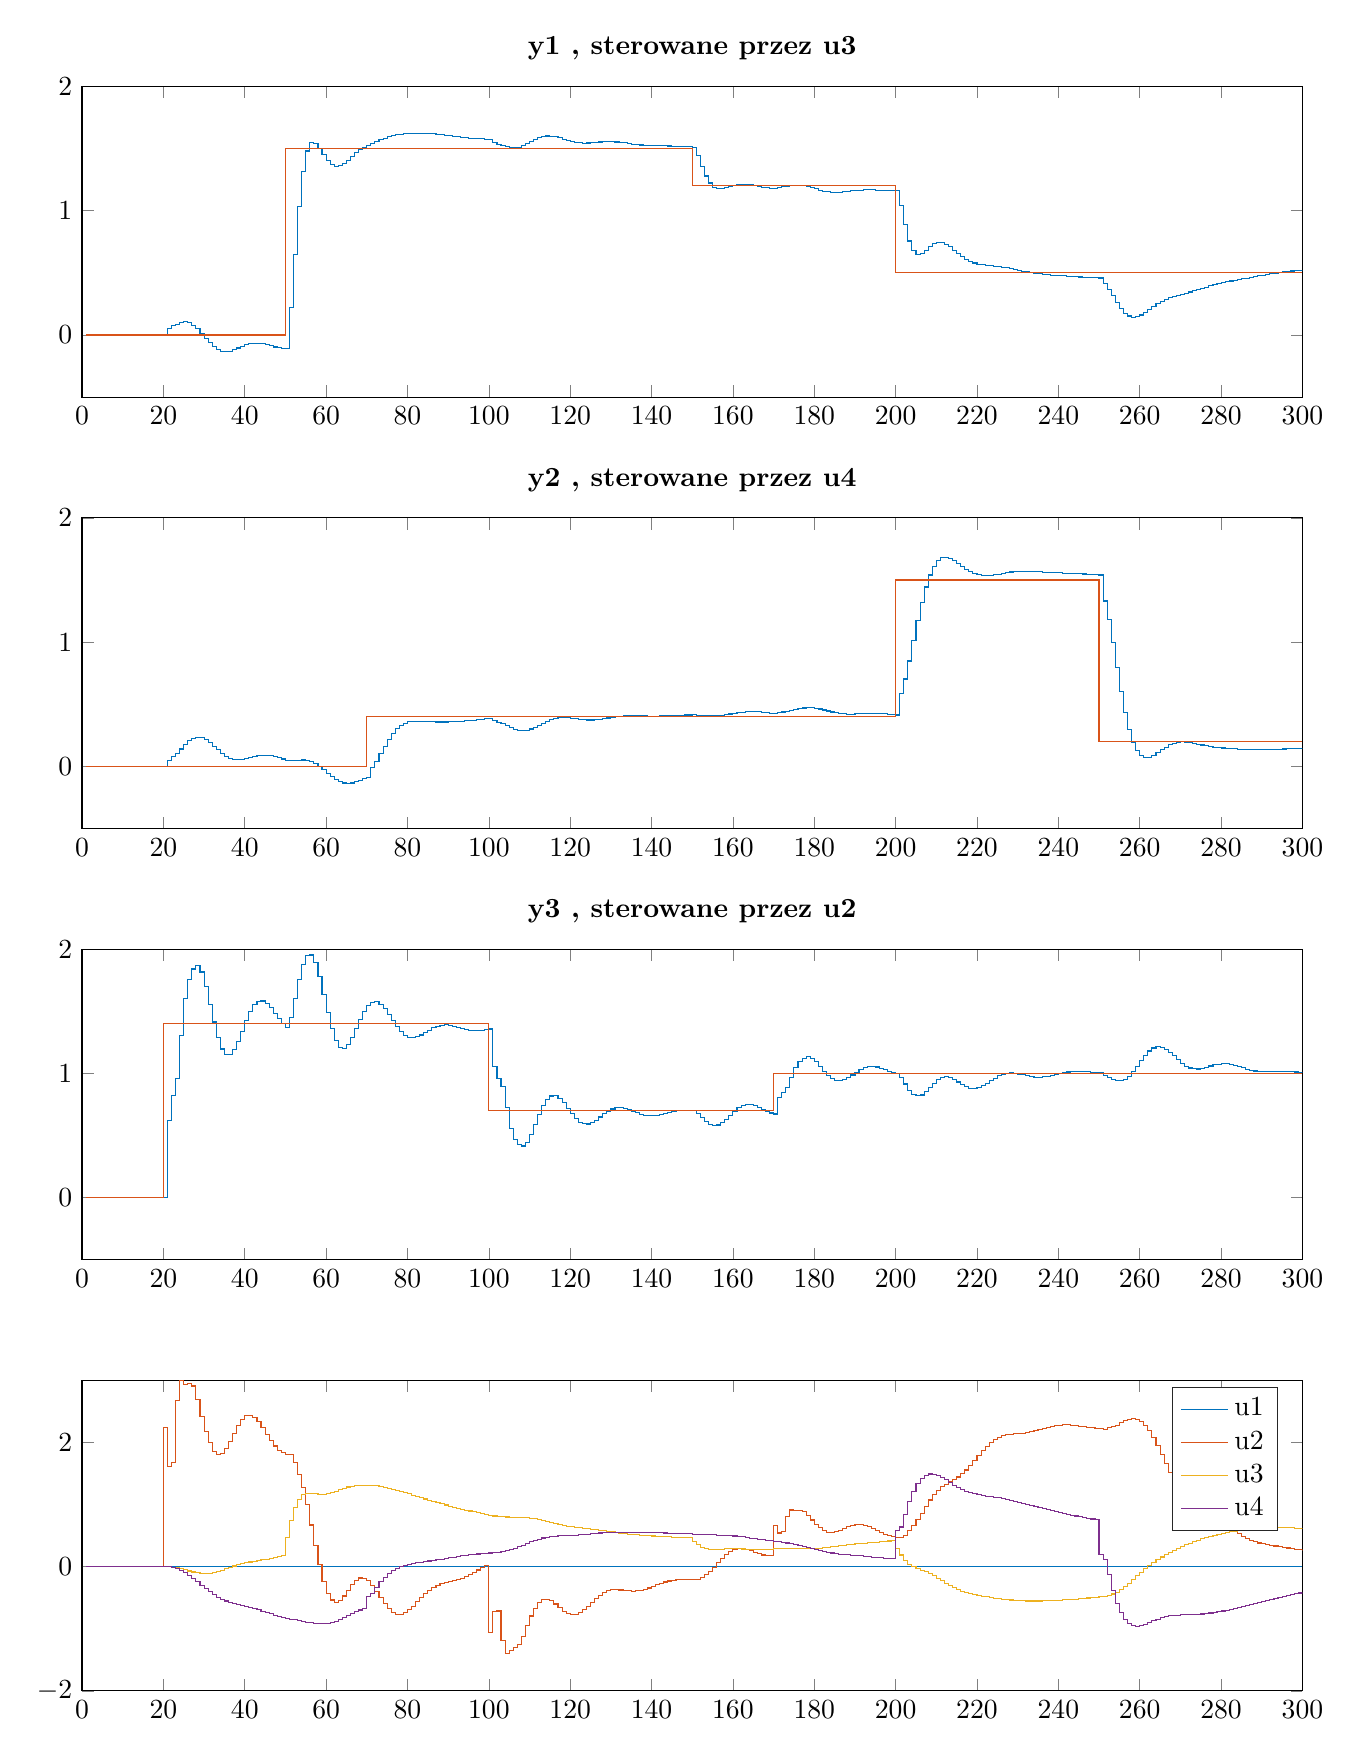
\begin{tikzpicture}

\begin{axis}[%
width=6.102in,
height=1.553in,
at={(1.024in,7.552in)},
scale only axis,
xmin=0,
xmax=300,
ymin=-0.5,
ymax=2,
axis background/.style={fill=white},
title style={font=\bfseries},
title={y1 , sterowane przez u3}
]
\addplot[const plot, color=mycolor1, forget plot] table[row sep=crcr] {%
1	0\\
2	0\\
3	0\\
4	0\\
5	0\\
6	0\\
7	0\\
8	0\\
9	0\\
10	0\\
11	0\\
12	0\\
13	0\\
14	0\\
15	0\\
16	0\\
17	0\\
18	0\\
19	0\\
20	0\\
21	0.0497034640438553\\
22	0.0744770100960698\\
23	0.0825455755979993\\
24	0.0986735257075132\\
25	0.107409757326008\\
26	0.0987339116151879\\
27	0.0779783093220118\\
28	0.0491828826194742\\
29	0.0132146472751859\\
30	-0.0262570352835064\\
31	-0.0637180100720671\\
32	-0.09510479134597\\
33	-0.118032610106792\\
34	-0.131169225501783\\
35	-0.134513290473849\\
36	-0.129531262852872\\
37	-0.118655188195571\\
38	-0.104702569621966\\
39	-0.0904670676153658\\
40	-0.0783505028492368\\
41	-0.070047083536712\\
42	-0.0663885406748046\\
43	-0.0673576724575528\\
44	-0.0722171422036103\\
45	-0.0797185240517569\\
46	-0.0883600729201422\\
47	-0.0966472835367214\\
48	-0.103313771728975\\
49	-0.107476669007462\\
50	-0.108714443636774\\
51	0.223216786844593\\
52	0.649081385976887\\
53	1.03420777287267\\
54	1.31543978113398\\
55	1.4807923344683\\
56	1.54715236264203\\
57	1.54408841747504\\
58	1.50293642402198\\
59	1.44977384905364\\
60	1.4024530925077\\
61	1.37075531591723\\
62	1.35793652396406\\
63	1.36264622805918\\
64	1.38083836887827\\
65	1.40739139259559\\
66	1.43726105148206\\
67	1.46619044210407\\
68	1.4910817795468\\
69	1.5101113372252\\
70	1.52265440068787\\
71	1.54247689949034\\
72	1.5580640839386\\
73	1.57191482333406\\
74	1.58491070290856\\
75	1.59612505509884\\
76	1.60498511477773\\
77	1.6115088530156\\
78	1.61601368502065\\
79	1.61892804022285\\
80	1.62069405244145\\
81	1.62167784637565\\
82	1.62209785290579\\
83	1.62201604833283\\
84	1.62138342411563\\
85	1.6201026531747\\
86	1.61808783084017\\
87	1.61531269385726\\
88	1.61183789886527\\
89	1.60781256617052\\
90	1.60345389127201\\
91	1.59901282414696\\
92	1.59473424624024\\
93	1.59081974734771\\
94	1.58739982252508\\
95	1.58451964352529\\
96	1.58213948006038\\
97	1.58014823414352\\
98	1.57838661403666\\
99	1.57667531348551\\
100	1.57484330462668\\
101	1.54790020169844\\
102	1.53307317926586\\
103	1.52621717849576\\
104	1.5149730770784\\
105	1.50559464926028\\
106	1.50507610019861\\
107	1.51186058526763\\
108	1.52339303208396\\
109	1.53891488954789\\
110	1.55664986115648\\
111	1.57364770271243\\
112	1.5875330558809\\
113	1.5969290654538\\
114	1.60111896697311\\
115	1.60008885586788\\
116	1.59461274092439\\
117	1.58601540553027\\
118	1.57584287129545\\
119	1.56562195170494\\
120	1.55666321443888\\
121	1.54989298712517\\
122	1.54576610708701\\
123	1.54427184252345\\
124	1.54500566844177\\
125	1.5472841622151\\
126	1.55028542177497\\
127	1.55319130926699\\
128	1.55530832285921\\
129	1.55615249174506\\
130	1.55549177970953\\
131	1.55334569002601\\
132	1.54994787107265\\
133	1.5456824908689\\
134	1.54100750175885\\
135	1.53637784130783\\
136	1.53217979668282\\
137	1.5286846065859\\
138	1.52602541719819\\
139	1.52419768933978\\
140	1.5230797092491\\
141	1.52246738473465\\
142	1.52211622518129\\
143	1.52178334093648\\
144	1.52126329748575\\
145	1.52041342319076\\
146	1.5191663303549\\
147	1.51752959761873\\
148	1.51557445271607\\
149	1.51341665191524\\
150	1.51119345147108\\
151	1.44298399828901\\
152	1.35666378849061\\
153	1.27910543133598\\
154	1.22280967496369\\
155	1.1900026388179\\
156	1.17712593650405\\
157	1.1781022801507\\
158	1.18653943574086\\
159	1.19714788579378\\
160	1.20633741401056\\
161	1.21218118235481\\
162	1.21409487219954\\
163	1.212437439313\\
164	1.20811236396777\\
165	1.20222859469311\\
166	1.19585846587853\\
167	1.18988888656031\\
168	1.18494524106345\\
169	1.18137126643617\\
170	1.17925047435271\\
171	1.18910503478083\\
172	1.19466375722904\\
173	1.19732820731562\\
174	1.20202573564203\\
175	1.20576303757464\\
176	1.2053200093692\\
177	1.20124809354127\\
178	1.19463249752712\\
179	1.18587912956718\\
180	1.17589509578759\\
181	1.16612469192301\\
182	1.15776864245859\\
183	1.15157538812755\\
184	1.14796631884692\\
185	1.14700680109949\\
186	1.14836849547623\\
187	1.15143804086891\\
188	1.15547145471377\\
189	1.15971371181204\\
190	1.16350021107444\\
191	1.16634373994832\\
192	1.16798288215157\\
193	1.16838548402061\\
194	1.16771870640343\\
195	1.16629600968559\\
196	1.16450980514441\\
197	1.16276145205949\\
198	1.16140012842873\\
199	1.16067824214863\\
200	1.16072722207585\\
201	1.04424405248716\\
202	0.887848963422581\\
203	0.756484730674978\\
204	0.676753020617231\\
205	0.646687925575911\\
206	0.652741091118308\\
207	0.678400235529275\\
208	0.70865235387536\\
209	0.732685570452863\\
210	0.744756963274598\\
211	0.743494760618803\\
212	0.730540299899322\\
213	0.709198732256919\\
214	0.683311542956036\\
215	0.656423151415606\\
216	0.631289142130869\\
217	0.609689913564024\\
218	0.592455241194785\\
219	0.579615369691404\\
220	0.570617952706146\\
221	0.56456166314808\\
222	0.560409950020774\\
223	0.557164613026655\\
224	0.553990562391058\\
225	0.550289778025484\\
226	0.545727715167544\\
227	0.540219753680652\\
228	0.533887877322848\\
229	0.526998832247698\\
230	0.519895034572747\\
231	0.512928462927983\\
232	0.506405705715685\\
233	0.500549579240496\\
234	0.49547972004127\\
235	0.49121165562579\\
236	0.487671416143014\\
237	0.484721046258671\\
238	0.482189557250986\\
239	0.479903919704903\\
240	0.477715511038657\\
241	0.47551878397883\\
242	0.473260544851079\\
243	0.470939851768705\\
244	0.468599927597173\\
245	0.466314462934492\\
246	0.464171174241234\\
247	0.462255479329291\\
248	0.460636727050252\\
249	0.459358692753543\\
250	0.458435175233744\\
251	0.414334087257967\\
252	0.368049030075664\\
253	0.316443519341206\\
254	0.262119687189393\\
255	0.213219375145983\\
256	0.175762276380571\\
257	0.152470525687524\\
258	0.143554579020711\\
259	0.14739602421497\\
260	0.161124475053179\\
261	0.181298878722367\\
262	0.204588417144481\\
263	0.22823701743573\\
264	0.250280051301479\\
265	0.269591631445135\\
266	0.285807613431009\\
267	0.299153835040079\\
268	0.310230638441873\\
269	0.319803118509438\\
270	0.328625321205269\\
271	0.337312860632183\\
272	0.34627100621656\\
273	0.355676114225569\\
274	0.365500058103016\\
275	0.375563558807845\\
276	0.385603707824856\\
277	0.395341962254325\\
278	0.404541468812805\\
279	0.413046436452945\\
280	0.420800469464462\\
281	0.427844560767516\\
282	0.434298463892028\\
283	0.440331143948968\\
284	0.44612679983993\\
285	0.451852621484748\\
286	0.457633237744361\\
287	0.463535038521666\\
288	0.469561561095264\\
289	0.475659246947841\\
290	0.481731369258073\\
291	0.487656973251253\\
292	0.493311325881205\\
293	0.498584603042415\\
294	0.503396236096925\\
295	0.507703326605506\\
296	0.51150263050036\\
297	0.514826633116862\\
298	0.517735042504815\\
299	0.520303529686632\\
300	0.522611708174249\\
};
\addplot[const plot, color=mycolor2, forget plot] table[row sep=crcr] {%
1	0\\
2	0\\
3	0\\
4	0\\
5	0\\
6	0\\
7	0\\
8	0\\
9	0\\
10	0\\
11	0\\
12	0\\
13	0\\
14	0\\
15	0\\
16	0\\
17	0\\
18	0\\
19	0\\
20	0\\
21	0\\
22	0\\
23	0\\
24	0\\
25	0\\
26	0\\
27	0\\
28	0\\
29	0\\
30	0\\
31	0\\
32	0\\
33	0\\
34	0\\
35	0\\
36	0\\
37	0\\
38	0\\
39	0\\
40	0\\
41	0\\
42	0\\
43	0\\
44	0\\
45	0\\
46	0\\
47	0\\
48	0\\
49	0\\
50	1.5\\
51	1.5\\
52	1.5\\
53	1.5\\
54	1.5\\
55	1.5\\
56	1.5\\
57	1.5\\
58	1.5\\
59	1.5\\
60	1.5\\
61	1.5\\
62	1.5\\
63	1.5\\
64	1.5\\
65	1.5\\
66	1.5\\
67	1.5\\
68	1.5\\
69	1.5\\
70	1.5\\
71	1.5\\
72	1.5\\
73	1.5\\
74	1.5\\
75	1.5\\
76	1.5\\
77	1.5\\
78	1.5\\
79	1.5\\
80	1.5\\
81	1.5\\
82	1.5\\
83	1.5\\
84	1.5\\
85	1.5\\
86	1.5\\
87	1.5\\
88	1.5\\
89	1.5\\
90	1.5\\
91	1.5\\
92	1.5\\
93	1.5\\
94	1.5\\
95	1.5\\
96	1.5\\
97	1.5\\
98	1.5\\
99	1.5\\
100	1.5\\
101	1.5\\
102	1.5\\
103	1.5\\
104	1.5\\
105	1.5\\
106	1.5\\
107	1.5\\
108	1.5\\
109	1.5\\
110	1.5\\
111	1.5\\
112	1.5\\
113	1.5\\
114	1.5\\
115	1.5\\
116	1.5\\
117	1.5\\
118	1.5\\
119	1.5\\
120	1.5\\
121	1.5\\
122	1.5\\
123	1.5\\
124	1.5\\
125	1.5\\
126	1.5\\
127	1.5\\
128	1.5\\
129	1.5\\
130	1.5\\
131	1.5\\
132	1.5\\
133	1.5\\
134	1.5\\
135	1.5\\
136	1.5\\
137	1.5\\
138	1.5\\
139	1.5\\
140	1.5\\
141	1.5\\
142	1.5\\
143	1.5\\
144	1.5\\
145	1.5\\
146	1.5\\
147	1.5\\
148	1.5\\
149	1.5\\
150	1.2\\
151	1.2\\
152	1.2\\
153	1.2\\
154	1.2\\
155	1.2\\
156	1.2\\
157	1.2\\
158	1.2\\
159	1.2\\
160	1.2\\
161	1.2\\
162	1.2\\
163	1.2\\
164	1.2\\
165	1.2\\
166	1.2\\
167	1.2\\
168	1.2\\
169	1.2\\
170	1.2\\
171	1.2\\
172	1.2\\
173	1.2\\
174	1.2\\
175	1.2\\
176	1.2\\
177	1.2\\
178	1.2\\
179	1.2\\
180	1.2\\
181	1.2\\
182	1.2\\
183	1.2\\
184	1.2\\
185	1.2\\
186	1.2\\
187	1.2\\
188	1.2\\
189	1.2\\
190	1.2\\
191	1.2\\
192	1.2\\
193	1.2\\
194	1.2\\
195	1.2\\
196	1.2\\
197	1.2\\
198	1.2\\
199	1.2\\
200	0.5\\
201	0.5\\
202	0.5\\
203	0.5\\
204	0.5\\
205	0.5\\
206	0.5\\
207	0.5\\
208	0.5\\
209	0.5\\
210	0.5\\
211	0.5\\
212	0.5\\
213	0.5\\
214	0.5\\
215	0.5\\
216	0.5\\
217	0.5\\
218	0.5\\
219	0.5\\
220	0.5\\
221	0.5\\
222	0.5\\
223	0.5\\
224	0.5\\
225	0.5\\
226	0.5\\
227	0.5\\
228	0.5\\
229	0.5\\
230	0.5\\
231	0.5\\
232	0.5\\
233	0.5\\
234	0.5\\
235	0.5\\
236	0.5\\
237	0.5\\
238	0.5\\
239	0.5\\
240	0.5\\
241	0.5\\
242	0.5\\
243	0.5\\
244	0.5\\
245	0.5\\
246	0.5\\
247	0.5\\
248	0.5\\
249	0.5\\
250	0.5\\
251	0.5\\
252	0.5\\
253	0.5\\
254	0.5\\
255	0.5\\
256	0.5\\
257	0.5\\
258	0.5\\
259	0.5\\
260	0.5\\
261	0.5\\
262	0.5\\
263	0.5\\
264	0.5\\
265	0.5\\
266	0.5\\
267	0.5\\
268	0.5\\
269	0.5\\
270	0.5\\
271	0.5\\
272	0.5\\
273	0.5\\
274	0.5\\
275	0.5\\
276	0.5\\
277	0.5\\
278	0.5\\
279	0.5\\
280	0.5\\
281	0.5\\
282	0.5\\
283	0.5\\
284	0.5\\
285	0.5\\
286	0.5\\
287	0.5\\
288	0.5\\
289	0.5\\
290	0.5\\
291	0.5\\
292	0.5\\
293	0.5\\
294	0.5\\
295	0.5\\
296	0.5\\
297	0.5\\
298	0.5\\
299	0.5\\
300	0.5\\
};
\end{axis}

\begin{axis}[%
width=6.102in,
height=1.553in,
at={(1.024in,5.395in)},
scale only axis,
xmin=0,
xmax=300,
ymin=-0.5,
ymax=2,
axis background/.style={fill=white},
title style={font=\bfseries},
title={y2 , sterowane przez u4}
]
\addplot[const plot, color=mycolor1, forget plot] table[row sep=crcr] {%
1	0\\
2	0\\
3	0\\
4	0\\
5	0\\
6	0\\
7	0\\
8	0\\
9	0\\
10	0\\
11	0\\
12	0\\
13	0\\
14	0\\
15	0\\
16	0\\
17	0\\
18	0\\
19	0\\
20	0\\
21	0.0458506449378833\\
22	0.0769747791533339\\
23	0.100527978589517\\
24	0.140150185590215\\
25	0.179474855968252\\
26	0.206755621781411\\
27	0.224692772785281\\
28	0.233357821945386\\
29	0.22972251861112\\
30	0.214438931544481\\
31	0.191017941820883\\
32	0.162834919116517\\
33	0.133098050924815\\
34	0.105240739755604\\
35	0.082177268710175\\
36	0.0656752191032073\\
37	0.0563722064742843\\
38	0.0539210472874895\\
39	0.0571030308299431\\
40	0.0640786725219006\\
41	0.07275051085145\\
42	0.0810988016510485\\
43	0.0874426844344256\\
44	0.0906272917009347\\
45	0.0901176541686182\\
46	0.0859877280060923\\
47	0.0788221954890441\\
48	0.0695608479284099\\
49	0.059314589649898\\
50	0.049182083458909\\
51	0.0453278982239228\\
52	0.0474315797369858\\
53	0.050438159554512\\
54	0.0511740567031691\\
55	0.0479005455670313\\
56	0.0386958122792291\\
57	0.0225446773954711\\
58	0.000190306574927402\\
59	-0.0264252702149433\\
60	-0.0547887176105044\\
61	-0.0821038094601481\\
62	-0.105680323096983\\
63	-0.123409892736896\\
64	-0.134061166225808\\
65	-0.137363777524838\\
66	-0.133961903815183\\
67	-0.125252756599186\\
68	-0.113120954867223\\
69	-0.0996257316645649\\
70	-0.0867023814481688\\
71	-0.01237176058136\\
72	0.0412623982322058\\
73	0.100218908915179\\
74	0.162674051501176\\
75	0.219337005609885\\
76	0.26651870807976\\
77	0.303339422098432\\
78	0.330001890918972\\
79	0.347593412748349\\
80	0.357803888384472\\
81	0.362545078965684\\
82	0.363647510593243\\
83	0.362674472132944\\
84	0.360834480517323\\
85	0.358962304009234\\
86	0.357551208363166\\
87	0.356821788315594\\
88	0.356806419343728\\
89	0.35743043444953\\
90	0.358579063021392\\
91	0.360144635418078\\
92	0.36205215804336\\
93	0.364265292900422\\
94	0.366777860720747\\
95	0.369597148359077\\
96	0.372725082225828\\
97	0.376142332779856\\
98	0.37979880237342\\
99	0.383612003389349\\
100	0.387472998138952\\
101	0.368332826995345\\
102	0.356356659863291\\
103	0.34785870887952\\
104	0.330939168690882\\
105	0.312316054223482\\
106	0.29933858945095\\
107	0.291546927599819\\
108	0.288447649326672\\
109	0.291481587951601\\
110	0.300638223277087\\
111	0.31416521440525\\
112	0.330166744772626\\
113	0.346910291653033\\
114	0.362593611494343\\
115	0.375643745087816\\
116	0.385082404749652\\
117	0.390559703879244\\
118	0.392265405780077\\
119	0.390855295967153\\
120	0.387322309627759\\
121	0.382804446873107\\
122	0.378399343898772\\
123	0.375020547117519\\
124	0.373296677394831\\
125	0.373520388331701\\
126	0.375653469722549\\
127	0.379379956575209\\
128	0.384190917501554\\
129	0.389484575908145\\
130	0.39466604464301\\
131	0.399232178035225\\
132	0.402831059638225\\
133	0.405291160406551\\
134	0.406620299413065\\
135	0.406978754788513\\
136	0.406634037357126\\
137	0.405906514112263\\
138	0.405115103183783\\
139	0.404530937945836\\
140	0.404344633702981\\
141	0.404650020520496\\
142	0.405444394323122\\
143	0.406642913676047\\
144	0.408103035226929\\
145	0.409653989184585\\
146	0.411126259587825\\
147	0.412376740311032\\
148	0.41330647960168\\
149	0.413869445990041\\
150	0.414072285182569\\
151	0.412919575416401\\
152	0.410688759182739\\
153	0.40855317283301\\
154	0.407243094208462\\
155	0.407131149733403\\
156	0.408562799803913\\
157	0.411653567777969\\
158	0.416138781022298\\
159	0.421506851496979\\
160	0.427144173710128\\
161	0.43240764601803\\
162	0.436711212421534\\
163	0.439623294807461\\
164	0.440922167657271\\
165	0.440604544566148\\
166	0.43886537201387\\
167	0.436053880661322\\
168	0.432609893524617\\
169	0.428993179363335\\
170	0.425618971970878\\
171	0.432632851186488\\
172	0.437248507184114\\
173	0.441058271986929\\
174	0.449062188859179\\
175	0.458199217311816\\
176	0.465094091625414\\
177	0.469714034182044\\
178	0.472071077627031\\
179	0.471404171066395\\
180	0.467643932632997\\
181	0.461538835688073\\
182	0.453961242892337\\
183	0.445759089311733\\
184	0.437834570792268\\
185	0.430994189465443\\
186	0.425772991046072\\
187	0.422406017025393\\
188	0.420858679306778\\
189	0.420857309618493\\
190	0.421949261328613\\
191	0.423594446518319\\
192	0.425256410505132\\
193	0.426475891603035\\
194	0.426924556021497\\
195	0.426434610252503\\
196	0.425000824447601\\
197	0.422758331124031\\
198	0.419943624309463\\
199	0.416846605508913\\
200	0.413761485897377\\
201	0.583250936680693\\
202	0.703005794888033\\
203	0.848357653464694\\
204	1.01535355309382\\
205	1.17731439365025\\
206	1.32201917937697\\
207	1.44408720812415\\
208	1.54038953329714\\
209	1.61023255479839\\
210	1.65519657128762\\
211	1.67837259450896\\
212	1.6836900105904\\
213	1.67546367418824\\
214	1.65802789463815\\
215	1.6354128538251\\
216	1.6111051546221\\
217	1.58790329150505\\
218	1.56784628751454\\
219	1.55220513155311\\
220	1.54153477296076\\
221	1.53577559905335\\
222	1.53438762728195\\
223	1.53650201146916\\
224	1.54107535502138\\
225	1.5470324370959\\
226	1.55338529734563\\
227	1.5593207245312\\
228	1.56425242533993\\
229	1.56783817890838\\
230	1.56996603013292\\
231	1.57071650285763\\
232	1.57030950391395\\
233	1.56904501456706\\
234	1.56724596234479\\
235	1.56521003225749\\
236	1.56317492325023\\
237	1.56129906682041\\
238	1.55965746107486\\
239	1.55825032402387\\
240	1.557020933313\\
241	1.55587838766576\\
242	1.55472107913613\\
243	1.5534572932773\\
244	1.55202038220103\\
245	1.55037717871396\\
246	1.54852953589175\\
247	1.54650991386962\\
248	1.54437267343663\\
249	1.54218311404272\\
250	1.54000631235799\\
251	1.33137530863735\\
252	1.17981443044635\\
253	0.999397281744063\\
254	0.796554154527414\\
255	0.603520125860317\\
256	0.435357944342728\\
257	0.29845190146813\\
258	0.195553578556043\\
259	0.125953136481244\\
260	0.0860731338585585\\
261	0.0705585308843382\\
262	0.0732865144693624\\
263	0.0881405888827837\\
264	0.109564844893676\\
265	0.132942620934192\\
266	0.154803435042374\\
267	0.172861361847654\\
268	0.185921981859955\\
269	0.193704359928032\\
270	0.196614737200769\\
271	0.195504473667074\\
272	0.191442652831388\\
273	0.185525694255384\\
274	0.178736113012223\\
275	0.171854431405442\\
276	0.165421643565711\\
277	0.159744081985063\\
278	0.15492900210668\\
279	0.150938047183571\\
280	0.147646455552474\\
281	0.14489790304719\\
282	0.142547824286306\\
283	0.140491394005747\\
284	0.138675515133251\\
285	0.137096750664801\\
286	0.135788916662749\\
287	0.134804924365069\\
288	0.134197458399818\\
289	0.134002366635824\\
290	0.13422745187666\\
291	0.134847958315117\\
292	0.135808684747433\\
293	0.137031534685422\\
294	0.138426564475173\\
295	0.139904270148966\\
296	0.141386944395625\\
297	0.142817359837708\\
298	0.144163677904384\\
299	0.145420212357928\\
300	0.146604367683369\\
};
\addplot[const plot, color=mycolor2, forget plot] table[row sep=crcr] {%
1	0\\
2	0\\
3	0\\
4	0\\
5	0\\
6	0\\
7	0\\
8	0\\
9	0\\
10	0\\
11	0\\
12	0\\
13	0\\
14	0\\
15	0\\
16	0\\
17	0\\
18	0\\
19	0\\
20	0\\
21	0\\
22	0\\
23	0\\
24	0\\
25	0\\
26	0\\
27	0\\
28	0\\
29	0\\
30	0\\
31	0\\
32	0\\
33	0\\
34	0\\
35	0\\
36	0\\
37	0\\
38	0\\
39	0\\
40	0\\
41	0\\
42	0\\
43	0\\
44	0\\
45	0\\
46	0\\
47	0\\
48	0\\
49	0\\
50	0\\
51	0\\
52	0\\
53	0\\
54	0\\
55	0\\
56	0\\
57	0\\
58	0\\
59	0\\
60	0\\
61	0\\
62	0\\
63	0\\
64	0\\
65	0\\
66	0\\
67	0\\
68	0\\
69	0\\
70	0.4\\
71	0.4\\
72	0.4\\
73	0.4\\
74	0.4\\
75	0.4\\
76	0.4\\
77	0.4\\
78	0.4\\
79	0.4\\
80	0.4\\
81	0.4\\
82	0.4\\
83	0.4\\
84	0.4\\
85	0.4\\
86	0.4\\
87	0.4\\
88	0.4\\
89	0.4\\
90	0.4\\
91	0.4\\
92	0.4\\
93	0.4\\
94	0.4\\
95	0.4\\
96	0.4\\
97	0.4\\
98	0.4\\
99	0.4\\
100	0.4\\
101	0.4\\
102	0.4\\
103	0.4\\
104	0.4\\
105	0.4\\
106	0.4\\
107	0.4\\
108	0.4\\
109	0.4\\
110	0.4\\
111	0.4\\
112	0.4\\
113	0.4\\
114	0.4\\
115	0.4\\
116	0.4\\
117	0.4\\
118	0.4\\
119	0.4\\
120	0.4\\
121	0.4\\
122	0.4\\
123	0.4\\
124	0.4\\
125	0.4\\
126	0.4\\
127	0.4\\
128	0.4\\
129	0.4\\
130	0.4\\
131	0.4\\
132	0.4\\
133	0.4\\
134	0.4\\
135	0.4\\
136	0.4\\
137	0.4\\
138	0.4\\
139	0.4\\
140	0.4\\
141	0.4\\
142	0.4\\
143	0.4\\
144	0.4\\
145	0.4\\
146	0.4\\
147	0.4\\
148	0.4\\
149	0.4\\
150	0.4\\
151	0.4\\
152	0.4\\
153	0.4\\
154	0.4\\
155	0.4\\
156	0.4\\
157	0.4\\
158	0.4\\
159	0.4\\
160	0.4\\
161	0.4\\
162	0.4\\
163	0.4\\
164	0.4\\
165	0.4\\
166	0.4\\
167	0.4\\
168	0.4\\
169	0.4\\
170	0.4\\
171	0.4\\
172	0.4\\
173	0.4\\
174	0.4\\
175	0.4\\
176	0.4\\
177	0.4\\
178	0.4\\
179	0.4\\
180	0.4\\
181	0.4\\
182	0.4\\
183	0.4\\
184	0.4\\
185	0.4\\
186	0.4\\
187	0.4\\
188	0.4\\
189	0.4\\
190	0.4\\
191	0.4\\
192	0.4\\
193	0.4\\
194	0.4\\
195	0.4\\
196	0.4\\
197	0.4\\
198	0.4\\
199	0.4\\
200	1.5\\
201	1.5\\
202	1.5\\
203	1.5\\
204	1.5\\
205	1.5\\
206	1.5\\
207	1.5\\
208	1.5\\
209	1.5\\
210	1.5\\
211	1.5\\
212	1.5\\
213	1.5\\
214	1.5\\
215	1.5\\
216	1.5\\
217	1.5\\
218	1.5\\
219	1.5\\
220	1.5\\
221	1.5\\
222	1.5\\
223	1.5\\
224	1.5\\
225	1.5\\
226	1.5\\
227	1.5\\
228	1.5\\
229	1.5\\
230	1.5\\
231	1.5\\
232	1.5\\
233	1.5\\
234	1.5\\
235	1.5\\
236	1.5\\
237	1.5\\
238	1.5\\
239	1.5\\
240	1.5\\
241	1.5\\
242	1.5\\
243	1.5\\
244	1.5\\
245	1.5\\
246	1.5\\
247	1.5\\
248	1.5\\
249	1.5\\
250	0.2\\
251	0.2\\
252	0.2\\
253	0.2\\
254	0.2\\
255	0.2\\
256	0.2\\
257	0.2\\
258	0.2\\
259	0.2\\
260	0.2\\
261	0.2\\
262	0.2\\
263	0.2\\
264	0.2\\
265	0.2\\
266	0.2\\
267	0.2\\
268	0.2\\
269	0.2\\
270	0.2\\
271	0.2\\
272	0.2\\
273	0.2\\
274	0.2\\
275	0.2\\
276	0.2\\
277	0.2\\
278	0.2\\
279	0.2\\
280	0.2\\
281	0.2\\
282	0.2\\
283	0.2\\
284	0.2\\
285	0.2\\
286	0.2\\
287	0.2\\
288	0.2\\
289	0.2\\
290	0.2\\
291	0.2\\
292	0.2\\
293	0.2\\
294	0.2\\
295	0.2\\
296	0.2\\
297	0.2\\
298	0.2\\
299	0.2\\
300	0.2\\
};
\end{axis}

\begin{axis}[%
width=6.102in,
height=1.553in,
at={(1.024in,3.239in)},
scale only axis,
xmin=0,
xmax=300,
ymin=-0.5,
ymax=2,
axis background/.style={fill=white},
title style={font=\bfseries},
title={y3 , sterowane przez u2}
]
\addplot[const plot, color=mycolor1, forget plot] table[row sep=crcr] {%
1	0\\
2	0\\
3	0\\
4	0\\
5	0\\
6	0\\
7	0\\
8	0\\
9	0\\
10	0\\
11	0\\
12	0\\
13	0\\
14	0\\
15	0\\
16	0\\
17	0\\
18	0\\
19	0\\
20	0\\
21	0.618887925337999\\
22	0.82074244791471\\
23	0.955014702843231\\
24	1.3075777303199\\
25	1.60312193758783\\
26	1.75370525918019\\
27	1.83933998788434\\
28	1.86933802260971\\
29	1.81569273359772\\
30	1.69796882736472\\
31	1.55582774897945\\
32	1.41330181027844\\
33	1.28737859549445\\
34	1.19582781940321\\
35	1.14962501296319\\
36	1.14923210869915\\
37	1.18820688858068\\
38	1.25604494466253\\
39	1.33933676353634\\
40	1.42389250405742\\
41	1.49733408011968\\
42	1.55071805718211\\
43	1.57921639658948\\
44	1.58225319648709\\
45	1.56306209254805\\
46	1.52767872497921\\
47	1.48364442623792\\
48	1.43869666029275\\
49	1.39961620116827\\
50	1.371363788982\\
51	1.44784828382849\\
52	1.60088994699681\\
53	1.75431240498476\\
54	1.87397620451248\\
55	1.94546399622374\\
56	1.95237679720191\\
57	1.89158716188266\\
58	1.77883430530029\\
59	1.6374566475818\\
60	1.49082056385241\\
61	1.36058075977789\\
62	1.26388181337328\\
63	1.21023696245024\\
64	1.20098243771746\\
65	1.23062647505492\\
66	1.28867587562144\\
67	1.36179968915815\\
68	1.43626455962824\\
69	1.50011132038043\\
70	1.54467828167095\\
71	1.57192738827885\\
72	1.57474070629995\\
73	1.5547997541353\\
74	1.51939684926368\\
75	1.47412161082947\\
76	1.42441461764414\\
77	1.37679231748501\\
78	1.33680171391917\\
79	1.30782183051361\\
80	1.29138837353546\\
81	1.2874120495593\\
82	1.29420205530865\\
83	1.30886414141035\\
84	1.32793954488803\\
85	1.34795981031497\\
86	1.36588667458663\\
87	1.37946593642264\\
88	1.38743526043285\\
89	1.38954979583553\\
90	1.38645807834838\\
91	1.37947535339229\\
92	1.37029551344252\\
93	1.36068853085511\\
94	1.35223112625765\\
95	1.34610549126129\\
96	1.34298438501826\\
97	1.34300666812421\\
98	1.34583428902364\\
99	1.35077081593958\\
100	1.35691527934317\\
101	1.05387986420911\\
102	0.958783280178007\\
103	0.89626901231526\\
104	0.723043100605647\\
105	0.557496582235451\\
106	0.470531087469466\\
107	0.428147988192221\\
108	0.41536130871737\\
109	0.444836476387257\\
110	0.510003897593927\\
111	0.589764979325588\\
112	0.669343467892391\\
113	0.739414421975993\\
114	0.790893205507272\\
115	0.817711422143093\\
116	0.819363977007382\\
117	0.799408088221532\\
118	0.76366224418706\\
119	0.719421352560644\\
120	0.674408585072091\\
121	0.635404820105923\\
122	0.607312288561555\\
123	0.592769075424813\\
124	0.592093478873952\\
125	0.603527518703048\\
126	0.623778763025072\\
127	0.648728167636483\\
128	0.674148650885188\\
129	0.696334878406274\\
130	0.712574224848449\\
131	0.721407907378965\\
132	0.722669736602359\\
133	0.717329652133805\\
134	0.707193262772487\\
135	0.69452063864091\\
136	0.681631173366129\\
137	0.670554775939963\\
138	0.662774187199012\\
139	0.659083377468351\\
140	0.659566618066931\\
141	0.663684559268708\\
142	0.670439797058142\\
143	0.678586562400525\\
144	0.686847646088425\\
145	0.694105752848054\\
146	0.699544785189411\\
147	0.70272730975043\\
148	0.703605735114297\\
149	0.70247479415865\\
150	0.69988047156992\\
151	0.678255859877598\\
152	0.643995583930507\\
153	0.612589843105156\\
154	0.590650346523083\\
155	0.580470564882355\\
156	0.584505186257977\\
157	0.602473342167735\\
158	0.630383915691314\\
159	0.662904053632771\\
160	0.694946329879306\\
161	0.722042621105486\\
162	0.740885522622136\\
163	0.749898932938031\\
164	0.749270938146063\\
165	0.740599492481971\\
166	0.726447866696101\\
167	0.709848834116189\\
168	0.693777684213529\\
169	0.680702773628419\\
170	0.672291006761152\\
171	0.801895890339512\\
172	0.847357794657119\\
173	0.882624546951897\\
174	0.967507573357544\\
175	1.04956424249036\\
176	1.09686642613095\\
177	1.12280941725762\\
178	1.1331284015469\\
179	1.12222917463164\\
180	1.09323405855802\\
181	1.05585410911209\\
182	1.01730428276047\\
183	0.982517574485513\\
184	0.956233378006455\\
185	0.941696393325839\\
186	0.939498799722109\\
187	0.948205889034596\\
188	0.965154692350451\\
189	0.986851384392597\\
190	1.00950208902114\\
191	1.02968758242026\\
192	1.04484403194059\\
193	1.0534892239738\\
194	1.05528261373443\\
195	1.05093050412308\\
196	1.04193902454443\\
197	1.0302771747509\\
198	1.01802402368898\\
199	1.0070508581003\\
200	0.998775757055636\\
201	0.969379834511916\\
202	0.913751395476984\\
203	0.861740469236826\\
204	0.830546638715308\\
205	0.818988601504749\\
206	0.825964837115807\\
207	0.850258604214879\\
208	0.884902794026589\\
209	0.920536116262771\\
210	0.949981576384736\\
211	0.968723118743756\\
212	0.974541978304818\\
213	0.967900408950918\\
214	0.951731186897551\\
215	0.93039078921341\\
216	0.908598793434963\\
217	0.890643252621949\\
218	0.879736763924137\\
219	0.877588450832254\\
220	0.884306392058762\\
221	0.898591161577283\\
222	0.918114957024891\\
223	0.940004340068921\\
224	0.961348124338345\\
225	0.979645567340416\\
226	0.993130735314292\\
227	1.0009426572755\\
228	1.00313816390134\\
229	1.00056615538958\\
230	0.994640465631286\\
231	0.987059218137822\\
232	0.979519663423446\\
233	0.973471121963221\\
234	0.969937282796892\\
235	0.969424681028345\\
236	0.971919117610428\\
237	0.976958572675684\\
238	0.983761515725632\\
239	0.99138428431547\\
240	0.99888054057499\\
241	1.00543921473343\\
242	1.01048374385176\\
243	1.01372344747599\\
244	1.01515614687582\\
245	1.01502839045035\\
246	1.0137649692574\\
247	1.01188227978551\\
248	1.00990043462346\\
249	1.00826713630679\\
250	1.00730280041112\\
251	0.985967274186083\\
252	0.966232853098963\\
253	0.953264540719062\\
254	0.9425379697614\\
255	0.939566111979033\\
256	0.950728404212149\\
257	0.975690287633946\\
258	1.01142584335584\\
259	1.05471725057776\\
260	1.10096469172367\\
261	1.14444316947968\\
262	1.17999800186616\\
263	1.20395671253209\\
264	1.21430748949875\\
265	1.21086238504349\\
266	1.19525735906339\\
267	1.17056038101391\\
268	1.14066503666265\\
269	1.10967285227805\\
270	1.08132121395291\\
271	1.05850811145169\\
272	1.04299045512766\\
273	1.0352887109892\\
274	1.03477870420907\\
275	1.03993121545884\\
276	1.04864924208105\\
277	1.05864234059419\\
278	1.06777793887792\\
279	1.07436200108606\\
280	1.07731866407077\\
281	1.07625666011148\\
282	1.07142822278212\\
283	1.06360121896646\\
284	1.05387504462802\\
285	1.04347469062539\\
286	1.03355579742503\\
287	1.025047412915\\
288	1.01854997646587\\
289	1.01429556745244\\
290	1.01216741609548\\
291	1.01176747043197\\
292	1.01251537929389\\
293	1.01376000240428\\
294	1.01488538380732\\
295	1.01539647273829\\
296	1.01497490495542\\
297	1.01350089890214\\
298	1.01104283592864\\
299	1.00782060650263\\
300	1.00415179440765\\
};
\addplot[const plot, color=mycolor2, forget plot] table[row sep=crcr] {%
1	0\\
2	0\\
3	0\\
4	0\\
5	0\\
6	0\\
7	0\\
8	0\\
9	0\\
10	0\\
11	0\\
12	0\\
13	0\\
14	0\\
15	0\\
16	0\\
17	0\\
18	0\\
19	0\\
20	1.4\\
21	1.4\\
22	1.4\\
23	1.4\\
24	1.4\\
25	1.4\\
26	1.4\\
27	1.4\\
28	1.4\\
29	1.4\\
30	1.4\\
31	1.4\\
32	1.4\\
33	1.4\\
34	1.4\\
35	1.4\\
36	1.4\\
37	1.4\\
38	1.4\\
39	1.4\\
40	1.4\\
41	1.4\\
42	1.4\\
43	1.4\\
44	1.4\\
45	1.4\\
46	1.4\\
47	1.4\\
48	1.4\\
49	1.4\\
50	1.4\\
51	1.4\\
52	1.4\\
53	1.4\\
54	1.4\\
55	1.4\\
56	1.4\\
57	1.4\\
58	1.4\\
59	1.4\\
60	1.4\\
61	1.4\\
62	1.4\\
63	1.4\\
64	1.4\\
65	1.4\\
66	1.4\\
67	1.4\\
68	1.4\\
69	1.4\\
70	1.4\\
71	1.4\\
72	1.4\\
73	1.4\\
74	1.4\\
75	1.4\\
76	1.4\\
77	1.4\\
78	1.4\\
79	1.4\\
80	1.4\\
81	1.4\\
82	1.4\\
83	1.4\\
84	1.4\\
85	1.4\\
86	1.4\\
87	1.4\\
88	1.4\\
89	1.4\\
90	1.4\\
91	1.4\\
92	1.4\\
93	1.4\\
94	1.4\\
95	1.4\\
96	1.4\\
97	1.4\\
98	1.4\\
99	1.4\\
100	0.7\\
101	0.7\\
102	0.7\\
103	0.7\\
104	0.7\\
105	0.7\\
106	0.7\\
107	0.7\\
108	0.7\\
109	0.7\\
110	0.7\\
111	0.7\\
112	0.7\\
113	0.7\\
114	0.7\\
115	0.7\\
116	0.7\\
117	0.7\\
118	0.7\\
119	0.7\\
120	0.7\\
121	0.7\\
122	0.7\\
123	0.7\\
124	0.7\\
125	0.7\\
126	0.7\\
127	0.7\\
128	0.7\\
129	0.7\\
130	0.7\\
131	0.7\\
132	0.7\\
133	0.7\\
134	0.7\\
135	0.7\\
136	0.7\\
137	0.7\\
138	0.7\\
139	0.7\\
140	0.7\\
141	0.7\\
142	0.7\\
143	0.7\\
144	0.7\\
145	0.7\\
146	0.7\\
147	0.7\\
148	0.7\\
149	0.7\\
150	0.7\\
151	0.7\\
152	0.7\\
153	0.7\\
154	0.7\\
155	0.7\\
156	0.7\\
157	0.7\\
158	0.7\\
159	0.7\\
160	0.7\\
161	0.7\\
162	0.7\\
163	0.7\\
164	0.7\\
165	0.7\\
166	0.7\\
167	0.7\\
168	0.7\\
169	0.7\\
170	1\\
171	1\\
172	1\\
173	1\\
174	1\\
175	1\\
176	1\\
177	1\\
178	1\\
179	1\\
180	1\\
181	1\\
182	1\\
183	1\\
184	1\\
185	1\\
186	1\\
187	1\\
188	1\\
189	1\\
190	1\\
191	1\\
192	1\\
193	1\\
194	1\\
195	1\\
196	1\\
197	1\\
198	1\\
199	1\\
200	1\\
201	1\\
202	1\\
203	1\\
204	1\\
205	1\\
206	1\\
207	1\\
208	1\\
209	1\\
210	1\\
211	1\\
212	1\\
213	1\\
214	1\\
215	1\\
216	1\\
217	1\\
218	1\\
219	1\\
220	1\\
221	1\\
222	1\\
223	1\\
224	1\\
225	1\\
226	1\\
227	1\\
228	1\\
229	1\\
230	1\\
231	1\\
232	1\\
233	1\\
234	1\\
235	1\\
236	1\\
237	1\\
238	1\\
239	1\\
240	1\\
241	1\\
242	1\\
243	1\\
244	1\\
245	1\\
246	1\\
247	1\\
248	1\\
249	1\\
250	1\\
251	1\\
252	1\\
253	1\\
254	1\\
255	1\\
256	1\\
257	1\\
258	1\\
259	1\\
260	1\\
261	1\\
262	1\\
263	1\\
264	1\\
265	1\\
266	1\\
267	1\\
268	1\\
269	1\\
270	1\\
271	1\\
272	1\\
273	1\\
274	1\\
275	1\\
276	1\\
277	1\\
278	1\\
279	1\\
280	1\\
281	1\\
282	1\\
283	1\\
284	1\\
285	1\\
286	1\\
287	1\\
288	1\\
289	1\\
290	1\\
291	1\\
292	1\\
293	1\\
294	1\\
295	1\\
296	1\\
297	1\\
298	1\\
299	1\\
300	1\\
};
\end{axis}

\begin{axis}[%
width=6.102in,
height=1.553in,
at={(1.024in,1.083in)},
scale only axis,
xmin=0,
xmax=300,
ymin=-2,
ymax=3,
axis background/.style={fill=white},
legend style={legend cell align=left, align=left, draw=white!15!black}
]
\addplot[const plot, color=mycolor1] table[row sep=crcr] {%
1	0\\
2	0\\
3	0\\
4	0\\
5	0\\
6	0\\
7	0\\
8	0\\
9	0\\
10	0\\
11	0\\
12	0\\
13	0\\
14	0\\
15	0\\
16	0\\
17	0\\
18	0\\
19	0\\
20	0\\
21	0\\
22	0\\
23	0\\
24	0\\
25	0\\
26	0\\
27	0\\
28	0\\
29	0\\
30	0\\
31	0\\
32	0\\
33	0\\
34	0\\
35	0\\
36	0\\
37	0\\
38	0\\
39	0\\
40	0\\
41	0\\
42	0\\
43	0\\
44	0\\
45	0\\
46	0\\
47	0\\
48	0\\
49	0\\
50	0\\
51	0\\
52	0\\
53	0\\
54	0\\
55	0\\
56	0\\
57	0\\
58	0\\
59	0\\
60	0\\
61	0\\
62	0\\
63	0\\
64	0\\
65	0\\
66	0\\
67	0\\
68	0\\
69	0\\
70	0\\
71	0\\
72	0\\
73	0\\
74	0\\
75	0\\
76	0\\
77	0\\
78	0\\
79	0\\
80	0\\
81	0\\
82	0\\
83	0\\
84	0\\
85	0\\
86	0\\
87	0\\
88	0\\
89	0\\
90	0\\
91	0\\
92	0\\
93	0\\
94	0\\
95	0\\
96	0\\
97	0\\
98	0\\
99	0\\
100	0\\
101	0\\
102	0\\
103	0\\
104	0\\
105	0\\
106	0\\
107	0\\
108	0\\
109	0\\
110	0\\
111	0\\
112	0\\
113	0\\
114	0\\
115	0\\
116	0\\
117	0\\
118	0\\
119	0\\
120	0\\
121	0\\
122	0\\
123	0\\
124	0\\
125	0\\
126	0\\
127	0\\
128	0\\
129	0\\
130	0\\
131	0\\
132	0\\
133	0\\
134	0\\
135	0\\
136	0\\
137	0\\
138	0\\
139	0\\
140	0\\
141	0\\
142	0\\
143	0\\
144	0\\
145	0\\
146	0\\
147	0\\
148	0\\
149	0\\
150	0\\
151	0\\
152	0\\
153	0\\
154	0\\
155	0\\
156	0\\
157	0\\
158	0\\
159	0\\
160	0\\
161	0\\
162	0\\
163	0\\
164	0\\
165	0\\
166	0\\
167	0\\
168	0\\
169	0\\
170	0\\
171	0\\
172	0\\
173	0\\
174	0\\
175	0\\
176	0\\
177	0\\
178	0\\
179	0\\
180	0\\
181	0\\
182	0\\
183	0\\
184	0\\
185	0\\
186	0\\
187	0\\
188	0\\
189	0\\
190	0\\
191	0\\
192	0\\
193	0\\
194	0\\
195	0\\
196	0\\
197	0\\
198	0\\
199	0\\
200	0\\
201	0\\
202	0\\
203	0\\
204	0\\
205	0\\
206	0\\
207	0\\
208	0\\
209	0\\
210	0\\
211	0\\
212	0\\
213	0\\
214	0\\
215	0\\
216	0\\
217	0\\
218	0\\
219	0\\
220	0\\
221	0\\
222	0\\
223	0\\
224	0\\
225	0\\
226	0\\
227	0\\
228	0\\
229	0\\
230	0\\
231	0\\
232	0\\
233	0\\
234	0\\
235	0\\
236	0\\
237	0\\
238	0\\
239	0\\
240	0\\
241	0\\
242	0\\
243	0\\
244	0\\
245	0\\
246	0\\
247	0\\
248	0\\
249	0\\
250	0\\
251	0\\
252	0\\
253	0\\
254	0\\
255	0\\
256	0\\
257	0\\
258	0\\
259	0\\
260	0\\
261	0\\
262	0\\
263	0\\
264	0\\
265	0\\
266	0\\
267	0\\
268	0\\
269	0\\
270	0\\
271	0\\
272	0\\
273	0\\
274	0\\
275	0\\
276	0\\
277	0\\
278	0\\
279	0\\
280	0\\
281	0\\
282	0\\
283	0\\
284	0\\
285	0\\
286	0\\
287	0\\
288	0\\
289	0\\
290	0\\
291	0\\
292	0\\
293	0\\
294	0\\
295	0\\
296	0\\
297	0\\
298	0\\
299	0\\
300	0\\
};
\addlegendentry{u1}

\addplot[const plot, color=mycolor2] table[row sep=crcr] {%
1	0\\
2	0\\
3	0\\
4	0\\
5	0\\
6	0\\
7	0\\
8	0\\
9	0\\
10	0\\
11	0\\
12	0\\
13	0\\
14	0\\
15	0\\
16	0\\
17	0\\
18	0\\
19	0\\
20	2.247\\
21	1.617\\
22	1.67368487983251\\
23	2.67820793749899\\
24	3\\
25	2.92900201968175\\
26	2.94704590224879\\
27	2.9076712666237\\
28	2.68564856857924\\
29	2.41075840637673\\
30	2.18085321995414\\
31	1.99365619244543\\
32	1.85704731525064\\
33	1.79836134106886\\
34	1.81946061664712\\
35	1.89975780791192\\
36	2.01718151638628\\
37	2.15015000027963\\
38	2.27519991192858\\
39	2.37193440133953\\
40	2.42762299084838\\
41	2.43735863730837\\
42	2.40303241831068\\
43	2.33248046631043\\
44	2.23776286114993\\
45	2.132674507161\\
46	2.03043049149497\\
47	1.94189490230509\\
48	1.87435086696782\\
49	1.83091755314184\\
50	1.81068187568286\\
51	1.80941829541624\\
52	1.6742349448276\\
53	1.48449825638687\\
54	1.27123774687059\\
55	0.997549994475563\\
56	0.670926494827894\\
57	0.336518802143647\\
58	0.0280989301034024\\
59	-0.232570668876987\\
60	-0.425088685112873\\
61	-0.537483445675733\\
62	-0.572527283500717\\
63	-0.544048809244158\\
64	-0.471898919228172\\
65	-0.379096949977385\\
66	-0.288517887871437\\
67	-0.219084187266945\\
68	-0.183295534029623\\
69	-0.186412841758669\\
70	-0.226727467923015\\
71	-0.296724818176981\\
72	-0.395487991987263\\
73	-0.496249980690779\\
74	-0.591924300566155\\
75	-0.675131596446272\\
76	-0.734495961553064\\
77	-0.764637731733768\\
78	-0.766163295033868\\
79	-0.7417193746154\\
80	-0.695796671467867\\
81	-0.635063205989815\\
82	-0.566942634533459\\
83	-0.498171219702018\\
84	-0.434207402477523\\
85	-0.378877027794914\\
86	-0.334073728297967\\
87	-0.29979188467788\\
88	-0.274489368738653\\
89	-0.255584471888814\\
90	-0.239991557722505\\
91	-0.224654255549046\\
92	-0.207000601740409\\
93	-0.185252743612537\\
94	-0.15857097958137\\
95	-0.12704162244867\\
96	-0.0915322084896999\\
97	-0.0534527134112361\\
98	-0.0144720940516196\\
99	0.0237613130387817\\
100	-1.06364438434973\\
101	-0.715660527768031\\
102	-0.71460178990095\\
103	-1.19102416884872\\
104	-1.39889212989985\\
105	-1.34308342227766\\
106	-1.30253467979927\\
107	-1.25473331942068\\
108	-1.11896535440199\\
109	-0.94541344412171\\
110	-0.794586085139729\\
111	-0.672436952263011\\
112	-0.579755506189769\\
113	-0.529089416755686\\
114	-0.523066712698996\\
115	-0.551165831848371\\
116	-0.600604433441784\\
117	-0.659358490643303\\
118	-0.714869206060402\\
119	-0.756000259094245\\
120	-0.775635324015508\\
121	-0.771044916568563\\
122	-0.743265633588195\\
123	-0.696535253498329\\
124	-0.637388650688265\\
125	-0.573332980556834\\
126	-0.511565439499029\\
127	-0.457993477868249\\
128	-0.41656985135194\\
129	-0.38897656715978\\
130	-0.374692370596568\\
131	-0.371384207415661\\
132	-0.375505720782866\\
133	-0.382986468184018\\
134	-0.389903739995685\\
135	-0.393040175533388\\
136	-0.390259228115154\\
137	-0.380669264287705\\
138	-0.364582384773043\\
139	-0.343302298710188\\
140	-0.318795895980877\\
141	-0.293313001919655\\
142	-0.269017372380408\\
143	-0.24768141904185\\
144	-0.230480539862659\\
145	-0.217903382571273\\
146	-0.209775078061317\\
147	-0.205374311493679\\
148	-0.203614013496546\\
149	-0.203250339045152\\
150	-0.203085369710421\\
151	-0.202134706721273\\
152	-0.170450745739012\\
153	-0.125104431782917\\
154	-0.0738072368426174\\
155	-0.0107236161476776\\
156	0.06129977759489\\
157	0.132255548656378\\
158	0.194879314378479\\
159	0.244789624339044\\
160	0.278299554402814\\
161	0.293717826332295\\
162	0.292469263000639\\
163	0.278209989708718\\
164	0.255690806005083\\
165	0.230090630321744\\
166	0.206301503252702\\
167	0.188159508480634\\
168	0.177983104806274\\
169	0.176471835717006\\
170	0.66433842416277\\
171	0.541622337061286\\
172	0.569294123606434\\
173	0.800431709716074\\
174	0.912864511471243\\
175	0.906978946629991\\
176	0.901506944340433\\
177	0.886881760688897\\
178	0.829356060701091\\
179	0.751818617325573\\
180	0.681848356511533\\
181	0.62363456453765\\
182	0.578909700191507\\
183	0.554035650316674\\
184	0.550630313405683\\
185	0.564184217960489\\
186	0.588800009093168\\
187	0.618610470216035\\
188	0.647374379753436\\
189	0.669465640830527\\
190	0.681114994819069\\
191	0.680658106046383\\
192	0.668314667929188\\
193	0.645945471712808\\
194	0.616624653968468\\
195	0.584003575862144\\
196	0.551678819200304\\
197	0.522689734298103\\
198	0.499162959314011\\
199	0.482127165952986\\
200	0.471517297681775\\
201	0.466342892576821\\
202	0.504511409214166\\
203	0.58148507092883\\
204	0.662894934094627\\
205	0.754242568665855\\
206	0.862450642726499\\
207	0.973142688789518\\
208	1.07304904749192\\
209	1.15890369020185\\
210	1.22960814026689\\
211	1.28470607625748\\
212	1.32747427062906\\
213	1.36408251280656\\
214	1.40081837936423\\
215	1.44287479082202\\
216	1.49392467246786\\
217	1.55549925656124\\
218	1.62671840955577\\
219	1.70469423547368\\
220	1.78525191860567\\
221	1.86370030910268\\
222	1.93560498945319\\
223	1.99746764999904\\
224	2.04717752698183\\
225	2.08418475783056\\
226	2.10941880968178\\
227	2.12499787118088\\
228	2.13379388651607\\
229	2.13893741177843\\
230	2.1433464704648\\
231	2.14934617577057\\
232	2.15842290106416\\
233	2.17113197578521\\
234	2.18715267160403\\
235	2.20546289224131\\
236	2.22459204898256\\
237	2.2429048453748\\
238	2.25887050568575\\
239	2.27128019866212\\
240	2.27938804994115\\
241	2.28296566771582\\
242	2.2822740977717\\
243	2.27796862647684\\
244	2.27095952921313\\
245	2.26225510541849\\
246	2.25281228360429\\
247	2.24341547407065\\
248	2.23459735829845\\
249	2.22660728257813\\
250	2.21942518621433\\
251	2.21281263511679\\
252	2.24042185132483\\
253	2.25701751006005\\
254	2.27947570630102\\
255	2.31618147229289\\
256	2.35117594156335\\
257	2.37501964920608\\
258	2.38530427383472\\
259	2.37613525128178\\
260	2.34096582704\\
261	2.27765043473379\\
262	2.18764088851773\\
263	2.07441717873489\\
264	1.94363074558023\\
265	1.80280066694878\\
266	1.66002037483542\\
267	1.52278552740455\\
268	1.3972551267003\\
269	1.28768049496426\\
270	1.19604976018305\\
271	1.12210887922484\\
272	1.06371103228445\\
273	1.01736006409429\\
274	0.97885733450193\\
275	0.943967269175985\\
276	0.909001452327153\\
277	0.87124362150409\\
278	0.829179398776375\\
279	0.782526726301105\\
280	0.73208857023908\\
281	0.679472499983849\\
282	0.626736013867085\\
283	0.576018755945937\\
284	0.529215805188258\\
285	0.487732996197824\\
286	0.452347871694886\\
287	0.423181252509276\\
288	0.399767689738662\\
289	0.381200454141236\\
290	0.366319374519432\\
291	0.3539080910419\\
292	0.342870660131872\\
293	0.332364728788302\\
294	0.321878064860009\\
295	0.311245373637393\\
296	0.300611495731336\\
297	0.2903540641863\\
298	0.280982783845796\\
299	0.273033493477723\\
300	0.266973369191796\\
};
\addlegendentry{u2}

\addplot[const plot, color=mycolor3] table[row sep=crcr] {%
1	0\\
2	0\\
3	0\\
4	0\\
5	0\\
6	0\\
7	0\\
8	0\\
9	0\\
10	0\\
11	0\\
12	0\\
13	0\\
14	0\\
15	0\\
16	0\\
17	0\\
18	0\\
19	0\\
20	0\\
21	0\\
22	-0.00911230174137348\\
23	-0.0219380291915887\\
24	-0.0358301012162874\\
25	-0.0525444880026982\\
26	-0.0705917180840077\\
27	-0.0869027725913587\\
28	-0.0995532307734744\\
29	-0.107270454098344\\
30	-0.108873424721804\\
31	-0.103839390798575\\
32	-0.0925953728734209\\
33	-0.0762214612945275\\
34	-0.0561672292973817\\
35	-0.0340867481238348\\
36	-0.0116121319619922\\
37	0.00989337805313691\\
38	0.0294879748414438\\
39	0.046705859468878\\
40	0.0615464457046623\\
41	0.0744029201000996\\
42	0.0859390437010096\\
43	0.0969428247657785\\
44	0.108185255705083\\
45	0.120302437234786\\
46	0.133713880940881\\
47	0.148584585575378\\
48	0.164830586341774\\
49	0.182160656433141\\
50	0.47514281622236\\
51	0.743282519738977\\
52	0.950547534756856\\
53	1.08526956044184\\
54	1.15648282518146\\
55	1.18255566152144\\
56	1.18300106322115\\
57	1.17403633564459\\
58	1.1667393318182\\
59	1.16693579437208\\
60	1.17619286244595\\
61	1.1932393596371\\
62	1.21530843659407\\
63	1.23919932913261\\
64	1.26201312938783\\
65	1.28157019889447\\
66	1.29656241639991\\
67	1.30652108017146\\
68	1.31167384997708\\
69	1.31274536442857\\
70	1.31074298226306\\
71	1.30675819775737\\
72	1.29934833952894\\
73	1.28941120579837\\
74	1.27719455625277\\
75	1.26282617444177\\
76	1.24661842605546\\
77	1.22897323926452\\
78	1.21027970145796\\
79	1.19086900675443\\
80	1.17099909413059\\
81	1.1508539851867\\
82	1.13055794755852\\
83	1.11020130529872\\
84	1.0898666606528\\
85	1.06964663370381\\
86	1.04965087102371\\
87	1.03000314625593\\
88	1.01083061622943\\
89	0.992248879668419\\
90	0.974347207518244\\
91	0.957177536887885\\
92	0.940749417315476\\
93	0.925031685907215\\
94	0.909960302997472\\
95	0.895450664657002\\
96	0.881412060386116\\
97	0.867761816433801\\
98	0.854436964841829\\
99	0.841401889504167\\
100	0.828651192265767\\
101	0.816207841642301\\
102	0.808673526408032\\
103	0.803408446904265\\
104	0.799153183834474\\
105	0.796845072678362\\
106	0.796068938265284\\
107	0.795231564049878\\
108	0.793141725087456\\
109	0.789050678959858\\
110	0.78230616641081\\
111	0.772568940024587\\
112	0.760011025546582\\
113	0.745190760346958\\
114	0.72887931594511\\
115	0.711956323090936\\
116	0.695292015631378\\
117	0.679614494059703\\
118	0.665421882061227\\
119	0.652950945749233\\
120	0.642184302458251\\
121	0.632889745672871\\
122	0.624687084940571\\
123	0.61712818176004\\
124	0.609774445748858\\
125	0.602261270576591\\
126	0.594342601977852\\
127	0.585911677356026\\
128	0.57699802768666\\
129	0.567744690316922\\
130	0.558371872211315\\
131	0.549134254126986\\
132	0.54027907395071\\
133	0.532011059087823\\
134	0.524468400279736\\
135	0.517711733138428\\
136	0.511725920594641\\
137	0.506432588557921\\
138	0.501710073961887\\
139	0.497416824251983\\
140	0.493414338159661\\
141	0.489586352952988\\
142	0.485851994239121\\
143	0.482171809368128\\
144	0.478546800616129\\
145	0.475011585092682\\
146	0.471623512465805\\
147	0.468449908953919\\
148	0.465555588229733\\
149	0.462992431858765\\
150	0.405792286552906\\
151	0.353963764648461\\
152	0.314603255819995\\
153	0.2899312945682\\
154	0.278039695298113\\
155	0.275176345410369\\
156	0.277389356209816\\
157	0.281416311831039\\
158	0.285049659411811\\
159	0.287152467528499\\
160	0.287451012395321\\
161	0.286241617923281\\
162	0.284114024725075\\
163	0.281732984527739\\
164	0.279687701857015\\
165	0.278407725784808\\
166	0.278134356157201\\
167	0.278930780657688\\
168	0.280715459219606\\
169	0.283306979800647\\
170	0.286471334971739\\
171	0.289964935781011\\
172	0.291616520643737\\
173	0.29241324906476\\
174	0.292814140344048\\
175	0.29239822559827\\
176	0.291375430970286\\
177	0.29049614654551\\
178	0.290355996219098\\
179	0.291360839898147\\
180	0.293860207769616\\
181	0.298044092368012\\
182	0.303852817111919\\
183	0.311030644193227\\
184	0.319204633744153\\
185	0.327937065091011\\
186	0.33678525687022\\
187	0.345367812717902\\
188	0.353410313483206\\
189	0.360764514133498\\
190	0.367408191213187\\
191	0.373428381046406\\
192	0.378990365573789\\
193	0.38429923284514\\
194	0.389561608810555\\
195	0.39495293737027\\
196	0.400593980701302\\
197	0.40653878325292\\
198	0.412774347127754\\
199	0.419230347783478\\
200	0.297462672196707\\
201	0.187340652185278\\
202	0.0985746962638963\\
203	0.0365397871778757\\
204	-0.00401826405549387\\
205	-0.0321482389907365\\
206	-0.0560951416693664\\
207	-0.0816528762814577\\
208	-0.11181390127652\\
209	-0.147093495561514\\
210	-0.18627497757995\\
211	-0.227268994672745\\
212	-0.267830418064949\\
213	-0.306037893702845\\
214	-0.340548656284958\\
215	-0.370669126955949\\
216	-0.396291512332876\\
217	-0.417754135866609\\
218	-0.435675800984499\\
219	-0.450797763310809\\
220	-0.46385299373432\\
221	-0.475472695568923\\
222	-0.486132034600969\\
223	-0.496131164385643\\
224	-0.505604510940183\\
225	-0.514550037161433\\
226	-0.522869987092921\\
227	-0.530415238573212\\
228	-0.537026731495206\\
229	-0.542569179776384\\
230	-0.546954167733081\\
231	-0.550151610200623\\
232	-0.552190244494541\\
233	-0.553149149493617\\
234	-0.55314314392578\\
235	-0.552305266279338\\
236	-0.550769407810045\\
237	-0.548655639842501\\
238	-0.546059974720874\\
239	-0.543049376112576\\
240	-0.539661935437626\\
241	-0.535911380466298\\
242	-0.531794565678439\\
243	-0.527300352501489\\
244	-0.522418316244901\\
245	-0.517145972108237\\
246	-0.511493624852941\\
247	-0.505486432414926\\
248	-0.499163750721276\\
249	-0.492576226025\\
250	-0.485781374245646\\
251	-0.478838511492606\\
252	-0.463825841236005\\
253	-0.441062595295577\\
254	-0.409609756673537\\
255	-0.369057640669239\\
256	-0.320445864659513\\
257	-0.265781959076851\\
258	-0.207472184179887\\
259	-0.147916014905559\\
260	-0.0892127096946249\\
261	-0.0329622630507916\\
262	0.0198183504343274\\
263	0.0686654552698786\\
264	0.113565142359069\\
265	0.15481774991106\\
266	0.192897285001144\\
267	0.228325749729544\\
268	0.26157767352938\\
269	0.293021287065704\\
270	0.322894559313005\\
271	0.351309969067197\\
272	0.378279699971384\\
273	0.403751896508885\\
274	0.42764912567114\\
275	0.449902050256013\\
276	0.470473732109625\\
277	0.489372444988532\\
278	0.506653147038987\\
279	0.522409577127545\\
280	0.536760088258051\\
281	0.549830776130449\\
282	0.561739281147479\\
283	0.572581972113399\\
284	0.582426236787622\\
285	0.591308509216118\\
286	0.599237641941246\\
287	0.606202425379526\\
288	0.61218155561296\\
289	0.617154186720856\\
290	0.621109350798673\\
291	0.62405292055049\\
292	0.626011331608728\\
293	0.627031871418028\\
294	0.627179882958272\\
295	0.626533649724543\\
296	0.625177977115148\\
297	0.623197550300174\\
298	0.620671044737089\\
299	0.61766673082982\\
300	0.614240001095685\\
};
\addlegendentry{u3}

\addplot[const plot, color=mycolor4] table[row sep=crcr] {%
1	0\\
2	0\\
3	0\\
4	0\\
5	0\\
6	0\\
7	0\\
8	0\\
9	0\\
10	0\\
11	0\\
12	0\\
13	0\\
14	0\\
15	0\\
16	0\\
17	0\\
18	0\\
19	0\\
20	0\\
21	0\\
22	-0.0194865240986004\\
23	-0.0350068133870611\\
24	-0.0580357910926824\\
25	-0.0952965838281214\\
26	-0.139122673736201\\
27	-0.18772077912325\\
28	-0.241576820582615\\
29	-0.297845229471206\\
30	-0.352906671208469\\
31	-0.40456883702478\\
32	-0.451281366691699\\
33	-0.491742265442284\\
34	-0.525449430780813\\
35	-0.552831959903443\\
36	-0.574911631881879\\
37	-0.593055272185547\\
38	-0.60882070651545\\
39	-0.623732618005418\\
40	-0.639055454670192\\
41	-0.655659463388269\\
42	-0.673969534470411\\
43	-0.693970818107193\\
44	-0.715272010542971\\
45	-0.737217363183168\\
46	-0.759020668703865\\
47	-0.77989679113341\\
48	-0.799174357047692\\
49	-0.816376939710094\\
50	-0.831264761435955\\
51	-0.843836345372962\\
52	-0.856520338751018\\
53	-0.869517214997047\\
54	-0.88223217005113\\
55	-0.894553150264432\\
56	-0.905808242777634\\
57	-0.914526069749304\\
58	-0.919176737151074\\
59	-0.918542525877963\\
60	-0.911749356550108\\
61	-0.898411689211233\\
62	-0.878778285251621\\
63	-0.853695332960858\\
64	-0.824455487817016\\
65	-0.792622137327987\\
66	-0.759833490667229\\
67	-0.72759886487243\\
68	-0.697129401743501\\
69	-0.66923039888659\\
70	-0.474259269684521\\
71	-0.432146215969817\\
72	-0.339476464432889\\
73	-0.244311917609953\\
74	-0.168957202445555\\
75	-0.108764063136803\\
76	-0.061023302991099\\
77	-0.0245771871215255\\
78	0.00258067289457407\\
79	0.0227784109249708\\
80	0.0381340351818509\\
81	0.0504145342152866\\
82	0.0609906512493782\\
83	0.0708340861824869\\
84	0.0805562362053151\\
85	0.0904750069166581\\
86	0.100694063480141\\
87	0.111178767825794\\
88	0.121818750126007\\
89	0.132473950850637\\
90	0.143004065800366\\
91	0.153283093066103\\
92	0.163202684756536\\
93	0.172668943265608\\
94	0.181596825965574\\
95	0.189905288388242\\
96	0.19751513952583\\
97	0.204350338070358\\
98	0.210342322801789\\
99	0.215436190140366\\
100	0.219597173033954\\
101	0.222815889621221\\
102	0.234854411772437\\
103	0.244033041826002\\
104	0.256160272601871\\
105	0.274686809765408\\
106	0.296482933203605\\
107	0.320194719282581\\
108	0.346076035252067\\
109	0.372948164247974\\
110	0.398926972346082\\
111	0.422771793069836\\
112	0.443694593086192\\
113	0.461058037304377\\
114	0.474600649760523\\
115	0.48455637529079\\
116	0.49149832960824\\
117	0.4961859896987\\
118	0.499475268313578\\
119	0.502205878861831\\
120	0.505079964467471\\
121	0.508585637707341\\
122	0.512968554703249\\
123	0.518236039198134\\
124	0.524191171260607\\
125	0.530492919757119\\
126	0.536728899315704\\
127	0.542486984829043\\
128	0.547416476764195\\
129	0.551272126597228\\
130	0.553936784584307\\
131	0.555422248076271\\
132	0.555851423970801\\
133	0.555427081459162\\
134	0.554393550043667\\
135	0.552997896017926\\
136	0.551456305431398\\
137	0.549929812717698\\
138	0.548511557271206\\
139	0.547225773738772\\
140	0.546036985983258\\
141	0.544866597752423\\
142	0.543613389080663\\
143	0.542174352447926\\
144	0.540462757902677\\
145	0.538421181695126\\
146	0.536028291766566\\
147	0.533299270340574\\
148	0.530280705216903\\
149	0.527041477085261\\
150	0.523661544327917\\
151	0.520220569451254\\
152	0.517232967644739\\
153	0.514720628736712\\
154	0.512509899892929\\
155	0.510501272830164\\
156	0.508476059955039\\
157	0.50606243234671\\
158	0.50289448602086\\
159	0.498693032042339\\
160	0.49327394948389\\
161	0.486574988763994\\
162	0.478679434048233\\
163	0.469801201283817\\
164	0.460246476445115\\
165	0.450371048259266\\
166	0.440535270728638\\
167	0.431059758303594\\
168	0.422190464614504\\
169	0.414078390711764\\
170	0.406774223421813\\
171	0.400236623890518\\
172	0.390176140752673\\
173	0.381459050000181\\
174	0.371450904362482\\
175	0.358546624655606\\
176	0.343998623722891\\
177	0.328345903502185\\
178	0.311487879871983\\
179	0.293981616373679\\
180	0.276718690944189\\
181	0.260332368199657\\
182	0.245264003556321\\
183	0.231878752183506\\
184	0.220358838173031\\
185	0.210646555499749\\
186	0.20251017116169\\
187	0.195612556858197\\
188	0.189556033371594\\
189	0.183938752841521\\
190	0.178415197588624\\
191	0.172736516769543\\
192	0.166768388073789\\
193	0.160492478787755\\
194	0.153992489492225\\
195	0.147426730433201\\
196	0.140993551263342\\
197	0.1348962685135\\
198	0.129312364903137\\
199	0.124370533853607\\
200	0.587637919403561\\
201	0.639118040101126\\
202	0.838027628121565\\
203	1.05021696936994\\
204	1.21164195239431\\
205	1.3326496534011\\
206	1.41837708781698\\
207	1.46994112358185\\
208	1.4914983736654\\
209	1.48896168918528\\
210	1.46844148675756\\
211	1.43574224535029\\
212	1.39608609595716\\
213	1.35386825013958\\
214	1.31250542367918\\
215	1.27440444416048\\
216	1.24102170693647\\
217	1.21297625747886\\
218	1.19019922080748\\
219	1.17210725200377\\
220	1.15778177061065\\
221	1.14613715893183\\
222	1.13606704288382\\
223	1.12656119634185\\
224	1.11678808188752\\
225	1.10614178484797\\
226	1.0942558549214\\
227	1.0809891964562\\
228	1.06639088761587\\
229	1.05065181907647\\
230	1.03405110763664\\
231	1.01690437685281\\
232	0.999519488656485\\
233	0.982163432038083\\
234	0.965042064243289\\
235	0.948292509926608\\
236	0.93198647918306\\
237	0.916141706429313\\
238	0.900738192797976\\
239	0.88573593724877\\
240	0.871091284077613\\
241	0.856769766713569\\
242	0.84275423714322\\
243	0.829047987222426\\
244	0.815673364722471\\
245	0.802666971438794\\
246	0.790072855155288\\
247	0.777935167978823\\
248	0.766291594800851\\
249	0.755168519113038\\
250	0.192078465409695\\
251	0.117019915736244\\
252	-0.129748846108927\\
253	-0.389905500781219\\
254	-0.588493995832533\\
255	-0.738218416941931\\
256	-0.845886118833598\\
257	-0.913904028887121\\
258	-0.948190883054617\\
259	-0.956453279758932\\
260	-0.94634115109857\\
261	-0.9248005225192\\
262	-0.897701100244333\\
263	-0.869603046583897\\
264	-0.843692060109937\\
265	-0.821861701252577\\
266	-0.804903616091037\\
267	-0.792754562112459\\
268	-0.78475787694366\\
269	-0.779912395549746\\
270	-0.777088277691207\\
271	-0.775194802400513\\
272	-0.773294549244338\\
273	-0.770666446512678\\
274	-0.766824766492861\\
275	-0.761504009743564\\
276	-0.75462123956237\\
277	-0.746227248903201\\
278	-0.7364562536908\\
279	-0.725481377554882\\
280	-0.713480488214908\\
281	-0.700614264552206\\
282	-0.687016061951798\\
283	-0.672791464741276\\
284	-0.658024453695792\\
285	-0.64278683973253\\
286	-0.62714791939125\\
287	-0.611182030500269\\
288	-0.594972629739852\\
289	-0.578612486255424\\
290	-0.562200430048731\\
291	-0.545835701287841\\
292	-0.529611262445183\\
293	-0.513607459470005\\
294	-0.497887196594045\\
295	-0.482493397938447\\
296	-0.467449058010652\\
297	-0.452759720967965\\
298	-0.438417848780425\\
299	-0.424408290829773\\
300	-0.41071397383529\\
};
\addlegendentry{u4}

\end{axis}
\end{tikzpicture}%
    \caption{gre}
\end{figure}


\begin{figure}[H]
    \centering
    % This file was created by matlab2tikz.
%
%The latest updates can be retrieved from
%  http://www.mathworks.com/matlabcentral/fileexchange/22022-matlab2tikz-matlab2tikz
%where you can also make suggestions and rate matlab2tikz.
%
\definecolor{mycolor1}{rgb}{0.00000,0.44700,0.74100}%
\definecolor{mycolor2}{rgb}{0.85000,0.32500,0.09800}%
\definecolor{mycolor3}{rgb}{0.92900,0.69400,0.12500}%
\definecolor{mycolor4}{rgb}{0.49400,0.18400,0.55600}%
%
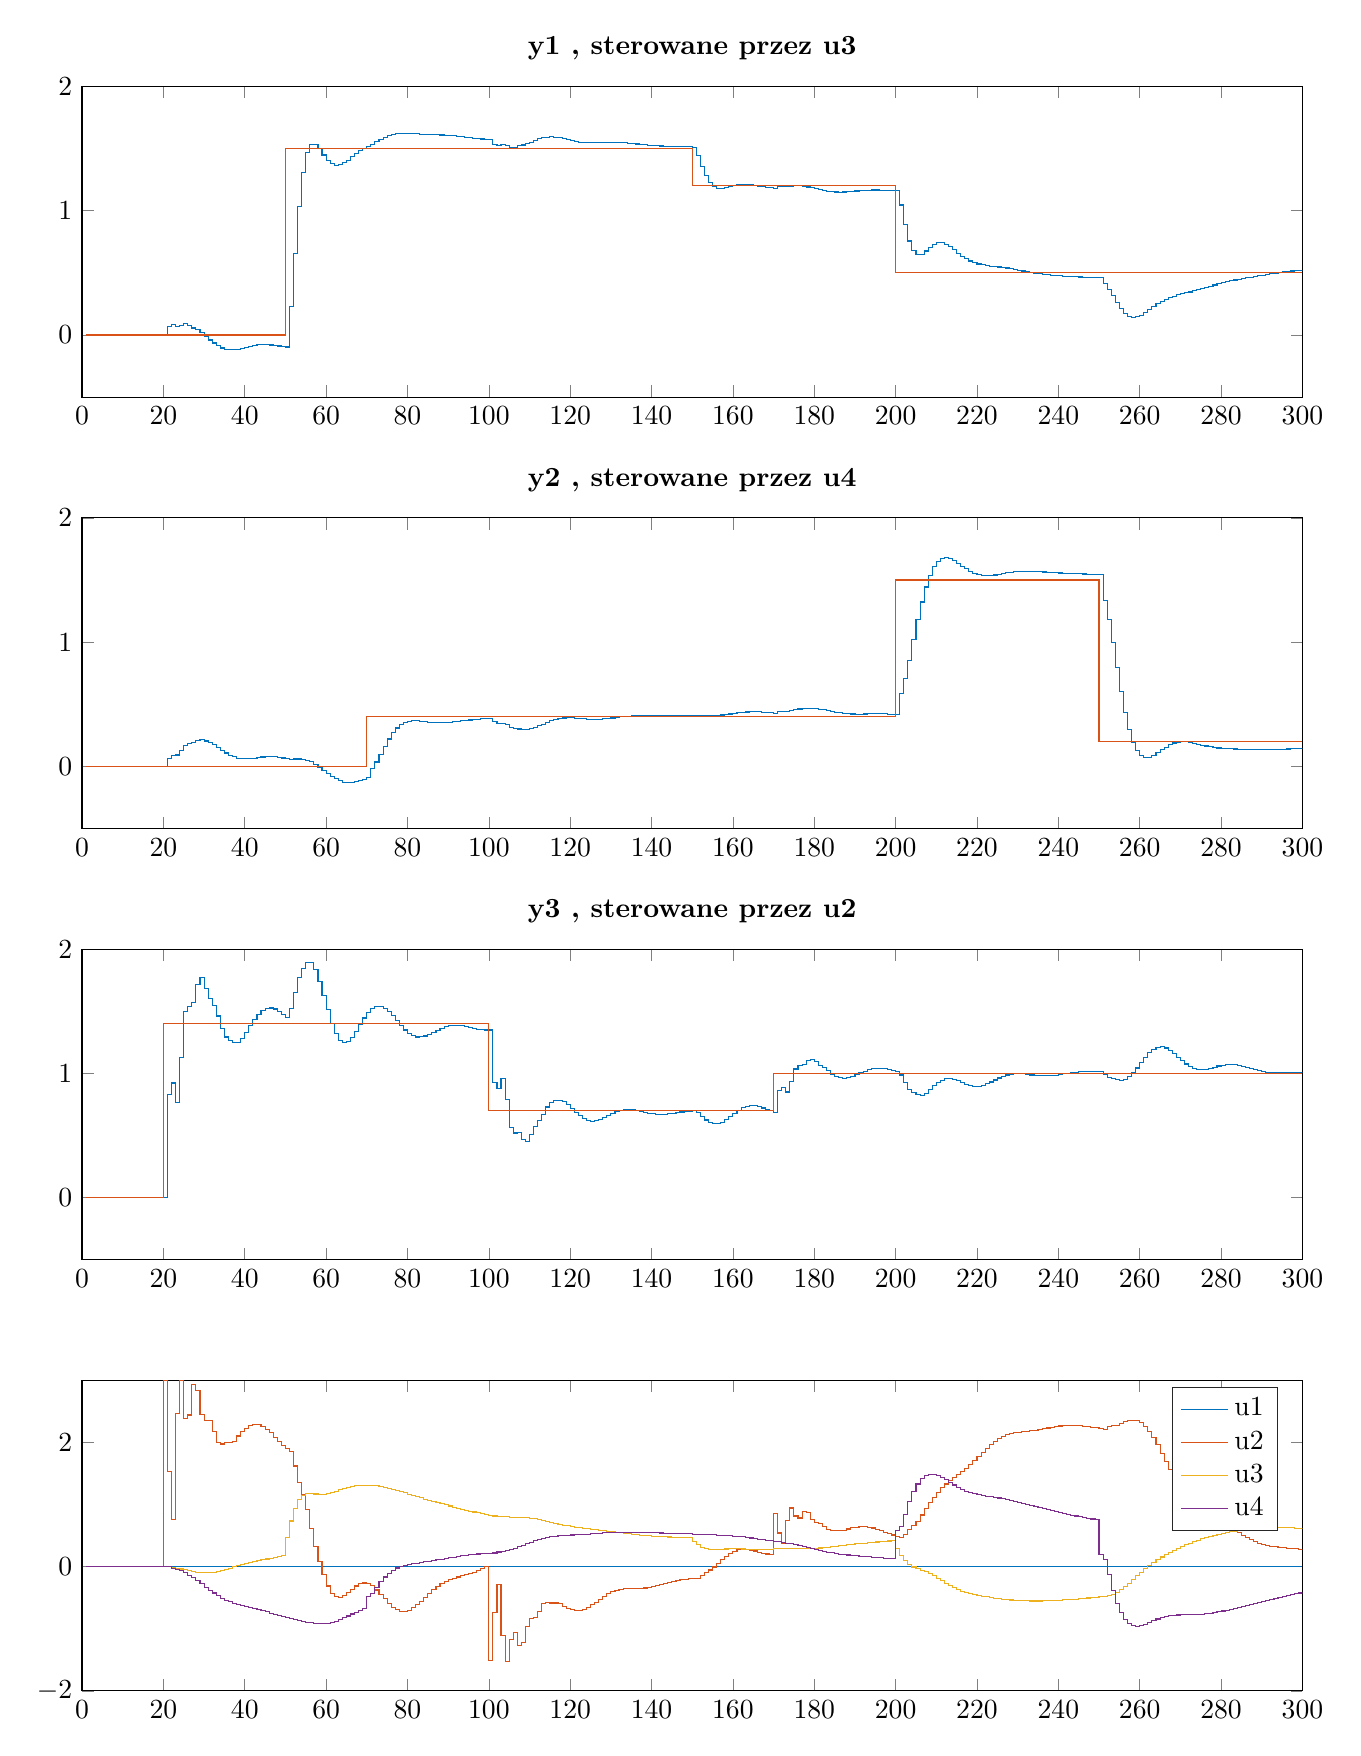
\begin{tikzpicture}

\begin{axis}[%
width=6.102in,
height=1.553in,
at={(1.024in,7.552in)},
scale only axis,
xmin=0,
xmax=300,
ymin=-0.5,
ymax=2,
axis background/.style={fill=white},
title style={font=\bfseries},
title={y1 , sterowane przez u3}
]
\addplot[const plot, color=mycolor1, forget plot] table[row sep=crcr] {%
1	0\\
2	0\\
3	0\\
4	0\\
5	0\\
6	0\\
7	0\\
8	0\\
9	0\\
10	0\\
11	0\\
12	0\\
13	0\\
14	0\\
15	0\\
16	0\\
17	0\\
18	0\\
19	0\\
20	0\\
21	0.0663597650785785\\
22	0.0855245171977065\\
23	0.0667135279482118\\
24	0.0767537132316681\\
25	0.09098543046959\\
26	0.0780193189803143\\
27	0.055934843154834\\
28	0.0405618099629236\\
29	0.020390378759611\\
30	-0.0101133149591592\\
31	-0.0403612142525228\\
32	-0.0646884786946457\\
33	-0.0861839605872635\\
34	-0.10457062698246\\
35	-0.115916537859106\\
36	-0.119912875629224\\
37	-0.119145213808554\\
38	-0.114801561267592\\
39	-0.107335532557434\\
40	-0.0985066079793291\\
41	-0.0903705564115455\\
42	-0.0838988563710679\\
43	-0.0794946559083935\\
44	-0.0775898493726611\\
45	-0.0782396175634967\\
46	-0.0808903801137242\\
47	-0.0847798690436599\\
48	-0.0892023178069689\\
49	-0.0934390345243815\\
50	-0.0967964231354222\\
51	0.231492745388025\\
52	0.652843512281983\\
53	1.03210212380486\\
54	1.30745419447074\\
55	1.46959586482389\\
56	1.5359356193809\\
57	1.53490224471853\\
58	1.4973222906316\\
59	1.44886731560719\\
60	1.40604218454223\\
61	1.3772839210263\\
62	1.36544255460019\\
63	1.36926819062849\\
64	1.38491297308264\\
65	1.40779747334156\\
66	1.43377943911926\\
67	1.45944919422822\\
68	1.48227152777176\\
69	1.50074695171907\\
70	1.51432209850384\\
71	1.53651226687954\\
72	1.55529901425879\\
73	1.57249584200603\\
74	1.58850921388234\\
75	1.60200732293929\\
76	1.61200655536995\\
77	1.61839110308228\\
78	1.62165450120395\\
79	1.62249340834753\\
80	1.62166990814959\\
81	1.61997365315251\\
82	1.61805426110493\\
83	1.61628594736446\\
84	1.61480065268959\\
85	1.61356929799905\\
86	1.61244211609124\\
87	1.61119984757608\\
88	1.60963384205282\\
89	1.60760170283931\\
90	1.60504151323695\\
91	1.60197243338202\\
92	1.59848944369653\\
93	1.59474134555056\\
94	1.59089772307143\\
95	1.58712002930411\\
96	1.58354030896292\\
97	1.58024510168074\\
98	1.57726703868811\\
99	1.57458683709585\\
100	1.57214311039271\\
101	1.53570401533597\\
102	1.52311975760065\\
103	1.5304610397893\\
104	1.52357152079878\\
105	1.51047684522113\\
106	1.51178763941506\\
107	1.52156148396984\\
108	1.52891900834588\\
109	1.53786276354161\\
110	1.5524136266318\\
111	1.56733565826964\\
112	1.57834521433561\\
113	1.58663067083323\\
114	1.59270566960426\\
115	1.59476228091154\\
116	1.592500276701\\
117	1.58753626913275\\
118	1.58096949576288\\
119	1.57322553015918\\
120	1.56524374051907\\
121	1.55819396761915\\
122	1.55264323846042\\
123	1.54870534745017\\
124	1.5464544483224\\
125	1.54580082653643\\
126	1.54633420886035\\
127	1.54751947044078\\
128	1.54888503345522\\
129	1.5500076496664\\
130	1.55051098253221\\
131	1.55015332156506\\
132	1.54886292325782\\
133	1.5466940502779\\
134	1.54379261103009\\
135	1.54038284194934\\
136	1.53673107237309\\
137	1.53309500310216\\
138	1.52969175487602\\
139	1.52668273022869\\
140	1.52416094216785\\
141	1.52214575351909\\
142	1.52059220189146\\
143	1.51940852608683\\
144	1.51847444970839\\
145	1.51766004027854\\
146	1.51684466583872\\
147	1.51593201732462\\
148	1.51485884934844\\
149	1.51359825741546\\
150	1.51215829816161\\
151	1.44451955032585\\
152	1.35850011489635\\
153	1.28120212277366\\
154	1.22502607071249\\
155	1.19182938099536\\
156	1.17809224331223\\
157	1.17806957116615\\
158	1.18552520943478\\
159	1.19525063386874\\
160	1.20387755856867\\
161	1.20966663753889\\
162	1.21201482946333\\
163	1.21115845702117\\
164	1.20787174842879\\
165	1.20309023617026\\
166	1.19767165567242\\
167	1.19233115910687\\
168	1.18760788103586\\
169	1.1838284105481\\
170	1.18112158147365\\
171	1.19410274495222\\
172	1.19781192495238\\
173	1.19369006341906\\
174	1.19610058313876\\
175	1.20134014037814\\
176	1.20035093978277\\
177	1.19551091103096\\
178	1.19138131111893\\
179	1.18621580344052\\
180	1.17832251908483\\
181	1.17002473602939\\
182	1.16326881095307\\
183	1.15766888335804\\
184	1.15312314493608\\
185	1.15050492383504\\
186	1.15001186017445\\
187	1.15098580855726\\
188	1.15295610899263\\
189	1.15571106631327\\
190	1.15879680842953\\
191	1.16164809780842\\
192	1.16395505137743\\
193	1.16560769334859\\
194	1.16652541788344\\
195	1.16671435551384\\
196	1.16633592518864\\
197	1.16562187604396\\
198	1.1647904573977\\
199	1.16404851796901\\
200	1.16358713065022\\
201	1.04622883710174\\
202	0.888750544535498\\
203	0.756596426812266\\
204	0.676534613279114\\
205	0.645975596924462\\
206	0.651111455401245\\
207	0.675925808735911\\
208	0.705704654077842\\
209	0.729533617452949\\
210	0.741750996536476\\
211	0.741204691860816\\
212	0.729458667284753\\
213	0.709514592311172\\
214	0.684978113213299\\
215	0.659214113335385\\
216	0.634764372110395\\
217	0.613258238501604\\
218	0.595533743668817\\
219	0.581740987816264\\
220	0.571495554834857\\
221	0.564106413675138\\
222	0.558767440516869\\
223	0.554671536599526\\
224	0.551097322672091\\
225	0.547480901708567\\
226	0.543445710243924\\
227	0.538794641427489\\
228	0.533489602097854\\
229	0.527623605178898\\
230	0.521380715543781\\
231	0.514991394724043\\
232	0.508693893482005\\
233	0.502703422164027\\
234	0.497188327546194\\
235	0.49225590661925\\
236	0.487949349898966\\
237	0.484253445784068\\
238	0.481106121671905\\
239	0.478414000261803\\
240	0.47606971158795\\
241	0.473968083392996\\
242	0.472019148389935\\
243	0.470157038265954\\
244	0.468344322786598\\
245	0.466571794853057\\
246	0.464854424176912\\
247	0.463224696006995\\
248	0.461724616619293\\
249	0.46039759664978\\
250	0.459281315295422\\
251	0.414885828688705\\
252	0.368257132629104\\
253	0.316594153758868\\
254	0.262192853504933\\
255	0.212934288459213\\
256	0.175133520900087\\
257	0.151624975555428\\
258	0.142420049588145\\
259	0.145952372734542\\
260	0.159602234016325\\
261	0.179984152002327\\
262	0.203689836357104\\
263	0.227957116937345\\
264	0.250801771392311\\
265	0.270957531581761\\
266	0.287888731131994\\
267	0.301706957232726\\
268	0.312932368432814\\
269	0.322273244912892\\
270	0.330492373808294\\
271	0.338291107095995\\
272	0.346203852459195\\
273	0.354553487772744\\
274	0.363463570714449\\
275	0.372888327563601\\
276	0.382652396928249\\
277	0.392506586302617\\
278	0.402186586008989\\
279	0.411458053549282\\
280	0.420146700614253\\
281	0.428156361247082\\
282	0.435472883642325\\
283	0.442153563978706\\
284	0.448307497148181\\
285	0.454072293394227\\
286	0.459590090591437\\
287	0.464985817219951\\
288	0.47035105447292\\
289	0.475735171161519\\
290	0.481143524103869\\
291	0.486541891007557\\
292	0.491865906345174\\
293	0.497033549930411\\
294	0.501958440527685\\
295	0.506562044122575\\
296	0.510783391820091\\
297	0.514585333082359\\
298	0.517956911934208\\
299	0.520912082172043\\
300	0.523485440548571\\
};
\addplot[const plot, color=mycolor2, forget plot] table[row sep=crcr] {%
1	0\\
2	0\\
3	0\\
4	0\\
5	0\\
6	0\\
7	0\\
8	0\\
9	0\\
10	0\\
11	0\\
12	0\\
13	0\\
14	0\\
15	0\\
16	0\\
17	0\\
18	0\\
19	0\\
20	0\\
21	0\\
22	0\\
23	0\\
24	0\\
25	0\\
26	0\\
27	0\\
28	0\\
29	0\\
30	0\\
31	0\\
32	0\\
33	0\\
34	0\\
35	0\\
36	0\\
37	0\\
38	0\\
39	0\\
40	0\\
41	0\\
42	0\\
43	0\\
44	0\\
45	0\\
46	0\\
47	0\\
48	0\\
49	0\\
50	1.5\\
51	1.5\\
52	1.5\\
53	1.5\\
54	1.5\\
55	1.5\\
56	1.5\\
57	1.5\\
58	1.5\\
59	1.5\\
60	1.5\\
61	1.5\\
62	1.5\\
63	1.5\\
64	1.5\\
65	1.5\\
66	1.5\\
67	1.5\\
68	1.5\\
69	1.5\\
70	1.5\\
71	1.5\\
72	1.5\\
73	1.5\\
74	1.5\\
75	1.5\\
76	1.5\\
77	1.5\\
78	1.5\\
79	1.5\\
80	1.5\\
81	1.5\\
82	1.5\\
83	1.5\\
84	1.5\\
85	1.5\\
86	1.5\\
87	1.5\\
88	1.5\\
89	1.5\\
90	1.5\\
91	1.5\\
92	1.5\\
93	1.5\\
94	1.5\\
95	1.5\\
96	1.5\\
97	1.5\\
98	1.5\\
99	1.5\\
100	1.5\\
101	1.5\\
102	1.5\\
103	1.5\\
104	1.5\\
105	1.5\\
106	1.5\\
107	1.5\\
108	1.5\\
109	1.5\\
110	1.5\\
111	1.5\\
112	1.5\\
113	1.5\\
114	1.5\\
115	1.5\\
116	1.5\\
117	1.5\\
118	1.5\\
119	1.5\\
120	1.5\\
121	1.5\\
122	1.5\\
123	1.5\\
124	1.5\\
125	1.5\\
126	1.5\\
127	1.5\\
128	1.5\\
129	1.5\\
130	1.5\\
131	1.5\\
132	1.5\\
133	1.5\\
134	1.5\\
135	1.5\\
136	1.5\\
137	1.5\\
138	1.5\\
139	1.5\\
140	1.5\\
141	1.5\\
142	1.5\\
143	1.5\\
144	1.5\\
145	1.5\\
146	1.5\\
147	1.5\\
148	1.5\\
149	1.5\\
150	1.2\\
151	1.2\\
152	1.2\\
153	1.2\\
154	1.2\\
155	1.2\\
156	1.2\\
157	1.2\\
158	1.2\\
159	1.2\\
160	1.2\\
161	1.2\\
162	1.2\\
163	1.2\\
164	1.2\\
165	1.2\\
166	1.2\\
167	1.2\\
168	1.2\\
169	1.2\\
170	1.2\\
171	1.2\\
172	1.2\\
173	1.2\\
174	1.2\\
175	1.2\\
176	1.2\\
177	1.2\\
178	1.2\\
179	1.2\\
180	1.2\\
181	1.2\\
182	1.2\\
183	1.2\\
184	1.2\\
185	1.2\\
186	1.2\\
187	1.2\\
188	1.2\\
189	1.2\\
190	1.2\\
191	1.2\\
192	1.2\\
193	1.2\\
194	1.2\\
195	1.2\\
196	1.2\\
197	1.2\\
198	1.2\\
199	1.2\\
200	0.5\\
201	0.5\\
202	0.5\\
203	0.5\\
204	0.5\\
205	0.5\\
206	0.5\\
207	0.5\\
208	0.5\\
209	0.5\\
210	0.5\\
211	0.5\\
212	0.5\\
213	0.5\\
214	0.5\\
215	0.5\\
216	0.5\\
217	0.5\\
218	0.5\\
219	0.5\\
220	0.5\\
221	0.5\\
222	0.5\\
223	0.5\\
224	0.5\\
225	0.5\\
226	0.5\\
227	0.5\\
228	0.5\\
229	0.5\\
230	0.5\\
231	0.5\\
232	0.5\\
233	0.5\\
234	0.5\\
235	0.5\\
236	0.5\\
237	0.5\\
238	0.5\\
239	0.5\\
240	0.5\\
241	0.5\\
242	0.5\\
243	0.5\\
244	0.5\\
245	0.5\\
246	0.5\\
247	0.5\\
248	0.5\\
249	0.5\\
250	0.5\\
251	0.5\\
252	0.5\\
253	0.5\\
254	0.5\\
255	0.5\\
256	0.5\\
257	0.5\\
258	0.5\\
259	0.5\\
260	0.5\\
261	0.5\\
262	0.5\\
263	0.5\\
264	0.5\\
265	0.5\\
266	0.5\\
267	0.5\\
268	0.5\\
269	0.5\\
270	0.5\\
271	0.5\\
272	0.5\\
273	0.5\\
274	0.5\\
275	0.5\\
276	0.5\\
277	0.5\\
278	0.5\\
279	0.5\\
280	0.5\\
281	0.5\\
282	0.5\\
283	0.5\\
284	0.5\\
285	0.5\\
286	0.5\\
287	0.5\\
288	0.5\\
289	0.5\\
290	0.5\\
291	0.5\\
292	0.5\\
293	0.5\\
294	0.5\\
295	0.5\\
296	0.5\\
297	0.5\\
298	0.5\\
299	0.5\\
300	0.5\\
};
\end{axis}

\begin{axis}[%
width=6.102in,
height=1.553in,
at={(1.024in,5.395in)},
scale only axis,
xmin=0,
xmax=300,
ymin=-0.5,
ymax=2,
axis background/.style={fill=white},
title style={font=\bfseries},
title={y2 , sterowane przez u4}
]
\addplot[const plot, color=mycolor1, forget plot] table[row sep=crcr] {%
1	0\\
2	0\\
3	0\\
4	0\\
5	0\\
6	0\\
7	0\\
8	0\\
9	0\\
10	0\\
11	0\\
12	0\\
13	0\\
14	0\\
15	0\\
16	0\\
17	0\\
18	0\\
19	0\\
20	0\\
21	0.0612158143362928\\
22	0.0899376290312318\\
23	0.0917787502603558\\
24	0.1257994021792\\
25	0.16674635201832\\
26	0.184152979184844\\
27	0.193883706875663\\
28	0.208016101426467\\
29	0.21362729115698\\
30	0.204568114302619\\
31	0.189694415722039\\
32	0.173340216464586\\
33	0.152712235248173\\
34	0.129114369465564\\
35	0.107594647250844\\
36	0.0900506171811917\\
37	0.0759396370591599\\
38	0.0659471498634879\\
39	0.0610162433677259\\
40	0.0603785835536465\\
41	0.0625132662627267\\
42	0.0664008563149663\\
43	0.0710871894319955\\
44	0.0752903827465415\\
45	0.0779491857080521\\
46	0.0785692256200994\\
47	0.0769740015926108\\
48	0.0731682146419604\\
49	0.0674592876158287\\
50	0.0604237377230922\\
51	0.0579397047779779\\
52	0.0596392449541273\\
53	0.0595803279720908\\
54	0.0554309148760159\\
55	0.0477974727000989\\
56	0.0356036105699228\\
57	0.0175576609929984\\
58	-0.00516597688082949\\
59	-0.0302238723984627\\
60	-0.0558221810770392\\
61	-0.0802093789395458\\
62	-0.101248947902934\\
63	-0.117236968210479\\
64	-0.127418704769508\\
65	-0.131681086097274\\
66	-0.130365716821451\\
67	-0.124394583760381\\
68	-0.11516379113673\\
69	-0.104202131489666\\
70	-0.0929567694960565\\
71	-0.0191628459790696\\
72	0.0351206319221365\\
73	0.0956871998322585\\
74	0.160495579077754\\
75	0.219911504090896\\
76	0.269717970998332\\
77	0.308614412184295\\
78	0.336578836539787\\
79	0.354542578521814\\
80	0.364139888928646\\
81	0.36742424973261\\
82	0.366505425352904\\
83	0.363256688895838\\
84	0.359203630809598\\
85	0.355488774317992\\
86	0.352841138110021\\
87	0.351601196430849\\
88	0.35181058359079\\
89	0.353308236713116\\
90	0.355808674470177\\
91	0.358977206505164\\
92	0.362497807957608\\
93	0.366115248077269\\
94	0.369651814393026\\
95	0.373009950831969\\
96	0.376163787140078\\
97	0.379139690076471\\
98	0.381992200747052\\
99	0.384782377942177\\
100	0.387560681692625\\
101	0.358859403067462\\
102	0.346457023243965\\
103	0.348201788646485\\
104	0.333981076786958\\
105	0.312583922744137\\
106	0.303217590581807\\
107	0.300657698736013\\
108	0.296386181217003\\
109	0.295738644802912\\
110	0.303296428163692\\
111	0.314790338285078\\
112	0.326715408876741\\
113	0.340049744093242\\
114	0.354504642180694\\
115	0.367384034856125\\
116	0.377320646241285\\
117	0.384666734248394\\
118	0.389393567710021\\
119	0.391151567674141\\
120	0.390421977871405\\
121	0.388215704548203\\
122	0.385280533167699\\
123	0.382196728050147\\
124	0.379656105733669\\
125	0.37823324358276\\
126	0.37815732505244\\
127	0.379427866499327\\
128	0.381935837572851\\
129	0.385426569739593\\
130	0.389509619719677\\
131	0.393771021574015\\
132	0.397848189951582\\
133	0.401440489194288\\
134	0.404330422852791\\
135	0.406416066004548\\
136	0.407709531237662\\
137	0.4083086610112\\
138	0.408371994068193\\
139	0.408095674056377\\
140	0.407682384949553\\
141	0.407311345998716\\
142	0.407119842224738\\
143	0.407193862363311\\
144	0.407564171548503\\
145	0.408209778785561\\
146	0.409069052107364\\
147	0.410054417255571\\
148	0.411067391961154\\
149	0.412012960565216\\
150	0.412811895978435\\
151	0.412362334057975\\
152	0.410831896098505\\
153	0.409520025166228\\
154	0.409005802849071\\
155	0.409261816724132\\
156	0.410570132667945\\
157	0.41322826431546\\
158	0.417011566792463\\
159	0.421433852538412\\
160	0.426098356513704\\
161	0.430605490489242\\
162	0.434475064655151\\
163	0.437316780914397\\
164	0.438940007106923\\
165	0.439296426412256\\
166	0.438443852374353\\
167	0.436570565501127\\
168	0.433971806088162\\
169	0.430977883261949\\
170	0.42790696430876\\
171	0.438541956767048\\
172	0.442628769869444\\
173	0.441211327083458\\
174	0.447215781356679\\
175	0.456811914302337\\
176	0.461639705706879\\
177	0.463768415892375\\
178	0.466666537192888\\
179	0.467879973358441\\
180	0.465311770509479\\
181	0.460704049346472\\
182	0.455523115339533\\
183	0.449363772828795\\
184	0.442404816616721\\
185	0.435885232779499\\
186	0.430488888811946\\
187	0.426162974712825\\
188	0.423005886531954\\
189	0.421232521025342\\
190	0.420675834586646\\
191	0.420914967966071\\
192	0.421617577393276\\
193	0.422504210241811\\
194	0.423235714479816\\
195	0.423518773647064\\
196	0.423210632664778\\
197	0.422275123198753\\
198	0.420734504989662\\
199	0.418687012376997\\
200	0.416302279675471\\
201	0.586078292456875\\
202	0.705697068936199\\
203	0.850847329703701\\
204	1.01773739908994\\
205	1.17920482888817\\
206	1.32284403402213\\
207	1.44371574637569\\
208	1.53894274364366\\
209	1.60776217696648\\
210	1.65190708420773\\
211	1.6747831549607\\
212	1.68038623325741\\
213	1.67289737567105\\
214	1.65654764888656\\
215	1.63524797543925\\
216	1.61225597637403\\
217	1.59012827353306\\
218	1.57075378373407\\
219	1.55532841621152\\
220	1.54438483049827\\
221	1.53792162311566\\
222	1.53553862152413\\
223	1.5365433263071\\
224	1.54006768275445\\
225	1.54519359020797\\
226	1.55105064494783\\
227	1.55688108818473\\
228	1.56208706360677\\
229	1.56625846784464\\
230	1.56917384561703\\
231	1.57078049204266\\
232	1.57116408334223\\
233	1.57051127927035\\
234	1.56906780276233\\
235	1.56709828109609\\
236	1.56485307947925\\
237	1.56254358320928\\
238	1.56032640888849\\
239	1.55829719740518\\
240	1.55649321016524\\
241	1.55490240978034\\
242	1.5534765936052\\
243	1.55214646230776\\
244	1.55083646804822\\
245	1.54947750253923\\
246	1.54801621376195\\
247	1.54642045931575\\
248	1.54468088623705\\
249	1.54280907377556\\
250	1.5408330927514\\
251	1.33226931982931\\
252	1.18064608039916\\
253	1.0003185469293\\
254	0.797472397195155\\
255	0.6041203333921\\
256	0.435585875231599\\
257	0.298343292300837\\
258	0.194955152368881\\
259	0.124759033280372\\
260	0.0844139860558817\\
261	0.0686424072231572\\
262	0.0713065096899602\\
263	0.0863588041886838\\
264	0.108299451517581\\
265	0.132444013406579\\
266	0.155200977498579\\
267	0.174177554596581\\
268	0.188059439441514\\
269	0.196429350469059\\
270	0.19959260227103\\
271	0.198361835012168\\
272	0.193817994306914\\
273	0.187114985519491\\
274	0.179340635707133\\
275	0.171412748897079\\
276	0.16401396611159\\
277	0.157576005774502\\
278	0.152301013119626\\
279	0.148201523976391\\
280	0.145151968522589\\
281	0.142946531423089\\
282	0.141352950535608\\
283	0.140154386407934\\
284	0.139177982103772\\
285	0.138310426320914\\
286	0.137500555919916\\
287	0.136751115460893\\
288	0.136103819785571\\
289	0.135621547096211\\
290	0.135370553727059\\
291	0.135405311780554\\
292	0.135757988033001\\
293	0.136433344881853\\
294	0.137408789349994\\
295	0.138638743489113\\
296	0.140062092501357\\
297	0.141611139161449\\
298	0.143220498562903\\
299	0.144834668629122\\
300	0.146413393539237\\
};
\addplot[const plot, color=mycolor2, forget plot] table[row sep=crcr] {%
1	0\\
2	0\\
3	0\\
4	0\\
5	0\\
6	0\\
7	0\\
8	0\\
9	0\\
10	0\\
11	0\\
12	0\\
13	0\\
14	0\\
15	0\\
16	0\\
17	0\\
18	0\\
19	0\\
20	0\\
21	0\\
22	0\\
23	0\\
24	0\\
25	0\\
26	0\\
27	0\\
28	0\\
29	0\\
30	0\\
31	0\\
32	0\\
33	0\\
34	0\\
35	0\\
36	0\\
37	0\\
38	0\\
39	0\\
40	0\\
41	0\\
42	0\\
43	0\\
44	0\\
45	0\\
46	0\\
47	0\\
48	0\\
49	0\\
50	0\\
51	0\\
52	0\\
53	0\\
54	0\\
55	0\\
56	0\\
57	0\\
58	0\\
59	0\\
60	0\\
61	0\\
62	0\\
63	0\\
64	0\\
65	0\\
66	0\\
67	0\\
68	0\\
69	0\\
70	0.4\\
71	0.4\\
72	0.4\\
73	0.4\\
74	0.4\\
75	0.4\\
76	0.4\\
77	0.4\\
78	0.4\\
79	0.4\\
80	0.4\\
81	0.4\\
82	0.4\\
83	0.4\\
84	0.4\\
85	0.4\\
86	0.4\\
87	0.4\\
88	0.4\\
89	0.4\\
90	0.4\\
91	0.4\\
92	0.4\\
93	0.4\\
94	0.4\\
95	0.4\\
96	0.4\\
97	0.4\\
98	0.4\\
99	0.4\\
100	0.4\\
101	0.4\\
102	0.4\\
103	0.4\\
104	0.4\\
105	0.4\\
106	0.4\\
107	0.4\\
108	0.4\\
109	0.4\\
110	0.4\\
111	0.4\\
112	0.4\\
113	0.4\\
114	0.4\\
115	0.4\\
116	0.4\\
117	0.4\\
118	0.4\\
119	0.4\\
120	0.4\\
121	0.4\\
122	0.4\\
123	0.4\\
124	0.4\\
125	0.4\\
126	0.4\\
127	0.4\\
128	0.4\\
129	0.4\\
130	0.4\\
131	0.4\\
132	0.4\\
133	0.4\\
134	0.4\\
135	0.4\\
136	0.4\\
137	0.4\\
138	0.4\\
139	0.4\\
140	0.4\\
141	0.4\\
142	0.4\\
143	0.4\\
144	0.4\\
145	0.4\\
146	0.4\\
147	0.4\\
148	0.4\\
149	0.4\\
150	0.4\\
151	0.4\\
152	0.4\\
153	0.4\\
154	0.4\\
155	0.4\\
156	0.4\\
157	0.4\\
158	0.4\\
159	0.4\\
160	0.4\\
161	0.4\\
162	0.4\\
163	0.4\\
164	0.4\\
165	0.4\\
166	0.4\\
167	0.4\\
168	0.4\\
169	0.4\\
170	0.4\\
171	0.4\\
172	0.4\\
173	0.4\\
174	0.4\\
175	0.4\\
176	0.4\\
177	0.4\\
178	0.4\\
179	0.4\\
180	0.4\\
181	0.4\\
182	0.4\\
183	0.4\\
184	0.4\\
185	0.4\\
186	0.4\\
187	0.4\\
188	0.4\\
189	0.4\\
190	0.4\\
191	0.4\\
192	0.4\\
193	0.4\\
194	0.4\\
195	0.4\\
196	0.4\\
197	0.4\\
198	0.4\\
199	0.4\\
200	1.5\\
201	1.5\\
202	1.5\\
203	1.5\\
204	1.5\\
205	1.5\\
206	1.5\\
207	1.5\\
208	1.5\\
209	1.5\\
210	1.5\\
211	1.5\\
212	1.5\\
213	1.5\\
214	1.5\\
215	1.5\\
216	1.5\\
217	1.5\\
218	1.5\\
219	1.5\\
220	1.5\\
221	1.5\\
222	1.5\\
223	1.5\\
224	1.5\\
225	1.5\\
226	1.5\\
227	1.5\\
228	1.5\\
229	1.5\\
230	1.5\\
231	1.5\\
232	1.5\\
233	1.5\\
234	1.5\\
235	1.5\\
236	1.5\\
237	1.5\\
238	1.5\\
239	1.5\\
240	1.5\\
241	1.5\\
242	1.5\\
243	1.5\\
244	1.5\\
245	1.5\\
246	1.5\\
247	1.5\\
248	1.5\\
249	1.5\\
250	0.2\\
251	0.2\\
252	0.2\\
253	0.2\\
254	0.2\\
255	0.2\\
256	0.2\\
257	0.2\\
258	0.2\\
259	0.2\\
260	0.2\\
261	0.2\\
262	0.2\\
263	0.2\\
264	0.2\\
265	0.2\\
266	0.2\\
267	0.2\\
268	0.2\\
269	0.2\\
270	0.2\\
271	0.2\\
272	0.2\\
273	0.2\\
274	0.2\\
275	0.2\\
276	0.2\\
277	0.2\\
278	0.2\\
279	0.2\\
280	0.2\\
281	0.2\\
282	0.2\\
283	0.2\\
284	0.2\\
285	0.2\\
286	0.2\\
287	0.2\\
288	0.2\\
289	0.2\\
290	0.2\\
291	0.2\\
292	0.2\\
293	0.2\\
294	0.2\\
295	0.2\\
296	0.2\\
297	0.2\\
298	0.2\\
299	0.2\\
300	0.2\\
};
\end{axis}

\begin{axis}[%
width=6.102in,
height=1.553in,
at={(1.024in,3.239in)},
scale only axis,
xmin=0,
xmax=300,
ymin=-0.5,
ymax=2,
axis background/.style={fill=white},
title style={font=\bfseries},
title={y3 , sterowane przez u2}
]
\addplot[const plot, color=mycolor1, forget plot] table[row sep=crcr] {%
1	0\\
2	0\\
3	0\\
4	0\\
5	0\\
6	0\\
7	0\\
8	0\\
9	0\\
10	0\\
11	0\\
12	0\\
13	0\\
14	0\\
15	0\\
16	0\\
17	0\\
18	0\\
19	0\\
20	0\\
21	0.82628561460347\\
22	0.922573222384271\\
23	0.763319694086904\\
24	1.13005547952617\\
25	1.49433160730769\\
26	1.53725530475204\\
27	1.57013442380353\\
28	1.71582637540012\\
29	1.76850290001018\\
30	1.6849014892166\\
31	1.60208763738997\\
32	1.54752646035891\\
33	1.46149650522228\\
34	1.3587797488548\\
35	1.29245519567932\\
36	1.26254341258647\\
37	1.24718289156284\\
38	1.25143303450171\\
39	1.28375742700331\\
40	1.3320054641446\\
41	1.3817620602522\\
42	1.42981337782161\\
43	1.47354145588669\\
44	1.50582306231409\\
45	1.52272291464025\\
46	1.52588300227942\\
47	1.51766996601916\\
48	1.49989244751017\\
49	1.47598364259355\\
50	1.45054058197622\\
51	1.51842982377051\\
52	1.65354172292851\\
53	1.76818528060611\\
54	1.8430959471454\\
55	1.89091656335852\\
56	1.89433682934659\\
57	1.83846265387386\\
58	1.74166349879895\\
59	1.62907169852763\\
60	1.51271523220212\\
61	1.40392297048415\\
62	1.31865920383723\\
63	1.26639967606219\\
64	1.24672061103168\\
65	1.25594532438455\\
66	1.28928664204355\\
67	1.33857506345927\\
68	1.39359018249314\\
69	1.44555465418713\\
70	1.48800416118909\\
71	1.52276137796753\\
72	1.54065323621122\\
73	1.53940990878228\\
74	1.52453197760378\\
75	1.49883748577952\\
76	1.46352295977279\\
77	1.42324669447462\\
78	1.38390821090577\\
79	1.34909684346458\\
80	1.3210370908276\\
81	1.30192165788574\\
82	1.29283675534477\\
83	1.29303136767858\\
84	1.30078955477543\\
85	1.31410733262107\\
86	1.33060130198469\\
87	1.34768438785201\\
88	1.36313448161615\\
89	1.37537534885198\\
90	1.38343579657032\\
91	1.38696199158602\\
92	1.38625473567408\\
93	1.38213684579434\\
94	1.37572496705794\\
95	1.3682515231585\\
96	1.3609195254956\\
97	1.35474797862447\\
98	1.35045459902286\\
99	1.34841450693192\\
100	1.34867062986483\\
101	0.92584853140612\\
102	0.874312162829712\\
103	0.961727488479733\\
104	0.786409418426808\\
105	0.562040353785915\\
106	0.519412740393368\\
107	0.524043494142734\\
108	0.469264944859732\\
109	0.448480144623612\\
110	0.506761623947168\\
111	0.573787997462869\\
112	0.618306301350896\\
113	0.669953886074735\\
114	0.729123540556388\\
115	0.767249005574206\\
116	0.780071394182586\\
117	0.781253162825343\\
118	0.772149415059826\\
119	0.748628004209799\\
120	0.716733606606186\\
121	0.685618962059392\\
122	0.65820616460772\\
123	0.635461800372987\\
124	0.620548477400482\\
125	0.615422731333741\\
126	0.618774241561793\\
127	0.628462761997338\\
128	0.642835841756361\\
129	0.65971370032285\\
130	0.676355787217372\\
131	0.690613985786267\\
132	0.701260087073321\\
133	0.707577648003388\\
134	0.709355893906118\\
135	0.707098331834996\\
136	0.701837215798492\\
137	0.694778872876522\\
138	0.687151195461313\\
139	0.680122556582256\\
140	0.674632950701179\\
141	0.671261976952043\\
142	0.670226448502169\\
143	0.671426880442458\\
144	0.674490668063948\\
145	0.678847926180131\\
146	0.683843078236686\\
147	0.688836686889591\\
148	0.693278880919759\\
149	0.696764923514421\\
150	0.699070351861913\\
151	0.681905684569529\\
152	0.651086157030225\\
153	0.624747796859649\\
154	0.607244206231071\\
155	0.596311017312742\\
156	0.59546303759112\\
157	0.607592450189619\\
158	0.628810152465891\\
159	0.653766810755139\\
160	0.679698625641693\\
161	0.704010544888543\\
162	0.723237449281774\\
163	0.735289835345218\\
164	0.740156775990029\\
165	0.738577620457043\\
166	0.731594555905243\\
167	0.720983554339466\\
168	0.708964292310219\\
169	0.697474345489412\\
170	0.687969407239893\\
171	0.863711353571909\\
172	0.88461704198701\\
173	0.849941614796221\\
174	0.931019370592158\\
175	1.03519787319166\\
176	1.06238220168099\\
177	1.06905039064412\\
178	1.09995227228068\\
179	1.11439911692976\\
180	1.09274810782869\\
181	1.0651299579825\\
182	1.04521480419321\\
183	1.02078703933007\\
184	0.992275941573381\\
185	0.972539009644601\\
186	0.963955316572527\\
187	0.961100163819071\\
188	0.963660516867336\\
189	0.973501232331597\\
190	0.987966072788157\\
191	1.00293852373607\\
192	1.01688700286843\\
193	1.02908124253546\\
194	1.03785955814398\\
195	1.04212492853847\\
196	1.04225457223985\\
197	1.03906888296089\\
198	1.0332668149002\\
199	1.0258495806965\\
200	1.01811546916358\\
201	0.986503292284717\\
202	0.926407871595017\\
203	0.872597001281577\\
204	0.842577538702166\\
205	0.827297533497073\\
206	0.824652963879624\\
207	0.840195429872236\\
208	0.868800253768874\\
209	0.898852291792988\\
210	0.924798051857236\\
211	0.945211700001832\\
212	0.957164754902112\\
213	0.958703274350533\\
214	0.95176787413019\\
215	0.939837961808069\\
216	0.925661649590044\\
217	0.911919521346917\\
218	0.901534484987715\\
219	0.896515623653882\\
220	0.897452984872348\\
221	0.904063926905918\\
222	0.915491547014137\\
223	0.930230850679827\\
224	0.946377949297387\\
225	0.962108753980101\\
226	0.975923161767638\\
227	0.986708427600033\\
228	0.993844937780214\\
229	0.997277960388234\\
230	0.997438580672833\\
231	0.995092541685551\\
232	0.991206357967571\\
233	0.986811291049662\\
234	0.982853299484268\\
235	0.980074354963484\\
236	0.978950628748667\\
237	0.979672028376871\\
238	0.982153558412463\\
239	0.986082435794841\\
240	0.990992348166204\\
241	0.996345449583031\\
242	1.00160974866983\\
243	1.00632614029436\\
244	1.01015786579659\\
245	1.01291645898112\\
246	1.01456445363921\\
247	1.01519895676253\\
248	1.01502060373354\\
249	1.01429332749793\\
250	1.01330167294657\\
251	0.991107108057327\\
252	0.96989181047104\\
253	0.958601257449013\\
254	0.947998012156859\\
255	0.941433170300771\\
256	0.949666803309577\\
257	0.972680484416846\\
258	1.00453116344368\\
259	1.04317948302616\\
260	1.08692024607966\\
261	1.13005635014258\\
262	1.16664656187859\\
263	1.19368572799002\\
264	1.20950058021572\\
265	1.2127640635793\\
266	1.2038297742411\\
267	1.18504278497927\\
268	1.15951406843121\\
269	1.13045427541652\\
270	1.10121618140358\\
271	1.07492797396216\\
272	1.05387046391072\\
273	1.03929967093731\\
274	1.03157816755208\\
275	1.03023167707929\\
276	1.03403380283646\\
277	1.0412812671836\\
278	1.05011935460814\\
279	1.05877694993367\\
280	1.06575117777139\\
281	1.06997138892104\\
282	1.07088540736876\\
283	1.06844591220206\\
284	1.06303797000403\\
285	1.05537473256823\\
286	1.04636317831856\\
287	1.03695764879047\\
288	1.02803116829403\\
289	1.02027924623282\\
290	1.01415808373843\\
291	1.00986033134481\\
292	1.00732934911871\\
293	1.00630406816786\\
294	1.00638247701177\\
295	1.00709345277027\\
296	1.007967523809\\
297	1.00859722105893\\
298	1.0086802717562\\
299	1.00804289936662\\
300	1.00664338757777\\
};
\addplot[const plot, color=mycolor2, forget plot] table[row sep=crcr] {%
1	0\\
2	0\\
3	0\\
4	0\\
5	0\\
6	0\\
7	0\\
8	0\\
9	0\\
10	0\\
11	0\\
12	0\\
13	0\\
14	0\\
15	0\\
16	0\\
17	0\\
18	0\\
19	0\\
20	1.4\\
21	1.4\\
22	1.4\\
23	1.4\\
24	1.4\\
25	1.4\\
26	1.4\\
27	1.4\\
28	1.4\\
29	1.4\\
30	1.4\\
31	1.4\\
32	1.4\\
33	1.4\\
34	1.4\\
35	1.4\\
36	1.4\\
37	1.4\\
38	1.4\\
39	1.4\\
40	1.4\\
41	1.4\\
42	1.4\\
43	1.4\\
44	1.4\\
45	1.4\\
46	1.4\\
47	1.4\\
48	1.4\\
49	1.4\\
50	1.4\\
51	1.4\\
52	1.4\\
53	1.4\\
54	1.4\\
55	1.4\\
56	1.4\\
57	1.4\\
58	1.4\\
59	1.4\\
60	1.4\\
61	1.4\\
62	1.4\\
63	1.4\\
64	1.4\\
65	1.4\\
66	1.4\\
67	1.4\\
68	1.4\\
69	1.4\\
70	1.4\\
71	1.4\\
72	1.4\\
73	1.4\\
74	1.4\\
75	1.4\\
76	1.4\\
77	1.4\\
78	1.4\\
79	1.4\\
80	1.4\\
81	1.4\\
82	1.4\\
83	1.4\\
84	1.4\\
85	1.4\\
86	1.4\\
87	1.4\\
88	1.4\\
89	1.4\\
90	1.4\\
91	1.4\\
92	1.4\\
93	1.4\\
94	1.4\\
95	1.4\\
96	1.4\\
97	1.4\\
98	1.4\\
99	1.4\\
100	0.7\\
101	0.7\\
102	0.7\\
103	0.7\\
104	0.7\\
105	0.7\\
106	0.7\\
107	0.7\\
108	0.7\\
109	0.7\\
110	0.7\\
111	0.7\\
112	0.7\\
113	0.7\\
114	0.7\\
115	0.7\\
116	0.7\\
117	0.7\\
118	0.7\\
119	0.7\\
120	0.7\\
121	0.7\\
122	0.7\\
123	0.7\\
124	0.7\\
125	0.7\\
126	0.7\\
127	0.7\\
128	0.7\\
129	0.7\\
130	0.7\\
131	0.7\\
132	0.7\\
133	0.7\\
134	0.7\\
135	0.7\\
136	0.7\\
137	0.7\\
138	0.7\\
139	0.7\\
140	0.7\\
141	0.7\\
142	0.7\\
143	0.7\\
144	0.7\\
145	0.7\\
146	0.7\\
147	0.7\\
148	0.7\\
149	0.7\\
150	0.7\\
151	0.7\\
152	0.7\\
153	0.7\\
154	0.7\\
155	0.7\\
156	0.7\\
157	0.7\\
158	0.7\\
159	0.7\\
160	0.7\\
161	0.7\\
162	0.7\\
163	0.7\\
164	0.7\\
165	0.7\\
166	0.7\\
167	0.7\\
168	0.7\\
169	0.7\\
170	1\\
171	1\\
172	1\\
173	1\\
174	1\\
175	1\\
176	1\\
177	1\\
178	1\\
179	1\\
180	1\\
181	1\\
182	1\\
183	1\\
184	1\\
185	1\\
186	1\\
187	1\\
188	1\\
189	1\\
190	1\\
191	1\\
192	1\\
193	1\\
194	1\\
195	1\\
196	1\\
197	1\\
198	1\\
199	1\\
200	1\\
201	1\\
202	1\\
203	1\\
204	1\\
205	1\\
206	1\\
207	1\\
208	1\\
209	1\\
210	1\\
211	1\\
212	1\\
213	1\\
214	1\\
215	1\\
216	1\\
217	1\\
218	1\\
219	1\\
220	1\\
221	1\\
222	1\\
223	1\\
224	1\\
225	1\\
226	1\\
227	1\\
228	1\\
229	1\\
230	1\\
231	1\\
232	1\\
233	1\\
234	1\\
235	1\\
236	1\\
237	1\\
238	1\\
239	1\\
240	1\\
241	1\\
242	1\\
243	1\\
244	1\\
245	1\\
246	1\\
247	1\\
248	1\\
249	1\\
250	1\\
251	1\\
252	1\\
253	1\\
254	1\\
255	1\\
256	1\\
257	1\\
258	1\\
259	1\\
260	1\\
261	1\\
262	1\\
263	1\\
264	1\\
265	1\\
266	1\\
267	1\\
268	1\\
269	1\\
270	1\\
271	1\\
272	1\\
273	1\\
274	1\\
275	1\\
276	1\\
277	1\\
278	1\\
279	1\\
280	1\\
281	1\\
282	1\\
283	1\\
284	1\\
285	1\\
286	1\\
287	1\\
288	1\\
289	1\\
290	1\\
291	1\\
292	1\\
293	1\\
294	1\\
295	1\\
296	1\\
297	1\\
298	1\\
299	1\\
300	1\\
};
\end{axis}

\begin{axis}[%
width=6.102in,
height=1.553in,
at={(1.024in,1.083in)},
scale only axis,
xmin=0,
xmax=300,
ymin=-2,
ymax=3,
axis background/.style={fill=white},
legend style={legend cell align=left, align=left, draw=white!15!black}
]
\addplot[const plot, color=mycolor1] table[row sep=crcr] {%
1	0\\
2	0\\
3	0\\
4	0\\
5	0\\
6	0\\
7	0\\
8	0\\
9	0\\
10	0\\
11	0\\
12	0\\
13	0\\
14	0\\
15	0\\
16	0\\
17	0\\
18	0\\
19	0\\
20	0\\
21	0\\
22	0\\
23	0\\
24	0\\
25	0\\
26	0\\
27	0\\
28	0\\
29	0\\
30	0\\
31	0\\
32	0\\
33	0\\
34	0\\
35	0\\
36	0\\
37	0\\
38	0\\
39	0\\
40	0\\
41	0\\
42	0\\
43	0\\
44	0\\
45	0\\
46	0\\
47	0\\
48	0\\
49	0\\
50	0\\
51	0\\
52	0\\
53	0\\
54	0\\
55	0\\
56	0\\
57	0\\
58	0\\
59	0\\
60	0\\
61	0\\
62	0\\
63	0\\
64	0\\
65	0\\
66	0\\
67	0\\
68	0\\
69	0\\
70	0\\
71	0\\
72	0\\
73	0\\
74	0\\
75	0\\
76	0\\
77	0\\
78	0\\
79	0\\
80	0\\
81	0\\
82	0\\
83	0\\
84	0\\
85	0\\
86	0\\
87	0\\
88	0\\
89	0\\
90	0\\
91	0\\
92	0\\
93	0\\
94	0\\
95	0\\
96	0\\
97	0\\
98	0\\
99	0\\
100	0\\
101	0\\
102	0\\
103	0\\
104	0\\
105	0\\
106	0\\
107	0\\
108	0\\
109	0\\
110	0\\
111	0\\
112	0\\
113	0\\
114	0\\
115	0\\
116	0\\
117	0\\
118	0\\
119	0\\
120	0\\
121	0\\
122	0\\
123	0\\
124	0\\
125	0\\
126	0\\
127	0\\
128	0\\
129	0\\
130	0\\
131	0\\
132	0\\
133	0\\
134	0\\
135	0\\
136	0\\
137	0\\
138	0\\
139	0\\
140	0\\
141	0\\
142	0\\
143	0\\
144	0\\
145	0\\
146	0\\
147	0\\
148	0\\
149	0\\
150	0\\
151	0\\
152	0\\
153	0\\
154	0\\
155	0\\
156	0\\
157	0\\
158	0\\
159	0\\
160	0\\
161	0\\
162	0\\
163	0\\
164	0\\
165	0\\
166	0\\
167	0\\
168	0\\
169	0\\
170	0\\
171	0\\
172	0\\
173	0\\
174	0\\
175	0\\
176	0\\
177	0\\
178	0\\
179	0\\
180	0\\
181	0\\
182	0\\
183	0\\
184	0\\
185	0\\
186	0\\
187	0\\
188	0\\
189	0\\
190	0\\
191	0\\
192	0\\
193	0\\
194	0\\
195	0\\
196	0\\
197	0\\
198	0\\
199	0\\
200	0\\
201	0\\
202	0\\
203	0\\
204	0\\
205	0\\
206	0\\
207	0\\
208	0\\
209	0\\
210	0\\
211	0\\
212	0\\
213	0\\
214	0\\
215	0\\
216	0\\
217	0\\
218	0\\
219	0\\
220	0\\
221	0\\
222	0\\
223	0\\
224	0\\
225	0\\
226	0\\
227	0\\
228	0\\
229	0\\
230	0\\
231	0\\
232	0\\
233	0\\
234	0\\
235	0\\
236	0\\
237	0\\
238	0\\
239	0\\
240	0\\
241	0\\
242	0\\
243	0\\
244	0\\
245	0\\
246	0\\
247	0\\
248	0\\
249	0\\
250	0\\
251	0\\
252	0\\
253	0\\
254	0\\
255	0\\
256	0\\
257	0\\
258	0\\
259	0\\
260	0\\
261	0\\
262	0\\
263	0\\
264	0\\
265	0\\
266	0\\
267	0\\
268	0\\
269	0\\
270	0\\
271	0\\
272	0\\
273	0\\
274	0\\
275	0\\
276	0\\
277	0\\
278	0\\
279	0\\
280	0\\
281	0\\
282	0\\
283	0\\
284	0\\
285	0\\
286	0\\
287	0\\
288	0\\
289	0\\
290	0\\
291	0\\
292	0\\
293	0\\
294	0\\
295	0\\
296	0\\
297	0\\
298	0\\
299	0\\
300	0\\
};
\addlegendentry{u1}

\addplot[const plot, color=mycolor2] table[row sep=crcr] {%
1	0\\
2	0\\
3	0\\
4	0\\
5	0\\
6	0\\
7	0\\
8	0\\
9	0\\
10	0\\
11	0\\
12	0\\
13	0\\
14	0\\
15	0\\
16	0\\
17	0\\
18	0\\
19	0\\
20	3\\
21	1.53\\
22	0.758040219799349\\
23	2.46332593997632\\
24	3\\
25	2.38220147160597\\
26	2.44155541399378\\
27	2.93185698565494\\
28	2.83367970498221\\
29	2.44401054815176\\
30	2.35323454271036\\
31	2.35601622280065\\
32	2.1744621097375\\
33	1.99413884376058\\
34	1.97497993091173\\
35	2.00049408053939\\
36	1.99276474718878\\
37	2.01999463643313\\
38	2.10311581628326\\
39	2.1807081445884\\
40	2.22850834053605\\
41	2.26748725488991\\
42	2.29561632921852\\
43	2.29290350178251\\
44	2.26061542790774\\
45	2.21298893433745\\
46	2.15446435479201\\
47	2.08587390975456\\
48	2.01525956074935\\
49	1.95142304927886\\
50	1.89722309517119\\
51	1.85330146303732\\
52	1.61990273928756\\
53	1.35535926904599\\
54	1.15561535065492\\
55	0.92065677430086\\
56	0.617729554962617\\
57	0.328077555123649\\
58	0.0866839688095873\\
59	-0.129294400506541\\
60	-0.311515584142318\\
61	-0.429418590278672\\
62	-0.483509716728065\\
63	-0.494271410227066\\
64	-0.471508334325471\\
65	-0.421982902974918\\
66	-0.362786171246678\\
67	-0.311658285938017\\
68	-0.277289864906147\\
69	-0.263810341421978\\
70	-0.274557424116135\\
71	-0.3087885286466\\
72	-0.375022199931364\\
73	-0.443981790633154\\
74	-0.514524835972105\\
75	-0.588514418682325\\
76	-0.652037323533968\\
77	-0.694546993307421\\
78	-0.716946194966665\\
79	-0.720137137090043\\
80	-0.702118500485463\\
81	-0.664729839913503\\
82	-0.613865683143953\\
83	-0.554682495750779\\
84	-0.491092007029153\\
85	-0.427622033135779\\
86	-0.368615162592664\\
87	-0.316592864383082\\
88	-0.272522900354528\\
89	-0.236604093432286\\
90	-0.208135898123953\\
91	-0.185407135957376\\
92	-0.166250437501739\\
93	-0.148565280877141\\
94	-0.130449446089373\\
95	-0.110326089604907\\
96	-0.0871822528256091\\
97	-0.0606560393667913\\
98	-0.0309350184308554\\
99	0.00136211525430111\\
100	-1.50820851423523\\
101	-0.738756311264903\\
102	-0.292475535282856\\
103	-1.10930401835213\\
104	-1.52555439697025\\
105	-1.17792608269331\\
106	-1.06357188507551\\
107	-1.26997257923799\\
108	-1.22147265065695\\
109	-0.960383213346126\\
110	-0.840102826179685\\
111	-0.81738623698085\\
112	-0.715343945760945\\
113	-0.598200331602935\\
114	-0.570680034933724\\
115	-0.585648885118909\\
116	-0.585052812833514\\
117	-0.595137096863573\\
118	-0.634716142862708\\
119	-0.673455067601789\\
120	-0.692089163950279\\
121	-0.700571559921709\\
122	-0.701923889337172\\
123	-0.686699252685009\\
124	-0.654545588416223\\
125	-0.614197917164108\\
126	-0.570150986487814\\
127	-0.523334457961109\\
128	-0.477745608282338\\
129	-0.438345983865006\\
130	-0.406816999755143\\
131	-0.382917931180022\\
132	-0.366668343027325\\
133	-0.357438728280967\\
134	-0.35315103312006\\
135	-0.351383691664\\
136	-0.350221845101849\\
137	-0.348008444845626\\
138	-0.343292719417257\\
139	-0.33526286263366\\
140	-0.323857929848698\\
141	-0.30949681629992\\
142	-0.292919822794898\\
143	-0.275150718025403\\
144	-0.257331458040139\\
145	-0.240496492584849\\
146	-0.22545743006031\\
147	-0.212764620370985\\
148	-0.202666562426355\\
149	-0.195100619854838\\
150	-0.189750555211588\\
151	-0.186132840683229\\
152	-0.143437742174474\\
153	-0.0928063485037443\\
154	-0.0535200316710425\\
155	-0.00589451028680016\\
156	0.0562735534733707\\
157	0.116230345721998\\
158	0.166361349250049\\
159	0.210714920765953\\
160	0.247269738986031\\
161	0.269686964015473\\
162	0.277982479640696\\
163	0.276340701431545\\
164	0.266945531108136\\
165	0.251440845391612\\
166	0.233565794509985\\
167	0.217187756544547\\
168	0.204319581874913\\
169	0.195984586076406\\
170	0.854462027930975\\
171	0.541632753376653\\
172	0.371035817435505\\
173	0.743490762698902\\
174	0.944117537311517\\
175	0.815469105740889\\
176	0.783430939997546\\
177	0.884612395463944\\
178	0.87205417882028\\
179	0.764130476962212\\
180	0.712934367246295\\
181	0.700879824985165\\
182	0.653244948142584\\
183	0.598597724037939\\
184	0.582702565595537\\
185	0.586009279897833\\
186	0.584002282658717\\
187	0.587998591177383\\
188	0.605877068039628\\
189	0.624267091747679\\
190	0.634431561985358\\
191	0.640123952365615\\
192	0.642171856256158\\
193	0.636161978673501\\
194	0.621715690494608\\
195	0.602498204076901\\
196	0.580499361844388\\
197	0.55629746778907\\
198	0.531864342131788\\
199	0.509621999282813\\
200	0.490583167017568\\
201	0.474898675858628\\
202	0.517095523244579\\
203	0.602826538269877\\
204	0.668501846373291\\
205	0.733387443835516\\
206	0.831111668643183\\
207	0.938965785157685\\
208	1.03144469942285\\
209	1.11620092911329\\
210	1.19982467795741\\
211	1.27256872661441\\
212	1.33066046167829\\
213	1.38213976728207\\
214	1.43238926454222\\
215	1.48142370127234\\
216	1.53141953194835\\
217	1.58632598685323\\
218	1.64686378044435\\
219	1.71108731376857\\
220	1.77730997382232\\
221	1.84382242419429\\
222	1.90784280854925\\
223	1.96649665669162\\
224	2.01794754804296\\
225	2.06120080417961\\
226	2.0957956953928\\
227	2.12206880916509\\
228	2.14121086069649\\
229	2.15485701354748\\
230	2.16474921368596\\
231	2.17261601636168\\
232	2.17999921333629\\
233	2.18802597199317\\
234	2.19731719537911\\
235	2.20802497804132\\
236	2.21988819127874\\
237	2.23230814122239\\
238	2.24448177629403\\
239	2.25555450061366\\
240	2.26474291124024\\
241	2.27142670690353\\
242	2.27521669942323\\
243	2.27598541529984\\
244	2.27385419862163\\
245	2.2691501435926\\
246	2.26234615217726\\
247	2.25399044745251\\
248	2.24463441822074\\
249	2.23477057469973\\
250	2.22478773054692\\
251	2.21494523598512\\
252	2.25212301866353\\
253	2.26562220199766\\
254	2.27491147790263\\
255	2.30901769524542\\
256	2.34340882089457\\
257	2.35736206704362\\
258	2.35918733713576\\
259	2.35087085256204\\
260	2.31958415754822\\
261	2.2603181379941\\
262	2.17874621747189\\
263	2.07816752530034\\
264	1.9594236237405\\
265	1.8279580775909\\
266	1.69210339561867\\
267	1.55810472597937\\
268	1.43057598581213\\
269	1.31426813639484\\
270	1.21275773888233\\
271	1.12707940219201\\
272	1.05650419432438\\
273	0.999421250121618\\
274	0.95324348260237\\
275	0.914567217011679\\
276	0.879953896746697\\
277	0.846472768791657\\
278	0.811810584141767\\
279	0.774407086807822\\
280	0.733636130523078\\
281	0.689758917276632\\
282	0.643693578470975\\
283	0.596796006172363\\
284	0.550656270694265\\
285	0.506855257789307\\
286	0.466739922875775\\
287	0.431285523185676\\
288	0.401031534406796\\
289	0.376066234158041\\
290	0.356068181188872\\
291	0.34040245010422\\
292	0.328242338838424\\
293	0.318691951829852\\
294	0.310899916480473\\
295	0.304153468142207\\
296	0.297940044754943\\
297	0.291972384902129\\
298	0.286181587478997\\
299	0.280683999947205\\
300	0.275728693504157\\
};
\addlegendentry{u2}

\addplot[const plot, color=mycolor3] table[row sep=crcr] {%
1	0\\
2	0\\
3	0\\
4	0\\
5	0\\
6	0\\
7	0\\
8	0\\
9	0\\
10	0\\
11	0\\
12	0\\
13	0\\
14	0\\
15	0\\
16	0\\
17	0\\
18	0\\
19	0\\
20	0\\
21	0\\
22	-0.0121659569310727\\
23	-0.0267394556660093\\
24	-0.0375448605032197\\
25	-0.050504482463222\\
26	-0.065905916162119\\
27	-0.0786930341340168\\
28	-0.0876474333960645\\
29	-0.0941515178366865\\
30	-0.0972137237765665\\
31	-0.0950197763880605\\
32	-0.087788775691084\\
33	-0.076601908167941\\
34	-0.0618796567051867\\
35	-0.0441447744348569\\
36	-0.0246362529437283\\
37	-0.00458416804268901\\
38	0.0152605732283921\\
39	0.0343217725639747\\
40	0.0520865941783778\\
41	0.0683572134319642\\
42	0.0832833719744254\\
43	0.0971586530355954\\
44	0.110334359012616\\
45	0.123234253799131\\
46	0.136285019529561\\
47	0.149810928924352\\
48	0.164005731913795\\
49	0.178946492361011\\
50	0.469590276727032\\
51	0.735778970393119\\
52	0.941725360019725\\
53	1.07589559519116\\
54	1.1475575976983\\
55	1.17505936410875\\
56	1.17742435879888\\
57	1.17032942632611\\
58	1.16452960845073\\
59	1.16560222591358\\
60	1.17493192289612\\
61	1.19130531099017\\
62	1.21223729521105\\
63	1.23486089221812\\
64	1.2565857665129\\
65	1.27550619129156\\
66	1.29049187073032\\
67	1.30109559811414\\
68	1.30742623649096\\
69	1.3100006096366\\
70	1.30956819395097\\
71	1.30695492508725\\
72	1.3004997111344\\
73	1.29097009630161\\
74	1.27860084217149\\
75	1.26358241699316\\
76	1.246356228019\\
77	1.22752181491683\\
78	1.20768355527457\\
79	1.18735341510522\\
80	1.16692386526157\\
81	1.14665927223994\\
82	1.12669193429781\\
83	1.10704821398111\\
84	1.08769669464938\\
85	1.06858800744569\\
86	1.04968031369069\\
87	1.03095874737395\\
88	1.01244614391985\\
89	0.994199937003106\\
90	0.976300188850112\\
91	0.958835939803993\\
92	0.941891685571238\\
93	0.925534828116575\\
94	0.909807072160581\\
95	0.894721512023328\\
96	0.880264468702098\\
97	0.866400745880631\\
98	0.853081482388545\\
99	0.840253276990403\\
100	0.827866807500965\\
101	0.815883684547234\\
102	0.810540333575518\\
103	0.806896778270999\\
104	0.801697583602971\\
105	0.797883822119684\\
106	0.796355925842456\\
107	0.794369472703381\\
108	0.790612994632494\\
109	0.785670534501914\\
110	0.77921101132505\\
111	0.77023289250158\\
112	0.758761582262676\\
113	0.745520553938975\\
114	0.730944017858476\\
115	0.715391822944915\\
116	0.699563832604537\\
117	0.684184819891212\\
118	0.669678175161891\\
119	0.656292705424242\\
120	0.644217516491106\\
121	0.633476589565263\\
122	0.623895091177071\\
123	0.615213730252981\\
124	0.607161803861456\\
125	0.599456910793186\\
126	0.591834333400214\\
127	0.584103075551425\\
128	0.576163409451621\\
129	0.567993144492177\\
130	0.559639825944258\\
131	0.551212939974459\\
132	0.542860014063068\\
133	0.534737700158552\\
134	0.526991506328568\\
135	0.519741095144351\\
136	0.513067450970806\\
137	0.507006468401563\\
138	0.501551235705719\\
139	0.496659330696818\\
140	0.492262359402825\\
141	0.488277565509198\\
142	0.48462019306683\\
143	0.481214051945381\\
144	0.477999025527653\\
145	0.474935518515894\\
146	0.472005751959968\\
147	0.469211897227511\\
148	0.466571771815309\\
149	0.464113183056838\\
150	0.406867816686478\\
151	0.354865432980441\\
152	0.315239487056728\\
153	0.290256458497829\\
154	0.278011071237597\\
155	0.274776326986536\\
156	0.276691374982595\\
157	0.28057162005861\\
158	0.284227069400018\\
159	0.286515273856411\\
160	0.287144744471054\\
161	0.286354702631277\\
162	0.284647111725291\\
163	0.282605503615996\\
164	0.28076003365317\\
165	0.279502854058245\\
166	0.27906750656751\\
167	0.279545873630404\\
168	0.280913022055352\\
169	0.283057096517226\\
170	0.285815352600673\\
171	0.289006869506306\\
172	0.28977339262296\\
173	0.290076252130895\\
174	0.29119660591994\\
175	0.291806333401485\\
176	0.291495650717805\\
177	0.2914536474306\\
178	0.292282496071303\\
179	0.293787770883349\\
180	0.296171228771235\\
181	0.299915696996358\\
182	0.30504987070905\\
183	0.311284334301477\\
184	0.318432852535054\\
185	0.326321424019406\\
186	0.334614240398584\\
187	0.342953814763853\\
188	0.35110661419793\\
189	0.358914424358568\\
190	0.366249997351013\\
191	0.373065766910821\\
192	0.37941022911977\\
193	0.385379271330715\\
194	0.39108377840643\\
195	0.396647580016942\\
196	0.402192038470796\\
197	0.407809024778109\\
198	0.413550612923194\\
199	0.419432727001016\\
200	0.297103672996658\\
201	0.186513507676935\\
202	0.0974313397191183\\
203	0.0352642205059728\\
204	-0.00529928200068441\\
205	-0.0333873539883175\\
206	-0.0572073032031502\\
207	-0.0824781434113041\\
208	-0.112212684089534\\
209	-0.14699310719154\\
210	-0.185645859489949\\
211	-0.226141315230754\\
212	-0.266332992129629\\
213	-0.304380336267487\\
214	-0.338967033736456\\
215	-0.369387777953708\\
216	-0.39549406351164\\
217	-0.417547296509623\\
218	-0.436065234033077\\
219	-0.451692116397333\\
220	-0.465085735102501\\
221	-0.476830903691954\\
222	-0.487392153618482\\
223	-0.497097744151989\\
224	-0.506141401853287\\
225	-0.514598052066512\\
226	-0.522451262001881\\
227	-0.529624960518124\\
228	-0.536013216275765\\
229	-0.541506399303247\\
230	-0.546012566884414\\
231	-0.549471971314459\\
232	-0.55186404842147\\
233	-0.553208072314437\\
234	-0.553558801486476\\
235	-0.552998271167211\\
236	-0.551625381921637\\
237	-0.549545164292793\\
238	-0.546859140188223\\
239	-0.543657705065004\\
240	-0.540015169751803\\
241	-0.535987716871897\\
242	-0.531614036967481\\
243	-0.526918079449086\\
244	-0.521913217324678\\
245	-0.516607059197789\\
246	-0.511006149541072\\
247	-0.505119930725955\\
248	-0.498963551257623\\
249	-0.492559319371043\\
250	-0.485936801813181\\
251	-0.479131749673179\\
252	-0.464206129677851\\
253	-0.441471840181709\\
254	-0.410043149493683\\
255	-0.369501936740273\\
256	-0.320836675399379\\
257	-0.266062249423409\\
258	-0.207607936260236\\
259	-0.147857862425472\\
260	-0.0889087966003353\\
261	-0.0324033332910859\\
262	0.020592942742093\\
263	0.0695828752766627\\
264	0.114518901110768\\
265	0.155671194971133\\
266	0.193509010371016\\
267	0.228578701856513\\
268	0.26139723854938\\
269	0.292388086957242\\
270	0.321853531530426\\
271	0.349967817080787\\
272	0.376789320343326\\
273	0.40229013251074\\
274	0.42639205729339\\
275	0.44899962745862\\
276	0.470027826917201\\
277	0.489423026273082\\
278	0.507174358733073\\
279	0.523315261069802\\
280	0.537917727685917\\
281	0.551081800132458\\
282	0.562922245580731\\
283	0.573554822933756\\
284	0.583084550931699\\
285	0.591597402520844\\
286	0.599155940351039\\
287	0.605798961965846\\
288	0.611544730318712\\
289	0.616396800619009\\
290	0.620351203480612\\
291	0.623403810247595\\
292	0.625556855631274\\
293	0.626823804318118\\
294	0.627232085269962\\
295	0.626823597005394\\
296	0.625653196258383\\
297	0.623785608493409\\
298	0.621291353958645\\
299	0.618242342322079\\
300	0.614707742456108\\
};
\addlegendentry{u3}

\addplot[const plot, color=mycolor4] table[row sep=crcr] {%
1	0\\
2	0\\
3	0\\
4	0\\
5	0\\
6	0\\
7	0\\
8	0\\
9	0\\
10	0\\
11	0\\
12	0\\
13	0\\
14	0\\
15	0\\
16	0\\
17	0\\
18	0\\
19	0\\
20	0\\
21	0\\
22	-0.0260167210929244\\
23	-0.0412842830550882\\
24	-0.058806803896286\\
25	-0.0958420442810588\\
26	-0.137890218123716\\
27	-0.178785232706245\\
28	-0.225477711337749\\
29	-0.278008760202593\\
30	-0.329571062284517\\
31	-0.378005496964556\\
32	-0.424638039014336\\
33	-0.468085847976545\\
34	-0.505924849927206\\
35	-0.538199412024923\\
36	-0.56605169560658\\
37	-0.589798089082633\\
38	-0.609822382839998\\
39	-0.627382681071033\\
40	-0.643772330715341\\
41	-0.659741567435441\\
42	-0.675870985438028\\
43	-0.692724591234095\\
44	-0.710538978877126\\
45	-0.729159866770401\\
46	-0.748271815052769\\
47	-0.7674908678501\\
48	-0.786331196061033\\
49	-0.804276281810657\\
50	-0.820903198875171\\
51	-0.835919697479942\\
52	-0.851377027887589\\
53	-0.86708106524597\\
54	-0.881625928731906\\
55	-0.894769293555504\\
56	-0.906212691968958\\
57	-0.914506357173842\\
58	-0.918176503672165\\
59	-0.916517562739422\\
60	-0.909121190498986\\
61	-0.895697520314502\\
62	-0.876497077689393\\
63	-0.852380355717568\\
64	-0.824481123903805\\
65	-0.794042247875107\\
66	-0.762412406930235\\
67	-0.730903643613695\\
68	-0.700586872104122\\
69	-0.672217086416865\\
70	-0.476238685457954\\
71	-0.432775099503409\\
72	-0.338649252225392\\
73	-0.24217023413524\\
74	-0.165834487897335\\
75	-0.105186535452711\\
76	-0.0576005225036355\\
77	-0.0218629619593911\\
78	0.00413785116847872\\
79	0.0228786560085136\\
80	0.0366922414023035\\
81	0.0475704882453519\\
82	0.057059124752872\\
83	0.0662504348418875\\
84	0.0758210266219732\\
85	0.0860796567932525\\
86	0.0970469514825377\\
87	0.108557031993106\\
88	0.120344195437655\\
89	0.132106918451133\\
90	0.143559647408436\\
91	0.15446943280787\\
92	0.164670725626869\\
93	0.174063874790287\\
94	0.182606131040518\\
95	0.190297766360936\\
96	0.19716491803928\\
97	0.20324367718813\\
98	0.208568738916765\\
99	0.213166679949929\\
100	0.217053306589354\\
101	0.220234968448895\\
102	0.236098502191522\\
103	0.245914407124611\\
104	0.256078150052849\\
105	0.275420458512031\\
106	0.298174837411585\\
107	0.319730117085976\\
108	0.343140407042521\\
109	0.369279398934938\\
110	0.394603753102874\\
111	0.417327526690997\\
112	0.438130064520641\\
113	0.456663106972191\\
114	0.471702176404326\\
115	0.483213275737148\\
116	0.492004352922407\\
117	0.498511162904769\\
118	0.503046236218458\\
119	0.50633986603659\\
120	0.509189690816659\\
121	0.512063474557111\\
122	0.515249728291073\\
123	0.519001995326096\\
124	0.52340544493303\\
125	0.528319266381486\\
126	0.53350183189891\\
127	0.538691213948424\\
128	0.543596718864323\\
129	0.547927972822621\\
130	0.551462046473248\\
131	0.554068254230162\\
132	0.555696363508166\\
133	0.556373091925064\\
134	0.556199750934532\\
135	0.555329866679637\\
136	0.553938849358643\\
137	0.552202238763784\\
138	0.550278918847238\\
139	0.548294662999924\\
140	0.546331767099296\\
141	0.544428232453238\\
142	0.542582669948591\\
143	0.540762014762685\\
144	0.538912294892812\\
145	0.536971251925992\\
146	0.534879887800155\\
147	0.53259137338941\\
148	0.530077184838942\\
149	0.527330139304817\\
150	0.524364019598919\\
151	0.52121034562781\\
152	0.51835822253204\\
153	0.515828162766229\\
154	0.513371646295927\\
155	0.510947810302706\\
156	0.508484709230106\\
157	0.505664423547965\\
158	0.502153847619547\\
159	0.497770504317459\\
160	0.492394801672716\\
161	0.485938381497803\\
162	0.478431161224832\\
163	0.470036646377118\\
164	0.460984065636332\\
165	0.451533342527759\\
166	0.441971507784767\\
167	0.432581029008878\\
168	0.42359569802883\\
169	0.415182872029414\\
170	0.407442585825921\\
171	0.400404471000296\\
172	0.388293674337696\\
173	0.379048288069073\\
174	0.369810871406235\\
175	0.356672658012055\\
176	0.341991247025625\\
177	0.327655683692242\\
178	0.312306613717594\\
179	0.295558550228882\\
180	0.278955829820403\\
181	0.263320009924711\\
182	0.248436708221828\\
183	0.234541048605557\\
184	0.22224180353635\\
185	0.211626548217135\\
186	0.202404375951359\\
187	0.19442259717525\\
188	0.187559619670879\\
189	0.181495455649719\\
190	0.175866246720867\\
191	0.170440035099654\\
192	0.165058107478998\\
193	0.159578583156803\\
194	0.153937891733298\\
195	0.1481782764414\\
196	0.142395348522967\\
197	0.136703226862122\\
198	0.131236532022531\\
199	0.126135412068501\\
200	0.58901384653965\\
201	0.639946106321017\\
202	0.838238784429747\\
203	1.0498364338681\\
204	1.21064706110372\\
205	1.33103700134215\\
206	1.41635700778266\\
207	1.46780262433833\\
208	1.48944897910933\\
209	1.48722291114723\\
210	1.46728436552771\\
211	1.43534612237312\\
212	1.39647600269943\\
213	1.35497411983374\\
214	1.31418094165294\\
215	1.27640746010131\\
216	1.24305296373788\\
217	1.21475263479132\\
218	1.19149451459218\\
219	1.17277106380529\\
220	1.15776350110906\\
221	1.1454973474798\\
222	1.13495928585019\\
223	1.12519901427116\\
224	1.11541075903906\\
225	1.10497801692875\\
226	1.09348745686186\\
227	1.08072499253613\\
228	1.06665580387147\\
229	1.0513890809183\\
230	1.03513566329992\\
231	1.01816629163306\\
232	1.00077308105239\\
233	0.983236261024537\\
234	0.965799400179444\\
235	0.948654497063387\\
236	0.931935897779354\\
237	0.91572163385924\\
238	0.900040859580795\\
239	0.88488536361082\\
240	0.870222741404942\\
241	0.856009294333962\\
242	0.842201284508246\\
243	0.828763493860616\\
244	0.8156744880257\\
245	0.802928593749577\\
246	0.790535038226936\\
247	0.778514917220672\\
248	0.766896801664367\\
249	0.755711854504636\\
250	0.192489238625768\\
251	0.117252399624845\\
252	-0.129711466275948\\
253	-0.390051674059881\\
254	-0.588898640321012\\
255	-0.738834170110296\\
256	-0.846596872239617\\
257	-0.91467022363004\\
258	-0.948945486324466\\
259	-0.957039866514746\\
260	-0.946622931980741\\
261	-0.924705269048127\\
262	-0.897174854003088\\
263	-0.868622015123814\\
264	-0.842313047214901\\
265	-0.820217064477108\\
266	-0.803165236693548\\
267	-0.791119037406493\\
268	-0.783432934229389\\
269	-0.77908180851803\\
270	-0.776877503596129\\
271	-0.775655241023722\\
272	-0.774397665146069\\
273	-0.77230314505115\\
274	-0.768817633034275\\
275	-0.76363288250138\\
276	-0.756653559496362\\
277	-0.74794784139881\\
278	-0.737694956340543\\
279	-0.726134677973264\\
280	-0.71352264689827\\
281	-0.700096864653149\\
282	-0.68605745710727\\
283	-0.671557905505762\\
284	-0.656705469562899\\
285	-0.641568807161148\\
286	-0.626189872340209\\
287	-0.610596795156585\\
288	-0.594815396021679\\
289	-0.578877962316695\\
290	-0.562828410505174\\
291	-0.546723579635209\\
292	-0.53063118891354\\
293	-0.514625452655269\\
294	-0.498781441073792\\
295	-0.483169269823445\\
296	-0.46784910877644\\
297	-0.452867727151099\\
298	-0.438256925304528\\
299	-0.42403387850849\\
300	-0.410203153547068\\
};
\addlegendentry{u4}

\end{axis}
\end{tikzpicture}%
    \caption{gre}
\end{figure}


\begin{figure}[H]
    \centering
    % This file was created by matlab2tikz.
%
%The latest updates can be retrieved from
%  http://www.mathworks.com/matlabcentral/fileexchange/22022-matlab2tikz-matlab2tikz
%where you can also make suggestions and rate matlab2tikz.
%
\definecolor{mycolor1}{rgb}{0.00000,0.44700,0.74100}%
\definecolor{mycolor2}{rgb}{0.85000,0.32500,0.09800}%
\definecolor{mycolor3}{rgb}{0.92900,0.69400,0.12500}%
\definecolor{mycolor4}{rgb}{0.49400,0.18400,0.55600}%
%
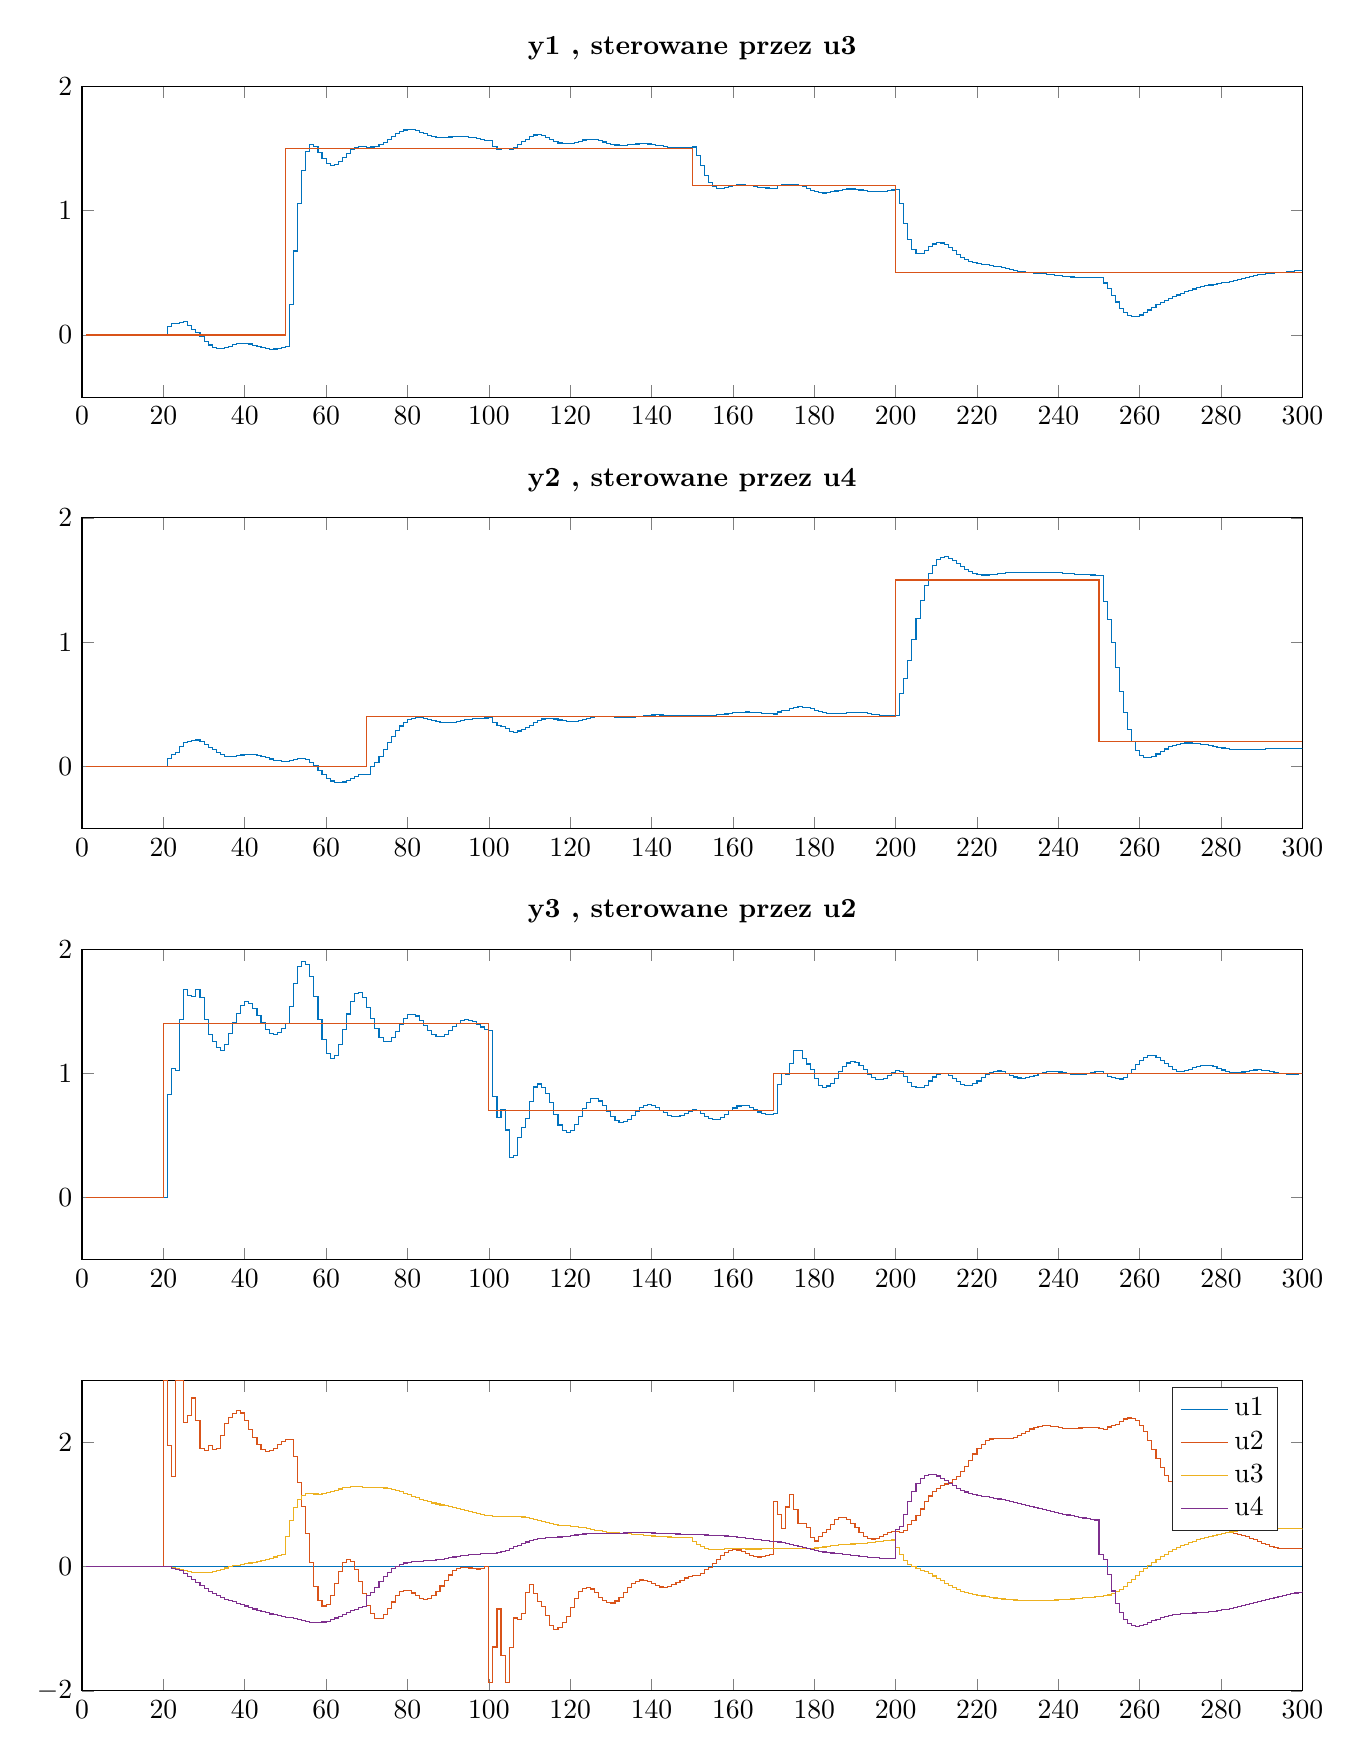
\begin{tikzpicture}

\begin{axis}[%
width=6.102in,
height=1.553in,
at={(1.024in,7.552in)},
scale only axis,
xmin=0,
xmax=300,
ymin=-0.5,
ymax=2,
axis background/.style={fill=white},
title style={font=\bfseries},
title={y1 , sterowane przez u3}
]
\addplot[const plot, color=mycolor1, forget plot] table[row sep=crcr] {%
1	0\\
2	0\\
3	0\\
4	0\\
5	0\\
6	0\\
7	0\\
8	0\\
9	0\\
10	0\\
11	0\\
12	0\\
13	0\\
14	0\\
15	0\\
16	0\\
17	0\\
18	0\\
19	0\\
20	0\\
21	0.0663597650785785\\
22	0.0948148843087075\\
23	0.089218951417981\\
24	0.103819627570907\\
25	0.105263340654856\\
26	0.0770887924563987\\
27	0.0444794289710173\\
28	0.0182654020500992\\
29	-0.0136213173212693\\
30	-0.0511469709731481\\
31	-0.0807884566101225\\
32	-0.0981278717589569\\
33	-0.107791059071515\\
34	-0.11043034602781\\
35	-0.104186925896686\\
36	-0.0922060070675766\\
37	-0.0802705782471116\\
38	-0.0713294110572463\\
39	-0.0663202625612846\\
40	-0.066552966371894\\
41	-0.0724976637659185\\
42	-0.0824048575501205\\
43	-0.093571427579295\\
44	-0.1037834827921\\
45	-0.111256106967091\\
46	-0.114539898907142\\
47	-0.113132176580923\\
48	-0.107730385014261\\
49	-0.0997485652921816\\
50	-0.0908312714024284\\
51	0.247645035418085\\
52	0.67548612528444\\
53	1.05570606519687\\
54	1.32553566580239\\
55	1.47699929321086\\
56	1.53026431593774\\
57	1.51670793016797\\
58	1.4702931401956\\
59	1.41963001254666\\
60	1.38260853896729\\
61	1.36687885084737\\
62	1.37290753360315\\
63	1.39607177812431\\
64	1.42858308571416\\
65	1.46220805581163\\
66	1.49047048679693\\
67	1.50943521194962\\
68	1.51779009600017\\
69	1.51674482914686\\
70	1.50944513564728\\
71	1.51328671947939\\
72	1.51946500451918\\
73	1.53167777172329\\
74	1.55072317236026\\
75	1.57418496511981\\
76	1.59871191403788\\
77	1.62111553727587\\
78	1.63884139276386\\
79	1.6501062904759\\
80	1.65412675845604\\
81	1.65132395447184\\
82	1.64314636012092\\
83	1.6316346483459\\
84	1.61902650814705\\
85	1.60741141833894\\
86	1.59837533031227\\
87	1.59274739698347\\
88	1.59055628137561\\
89	1.59115221747659\\
90	1.59341695127192\\
91	1.59603565382792\\
92	1.59779268831295\\
93	1.59781399163978\\
94	1.59570154193553\\
95	1.5915551908008\\
96	1.58589573330473\\
97	1.57950848157423\\
98	1.57324506398584\\
99	1.5678337468926\\
100	1.56373847094554\\
101	1.51889431273706\\
102	1.49624129120953\\
103	1.50198749915628\\
104	1.499518910839\\
105	1.49235757258592\\
106	1.50496143321856\\
107	1.53243385976334\\
108	1.55664534020539\\
109	1.57631527404413\\
110	1.59584137284055\\
111	1.60945022211578\\
112	1.61076740045269\\
113	1.60246255764002\\
114	1.58966988731152\\
115	1.57415813820241\\
116	1.55788182279522\\
117	1.54502539792793\\
118	1.53850852568422\\
119	1.53820796772538\\
120	1.54286822619476\\
121	1.55112764594715\\
122	1.56079035434422\\
123	1.56906565843633\\
124	1.57387032503117\\
125	1.57432892465506\\
126	1.57043051676332\\
127	1.56290705380263\\
128	1.55326551337784\\
129	1.54340113792994\\
130	1.53500659134652\\
131	1.52924956221302\\
132	1.52667440149469\\
133	1.52713333070325\\
134	1.52982861411077\\
135	1.53355821618879\\
136	1.53704109567711\\
137	1.53918234606464\\
138	1.53926628487026\\
139	1.53707968705321\\
140	1.53291975235574\\
141	1.52747678067054\\
142	1.52164609272835\\
143	1.51632579394615\\
144	1.51223230291884\\
145	1.50976530325796\\
146	1.50895333226797\\
147	1.50948614611286\\
148	1.51081374755769\\
149	1.5122837594289\\
150	1.51328776842713\\
151	1.44732892070499\\
152	1.36197222806224\\
153	1.28452812112307\\
154	1.22783687423923\\
155	1.1940446121745\\
156	1.17978929448763\\
157	1.17944195786565\\
158	1.18669869868248\\
159	1.19607592453561\\
160	1.20395724504882\\
161	1.20853444669849\\
162	1.20927683487537\\
163	1.20661700373924\\
164	1.20167403029781\\
165	1.19579641039176\\
166	1.19016958643392\\
167	1.18566267218745\\
168	1.18277585024014\\
169	1.18159546318691\\
170	1.18183286502464\\
171	1.2010493050278\\
172	1.21158584686852\\
173	1.21003274466396\\
174	1.21142171975572\\
175	1.21380533689765\\
176	1.20655332876461\\
177	1.19189833742944\\
178	1.17796652256097\\
179	1.16579086947034\\
180	1.15398444106838\\
181	1.14542486674109\\
182	1.14307737719533\\
183	1.14583018181542\\
184	1.1513268319144\\
185	1.15851465083517\\
186	1.16619763552271\\
187	1.17224160877396\\
188	1.1751409615853\\
189	1.1748246462932\\
190	1.17185006185176\\
191	1.16694487793344\\
192	1.1612760481198\\
193	1.15629121839449\\
194	1.15310480617922\\
195	1.15223948024389\\
196	1.15374892449327\\
197	1.1572685902654\\
198	1.16202168286395\\
199	1.16701954005344\\
200	1.17135562123921\\
201	1.05707114787775\\
202	0.90056660155475\\
203	0.767623511788394\\
204	0.685903828072146\\
205	0.653508255689599\\
206	0.656925996349304\\
207	0.68035204114911\\
208	0.709104320863524\\
209	0.731928972787946\\
210	0.742763012346622\\
211	0.740359373957944\\
212	0.726441440614856\\
213	0.704278154301278\\
214	0.677876906781859\\
215	0.651088469258188\\
216	0.626796906624646\\
217	0.60667899136181\\
218	0.59134958841399\\
219	0.580521816058353\\
220	0.573211653199687\\
221	0.568091599237729\\
222	0.563854771554107\\
223	0.559444261562831\\
224	0.55417641913051\\
225	0.547804391968128\\
226	0.540490879758719\\
227	0.532683253096189\\
228	0.524951175251824\\
229	0.517838591296793\\
230	0.511743394110954\\
231	0.506838018062059\\
232	0.503051504408071\\
233	0.500112742333835\\
234	0.497632122361246\\
235	0.495197985799044\\
236	0.49246944505053\\
237	0.489246602371496\\
238	0.485502791163947\\
239	0.48137540557578\\
240	0.477122757235606\\
241	0.47305930406398\\
242	0.46948407002974\\
243	0.466618154467285\\
244	0.464564277040584\\
245	0.463294753466065\\
246	0.462667483418053\\
247	0.462464123204833\\
248	0.462440608524785\\
249	0.462378254120703\\
250	0.462124613500703\\
251	0.418100056312603\\
252	0.371366788957012\\
253	0.31947360367896\\
254	0.264958028217455\\
255	0.215686397123649\\
256	0.177995266121234\\
257	0.154703735989939\\
258	0.145540990249798\\
259	0.148578638701481\\
260	0.161036571696243\\
261	0.179546329572734\\
262	0.200828625004059\\
263	0.222453075250383\\
264	0.242973492175297\\
265	0.261686387256764\\
266	0.278486030900133\\
267	0.293726119725733\\
268	0.307923583099531\\
269	0.321480979090001\\
270	0.334591672963073\\
271	0.347248279841715\\
272	0.359267150132083\\
273	0.370360763125118\\
274	0.380264156080766\\
275	0.388843827303371\\
276	0.396145124538733\\
277	0.402393373858642\\
278	0.407961066779506\\
279	0.413296964350805\\
280	0.418831919463395\\
281	0.424893595001611\\
282	0.431650281798924\\
283	0.439088390590812\\
284	0.447025685558661\\
285	0.455158676689678\\
286	0.463131900104697\\
287	0.470610938513854\\
288	0.477344125528952\\
289	0.483202693194562\\
290	0.488192942408533\\
291	0.49243979065122\\
292	0.496148007306508\\
293	0.499551722392059\\
294	0.502863569915981\\
295	0.506233688305425\\
296	0.509726149703224\\
297	0.513316059725275\\
298	0.516905710765042\\
299	0.520354370605727\\
300	0.523514135692064\\
};
\addplot[const plot, color=mycolor2, forget plot] table[row sep=crcr] {%
1	0\\
2	0\\
3	0\\
4	0\\
5	0\\
6	0\\
7	0\\
8	0\\
9	0\\
10	0\\
11	0\\
12	0\\
13	0\\
14	0\\
15	0\\
16	0\\
17	0\\
18	0\\
19	0\\
20	0\\
21	0\\
22	0\\
23	0\\
24	0\\
25	0\\
26	0\\
27	0\\
28	0\\
29	0\\
30	0\\
31	0\\
32	0\\
33	0\\
34	0\\
35	0\\
36	0\\
37	0\\
38	0\\
39	0\\
40	0\\
41	0\\
42	0\\
43	0\\
44	0\\
45	0\\
46	0\\
47	0\\
48	0\\
49	0\\
50	1.5\\
51	1.5\\
52	1.5\\
53	1.5\\
54	1.5\\
55	1.5\\
56	1.5\\
57	1.5\\
58	1.5\\
59	1.5\\
60	1.5\\
61	1.5\\
62	1.5\\
63	1.5\\
64	1.5\\
65	1.5\\
66	1.5\\
67	1.5\\
68	1.5\\
69	1.5\\
70	1.5\\
71	1.5\\
72	1.5\\
73	1.5\\
74	1.5\\
75	1.5\\
76	1.5\\
77	1.5\\
78	1.5\\
79	1.5\\
80	1.5\\
81	1.5\\
82	1.5\\
83	1.5\\
84	1.5\\
85	1.5\\
86	1.5\\
87	1.5\\
88	1.5\\
89	1.5\\
90	1.5\\
91	1.5\\
92	1.5\\
93	1.5\\
94	1.5\\
95	1.5\\
96	1.5\\
97	1.5\\
98	1.5\\
99	1.5\\
100	1.5\\
101	1.5\\
102	1.5\\
103	1.5\\
104	1.5\\
105	1.5\\
106	1.5\\
107	1.5\\
108	1.5\\
109	1.5\\
110	1.5\\
111	1.5\\
112	1.5\\
113	1.5\\
114	1.5\\
115	1.5\\
116	1.5\\
117	1.5\\
118	1.5\\
119	1.5\\
120	1.5\\
121	1.5\\
122	1.5\\
123	1.5\\
124	1.5\\
125	1.5\\
126	1.5\\
127	1.5\\
128	1.5\\
129	1.5\\
130	1.5\\
131	1.5\\
132	1.5\\
133	1.5\\
134	1.5\\
135	1.5\\
136	1.5\\
137	1.5\\
138	1.5\\
139	1.5\\
140	1.5\\
141	1.5\\
142	1.5\\
143	1.5\\
144	1.5\\
145	1.5\\
146	1.5\\
147	1.5\\
148	1.5\\
149	1.5\\
150	1.2\\
151	1.2\\
152	1.2\\
153	1.2\\
154	1.2\\
155	1.2\\
156	1.2\\
157	1.2\\
158	1.2\\
159	1.2\\
160	1.2\\
161	1.2\\
162	1.2\\
163	1.2\\
164	1.2\\
165	1.2\\
166	1.2\\
167	1.2\\
168	1.2\\
169	1.2\\
170	1.2\\
171	1.2\\
172	1.2\\
173	1.2\\
174	1.2\\
175	1.2\\
176	1.2\\
177	1.2\\
178	1.2\\
179	1.2\\
180	1.2\\
181	1.2\\
182	1.2\\
183	1.2\\
184	1.2\\
185	1.2\\
186	1.2\\
187	1.2\\
188	1.2\\
189	1.2\\
190	1.2\\
191	1.2\\
192	1.2\\
193	1.2\\
194	1.2\\
195	1.2\\
196	1.2\\
197	1.2\\
198	1.2\\
199	1.2\\
200	0.5\\
201	0.5\\
202	0.5\\
203	0.5\\
204	0.5\\
205	0.5\\
206	0.5\\
207	0.5\\
208	0.5\\
209	0.5\\
210	0.5\\
211	0.5\\
212	0.5\\
213	0.5\\
214	0.5\\
215	0.5\\
216	0.5\\
217	0.5\\
218	0.5\\
219	0.5\\
220	0.5\\
221	0.5\\
222	0.5\\
223	0.5\\
224	0.5\\
225	0.5\\
226	0.5\\
227	0.5\\
228	0.5\\
229	0.5\\
230	0.5\\
231	0.5\\
232	0.5\\
233	0.5\\
234	0.5\\
235	0.5\\
236	0.5\\
237	0.5\\
238	0.5\\
239	0.5\\
240	0.5\\
241	0.5\\
242	0.5\\
243	0.5\\
244	0.5\\
245	0.5\\
246	0.5\\
247	0.5\\
248	0.5\\
249	0.5\\
250	0.5\\
251	0.5\\
252	0.5\\
253	0.5\\
254	0.5\\
255	0.5\\
256	0.5\\
257	0.5\\
258	0.5\\
259	0.5\\
260	0.5\\
261	0.5\\
262	0.5\\
263	0.5\\
264	0.5\\
265	0.5\\
266	0.5\\
267	0.5\\
268	0.5\\
269	0.5\\
270	0.5\\
271	0.5\\
272	0.5\\
273	0.5\\
274	0.5\\
275	0.5\\
276	0.5\\
277	0.5\\
278	0.5\\
279	0.5\\
280	0.5\\
281	0.5\\
282	0.5\\
283	0.5\\
284	0.5\\
285	0.5\\
286	0.5\\
287	0.5\\
288	0.5\\
289	0.5\\
290	0.5\\
291	0.5\\
292	0.5\\
293	0.5\\
294	0.5\\
295	0.5\\
296	0.5\\
297	0.5\\
298	0.5\\
299	0.5\\
300	0.5\\
};
\end{axis}

\begin{axis}[%
width=6.102in,
height=1.553in,
at={(1.024in,5.395in)},
scale only axis,
xmin=0,
xmax=300,
ymin=-0.5,
ymax=2,
axis background/.style={fill=white},
title style={font=\bfseries},
title={y2 , sterowane przez u4}
]
\addplot[const plot, color=mycolor1, forget plot] table[row sep=crcr] {%
1	0\\
2	0\\
3	0\\
4	0\\
5	0\\
6	0\\
7	0\\
8	0\\
9	0\\
10	0\\
11	0\\
12	0\\
13	0\\
14	0\\
15	0\\
16	0\\
17	0\\
18	0\\
19	0\\
20	0\\
21	0.0612158143362928\\
22	0.0985078430383128\\
23	0.114085610426131\\
24	0.156752978298174\\
25	0.193106686302819\\
26	0.203444213828835\\
27	0.207617645154057\\
28	0.211836581440369\\
29	0.202670057896908\\
30	0.179478067270503\\
31	0.154495769762085\\
32	0.132366607360176\\
33	0.110952299916149\\
34	0.0927324892872449\\
35	0.082439015746444\\
36	0.0797828671113494\\
37	0.0814563955142404\\
38	0.0857214589040287\\
39	0.0914071281713924\\
40	0.0959803333354381\\
41	0.0971033681136073\\
42	0.0942805828045651\\
43	0.0880912505100276\\
44	0.0792693962105173\\
45	0.0689893190766994\\
46	0.0589378287911803\\
47	0.0505852082032534\\
48	0.0446972013695936\\
49	0.0414568344307307\\
50	0.0405879612936637\\
51	0.0465562927922251\\
52	0.0572909393405645\\
53	0.0642598632574575\\
54	0.06271276839559\\
55	0.0525088816781333\\
56	0.0331386192625341\\
57	0.00454099701937555\\
58	-0.0298392756057023\\
59	-0.0645126942105634\\
60	-0.0949280680524921\\
61	-0.117802416907222\\
62	-0.130664604093302\\
63	-0.132707703168537\\
64	-0.125433602317846\\
65	-0.111890811375451\\
66	-0.0956230143978562\\
67	-0.0801531227880822\\
68	-0.0684945418302017\\
69	-0.0624792137363066\\
70	-0.0624290074463734\\
71	-0.00381571987336616\\
72	0.0341701164343098\\
73	0.080175431123899\\
74	0.134577303986069\\
75	0.189304864802683\\
76	0.2405175830751\\
77	0.286151842160077\\
78	0.324592807756461\\
79	0.354679836749445\\
80	0.375835237223816\\
81	0.388228540596793\\
82	0.392752898634623\\
83	0.390853603197619\\
84	0.384386814324844\\
85	0.375452306213075\\
86	0.366115846944884\\
87	0.358120708701492\\
88	0.352701465381012\\
89	0.350494413127013\\
90	0.351522018342512\\
91	0.355274128375738\\
92	0.360883356298275\\
93	0.367339300360369\\
94	0.373689109102581\\
95	0.379199524641627\\
96	0.383459880395232\\
97	0.386406974576019\\
98	0.388274208997345\\
99	0.389488961361697\\
100	0.390546627976987\\
101	0.352964260345975\\
102	0.328255059070342\\
103	0.322981397274355\\
104	0.305334645617871\\
105	0.281335760626078\\
106	0.27531511977936\\
107	0.284643445616035\\
108	0.295672997793311\\
109	0.309720831113889\\
110	0.331328027600265\\
111	0.354250533220717\\
112	0.370945914456975\\
113	0.381343148969601\\
114	0.3870784642609\\
115	0.387078744956509\\
116	0.381472800821834\\
117	0.373537113375038\\
118	0.366440199877764\\
119	0.361535168657645\\
120	0.359756322654787\\
121	0.362001191151597\\
122	0.368002431001561\\
123	0.376272313060526\\
124	0.385145701850116\\
125	0.393240476975755\\
126	0.399343741447864\\
127	0.402628888861827\\
128	0.403023844601089\\
129	0.401143621086957\\
130	0.39795069079182\\
131	0.39453461427463\\
132	0.391954466480443\\
133	0.390999756079583\\
134	0.391999016781025\\
135	0.3948101306355\\
136	0.398924589472849\\
137	0.403597154099537\\
138	0.408008090819439\\
139	0.411451503626957\\
140	0.413482420706719\\
141	0.413979184399988\\
142	0.413133142486069\\
143	0.411383415777391\\
144	0.409304576272876\\
145	0.40747102158301\\
146	0.406335886547032\\
147	0.406150434533929\\
148	0.40693233192869\\
149	0.408483915874938\\
150	0.410454657472248\\
151	0.411383911569178\\
152	0.41108273610577\\
153	0.410767581136647\\
154	0.411109349234952\\
155	0.41209612458881\\
156	0.414013441229726\\
157	0.417228576248746\\
158	0.42148941263563\\
159	0.4261135590819\\
160	0.430500609717071\\
161	0.434146493198138\\
162	0.436535551449229\\
163	0.437331084174032\\
164	0.436556487177441\\
165	0.434511867204103\\
166	0.431631725694201\\
167	0.428435469757722\\
168	0.425460261045186\\
169	0.423129277908522\\
170	0.421662281829148\\
171	0.437755888779953\\
172	0.449299247455602\\
173	0.453226706768106\\
174	0.462767916266364\\
175	0.474898540486286\\
176	0.478806672240494\\
177	0.475364643933552\\
178	0.470337959406712\\
179	0.463255029972093\\
180	0.452403872643024\\
181	0.440772306001194\\
182	0.431910329536334\\
183	0.426106747959011\\
184	0.422811893392684\\
185	0.422509073407875\\
186	0.425046684135978\\
187	0.428837255137748\\
188	0.432300050963755\\
189	0.434643669329784\\
190	0.435311367066424\\
191	0.433845422213619\\
192	0.430378274153145\\
193	0.425644147257615\\
194	0.420504684178975\\
195	0.415716107260219\\
196	0.411942478899722\\
197	0.409634706701807\\
198	0.408857472930346\\
199	0.409317502459848\\
200	0.410521793077092\\
201	0.584201207435534\\
202	0.707294920432433\\
203	0.855169277976701\\
204	1.0241777128896\\
205	1.18726515747465\\
206	1.33200879987545\\
207	1.4535929945052\\
208	1.54925142637187\\
209	1.61805629910238\\
210	1.66149346162254\\
211	1.6829148250694\\
212	1.68640628516165\\
213	1.67629929747112\\
214	1.657127864954\\
215	1.63327039944467\\
216	1.60844352395047\\
217	1.58551470147439\\
218	1.56651198824923\\
219	1.5525733224913\\
220	1.54393969841404\\
221	1.54013158168181\\
222	1.54020518906174\\
223	1.54296960256401\\
224	1.54718608374936\\
225	1.55176722727789\\
226	1.55591611268855\\
227	1.55917003699591\\
228	1.56137796791282\\
229	1.56263976234429\\
230	1.56321193243913\\
231	1.56339739178289\\
232	1.5634521068013\\
233	1.56352760421918\\
234	1.56364962221419\\
235	1.56373003245784\\
236	1.56360751715731\\
237	1.56310390768404\\
238	1.56207872110625\\
239	1.56046917428531\\
240	1.55830913950148\\
241	1.55572444126614\\
242	1.55290666294778\\
243	1.55007317059644\\
244	1.54742377228626\\
245	1.54510360649504\\
246	1.54317949806931\\
247	1.54163391324204\\
248	1.54037660564565\\
249	1.53927002713275\\
250	1.53816199104827\\
251	1.33039606035631\\
252	1.17936754029042\\
253	0.999583821221328\\
254	0.797336474457079\\
255	0.60458061947095\\
256	0.436674263282473\\
257	0.300127604300298\\
258	0.197294810792607\\
259	0.127188007694998\\
260	0.0862456370224834\\
261	0.0690482268170427\\
262	0.0693669528098735\\
263	0.0812498720578617\\
264	0.0995428181941474\\
265	0.120049751936233\\
266	0.139705571364647\\
267	0.156634102031015\\
268	0.169937872270096\\
269	0.179396586821207\\
270	0.18524239327678\\
271	0.187970214722086\\
272	0.188147084988279\\
273	0.186288004877757\\
274	0.18282779228874\\
275	0.178136314244293\\
276	0.172539462069785\\
277	0.166349709682578\\
278	0.159897972885074\\
279	0.153541422746588\\
280	0.147641939120125\\
281	0.142530514218481\\
282	0.138468904350952\\
283	0.135613773930749\\
284	0.133993022087399\\
285	0.133504259902504\\
286	0.133936358590537\\
287	0.135007837681844\\
288	0.136414691161039\\
289	0.137879464062608\\
290	0.139192006492233\\
291	0.140234098373182\\
292	0.140984820990993\\
293	0.141507803956453\\
294	0.14192438208226\\
295	0.142379058229615\\
296	0.143004959953399\\
297	0.143896238657693\\
298	0.145092041010886\\
299	0.146573876362374\\
300	0.148275423261956\\
};
\addplot[const plot, color=mycolor2, forget plot] table[row sep=crcr] {%
1	0\\
2	0\\
3	0\\
4	0\\
5	0\\
6	0\\
7	0\\
8	0\\
9	0\\
10	0\\
11	0\\
12	0\\
13	0\\
14	0\\
15	0\\
16	0\\
17	0\\
18	0\\
19	0\\
20	0\\
21	0\\
22	0\\
23	0\\
24	0\\
25	0\\
26	0\\
27	0\\
28	0\\
29	0\\
30	0\\
31	0\\
32	0\\
33	0\\
34	0\\
35	0\\
36	0\\
37	0\\
38	0\\
39	0\\
40	0\\
41	0\\
42	0\\
43	0\\
44	0\\
45	0\\
46	0\\
47	0\\
48	0\\
49	0\\
50	0\\
51	0\\
52	0\\
53	0\\
54	0\\
55	0\\
56	0\\
57	0\\
58	0\\
59	0\\
60	0\\
61	0\\
62	0\\
63	0\\
64	0\\
65	0\\
66	0\\
67	0\\
68	0\\
69	0\\
70	0.4\\
71	0.4\\
72	0.4\\
73	0.4\\
74	0.4\\
75	0.4\\
76	0.4\\
77	0.4\\
78	0.4\\
79	0.4\\
80	0.4\\
81	0.4\\
82	0.4\\
83	0.4\\
84	0.4\\
85	0.4\\
86	0.4\\
87	0.4\\
88	0.4\\
89	0.4\\
90	0.4\\
91	0.4\\
92	0.4\\
93	0.4\\
94	0.4\\
95	0.4\\
96	0.4\\
97	0.4\\
98	0.4\\
99	0.4\\
100	0.4\\
101	0.4\\
102	0.4\\
103	0.4\\
104	0.4\\
105	0.4\\
106	0.4\\
107	0.4\\
108	0.4\\
109	0.4\\
110	0.4\\
111	0.4\\
112	0.4\\
113	0.4\\
114	0.4\\
115	0.4\\
116	0.4\\
117	0.4\\
118	0.4\\
119	0.4\\
120	0.4\\
121	0.4\\
122	0.4\\
123	0.4\\
124	0.4\\
125	0.4\\
126	0.4\\
127	0.4\\
128	0.4\\
129	0.4\\
130	0.4\\
131	0.4\\
132	0.4\\
133	0.4\\
134	0.4\\
135	0.4\\
136	0.4\\
137	0.4\\
138	0.4\\
139	0.4\\
140	0.4\\
141	0.4\\
142	0.4\\
143	0.4\\
144	0.4\\
145	0.4\\
146	0.4\\
147	0.4\\
148	0.4\\
149	0.4\\
150	0.4\\
151	0.4\\
152	0.4\\
153	0.4\\
154	0.4\\
155	0.4\\
156	0.4\\
157	0.4\\
158	0.4\\
159	0.4\\
160	0.4\\
161	0.4\\
162	0.4\\
163	0.4\\
164	0.4\\
165	0.4\\
166	0.4\\
167	0.4\\
168	0.4\\
169	0.4\\
170	0.4\\
171	0.4\\
172	0.4\\
173	0.4\\
174	0.4\\
175	0.4\\
176	0.4\\
177	0.4\\
178	0.4\\
179	0.4\\
180	0.4\\
181	0.4\\
182	0.4\\
183	0.4\\
184	0.4\\
185	0.4\\
186	0.4\\
187	0.4\\
188	0.4\\
189	0.4\\
190	0.4\\
191	0.4\\
192	0.4\\
193	0.4\\
194	0.4\\
195	0.4\\
196	0.4\\
197	0.4\\
198	0.4\\
199	0.4\\
200	1.5\\
201	1.5\\
202	1.5\\
203	1.5\\
204	1.5\\
205	1.5\\
206	1.5\\
207	1.5\\
208	1.5\\
209	1.5\\
210	1.5\\
211	1.5\\
212	1.5\\
213	1.5\\
214	1.5\\
215	1.5\\
216	1.5\\
217	1.5\\
218	1.5\\
219	1.5\\
220	1.5\\
221	1.5\\
222	1.5\\
223	1.5\\
224	1.5\\
225	1.5\\
226	1.5\\
227	1.5\\
228	1.5\\
229	1.5\\
230	1.5\\
231	1.5\\
232	1.5\\
233	1.5\\
234	1.5\\
235	1.5\\
236	1.5\\
237	1.5\\
238	1.5\\
239	1.5\\
240	1.5\\
241	1.5\\
242	1.5\\
243	1.5\\
244	1.5\\
245	1.5\\
246	1.5\\
247	1.5\\
248	1.5\\
249	1.5\\
250	0.2\\
251	0.2\\
252	0.2\\
253	0.2\\
254	0.2\\
255	0.2\\
256	0.2\\
257	0.2\\
258	0.2\\
259	0.2\\
260	0.2\\
261	0.2\\
262	0.2\\
263	0.2\\
264	0.2\\
265	0.2\\
266	0.2\\
267	0.2\\
268	0.2\\
269	0.2\\
270	0.2\\
271	0.2\\
272	0.2\\
273	0.2\\
274	0.2\\
275	0.2\\
276	0.2\\
277	0.2\\
278	0.2\\
279	0.2\\
280	0.2\\
281	0.2\\
282	0.2\\
283	0.2\\
284	0.2\\
285	0.2\\
286	0.2\\
287	0.2\\
288	0.2\\
289	0.2\\
290	0.2\\
291	0.2\\
292	0.2\\
293	0.2\\
294	0.2\\
295	0.2\\
296	0.2\\
297	0.2\\
298	0.2\\
299	0.2\\
300	0.2\\
};
\end{axis}

\begin{axis}[%
width=6.102in,
height=1.553in,
at={(1.024in,3.239in)},
scale only axis,
xmin=0,
xmax=300,
ymin=-0.5,
ymax=2,
axis background/.style={fill=white},
title style={font=\bfseries},
title={y3 , sterowane przez u2}
]
\addplot[const plot, color=mycolor1, forget plot] table[row sep=crcr] {%
1	0\\
2	0\\
3	0\\
4	0\\
5	0\\
6	0\\
7	0\\
8	0\\
9	0\\
10	0\\
11	0\\
12	0\\
13	0\\
14	0\\
15	0\\
16	0\\
17	0\\
18	0\\
19	0\\
20	0\\
21	0.82628561460347\\
22	1.03825320842876\\
23	1.02362014286053\\
24	1.43504611178129\\
25	1.67692382252678\\
26	1.62633665181787\\
27	1.61767690822868\\
28	1.67829943357419\\
29	1.60712787734862\\
30	1.43145078353962\\
31	1.31079773769169\\
32	1.25669092318886\\
33	1.20710655292484\\
34	1.18416842779207\\
35	1.2309158987726\\
36	1.32061309204105\\
37	1.40703595225894\\
38	1.48139105307679\\
39	1.54331649901828\\
40	1.57482950220253\\
41	1.56469718997088\\
42	1.52394466605226\\
43	1.46861408947028\\
44	1.40861390895872\\
45	1.35470442842243\\
46	1.31988150814158\\
47	1.31093337574858\\
48	1.32583669875088\\
49	1.35856123016574\\
50	1.4015010474881\\
51	1.53624101935613\\
52	1.72453423480645\\
53	1.85740331837239\\
54	1.90124317770571\\
55	1.87617734677734\\
56	1.78169756664667\\
57	1.6195766868578\\
58	1.43139606780827\\
59	1.2691373010035\\
60	1.16035055080118\\
61	1.11598592482405\\
62	1.14186832244486\\
63	1.22945334125636\\
64	1.35203248301553\\
65	1.47782578975722\\
66	1.58092157969881\\
67	1.64238259877515\\
68	1.65165521826445\\
69	1.6105171173053\\
70	1.53249398101464\\
71	1.44379741918938\\
72	1.35834706940403\\
73	1.29076488793583\\
74	1.25620450123803\\
75	1.25820304402045\\
76	1.28891867440387\\
77	1.33748269382078\\
78	1.39226820890696\\
79	1.44014500082727\\
80	1.46994872449459\\
81	1.47661322233372\\
82	1.4611190246485\\
83	1.4285098071654\\
84	1.38682201082064\\
85	1.3457516507824\\
86	1.31411621086063\\
87	1.29767871815943\\
88	1.29843930977788\\
89	1.31477969971834\\
90	1.34198442707061\\
91	1.37340441607181\\
92	1.40214119561209\\
93	1.4225790602663\\
94	1.43136846970578\\
95	1.42787911218146\\
96	1.41411789973025\\
97	1.39407168279182\\
98	1.37265332909672\\
99	1.35457801359375\\
100	1.34341467977376\\
101	0.815572802083233\\
102	0.647549197275044\\
103	0.711069298852707\\
104	0.543784589892488\\
105	0.319054379865405\\
106	0.339465933511164\\
107	0.483247646736859\\
108	0.563203534554637\\
109	0.638462691667516\\
110	0.775831793804524\\
111	0.890220306272589\\
112	0.913807178472119\\
113	0.88501732060605\\
114	0.83983664277336\\
115	0.765779740877514\\
116	0.667887822232023\\
117	0.584448976979396\\
118	0.538223278485781\\
119	0.525208604830949\\
120	0.541727912817197\\
121	0.587937524644069\\
122	0.652705454753299\\
123	0.716645912408085\\
124	0.766012359907312\\
125	0.794466172051421\\
126	0.798211650430108\\
127	0.777375072631749\\
128	0.73887196835569\\
129	0.6935013200418\\
130	0.651374922996283\\
131	0.620524891622525\\
132	0.606544508191119\\
133	0.611149037721525\\
134	0.631549883412289\\
135	0.661839658174905\\
136	0.69489199358243\\
137	0.723717541116411\\
138	0.742717305157497\\
139	0.748894357059926\\
140	0.742334894222407\\
141	0.725775753318661\\
142	0.70371964491312\\
143	0.681395758494634\\
144	0.663619886051654\\
145	0.653776646711128\\
146	0.65323679772409\\
147	0.661295583287263\\
148	0.675525819804483\\
149	0.692433993490545\\
150	0.708294369269864\\
151	0.701714951543587\\
152	0.676432670790604\\
153	0.65247026285929\\
154	0.637090296965798\\
155	0.628620313465653\\
156	0.630665102546657\\
157	0.646779459760368\\
158	0.672090218586061\\
159	0.69844135744769\\
160	0.721021524509259\\
161	0.736836523588503\\
162	0.742716869468256\\
163	0.7376822800856\\
164	0.724339614717172\\
165	0.706853907513178\\
166	0.689160433867806\\
167	0.674906827904428\\
168	0.667098065940567\\
169	0.66702323852188\\
170	0.673951925830519\\
171	0.910966773185114\\
172	0.999567431420443\\
173	0.990869291041878\\
174	1.07903452236241\\
175	1.18662917340965\\
176	1.18227161335713\\
177	1.11802251968387\\
178	1.07543138909632\\
179	1.03156064512904\\
180	0.960649779813996\\
181	0.901828400165072\\
182	0.886084199018604\\
183	0.897816656135728\\
184	0.921331717750524\\
185	0.960727020689919\\
186	1.0119688250721\\
187	1.05661331029581\\
188	1.08314925479821\\
189	1.0921507213125\\
190	1.08484992210149\\
191	1.06163041902789\\
192	1.0283351889506\\
193	0.994680395089692\\
194	0.967974774341122\\
195	0.952064400974032\\
196	0.949208377733229\\
197	0.959403334622247\\
198	0.979200854979451\\
199	1.00310648580863\\
200	1.025756956657\\
201	1.01811021901995\\
202	0.971775061657808\\
203	0.92354187200487\\
204	0.896937183617456\\
205	0.885270721153098\\
206	0.885898345013968\\
207	0.905356042365478\\
208	0.938548745807636\\
209	0.970311411770451\\
210	0.991765861221054\\
211	1.00151464209433\\
212	0.99817021787309\\
213	0.981503126837922\\
214	0.956623968794546\\
215	0.931389761301021\\
216	0.911817805996163\\
217	0.901672978747559\\
218	0.903305708703658\\
219	0.916627059464193\\
220	0.938464939199118\\
221	0.963956110999166\\
222	0.988210297720478\\
223	1.00702497457775\\
224	1.01744044012848\\
225	1.01847043807232\\
226	1.0112764417697\\
227	0.998582702037545\\
228	0.983889059316078\\
229	0.970767435669767\\
230	0.962151004983995\\
231	0.959724011449649\\
232	0.963675073929336\\
233	0.972843483193903\\
234	0.985100589378143\\
235	0.997864074896944\\
236	1.00867950566356\\
237	1.01573609848662\\
238	1.01818219929751\\
239	1.01619990059844\\
240	1.01086628081048\\
241	1.0038456897322\\
242	0.99698240492228\\
243	0.991892983821322\\
244	0.989650411686924\\
245	0.990614058090123\\
246	0.994423101362429\\
247	1.00014122921842\\
248	1.00650970997977\\
249	1.01224366195444\\
250	1.01630407004847\\
251	0.996887246510258\\
252	0.975883377525619\\
253	0.965542231939337\\
254	0.957775707089035\\
255	0.954690608118994\\
256	0.967442545638024\\
257	0.99608539360615\\
258	1.03159729415923\\
259	1.06842821840367\\
260	1.10353937451762\\
261	1.13082723979697\\
262	1.14430595118028\\
263	1.14293884057728\\
264	1.12921947770819\\
265	1.10639079556268\\
266	1.07875123945165\\
267	1.05189747793908\\
268	1.0308115090481\\
269	1.01828288171367\\
270	1.01504854764075\\
271	1.02021025427064\\
272	1.03126647674026\\
273	1.04460411438929\\
274	1.05657058515528\\
275	1.06432811062782\\
276	1.06621819411168\\
277	1.06193712449718\\
278	1.05254699796969\\
279	1.04013211324485\\
280	1.02719995170365\\
281	1.01610274106451\\
282	1.00859207182246\\
283	1.00551044234483\\
284	1.00668155267072\\
285	1.01104839810693\\
286	1.01699520048919\\
287	1.02274059758503\\
288	1.02672145479222\\
289	1.02790330338319\\
290	1.02595247955446\\
291	1.02123820810018\\
292	1.01468562426015\\
293	1.00753004218626\\
294	1.00103006125342\\
295	0.99620087823027\\
296	0.993624176904861\\
297	0.993368565767382\\
298	0.995024990864994\\
299	0.997837844234154\\
300	1.00089610788464\\
};
\addplot[const plot, color=mycolor2, forget plot] table[row sep=crcr] {%
1	0\\
2	0\\
3	0\\
4	0\\
5	0\\
6	0\\
7	0\\
8	0\\
9	0\\
10	0\\
11	0\\
12	0\\
13	0\\
14	0\\
15	0\\
16	0\\
17	0\\
18	0\\
19	0\\
20	1.4\\
21	1.4\\
22	1.4\\
23	1.4\\
24	1.4\\
25	1.4\\
26	1.4\\
27	1.4\\
28	1.4\\
29	1.4\\
30	1.4\\
31	1.4\\
32	1.4\\
33	1.4\\
34	1.4\\
35	1.4\\
36	1.4\\
37	1.4\\
38	1.4\\
39	1.4\\
40	1.4\\
41	1.4\\
42	1.4\\
43	1.4\\
44	1.4\\
45	1.4\\
46	1.4\\
47	1.4\\
48	1.4\\
49	1.4\\
50	1.4\\
51	1.4\\
52	1.4\\
53	1.4\\
54	1.4\\
55	1.4\\
56	1.4\\
57	1.4\\
58	1.4\\
59	1.4\\
60	1.4\\
61	1.4\\
62	1.4\\
63	1.4\\
64	1.4\\
65	1.4\\
66	1.4\\
67	1.4\\
68	1.4\\
69	1.4\\
70	1.4\\
71	1.4\\
72	1.4\\
73	1.4\\
74	1.4\\
75	1.4\\
76	1.4\\
77	1.4\\
78	1.4\\
79	1.4\\
80	1.4\\
81	1.4\\
82	1.4\\
83	1.4\\
84	1.4\\
85	1.4\\
86	1.4\\
87	1.4\\
88	1.4\\
89	1.4\\
90	1.4\\
91	1.4\\
92	1.4\\
93	1.4\\
94	1.4\\
95	1.4\\
96	1.4\\
97	1.4\\
98	1.4\\
99	1.4\\
100	0.7\\
101	0.7\\
102	0.7\\
103	0.7\\
104	0.7\\
105	0.7\\
106	0.7\\
107	0.7\\
108	0.7\\
109	0.7\\
110	0.7\\
111	0.7\\
112	0.7\\
113	0.7\\
114	0.7\\
115	0.7\\
116	0.7\\
117	0.7\\
118	0.7\\
119	0.7\\
120	0.7\\
121	0.7\\
122	0.7\\
123	0.7\\
124	0.7\\
125	0.7\\
126	0.7\\
127	0.7\\
128	0.7\\
129	0.7\\
130	0.7\\
131	0.7\\
132	0.7\\
133	0.7\\
134	0.7\\
135	0.7\\
136	0.7\\
137	0.7\\
138	0.7\\
139	0.7\\
140	0.7\\
141	0.7\\
142	0.7\\
143	0.7\\
144	0.7\\
145	0.7\\
146	0.7\\
147	0.7\\
148	0.7\\
149	0.7\\
150	0.7\\
151	0.7\\
152	0.7\\
153	0.7\\
154	0.7\\
155	0.7\\
156	0.7\\
157	0.7\\
158	0.7\\
159	0.7\\
160	0.7\\
161	0.7\\
162	0.7\\
163	0.7\\
164	0.7\\
165	0.7\\
166	0.7\\
167	0.7\\
168	0.7\\
169	0.7\\
170	1\\
171	1\\
172	1\\
173	1\\
174	1\\
175	1\\
176	1\\
177	1\\
178	1\\
179	1\\
180	1\\
181	1\\
182	1\\
183	1\\
184	1\\
185	1\\
186	1\\
187	1\\
188	1\\
189	1\\
190	1\\
191	1\\
192	1\\
193	1\\
194	1\\
195	1\\
196	1\\
197	1\\
198	1\\
199	1\\
200	1\\
201	1\\
202	1\\
203	1\\
204	1\\
205	1\\
206	1\\
207	1\\
208	1\\
209	1\\
210	1\\
211	1\\
212	1\\
213	1\\
214	1\\
215	1\\
216	1\\
217	1\\
218	1\\
219	1\\
220	1\\
221	1\\
222	1\\
223	1\\
224	1\\
225	1\\
226	1\\
227	1\\
228	1\\
229	1\\
230	1\\
231	1\\
232	1\\
233	1\\
234	1\\
235	1\\
236	1\\
237	1\\
238	1\\
239	1\\
240	1\\
241	1\\
242	1\\
243	1\\
244	1\\
245	1\\
246	1\\
247	1\\
248	1\\
249	1\\
250	1\\
251	1\\
252	1\\
253	1\\
254	1\\
255	1\\
256	1\\
257	1\\
258	1\\
259	1\\
260	1\\
261	1\\
262	1\\
263	1\\
264	1\\
265	1\\
266	1\\
267	1\\
268	1\\
269	1\\
270	1\\
271	1\\
272	1\\
273	1\\
274	1\\
275	1\\
276	1\\
277	1\\
278	1\\
279	1\\
280	1\\
281	1\\
282	1\\
283	1\\
284	1\\
285	1\\
286	1\\
287	1\\
288	1\\
289	1\\
290	1\\
291	1\\
292	1\\
293	1\\
294	1\\
295	1\\
296	1\\
297	1\\
298	1\\
299	1\\
300	1\\
};
\end{axis}

\begin{axis}[%
width=6.102in,
height=1.553in,
at={(1.024in,1.083in)},
scale only axis,
xmin=0,
xmax=300,
ymin=-2,
ymax=3,
axis background/.style={fill=white},
legend style={legend cell align=left, align=left, draw=white!15!black}
]
\addplot[const plot, color=mycolor1] table[row sep=crcr] {%
1	0\\
2	0\\
3	0\\
4	0\\
5	0\\
6	0\\
7	0\\
8	0\\
9	0\\
10	0\\
11	0\\
12	0\\
13	0\\
14	0\\
15	0\\
16	0\\
17	0\\
18	0\\
19	0\\
20	0\\
21	0\\
22	0\\
23	0\\
24	0\\
25	0\\
26	0\\
27	0\\
28	0\\
29	0\\
30	0\\
31	0\\
32	0\\
33	0\\
34	0\\
35	0\\
36	0\\
37	0\\
38	0\\
39	0\\
40	0\\
41	0\\
42	0\\
43	0\\
44	0\\
45	0\\
46	0\\
47	0\\
48	0\\
49	0\\
50	0\\
51	0\\
52	0\\
53	0\\
54	0\\
55	0\\
56	0\\
57	0\\
58	0\\
59	0\\
60	0\\
61	0\\
62	0\\
63	0\\
64	0\\
65	0\\
66	0\\
67	0\\
68	0\\
69	0\\
70	0\\
71	0\\
72	0\\
73	0\\
74	0\\
75	0\\
76	0\\
77	0\\
78	0\\
79	0\\
80	0\\
81	0\\
82	0\\
83	0\\
84	0\\
85	0\\
86	0\\
87	0\\
88	0\\
89	0\\
90	0\\
91	0\\
92	0\\
93	0\\
94	0\\
95	0\\
96	0\\
97	0\\
98	0\\
99	0\\
100	0\\
101	0\\
102	0\\
103	0\\
104	0\\
105	0\\
106	0\\
107	0\\
108	0\\
109	0\\
110	0\\
111	0\\
112	0\\
113	0\\
114	0\\
115	0\\
116	0\\
117	0\\
118	0\\
119	0\\
120	0\\
121	0\\
122	0\\
123	0\\
124	0\\
125	0\\
126	0\\
127	0\\
128	0\\
129	0\\
130	0\\
131	0\\
132	0\\
133	0\\
134	0\\
135	0\\
136	0\\
137	0\\
138	0\\
139	0\\
140	0\\
141	0\\
142	0\\
143	0\\
144	0\\
145	0\\
146	0\\
147	0\\
148	0\\
149	0\\
150	0\\
151	0\\
152	0\\
153	0\\
154	0\\
155	0\\
156	0\\
157	0\\
158	0\\
159	0\\
160	0\\
161	0\\
162	0\\
163	0\\
164	0\\
165	0\\
166	0\\
167	0\\
168	0\\
169	0\\
170	0\\
171	0\\
172	0\\
173	0\\
174	0\\
175	0\\
176	0\\
177	0\\
178	0\\
179	0\\
180	0\\
181	0\\
182	0\\
183	0\\
184	0\\
185	0\\
186	0\\
187	0\\
188	0\\
189	0\\
190	0\\
191	0\\
192	0\\
193	0\\
194	0\\
195	0\\
196	0\\
197	0\\
198	0\\
199	0\\
200	0\\
201	0\\
202	0\\
203	0\\
204	0\\
205	0\\
206	0\\
207	0\\
208	0\\
209	0\\
210	0\\
211	0\\
212	0\\
213	0\\
214	0\\
215	0\\
216	0\\
217	0\\
218	0\\
219	0\\
220	0\\
221	0\\
222	0\\
223	0\\
224	0\\
225	0\\
226	0\\
227	0\\
228	0\\
229	0\\
230	0\\
231	0\\
232	0\\
233	0\\
234	0\\
235	0\\
236	0\\
237	0\\
238	0\\
239	0\\
240	0\\
241	0\\
242	0\\
243	0\\
244	0\\
245	0\\
246	0\\
247	0\\
248	0\\
249	0\\
250	0\\
251	0\\
252	0\\
253	0\\
254	0\\
255	0\\
256	0\\
257	0\\
258	0\\
259	0\\
260	0\\
261	0\\
262	0\\
263	0\\
264	0\\
265	0\\
266	0\\
267	0\\
268	0\\
269	0\\
270	0\\
271	0\\
272	0\\
273	0\\
274	0\\
275	0\\
276	0\\
277	0\\
278	0\\
279	0\\
280	0\\
281	0\\
282	0\\
283	0\\
284	0\\
285	0\\
286	0\\
287	0\\
288	0\\
289	0\\
290	0\\
291	0\\
292	0\\
293	0\\
294	0\\
295	0\\
296	0\\
297	0\\
298	0\\
299	0\\
300	0\\
};
\addlegendentry{u1}

\addplot[const plot, color=mycolor2] table[row sep=crcr] {%
1	0\\
2	0\\
3	0\\
4	0\\
5	0\\
6	0\\
7	0\\
8	0\\
9	0\\
10	0\\
11	0\\
12	0\\
13	0\\
14	0\\
15	0\\
16	0\\
17	0\\
18	0\\
19	0\\
20	3\\
21	1.95\\
22	1.44837170020554\\
23	3\\
24	3\\
25	2.32007292497882\\
26	2.44000046131226\\
27	2.71545114482656\\
28	2.35495378991692\\
29	1.90034178588619\\
30	1.86765503532415\\
31	1.94512215681676\\
32	1.88323403970984\\
33	1.90087184541959\\
34	2.1069119713973\\
35	2.31136643070001\\
36	2.40789278727243\\
37	2.46831800411121\\
38	2.51144373150305\\
39	2.47287686188652\\
40	2.35110140698566\\
41	2.2099337414187\\
42	2.08203342086531\\
43	1.96694793661662\\
44	1.88128787739998\\
45	1.84835960429214\\
46	1.86449519153202\\
47	1.90818815269671\\
48	1.96307408772897\\
49	2.01589954807598\\
50	2.04923597253646\\
51	2.0494724954556\\
52	1.76630939739981\\
53	1.35238905483857\\
54	0.96123943951397\\
55	0.535759841997079\\
56	0.0651899778113698\\
57	-0.32270596666096\\
58	-0.547008087805975\\
59	-0.632928519045988\\
60	-0.606379702362378\\
61	-0.470874967924993\\
62	-0.267993051043421\\
63	-0.0722342425444429\\
64	0.0635259733797473\\
65	0.117851173138573\\
66	0.0801820920163965\\
67	-0.0464495592875948\\
68	-0.233891231010936\\
69	-0.439215329435561\\
70	-0.623137788173819\\
71	-0.755947340331716\\
72	-0.835912958207486\\
73	-0.835200652679668\\
74	-0.76987374450456\\
75	-0.674317163609238\\
76	-0.569139592634488\\
77	-0.471596404890011\\
78	-0.403650440039095\\
79	-0.377666297091084\\
80	-0.388894786035278\\
81	-0.424537600222177\\
82	-0.470526815117423\\
83	-0.510742658664064\\
84	-0.529269717203701\\
85	-0.516526166087175\\
86	-0.471512541198279\\
87	-0.399636250965943\\
88	-0.310760226774498\\
89	-0.217806222036459\\
90	-0.133861738609656\\
91	-0.068788465411612\\
92	-0.0274790145735792\\
93	-0.00970228090822104\\
94	-0.0105983975254988\\
95	-0.0218976342725175\\
96	-0.034020903272021\\
97	-0.0383492046179511\\
98	-0.028893063025941\\
99	-0.00321008657343834\\
100	-1.87010822058896\\
101	-1.29406128392761\\
102	-0.682287184578096\\
103	-1.42457261946088\\
104	-1.8681486024702\\
105	-1.29909419096416\\
106	-0.826004523926408\\
107	-0.854904402497023\\
108	-0.755218880634481\\
109	-0.414594806907609\\
110	-0.288768652597944\\
111	-0.435659506279928\\
112	-0.567419740737044\\
113	-0.640692325385369\\
114	-0.78232519139142\\
115	-0.948059210787041\\
116	-1.01141131225294\\
117	-0.974994313832562\\
118	-0.903267075600164\\
119	-0.799740958934561\\
120	-0.654506468319603\\
121	-0.507061685930477\\
122	-0.402104153207704\\
123	-0.346099444906699\\
124	-0.331683150239154\\
125	-0.359133194875081\\
126	-0.420452387853466\\
127	-0.491833907211446\\
128	-0.550327838991178\\
129	-0.583798876225323\\
130	-0.585760028566701\\
131	-0.553583543297699\\
132	-0.492988655640595\\
133	-0.417248288065686\\
134	-0.340937033137755\\
135	-0.276256575736179\\
136	-0.232431874848141\\
137	-0.214219512027045\\
138	-0.220279450220132\\
139	-0.244049638559644\\
140	-0.276279208358459\\
141	-0.307168514646272\\
142	-0.328082399136609\\
143	-0.333317477187329\\
144	-0.321246659649435\\
145	-0.29419987819758\\
146	-0.257453653445175\\
147	-0.217889852025458\\
148	-0.182475737814294\\
149	-0.15675504030645\\
150	-0.143776615322134\\
151	-0.143722283811835\\
152	-0.104440580536423\\
153	-0.0508488903665821\\
154	-0.00665672874797318\\
155	0.0467410338750541\\
156	0.117698935918715\\
157	0.184411526840625\\
158	0.231258103411947\\
159	0.261040675338897\\
160	0.274742566359769\\
161	0.267862192030637\\
162	0.243649748026261\\
163	0.213210149176795\\
164	0.185294010168717\\
165	0.164480744425373\\
166	0.155019447422933\\
167	0.159695364307114\\
168	0.176698950931817\\
169	0.200837080476047\\
170	1.04405087883854\\
171	0.841241502932772\\
172	0.616793511220633\\
173	0.960677945757157\\
174	1.16212240548385\\
175	0.915889255575913\\
176	0.700231141160239\\
177	0.694008327635774\\
178	0.63253247109396\\
179	0.472566964993659\\
180	0.412643244759004\\
181	0.47868305839664\\
182	0.546337362542374\\
183	0.59431205116231\\
184	0.673247454451956\\
185	0.760363005616226\\
186	0.798376281147811\\
187	0.786624194222755\\
188	0.752490549412378\\
189	0.698702433221001\\
190	0.623308757476602\\
191	0.546017966714553\\
192	0.488627111541234\\
193	0.455879583569787\\
194	0.445579450497932\\
195	0.457692185453856\\
196	0.487668243455633\\
197	0.523549658835101\\
198	0.553545882664386\\
199	0.570733385191232\\
200	0.571184513171825\\
201	0.553390134507581\\
202	0.587332240444028\\
203	0.675664295206836\\
204	0.749710595214548\\
205	0.821314651758287\\
206	0.928724905677015\\
207	1.04709330428606\\
208	1.13795339545747\\
209	1.20472362032376\\
210	1.26136983019986\\
211	1.30354252265954\\
212	1.33017866715475\\
213	1.35689648228627\\
214	1.39791268457326\\
215	1.45549529962372\\
216	1.52872023796364\\
217	1.61734819955605\\
218	1.71607668570358\\
219	1.81424661864155\\
220	1.90207926185172\\
221	1.97342991676488\\
222	2.0245610590807\\
223	2.05450560511626\\
224	2.06648111197221\\
225	2.06694710383885\\
226	2.06317074038271\\
227	2.06174632860467\\
228	2.06785322455741\\
229	2.08427754396217\\
230	2.11078535881034\\
231	2.14456259054923\\
232	2.18125453032879\\
233	2.21597888369089\\
234	2.24430325099265\\
235	2.26318510117735\\
236	2.27154307878442\\
237	2.27026790736182\\
238	2.26182017137274\\
239	2.24959760920092\\
240	2.23716382565577\\
241	2.22748346643178\\
242	2.22236448653107\\
243	2.22221864331629\\
244	2.22613274004371\\
245	2.23219867713138\\
246	2.23802458180521\\
247	2.24130465908192\\
248	2.24031197051592\\
249	2.2342175796302\\
250	2.22319238454722\\
251	2.20829109899727\\
252	2.24894267176637\\
253	2.27123550953527\\
254	2.28755317138159\\
255	2.33110687050192\\
256	2.37676108163339\\
257	2.39247859380521\\
258	2.38062752608259\\
259	2.34603655100402\\
260	2.27719946584503\\
261	2.16964814091881\\
262	2.03608680211346\\
263	1.89039899440644\\
264	1.74069935459087\\
265	1.59667684648153\\
266	1.46992193245465\\
267	1.36659386411282\\
268	1.28605220269796\\
269	1.22493209747688\\
270	1.17838628287114\\
271	1.13928898640888\\
272	1.09994398314567\\
273	1.05487637233743\\
274	1.00156065875775\\
275	0.939872158231849\\
276	0.871952611407074\\
277	0.80190704657386\\
278	0.734580385601499\\
279	0.674184935538413\\
280	0.623551495896524\\
281	0.583796725090544\\
282	0.554172361370238\\
283	0.532316087445901\\
284	0.514952099510268\\
285	0.498709511985929\\
286	0.480800137985626\\
287	0.459518294732737\\
288	0.434511691799587\\
289	0.406728903120405\\
290	0.378068261634119\\
291	0.350868824520352\\
292	0.327372967132724\\
293	0.309252455063045\\
294	0.297289218209124\\
295	0.291277949370514\\
296	0.290149934676147\\
297	0.292261981953745\\
298	0.295774898521481\\
299	0.299039210646304\\
300	0.300905796829323\\
};
\addlegendentry{u2}

\addplot[const plot, color=mycolor3] table[row sep=crcr] {%
1	0\\
2	0\\
3	0\\
4	0\\
5	0\\
6	0\\
7	0\\
8	0\\
9	0\\
10	0\\
11	0\\
12	0\\
13	0\\
14	0\\
15	0\\
16	0\\
17	0\\
18	0\\
19	0\\
20	0\\
21	0\\
22	-0.0121659569310727\\
23	-0.0284426896363595\\
24	-0.0432192493245108\\
25	-0.0607658651888775\\
26	-0.0783338171827527\\
27	-0.0907123734555115\\
28	-0.0975821222259247\\
29	-0.100189455452259\\
30	-0.0973877905758582\\
31	-0.0882378678528022\\
32	-0.0742791003238322\\
33	-0.0576354647781922\\
34	-0.0395092351443971\\
35	-0.0210601893571572\\
36	-0.00379975870989495\\
37	0.011368227154216\\
38	0.0245477330483935\\
39	0.0362869487714368\\
40	0.0472568400567182\\
41	0.0583528795155441\\
42	0.0705349017664309\\
43	0.0844341645878543\\
44	0.100215512018223\\
45	0.117682960070453\\
46	0.136350188301218\\
47	0.155494901318076\\
48	0.174326802042793\\
49	0.192191836352392\\
50	0.483683566905721\\
51	0.74867349057463\\
52	0.951758046224607\\
53	1.08204634051276\\
54	1.14975833064808\\
55	1.17433855967092\\
56	1.1756476170123\\
57	1.16971581397723\\
58	1.16715709871206\\
59	1.17288182184567\\
60	1.18712120521537\\
61	1.20730347328048\\
62	1.22975249294125\\
63	1.25083409262813\\
64	1.26776939219873\\
65	1.27913035611987\\
66	1.28486859731631\\
67	1.28598580900039\\
68	1.28409719492291\\
69	1.28099293085537\\
70	1.27821954711179\\
71	1.27676701939557\\
72	1.2744885397518\\
73	1.27114140091461\\
74	1.26565822617399\\
75	1.25688694077\\
76	1.24413175003737\\
77	1.22727098188242\\
78	1.20671166528247\\
79	1.18327600223037\\
80	1.15807053885585\\
81	1.13231573798017\\
82	1.10714179230127\\
83	1.08342035885363\\
84	1.0616731126589\\
85	1.04204549697104\\
86	1.02433717874468\\
87	1.00809189182642\\
88	0.992727791217984\\
89	0.977671596248848\\
90	0.962469627734399\\
91	0.94686239029249\\
92	0.930812802945236\\
93	0.91448473765166\\
94	0.898182050656249\\
95	0.882267001162065\\
96	0.867076908547511\\
97	0.852855277288323\\
98	0.839710317888126\\
99	0.827607197516959\\
100	0.816391761653079\\
101	0.805836937761273\\
102	0.803435288275237\\
103	0.804439290099109\\
104	0.804012270107283\\
105	0.804133594772738\\
106	0.805526688312636\\
107	0.804489718432332\\
108	0.798626201362695\\
109	0.788781786654429\\
110	0.775734742083094\\
111	0.759435744963062\\
112	0.740967227122511\\
113	0.722484040741447\\
114	0.705545361848322\\
115	0.690813591801877\\
116	0.678712431253294\\
117	0.669336732710877\\
118	0.662046773470677\\
119	0.655737300394036\\
120	0.649374315072454\\
121	0.64215193973217\\
122	0.633493008411772\\
123	0.623200237547784\\
124	0.611551372740193\\
125	0.599159574125084\\
126	0.586763776688842\\
127	0.575090330693151\\
128	0.564731212775391\\
129	0.55601431955283\\
130	0.548945202821972\\
131	0.543250680040609\\
132	0.538471703490665\\
133	0.534068889253521\\
134	0.529539018649504\\
135	0.524522661574251\\
136	0.518867465508153\\
137	0.512635901570495\\
138	0.506069823053264\\
139	0.49952404326146\\
140	0.493380538716209\\
141	0.487963245568544\\
142	0.483474498318207\\
143	0.479963994329186\\
144	0.477331700317863\\
145	0.475361208015179\\
146	0.473774774133201\\
147	0.472296084938372\\
148	0.470706180355481\\
149	0.468881762405118\\
150	0.411809968969114\\
151	0.359578607414621\\
152	0.319456434759159\\
153	0.293883674959498\\
154	0.281086389887971\\
155	0.27739176496283\\
156	0.278947533968159\\
157	0.282553573515001\\
158	0.285985702814427\\
159	0.288081640687067\\
160	0.288579366166914\\
161	0.287788469983556\\
162	0.286289775506313\\
163	0.284731263224136\\
164	0.283672759786531\\
165	0.283476137627586\\
166	0.284274696227394\\
167	0.286006878887705\\
168	0.288471548760572\\
169	0.291390354086337\\
170	0.294477450006073\\
171	0.297501349138003\\
172	0.297006190966651\\
173	0.294899607457885\\
174	0.293253368383967\\
175	0.291326598839818\\
176	0.288985982404511\\
177	0.28801462774596\\
178	0.289609154696639\\
179	0.293513597850952\\
180	0.299418047157405\\
181	0.307284080786042\\
182	0.316522595901316\\
183	0.326048824527858\\
184	0.335031247481619\\
185	0.34305183132757\\
186	0.349846259206362\\
187	0.355351936874451\\
188	0.359877602524603\\
189	0.363972453046864\\
190	0.368173617252867\\
191	0.372914850018265\\
192	0.378505790094663\\
193	0.38505426257159\\
194	0.392422140001264\\
195	0.400291112508316\\
196	0.408265621233256\\
197	0.415948976413555\\
198	0.423012216939787\\
199	0.429262718252486\\
200	0.306342830623755\\
201	0.194377959064123\\
202	0.103437508973856\\
203	0.0392848178201145\\
204	-0.00310338264851202\\
205	-0.0327253592652656\\
206	-0.0577701423404897\\
207	-0.0839814374097022\\
208	-0.114430545014551\\
209	-0.149760469820378\\
210	-0.188795709483776\\
211	-0.229436778867525\\
212	-0.269456613887371\\
213	-0.306964888434128\\
214	-0.340641859379115\\
215	-0.369847989717435\\
216	-0.394582927301738\\
217	-0.415310885695287\\
218	-0.432755419001208\\
219	-0.447724860354409\\
220	-0.460964700158207\\
221	-0.473044806310511\\
222	-0.484308071950766\\
223	-0.494879920081724\\
224	-0.504713788509008\\
225	-0.513655394323554\\
226	-0.521516592532202\\
227	-0.528143180621832\\
228	-0.533460262360154\\
229	-0.537489923604719\\
230	-0.540344479088267\\
231	-0.542200124820329\\
232	-0.543258038229857\\
233	-0.543703513736969\\
234	-0.543673324758038\\
235	-0.543237334818702\\
236	-0.54239643017584\\
237	-0.541095862005119\\
238	-0.539249915022385\\
239	-0.53677131669625\\
240	-0.533598427865744\\
241	-0.529714676599342\\
242	-0.525156836390478\\
243	-0.520011260828198\\
244	-0.514399854646704\\
245	-0.50845966952969\\
246	-0.502320969714459\\
247	-0.496088429116667\\
248	-0.489829060313919\\
249	-0.483568769823382\\
250	-0.477297439603432\\
251	-0.470980647843215\\
252	-0.456596914608848\\
253	-0.434379158312423\\
254	-0.403426539170949\\
255	-0.363344284282833\\
256	-0.315137489951878\\
257	-0.26084184878871\\
258	-0.202904279284845\\
259	-0.143675065230809\\
260	-0.0851554658219169\\
261	-0.0288691933212035\\
262	0.0242312557853993\\
263	0.0737384466942006\\
264	0.119635859981698\\
265	0.162131604337067\\
266	0.201538658209582\\
267	0.238177658998837\\
268	0.272302637564121\\
269	0.304078749324636\\
270	0.333605962876461\\
271	0.360955505818065\\
272	0.386203182396468\\
273	0.409458342869615\\
274	0.430879988798878\\
275	0.450670906236156\\
276	0.469053940498551\\
277	0.486241398121506\\
278	0.5024050316564\\
279	0.517652058977802\\
280	0.532013633293146\\
281	0.545449397464037\\
282	0.557866103704798\\
283	0.569145111958355\\
284	0.579173078380022\\
285	0.587869842537448\\
286	0.595207846570318\\
287	0.601219642829285\\
288	0.60599316910349\\
289	0.609656928398413\\
290	0.612358836738226\\
291	0.614243508849904\\
292	0.615432762937323\\
293	0.61601295810865\\
294	0.616030942458547\\
295	0.615498483347152\\
296	0.614403366656424\\
297	0.612724134015923\\
298	0.610444958894676\\
299	0.607567512916506\\
300	0.60411764015154\\
};
\addlegendentry{u3}

\addplot[const plot, color=mycolor4] table[row sep=crcr] {%
1	0\\
2	0\\
3	0\\
4	0\\
5	0\\
6	0\\
7	0\\
8	0\\
9	0\\
10	0\\
11	0\\
12	0\\
13	0\\
14	0\\
15	0\\
16	0\\
17	0\\
18	0\\
19	0\\
20	0\\
21	0\\
22	-0.0260167210929244\\
23	-0.0449266240080976\\
24	-0.0687157301670947\\
25	-0.112255210641682\\
26	-0.158360307543791\\
27	-0.203759686717124\\
28	-0.254326942982349\\
29	-0.307189715927501\\
30	-0.35540930152436\\
31	-0.398053524691057\\
32	-0.436943963192886\\
33	-0.47115947111428\\
34	-0.499575874770994\\
35	-0.523853391721553\\
36	-0.546305749914304\\
37	-0.56784533538916\\
38	-0.589033531465245\\
39	-0.610875576603887\\
40	-0.633869338090566\\
41	-0.657527598474661\\
42	-0.681085330556433\\
43	-0.703936881872858\\
44	-0.72544111841063\\
45	-0.744952509419752\\
46	-0.762165196550411\\
47	-0.777196658375004\\
48	-0.790391549880034\\
49	-0.802205973144127\\
50	-0.813180718904241\\
51	-0.823823729816442\\
52	-0.83668103565416\\
53	-0.851688667335549\\
54	-0.866826265525701\\
55	-0.880839931240394\\
56	-0.892490890456745\\
57	-0.89942652669314\\
58	-0.899431244538551\\
59	-0.891674402376369\\
60	-0.876354435092893\\
61	-0.854234411378405\\
62	-0.826863870870407\\
63	-0.796521706860464\\
64	-0.765559676167379\\
65	-0.735882863051836\\
66	-0.708825328452754\\
67	-0.68505788113589\\
68	-0.664473272075061\\
69	-0.646295909963185\\
70	-0.459397072753964\\
71	-0.42259554137433\\
72	-0.331888895473278\\
73	-0.235356288421097\\
74	-0.155853909011215\\
75	-0.0898174998206937\\
76	-0.0358406645918377\\
77	0.00601322610503717\\
78	0.0367318138796302\\
79	0.0579832947781434\\
80	0.0717362986362868\\
81	0.0800927000459148\\
82	0.0850978169013195\\
83	0.0885964902606391\\
84	0.0921203377702762\\
85	0.0967754631543999\\
86	0.103182567746136\\
87	0.111500584759494\\
88	0.121502264923077\\
89	0.132676238510229\\
90	0.14435502070883\\
91	0.15585327475969\\
92	0.166583644453041\\
93	0.176131612498673\\
94	0.184288842782222\\
95	0.191046537789108\\
96	0.196552295657811\\
97	0.201043846409931\\
98	0.20477843243501\\
99	0.207972532998099\\
100	0.210761157878178\\
101	0.213182359699126\\
102	0.231729742271117\\
103	0.246473614200565\\
104	0.261709315441148\\
105	0.287409103217367\\
106	0.317745617603115\\
107	0.345170672808092\\
108	0.371173226213321\\
109	0.397190470301305\\
110	0.419507802127187\\
111	0.435704102506121\\
112	0.447451470014637\\
113	0.456377800808139\\
114	0.462561573773281\\
115	0.466867724434604\\
116	0.471245052132005\\
117	0.476857948289236\\
118	0.483741226421731\\
119	0.491785998824954\\
120	0.500841204424608\\
121	0.510232415567388\\
122	0.518983496591975\\
123	0.526381645567203\\
124	0.532066585911745\\
125	0.535881293822831\\
126	0.537929266689824\\
127	0.538644215070367\\
128	0.538632744951888\\
129	0.538464696030037\\
130	0.538586821021124\\
131	0.539281866421991\\
132	0.540607440184815\\
133	0.542387134125249\\
134	0.544288239866666\\
135	0.545922672968486\\
136	0.546928047525366\\
137	0.547039092631513\\
138	0.546144997064428\\
139	0.544305573358923\\
140	0.541722287554848\\
141	0.538684954450714\\
142	0.535509408120347\\
143	0.53247353257242\\
144	0.529764672419307\\
145	0.527452379922642\\
146	0.525489728696713\\
147	0.523737694753278\\
148	0.522005513214893\\
149	0.520098507786017\\
150	0.517862381105641\\
151	0.5152141537473\\
152	0.512599704707504\\
153	0.510067577206544\\
154	0.507370598949297\\
155	0.504470421229532\\
156	0.501342058015065\\
157	0.497700522366245\\
158	0.493214193003913\\
159	0.487739220481105\\
160	0.481253772359909\\
161	0.47378571535874\\
162	0.465488472577054\\
163	0.456665676217019\\
164	0.447671498596889\\
165	0.438827037821892\\
166	0.430401960116883\\
167	0.422589129462897\\
168	0.415463578510371\\
169	0.408979923586472\\
170	0.40301048441575\\
171	0.397385441645021\\
172	0.384836689017767\\
173	0.373710510775789\\
174	0.362025200439204\\
175	0.345449001572919\\
176	0.326509749112513\\
177	0.308550282839387\\
178	0.291093103160556\\
179	0.273699877439686\\
180	0.258120295692354\\
181	0.245501694177261\\
182	0.235173910373469\\
183	0.22642086054237\\
184	0.219137405035676\\
185	0.212850314921148\\
186	0.206617069153255\\
187	0.199850752244881\\
188	0.192485610680755\\
189	0.184562722870619\\
190	0.176184231489319\\
191	0.167708266292007\\
192	0.159636990635171\\
193	0.152355984036907\\
194	0.146079989817126\\
195	0.140906399432038\\
196	0.136787480962038\\
197	0.133504530816443\\
198	0.130744988603527\\
199	0.128205081841363\\
200	0.593139754304446\\
201	0.645390561083056\\
202	0.844187219834894\\
203	1.05555797282402\\
204	1.21550638335897\\
205	1.33446035053567\\
206	1.41790544534721\\
207	1.46719059687521\\
208	1.48646384266887\\
209	1.48172759942518\\
210	1.45930435829508\\
211	1.42509046399452\\
212	1.384300451628\\
213	1.34137214751082\\
214	1.29976433800733\\
215	1.26181597492122\\
216	1.22883914502076\\
217	1.20130147414277\\
218	1.17896996760864\\
219	1.16108168086552\\
220	1.1465770741053\\
221	1.13431530056372\\
222	1.12322210075596\\
223	1.11239629885259\\
224	1.10118484732468\\
225	1.08920332488036\\
226	1.07630311418046\\
227	1.06251425976717\\
228	1.04798209084653\\
229	1.03290199581934\\
230	1.01746282739114\\
231	1.00181207340106\\
232	0.986044704089145\\
233	0.97020919412935\\
234	0.95432502403011\\
235	0.938406364811012\\
236	0.922484188502916\\
237	0.906619831439911\\
238	0.890907483116618\\
239	0.875466488596516\\
240	0.860425828403294\\
241	0.845904640250908\\
242	0.831993845168792\\
243	0.818743350990493\\
244	0.806157363839196\\
245	0.794198367001645\\
246	0.782798614729314\\
247	0.771876426028246\\
248	0.761353603377361\\
249	0.751170363829863\\
250	0.188795046767157\\
251	0.114227139617292\\
252	-0.132234444817589\\
253	-0.392199525017056\\
254	-0.590839033498474\\
255	-0.740736610242819\\
256	-0.848598959840834\\
257	-0.916935084325695\\
258	-0.951652591316584\\
259	-0.960289886947325\\
260	-0.950384757030531\\
261	-0.928802612037984\\
262	-0.901243596090795\\
263	-0.872080593383097\\
264	-0.844408827067394\\
265	-0.820119213340183\\
266	-0.80006177550185\\
267	-0.784326549994567\\
268	-0.772516404483252\\
269	-0.763943326209342\\
270	-0.757786993913272\\
271	-0.75322886545197\\
272	-0.749529626594305\\
273	-0.746051785848897\\
274	-0.742263073995757\\
275	-0.737736300886968\\
276	-0.732141413308066\\
277	-0.725235125303863\\
278	-0.716858716491648\\
279	-0.706942106250794\\
280	-0.695505413022707\\
281	-0.682654798195805\\
282	-0.66857282411793\\
283	-0.653501553459179\\
284	-0.637717671091836\\
285	-0.621503321125141\\
286	-0.60511800308708\\
287	-0.588775462442099\\
288	-0.572628510965932\\
289	-0.556764087296789\\
290	-0.541208917874377\\
291	-0.525943659842306\\
292	-0.510922042028842\\
293	-0.496091205358518\\
294	-0.481409533843024\\
295	-0.466858933942514\\
296	-0.452449951200543\\
297	-0.438219788761084\\
298	-0.424224641854002\\
299	-0.410528661777673\\
300	-0.397192291584138\\
};
\addlegendentry{u4}

\end{axis}
\end{tikzpicture}%
    \caption{gre}
\end{figure}


\begin{figure}[H]
    \centering
    % This file was created by matlab2tikz.
%
%The latest updates can be retrieved from
%  http://www.mathworks.com/matlabcentral/fileexchange/22022-matlab2tikz-matlab2tikz
%where you can also make suggestions and rate matlab2tikz.
%
\definecolor{mycolor1}{rgb}{0.00000,0.44700,0.74100}%
\definecolor{mycolor2}{rgb}{0.85000,0.32500,0.09800}%
\definecolor{mycolor3}{rgb}{0.92900,0.69400,0.12500}%
\definecolor{mycolor4}{rgb}{0.49400,0.18400,0.55600}%
%
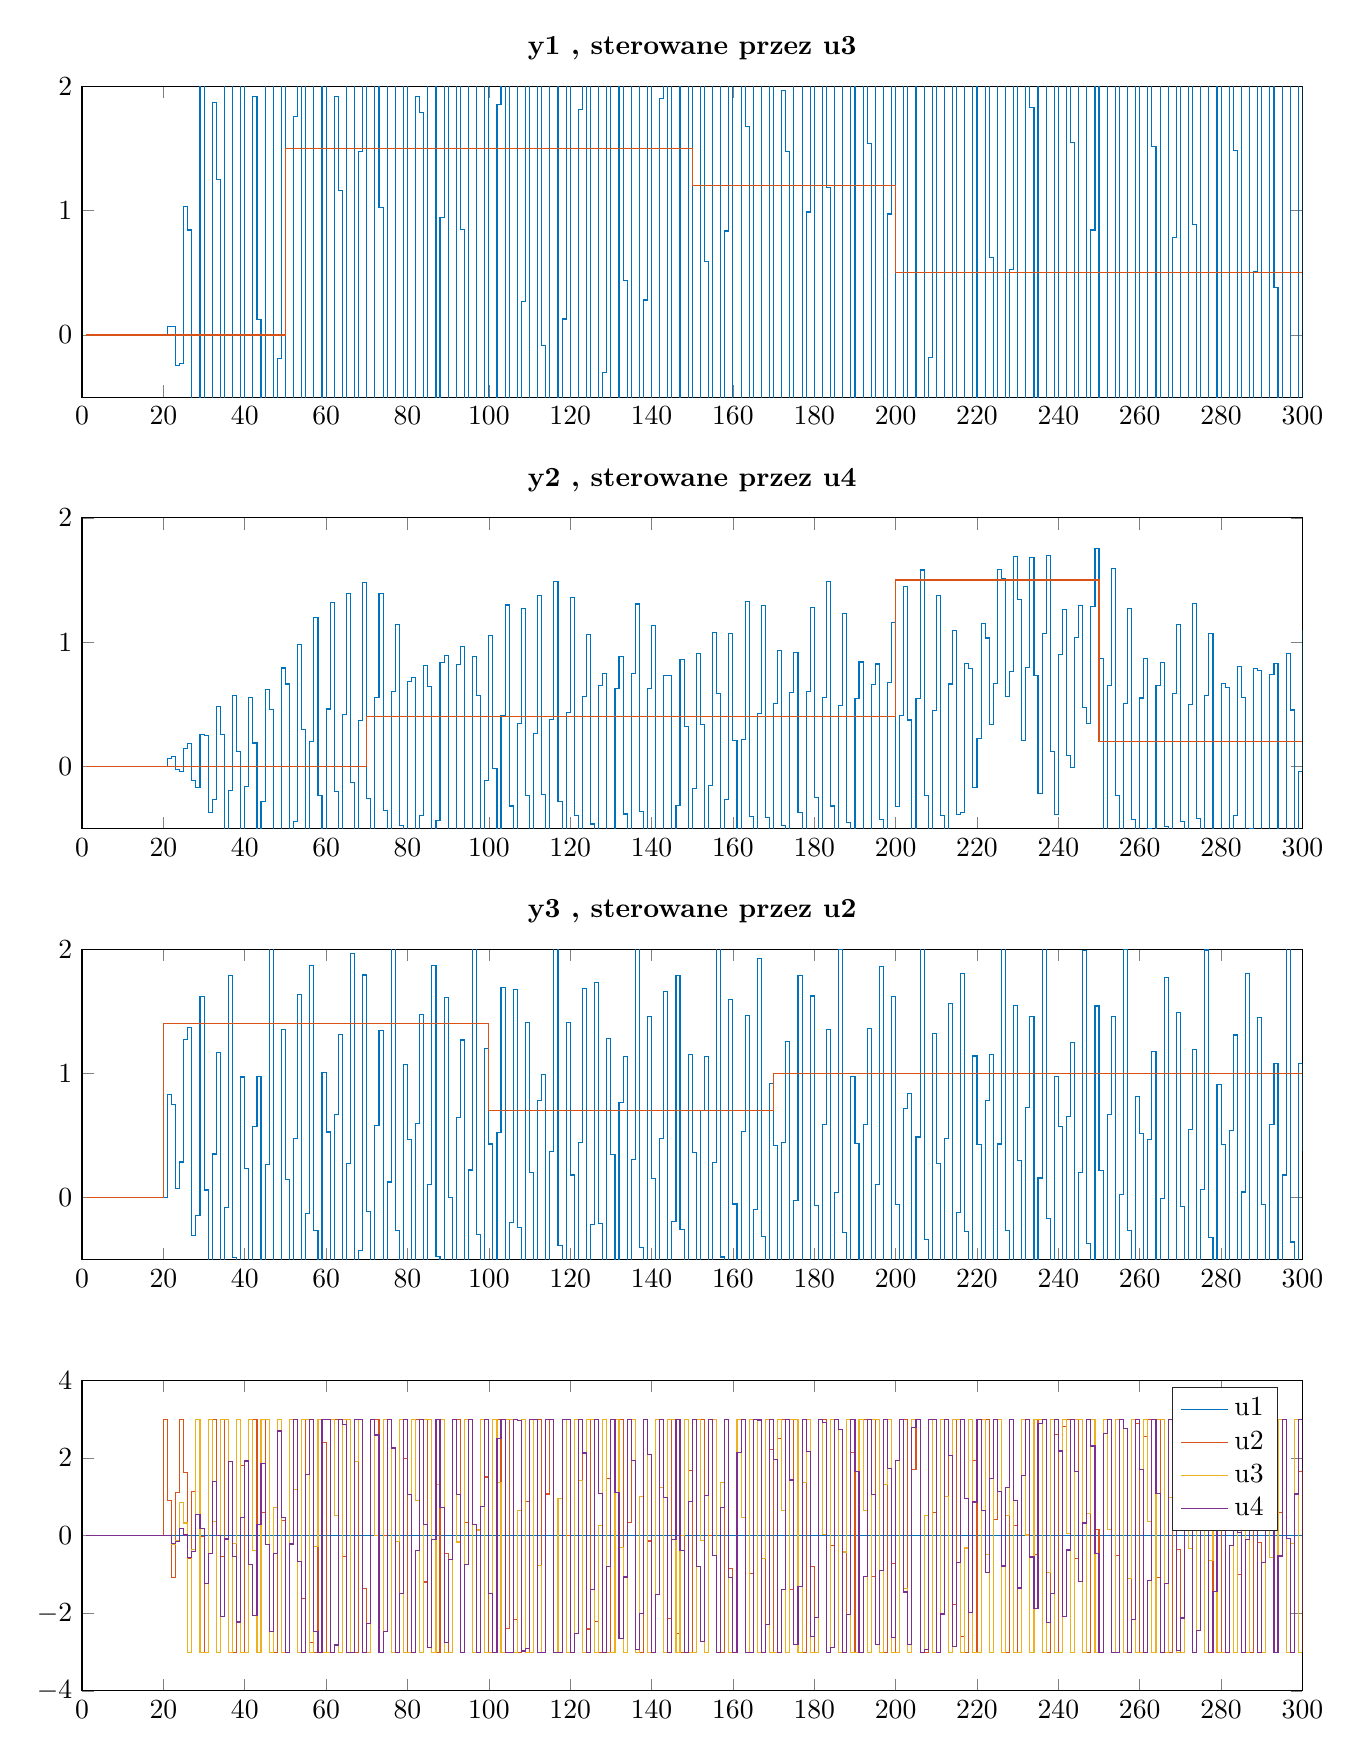
\begin{tikzpicture}

\begin{axis}[%
width=6.102in,
height=1.553in,
at={(1.024in,7.552in)},
scale only axis,
xmin=0,
xmax=300,
ymin=-0.5,
ymax=2,
axis background/.style={fill=white},
title style={font=\bfseries},
title={y1 , sterowane przez u3}
]
\addplot[const plot, color=mycolor1, forget plot] table[row sep=crcr] {%
1	0\\
2	0\\
3	0\\
4	0\\
5	0\\
6	0\\
7	0\\
8	0\\
9	0\\
10	0\\
11	0\\
12	0\\
13	0\\
14	0\\
15	0\\
16	0\\
17	0\\
18	0\\
19	0\\
20	0\\
21	0.0663597650785785\\
22	0.071588966531205\\
23	-0.242951077916027\\
24	-0.233231331265886\\
25	1.03617359328443\\
26	0.844543912000835\\
27	-3.3083187371695\\
28	-1.6514491685918\\
29	3.09152612007136\\
30	-2.41774383850017\\
31	-4.62468002964849\\
32	1.87071941813116\\
33	1.24813232676415\\
34	-3.17454307150153\\
35	2.25659710797501\\
36	4.3896827290008\\
37	-1.97795689566018\\
38	-1.09153251616683\\
39	3.02612770353695\\
40	-2.54351550968753\\
41	-4.53967149242059\\
42	1.91646975827085\\
43	0.125040859598633\\
44	-3.69602728142241\\
45	2.2932278731818\\
46	4.48052983741214\\
47	-2.21457586703789\\
48	-0.191308115656096\\
49	3.62945305943156\\
50	-2.24110552370623\\
51	-4.72375010847698\\
52	1.75705331898455\\
53	2.26078745183512\\
54	-2.84887883985857\\
55	2.2585871946253\\
56	4.45156932536294\\
57	-1.85189058555632\\
58	-1.24272817658569\\
59	2.8860417500033\\
60	-2.43848982658444\\
61	-4.34822807132632\\
62	1.92110274903777\\
63	1.16012450113371\\
64	-3.13122591795402\\
65	2.64865880498628\\
66	4.51549811828574\\
67	-2.25082013394901\\
68	1.47326296427841\\
69	4.39452551224985\\
70	-2.135186197045\\
71	-4.67047604708211\\
72	2.02510612722409\\
73	1.02834008927755\\
74	-3.36893410375518\\
75	2.15091788374228\\
76	4.56985787075654\\
77	-1.76699522957916\\
78	-1.01811815719508\\
79	3.12062048902754\\
80	-2.26211767394639\\
81	-4.34780543327898\\
82	1.9174397080289\\
83	1.78792742955823\\
84	-2.79381047693235\\
85	2.65502094266029\\
86	4.49977781581111\\
87	-2.04781440943917\\
88	0.94807679778572\\
89	4.12844283000328\\
90	-2.19604162156129\\
91	-4.54584303166294\\
92	2.16048563046841\\
93	0.846940226518881\\
94	-3.42659240843622\\
95	2.28075407292446\\
96	4.70538280628877\\
97	-1.7914302923384\\
98	-0.689915762745582\\
99	3.40633924375992\\
100	-2.07851608111904\\
101	-4.40188060364628\\
102	1.85764658941248\\
103	2.52810639090326\\
104	-2.42627892419163\\
105	2.59507988272838\\
106	4.39368778537524\\
107	-1.89740105338882\\
108	0.268977978095923\\
109	3.66065523042863\\
110	-2.44776022211995\\
111	-4.43953298953407\\
112	2.27955647404546\\
113	-0.0834301819531591\\
114	-3.88406745892377\\
115	2.31531568424309\\
116	4.79052261798732\\
117	-1.95168506846713\\
118	0.128500933885368\\
119	3.80207631467612\\
120	-1.94291342998195\\
121	-4.46292459752629\\
122	1.81392632572063\\
123	2.58058921500453\\
124	-2.48251490316927\\
125	2.52909591909592\\
126	4.45407670719041\\
127	-1.84258404400937\\
128	-0.304030945635337\\
129	3.39333311387811\\
130	-2.41804663564476\\
131	-4.37649716872476\\
132	2.20138937571975\\
133	0.439861856768619\\
134	-3.56240292115703\\
135	2.48253431766332\\
136	4.82182898038736\\
137	-1.93075137451506\\
138	0.281603746995907\\
139	3.91093932700411\\
140	-1.92757025865952\\
141	-4.45223540583576\\
142	1.90230479140883\\
143	2.4479586846121\\
144	-2.57410889420992\\
145	2.49484402880307\\
146	4.54040311223914\\
147	-1.76314106998394\\
148	-0.654199872268486\\
149	3.24432758135218\\
150	-2.35559427294851\\
151	-4.29387739872207\\
152	2.13739003743474\\
153	0.588101461760115\\
154	-3.37810905475128\\
155	2.60416102957395\\
156	4.72825305074388\\
157	-2.02967476691316\\
158	0.836915257457381\\
159	4.18296099495462\\
160	-2.02860961853312\\
161	-4.57819539652949\\
162	2.06224646845969\\
163	1.67701515081177\\
164	-3.08707349016682\\
165	2.23185073724027\\
166	4.60459354652141\\
167	-1.69144169633022\\
168	-1.48243936411293\\
169	2.924782181987\\
170	-2.32918756094238\\
171	-4.29870077799369\\
172	1.96752334770641\\
173	1.4794622693851\\
174	-2.91782111058568\\
175	2.6862148109549\\
176	4.55881836018802\\
177	-2.077378230517\\
178	0.989491606130157\\
179	4.24637568471641\\
180	-2.09312944689572\\
181	-4.57000465009585\\
182	2.13724361396818\\
183	1.18867348157953\\
184	-3.22962679451526\\
185	2.24038556970806\\
186	4.65315272738239\\
187	-1.65139051438053\\
188	-1.23878141780873\\
189	3.06086633546246\\
190	-2.24544552698102\\
191	-4.25952305857766\\
192	2.00949658996083\\
193	1.53968092995618\\
194	-2.86238041891585\\
195	2.71569312272815\\
196	4.58439757498418\\
197	-2.02399208191067\\
198	0.973500778174566\\
199	4.2318934175219\\
200	-2.09427727320075\\
201	-4.24721506180929\\
202	2.44166106577015\\
203	-0.521158666498983\\
204	-3.87694453911656\\
205	2.46925015414214\\
206	4.98869761552256\\
207	-1.74609040548857\\
208	-0.178385153592412\\
209	3.80935417652063\\
210	-1.81474270691262\\
211	-4.30471454933537\\
212	2.01507015830823\\
213	2.26926220602669\\
214	-2.49065322593467\\
215	2.65275654579321\\
216	4.66184649654564\\
217	-1.64408155221159\\
218	-0.809761655980712\\
219	3.39196664919758\\
220	-2.13449433670413\\
221	-4.05849767176265\\
222	2.48315163795132\\
223	0.624403781178314\\
224	-3.0616616148825\\
225	3.0014710762539\\
226	5.26276052785078\\
227	-1.34193908652747\\
228	0.527536799349917\\
229	4.46479167940406\\
230	-1.37383951404099\\
231	-3.7598599277061\\
232	2.80927443119867\\
233	1.83040654777236\\
234	-2.43051964719933\\
235	3.06409453702974\\
236	5.41729050495838\\
237	-0.912637899428308\\
238	-1.10840410089534\\
239	3.58140229034821\\
240	-1.61572427683012\\
241	-3.58028281755954\\
242	2.73269595642517\\
243	1.54880720250739\\
244	-2.43481105727762\\
245	3.32758520669801\\
246	5.3416640742011\\
247	-1.19634160227147\\
248	0.845060897185689\\
249	4.68095365942063\\
250	-1.28974303449194\\
251	-3.81360856174872\\
252	2.84277794886159\\
253	2.03244272036229\\
254	-2.53047487956357\\
255	2.84649518041785\\
256	5.2097551241592\\
257	-1.13093389916639\\
258	-1.56637164172009\\
259	3.20634506782732\\
260	-1.9216898675241\\
261	-3.89215195279246\\
262	2.36585590141298\\
263	1.5169979236335\\
264	-2.67669796890734\\
265	2.96818199091288\\
266	4.83381162459329\\
267	-1.80542919155638\\
268	0.783120029638868\\
269	4.2895360966087\\
270	-1.97306656669623\\
271	-4.42394063547989\\
272	2.28609547660063\\
273	0.891857577754921\\
274	-3.27377295995698\\
275	2.32803892397969\\
276	4.76528767957492\\
277	-1.58310533645105\\
278	-1.42356025807498\\
279	3.0779840867765\\
280	-2.17262659900076\\
281	-4.23343947786288\\
282	2.04028495724923\\
283	1.48448731787363\\
284	-2.82932232661122\\
285	2.70116387291076\\
286	4.56597489567433\\
287	-1.97314088058707\\
288	0.511775600078267\\
289	3.99428791726818\\
290	-2.22755138703489\\
291	-4.54274680109694\\
292	2.17699285236981\\
293	0.379849709713887\\
294	-3.59533301847776\\
295	2.24513021671526\\
296	4.70723439268088\\
297	-1.80482473017176\\
298	-1.10398494952245\\
299	3.27516391825184\\
300	-2.11299071012907\\
};
\addplot[const plot, color=mycolor2, forget plot] table[row sep=crcr] {%
1	0\\
2	0\\
3	0\\
4	0\\
5	0\\
6	0\\
7	0\\
8	0\\
9	0\\
10	0\\
11	0\\
12	0\\
13	0\\
14	0\\
15	0\\
16	0\\
17	0\\
18	0\\
19	0\\
20	0\\
21	0\\
22	0\\
23	0\\
24	0\\
25	0\\
26	0\\
27	0\\
28	0\\
29	0\\
30	0\\
31	0\\
32	0\\
33	0\\
34	0\\
35	0\\
36	0\\
37	0\\
38	0\\
39	0\\
40	0\\
41	0\\
42	0\\
43	0\\
44	0\\
45	0\\
46	0\\
47	0\\
48	0\\
49	0\\
50	1.5\\
51	1.5\\
52	1.5\\
53	1.5\\
54	1.5\\
55	1.5\\
56	1.5\\
57	1.5\\
58	1.5\\
59	1.5\\
60	1.5\\
61	1.5\\
62	1.5\\
63	1.5\\
64	1.5\\
65	1.5\\
66	1.5\\
67	1.5\\
68	1.5\\
69	1.5\\
70	1.5\\
71	1.5\\
72	1.5\\
73	1.5\\
74	1.5\\
75	1.5\\
76	1.5\\
77	1.5\\
78	1.5\\
79	1.5\\
80	1.5\\
81	1.5\\
82	1.5\\
83	1.5\\
84	1.5\\
85	1.5\\
86	1.5\\
87	1.5\\
88	1.5\\
89	1.5\\
90	1.5\\
91	1.5\\
92	1.5\\
93	1.5\\
94	1.5\\
95	1.5\\
96	1.5\\
97	1.5\\
98	1.5\\
99	1.5\\
100	1.5\\
101	1.5\\
102	1.5\\
103	1.5\\
104	1.5\\
105	1.5\\
106	1.5\\
107	1.5\\
108	1.5\\
109	1.5\\
110	1.5\\
111	1.5\\
112	1.5\\
113	1.5\\
114	1.5\\
115	1.5\\
116	1.5\\
117	1.5\\
118	1.5\\
119	1.5\\
120	1.5\\
121	1.5\\
122	1.5\\
123	1.5\\
124	1.5\\
125	1.5\\
126	1.5\\
127	1.5\\
128	1.5\\
129	1.5\\
130	1.5\\
131	1.5\\
132	1.5\\
133	1.5\\
134	1.5\\
135	1.5\\
136	1.5\\
137	1.5\\
138	1.5\\
139	1.5\\
140	1.5\\
141	1.5\\
142	1.5\\
143	1.5\\
144	1.5\\
145	1.5\\
146	1.5\\
147	1.5\\
148	1.5\\
149	1.5\\
150	1.2\\
151	1.2\\
152	1.2\\
153	1.2\\
154	1.2\\
155	1.2\\
156	1.2\\
157	1.2\\
158	1.2\\
159	1.2\\
160	1.2\\
161	1.2\\
162	1.2\\
163	1.2\\
164	1.2\\
165	1.2\\
166	1.2\\
167	1.2\\
168	1.2\\
169	1.2\\
170	1.2\\
171	1.2\\
172	1.2\\
173	1.2\\
174	1.2\\
175	1.2\\
176	1.2\\
177	1.2\\
178	1.2\\
179	1.2\\
180	1.2\\
181	1.2\\
182	1.2\\
183	1.2\\
184	1.2\\
185	1.2\\
186	1.2\\
187	1.2\\
188	1.2\\
189	1.2\\
190	1.2\\
191	1.2\\
192	1.2\\
193	1.2\\
194	1.2\\
195	1.2\\
196	1.2\\
197	1.2\\
198	1.2\\
199	1.2\\
200	0.5\\
201	0.5\\
202	0.5\\
203	0.5\\
204	0.5\\
205	0.5\\
206	0.5\\
207	0.5\\
208	0.5\\
209	0.5\\
210	0.5\\
211	0.5\\
212	0.5\\
213	0.5\\
214	0.5\\
215	0.5\\
216	0.5\\
217	0.5\\
218	0.5\\
219	0.5\\
220	0.5\\
221	0.5\\
222	0.5\\
223	0.5\\
224	0.5\\
225	0.5\\
226	0.5\\
227	0.5\\
228	0.5\\
229	0.5\\
230	0.5\\
231	0.5\\
232	0.5\\
233	0.5\\
234	0.5\\
235	0.5\\
236	0.5\\
237	0.5\\
238	0.5\\
239	0.5\\
240	0.5\\
241	0.5\\
242	0.5\\
243	0.5\\
244	0.5\\
245	0.5\\
246	0.5\\
247	0.5\\
248	0.5\\
249	0.5\\
250	0.5\\
251	0.5\\
252	0.5\\
253	0.5\\
254	0.5\\
255	0.5\\
256	0.5\\
257	0.5\\
258	0.5\\
259	0.5\\
260	0.5\\
261	0.5\\
262	0.5\\
263	0.5\\
264	0.5\\
265	0.5\\
266	0.5\\
267	0.5\\
268	0.5\\
269	0.5\\
270	0.5\\
271	0.5\\
272	0.5\\
273	0.5\\
274	0.5\\
275	0.5\\
276	0.5\\
277	0.5\\
278	0.5\\
279	0.5\\
280	0.5\\
281	0.5\\
282	0.5\\
283	0.5\\
284	0.5\\
285	0.5\\
286	0.5\\
287	0.5\\
288	0.5\\
289	0.5\\
290	0.5\\
291	0.5\\
292	0.5\\
293	0.5\\
294	0.5\\
295	0.5\\
296	0.5\\
297	0.5\\
298	0.5\\
299	0.5\\
300	0.5\\
};
\end{axis}

\begin{axis}[%
width=6.102in,
height=1.553in,
at={(1.024in,5.395in)},
scale only axis,
xmin=0,
xmax=300,
ymin=-0.5,
ymax=2,
axis background/.style={fill=white},
title style={font=\bfseries},
title={y2 , sterowane przez u4}
]
\addplot[const plot, color=mycolor1, forget plot] table[row sep=crcr] {%
1	0\\
2	0\\
3	0\\
4	0\\
5	0\\
6	0\\
7	0\\
8	0\\
9	0\\
10	0\\
11	0\\
12	0\\
13	0\\
14	0\\
15	0\\
16	0\\
17	0\\
18	0\\
19	0\\
20	0\\
21	0.0612158143362928\\
22	0.0770823080206103\\
23	-0.026683860148535\\
24	-0.0384503650416268\\
25	0.142135808901131\\
26	0.180863933542452\\
27	-0.113999874825863\\
28	-0.1697642816758\\
29	0.256984228307289\\
30	0.246420722134851\\
31	-0.369974870706902\\
32	-0.263711823243118\\
33	0.484826398578853\\
34	0.253401538790168\\
35	-0.544624736536162\\
36	-0.193569401409182\\
37	0.568538691509165\\
38	0.119842679254607\\
39	-0.620525392026487\\
40	-0.161679388247324\\
41	0.553145549386055\\
42	0.187984388652194\\
43	-0.553598633233915\\
44	-0.283521719508793\\
45	0.619657355283611\\
46	0.458783485539679\\
47	-0.680954014155839\\
48	-0.589445296125996\\
49	0.791397228003688\\
50	0.663017584507726\\
51	-0.794530399928345\\
52	-0.441922371163652\\
53	0.979549354526797\\
54	0.296490012280152\\
55	-0.890646983876766\\
56	0.19788835908448\\
57	1.19678279875194\\
58	-0.235223164417573\\
59	-1.14268396586557\\
60	0.461448622027073\\
61	1.32180424286032\\
62	-0.202749817860451\\
63	-1.06713321761167\\
64	0.416917179714243\\
65	1.38851903850899\\
66	-0.128072552647437\\
67	-1.24758267578028\\
68	0.367109755706619\\
69	1.47752433762953\\
70	-0.257574699211229\\
71	-1.09854976027292\\
72	0.555262926818642\\
73	1.38843298326534\\
74	-0.355708314253852\\
75	-1.08368198213754\\
76	0.601017004173676\\
77	1.14531117740465\\
78	-0.476996532721604\\
79	-0.741253221215913\\
80	0.684683042621557\\
81	0.714736813244216\\
82	-0.585000244445401\\
83	-0.397017516193357\\
84	0.812422957328951\\
85	0.639956990978321\\
86	-0.550209130270101\\
87	-0.434638388574782\\
88	0.834697614775669\\
89	0.891476591544026\\
90	-0.520485870173549\\
91	-0.653317074188913\\
92	0.816641413549806\\
93	0.966066876198649\\
94	-0.620661202338616\\
95	-0.601692521856565\\
96	0.887827740235996\\
97	0.573836990967679\\
98	-0.822995144600925\\
99	-0.110960302737385\\
100	1.05412614838385\\
101	-0.0203109664985\\
102	-1.03691566272903\\
103	0.409809431813449\\
104	1.29885518928485\\
105	-0.319110142475324\\
106	-1.1905367047686\\
107	0.342047439032696\\
108	1.27155948622807\\
109	-0.232149763574405\\
110	-1.23600881903161\\
111	0.268049226003157\\
112	1.37735839538761\\
113	-0.224091902019827\\
114	-1.34408706295961\\
115	0.376607154087585\\
116	1.48555185300869\\
117	-0.28350632672148\\
118	-1.32333501654647\\
119	0.433456152783157\\
120	1.36228276126203\\
121	-0.398206257898537\\
122	-1.09006718015998\\
123	0.564654362591728\\
124	1.06401805466917\\
125	-0.464242980461789\\
126	-0.681331644325923\\
127	0.647634284864396\\
128	0.74598141563445\\
129	-0.565960970985835\\
130	-0.640324673765703\\
131	0.629460215822597\\
132	0.886813760856969\\
133	-0.383324933549148\\
134	-0.714862470541487\\
135	0.746143810613611\\
136	1.30659956564887\\
137	-0.366701387500287\\
138	-1.00079636593662\\
139	0.626766541340927\\
140	1.13677882739564\\
141	-0.538355729595264\\
142	-0.802318164102222\\
143	0.732546687542955\\
144	0.731870594266744\\
145	-0.664038394343193\\
146	-0.317846165123875\\
147	0.859660397489259\\
148	0.317604175951704\\
149	-0.831110737932688\\
150	-0.177107251088307\\
151	0.907063776151313\\
152	0.338780752884274\\
153	-0.745149533284634\\
154	-0.153553364263577\\
155	1.07811435913359\\
156	0.589299948630255\\
157	-0.833651016444589\\
158	-0.267635494634781\\
159	1.06995696074904\\
160	0.206167875085657\\
161	-1.1094520505034\\
162	0.214154195104873\\
163	1.32822267043685\\
164	-0.403793498165607\\
165	-1.33928568899777\\
166	0.428205568941831\\
167	1.29357673081572\\
168	-0.411875590089786\\
169	-1.01586521922\\
170	0.505344330034289\\
171	0.929418068240457\\
172	-0.479225862218536\\
173	-0.728443299324447\\
174	0.59368944225519\\
175	0.916272723837651\\
176	-0.371954438736835\\
177	-0.79130187446589\\
178	0.603554642934214\\
179	1.27969942312581\\
180	-0.248343611499367\\
181	-1.06199574902099\\
182	0.553634540629251\\
183	1.48498268552929\\
184	-0.318712628758924\\
185	-1.23487774669959\\
186	0.487691059995496\\
187	1.23309670283957\\
188	-0.448726916616695\\
189	-0.939376711995344\\
190	0.548076748618649\\
191	0.839654916275897\\
192	-0.525885195374677\\
193	-0.62775293326984\\
194	0.655995316515675\\
195	0.824151388441341\\
196	-0.424312856564176\\
197	-0.672418487303605\\
198	0.677968675622958\\
199	1.15921467991405\\
200	-0.325979669644582\\
201	0.411338222751198\\
202	1.45032655057202\\
203	0.373591106590633\\
204	-0.927271689102007\\
205	0.548965296534267\\
206	1.58014646797065\\
207	-0.23552956589748\\
208	-1.28259809166116\\
209	0.447332820356939\\
210	1.37229171177903\\
211	-0.397517082757156\\
212	-0.907004593956208\\
213	0.663105819393404\\
214	1.09404230409896\\
215	-0.384565942720936\\
216	-0.372226172639006\\
217	0.826075405879614\\
218	0.788942941247228\\
219	-0.168300701963406\\
220	0.221367012448892\\
221	1.1500730925143\\
222	1.03362825566307\\
223	0.33939140020435\\
224	0.667298657512834\\
225	1.58433462305316\\
226	1.51405165538129\\
227	0.559535501344207\\
228	0.76119807981634\\
229	1.69259910034117\\
230	1.34333503420029\\
231	0.204995128665996\\
232	0.796655450265923\\
233	1.6801680401957\\
234	0.729498417688219\\
235	-0.221108239062527\\
236	1.06965430011865\\
237	1.69954201421812\\
238	0.122085581925454\\
239	-0.384291518839473\\
240	0.902734808814683\\
241	1.26277197353604\\
242	0.0849406054361235\\
243	-0.00609858116062623\\
244	1.03958191591602\\
245	1.29145089254717\\
246	0.474476531537436\\
247	0.342212572764524\\
248	1.28875100601851\\
249	1.75451189061872\\
250	0.871088422412133\\
251	-0.699142042101258\\
252	0.648739192694379\\
253	1.59283023948025\\
254	-0.237984795522994\\
255	-1.22360599848567\\
256	0.507348418566562\\
257	1.26916287843776\\
258	-0.427573165580637\\
259	-0.97325382189121\\
260	0.550522152588307\\
261	0.868830830046723\\
262	-0.50413774405808\\
263	-0.653741909179747\\
264	0.648027168218216\\
265	0.837749647797228\\
266	-0.483526933701142\\
267	-0.82446842623051\\
268	0.5869129917497\\
269	1.1415339670093\\
270	-0.444250101457582\\
271	-1.17285431481556\\
272	0.497563181365174\\
273	1.30818333111295\\
274	-0.417170870472813\\
275	-1.11654913496142\\
276	0.571123985440957\\
277	1.07135972538172\\
278	-0.539635270226135\\
279	-0.766000575722217\\
280	0.666460664558334\\
281	0.633654867971462\\
282	-0.640369799333014\\
283	-0.39586308784922\\
284	0.805906695083751\\
285	0.556749919895266\\
286	-0.652385577653694\\
287	-0.496577525758575\\
288	0.785283089974582\\
289	0.77437199667586\\
290	-0.681680178727411\\
291	-0.780912337340978\\
292	0.73692818659171\\
293	0.827261438861179\\
294	-0.708740571735308\\
295	-0.568005139399835\\
296	0.907199815564838\\
297	0.45391544435423\\
298	-0.902635802838996\\
299	-0.0439032102548567\\
300	1.0960555332901\\
};
\addplot[const plot, color=mycolor2, forget plot] table[row sep=crcr] {%
1	0\\
2	0\\
3	0\\
4	0\\
5	0\\
6	0\\
7	0\\
8	0\\
9	0\\
10	0\\
11	0\\
12	0\\
13	0\\
14	0\\
15	0\\
16	0\\
17	0\\
18	0\\
19	0\\
20	0\\
21	0\\
22	0\\
23	0\\
24	0\\
25	0\\
26	0\\
27	0\\
28	0\\
29	0\\
30	0\\
31	0\\
32	0\\
33	0\\
34	0\\
35	0\\
36	0\\
37	0\\
38	0\\
39	0\\
40	0\\
41	0\\
42	0\\
43	0\\
44	0\\
45	0\\
46	0\\
47	0\\
48	0\\
49	0\\
50	0\\
51	0\\
52	0\\
53	0\\
54	0\\
55	0\\
56	0\\
57	0\\
58	0\\
59	0\\
60	0\\
61	0\\
62	0\\
63	0\\
64	0\\
65	0\\
66	0\\
67	0\\
68	0\\
69	0\\
70	0.4\\
71	0.4\\
72	0.4\\
73	0.4\\
74	0.4\\
75	0.4\\
76	0.4\\
77	0.4\\
78	0.4\\
79	0.4\\
80	0.4\\
81	0.4\\
82	0.4\\
83	0.4\\
84	0.4\\
85	0.4\\
86	0.4\\
87	0.4\\
88	0.4\\
89	0.4\\
90	0.4\\
91	0.4\\
92	0.4\\
93	0.4\\
94	0.4\\
95	0.4\\
96	0.4\\
97	0.4\\
98	0.4\\
99	0.4\\
100	0.4\\
101	0.4\\
102	0.4\\
103	0.4\\
104	0.4\\
105	0.4\\
106	0.4\\
107	0.4\\
108	0.4\\
109	0.4\\
110	0.4\\
111	0.4\\
112	0.4\\
113	0.4\\
114	0.4\\
115	0.4\\
116	0.4\\
117	0.4\\
118	0.4\\
119	0.4\\
120	0.4\\
121	0.4\\
122	0.4\\
123	0.4\\
124	0.4\\
125	0.4\\
126	0.4\\
127	0.4\\
128	0.4\\
129	0.4\\
130	0.4\\
131	0.4\\
132	0.4\\
133	0.4\\
134	0.4\\
135	0.4\\
136	0.4\\
137	0.4\\
138	0.4\\
139	0.4\\
140	0.4\\
141	0.4\\
142	0.4\\
143	0.4\\
144	0.4\\
145	0.4\\
146	0.4\\
147	0.4\\
148	0.4\\
149	0.4\\
150	0.4\\
151	0.4\\
152	0.4\\
153	0.4\\
154	0.4\\
155	0.4\\
156	0.4\\
157	0.4\\
158	0.4\\
159	0.4\\
160	0.4\\
161	0.4\\
162	0.4\\
163	0.4\\
164	0.4\\
165	0.4\\
166	0.4\\
167	0.4\\
168	0.4\\
169	0.4\\
170	0.4\\
171	0.4\\
172	0.4\\
173	0.4\\
174	0.4\\
175	0.4\\
176	0.4\\
177	0.4\\
178	0.4\\
179	0.4\\
180	0.4\\
181	0.4\\
182	0.4\\
183	0.4\\
184	0.4\\
185	0.4\\
186	0.4\\
187	0.4\\
188	0.4\\
189	0.4\\
190	0.4\\
191	0.4\\
192	0.4\\
193	0.4\\
194	0.4\\
195	0.4\\
196	0.4\\
197	0.4\\
198	0.4\\
199	0.4\\
200	1.5\\
201	1.5\\
202	1.5\\
203	1.5\\
204	1.5\\
205	1.5\\
206	1.5\\
207	1.5\\
208	1.5\\
209	1.5\\
210	1.5\\
211	1.5\\
212	1.5\\
213	1.5\\
214	1.5\\
215	1.5\\
216	1.5\\
217	1.5\\
218	1.5\\
219	1.5\\
220	1.5\\
221	1.5\\
222	1.5\\
223	1.5\\
224	1.5\\
225	1.5\\
226	1.5\\
227	1.5\\
228	1.5\\
229	1.5\\
230	1.5\\
231	1.5\\
232	1.5\\
233	1.5\\
234	1.5\\
235	1.5\\
236	1.5\\
237	1.5\\
238	1.5\\
239	1.5\\
240	1.5\\
241	1.5\\
242	1.5\\
243	1.5\\
244	1.5\\
245	1.5\\
246	1.5\\
247	1.5\\
248	1.5\\
249	1.5\\
250	0.2\\
251	0.2\\
252	0.2\\
253	0.2\\
254	0.2\\
255	0.2\\
256	0.2\\
257	0.2\\
258	0.2\\
259	0.2\\
260	0.2\\
261	0.2\\
262	0.2\\
263	0.2\\
264	0.2\\
265	0.2\\
266	0.2\\
267	0.2\\
268	0.2\\
269	0.2\\
270	0.2\\
271	0.2\\
272	0.2\\
273	0.2\\
274	0.2\\
275	0.2\\
276	0.2\\
277	0.2\\
278	0.2\\
279	0.2\\
280	0.2\\
281	0.2\\
282	0.2\\
283	0.2\\
284	0.2\\
285	0.2\\
286	0.2\\
287	0.2\\
288	0.2\\
289	0.2\\
290	0.2\\
291	0.2\\
292	0.2\\
293	0.2\\
294	0.2\\
295	0.2\\
296	0.2\\
297	0.2\\
298	0.2\\
299	0.2\\
300	0.2\\
};
\end{axis}

\begin{axis}[%
width=6.102in,
height=1.553in,
at={(1.024in,3.239in)},
scale only axis,
xmin=0,
xmax=300,
ymin=-0.5,
ymax=2,
axis background/.style={fill=white},
title style={font=\bfseries},
title={y3 , sterowane przez u2}
]
\addplot[const plot, color=mycolor1, forget plot] table[row sep=crcr] {%
1	0\\
2	0\\
3	0\\
4	0\\
5	0\\
6	0\\
7	0\\
8	0\\
9	0\\
10	0\\
11	0\\
12	0\\
13	0\\
14	0\\
15	0\\
16	0\\
17	0\\
18	0\\
19	0\\
20	0\\
21	0.82628561460347\\
22	0.749053243317543\\
23	0.0761713741540198\\
24	0.286129511151675\\
25	1.27280694688117\\
26	1.365298295374\\
27	-0.30766512039124\\
28	-0.147680606674946\\
29	1.61817626642654\\
30	0.0608767189025933\\
31	-1.94658657931344\\
32	0.35083692468693\\
33	1.16717178496895\\
34	-1.11690340518574\\
35	-0.0831572887989673\\
36	1.78479641362402\\
37	-0.483023058281706\\
38	-1.21894081936476\\
39	0.970815309817139\\
40	0.237170330760582\\
41	-1.67110003738013\\
42	0.572737790950721\\
43	0.972167274868663\\
44	-1.25938555053161\\
45	0.269197112011858\\
46	2.00829495284137\\
47	-0.504091801494609\\
48	-0.952308253154745\\
49	1.34996920551574\\
50	0.143459306894402\\
51	-1.86348159329455\\
52	0.473971731106342\\
53	1.63167300293966\\
54	-0.758564989552392\\
55	-0.127046195316588\\
56	1.87142331713526\\
57	-0.267567639529058\\
58	-1.14041830858187\\
59	1.0077912304962\\
60	0.528081682401007\\
61	-1.42462604090123\\
62	0.668828903701644\\
63	1.30915654646329\\
64	-0.900315237323037\\
65	0.277272018416136\\
66	1.96663012552367\\
67	-0.526589118353775\\
68	-0.424058885339943\\
69	1.79150373265471\\
70	-0.111124950307566\\
71	-1.95000516874091\\
72	0.581779157146867\\
73	1.34126406705846\\
74	-1.0496737811996\\
75	0.125154245571224\\
76	2.05249133859377\\
77	-0.261786772410326\\
78	-1.12140335245699\\
79	1.07126863016798\\
80	0.46673658869196\\
81	-1.52841687056732\\
82	0.595027189678813\\
83	1.47048093426809\\
84	-0.766636443586439\\
85	0.104562149231778\\
86	1.86645756699259\\
87	-0.475943846293736\\
88	-0.564085309088923\\
89	1.60678506477225\\
90	0.00345804639305047\\
91	-1.83870083988027\\
92	0.647612270657564\\
93	1.26846184776692\\
94	-1.11685215082176\\
95	0.222237728003159\\
96	2.11266378162712\\
97	-0.29948873441492\\
98	-1.06367941287571\\
99	1.19627487668581\\
100	0.431293628770049\\
101	-1.62899285114141\\
102	0.52594258374526\\
103	1.69009244616564\\
104	-0.586050901771461\\
105	-0.201794860966372\\
106	1.67617464757664\\
107	-0.242565678436625\\
108	-0.622397499333783\\
109	1.41180877705982\\
110	0.19855338564391\\
111	-1.62104209419645\\
112	0.780642739805818\\
113	0.993895590445023\\
114	-1.35318768489515\\
115	0.370324606885093\\
116	2.19178645076673\\
117	-0.384482930299681\\
118	-0.883938377086588\\
119	1.40879015496276\\
120	0.181209605774988\\
121	-1.81214026158921\\
122	0.440205403144428\\
123	1.6836569848411\\
124	-0.608905517206818\\
125	-0.217736209047073\\
126	1.73032644261568\\
127	-0.205640000871276\\
128	-0.790459370816712\\
129	1.27979245265002\\
130	0.344999220808764\\
131	-1.53166396663507\\
132	0.763215978678896\\
133	1.13701467246144\\
134	-1.17497630781154\\
135	0.309174387265025\\
136	2.13861826247369\\
137	-0.403410372669644\\
138	-0.831771490101827\\
139	1.45942901648691\\
140	0.150592414328459\\
141	-1.82639373766872\\
142	0.473457869296632\\
143	1.65599966328646\\
144	-0.670345636070976\\
145	-0.189408535450262\\
146	1.78895905682405\\
147	-0.2554733592115\\
148	-0.958672797838432\\
149	1.15345897698269\\
150	0.366219925757007\\
151	-1.5189304531543\\
152	0.698289144964235\\
153	1.13648477712825\\
154	-1.09918593508019\\
155	0.279004316255903\\
156	2.03912511023546\\
157	-0.478616246387429\\
158	-0.663828174897459\\
159	1.59757737770045\\
160	-0.0518412567431205\\
161	-1.95478146787975\\
162	0.530525146997563\\
163	1.46515139932062\\
164	-0.959085785215272\\
165	-0.0996470215206953\\
166	1.92068068039231\\
167	-0.310796638018428\\
168	-1.28898067572641\\
169	0.921088983542712\\
170	0.416488692523497\\
171	-1.54104531522843\\
172	0.444416702818066\\
173	1.25860707137248\\
174	-0.920456913155443\\
175	-0.0202123842801796\\
176	1.7882640522912\\
177	-0.572464260481289\\
178	-0.617633662608771\\
179	1.62264392282375\\
180	-0.0641203838410136\\
181	-1.92928383582241\\
182	0.585535468464611\\
183	1.35585709224425\\
184	-1.04146865871773\\
185	0.0403103744125581\\
186	1.99778013044012\\
187	-0.279214168949669\\
188	-1.22045374268378\\
189	0.977855592414912\\
190	0.436120485177351\\
191	-1.53550701365867\\
192	0.587150372520554\\
193	1.3589303866652\\
194	-0.855610110189564\\
195	0.102159841044716\\
196	1.86185936335638\\
197	-0.513270948495958\\
198	-0.59651324473782\\
199	1.61769843071123\\
200	-0.0543579608600198\\
201	-1.77131641217535\\
202	0.715682705314755\\
203	0.839973797442725\\
204	-1.44121274988768\\
205	0.487721298028678\\
206	2.26409884260934\\
207	-0.338592602426556\\
208	-0.992312319293616\\
209	1.3221883553333\\
210	0.271714109976119\\
211	-1.7686755919488\\
212	0.47747204291854\\
213	1.56549965695881\\
214	-0.707354164911874\\
215	-0.118914573435683\\
216	1.80417869898702\\
217	-0.274871100756042\\
218	-1.02894961275567\\
219	1.13948159421404\\
220	0.429791597139121\\
221	-1.47720698455611\\
222	0.783364048700631\\
223	1.15464163927106\\
224	-1.06016288639207\\
225	0.431468486127348\\
226	2.20921228095879\\
227	-0.261764017639867\\
228	-0.742974064424859\\
229	1.5460087899779\\
230	0.295573760784251\\
231	-1.65894020746633\\
232	0.723040201239642\\
233	1.45494816021866\\
234	-0.873822751382346\\
235	0.157369917917259\\
236	2.1040827041644\\
237	-0.170854778134616\\
238	-1.26615387588957\\
239	0.975152812197481\\
240	0.569690946811964\\
241	-1.42312208278861\\
242	0.65509197856162\\
243	1.24754494436863\\
244	-0.931307434172498\\
245	0.201518578458721\\
246	1.98875421530897\\
247	-0.368578819685549\\
248	-0.73069963652892\\
249	1.54204616976976\\
250	0.217702769370477\\
251	-1.7773609827008\\
252	0.670275830930359\\
253	1.4609581486\\
254	-0.963842860386043\\
255	0.027951850927721\\
256	2.00004608078584\\
257	-0.268011748264663\\
258	-1.43081575962531\\
259	0.81277602835629\\
260	0.512179397089472\\
261	-1.50732787982457\\
262	0.468035014375501\\
263	1.1728208602097\\
264	-0.994700311244552\\
265	-0.00607317232147309\\
266	1.77316491059105\\
267	-0.59341855314915\\
268	-0.769174729361523\\
269	1.4863872503106\\
270	-0.0704628764674358\\
271	-1.95792355917935\\
272	0.548627835361967\\
273	1.18972489936167\\
274	-1.17776874082674\\
275	0.0621675177443994\\
276	1.99262687438137\\
277	-0.319745445619073\\
278	-1.3314751317554\\
279	0.907444120810851\\
280	0.427736279292804\\
281	-1.58174444750981\\
282	0.543060874846452\\
283	1.3085283235385\\
284	-0.896443060083472\\
285	0.0446560425747607\\
286	1.80424867515781\\
287	-0.53091999661386\\
288	-0.752276123870186\\
289	1.4490594941432\\
290	-0.0553609558569099\\
291	-1.90266608426215\\
292	0.587925007734478\\
293	1.07744759777008\\
294	-1.2703152314077\\
295	0.181269245175578\\
296	2.06647635167722\\
297	-0.357697845492281\\
298	-1.22743578683046\\
299	1.07663670859687\\
300	0.376928499449838\\
};
\addplot[const plot, color=mycolor2, forget plot] table[row sep=crcr] {%
1	0\\
2	0\\
3	0\\
4	0\\
5	0\\
6	0\\
7	0\\
8	0\\
9	0\\
10	0\\
11	0\\
12	0\\
13	0\\
14	0\\
15	0\\
16	0\\
17	0\\
18	0\\
19	0\\
20	1.4\\
21	1.4\\
22	1.4\\
23	1.4\\
24	1.4\\
25	1.4\\
26	1.4\\
27	1.4\\
28	1.4\\
29	1.4\\
30	1.4\\
31	1.4\\
32	1.4\\
33	1.4\\
34	1.4\\
35	1.4\\
36	1.4\\
37	1.4\\
38	1.4\\
39	1.4\\
40	1.4\\
41	1.4\\
42	1.4\\
43	1.4\\
44	1.4\\
45	1.4\\
46	1.4\\
47	1.4\\
48	1.4\\
49	1.4\\
50	1.4\\
51	1.4\\
52	1.4\\
53	1.4\\
54	1.4\\
55	1.4\\
56	1.4\\
57	1.4\\
58	1.4\\
59	1.4\\
60	1.4\\
61	1.4\\
62	1.4\\
63	1.4\\
64	1.4\\
65	1.4\\
66	1.4\\
67	1.4\\
68	1.4\\
69	1.4\\
70	1.4\\
71	1.4\\
72	1.4\\
73	1.4\\
74	1.4\\
75	1.4\\
76	1.4\\
77	1.4\\
78	1.4\\
79	1.4\\
80	1.4\\
81	1.4\\
82	1.4\\
83	1.4\\
84	1.4\\
85	1.4\\
86	1.4\\
87	1.4\\
88	1.4\\
89	1.4\\
90	1.4\\
91	1.4\\
92	1.4\\
93	1.4\\
94	1.4\\
95	1.4\\
96	1.4\\
97	1.4\\
98	1.4\\
99	1.4\\
100	0.7\\
101	0.7\\
102	0.7\\
103	0.7\\
104	0.7\\
105	0.7\\
106	0.7\\
107	0.7\\
108	0.7\\
109	0.7\\
110	0.7\\
111	0.7\\
112	0.7\\
113	0.7\\
114	0.7\\
115	0.7\\
116	0.7\\
117	0.7\\
118	0.7\\
119	0.7\\
120	0.7\\
121	0.7\\
122	0.7\\
123	0.7\\
124	0.7\\
125	0.7\\
126	0.7\\
127	0.7\\
128	0.7\\
129	0.7\\
130	0.7\\
131	0.7\\
132	0.7\\
133	0.7\\
134	0.7\\
135	0.7\\
136	0.7\\
137	0.7\\
138	0.7\\
139	0.7\\
140	0.7\\
141	0.7\\
142	0.7\\
143	0.7\\
144	0.7\\
145	0.7\\
146	0.7\\
147	0.7\\
148	0.7\\
149	0.7\\
150	0.7\\
151	0.7\\
152	0.7\\
153	0.7\\
154	0.7\\
155	0.7\\
156	0.7\\
157	0.7\\
158	0.7\\
159	0.7\\
160	0.7\\
161	0.7\\
162	0.7\\
163	0.7\\
164	0.7\\
165	0.7\\
166	0.7\\
167	0.7\\
168	0.7\\
169	0.7\\
170	1\\
171	1\\
172	1\\
173	1\\
174	1\\
175	1\\
176	1\\
177	1\\
178	1\\
179	1\\
180	1\\
181	1\\
182	1\\
183	1\\
184	1\\
185	1\\
186	1\\
187	1\\
188	1\\
189	1\\
190	1\\
191	1\\
192	1\\
193	1\\
194	1\\
195	1\\
196	1\\
197	1\\
198	1\\
199	1\\
200	1\\
201	1\\
202	1\\
203	1\\
204	1\\
205	1\\
206	1\\
207	1\\
208	1\\
209	1\\
210	1\\
211	1\\
212	1\\
213	1\\
214	1\\
215	1\\
216	1\\
217	1\\
218	1\\
219	1\\
220	1\\
221	1\\
222	1\\
223	1\\
224	1\\
225	1\\
226	1\\
227	1\\
228	1\\
229	1\\
230	1\\
231	1\\
232	1\\
233	1\\
234	1\\
235	1\\
236	1\\
237	1\\
238	1\\
239	1\\
240	1\\
241	1\\
242	1\\
243	1\\
244	1\\
245	1\\
246	1\\
247	1\\
248	1\\
249	1\\
250	1\\
251	1\\
252	1\\
253	1\\
254	1\\
255	1\\
256	1\\
257	1\\
258	1\\
259	1\\
260	1\\
261	1\\
262	1\\
263	1\\
264	1\\
265	1\\
266	1\\
267	1\\
268	1\\
269	1\\
270	1\\
271	1\\
272	1\\
273	1\\
274	1\\
275	1\\
276	1\\
277	1\\
278	1\\
279	1\\
280	1\\
281	1\\
282	1\\
283	1\\
284	1\\
285	1\\
286	1\\
287	1\\
288	1\\
289	1\\
290	1\\
291	1\\
292	1\\
293	1\\
294	1\\
295	1\\
296	1\\
297	1\\
298	1\\
299	1\\
300	1\\
};
\end{axis}

\begin{axis}[%
width=6.102in,
height=1.553in,
at={(1.024in,1.083in)},
scale only axis,
xmin=0,
xmax=300,
ymin=-4,
ymax=4,
axis background/.style={fill=white},
legend style={legend cell align=left, align=left, draw=white!15!black}
]
\addplot[const plot, color=mycolor1] table[row sep=crcr] {%
1	0\\
2	0\\
3	0\\
4	0\\
5	0\\
6	0\\
7	0\\
8	0\\
9	0\\
10	0\\
11	0\\
12	0\\
13	0\\
14	0\\
15	0\\
16	0\\
17	0\\
18	0\\
19	0\\
20	0\\
21	0\\
22	0\\
23	0\\
24	0\\
25	0\\
26	0\\
27	0\\
28	0\\
29	0\\
30	0\\
31	0\\
32	0\\
33	0\\
34	0\\
35	0\\
36	0\\
37	0\\
38	0\\
39	0\\
40	0\\
41	0\\
42	0\\
43	0\\
44	0\\
45	0\\
46	0\\
47	0\\
48	0\\
49	0\\
50	0\\
51	0\\
52	0\\
53	0\\
54	0\\
55	0\\
56	0\\
57	0\\
58	0\\
59	0\\
60	0\\
61	0\\
62	0\\
63	0\\
64	0\\
65	0\\
66	0\\
67	0\\
68	0\\
69	0\\
70	0\\
71	0\\
72	0\\
73	0\\
74	0\\
75	0\\
76	0\\
77	0\\
78	0\\
79	0\\
80	0\\
81	0\\
82	0\\
83	0\\
84	0\\
85	0\\
86	0\\
87	0\\
88	0\\
89	0\\
90	0\\
91	0\\
92	0\\
93	0\\
94	0\\
95	0\\
96	0\\
97	0\\
98	0\\
99	0\\
100	0\\
101	0\\
102	0\\
103	0\\
104	0\\
105	0\\
106	0\\
107	0\\
108	0\\
109	0\\
110	0\\
111	0\\
112	0\\
113	0\\
114	0\\
115	0\\
116	0\\
117	0\\
118	0\\
119	0\\
120	0\\
121	0\\
122	0\\
123	0\\
124	0\\
125	0\\
126	0\\
127	0\\
128	0\\
129	0\\
130	0\\
131	0\\
132	0\\
133	0\\
134	0\\
135	0\\
136	0\\
137	0\\
138	0\\
139	0\\
140	0\\
141	0\\
142	0\\
143	0\\
144	0\\
145	0\\
146	0\\
147	0\\
148	0\\
149	0\\
150	0\\
151	0\\
152	0\\
153	0\\
154	0\\
155	0\\
156	0\\
157	0\\
158	0\\
159	0\\
160	0\\
161	0\\
162	0\\
163	0\\
164	0\\
165	0\\
166	0\\
167	0\\
168	0\\
169	0\\
170	0\\
171	0\\
172	0\\
173	0\\
174	0\\
175	0\\
176	0\\
177	0\\
178	0\\
179	0\\
180	0\\
181	0\\
182	0\\
183	0\\
184	0\\
185	0\\
186	0\\
187	0\\
188	0\\
189	0\\
190	0\\
191	0\\
192	0\\
193	0\\
194	0\\
195	0\\
196	0\\
197	0\\
198	0\\
199	0\\
200	0\\
201	0\\
202	0\\
203	0\\
204	0\\
205	0\\
206	0\\
207	0\\
208	0\\
209	0\\
210	0\\
211	0\\
212	0\\
213	0\\
214	0\\
215	0\\
216	0\\
217	0\\
218	0\\
219	0\\
220	0\\
221	0\\
222	0\\
223	0\\
224	0\\
225	0\\
226	0\\
227	0\\
228	0\\
229	0\\
230	0\\
231	0\\
232	0\\
233	0\\
234	0\\
235	0\\
236	0\\
237	0\\
238	0\\
239	0\\
240	0\\
241	0\\
242	0\\
243	0\\
244	0\\
245	0\\
246	0\\
247	0\\
248	0\\
249	0\\
250	0\\
251	0\\
252	0\\
253	0\\
254	0\\
255	0\\
256	0\\
257	0\\
258	0\\
259	0\\
260	0\\
261	0\\
262	0\\
263	0\\
264	0\\
265	0\\
266	0\\
267	0\\
268	0\\
269	0\\
270	0\\
271	0\\
272	0\\
273	0\\
274	0\\
275	0\\
276	0\\
277	0\\
278	0\\
279	0\\
280	0\\
281	0\\
282	0\\
283	0\\
284	0\\
285	0\\
286	0\\
287	0\\
288	0\\
289	0\\
290	0\\
291	0\\
292	0\\
293	0\\
294	0\\
295	0\\
296	0\\
297	0\\
298	0\\
299	0\\
300	0\\
};
\addlegendentry{u1}

\addplot[const plot, color=mycolor2] table[row sep=crcr] {%
1	0\\
2	0\\
3	0\\
4	0\\
5	0\\
6	0\\
7	0\\
8	0\\
9	0\\
10	0\\
11	0\\
12	0\\
13	0\\
14	0\\
15	0\\
16	0\\
17	0\\
18	0\\
19	0\\
20	3\\
21	0.9\\
22	-1.08542824746128\\
23	1.10500538112319\\
24	3\\
25	1.63378662935357\\
26	-0.596063518347818\\
27	1.14029099706888\\
28	3\\
29	-0.0120439409128217\\
30	-3\\
31	3\\
32	3\\
33	-3\\
34	-0.533659750259273\\
35	3\\
36	-3\\
37	-3\\
38	3\\
39	1.79760530884932\\
40	-3\\
41	3\\
42	3\\
43	-3\\
44	0.60316093845303\\
45	3\\
46	-3\\
47	-3\\
48	3\\
49	0.383975859970783\\
50	-3\\
51	3\\
52	3\\
53	-3\\
54	-1.62460835020967\\
55	3\\
56	-2.75362957147427\\
57	-3\\
58	3\\
59	2.39256658085754\\
60	-3\\
61	3\\
62	3\\
63	-3\\
64	-0.528569401620436\\
65	3\\
66	-3\\
67	-3\\
68	3\\
69	-1.35636718587296\\
70	-3\\
71	3\\
72	3\\
73	-3\\
74	0.00435311598943411\\
75	3\\
76	-3\\
77	-3\\
78	3\\
79	1.99609104934862\\
80	-3\\
81	3\\
82	3\\
83	-3\\
84	-1.19585014426229\\
85	3\\
86	-3\\
87	-3\\
88	3\\
89	-0.460371149341436\\
90	-3\\
91	3\\
92	3\\
93	-3\\
94	0.33105896014148\\
95	3\\
96	-3\\
97	-3\\
98	3\\
99	1.50905904012095\\
100	-3\\
101	3\\
102	3\\
103	-3\\
104	-2.38658747496553\\
105	3\\
106	-2.158093377605\\
107	-3\\
108	3\\
109	0.868255605107538\\
110	-3\\
111	3\\
112	3\\
113	-3\\
114	1.06997653352421\\
115	3\\
116	-3\\
117	-3\\
118	3\\
119	0.0129329050744609\\
120	-3\\
121	3\\
122	3\\
123	-3\\
124	-2.40662901261912\\
125	3\\
126	-2.2019724970116\\
127	-3\\
128	3\\
129	1.4815500657844\\
130	-3\\
131	3\\
132	3\\
133	-3\\
134	0.343306146495221\\
135	3\\
136	-3\\
137	-3\\
138	3\\
139	-0.140178452297245\\
140	-3\\
141	3\\
142	3\\
143	-3\\
144	-2.13028655118458\\
145	3\\
146	-2.53056335769671\\
147	-3\\
148	3\\
149	1.67427002307217\\
150	-3\\
151	3\\
152	3\\
153	-3\\
154	0.0111588192218868\\
155	3\\
156	-3\\
157	-3\\
158	3\\
159	-0.844235822394471\\
160	-3\\
161	3\\
162	3\\
163	-3\\
164	-0.982184663794079\\
165	3\\
166	-3\\
167	-3\\
168	3\\
169	2.22154180473869\\
170	-3\\
171	2.49954577257934\\
172	3\\
173	-3\\
174	-1.39740301311789\\
175	3\\
176	-3\\
177	-3\\
178	3\\
179	-0.788423938390022\\
180	-3\\
181	3\\
182	3\\
183	-3\\
184	-0.266674402942082\\
185	3\\
186	-3\\
187	-3\\
188	3\\
189	2.14464710033113\\
190	-3\\
191	3\\
192	3\\
193	-3\\
194	-1.05654545987195\\
195	3\\
196	-3\\
197	-3\\
198	3\\
199	-0.723087686670651\\
200	-3\\
201	3\\
202	3\\
203	-3\\
204	1.71221083290692\\
205	3\\
206	-3\\
207	-3\\
208	3\\
209	0.588502490959421\\
210	-3\\
211	3\\
212	3\\
213	-3\\
214	-1.78253049735546\\
215	3\\
216	-2.60445923358304\\
217	-3\\
218	3\\
219	1.9300911148907\\
220	-3\\
221	3\\
222	3\\
223	-3\\
224	0.42280787280927\\
225	3\\
226	-3\\
227	-3\\
228	3\\
229	0.252862063673853\\
230	-3\\
231	3\\
232	3\\
233	-3\\
234	-0.476260149889666\\
235	3\\
236	-3\\
237	-3\\
238	3\\
239	2.59527449217286\\
240	-3\\
241	2.81278803257828\\
242	3\\
243	-3\\
244	-0.596590005453123\\
245	3\\
246	-3\\
247	-3\\
248	3\\
249	0.146515994594688\\
250	-3\\
251	3\\
252	3\\
253	-3\\
254	-0.50958182062918\\
255	3\\
256	-3\\
257	-3\\
258	3\\
259	2.87700325295344\\
260	-3\\
261	2.55773461340222\\
262	3\\
263	-3\\
264	-1.07384571774877\\
265	3\\
266	-3\\
267	-3\\
268	3\\
269	-0.365250078215614\\
270	-3\\
271	3\\
272	3\\
273	-3\\
274	0.155223413402609\\
275	3\\
276	-3\\
277	-3\\
278	3\\
279	2.32324956275174\\
280	-3\\
281	3\\
282	3\\
283	-3\\
284	-1.00968900095985\\
285	3\\
286	-3\\
287	-3\\
288	3\\
289	-0.185469931653341\\
290	-3\\
291	3\\
292	3\\
293	-3\\
294	0.596271262510328\\
295	3\\
296	-3\\
297	-3\\
298	3\\
299	1.65714883775624\\
300	-3\\
};
\addlegendentry{u2}

\addplot[const plot, color=mycolor3] table[row sep=crcr] {%
1	0\\
2	0\\
3	0\\
4	0\\
5	0\\
6	0\\
7	0\\
8	0\\
9	0\\
10	0\\
11	0\\
12	0\\
13	0\\
14	0\\
15	0\\
16	0\\
17	0\\
18	0\\
19	0\\
20	0\\
21	0\\
22	-0.21566923650538\\
23	-0.133124493608548\\
24	0.863794570484605\\
25	0.324600843935197\\
26	-3\\
27	-0.356480483369917\\
28	3\\
29	-3\\
30	-3\\
31	3\\
32	0.362874623339055\\
33	-3\\
34	3\\
35	3\\
36	-3\\
37	-0.198546463368231\\
38	3\\
39	-3\\
40	-3\\
41	3\\
42	-0.380021727722761\\
43	-3\\
44	3\\
45	3\\
46	-3\\
47	0.723164988868922\\
48	3\\
49	-3\\
50	-3\\
51	3\\
52	1.19803049608248\\
53	-3\\
54	3\\
55	3\\
56	-3\\
57	-0.291553453242233\\
58	3\\
59	-3\\
60	-3\\
61	3\\
62	0.526831055527868\\
63	-3\\
64	3\\
65	3\\
66	-3\\
67	1.91821227516419\\
68	3\\
69	-3\\
70	-3\\
71	3\\
72	-0.00213830744656818\\
73	-3\\
74	3\\
75	3\\
76	-3\\
77	-0.147309924672541\\
78	3\\
79	-3\\
80	-3\\
81	3\\
82	0.894067728856236\\
83	-3\\
84	3\\
85	3\\
86	-3\\
87	1.32469253011499\\
88	3\\
89	-3\\
90	-3\\
91	3\\
92	-0.164093509518132\\
93	-3\\
94	3\\
95	3\\
96	-3\\
97	0.144272542825098\\
98	3\\
99	-3\\
100	-3\\
101	3\\
102	1.37048208901515\\
103	-3\\
104	3\\
105	3\\
106	-3\\
107	0.649701988873531\\
108	3\\
109	-3\\
110	-3\\
111	3\\
112	-0.769689299941273\\
113	-3\\
114	3\\
115	3\\
116	-3\\
117	0.94668590954344\\
118	3\\
119	-3\\
120	-3\\
121	3\\
122	1.42151352019396\\
123	-3\\
124	3\\
125	3\\
126	-3\\
127	0.252486123675332\\
128	3\\
129	-3\\
130	-3\\
131	3\\
132	-0.298771948713352\\
133	-3\\
134	3\\
135	3\\
136	-3\\
137	0.995899664955919\\
138	3\\
139	-3\\
140	-3\\
141	3\\
142	1.24192768632529\\
143	-3\\
144	3\\
145	3\\
146	-3\\
147	-0.00758318954279957\\
148	3\\
149	-3\\
150	-3\\
151	3\\
152	-0.122626413363069\\
153	-3\\
154	3\\
155	3\\
156	-3\\
157	1.35916058506119\\
158	3\\
159	-3\\
160	-3\\
161	3\\
162	0.477317360779281\\
163	-3\\
164	3\\
165	3\\
166	-3\\
167	-0.589491043969648\\
168	3\\
169	-3\\
170	-3\\
171	3\\
172	0.657572250029219\\
173	-3\\
174	3\\
175	3\\
176	-3\\
177	1.37900290259607\\
178	3\\
179	-3\\
180	-3\\
181	3\\
182	0.0173988706240458\\
183	-3\\
184	3\\
185	3\\
186	-3\\
187	-0.42166131884896\\
188	3\\
189	-3\\
190	-3\\
191	3\\
192	0.655851016292655\\
193	-3\\
194	3\\
195	3\\
196	-3\\
197	1.32501105209185\\
198	3\\
199	-3\\
200	-3\\
201	3\\
202	-1.35815493186715\\
203	-3\\
204	3\\
205	3\\
206	-3\\
207	0.519560059959996\\
208	3\\
209	-3\\
210	-3\\
211	3\\
212	1.00158607446377\\
213	-3\\
214	3\\
215	3\\
216	-3\\
217	-0.319101069386242\\
218	3\\
219	-3\\
220	-3\\
221	3\\
222	-0.482663964511154\\
223	-3\\
224	3\\
225	3\\
226	-3\\
227	0.526339126455973\\
228	3\\
229	-3\\
230	-3\\
231	3\\
232	0.0142237145420001\\
233	-3\\
234	3\\
235	3\\
236	-3\\
237	-0.940705795824771\\
238	3\\
239	-3\\
240	-3\\
241	3\\
242	0.0484242614290462\\
243	-3\\
244	3\\
245	3\\
246	-3\\
247	0.565243605217219\\
248	3\\
249	-3\\
250	-3\\
251	3\\
252	0.156041093005371\\
253	-3\\
254	3\\
255	3\\
256	-3\\
257	-1.09990228740546\\
258	3\\
259	-3\\
260	-3\\
261	3\\
262	0.35877684018136\\
263	-3\\
264	3\\
265	3\\
266	-3\\
267	0.992372614722649\\
268	3\\
269	-3\\
270	-3\\
271	3\\
272	-0.32333131971485\\
273	-3\\
274	3\\
275	3\\
276	-3\\
277	-0.631454149800978\\
278	3\\
279	-3\\
280	-3\\
281	3\\
282	0.532733784247757\\
283	-3\\
284	3\\
285	3\\
286	-3\\
287	0.899754638606979\\
288	3\\
289	-3\\
290	-3\\
291	3\\
292	-0.555517819387067\\
293	-3\\
294	3\\
295	3\\
296	-3\\
297	-0.193477209859854\\
298	3\\
299	-3\\
300	-3\\
};
\addlegendentry{u3}

\addplot[const plot, color=mycolor4] table[row sep=crcr] {%
1	0\\
2	0\\
3	0\\
4	0\\
5	0\\
6	0\\
7	0\\
8	0\\
9	0\\
10	0\\
11	0\\
12	0\\
13	0\\
14	0\\
15	0\\
16	0\\
17	0\\
18	0\\
19	0\\
20	0\\
21	0\\
22	-0.198951396592951\\
23	-0.158693779562544\\
24	0.171738100345508\\
25	0.0157888349840331\\
26	-0.5754240575953\\
27	-0.411186019244641\\
28	0.534145640463794\\
29	0.182652283402393\\
30	-1.23092704690462\\
31	-0.471590746031662\\
32	1.38735755729173\\
33	-0.00580109729561928\\
34	-2.0941683116679\\
35	-0.0873742730001563\\
36	1.91666063283796\\
37	-0.548009388709303\\
38	-2.22596531973538\\
39	0.472243560174047\\
40	1.92112642770118\\
41	-0.740596531130044\\
42	-2.06524587675653\\
43	0.27460499620224\\
44	1.86043530153828\\
45	-0.22368139522363\\
46	-2.4770987010943\\
47	-0.457729152483521\\
48	2.69527823926921\\
49	0.458876913359105\\
50	-3\\
51	-0.216779724380601\\
52	3\\
53	-0.663806862393221\\
54	-3\\
55	1.5731116364191\\
56	3\\
57	-2.4666903649995\\
58	-3\\
59	3\\
60	3\\
61	-3\\
62	-2.81861490293631\\
63	3\\
64	2.86151283668015\\
65	-3\\
66	-3\\
67	3\\
68	3\\
69	-3\\
70	-2.26301740612896\\
71	3\\
72	2.59175822437459\\
73	-3\\
74	-2.47780877267796\\
75	3\\
76	2.25548598271052\\
77	-3\\
78	-1.50006659246509\\
79	3\\
80	1.05271708371479\\
81	-3\\
82	-0.388143748159483\\
83	3\\
84	0.282082140024325\\
85	-2.87412518432241\\
86	-0.100941325302722\\
87	3\\
88	0.719167412128417\\
89	-2.75771392108252\\
90	-0.620922396266612\\
91	3\\
92	1.06801942470156\\
93	-3\\
94	-0.754036484906205\\
95	3\\
96	0.275226232528113\\
97	-3\\
98	0.755596589189152\\
99	3\\
100	-1.49627993489325\\
101	-3\\
102	2.4950304514182\\
103	3\\
104	-3\\
105	-3\\
106	3\\
107	2.95576073517045\\
108	-2.97272250438601\\
109	-2.89949208968475\\
110	3\\
111	3\\
112	-3\\
113	-3\\
114	3\\
115	3\\
116	-3\\
117	-3\\
118	3\\
119	3\\
120	-3\\
121	-2.52183221528866\\
122	3\\
123	2.12667308797782\\
124	-3\\
125	-1.39581609504412\\
126	3\\
127	1.08113757752742\\
128	-3\\
129	-0.785513459054235\\
130	3\\
131	1.10077774628692\\
132	-2.65458821355194\\
133	-1.06614756364835\\
134	3\\
135	1.92888207318744\\
136	-2.92503217928056\\
137	-1.99757272614175\\
138	3\\
139	2.0975574673699\\
140	-3\\
141	-1.5157973857932\\
142	3\\
143	0.976786662963441\\
144	-3\\
145	-0.0943463373334374\\
146	3\\
147	-0.384923525011062\\
148	-3\\
149	0.886865646478693\\
150	3\\
151	-0.807385791046675\\
152	-2.73438103034252\\
153	1.02734896167893\\
154	3\\
155	-0.517973355013934\\
156	-3\\
157	0.71292510136336\\
158	3\\
159	-1.06862686780927\\
160	-3\\
161	2.14752095879911\\
162	3\\
163	-3\\
164	-3\\
165	3\\
166	2.97821403208242\\
167	-3\\
168	-2.29157654468185\\
169	3\\
170	1.95799944790707\\
171	-3\\
172	-1.38849271567862\\
173	3\\
174	1.43228174078549\\
175	-2.79886289389793\\
176	-1.29983779700924\\
177	3\\
178	2.17240206033887\\
179	-2.60392555543663\\
180	-2.11346037772622\\
181	3\\
182	2.9124551834446\\
183	-3\\
184	-2.87243816193926\\
185	3\\
186	2.72950231911019\\
187	-3\\
188	-2.02127625585083\\
189	3\\
190	1.65532805437643\\
191	-3\\
192	-1.04676049796739\\
193	3\\
194	1.06293252254547\\
195	-2.79910829841286\\
196	-0.90611669085808\\
197	3\\
198	1.7215712381742\\
199	-2.62718905916418\\
200	1.94555141493143\\
201	3\\
202	-1.45368201458125\\
203	-2.81142740658295\\
204	2.79077616671218\\
205	3\\
206	-3\\
207	-2.92334748416284\\
208	3\\
209	3\\
210	-3\\
211	-2.01992098326405\\
212	3\\
213	2.06497536370313\\
214	-2.85335620510311\\
215	-0.695231863393655\\
216	3\\
217	0.944962224954393\\
218	-1.98872527874776\\
219	0.865520685404929\\
220	3\\
221	0.653242992720462\\
222	-0.946399844891968\\
223	1.46442148874819\\
224	3\\
225	1.12613200272781\\
226	-0.782069699417695\\
227	1.23825456506995\\
228	3\\
229	0.905796561219299\\
230	-1.3485306384503\\
231	1.55308006738663\\
232	3\\
233	-0.552073420601352\\
234	-1.88849641980622\\
235	2.87812101310478\\
236	3\\
237	-2.23563744630906\\
238	-1.48607458882931\\
239	3\\
240	2.17976992193795\\
241	-2.07367408504818\\
242	-0.371109619491628\\
243	3\\
244	1.64774431752153\\
245	-1.17974638059074\\
246	0.323249481553289\\
247	3\\
248	2.30867087822378\\
249	-0.45321323377975\\
250	-3\\
251	2.62539209556248\\
252	3\\
253	-3\\
254	-3\\
255	3\\
256	2.76063123738371\\
257	-3\\
258	-2.16766236976021\\
259	3\\
260	1.69377662776288\\
261	-3\\
262	-1.16221232907497\\
263	3\\
264	1.09234526046485\\
265	-3\\
266	-1.23707348794497\\
267	3\\
268	1.80727015457428\\
269	-2.94936822580488\\
270	-2.12258005531302\\
271	3\\
272	2.51852060720846\\
273	-3\\
274	-2.44246208500138\\
275	3\\
276	2.13085639165285\\
277	-3\\
278	-1.4359819067232\\
279	3\\
280	0.883514886759635\\
281	-3\\
282	-0.261689012810731\\
283	3\\
284	0.0774887527352233\\
285	-3\\
286	-0.0896542623133558\\
287	3\\
288	0.501545625069793\\
289	-3\\
290	-0.693459260300129\\
291	3\\
292	0.851240254051256\\
293	-3\\
294	-0.526366115306255\\
295	3\\
296	-0.075023890415606\\
297	-3\\
298	1.0699842085814\\
299	3\\
300	-1.95266551886541\\
};
\addlegendentry{u4}

\end{axis}
\end{tikzpicture}%
    \caption{gre}
\end{figure}
